\documentclass[pdflatex,sn-nature]{sn-jnl}
%DIF LATEXDIFF DIFFERENCE FILE
%DIF DEL /export/home/rakh90100/matpcr/KBS_revision_R1/build/latexdiff/original_pathnorm.tex   Fri Oct 16 19:44:48 2026
%DIF ADD /export/home/rakh90100/matpcr/KBS_revision_R1/revised/submission/matpcr_snjnl.tex     Fri Oct 16 19:44:20 2026
\usepackage{amsmath}
\usepackage{amssymb}
\usepackage{graphicx}
\graphicspath{{figures/oracle_examples/}{figures/}{./}}
\usepackage[scaled=0.92]{helvet}
\usepackage{amsthm}
\newtheorem{proposition}{Proposition}
\newtheorem{corollary}{Corollary}
\usepackage{booktabs}
\usepackage{siunitx}
\sisetup{detect-weight=true,detect-family=true,mode=text}
\usepackage{xcolor}
\usepackage{tcolorbox}
\usepackage{tikz}
\usepackage{float}
\usetikzlibrary{arrows.meta,positioning,calc,shapes.geometric,fit,backgrounds,decorations.pathreplacing}
% ---- Nature-style figure palette and styles ----
\definecolor{npblue}{HTML}{0072B2}
\definecolor{nporange}{HTML}{E69F00}
\definecolor{npgreen}{HTML}{009E73}
\definecolor{npred}{HTML}{D55E00}
\definecolor{nppurple}{HTML}{CC79A7}
\definecolor{npslate}{HTML}{3A4A5A}
\tikzset{
  proc/.style={rounded corners=2pt,draw=npblue!55,fill=npblue!8,line width=0.6pt,align=center,inner sep=3.5pt,font=\small},
  data/.style={rounded corners=2pt,draw=black!35,fill=black!4,line width=0.6pt,align=center,inner sep=3.5pt,font=\small},
  good/.style={rounded corners=2pt,draw=npgreen!65,fill=npgreen!12,line width=0.6pt,align=center,inner sep=3pt,font=\small},
  bad/.style={rounded corners=2pt,draw=npred!65,fill=npred!10,line width=0.6pt,align=center,inner sep=3pt,font=\small},
  acc/.style={rounded corners=2pt,draw=nporange!70,fill=nporange!12,line width=0.6pt,align=center,inner sep=3pt,font=\small},
  flow/.style={-{Latex[length=2.0mm,width=1.6mm]},line width=0.7pt,draw=black!60},
  plab/.style={font=\sffamily\bfseries\large},
  card/.style={draw=black!22,line width=0.6pt,fill=white,rounded corners=2pt},
  ax/.style={->,line width=0.5pt,draw=black!50,>=stealth},
}
\usepackage{algorithm}
\usepackage{algpseudocode}
\usepackage{ragged2e}

% sn-jnl sets table captions \raggedright but leaves figure captions justified.
% Match them: redefine \@figurecaption exactly as the class does, plus \raggedright.
\makeatletter
\long\def\@figurecaption#1#2{{\figurecaptionfont\raggedright{\bfseries#1}\hskip.7em#2\par}}%
\makeatother

% Red-flag helper for author-supplied items still to be filled (visible in the PDF).
\newcommand{\redflag}[1]{\textcolor{red}{[#1]}}

%DIF 49a49-62
% ---- Revision highlighting (KBS R1) ---- %DIF > 
% Build the highlighted version as is; for the clean version, compile with %DIF > 
%   pdflatex "\def\cleanbuild{1}\documentclass[pdflatex,sn-nature]{sn-jnl}
\usepackage{amsmath}
\usepackage{amssymb}
\usepackage{graphicx}
\graphicspath{{figures/oracle_examples/}{figures/}{./}}
\usepackage[scaled=0.92]{helvet}
\usepackage{amsthm}
\newtheorem{proposition}{Proposition}
\newtheorem{corollary}{Corollary}
\usepackage{booktabs}
\usepackage{siunitx}
\sisetup{detect-weight=true,detect-family=true,mode=text}
\usepackage{xcolor}
\usepackage{tcolorbox}
\usepackage{tikz}
\usepackage{float}
\usetikzlibrary{arrows.meta,positioning,calc,shapes.geometric,fit,backgrounds,decorations.pathreplacing}
% ---- Nature-style figure palette and styles ----
\definecolor{npblue}{HTML}{0072B2}
\definecolor{nporange}{HTML}{E69F00}
\definecolor{npgreen}{HTML}{009E73}
\definecolor{npred}{HTML}{D55E00}
\definecolor{nppurple}{HTML}{CC79A7}
\definecolor{npslate}{HTML}{3A4A5A}
\tikzset{
  proc/.style={rounded corners=2pt,draw=npblue!55,fill=npblue!8,line width=0.6pt,align=center,inner sep=3.5pt,font=\small},
  data/.style={rounded corners=2pt,draw=black!35,fill=black!4,line width=0.6pt,align=center,inner sep=3.5pt,font=\small},
  good/.style={rounded corners=2pt,draw=npgreen!65,fill=npgreen!12,line width=0.6pt,align=center,inner sep=3pt,font=\small},
  bad/.style={rounded corners=2pt,draw=npred!65,fill=npred!10,line width=0.6pt,align=center,inner sep=3pt,font=\small},
  acc/.style={rounded corners=2pt,draw=nporange!70,fill=nporange!12,line width=0.6pt,align=center,inner sep=3pt,font=\small},
  flow/.style={-{Latex[length=2.0mm,width=1.6mm]},line width=0.7pt,draw=black!60},
  plab/.style={font=\sffamily\bfseries\large},
  card/.style={draw=black!22,line width=0.6pt,fill=white,rounded corners=2pt},
  ax/.style={->,line width=0.5pt,draw=black!50,>=stealth},
}
\usepackage{algorithm}
\usepackage{algpseudocode}
\usepackage{ragged2e}

% sn-jnl sets table captions \raggedright but leaves figure captions justified.
% Match them: redefine \@figurecaption exactly as the class does, plus \raggedright.
\makeatletter
\long\def\@figurecaption#1#2{{\figurecaptionfont\raggedright{\bfseries#1}\hskip.7em#2\par}}%
\makeatother

% Red-flag helper for author-supplied items still to be filled (visible in the PDF).
\newcommand{\redflag}[1]{\textcolor{red}{[#1]}}

% ---- Revision highlighting (KBS R1) ----
% Build the highlighted version as is; for the clean version, compile with
%   pdflatex "\def\cleanbuild{1}\documentclass[pdflatex,sn-nature]{sn-jnl}
\usepackage{amsmath}
\usepackage{amssymb}
\usepackage{graphicx}
\graphicspath{{figures/oracle_examples/}{figures/}{./}}
\usepackage[scaled=0.92]{helvet}
\usepackage{amsthm}
\newtheorem{proposition}{Proposition}
\newtheorem{corollary}{Corollary}
\usepackage{booktabs}
\usepackage{siunitx}
\sisetup{detect-weight=true,detect-family=true,mode=text}
\usepackage{xcolor}
\usepackage{tcolorbox}
\usepackage{tikz}
\usepackage{float}
\usetikzlibrary{arrows.meta,positioning,calc,shapes.geometric,fit,backgrounds,decorations.pathreplacing}
% ---- Nature-style figure palette and styles ----
\definecolor{npblue}{HTML}{0072B2}
\definecolor{nporange}{HTML}{E69F00}
\definecolor{npgreen}{HTML}{009E73}
\definecolor{npred}{HTML}{D55E00}
\definecolor{nppurple}{HTML}{CC79A7}
\definecolor{npslate}{HTML}{3A4A5A}
\tikzset{
  proc/.style={rounded corners=2pt,draw=npblue!55,fill=npblue!8,line width=0.6pt,align=center,inner sep=3.5pt,font=\small},
  data/.style={rounded corners=2pt,draw=black!35,fill=black!4,line width=0.6pt,align=center,inner sep=3.5pt,font=\small},
  good/.style={rounded corners=2pt,draw=npgreen!65,fill=npgreen!12,line width=0.6pt,align=center,inner sep=3pt,font=\small},
  bad/.style={rounded corners=2pt,draw=npred!65,fill=npred!10,line width=0.6pt,align=center,inner sep=3pt,font=\small},
  acc/.style={rounded corners=2pt,draw=nporange!70,fill=nporange!12,line width=0.6pt,align=center,inner sep=3pt,font=\small},
  flow/.style={-{Latex[length=2.0mm,width=1.6mm]},line width=0.7pt,draw=black!60},
  plab/.style={font=\sffamily\bfseries\large},
  card/.style={draw=black!22,line width=0.6pt,fill=white,rounded corners=2pt},
  ax/.style={->,line width=0.5pt,draw=black!50,>=stealth},
}
\usepackage{algorithm}
\usepackage{algpseudocode}
\usepackage{ragged2e}

% sn-jnl sets table captions \raggedright but leaves figure captions justified.
% Match them: redefine \@figurecaption exactly as the class does, plus \raggedright.
\makeatletter
\long\def\@figurecaption#1#2{{\figurecaptionfont\raggedright{\bfseries#1}\hskip.7em#2\par}}%
\makeatother

% Red-flag helper for author-supplied items still to be filled (visible in the PDF).
\newcommand{\redflag}[1]{\textcolor{red}{[#1]}}

% ---- Revision highlighting (KBS R1) ----
% Build the highlighted version as is; for the clean version, compile with
%   pdflatex "\def\cleanbuild{1}\documentclass[pdflatex,sn-nature]{sn-jnl}
\usepackage{amsmath}
\usepackage{amssymb}
\usepackage{graphicx}
\graphicspath{{figures/oracle_examples/}{figures/}{./}}
\usepackage[scaled=0.92]{helvet}
\usepackage{amsthm}
\newtheorem{proposition}{Proposition}
\newtheorem{corollary}{Corollary}
\usepackage{booktabs}
\usepackage{siunitx}
\sisetup{detect-weight=true,detect-family=true,mode=text}
\usepackage{xcolor}
\usepackage{tcolorbox}
\usepackage{tikz}
\usepackage{float}
\usetikzlibrary{arrows.meta,positioning,calc,shapes.geometric,fit,backgrounds,decorations.pathreplacing}
% ---- Nature-style figure palette and styles ----
\definecolor{npblue}{HTML}{0072B2}
\definecolor{nporange}{HTML}{E69F00}
\definecolor{npgreen}{HTML}{009E73}
\definecolor{npred}{HTML}{D55E00}
\definecolor{nppurple}{HTML}{CC79A7}
\definecolor{npslate}{HTML}{3A4A5A}
\tikzset{
  proc/.style={rounded corners=2pt,draw=npblue!55,fill=npblue!8,line width=0.6pt,align=center,inner sep=3.5pt,font=\small},
  data/.style={rounded corners=2pt,draw=black!35,fill=black!4,line width=0.6pt,align=center,inner sep=3.5pt,font=\small},
  good/.style={rounded corners=2pt,draw=npgreen!65,fill=npgreen!12,line width=0.6pt,align=center,inner sep=3pt,font=\small},
  bad/.style={rounded corners=2pt,draw=npred!65,fill=npred!10,line width=0.6pt,align=center,inner sep=3pt,font=\small},
  acc/.style={rounded corners=2pt,draw=nporange!70,fill=nporange!12,line width=0.6pt,align=center,inner sep=3pt,font=\small},
  flow/.style={-{Latex[length=2.0mm,width=1.6mm]},line width=0.7pt,draw=black!60},
  plab/.style={font=\sffamily\bfseries\large},
  card/.style={draw=black!22,line width=0.6pt,fill=white,rounded corners=2pt},
  ax/.style={->,line width=0.5pt,draw=black!50,>=stealth},
}
\usepackage{algorithm}
\usepackage{algpseudocode}
\usepackage{ragged2e}

% sn-jnl sets table captions \raggedright but leaves figure captions justified.
% Match them: redefine \@figurecaption exactly as the class does, plus \raggedright.
\makeatletter
\long\def\@figurecaption#1#2{{\figurecaptionfont\raggedright{\bfseries#1}\hskip.7em#2\par}}%
\makeatother

% Red-flag helper for author-supplied items still to be filled (visible in the PDF).
\newcommand{\redflag}[1]{\textcolor{red}{[#1]}}

% ---- Revision highlighting (KBS R1) ----
% Build the highlighted version as is; for the clean version, compile with
%   pdflatex "\def\cleanbuild{1}\input{matpcr_snjnl}"
% \rev{...} marks added or modified text; \revdel{...} marks deleted text.
\ifdefined\cleanbuild
  \newcommand{\rev}[1]{#1}
  \newcommand{\revdel}[1]{}
  \newcommand{\revon}{}
\else
  \newcommand{\rev}[1]{{\color{blue}#1}}
  \newcommand{\revdel}[1]{}
  \newcommand{\revon}{\color{blue}}% use as the first command inside a new float
\fi

\raggedbottom

\begin{document}

\title[MatPCR]{Physics as the label for measuring and correcting materials reasoning in multimodal models}

\author*[1]{\fnm{Hasan} \sur{Kurban}}\email{hkurban@hbku.edu.qa}
\author[1]{\fnm{Rasul} \sur{Khanbayov}}\email{rakh90100@hbku.edu.qa}
\author*[2]{\fnm{Mustafa} \sur{Kurban}}\email{kurbanm@ankara.edu.tr}

\affil*[1]{\orgdiv{College of Science and Engineering}, \orgname{Hamad Bin Khalifa University}, \orgaddress{\city{Doha}, \country{Qatar}}}
\affil[2]{\orgname{Ankara University}, \orgaddress{\city{Ankara}, \country{Turkey}}}

\abstract{Vision--language and language models increasingly interpret materials data, yet most benchmarks score final answers rather than whether the quantities a model states while reasoning obey established physical constraints. We introduce MatPCR, a label-free benchmark that uses six programmatic oracle families spanning diffraction geometry, microscopy scale, Raman peak structure, and Materials Project-grounded checks of near-hull stability, computed band-gap class, and net magnetization \rev{to test the physical admissibility of each checkable quantity a reasoning chain states}, summarized as the Physical-Consistency Rate (PCR). \rev{The oracles are necessary-condition checks; their precision is audited by human review with interval estimates, and their recall on real responses is not assumed.} Across nine models and \rev{4,334} checkable records, overall PCR ranges from \rev{0.556 to 0.778}\rev{, and paired item-level tests separate only differences larger than about 0.07}. Constraint-Grounded Self-Verification reduces oracle-detected violations in all four tested models\rev{; paired before--after scoring shows that it also raises answer correctness, but that most revisions which clear the oracle move to an admissible rather than an exact value}. An open verifier reaches ROC AUC = 0.850 in distribution\rev{, varies strongly across constraint families,} and does not transfer \rev{at a useful level} to any held-out constraint family\rev{. An} exact identity quantifies how oracle error displaces the reported PCR.}

\keywords{materials informatics, multimodal models, scientific reasoning, physics-grounded evaluation, model verification}

% \abstract{Vision--language and language models increasingly interpret materials data, yetbenchmarks report that they hallucinate invalid properties and violate physical law. Evaluation matches final answers to scarce human labels, while discovery agents verify final proposals or density functional theory (DFT) execution. Neither measures the physical consistency of a model's reasoning chain. Materials data carries its own physics, making a large class of materials reasoning verifiable without annotation. We introduce MatPCR, a label-free benchmark whose programmatic oracles check diffraction geometry through Bragg's law, scale bars, spectral peaks, and and Materials Project-grounded checks of near-hull stability,
% computed band-gap class, and net magnetization. We define the Physical-Consistency Rate over image and structure inputs; introduce Constraint-Grounded Self-Verification, an agentic loop whose gain survives self-refinement and equal-compute re-prompting controls; release an open verifier useful in distribution but near chance on all six held-out constraint types; and derive an exact identity for how oracle error displaces the reported rate.}

% \keywords{materials informatics, vision--language models, scientific reasoning, label-free evaluation, density functional theory}

\maketitle

\noindent\begin{tcolorbox}[colback=gray!6,colframe=gray!50,boxrule=0.5pt]
\textbf{Key contributions.} (1) We reframe materials-model evaluation from answer accuracy to the physical
\rev{admissibility of the quantities a reasoning chain states}, checkable without human labels for a large,
well-defined class of physical errors, across vision--language and language inputs\rev{; in the present benchmark each chain exposes one checkable quantity, so PCR scores claim-level admissibility within the chain, not the validity of every inferential step}. (2) We release MatPCR: programmatic,
modality-specific physical oracles including DFT-grounded property checks. (3) We
define PCR, a metric with bootstrap confidence intervals and a paired significance
test, and prove an exact identity for the bias an imperfect oracle induces, which fixes
what the oracle-validity gate must establish for the reported rate to be trustworthy.
(4) We fine-tune and release an open physical-consistency verifier, a useful
in-distribution detector \rev{for some constraint families but not others,} whose transfer to six held-out constraint types is at or near
chance,
and benchmark it against zero-shot LLM-judge and self-confidence baselines. (5) We
propose CGSV, a label-free agentic self-verification loop, isolate its effect from
unaided self-refinement and equal-compute re-prompting controls, and \rev{measure, on the same items before and after revision, both its effect on violations and its effect on answer correctness}.
\end{tcolorbox}

\section*{Introduction}
% =====================================================================
Materials data is governed by physics that is, in large part, programmatically
checkable. A micrograph's scale bar fixes its spatial calibration; a powder
diffraction pattern's peak positions follow from a crystal structure and the source
through Bragg's law; a crystal's thermodynamic stability is set by its energy
relative to a convex hull; and a computed property has a definite sign and order of
magnitude. Vision--language models (VLMs), built on open instruction-tuned
architectures\cite{liu2024llava} as well as closed frontier systems, and language
models (LLMs) are now
routinely asked to reason over such data step by step, in the free-form
chain-of-thought style now standard for eliciting multi-step reasoning from these
models,\cite{wei2022cot} and a large literature evaluates them on
materials tasks;\cite{lai2025materials,npj2026vlmeval,choudhary2025microscopygpt,li2024mmsci}
classical computer-vision pipelines for microstructure and defect analysis predate
them.\cite{holm2020cv,li2018defect}

The problem this creates is now well documented. Materials benchmarks report that
general-purpose models hallucinate invalid property values\cite{llm4matbench2024,lai2025materials}
and benchmark their spatial and structural reasoning over crystals,\cite{atomworld2025}
motivating purpose-built multimodal materials models.\cite{matterchat2026} Beyond
materials, recent work shows vision--language models violate basic physical law,
for example failing conservation under transformation;\cite{conservationbench2026}
in response, open vision--language models now add physics-grounded reinforcement
learning and inference-time self-verification to strengthen physics-problem
reasoning.\cite{p1vl2026} Across domains, a shared response has emerged:
a model's reasoning should be audited against laws or logic in a
reference-free way, whether through conservation-grounded metrics or deterministic
formal checks.\cite{conservationbench2026,neurosymclinical2026}

That literature, like multimodal evaluation generally, scores the final answer
against human labels. A parallel and fast-growing line builds discovery agents that
couple language models with simulation and first-principles tools to propose and
screen candidates;\cite{dreams2025,crystalyse2025,mapps2025,atomagents2024,llmatdesign2024,matpc2025,kang2024chatmof,zhang2024honeycomb,survey2025aimat,eaa2026,matty2026}
some verify the physics of final proposals, for example through physics-aware
rejection sampling,\cite{physrej2025} mitigate hallucination during DFT
execution,\cite{dreams2025} or pre-screen candidates with machine-learned
interatomic potentials before DFT.\cite{genbaselines2025,chgnet2023} General-domain
methods verify chains of thought via visual grounding or generic
programs,\cite{corgi2025,mmverify2025,vlmr3_2026,prove2024} but against visual
evidence or generic programs rather than domain physics, and on general benchmarks
rather than materials. A third line builds verifiers and process-reward models that
score reasoning steps;\cite{processbench2025,compassverifier2025,t1verify2025} these
have driven reinforcement learning from verifiable rewards in mathematics and code,
where correctness is programmatically checkable,\cite{deepseekr1_2025} but
verification has remained under-specified for scientific reasoning, where answers are
free-form and references are scarce.\cite{scirlvr2026} Across all three lines, \rev{whether
the quantities a model's reasoning chain states about materials data are physically
admissible} is neither
measured nor made reusable. Yet that is what
determines whether a model can be trusted inside an analysis or screening pipeline:
a chain that reads a 100~nm scale bar and then reports a 10~$\mu$m feature, assigns
a peak to a $2\theta$ the stated phase cannot produce, or calls a structure stable
that lies far above the convex hull, is wrong on its face. Checking the chain against
external physics is also less susceptible than outcome- or judge-based verification to a
plausible but physically inadmissible chain: a model's stated reasoning need not
faithfully reflect its computation, so an unfaithful trace can satisfy a final-answer or
judge check while resting on physics that does not hold, whereas a programmatic oracle
tests the admissibility of the stated claims directly.\cite{faithflow2026}

\rev{Neighbouring lines of work help delimit what such a check can and cannot establish, and we
draw on them as conceptual background rather than as comparators for the metric. The faithfulness of
a stated chain to the computation behind an answer is now measured directly: FaithCoT-Bench frames
instance-level faithfulness as a detection task over expert-annotated trajectories and finds it
hardest in knowledge-intensive domains.\cite{faithcotbench2026} MatPCR asks a different question,
whether the quantities a chain states are physically admissible, and this question remains
informative whether or not the chain is faithful, so the two signals complement each other. Work that
improves scientific reasoning chains rather than evaluating them suggests a further use of such a
signal: CoT-Evo evolves and distils chain-of-thought trajectories under a fitness that rewards
correctness, coherence and the use of domain knowledge,\cite{cotevo2026} and a physics-grounded
admissibility check could in principle serve as one component of that fitness, although we do not
test this here. Studies of how vision--language models perceive images beyond aggregate benchmark
scores, such as the strong prompt and model dependence reported for multimodal sarcasm
perception,\cite{sarcasm2026lvlm} parallel our own observation that which responses are checkable,
and therefore scored, shifts with prompt wording (Results). Surveys of knowledge infusion in
specialised domains such as law\cite{legalinfusion2026} likewise distinguish injecting domain
knowledge into a model from verifying how it is used; MatPCR belongs to the verification stage for
materials physics and injects no knowledge into the evaluated model. None of these works measures the
physical admissibility of the quantities a model states about materials characterization or
first-principles data, and none provides a materials-specific oracle, a correction loop driven by
such an oracle, or a verifier trained on its judgments.}

We make one observation: materials data contains directly checkable physical
constraints for a large class of reasoning errors, and first-principles databases
extend these constraints from geometry to computed materials properties. These constraints are
checkable with no human annotation, yielding a label-free signal that scales with the
available public data and that applies equally to image inputs (VLMs) and
structure or text inputs (LLMs). This brings to materials the reference-free correctness
signal that has driven progress in mathematics and code, though here the oracles are
imperfect-precision necessary conditions rather than the effectively exact checkers of
those domains. We turn this into MatPCR, a benchmark and a set of
oracles including DFT-grounded property checks; the Physical-Consistency Rate (PCR);
Constraint-Grounded Self-Verification (CGSV); and an open, fine-tuned verifier
released as a reusable artifact (Fig.~\ref{fig:teaser}).

The distinction from each neighboring line is precise. Against materials benchmarks
that score answers or property predictions,\cite{lai2025materials,llm4matbench2024,atomworld2025,matterchat2026}
we score \rev{the physical admissibility of the quantities stated in the reasoning chain} rather than the final
answer, with a label-free oracle. Against physical-law evaluations of model
reasoning,\cite{conservationbench2026,p1vl2026} we ground the check in materials
characterization and first-principles DFT, span both image and structure inputs, and
release a verifier and a label-free self-verification loop rather than only a diagnostic.
Against discovery agents,\cite{dreams2025,physrej2025} we measure \rev{the admissibility of
quantities stated within the chain} and act on oracle-flagged violations, rather than screen final proposals or
run DFT. Against general verifiers
and process-reward models,\cite{processbench2025,compassverifier2025,t1verify2025}
including recent step-level verifiers for scientific or structured reasoning,\cite{sciprm2026,vprm2026}
we supply a domain-specific, physics- and DFT-grounded, label-free signal for a setting
where verification was previously under-specified. Those verifiers need an answer key, a
tool call, or gold reasoning annotation; our oracle needs none of these. The two closest contemporaneous
efforts use physics as a programmatic signal for materials models but stop short of the
reasoning chain: one benchmarks vision--language models on X-ray-diffraction peak
indexing, grading the final indexed answer against structure-derived labels on the
diffraction modality alone,\cite{crystalxrdbench2026} and the other uses DFT-computed
energies and band gaps as a label-free reward, but as a binary exact-match signal on the
final answer during reinforcement-learning training rather than a chain-level
consistency measure at evaluation and inference time.\cite{matpref2026} MatPCR differs
from both in scoring \rev{quantities stated in the intermediate chain rather than only the final answer}, spanning four
oracle modalities, and closing a label-free self-verification loop with a released
verifier. To our knowledge no single prior effort combines a label-free,
\rev{chain-level (stated-quantity)}, multi-oracle, materials-specific consistency benchmark with a
self-verification loop and a released verifier. \rev{We note the scope this implies: every item
in the present benchmark exposes one checkable quantity, so PCR tests the admissibility of that
stated quantity, not the logical validity of every step that led to it; chains that state several
interdependent quantities are supported by the metric's definition (Methods) but are left to
future benchmark versions.}

This work also extends a line of research by the present authors on multimodal
resources and benchmarks for crystalline
materials,\cite{polat2025crysmtm,polat2026extrapolation} on machine-learning property
prediction for nanomaterials,\cite{polat2025quantumshellnet,polat2024multimodalnp} on
benchmarking model hallucination,\cite{abdaljalil2025halluverse} and on
physics-grounded benchmarks for dynamic systems.\cite{khanbayov2026iris} MatPCR is
distinct from each: rather than providing a dataset, scoring generation or property
prediction, or measuring text factuality, it measures the physical consistency of the
reasoning chain itself and acts on the violations it finds, with label-free, DFT-grounded
oracles.

% Figure 1: teaser
\begin{figure}[t]
\centering
\resizebox{\linewidth}{!}{%
\begin{tikzpicture}[font=\sffamily]
\node[plab,anchor=west] at (-0.10,8.85){a)};
\node[font=\sffamily\small\bfseries,anchor=west] at (0.55,8.85){Materials data fixes quantities a reasoning chain can be checked against};
\node[card,minimum width=3.15cm,minimum height=2.65cm,anchor=south west] at (0.0,5.7){};
\node[card,minimum width=3.15cm,minimum height=2.65cm,anchor=south west] at (3.3,5.7){};
\node[card,minimum width=3.15cm,minimum height=2.65cm,anchor=south west] at (6.6,5.7){};
\node[card,minimum width=3.15cm,minimum height=2.65cm,anchor=south west] at (9.9,5.7){};
\node[font=\sffamily\fontsize{7}{8}\selectfont\bfseries,anchor=north west] at (0.16,8.25){\textcolor{npblue}{\textbullet}\ Diffraction};
\draw[ax] (0.55,6.55)--(3.0,6.55);
\draw[ax] (0.55,6.55)--(0.55,7.800000000000001);
\draw[npblue,line width=1.4pt] (0.95,6.55)--(0.95,7.27);
\draw[npblue,line width=1.4pt] (1.4,6.55)--(1.4,7.57);
\draw[npblue,line width=1.4pt] (2.1,6.55)--(2.1,7.109999999999999);
\draw[npblue,line width=1.4pt] (2.6,6.55)--(2.6,6.95);
\draw[npred,line width=0.8pt,dash pattern=on 1.8pt off 1.4pt] (1.75,6.55)--(1.75,7.42);
\node[npred,font=\sffamily\fontsize{6}{7}\selectfont] at (1.75,7.550000000000001){$\times$};
\node[npred,font=\sffamily\fontsize{5.2}{6}\selectfont,anchor=south] at (2.2,7.6){claimed $33^\circ$};
\node[font=\sffamily\fontsize{6}{7}\selectfont,anchor=north] at (1.8,6.5){$2\theta$};
\node[font=\sffamily\fontsize{5.6}{7}\selectfont,rotate=90,anchor=south,black!65] at (0.45,7.15){intensity};
\node[font=\sffamily\fontsize{5.2}{6.4}\selectfont,anchor=north,text=black!62] at (1.575,6.08){admissible $2\theta$ from Bragg's law};
\node[font=\sffamily\fontsize{7}{8}\selectfont\bfseries,anchor=north west] at (3.46,8.25){\textcolor{npslate}{\textbullet}\ Micrograph};
\fill[npslate!48,rounded corners=1pt] (3.5,6.55) rectangle (6.279999999999999,7.82);
\fill[npslate!74] (3.9,7.5) circle (0.13);
\fill[npslate!74] (4.3,6.92) circle (0.1);
\fill[npslate!74] (4.85,7.5600000000000005) circle (0.16);
\fill[npslate!74] (5.35,7.08) circle (0.12);
\fill[npslate!74] (5.88,7.5600000000000005) circle (0.11);
\fill[npslate!74] (6.16,6.98) circle (0.08);
\fill[npslate!74] (4.55,7.24) circle (0.07);
\fill[npslate!74] (5.68,6.78) circle (0.09);
\fill[npslate!74] (4.08,6.75) circle (0.06);
\fill[npslate!74] (5.12,6.88) circle (0.07);
\draw[white!85,line width=0.5pt,fill=npslate!22] (4.88,7.220000000000001) ellipse (0.32 and 0.20);
\draw[{Latex[length=1.2mm]}-{Latex[length=1.2mm]},white,line width=0.5pt] (4.58,7.220000000000001)--(5.18,7.220000000000001);
\node[npred,font=\sffamily\fontsize{5.2}{6}\selectfont,fill=white,rounded corners=0.4pt,inner sep=0.8pt] at (5.02,7.68){claimed $d=10\,\mu$m};
\draw[white,line width=1.6pt] (3.88,6.720000000000001)--(4.43,6.720000000000001);
\node[white,font=\sffamily\fontsize{5.4}{6}\selectfont,anchor=south] at (4.16,6.75){100\,nm};
\node[font=\sffamily\fontsize{5.2}{6.4}\selectfont,anchor=north,text=black!62] at (4.875,6.08){field of view from the scale bar};
\node[font=\sffamily\fontsize{7}{8}\selectfont\bfseries,anchor=north west] at (6.76,8.25){\textcolor{nppurple}{\textbullet}\ Spectrum};
\draw[ax] (7.1499999999999995,6.55)--(9.6,6.55);
\draw[ax] (7.1499999999999995,6.55)--(7.1499999999999995,7.800000000000001);
\draw[nppurple,line width=1.1pt] (7.199999999999999,6.67) .. controls (7.6499999999999995,6.71) and (7.779999999999999,7.6) .. (7.9799999999999995,7.6) .. controls (8.18,7.6) and (8.33,6.7700000000000005) .. (8.68,6.75) .. controls (8.879999999999999,6.74) and (8.93,7.1) .. (9.129999999999999,7.07) .. controls (9.28,7.050000000000001) and (9.43,6.71) .. (9.58,6.69);
\fill[nppurple] (7.9799999999999995,7.6) circle (1.5pt);
\node[npgreen!55!black,font=\sffamily\fontsize{5.4}{6}\selectfont,anchor=south] at (7.9799999999999995,7.66){real maximum};
\draw[npred,line width=0.8pt,dash pattern=on 1.8pt off 1.4pt] (8.85,6.55)--(8.85,6.92);
\node[npred,font=\sffamily\fontsize{6}{7}\selectfont] at (8.85,7.03){$\times$};
\node[npred,font=\sffamily\fontsize{5.4}{6}\selectfont,anchor=south] at (8.899999999999999,7.12){claimed peak};
\node[font=\sffamily\fontsize{6}{7}\selectfont,anchor=north] at (8.4,6.5){wavenumber};
\node[font=\sffamily\fontsize{5.6}{7}\selectfont,rotate=90,anchor=south,black!65] at (7.05,7.15){intensity};
\node[font=\sffamily\fontsize{5.2}{6.4}\selectfont,anchor=north,text=black!62] at (8.174999999999999,6.08){a peak needs a local maximum};
\node[font=\sffamily\fontsize{7}{8}\selectfont\bfseries,anchor=north west] at (10.06,8.25){\textcolor{npgreen}{\textbullet}\ Convex hull};
\draw[ax] (10.48,6.55)--(12.9,6.55);
\draw[ax] (10.48,6.55)--(10.48,7.800000000000001);
\fill[npgreen!10] (10.65,7.42)--(11.25,6.75)--(12.05,6.9)--(12.780000000000001,7.36)--(12.780000000000001,6.55)--(10.65,6.55)--cycle;
\draw[npgreen,line width=1.0pt] (10.65,7.42)--(11.25,6.75)--(12.05,6.9)--(12.780000000000001,7.36);
\fill[npgreen] (10.65,7.42) circle (1.4pt);
\fill[npgreen] (11.25,6.75) circle (1.4pt);
\fill[npgreen] (12.05,6.9) circle (1.4pt);
\fill[npgreen] (12.780000000000001,7.36) circle (1.4pt);
\fill[npred] (11.5,7.5200000000000005) circle (1.7pt);
\draw[npred,line width=0.6pt,dash pattern=on 1.6pt off 1.2pt] (11.5,7.5200000000000005)--(11.5,6.83);
\node[npred,font=\sffamily\fontsize{5.4}{6}\selectfont,anchor=west] at (11.620000000000001,7.5600000000000005){claimed stable};
\node[font=\sffamily\fontsize{6}{7}\selectfont,anchor=north] at (11.700000000000001,6.5){composition};
\node[font=\sffamily\fontsize{5.6}{7}\selectfont,rotate=90,anchor=south,black!65] at (10.38,7.15){energy};
\node[font=\sffamily\fontsize{5.2}{6.4}\selectfont,anchor=north,text=black!62] at (11.475,6.08){stable only if $E_{\mathrm{hull}}\le\epsilon$};
\node[plab,anchor=west] at (-0.10,5.05){b)};
\node[font=\sffamily\fontsize{7.6}{9}\selectfont\bfseries,anchor=west] at (0.55,5.05){Each claim is tested against its own physics};
\node[data,text width=5.90cm,minimum height=0.62cm,align=justify,font=\sffamily\fontsize{5.7}{7}\selectfont\itshape,inner sep=3pt] (chain) at (3.42,4.28){\hyphenchar\font=-1\relax ``\dots the strongest reflection sits near $2\theta{=}33^\circ$, the particle is about $10\,\mu$m across, and the computed gap is small, so the phase is metallic.''};
\node[font=\sffamily\fontsize{5.6}{7}\selectfont,black!55,anchor=east] at (6.45,4.86){model reasoning chain};
\node[acc,text width=1.75cm,minimum height=0.52cm,align=center,font=\sffamily\fontsize{5.9}{7}\selectfont,inner sep=2pt] (cA) at (1.35,3.32){peak at $2\theta=33^\circ$};
\node[proc,fill=nppurple!10,draw=nppurple!55,text width=1.75cm,minimum height=0.62cm,align=center,font=\sffamily\fontsize{5.9}{7}\selectfont,inner sep=2pt] (oA) at (1.35,2.30){no reflection within\\$0.5^\circ$ of $33^\circ$};
\node[bad,text width=1.75cm,minimum height=0.42cm,align=center,font=\sffamily\fontsize{5.9}{7}\selectfont,inner sep=2pt] (vA) at (1.35,1.40){\textcolor{npred}{$\times$}\ violation};
\draw[flow](cA)--(oA);\draw[flow](oA)--(vA);
\draw[flow,black!45](chain.south)--(1.35,3.72)--(cA.north);
\node[acc,text width=1.75cm,minimum height=0.52cm,align=center,font=\sffamily\fontsize{5.9}{7}\selectfont,inner sep=2pt] (cB) at (3.42,3.32){feature $\approx10\,\mu$m};
\node[proc,fill=nppurple!10,draw=nppurple!55,text width=1.75cm,minimum height=0.62cm,align=center,font=\sffamily\fontsize{5.9}{7}\selectfont,inner sep=2pt] (oB) at (3.42,2.30){scale bar sets a\\$2.1\,\mu$m field of view};
\node[bad,text width=1.75cm,minimum height=0.42cm,align=center,font=\sffamily\fontsize{5.9}{7}\selectfont,inner sep=2pt] (vB) at (3.42,1.40){\textcolor{npred}{$\times$}\ violation};
\draw[flow](cB)--(oB);\draw[flow](oB)--(vB);
\draw[flow,black!45](chain.south)--(3.42,3.72)--(cB.north);
\node[acc,text width=1.75cm,minimum height=0.52cm,align=center,font=\sffamily\fontsize{5.9}{7}\selectfont,inner sep=2pt] (cC) at (5.49,3.32){phase is metallic};
\node[proc,fill=nppurple!10,draw=nppurple!55,text width=1.75cm,minimum height=0.62cm,align=center,font=\sffamily\fontsize{5.9}{7}\selectfont,inner sep=2pt] (oC) at (5.49,2.30){computed gap\\$0.02\,\mathrm{eV}\le0.05$};
\node[good,text width=1.75cm,minimum height=0.42cm,align=center,font=\sffamily\fontsize{5.9}{7}\selectfont,inner sep=2pt] (vC) at (5.49,1.40){\textcolor{npgreen!55!black}{\checkmark}\ consistent};
\draw[flow](cC)--(oC);\draw[flow](oC)--(vC);
\draw[flow,black!45](chain.south)--(5.49,3.72)--(cC.north);
\draw[nporange,line width=0.7pt](1.35,1.19)--(1.35,0.95);
\draw[flow,nporange](1.35,0.95)--(6.78,0.95)--(6.78,4.28)--(chain.east);
\node[font=\sffamily\fontsize{5.6}{7}\selectfont,black,anchor=north] at (5.10,0.86){violations returned (CGSV, diffraction and spectra only)};
\node[font=\sffamily\fontsize{5.5}{7}\selectfont,black!55,anchor=west,align=left] at (0.15,0.24){Schematic: the chain and the numbers illustrate the\\checks; they are not a model output.};
\begin{scope}[shift={(7.35,0)}]
\node[plab,anchor=west] at (-0.10,5.05){c)};
\node[font=\sffamily\fontsize{7.6}{9}\selectfont\bfseries,anchor=west] at (0.55,5.05){What the oracles actually catch};
\def\xb#1{2.62 + #1/80*2.55}
\node[font=\sffamily\fontsize{6}{8}\selectfont\itshape,black!65,anchor=west] at (0.02,4.52){Diffraction, 78 human-confirmed violations};
\node[font=\sffamily\fontsize{6}{8}\selectfont,anchor=east] at (2.52,4.12){gridline or scale misreading};
\fill[npblue]({\xb{0}},4.01) rectangle ({\xb{70.5}},4.23);
\node[font=\sffamily\fontsize{5.9}{7}\selectfont,anchor=west,text=black!65] at ({\xb{70.5}+0.08},4.12){70.5\%};
\node[font=\sffamily\fontsize{6}{8}\selectfont,anchor=east] at (2.52,3.76){peak misidentification};
\fill[npblue]({\xb{0}},3.65) rectangle ({\xb{14.1}},3.87);
\node[font=\sffamily\fontsize{5.9}{7}\selectfont,anchor=west,text=black!65] at ({\xb{14.1}+0.08},3.76){14.1\%};
\node[font=\sffamily\fontsize{6}{8}\selectfont,anchor=east] at (2.52,3.40){other};
\fill[black!35]({\xb{0}},3.29) rectangle ({\xb{15.4}},3.51);
\node[font=\sffamily\fontsize{5.9}{7}\selectfont,anchor=west,text=black!65] at ({\xb{15.4}+0.08},3.40){15.4\%};
\node[font=\sffamily\fontsize{6}{8}\selectfont\itshape,black!65,anchor=west] at (0.02,3.04){Microscopy, 93 human-confirmed violations};
\node[font=\sffamily\fontsize{6}{8}\selectfont,anchor=east] at (2.52,2.64){scale-bar unit error};
\fill[npslate]({\xb{0}},2.53) rectangle ({\xb{37.6}},2.75);
\node[font=\sffamily\fontsize{5.9}{7}\selectfont,anchor=west,text=black!65] at ({\xb{37.6}+0.08},2.64){37.6\%};
\node[font=\sffamily\fontsize{6}{8}\selectfont,anchor=east] at (2.52,2.28){unit conversion};
\fill[npslate]({\xb{0}},2.17) rectangle ({\xb{23.7}},2.39);
\node[font=\sffamily\fontsize{5.9}{7}\selectfont,anchor=west,text=black!65] at ({\xb{23.7}+0.08},2.28){23.7\%};
\node[font=\sffamily\fontsize{6}{8}\selectfont,anchor=east] at (2.52,1.92){scale-factor arithmetic};
\fill[npslate]({\xb{0}},1.81) rectangle ({\xb{14.0}},2.03);
\node[font=\sffamily\fontsize{5.9}{7}\selectfont,anchor=west,text=black!65] at ({\xb{14.0}+0.08},1.92){14.0\%};
\node[font=\sffamily\fontsize{6}{8}\selectfont,anchor=east] at (2.52,1.56){other};
\fill[black!35]({\xb{0}},1.45) rectangle ({\xb{24.7}},1.67);
\node[font=\sffamily\fontsize{5.9}{7}\selectfont,anchor=west,text=black!65] at ({\xb{24.7}+0.08},1.56){24.7\%};
\draw[black!45,line width=0.5pt]({\xb{0}},1.32)--({\xb{80}},1.32);
\draw[black!45,line width=0.4pt]({\xb{0}},1.32)--({\xb{0}},1.25);
\node[font=\sffamily\fontsize{6}{7}\selectfont,anchor=north] at ({\xb{0}},1.23){0\%};
\draw[black!45,line width=0.4pt]({\xb{20}},1.32)--({\xb{20}},1.25);
\node[font=\sffamily\fontsize{6}{7}\selectfont,anchor=north] at ({\xb{20}},1.23){20\%};
\draw[black!45,line width=0.4pt]({\xb{40}},1.32)--({\xb{40}},1.25);
\node[font=\sffamily\fontsize{6}{7}\selectfont,anchor=north] at ({\xb{40}},1.23){40\%};
\draw[black!45,line width=0.4pt]({\xb{60}},1.32)--({\xb{60}},1.25);
\node[font=\sffamily\fontsize{6}{7}\selectfont,anchor=north] at ({\xb{60}},1.23){60\%};
\draw[black!45,line width=0.4pt]({\xb{80}},1.32)--({\xb{80}},1.25);
\node[font=\sffamily\fontsize{6}{7}\selectfont,anchor=north] at ({\xb{80}},1.23){80\%};
\node[font=\sffamily\fontsize{6.2}{8}\selectfont,anchor=north] at ({\xb{40}},0.92){share of confirmed violations};
\node[font=\sffamily\fontsize{5.5}{7}\selectfont,black!55,anchor=west,align=left] at (0.02,0.24){\rev{Spectra and the three DFT families: Supplementary Table~S5.}};
\end{scope}
\end{tikzpicture}}
\caption{\justifying\textbf{Physics is the label.} \textbf{a)} Materials data fixes quantities that a stated claim must respect: which $2\theta$ can carry a reflection, through Bragg's law and the reference pattern of the named phase; the field of view, through the calibration a scale bar sets; whether a claimed spectral peak coincides with a genuine local maximum of sufficient prominence; and whether a composition lies within tolerance of the computed convex hull. Each constraint is checkable with no human annotation. \textbf{b)} A chain is parsed into its checkable claims and each claim is tested against the oracle for its own constraint type, returning a per-claim verdict rather than a single score for the answer; detected violations are returned to the model by Constraint-Grounded Self-Verification, which is applied to the diffraction and spectra constraint types only (Methods). The chain and the values shown are schematic and illustrate the checks; they are not a model output. \textbf{c)} The violations these oracles flag are legible physical mistakes, not parsing artifacts. \rev{An open-ended categorization of every human-confirmed violation, shown here for the two image oracles that read a quantity off a plot or micrograph,} gives a small taxonomy: diffraction failures are dominated by misreading the gridlines or the axis scale, and microscopy failures by scale-bar unit and unit-conversion errors, rather than by errors in the arithmetic that follows. Percentages are shares of the 78 and 93 confirmed violations respectively \rev{(Methods); the same categorization for spectra and the three DFT families, on their final-oracle audits, is in Supplementary Table~S5}.}
\label{fig:teaser}
\end{figure}

% =====================================================================
\section*{Results}
% =====================================================================
\emph{All quantitative results below are measured, not projected. DFT-grounded
numbers (stability, metallicity, and magnetism-magnitude constraints, and every column or
cell marked with $^{*}$) rest on Materials Project reference values.}

\subsection*{Oracle validity: positive control and precision audit}
\rev{Every downstream number rests on the oracles firing on genuine physical violations
rather than on parsing artifacts, so we validated the oracles before running any model
(Table~\ref{tab:exp1}). In a positive control we injected synthetic violations into real
reference data at planted rates of 10\%, 30\%, and 50\%; all six oracle families recovered
every planted violation at every rate (maximum false-negative rate 0.0000). This establishes
completeness on the \emph{injected} violation types only. It does not measure how many genuine
violations in real model responses the oracles miss: the recall $\hat d$ that enters
Corollary~\ref{cor:onesided} is not estimated by this experiment, so the one-sided relation
$\mathrm{PCR}\le\mathrm{PCR}^\star$ holds only to the extent that $\hat d=1$ also holds on real
responses (Methods). We therefore read the reported PCR as exact under that condition, not as a
guaranteed lower bound. To check this condition on real responses, an annotator audited 30 randomly
sampled oracle-silent responses per family (responses the oracle had judged consistent) for genuine
violations the oracle missed. The miss rate is 1/30 for diffraction, 2/30 for microscopy, 1/30 for spectra
and 0/30, 0/30 and 0/29 for stability, metallicity and magnetism (Wilson 95\% upper bounds 11--21\%);
scaled to the oracle-silent share of each audited population, the implied recall on real responses is
0.97 for diffraction, 0.81 for microscopy, 0.995 for spectra and 1.00 for the three DFT-grounded families
(Supplementary Table~S8). Microscopy, whose oracle checks only the field of view, is the least complete. We then audited oracle precision by human review of every oracle-fired
case in a collection of real Qwen2.5-VL-7B and Gemini 2.5 Flash Lite outputs, at least 100 per
family, all sampled and judged under the final oracle definitions (Table~\ref{tab:exp1};
Supplementary Fig.~S1 gives the full breakdown). Audited precision with Wilson 95\% intervals is 77.2\% [68.1, 84.3] for diffraction
($n=101$), 88.6\% [81.1, 93.3] for microscopy ($n=105$), 92.7\% [90.1, 94.7] for spectra
($n=493$ decided of 495), and 100\% [93.7, 100], 94.7\% [89.0, 97.6] and 92.2\% [85.8, 95.8]
for stability, metallicity and magnetism ($n=57$, 114 and 115; of the 107 audited stability cases,
the 50 near-hull ones are not scored under the final oracle, Methods). Only the spectrum audit
contained cases the annotator marked unsure (2 of 495); counting them as false positives or as
genuine violations gives 92.3\% or 92.7\%, so their exclusion does not move the estimate. Each
audit was performed by one annotator, and a second annotator independently re-labelled a stratified
random subsample of 30 audited cases per family, blind to the first labels. Agreement is high where the
criterion is sharp: Cohen's $\kappa$ is 1.00 for metallicity, 0.71 for microscopy and 0.63 for
magnetism, and the two annotators agree on all 14 subsampled stability cases that the final oracle
scores. It is low at the tolerance boundaries of diffraction ($\kappa=0.33$) and spectra ($\kappa=0.13$):
every disagreement there is a claim 0.5--0.7$^\circ$ from a reference reflection, or 7--17
$\mathrm{cm}^{-1}$ from a genuine Raman peak, which one annotator judged a violation and the other a
reading on the flank of a real peak. Weighting the second annotator's labels by the sampling strata
gives precisions of 0.60 [0.44, 0.75] for diffraction and 0.61 [0.43, 0.76] for spectra, against 0.77 and
0.93 from the first annotator (Supplementary Table~S8). Both annotators then adjudicated together the
24 subsampled cases on which they disagreed (9 diffraction, 2 microscopy, 11 spectra and 2 magnetism).
The consensus sided with the second annotator in all 22 diffraction, spectrum and magnetism disputes and
with the first in both microscopy disputes. Weighted back to the audited population by stratum, consensus
precision is 0.60 [0.44, 0.75] for diffraction, 0.89 [0.82, 0.94] for microscopy, 0.61 [0.44, 0.76] for
spectra, 1.00 [0.84, 1.00] for stability, 0.95 [0.87, 0.97] for metallicity and 0.91 [0.80, 0.97] for
magnetism (Table~\ref{tab:exp1}). For diffraction and spectra the consensus is therefore well below the
single-annotator estimate: roughly four in ten fired cases in these two families are boundary readings that
both annotators, after discussion, do not count as violations, so the PCR of these families understates the
true rate by the larger false-positive fraction of Methods (Corollary~\ref{cor:onesided}). The second annotation also exposed a conflict in
the original stability oracle, corrected in the final protocol (Methods). The false positives of the diffraction and spectrum oracles
are predominantly a tolerance effect: 16 of 23 diffraction false positives lie within
$1.0^\circ$ of a real reference peak, just outside the $0.5^\circ$ tolerance
(Fig.~\ref{fig:oracle-examples}a), and 34 of 36 spectrum false positives lie within
$10\,\mathrm{cm}^{-1}$ of a real, independently detected local maximum, just outside the
$5\,\mathrm{cm}^{-1}$ tolerance (Fig.~\ref{fig:oracle-examples}b); only 2 of 36 are farther than
$30\,\mathrm{cm}^{-1}$ from any real peak. How these tolerances compare with the sampling and
peak widths of the underlying measurements is quantified in Methods.}

%\begin{figure}[t]
%\centering
%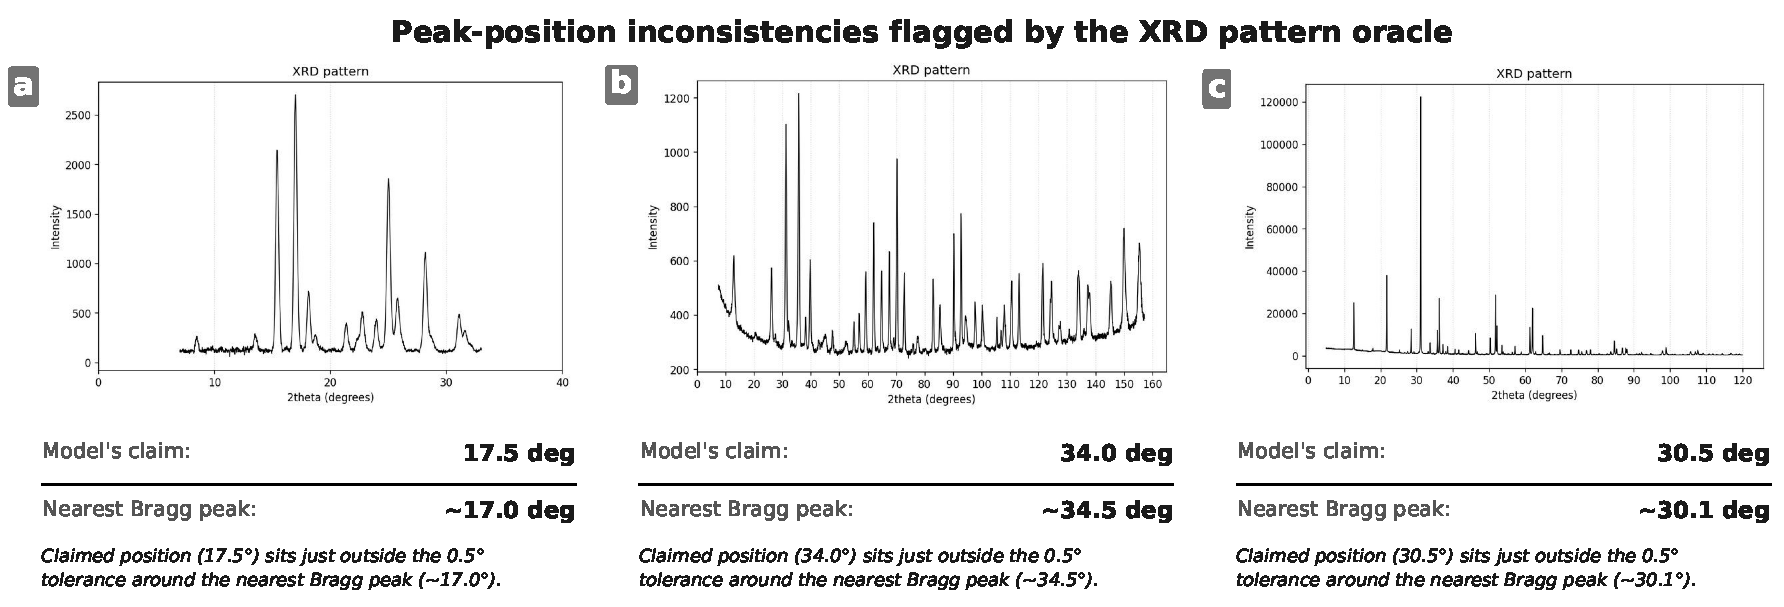
\includegraphics[width=\linewidth]{new_xrd_oracle_figure.pdf}
%\caption{\textbf{Peak-position inconsistencies flagged by the diffraction oracle.} Three
%real, human-confirmed oracle-fired cases: the model's claimed $2\theta$ position, the
%nearest genuine Bragg reflection in the same real diffractogram, and the resulting
%tolerance violation. All three claims sit just outside the oracle's $0.5^\circ$ tolerance
%window around a real peak, consistent with the tolerance-driven false-positive pattern
%described above.}
%\label{fig:xrd-oracle-examples}
%\end{figure}

%\begin{figure}[t]
%\centering
%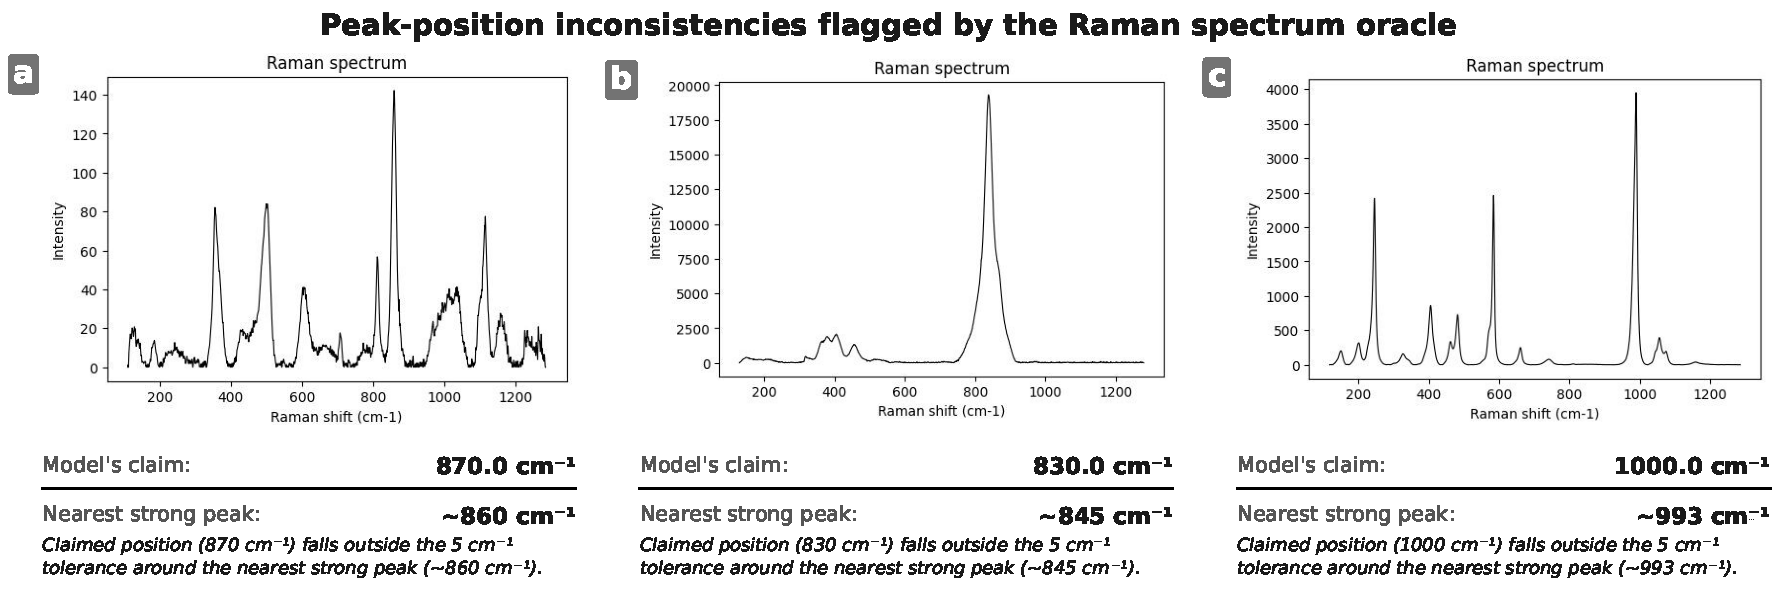
\includegraphics[width=\linewidth]{new_raman_oracle_figure.pdf}
%\caption{\textbf{Peak-position inconsistencies flagged by the Raman spectrum oracle.}
%Three real, human-confirmed oracle-fired cases: the model's claimed Raman shift, the
%nearest genuine strong peak in the same real spectrum, and the resulting tolerance
%violation. All three claims sit just outside the oracle's %$5\,\mathrm{cm}^{-1}$ tolerance
%window around a real peak, the same root cause identified for 34 of 36 %(94\%) of the
%revised spectrum oracle's false positives.}
%\label{fig:raman-oracle-examples}
%\end{figure}

%\begin{figure}[t]
%\centering
%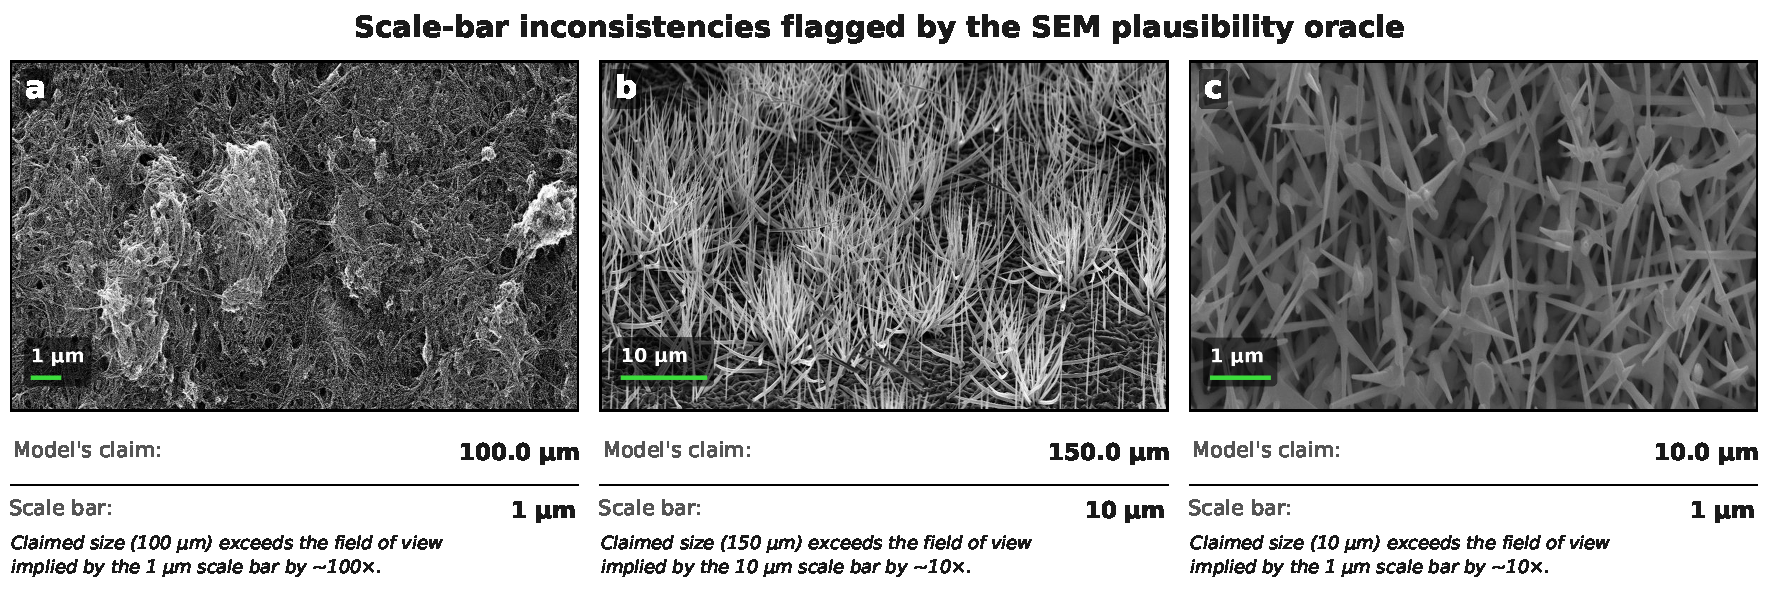
\includegraphics[width=\linewidth]{new_sem_oracle_figure.pdf}
%\caption{\textbf{Scale-bar inconsistencies flagged by the microscopy oracle.} Three real,
%human-confirmed oracle-fired cases: the model's claimed feature size against the real,
%burned-in scale bar of the same NFFA-EUROPE micrograph. Claimed sizes exceed the field of
%view the scale bar implies by roughly $10$--$100\times$, consistent with the scale-bar
%unit and scale-factor arithmetic errors that dominate the microscopy violation taxonomy
%(Results).}
%\label{fig:sem-oracle-examples}
%\end{figure}



\begin{figure}[!htbp]
    \centering

    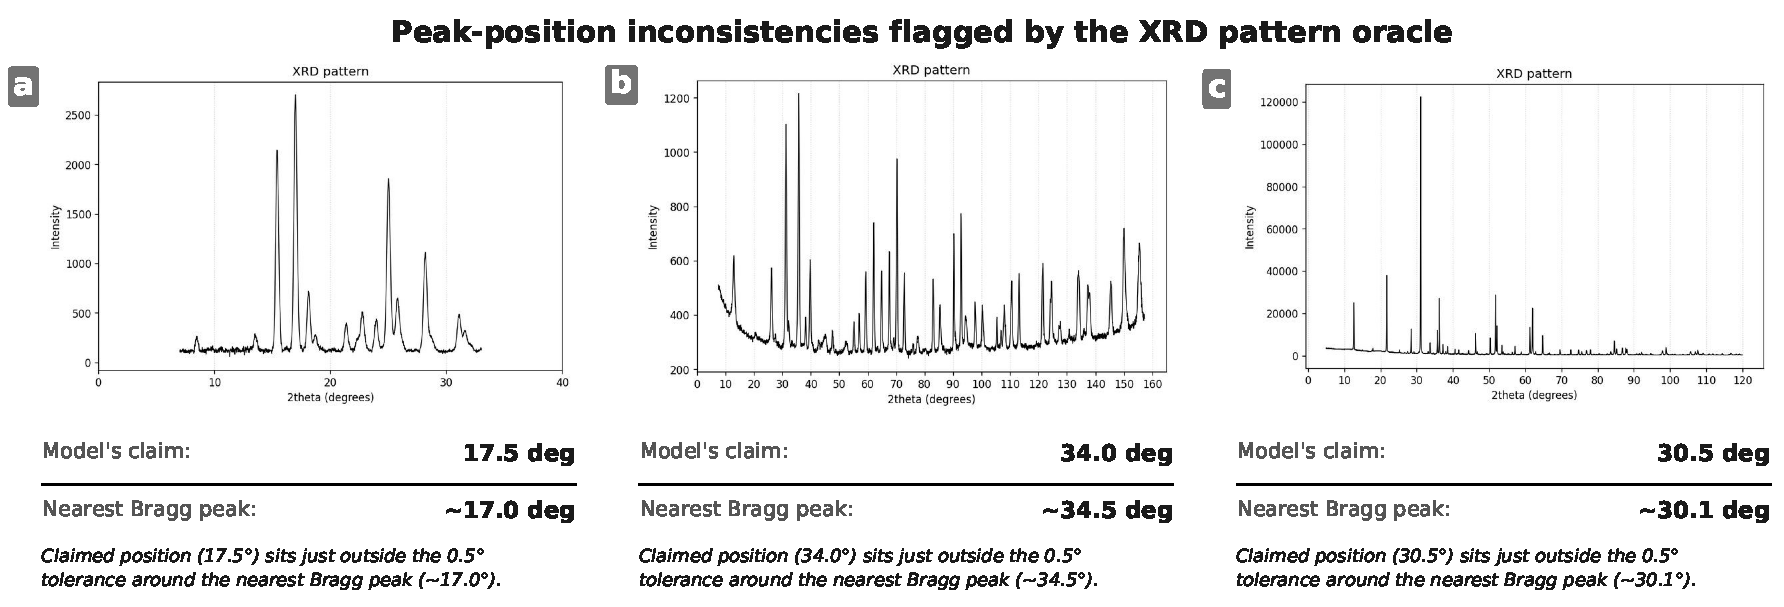
\includegraphics[width=\linewidth,height=0.235\textheight,keepaspectratio]
    {new_xrd_oracle_figure.pdf}

    \vspace{1mm}

    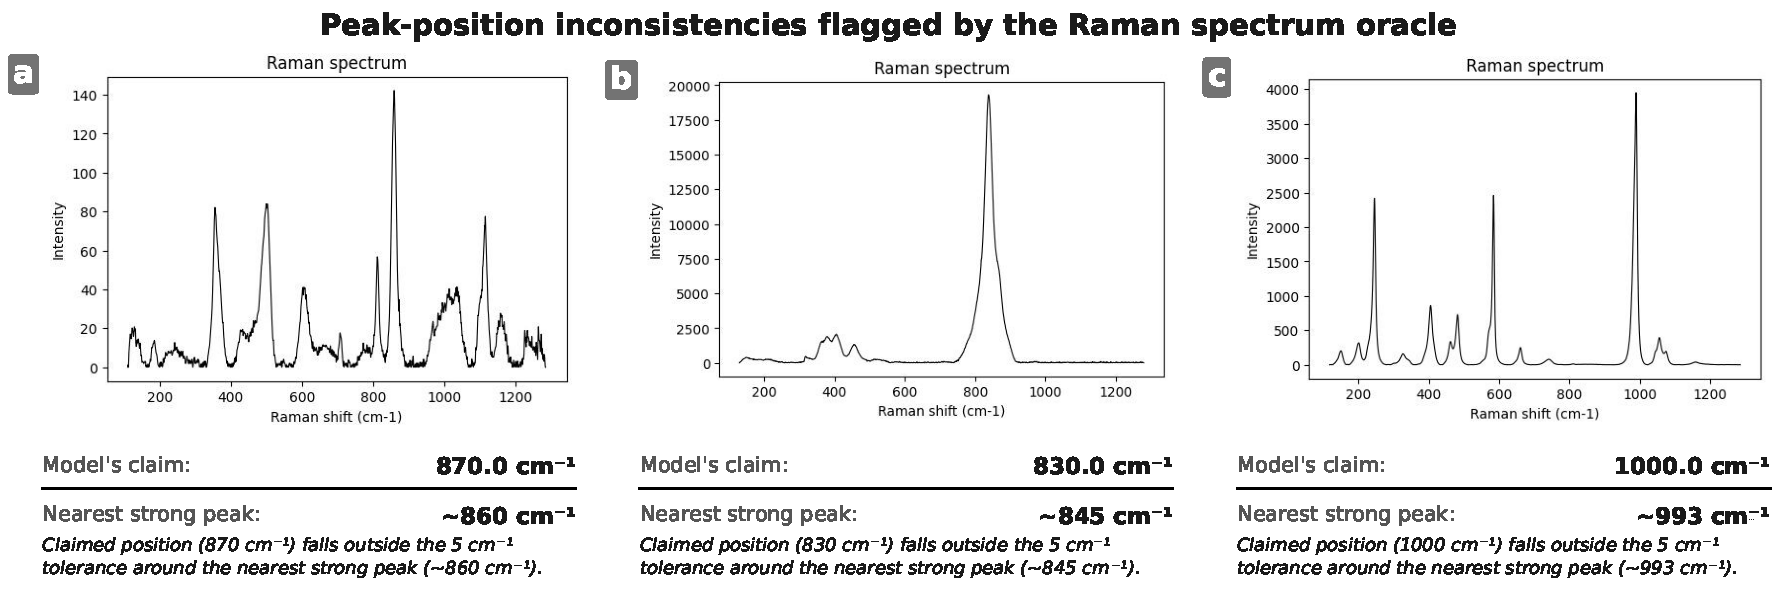
\includegraphics[width=\linewidth,height=0.235\textheight,keepaspectratio]
    {new_raman_oracle_figure.pdf}

    \vspace{1mm}

    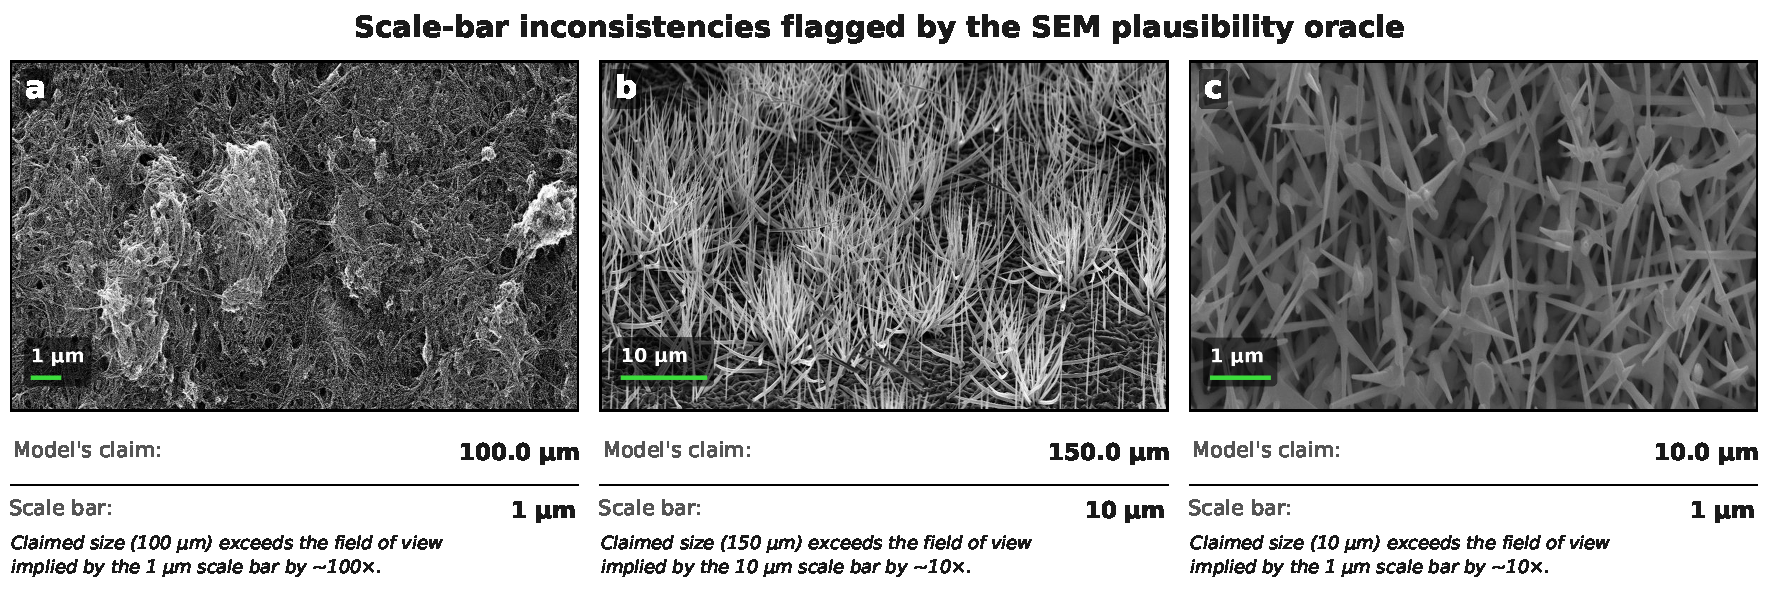
\includegraphics[width=\linewidth,height=0.235\textheight,keepaspectratio]
    {new_sem_oracle_figure.pdf}

    \caption{\justifying\textbf{Representative inconsistencies identified by the multimodal
    oracles.}
    \textbf{a}, X-ray diffraction cases in which the model-reported
    $2\theta$ position lies outside the $0.5^\circ$ tolerance around the nearest
    genuine Bragg reflection.
    \textbf{b}, Raman spectroscopy cases in which the model-reported Raman shift
    exceeds the $5\,\mathrm{cm}^{-1}$ tolerance relative to the nearest genuine
    spectral peak.
    \textbf{c}, Microscopy cases in which the model-reported feature size is
    inconsistent with the physical scale indicated by the embedded scale bar,
    producing discrepancies of approximately $10$--$100\times$.
    All examples are human-confirmed oracle activations and illustrate
    representative tolerance, unit-conversion, and scale-factor failure modes.}

    \label{fig:oracle-examples}
\end{figure}



\begin{table}[t]
\centering
\caption{\justifying\textbf{Oracle validity and audited precision.} The positive-control
false-negative rate is the maximum across three planted violation rates (10\%, 30\%, and 50\%);
all three rates yielded 0.0000 for every oracle family\rev{, which measures completeness on the
injected violation types only}. Audited precision is the fraction of oracle-fired cases from
Qwen2.5-VL-7B and Gemini 2.5 Flash Lite outputs that human review confirmed as genuine
violations of the stated constraint rather than parsing or oracle artifacts\rev{, with Wilson
95\% intervals; $n$ counts decided cases (2 spectrum cases marked unsure are excluded; counting
them either way gives 92.3--92.7\%). Every audit was sampled and judged under the final oracle
definitions used for all reported results (Methods): spectrum responses were collected once and the fired
set re-scored with the final oracle before the audit, and DFT responses were re-collected under the final
definitions before the audit; the diffraction and microscopy audits were carried out in July 2026 and the others in August 2026. Sources: NFFA, NFFA-EUROPE; MP, Materials Project.
$^{a}$Final stability oracle with the near-hull abstention band: the 50 audited cases with
$0<E_{\mathrm{hull}}\le0.05$ eV\,atom$^{-1}$ are not scored; under the original rule the audit gave 95.3\%
[89.5, 98.0] ($n=107$). Consensus: a second annotator, blind to the first labels, re-labelled a random
subsample of 30 audited cases per family stratified by the first annotator's verdict, and the two annotators
adjudicated together every case on which they disagreed (24 in total); the consensus precision is weighted back
to the audited population by stratum, with 95\% intervals from per-stratum Jeffreys posteriors (30 subsampled
cases per family; $^{b}$14, the subsampled stability cases scored under the final oracle). Agreement statistics and the oracle-silent audit are in Supplementary Table~S8.
The full audits were performed by one annotator (R.K.).}}
\label{tab:exp1}
{\scriptsize\setlength{\tabcolsep}{2.5pt}\renewcommand{\arraystretch}{1.12}
\begin{tabular}{l l S[table-format=1.4] c c}
\toprule
Oracle family & Source & {FN rate} & \multicolumn{2}{c}{Audited precision, \% [95\% CI]} \\
\cmidrule(lr){3-3}\cmidrule(lr){4-5}
& & {\itshape positive control} & {\itshape one annotator ($n$)} & \rev{\itshape two-annotator consensus} \\
\midrule
\multicolumn{5}{l}{\itshape Geometric oracles}\\
Diffraction & opXRD & 0.0000 & 77.2 \rev{[68.1, 84.3]} (101) & \rev{60.2 [44.1, 75.4]} \\
Microscopy & NFFA       & 0.0000 & 88.6 \rev{[81.1, 93.3]} (105) & \rev{88.6 [81.8, 93.9]} \\
Raman spectra & RRUFF & 0.0000 & 92.7 \rev{[90.1, 94.7]} (493) & \rev{60.8 [43.6, 76.3]} \\
\addlinespace
\multicolumn{5}{l}{\itshape DFT-grounded oracles}\\
Stability & MP & 0.0000 & \rev{100 [93.7, 100] (57)$^{a}$} & \rev{100 [84.3, 100]$^{b}$} \\
Metallicity & MP & 0.0000 & 94.7 \rev{[89.0, 97.6]} (114) & \rev{94.7 [86.8, 97.0]} \\
Magnetism & MP & 0.0000 & 92.2 \rev{[85.8, 95.8]} (115) & \rev{91.4 [79.9, 96.5]} \\
\bottomrule
\end{tabular}}
\end{table}

\subsection*{Physical consistency of current models}
We measure the Physical-Consistency Rate and per-constraint-type violation rates for
the four originally evaluated models, four later-generation frontier or open models, and
one flagship-tier addition
across diffraction, microscopy, spectra, and
DFT-grounded constraints, separately for image (VLM) and structure or text (LLM)
inputs (Table~\ref{tab:main}, Fig.~\ref{fig:results}a)\rev{. Each (model, constraint-type) cell
sends 30 items per seed to the model, with $S=3$ seeds (90 items per cell); 4{,}334 of these
responses are scored across the nine models. For the image constraint types all nine models
receive the same items in each seed, so their comparisons are paired; for the DFT constraint
types each model and seed draws its own block of materials, so those comparisons are unpaired.
Not every attempted item can be scored. On diffraction, 64 of the 90 items per cell have a
reference pattern the oracle can use (the rest lack a usable structure); on metallicity, 1--8
items per cell fall in the oracle's abstention band, and on stability 11--19 items per cell are
near-hull materials, which the final stability oracle does not score (Methods). Within the items the oracle can score, the
share of responses that state a checkable quantity (coverage) is at least 0.93 in every cell
except GPT-4o on spectra (0.49; Supplementary Table~S2).} Overall PCR ranges from \rev{0.556
(Qwen3-VL-8B-Instruct) to 0.778 (GPT-5.6-Sol, with GPT-5.6-Terra at 0.777)}; models are
markedly more consistent on microscopy (0.67--1.00) than on spectra (0.07--0.83) or
diffraction (0.47--0.82), and the DFT-grounded column is more tightly clustered
(\rev{0.65--0.76}) than any single geometric constraint\rev{.}

\rev{Because PCR excludes responses that state no checkable quantity, a model could in
principle raise its score by stating less. We therefore also scored every cell under two
alternative conventions: counting a non-checkable response as a violation (penalised) and as
consistent (lenient). The overall ordering of the nine models is nearly unchanged (Kendall
$\tau=0.83$ between the reported and penalised conventions and $1.00$ between the reported and
lenient ones); the main change is GPT-4o, from third to fifth under the penalised
convention, because of its low coverage on spectra (Supplementary Table~S2).}

\rev{We test model differences at the item level rather than by comparing interval overlap:
exact McNemar tests on the paired image-arm items, Fisher exact tests on the unpaired DFT items,
and, for overall PCR, a bootstrap that resamples paired items jointly and DFT items within
model (Methods). Holm correction is applied within each family of comparisons (Supplementary
Table~S3). GPT-5.6-Terra exceeds GPT-4o overall by 0.072 (95\% CI $[0.018,0.125]$, Holm
$p=0.045$). Claude Opus 4.6 versus Claude Sonnet 4.5 ($-0.003$, $[-0.050,0.044]$),
Qwen3-VL-8B-Thinking versus Qwen3-VL-8B-Instruct ($+0.034$, $[-0.016,0.083]$) and
GPT-5.6-Sol versus GPT-5.6-Terra ($+0.002$, $[-0.042,0.046]$) are not significant. With
roughly 500 checkable items per model, the smallest overall difference the design detects with
80\% power is 0.064--0.079 depending on the pair, so these three comparisons exclude only
differences larger than about 0.07; they do not show that the models are equivalent. Across all
36 model pairs, 18 differences in overall PCR survive Holm correction; within single
constraint types the detectable difference is 0.11--0.20, so most per-type rankings are not
resolved. On microscopy, the locally run Qwen2.5-VL-7B is the weakest model (0.667, 95\% CI
$[0.563,0.759]$), and seven of the other eight models exceed it after Holm correction (paired
differences $+0.22$ to $+0.33$), while Qwen3-VL-8B-Instruct ($+0.14$, Holm $p=0.12$) does not.} We do not
know whether the gap reflects genuine scale-bar-reading skill or a difference in how each model handles the
info-bar layout variety in the source micrographs, and do not claim more than the
measured difference. The high absolute microscopy rates should also be read against the
looseness of this oracle, which flags only feature sizes exceeding the field of view (a
necessary, not sufficient, condition), so a near-ceiling rate partly reflects an easily
satisfied check. \rev{Diffraction comparisons in particular should be treated as provisional:
the diffraction ranking changes both when the oracle tolerance is varied and when the prompt is
paraphrased (Methods).}

\rev{The DFT column is also sensitive to class composition. The sampled materials are
imbalanced (for stability, only 3--9 of the 70--79 scored materials per model lie on the hull), so a
model that defaults to the majority answer scores well on pooled PCR. Qwen2.5-VL-7B reaches a pooled
stability PCR of 0.917 but answers none of its 4 on-hull materials consistently, a class-balanced rate
of 0.485, whereas GPT-5.6-Terra has the lowest pooled stability PCR (0.653) but a class-balanced rate of
0.814 (Supplementary Table~S4); with so few on-hull materials per model, these class-balanced rates are
imprecise. The ordering of models on the DFT constraint types therefore depends on whether PCR is pooled
or class-balanced, and we report both. To make the DFT comparisons paired as well, we evaluated the
models on one common item set of 90 materials per DFT constraint type, drawn 45 from each reference
class (Supplementary Table~S6); for stability, 34 of the 45 near-hull draws fall in the band the final
oracle does not score, leaving 56 scored materials (11 on the hull, 45 above it). Eight models are
included; Qwen3-VL-8B-Thinking could not be run because its provider endpoint had been withdrawn by the
time of this analysis, and the locally run Qwen2.5-VL-7B was run on CPU in single precision, because no
GPU with bfloat16 support was available then. On this paired set, restricted to the DFT constraint
types, none of the comparisons stated above is significant: GPT-5.6-Terra versus GPT-4o $+0.021$ (95\% CI
$[-0.042,0.085]$), Claude Opus 4.6 versus Claude Sonnet 4.5 $+0.021$ ($[-0.030,0.072]$) and GPT-5.6-Sol
versus GPT-5.6-Terra $+0.030$ ($[-0.013,0.072]$); 3 of the 28 model pairs differ after Holm correction,
all of them Gemini 2.5 Flash Lite scoring lower. The difference between GPT-5.6-Terra and GPT-4o in the
main evaluation therefore comes from the image constraint types, chiefly spectra. The balanced set also
shows a shared failure that the imbalanced sample hid: every model is far less consistent on
computed-metallic compositions (PCR 0.21--0.40) than on gapped ones (0.84--0.96), that is, models
default to calling a composition non-metallic.}

\begin{table}[t]
\centering
\caption{\justifying Main evaluation: Physical-Consistency Rate by constraint type and overall,
\rev{over the checkable responses among 30 attempted items} per (model, constraint-type) cell per seed, $S=3$ seeds pooled per cell
(bootstrap 95\% CIs omitted from this compact view; see Supplementary Table~S1 for the
full per-cell confidence intervals \rev{and checkable counts, Supplementary Table~S2 for coverage
and alternative conventions, Supplementary Table~S3 for paired, Holm-corrected model comparisons,
and Supplementary Table~S4 for class-balanced DFT rates}, and the Methods for why $\rho_t=1-\mathrm{PCR}$ here). DFT column combines the stability, metallicity,
and magnitude constraint types\rev{; near-hull stability materials are not scored (Methods; the original
rule's values are in Supplementary Table~S7)}.  The first four rows are the
originally evaluated models; the next four are the later-generation refresh
(Methods, Baselines subsection). $^{\ddagger}$GPT-5.6-Sol is OpenAI's flagship tier, added
to test whether it exceeds the balanced-tier GPT-5.6-Terra within the same
generation; \rev{the overall difference is $+0.002$ (95\% CI $[-0.042,0.046]$), not significant, so
the design detects no difference between flagship and balanced tier larger than about 0.07}
(Discussion). \rev{Bold marks the column maximum; it does not imply a significant difference from
the next model.}}
\label{tab:main}
{\scriptsize\setlength{\tabcolsep}{5pt}\renewcommand{\arraystretch}{1.12}
\begin{tabular}{l *{5}{S[table-format=1.3]}}
\toprule
& \multicolumn{5}{c}{Physical-Consistency Rate (higher is more consistent)} \\
\cmidrule(lr){2-6}
Model & {Diffraction} & {Microscopy} & {Spectra} & {DFT$^{*}$} & {All$^{*}$} \\
\midrule
Qwen2.5-VL-7B \textit{(open)} & 0.500 & 0.667 & 0.148 & \rev{0.731} & \rev{0.584} \\
Gemini 2.5 Flash Lite & 0.517 & \bfseries 1.000 & 0.278 & \rev{0.658} & \rev{0.630} \\
GPT-4o                & 0.625 & 0.954 & 0.068 & \rev{0.740} & \rev{0.699} \\
Claude Sonnet 4.5     & 0.547 & 0.977 & 0.189 & \bfseries \rev{0.762} & \rev{0.667} \\
\addlinespace
Claude Opus 4.6            & 0.578 & 0.954 & 0.244 & \rev{0.734} & \rev{0.663} \\
GPT-5.6-Terra              & 0.797 & 0.951 & \bfseries 0.833 & \rev{0.696} & \rev{0.777} \\
Qwen3-VL-8B-Instruct       & 0.468 & 0.802 & 0.133 & \rev{0.649} & \rev{0.556} \\
Qwen3-VL-8B-Thinking       & 0.578 & 0.885 & 0.092 & \rev{0.671} & \rev{0.594} \\
\addlinespace
GPT-5.6-Sol$^{\ddagger}$   & \bfseries 0.820 & 0.915 & 0.764 & \rev{0.727} & \bfseries \rev{0.778} \\
\bottomrule
\end{tabular}}
\end{table}


\subsection*{Accuracy versus consistency}
On three constraint types with a genuine, non-circular accuracy criterion distinct
from the oracle's own tolerance (diffraction: agreement with the single nearest true
peak to $0.1^{\circ}$, versus the oracle's looser $0.5^{\circ}$ tolerance; spectra:
agreement with the nearest real measured peak to $2\,\mathrm{cm}^{-1}$, versus the
oracle's prominence-based check; stability: agreement with the Materials
Project \texttt{is\_stable} label, evaluated separately from the oracle's
operational $0.05\,\mathrm{eV\,atom^{-1}}$ near-hull threshold), we report
accuracy alongside PCR and the four-cell breakdown on the same
\rev{838 scored items} ($n=30$ per (model, constraint-type) cell, $S=3$ seeds\rev{, the four originally evaluated
models; this sample is drawn separately from the main evaluation}). Microscopy is excluded: its
prompt elicits only a feature-size claim, so no non-circular accuracy ground truth is
available without a different prompt design. \rev{On the eight diffraction and spectra cells,
accuracy and PCR disagree on a mean of 23.6\% of items, and on stability they coincide
(Fig.~\ref{fig:pipeline}b,c). Part of the diffraction and spectra disagreement is definitional rather
than evidence of reasoning errors that accuracy misses: the accuracy criteria are deliberately tighter
than the oracle tolerances, so the two scores are expected to differ on items that fall between the two
thresholds. What the comparison does establish is that
the two scores measure different properties of the same response, not that PCR detects errors that
accuracy cannot.} Diffraction is dominated by items
that are wrong by the tight accuracy criterion yet still oracle-consistent (up to 36
of 62 items in one diffraction cell, gap 58.1\%): models are frequently close enough to satisfy the
oracle's looser tolerance while measurably off the exact peak. \rev{On spectra, most responses
are wrong by both criteria, so the two scores disagree on few items} (4.2--11.2\% across models). \rev{On stability the two scores coincide under the final protocol,
and this is informative in itself. The oracle's $0.05\,\mathrm{eV\,atom^{-1}}$ near-hull threshold and
Materials Project's own \texttt{is\_stable} label (true only on the hull) disagree on 571 of 3,000 real
entries (19.0\%), and every one of those is a near-hull material, $0<E_{\mathrm{hull}}\le0.05$. The final
oracle does not score that band (Methods), so outside it the two definitions agree, and the stability gap
of 18.0--27.8\% reported under the original rule came entirely from the near-hull materials. The stability
arm still shows the base-rate confound: Qwen2.5-VL-7B is accurate on 61 of 62 unstable materials but on
none of the 8 stable ones, so its near-ceiling raw accuracy reflects the base rate rather than
discriminative skill. Balanced accuracy (the mean of per-class accuracy) is 0.492 (Qwen2.5-VL-7B), 0.690
(Gemini 2.5 Flash Lite), 0.492 (GPT-4o) and 0.992 (Claude Sonnet 4.5); two of the four models are at
chance once the imbalance is corrected for ($n=65$--73 scored materials per model, 5--8 of them stable).}

\rev{What PCR adds to answer accuracy is therefore not a finer measure of correctness but a
different, label-free property. First, it needs no answer key: it is defined on microscopy and
on net magnetization, where this benchmark has no non-circular accuracy criterion, and on any new
item for which a reference structure, scale bar or computed value exists. Second, it is a floor
rather than a target: a violation is a statement the measurement or the reference calculation
rules out, so a violation is informative about the reasoning that produced it (Fig.~\ref{fig:teaser}c
shows what these violations consist of), whereas an accuracy miss may only reflect reading
precision. Third, because it is a necessary condition, PCR cannot certify that a response is
right; a high PCR with low accuracy, as on diffraction, identifies responses that are physically
admissible but imprecise. We therefore present PCR as a complement to answer accuracy where labels
exist and as a substitute screening signal where they do not, not as a replacement for either.}

\subsection*{Effect of self-verification}
We measure PCR before and after CGSV on identical items and test the change with the
exact paired McNemar test, reporting fixes, regressions, and residual violations
(Table~\ref{tab:cgsv}, Fig.~\ref{fig:results}b), on diffraction and spectra, the two constraint types where
the oracle's feedback is an actionable physical constraint the model can re-examine
without the feedback message itself revealing the answer (a scale-bar violation
message would state the conversion factor outright, and the three DFT claim types are
single-shot binary judgments with no intermediate quantity to reconsider). $n=30$
items per (model, constraint-type) cell, $S=3$ seeds, $K=2$ maximum revision rounds, 545
checkable records in total. \rev{Because Algorithm~\ref{alg:cgsv} stops at the first round in which no
violation remains, an item that is consistent before revision is never revised. The absence of
regressions in consistency ($b=0$ in every cell) therefore follows from the stopping rule; it
confirms the implementation but is not evidence about the model.} CGSV raises PCR for all four models pooled across both
constraint types (Qwen2.5-VL-7B $0.338\!\to\!0.439$, $p=3.1\times10^{-5}$; Gemini 2.5
Flash Lite $0.521\!\to\!0.632$, $p=2.4\times10^{-4}$; GPT-4o
$0.434\!\to\!0.593$, $p=7.6\times10^{-6}$; Claude Sonnet 4.5 $0.373\!\to\!0.639$,
$p=4.6\times10^{-13}$\rev{; all survive Holm correction}).
Residual violations remain in every cell after $K=2$ rounds (roughly 40--90\% of
items \rev{on spectra}), so CGSV reduces but does not eliminate violations.

\rev{Because CGSV is scored by the same oracles that supply its feedback, a rise in PCR alone cannot
show that revised answers are more correct. Every item exposes exactly one checkable claim in
every round, so a gain cannot come from the model dropping the claim. To see what the revisions
achieve, we scored each item's first-round and final-round claim against the same non-circular
accuracy criteria as the accuracy-versus-consistency analysis ($0.1^\circ$ for diffraction,
$2\,\mathrm{cm}^{-1}$ for spectra) and compared them on the same items (Table~\ref{tab:cgsvacc}).
Accuracy is a property the loop never observes, so unlike consistency it can regress. On spectra
($n=293$) accuracy rises from 5.8\% to 9.9\%: 14 items become accurate and 2 cease to be (exact
McNemar $p=0.004$). Of the 244 spectrum items the oracle flagged and the model revised, 48 cleared
the oracle; 11 of these moved to the accurate value and 37 to a value the oracle admits but that
is not within the accuracy tolerance, and the remaining 196 stayed inconsistent.
On diffraction ($n=245$; 7 items whose reference pattern could not be computed are omitted) accuracy
rises from 22.9\% to 28.6\%: 14 items become accurate and none ceases to be (exact McNemar $p=0.0001$).
Of the 79 diffraction items the oracle flagged and the model revised, 41 cleared the oracle; 14 of these
moved to the accurate value and 27 to an admissible but inexact one, and 38 stayed inconsistent. Revisions that clear
the oracle therefore mostly move a claim into the physically admissible region rather than onto the
exact value, while also producing a small but significant net gain in correctness. The evidence
supports this narrower statement, not a claim that CGSV corrects the underlying physics in general.}

\rev{We separately ask whether the gain is}
attributable to the oracle signal specifically, or to extra inference-time compute alone,
with three controls matched to CGSV's items, models, and decoding
(Baselines subsection): unaided self-refinement (the model is told to double-check its
answer with no oracle feedback) shows no significant change (before $0.349$, after $0.339$, $n=542$, $b=34$, $c=29$, $p=0.615$);
generic equal-compute re-prompting (the model is simply asked to reconsider) likewise shows
no significant change (before $0.358$, after $0.342$, $n=562$, $b=24$, $c=15$, $p=0.20$). \rev{Both
controls revise every item, including those already consistent, so their nonzero regression counts
are not comparable with CGSV's structural $b=0$; the comparison that matters is the net change,
which is significant for CGSV and absent for both controls.} Best-of-3 independent resampling gives a
random-pick PCR of $0.363$ and an oracle-oracle upper bound (best of 3) of $0.419$
($n=614$). Both fall below CGSV's oracle-guided after-PCR for every model, though the
margin over the weakest, Qwen2.5-VL-7B at $0.439$, is only $0.02$, and the resampling run
draws its own item sample, so we do not test the difference. \rev{These controls show that the PCR gain
is not reproduced by generic self-reflection or by extra sampling at equal compute; they do not
by themselves show that the gain reflects better physics, which is what the paired correctness
analysis above addresses.}

\begin{table}[t]
\centering
\caption{\justifying Effect of Constraint-Grounded Self-Verification, pooled across diffraction
and spectra, $n=30$ items per (model, constraint-type) cell, $S=3$ seeds, $K=2$ rounds.
$\Delta$: PCR gain (after minus before); $b$: regressions (before-consistent,
after-inconsistent); $c$: fixes (before-inconsistent, after-consistent); $p$: exact
two-sided McNemar test on $(b,c)$; $p_{\mathrm{Holm}}$: Holm-Bonferroni-adjusted $p$ over
this table's 6-test family (Methods, Statistics paragraph). All four CGSV effects survive
this correction; both controls remain non-significant. \rev{For CGSV, $b=0$ follows from the stopping
rule (an item consistent before revision is never revised); the controls revise every item, so
their $b$ is not comparable. Paired changes in correctness are in Table~\ref{tab:cgsvacc}.}}
\label{tab:cgsv}
{\scriptsize\setlength{\tabcolsep}{3.4pt}\renewcommand{\arraystretch}{1.12}
\begin{tabular}{l S[table-format=1.3] S[table-format=1.3] S[table-format=+1.3] S[table-format=2.0] S[table-format=2.0] c c}
\toprule
& \multicolumn{3}{c}{PCR} & \multicolumn{2}{c}{Discordant} & & \\
\cmidrule(lr){2-4}\cmidrule(lr){5-6}
Model & {before} & {after} & {$\Delta$} & {$b$} & {$c$} & {$p$} & {$p_{\mathrm{Holm}}$} \\
\midrule
Qwen2.5-VL-7B         & 0.338 & 0.439 & 0.101 & 0 & 16 & $3.1\times10^{-5}$ & $1.2\times10^{-4}$ \\
Gemini 2.5 Flash Lite & 0.521 & 0.632 & 0.111 & 0 & 13 & $2.4\times10^{-4}$ & $7.3\times10^{-4}$ \\
GPT-4o                & 0.434 & 0.593 & \bfseries 0.159 & 0 & 18 & $7.6\times10^{-6}$ & $3.8\times10^{-5}$ \\
Claude Sonnet 4.5     & 0.373 & 0.639 & \bfseries 0.266 & 0 & 42 & $4.6\times10^{-13}$ & $2.7\times10^{-12}$ \\
\midrule
\multicolumn{8}{l}{\itshape Mechanism-isolation controls (pooled across models, both constraint types)}\\
Self-refinement (no oracle) & 0.349 & 0.339 & -0.010 & 34 & 29 & 0.615 & 0.615 \\
Generic re-prompting        & 0.358 & 0.342 & -0.016 & 24 & 15 & 0.20 & 0.399 \\
\bottomrule
\end{tabular}}
\end{table}

\begin{table}[t]
\revon\centering
\caption{\justifying Paired change in answer correctness before and after CGSV, on the same items as
Table~\ref{tab:cgsv}. Accuracy uses the non-circular criteria of the accuracy-versus-consistency
analysis (diffraction: within $0.1^\circ$ of the nearest reference reflection; spectra: within
$2\,\mathrm{cm}^{-1}$ of the nearest detected local maximum), applied to each item's first-round
and final-round claim (accuracy before$\to$after). L/G: items that stop (lost) or start (gained) being
accurate; $p$: exact two-sided McNemar test on (L, G). Rev.: items the oracle flagged at round 1 and the
model revised; of these, A cleared the oracle with an accurate value, Ad cleared it with an admissible
value outside the accuracy tolerance, and U were still flagged after $K=2$ rounds.}
\label{tab:cgsvacc}
{\scriptsize\setlength{\tabcolsep}{2.5pt}\renewcommand{\arraystretch}{1.12}
\begin{tabular}{l l r c c r r c}
\toprule
Constraint & Model & $n$ & Accuracy & L/G & $p$ & Rev. & A/Ad/U \\
\midrule
Spectra & Qwen2.5-VL-7B & 89 & 0.067$\to$0.101 & 0/3 & 0.25 & 80 & 3/9/68 \\
 & Gemini 2.5 F.\ Lite & 69 & 0.043$\to$0.072 & 0/2 & 0.50 & 49 & 2/6/41 \\
 & GPT-4o & 45 & 0.044$\to$0.044 & 1/1 & 1.00 & 40 & 0/4/36 \\
 & Claude Sonnet 4.5 & 90 & 0.067$\to$0.144 & 1/8 & 0.039 & 75 & 6/18/51 \\
 & \textit{pooled} & 293 & 0.058$\to$0.099 & 2/14 & 0.004 & 244 & 11/37/196 \\
\addlinespace
Diffraction & Qwen2.5-VL-7B & 66 & 0.303$\to$0.318 & 0/1 & 1.00 & 24 & 1/3/20 \\
 & Gemini 2.5 F.\ Lite & 47 & 0.213$\to$0.255 & 0/2 & 0.50 & 7 & 2/3/2 \\
 & GPT-4o & 66 & 0.152$\to$0.212 & 0/4 & 0.12 & 24 & 4/10/10 \\
 & Claude Sonnet 4.5 & 66 & 0.242$\to$0.348 & 0/7 & 0.016 & 24 & 7/11/6 \\
 & \textit{pooled} & 245 & 0.229$\to$0.286 & 0/14 & 0.0001 & 79 & 14/27/38 \\
\bottomrule
\end{tabular}}
\end{table}

\subsection*{Verifier for violation prediction}
We fine-tune Qwen2.5-0.5B-Instruct with LoRA on oracle-derived labels alone (no human
annotation) to predict, from the input description and chain text alone, whether a
physical violation is present, using 2{,}152 real oracle-checked records spanning all
six constraint types collected across the preceding evaluations. We report precision,
recall, $F_1$, ROC AUC, and expected calibration error (ECE) on an 80/20
in-distribution split and separately on six held-out-constraint-type splits (train on the
other five constraint types, test on one entirely unseen one). The in-distribution split
is disjoint at the parent source (item or structure) level, \rev{so no source item contributes
records to both sides}. In distribution the verifier is a useful
detector overall (precision 0.77, recall 0.71, $F_1=0.74$, AUC $=0.850$, ECE $=0.096$).
\rev{This pooled figure overstates its usefulness for a given scientific task, for two reasons.
First, the six families have very different violation base rates (19\% for microscopy to 88\%
for spectra in the test split), so a score that only identified the family would already rank
violations above chance: a baseline that assigns each item its family's training-set violation
rate reaches AUC $=0.759$. Second, within single families the verifier's discrimination varies
widely (Table~\ref{tab:verifierfam}): it is strong on microscopy (AUC $0.922$, 95\% CI
$[0.852,0.977]$) and stability ($0.804$, $[0.683,0.903]$), moderate on magnetism ($0.728$,
$[0.562,0.877]$) and diffraction ($0.696$, $[0.493,0.895]$), and not distinguishable from chance on
metallicity ($0.582$, $[0.390,0.775]$) and spectra ($0.513$, $[0.353,0.702]$). The in-distribution
verifier is therefore a useful triage signal for microscopy and stability claims, a weak one for
magnetism and diffraction, and not useful for metallicity or spectra.} Its
cross-constraint-type generalization is poor for all six constraint types: diffraction, microscopy, and stability
are indistinguishable from chance when held out entirely (AUC 0.50, 0.53, and 0.44,
bootstrap 95\% confidence intervals straddling 0.5), spectra is not separable from chance either (AUC
0.56, CI $[0.488,0.626]$)\rev{, magnetism is at chance (AUC $0.503$, $[0.430,0.576]$),} and metallicity is the single arguable exception, with a nominal
95\% interval that excludes chance (AUC 0.58, CI $[0.510,0.652]$) but that no longer does so
once the interval is widened for the six held-out comparisons (Bonferroni-corrected interval
$[0.487,0.673]$). We therefore treat metallicity as a nominal, uncorrected exception rather
than as evidence of transfer, and do not build any claim on it. \rev{No held-out constraint type shows transfer that survives correction for the six comparisons.} We report the verifier as an
in-distribution tool \rev{for the families where it discriminates}, and explicitly do \emph{not} claim it as a general-purpose,
constraint-agnostic violation detector. A pooled AUC across all six held-out constraint
types is not reported: the six held-out runs are separately fine-tuned models, so their raw
probability outputs are not on a directly comparable scale; we report only the six
per-constraint-type numbers (Table~\ref{tab:verifier}, Fig.~\ref{fig:results}c). \rev{The held-out results are sensitive to the training run. The released adapters, retrained
with the same data, splits and seed but in a different numerical precision (Supplementary Note~2),
reproduce the in-distribution AUC exactly ($0.850$) but move the held-out AUCs by up to $0.08$: held-out
microscopy rises to $0.602$, whose interval excludes chance even after Bonferroni correction
($[0.519,0.682]$), and held-out stability falls to $0.383$, below chance. No held-out family reaches a
level useful for triage in either run, which is the conclusion we draw. The verifier was trained on
oracle labels produced under the original stability rule; evaluated only on the test items that the final
oracle scores, its in-distribution AUC is $0.871$ ($[0.834,0.904]$; stability family $0.911$) and its
held-out stability AUC $0.372$, so the conclusions above do not depend on the near-hull band
(Supplementary Note~2).}

\begin{table}[t]
\centering
\caption{\justifying Verifier precision/recall/$F_1$ (in-distribution and held-out-constraint-type
splits, both source-disjoint) and the detector's bootstrap 95\% CI on ROC AUC, predicting a
real oracle violation from held-out verifier scores. Expected calibration error is
reported in the text for the in-distribution split (ECE $=0.096$). No pooled
across-constraint-type AUC is reported (see text).}
\label{tab:verifier}
{\scriptsize\setlength{\tabcolsep}{5pt}\renewcommand{\arraystretch}{1.12}
\begin{tabular}{l S[table-format=1.3] S[table-format=1.3] S[table-format=1.3] S[table-format=1.3] c}
\toprule
& \multicolumn{3}{c}{Violation prediction} & \multicolumn{2}{c}{Detector (ROC)} \\
\cmidrule(lr){2-4}\cmidrule(lr){5-6}
Split & {Precision} & {Recall} & {$F_1$} & {AUC} & {95\% CI} \\
\midrule
\multicolumn{6}{l}{\itshape In distribution (80/20 split, source-disjoint)}\\
All constraint types & 0.768 & 0.706 & 0.735 & \bfseries 0.850 & {[}0.813, 0.883{]} \\
\addlinespace
\multicolumn{6}{l}{\itshape Held out entirely (train on the other five constraint types)}\\
Diffraction (XRD)      & 0.600 & 0.030 & 0.057 & 0.497 & {[}0.419, 0.578{]} \\
Microscopy (SEM)       & 0.239 & 0.905 & 0.378 & 0.527 & {[}0.468, 0.589{]} \\
Spectra (Raman)        & {--} & 0.000 & {--} & 0.558 & {[}0.488, 0.626{]} \\
Stability$^{*}$        & 0.355 & 0.103 & 0.159 & 0.436 & {[}0.370, 0.502{]} \\
Metallicity$^{*}$      & 0.486 & 0.158 & 0.238 & 0.582 & {[}0.510, 0.652{]} \\
Magnetism$^{*}$        & 0.468 & 0.635 & 0.539 & 0.503 & {[}0.430, 0.576{]} \\
\bottomrule
\end{tabular}}
\end{table}

\begin{table}[t]
\revon\centering
\caption{\justifying In-distribution verifier performance within each constraint family (the
source-disjoint 80/20 test split of Table~\ref{tab:verifier}, broken down by family; scores are those of
the single in-distribution model). AUC 95\% CI: bootstrap over source items ($B=5000$).
Viol.: share of test records that are oracle violations. A baseline that scores each record by
its family's training-set violation rate reaches a pooled AUC of 0.759, against the verifier's
0.850. Labels follow the original stability rule; on the items the final rule scores, the stability AUC is
0.911 (Supplementary Note~2).}
\label{tab:verifierfam}
{\scriptsize\setlength{\tabcolsep}{5pt}\renewcommand{\arraystretch}{1.12}
\begin{tabular}{l r r S[table-format=1.3] S[table-format=1.3] S[table-format=1.3] S[table-format=1.3] c}
\toprule
Family & $n$ & {Viol.} & {Precision} & {Recall} & {$F_1$} & {AUC} & {95\% CI} \\
\midrule
Diffraction (XRD)  & 33  & 70\% & 0.846 & 0.478 & 0.611 & 0.696 & {[}0.493, 0.895{]} \\
Microscopy (SEM)   & 109 & 19\% & 0.750 & 0.714 & 0.732 & 0.922 & {[}0.852, 0.977{]} \\
Spectra (Raman)    & 100 & 88\% & 0.880 & 1.000 & 0.936 & 0.513 & {[}0.353, 0.702{]} \\
Stability$^{*}$    & 87  & 31\% & 0.727 & 0.296 & 0.421 & 0.804 & {[}0.683, 0.903{]} \\
Metallicity$^{*}$  & 55  & 35\% & 0.364 & 0.421 & 0.390 & 0.582 & {[}0.390, 0.775{]} \\
Magnetism$^{*}$    & 47  & 40\% & 0.600 & 0.474 & 0.529 & 0.728 & {[}0.562, 0.877{]} \\
\bottomrule
\end{tabular}}
\end{table}

% Figure: main results (heatmap + slopegraph + forest)
\begin{figure}[p]
\centering
\resizebox{0.975\linewidth}{!}{%
\begin{tikzpicture}[font=\sffamily]
\node[plab,anchor=west] at (-0.10,7.62){a)};
\node[font=\sffamily\small\bfseries,anchor=west] at (0.55,7.62){Physical consistency by model and constraint type};
\draw[black!45,line width=0.5pt](2.57,7.10)--(6.89,7.10);
\draw[black!45,line width=0.5pt](6.92,7.10)--(11.24,7.10);
\node[font=\sffamily\fontsize{6.5}{8}\selectfont,black!60,anchor=south] at (4.73,7.14){geometric oracles};
\node[font=\sffamily\fontsize{6.5}{8}\selectfont,black!60,anchor=south] at (9.08,7.14){DFT-grounded oracles};
\node[font=\sffamily\fontsize{6.8}{8}\selectfont,anchor=south] at (3.28,6.60){Diffraction};
\node[font=\sffamily\fontsize{6}{7}\selectfont,black!55,anchor=south] at (3.28,6.30){(XRD)};
\node[font=\sffamily\fontsize{6.8}{8}\selectfont,anchor=south] at (4.73,6.60){Microscopy};
\node[font=\sffamily\fontsize{6}{7}\selectfont,black!55,anchor=south] at (4.73,6.30){(SEM)};
\node[font=\sffamily\fontsize{6.8}{8}\selectfont,anchor=south] at (6.18,6.60){Spectra};
\node[font=\sffamily\fontsize{6}{7}\selectfont,black!55,anchor=south] at (6.18,6.30){(Raman)};
\node[font=\sffamily\fontsize{6.8}{8}\selectfont,anchor=south] at (7.63,6.60){Stability};
\node[font=\sffamily\fontsize{6}{7}\selectfont,black!55,anchor=south] at (7.63,6.30){$^{*}$};
\node[font=\sffamily\fontsize{6.8}{8}\selectfont,anchor=south] at (9.08,6.60){Metallicity};
\node[font=\sffamily\fontsize{6}{7}\selectfont,black!55,anchor=south] at (9.08,6.30){$^{*}$};
\node[font=\sffamily\fontsize{6.8}{8}\selectfont,anchor=south] at (10.53,6.60){Magnetism};
\node[font=\sffamily\fontsize{6}{7}\selectfont,black!55,anchor=south] at (10.53,6.30){$^{*}$};
\node[font=\sffamily\fontsize{6.8}{8}\selectfont\bfseries,anchor=south] at (12.36,6.60){Overall};
\node[font=\sffamily\fontsize{6}{7}\selectfont,black!55,anchor=south] at (12.36,6.30){(all six)};
\node[font=\sffamily\fontsize{6.8}{8}\selectfont,anchor=east] at (2.45,5.23){GPT-5.6-Terra$^{\dagger}$};
\node[minimum width=1.42cm,minimum height=0.56cm,fill=npblue!71,draw=white,line width=1pt,inner sep=0,font=\sffamily\fontsize{7.2}{8}\selectfont,text=white] at (3.28,5.23){0.797};
\node[minimum width=1.42cm,minimum height=0.56cm,fill=npblue!84,draw=white,line width=1pt,inner sep=0,font=\sffamily\fontsize{7.2}{8}\selectfont,text=white] at (4.73,5.23){0.951};
\node[minimum width=1.42cm,minimum height=0.56cm,fill=npblue!74,draw=white,line width=1pt,inner sep=0,font=\sffamily\fontsize{7.2}{8}\selectfont,text=white] at (6.18,5.23){0.833};
\node[minimum width=1.42cm,minimum height=0.56cm,fill=npblue!60,draw=white,line width=1pt,inner sep=0,font=\sffamily\fontsize{7.2}{8}\selectfont,text=white] at (7.63,5.23){0.653};
\node[minimum width=1.42cm,minimum height=0.56cm,fill=npblue!60,draw=white,line width=1pt,inner sep=0,font=\sffamily\fontsize{7.2}{8}\selectfont,text=white] at (9.08,5.23){0.659};
\node[minimum width=1.42cm,minimum height=0.56cm,fill=npblue!69,draw=white,line width=1pt,inner sep=0,font=\sffamily\fontsize{7.2}{8}\selectfont,text=white] at (10.53,5.23){0.767};
\node[minimum width=1.42cm,minimum height=0.56cm,fill=npblue!70,draw=black!45,line width=0.6pt,inner sep=0,font=\sffamily\fontsize{7.2}{8}\selectfont\bfseries,text=white] at (12.36,5.23){0.777};
\node[font=\sffamily\fontsize{6.8}{8}\selectfont,anchor=east] at (2.45,5.85){GPT-5.6-Sol$^{\ddagger}$};
\node[minimum width=1.42cm,minimum height=0.56cm,fill=npblue!73,draw=white,line width=1pt,inner sep=0,font=\sffamily\fontsize{7.2}{8}\selectfont,text=white] at (3.28,5.85){0.820};
\node[minimum width=1.42cm,minimum height=0.56cm,fill=npblue!81,draw=white,line width=1pt,inner sep=0,font=\sffamily\fontsize{7.2}{8}\selectfont,text=white] at (4.73,5.85){0.915};
\node[minimum width=1.42cm,minimum height=0.56cm,fill=npblue!69,draw=white,line width=1pt,inner sep=0,font=\sffamily\fontsize{7.2}{8}\selectfont,text=white] at (6.18,5.85){0.764};
\node[minimum width=1.42cm,minimum height=0.56cm,fill=npblue!71,draw=white,line width=1pt,inner sep=0,font=\sffamily\fontsize{7.2}{8}\selectfont,text=white] at (7.63,5.85){0.789};
\node[minimum width=1.42cm,minimum height=0.56cm,fill=npblue!61,draw=white,line width=1pt,inner sep=0,font=\sffamily\fontsize{7.2}{8}\selectfont,text=white] at (9.08,5.85){0.670};
\node[minimum width=1.42cm,minimum height=0.56cm,fill=npblue!66,draw=white,line width=1pt,inner sep=0,font=\sffamily\fontsize{7.2}{8}\selectfont,text=white] at (10.53,5.85){0.733};
\node[minimum width=1.42cm,minimum height=0.56cm,fill=npblue!70,draw=black!45,line width=0.6pt,inner sep=0,font=\sffamily\fontsize{7.2}{8}\selectfont\bfseries,text=white] at (12.36,5.85){0.778};
\node[font=\sffamily\fontsize{6.8}{8}\selectfont,anchor=east] at (2.45,4.62){GPT-4o};
\node[minimum width=1.42cm,minimum height=0.56cm,fill=npblue!57,draw=white,line width=1pt,inner sep=0,font=\sffamily\fontsize{7.2}{8}\selectfont,text=black] at (3.28,4.62){0.625};
\node[minimum width=1.42cm,minimum height=0.56cm,fill=npblue!84,draw=white,line width=1pt,inner sep=0,font=\sffamily\fontsize{7.2}{8}\selectfont,text=white] at (4.73,4.62){0.954};
\node[minimum width=1.42cm,minimum height=0.56cm,fill=npblue!12,draw=white,line width=1pt,inner sep=0,font=\sffamily\fontsize{7.2}{8}\selectfont,text=black] at (6.18,4.62){0.068};
\node[minimum width=1.42cm,minimum height=0.56cm,fill=npblue!79,draw=white,line width=1pt,inner sep=0,font=\sffamily\fontsize{7.2}{8}\selectfont,text=white] at (7.63,4.62){0.886};
\node[minimum width=1.42cm,minimum height=0.56cm,fill=npblue!61,draw=white,line width=1pt,inner sep=0,font=\sffamily\fontsize{7.2}{8}\selectfont,text=white] at (9.08,4.62){0.671};
\node[minimum width=1.42cm,minimum height=0.56cm,fill=npblue!62,draw=white,line width=1pt,inner sep=0,font=\sffamily\fontsize{7.2}{8}\selectfont,text=white] at (10.53,4.62){0.678};
\node[minimum width=1.42cm,minimum height=0.56cm,fill=npblue!63,draw=black!45,line width=0.6pt,inner sep=0,font=\sffamily\fontsize{7.2}{8}\selectfont\bfseries,text=white] at (12.36,4.62){0.699};
\node[font=\sffamily\fontsize{6.8}{8}\selectfont,anchor=east] at (2.45,4.00){Claude Sonnet 4.5};
\node[minimum width=1.42cm,minimum height=0.56cm,fill=npblue!51,draw=white,line width=1pt,inner sep=0,font=\sffamily\fontsize{7.2}{8}\selectfont,text=black] at (3.28,4.00){0.547};
\node[minimum width=1.42cm,minimum height=0.56cm,fill=npblue!86,draw=white,line width=1pt,inner sep=0,font=\sffamily\fontsize{7.2}{8}\selectfont,text=white] at (4.73,4.00){0.977};
\node[minimum width=1.42cm,minimum height=0.56cm,fill=npblue!21,draw=white,line width=1pt,inner sep=0,font=\sffamily\fontsize{7.2}{8}\selectfont,text=black] at (6.18,4.00){0.189};
\node[minimum width=1.42cm,minimum height=0.56cm,fill=npblue!76,draw=white,line width=1pt,inner sep=0,font=\sffamily\fontsize{7.2}{8}\selectfont,text=white] at (7.63,4.00){0.849};
\node[minimum width=1.42cm,minimum height=0.56cm,fill=npblue!63,draw=white,line width=1pt,inner sep=0,font=\sffamily\fontsize{7.2}{8}\selectfont,text=white] at (9.08,4.00){0.694};
\node[minimum width=1.42cm,minimum height=0.56cm,fill=npblue!68,draw=white,line width=1pt,inner sep=0,font=\sffamily\fontsize{7.2}{8}\selectfont,text=white] at (10.53,4.00){0.756};
\node[minimum width=1.42cm,minimum height=0.56cm,fill=npblue!61,draw=black!45,line width=0.6pt,inner sep=0,font=\sffamily\fontsize{7.2}{8}\selectfont\bfseries,text=white] at (12.36,4.00){0.667};
\node[font=\sffamily\fontsize{6.8}{8}\selectfont,anchor=east] at (2.45,3.39){Claude Opus 4.6$^{\dagger}$};
\node[minimum width=1.42cm,minimum height=0.56cm,fill=npblue!53,draw=white,line width=1pt,inner sep=0,font=\sffamily\fontsize{7.2}{8}\selectfont,text=black] at (3.28,3.39){0.578};
\node[minimum width=1.42cm,minimum height=0.56cm,fill=npblue!84,draw=white,line width=1pt,inner sep=0,font=\sffamily\fontsize{7.2}{8}\selectfont,text=white] at (4.73,3.39){0.954};
\node[minimum width=1.42cm,minimum height=0.56cm,fill=npblue!26,draw=white,line width=1pt,inner sep=0,font=\sffamily\fontsize{7.2}{8}\selectfont,text=black] at (6.18,3.39){0.244};
\node[minimum width=1.42cm,minimum height=0.56cm,fill=npblue!71,draw=white,line width=1pt,inner sep=0,font=\sffamily\fontsize{7.2}{8}\selectfont,text=white] at (7.63,3.39){0.789};
\node[minimum width=1.42cm,minimum height=0.56cm,fill=npblue!65,draw=white,line width=1pt,inner sep=0,font=\sffamily\fontsize{7.2}{8}\selectfont,text=white] at (9.08,3.39){0.721};
\node[minimum width=1.42cm,minimum height=0.56cm,fill=npblue!63,draw=white,line width=1pt,inner sep=0,font=\sffamily\fontsize{7.2}{8}\selectfont,text=white] at (10.53,3.39){0.700};
\node[minimum width=1.42cm,minimum height=0.56cm,fill=npblue!60,draw=black!45,line width=0.6pt,inner sep=0,font=\sffamily\fontsize{7.2}{8}\selectfont\bfseries,text=white] at (12.36,3.39){0.663};
\node[font=\sffamily\fontsize{6.8}{8}\selectfont,anchor=east] at (2.45,2.77){Gemini 2.5 Flash Lite};
\node[minimum width=1.42cm,minimum height=0.56cm,fill=npblue!48,draw=white,line width=1pt,inner sep=0,font=\sffamily\fontsize{7.2}{8}\selectfont,text=black] at (3.28,2.77){0.517};
\node[minimum width=1.42cm,minimum height=0.56cm,fill=npblue!88,draw=white,line width=1pt,inner sep=0,font=\sffamily\fontsize{7.2}{8}\selectfont,text=white] at (4.73,2.77){1.000};
\node[minimum width=1.42cm,minimum height=0.56cm,fill=npblue!29,draw=white,line width=1pt,inner sep=0,font=\sffamily\fontsize{7.2}{8}\selectfont,text=black] at (6.18,2.77){0.278};
\node[minimum width=1.42cm,minimum height=0.56cm,fill=npblue!73,draw=white,line width=1pt,inner sep=0,font=\sffamily\fontsize{7.2}{8}\selectfont,text=white] at (7.63,2.77){0.814};
\node[minimum width=1.42cm,minimum height=0.56cm,fill=npblue!64,draw=white,line width=1pt,inner sep=0,font=\sffamily\fontsize{7.2}{8}\selectfont,text=white] at (9.08,2.77){0.702};
\node[minimum width=1.42cm,minimum height=0.56cm,fill=npblue!47,draw=white,line width=1pt,inner sep=0,font=\sffamily\fontsize{7.2}{8}\selectfont,text=black] at (10.53,2.77){0.494};
\node[minimum width=1.42cm,minimum height=0.56cm,fill=npblue!58,draw=black!45,line width=0.6pt,inner sep=0,font=\sffamily\fontsize{7.2}{8}\selectfont\bfseries,text=black] at (12.36,2.77){0.630};
\node[font=\sffamily\fontsize{6.8}{8}\selectfont,anchor=east] at (2.45,2.16){Qwen3-VL-8B-Thinking$^{\dagger}$};
\node[minimum width=1.42cm,minimum height=0.56cm,fill=npblue!53,draw=white,line width=1pt,inner sep=0,font=\sffamily\fontsize{7.2}{8}\selectfont,text=black] at (3.28,2.16){0.578};
\node[minimum width=1.42cm,minimum height=0.56cm,fill=npblue!79,draw=white,line width=1pt,inner sep=0,font=\sffamily\fontsize{7.2}{8}\selectfont,text=white] at (4.73,2.16){0.885};
\node[minimum width=1.42cm,minimum height=0.56cm,fill=npblue!14,draw=white,line width=1pt,inner sep=0,font=\sffamily\fontsize{7.2}{8}\selectfont,text=black] at (6.18,2.16){0.092};
\node[minimum width=1.42cm,minimum height=0.56cm,fill=npblue!79,draw=white,line width=1pt,inner sep=0,font=\sffamily\fontsize{7.2}{8}\selectfont,text=white] at (7.63,2.16){0.895};
\node[minimum width=1.42cm,minimum height=0.56cm,fill=npblue!59,draw=white,line width=1pt,inner sep=0,font=\sffamily\fontsize{7.2}{8}\selectfont,text=black] at (9.08,2.16){0.644};
\node[minimum width=1.42cm,minimum height=0.56cm,fill=npblue!47,draw=white,line width=1pt,inner sep=0,font=\sffamily\fontsize{7.2}{8}\selectfont,text=black] at (10.53,2.16){0.506};
\node[minimum width=1.42cm,minimum height=0.56cm,fill=npblue!55,draw=black!45,line width=0.6pt,inner sep=0,font=\sffamily\fontsize{7.2}{8}\selectfont\bfseries,text=black] at (12.36,2.16){0.594};
\node[font=\sffamily\fontsize{6.8}{8}\selectfont,anchor=east] at (2.45,1.54){Qwen2.5-VL-7B};
\node[minimum width=1.42cm,minimum height=0.56cm,fill=npblue!47,draw=white,line width=1pt,inner sep=0,font=\sffamily\fontsize{7.2}{8}\selectfont,text=black] at (3.28,1.54){0.500};
\node[minimum width=1.42cm,minimum height=0.56cm,fill=npblue!61,draw=white,line width=1pt,inner sep=0,font=\sffamily\fontsize{7.2}{8}\selectfont,text=white] at (4.73,1.54){0.667};
\node[minimum width=1.42cm,minimum height=0.56cm,fill=npblue!18,draw=white,line width=1pt,inner sep=0,font=\sffamily\fontsize{7.2}{8}\selectfont,text=black] at (6.18,1.54){0.148};
\node[minimum width=1.42cm,minimum height=0.56cm,fill=npblue!81,draw=white,line width=1pt,inner sep=0,font=\sffamily\fontsize{7.2}{8}\selectfont,text=white] at (7.63,1.54){0.917};
\node[minimum width=1.42cm,minimum height=0.56cm,fill=npblue!50,draw=white,line width=1pt,inner sep=0,font=\sffamily\fontsize{7.2}{8}\selectfont,text=black] at (9.08,1.54){0.540};
\node[minimum width=1.42cm,minimum height=0.56cm,fill=npblue!69,draw=white,line width=1pt,inner sep=0,font=\sffamily\fontsize{7.2}{8}\selectfont,text=white] at (10.53,1.54){0.767};
\node[minimum width=1.42cm,minimum height=0.56cm,fill=npblue!54,draw=black!45,line width=0.6pt,inner sep=0,font=\sffamily\fontsize{7.2}{8}\selectfont\bfseries,text=black] at (12.36,1.54){0.584};
\node[font=\sffamily\fontsize{6.8}{8}\selectfont,anchor=east] at (2.45,0.92){Qwen3-VL-8B-Instruct$^{\dagger}$};
\node[minimum width=1.42cm,minimum height=0.56cm,fill=npblue!44,draw=white,line width=1pt,inner sep=0,font=\sffamily\fontsize{7.2}{8}\selectfont,text=black] at (3.28,0.92){0.468};
\node[minimum width=1.42cm,minimum height=0.56cm,fill=npblue!72,draw=white,line width=1pt,inner sep=0,font=\sffamily\fontsize{7.2}{8}\selectfont,text=white] at (4.73,0.92){0.802};
\node[minimum width=1.42cm,minimum height=0.56cm,fill=npblue!17,draw=white,line width=1pt,inner sep=0,font=\sffamily\fontsize{7.2}{8}\selectfont,text=black] at (6.18,0.92){0.133};
\node[minimum width=1.42cm,minimum height=0.56cm,fill=npblue!67,draw=white,line width=1pt,inner sep=0,font=\sffamily\fontsize{7.2}{8}\selectfont,text=white] at (7.63,0.92){0.747};
\node[minimum width=1.42cm,minimum height=0.56cm,fill=npblue!62,draw=white,line width=1pt,inner sep=0,font=\sffamily\fontsize{7.2}{8}\selectfont,text=white] at (9.08,0.92){0.688};
\node[minimum width=1.42cm,minimum height=0.56cm,fill=npblue!50,draw=white,line width=1pt,inner sep=0,font=\sffamily\fontsize{7.2}{8}\selectfont,text=black] at (10.53,0.92){0.533};
\node[minimum width=1.42cm,minimum height=0.56cm,fill=npblue!52,draw=black!45,line width=0.6pt,inner sep=0,font=\sffamily\fontsize{7.2}{8}\selectfont\bfseries,text=black] at (12.36,0.92){0.556};
\foreach \i in {0,...,39}{\pgfmathsetmacro{\ff}{6+\i*2.205}\fill[npblue!\ff] (4.3+\i*0.1,0.00) rectangle (4.3+\i*0.1+0.1,0.00+0.20);}
\draw[black!40,line width=0.4pt](4.3,0.00) rectangle (8.3,0.00+0.20);
\draw[black!40,line width=0.4pt](4.30,0.00)--(4.30,0.00-0.06);
\node[font=\sffamily\fontsize{6}{7}\selectfont,anchor=north] at (4.30,0.00-0.07){0.00};
\draw[black!40,line width=0.4pt](5.30,0.00)--(5.30,0.00-0.06);
\node[font=\sffamily\fontsize{6}{7}\selectfont,anchor=north] at (5.30,0.00-0.07){0.25};
\draw[black!40,line width=0.4pt](6.30,0.00)--(6.30,0.00-0.06);
\node[font=\sffamily\fontsize{6}{7}\selectfont,anchor=north] at (6.30,0.00-0.07){0.50};
\draw[black!40,line width=0.4pt](7.30,0.00)--(7.30,0.00-0.06);
\node[font=\sffamily\fontsize{6}{7}\selectfont,anchor=north] at (7.30,0.00-0.07){0.75};
\draw[black!40,line width=0.4pt](8.30,0.00)--(8.30,0.00-0.06);
\node[font=\sffamily\fontsize{6}{7}\selectfont,anchor=north] at (8.30,0.00-0.07){1.00};
\node[font=\sffamily\fontsize{6.5}{8}\selectfont,anchor=east] at (4.1499999999999995,0.00+0.10){Physical-Consistency Rate};
\node[font=\sffamily\fontsize{6}{7}\selectfont,black!55,anchor=west] at (8.600000000000001,0.00+0.10){$^{\dagger}$later-generation refresh\ \ $^{\ddagger}$flagship addition};
\begin{scope}[shift={(0,-7.17)}]
\node[plab,anchor=west] at (-0.10,5.62){b)};
\node[font=\sffamily\fontsize{7.6}{9}\selectfont\bfseries,anchor=west] at (0.52,5.62){Oracle feedback raises PCR};
\def\yb#1{0.62 + (#1-0.30)/0.40*3.85}
\draw[black!45,line width=0.5pt](1.05,0.62)--(1.05,4.47);
\node[font=\sffamily\fontsize{6.3}{7}\selectfont,anchor=east] at (0.99,{\yb{0.3}}){0.3};
\draw[black!45,line width=0.4pt](1.00,{\yb{0.3}})--(1.18,{\yb{0.3}});
\node[font=\sffamily\fontsize{6.3}{7}\selectfont,anchor=east] at (0.99,{\yb{0.4}}){0.4};
\draw[black!45,line width=0.4pt](1.00,{\yb{0.4}})--(1.18,{\yb{0.4}});
\node[font=\sffamily\fontsize{6.3}{7}\selectfont,anchor=east] at (0.99,{\yb{0.5}}){0.5};
\draw[black!45,line width=0.4pt](1.00,{\yb{0.5}})--(1.18,{\yb{0.5}});
\node[font=\sffamily\fontsize{6.3}{7}\selectfont,anchor=east] at (0.99,{\yb{0.6}}){0.6};
\draw[black!45,line width=0.4pt](1.00,{\yb{0.6}})--(1.18,{\yb{0.6}});
\node[font=\sffamily\fontsize{6.3}{7}\selectfont,anchor=east] at (0.99,{\yb{0.7}}){0.7};
\draw[black!45,line width=0.4pt](1.00,{\yb{0.7}})--(1.18,{\yb{0.7}});
\draw[black!10,line width=0.4pt](1.18,{\yb{0.4}})--(3.70,{\yb{0.4}});
\draw[black!10,line width=0.4pt](1.18,{\yb{0.5}})--(3.70,{\yb{0.5}});
\draw[black!10,line width=0.4pt](1.18,{\yb{0.6}})--(3.70,{\yb{0.6}});
\draw[black!10,line width=0.4pt](1.18,{\yb{0.7}})--(3.70,{\yb{0.7}});
\node[font=\sffamily\fontsize{6.5}{8}\selectfont,rotate=90,anchor=south] at (0.42,2.55){PCR};
\node[font=\sffamily\fontsize{6.8}{8}\selectfont,anchor=north] at (1.45,0.54){before};
\node[font=\sffamily\fontsize{6.8}{8}\selectfont,anchor=north] at (3.05,0.54){after};
\draw[black!45,line width=1.0pt,dash pattern=on 2pt off 1.4pt](1.45,{\yb{0.349}})--(3.05,{\yb{0.339}});
\fill[black!45](1.45,{\yb{0.349}})circle(2.0pt);\fill[black!45](3.05,{\yb{0.339}})circle(2.0pt);
\draw[black!45,line width=1.0pt,dash pattern=on 2pt off 1.4pt](1.45,{\yb{0.358}})--(3.05,{\yb{0.342}});
\fill[black!45](1.45,{\yb{0.358}})circle(2.0pt);\fill[black!45](3.05,{\yb{0.342}})circle(2.0pt);
\draw[npblue,line width=1.5pt](1.45,{\yb{0.338}})--(3.05,{\yb{0.439}});
\fill[npblue](1.45,{\yb{0.338}})circle(2.4pt);\draw[white,line width=0.5pt](1.45,{\yb{0.338}})circle(2.4pt);
\fill[npblue](3.05,{\yb{0.439}})circle(2.4pt);\draw[white,line width=0.5pt](3.05,{\yb{0.439}})circle(2.4pt);
\draw[nporange,line width=1.5pt](1.45,{\yb{0.521}})--(3.05,{\yb{0.632}});
\fill[nporange](1.45,{\yb{0.521}})circle(2.4pt);\draw[white,line width=0.5pt](1.45,{\yb{0.521}})circle(2.4pt);
\fill[nporange](3.05,{\yb{0.632}})circle(2.4pt);\draw[white,line width=0.5pt](3.05,{\yb{0.632}})circle(2.4pt);
\draw[npgreen,line width=1.5pt](1.45,{\yb{0.434}})--(3.05,{\yb{0.593}});
\fill[npgreen](1.45,{\yb{0.434}})circle(2.4pt);\draw[white,line width=0.5pt](1.45,{\yb{0.434}})circle(2.4pt);
\fill[npgreen](3.05,{\yb{0.593}})circle(2.4pt);\draw[white,line width=0.5pt](3.05,{\yb{0.593}})circle(2.4pt);
\draw[nppurple,line width=1.5pt](1.45,{\yb{0.373}})--(3.05,{\yb{0.639}});
\fill[nppurple](1.45,{\yb{0.373}})circle(2.4pt);\draw[white,line width=0.5pt](1.45,{\yb{0.373}})circle(2.4pt);
\fill[nppurple](3.05,{\yb{0.639}})circle(2.4pt);\draw[white,line width=0.5pt](3.05,{\yb{0.639}})circle(2.4pt);
\draw[nppurple!55,line width=0.4pt](3.20,{\yb{0.639}+0.34})--(3.11,{\yb{0.639}});
\node[font=\sffamily\fontsize{6.3}{7}\selectfont,anchor=west,text=nppurple] at (3.24,{\yb{0.639}+0.34}){Claude Sonnet 4.5$^{***}$};
\node[font=\sffamily\fontsize{6.3}{7}\selectfont,anchor=west,text=nporange] at (3.24,{\yb{0.632}-0.06}){Gemini 2.5 FL$^{***}$};
\node[font=\sffamily\fontsize{6.3}{7}\selectfont,anchor=west,text=npgreen] at (3.24,{\yb{0.593}-0.03}){GPT-4o$^{***}$};
\node[font=\sffamily\fontsize{6.3}{7}\selectfont,anchor=west,text=npblue] at (3.24,{\yb{0.439}}){Qwen2.5-VL-7B$^{***}$};
\node[font=\sffamily\fontsize{6.3}{7}\selectfont,anchor=west,text=black!55,align=left] at (3.24,{\yb{0.341}}){self-refinement\\generic re-prompt\\(both n.s.)};
\node[font=\sffamily\fontsize{5.8}{7}\selectfont,anchor=west,text=black!55] at (0.18,0.06){$^{***}$Holm-adjusted $p<10^{-3}$\rev{; CGSV $b=0$ by design (stopping rule)}};
\end{scope}
\begin{scope}[shift={(6.05,-7.17)}]
\node[plab,anchor=west] at (-0.10,5.62){c)};
\node[font=\sffamily\fontsize{7.6}{9}\selectfont\bfseries,anchor=west] at (0.52,5.62){Violation detection versus baselines};
\def\xa#1{2.55 + (#1-0.25)/0.65*4.05}
\draw[npslate!65,dash pattern=on 2pt off 1.6pt,line width=0.6pt]({\xa{0.5}},0.42)--({\xa{0.5}},5.05);
\node[font=\sffamily\fontsize{6.3}{8}\selectfont\itshape,black!65,anchor=west] at (0.02,5.12){In distribution};
\node[font=\sffamily\fontsize{6.5}{8}\selectfont,anchor=east] at (2.42,4.70){MatPCR verifier};
\draw[npgreen,line width=1.1pt]({\xa{0.813}},4.70)--({\xa{0.883}},4.70);
\draw[npgreen,line width=1.0pt]({\xa{0.813}},4.63)--({\xa{0.813}},4.77);
\draw[npgreen,line width=1.0pt]({\xa{0.883}},4.63)--({\xa{0.883}},4.77);
\fill[npgreen]({\xa{0.85}},4.70)circle(2.4pt);\draw[white,line width=0.5pt]({\xa{0.85}},4.70)circle(2.4pt);
\node[font=\sffamily\fontsize{6.2}{7}\selectfont,anchor=west] at (6.72,4.70){0.850};
\node[font=\sffamily\fontsize{6.5}{8}\selectfont,anchor=east] at (2.42,4.34){Zero-shot LLM judge};
\draw[npslate,line width=1.1pt]({\xa{0.4}},4.34)--({\xa{0.493}},4.34);
\draw[npslate,line width=1.0pt]({\xa{0.4}},4.27)--({\xa{0.4}},4.41);
\draw[npslate,line width=1.0pt]({\xa{0.493}},4.27)--({\xa{0.493}},4.41);
\fill[npslate]({\xa{0.447}},4.34)circle(2.4pt);\draw[white,line width=0.5pt]({\xa{0.447}},4.34)circle(2.4pt);
\node[font=\sffamily\fontsize{6.2}{7}\selectfont,anchor=west] at (6.72,4.34){0.447};
\node[font=\sffamily\fontsize{6.5}{8}\selectfont,anchor=east] at (2.42,3.98){Model self-confidence};
\draw[npslate,line width=1.1pt]({\xa{0.264}},3.98)--({\xa{0.365}},3.98);
\draw[npslate,line width=1.0pt]({\xa{0.264}},3.91)--({\xa{0.264}},4.05);
\draw[npslate,line width=1.0pt]({\xa{0.365}},3.91)--({\xa{0.365}},4.05);
\fill[npslate]({\xa{0.315}},3.98)circle(2.4pt);\draw[white,line width=0.5pt]({\xa{0.315}},3.98)circle(2.4pt);
\node[font=\sffamily\fontsize{6.2}{7}\selectfont,anchor=west] at (6.72,3.98){0.315};
\node[font=\sffamily\fontsize{6.3}{8}\selectfont\itshape,black!65,anchor=west] at (0.02,3.62){Held out (unseen constraint type)};
\node[font=\sffamily\fontsize{6.5}{8}\selectfont,anchor=east] at (2.42,3.20){Metallicity$^{*}$};
\draw[nporange,line width=1.1pt]({\xa{0.51}},3.20)--({\xa{0.652}},3.20);
\draw[nporange,line width=1.0pt]({\xa{0.51}},3.13)--({\xa{0.51}},3.27);
\draw[nporange,line width=1.0pt]({\xa{0.652}},3.13)--({\xa{0.652}},3.27);
\fill[nporange]({\xa{0.582}},3.20)circle(2.4pt);\draw[white,line width=0.5pt]({\xa{0.582}},3.20)circle(2.4pt);
\node[font=\sffamily\fontsize{6.2}{7}\selectfont,anchor=west] at (6.72,3.20){0.582};
\node[font=\sffamily\fontsize{6.5}{8}\selectfont,anchor=east] at (2.42,2.84){Spectra (Raman)};
\draw[npslate,line width=1.1pt]({\xa{0.488}},2.84)--({\xa{0.626}},2.84);
\draw[npslate,line width=1.0pt]({\xa{0.488}},2.77)--({\xa{0.488}},2.91);
\draw[npslate,line width=1.0pt]({\xa{0.626}},2.77)--({\xa{0.626}},2.91);
\fill[npslate]({\xa{0.558}},2.84)circle(2.4pt);\draw[white,line width=0.5pt]({\xa{0.558}},2.84)circle(2.4pt);
\node[font=\sffamily\fontsize{6.2}{7}\selectfont,anchor=west] at (6.72,2.84){0.558};
\node[font=\sffamily\fontsize{6.5}{8}\selectfont,anchor=east] at (2.42,2.48){Microscopy (SEM)};
\draw[npslate,line width=1.1pt]({\xa{0.468}},2.48)--({\xa{0.589}},2.48);
\draw[npslate,line width=1.0pt]({\xa{0.468}},2.41)--({\xa{0.468}},2.55);
\draw[npslate,line width=1.0pt]({\xa{0.589}},2.41)--({\xa{0.589}},2.55);
\fill[npslate]({\xa{0.527}},2.48)circle(2.4pt);\draw[white,line width=0.5pt]({\xa{0.527}},2.48)circle(2.4pt);
\node[font=\sffamily\fontsize{6.2}{7}\selectfont,anchor=west] at (6.72,2.48){0.527};
\node[font=\sffamily\fontsize{6.5}{8}\selectfont,anchor=east] at (2.42,2.12){Magnetism$^{*}$};
\draw[npslate,line width=1.1pt]({\xa{0.43}},2.12)--({\xa{0.576}},2.12);
\draw[npslate,line width=1.0pt]({\xa{0.43}},2.05)--({\xa{0.43}},2.19);
\draw[npslate,line width=1.0pt]({\xa{0.576}},2.05)--({\xa{0.576}},2.19);
\fill[npslate]({\xa{0.503}},2.12)circle(2.4pt);\draw[white,line width=0.5pt]({\xa{0.503}},2.12)circle(2.4pt);
\node[font=\sffamily\fontsize{6.2}{7}\selectfont,anchor=west] at (6.72,2.12){0.503};
\node[font=\sffamily\fontsize{6.5}{8}\selectfont,anchor=east] at (2.42,1.76){Diffraction (XRD)};
\draw[npslate,line width=1.1pt]({\xa{0.419}},1.76)--({\xa{0.578}},1.76);
\draw[npslate,line width=1.0pt]({\xa{0.419}},1.69)--({\xa{0.419}},1.83);
\draw[npslate,line width=1.0pt]({\xa{0.578}},1.69)--({\xa{0.578}},1.83);
\fill[npslate]({\xa{0.497}},1.76)circle(2.4pt);\draw[white,line width=0.5pt]({\xa{0.497}},1.76)circle(2.4pt);
\node[font=\sffamily\fontsize{6.2}{7}\selectfont,anchor=west] at (6.72,1.76){0.497};
\node[font=\sffamily\fontsize{6.5}{8}\selectfont,anchor=east] at (2.42,1.40){Stability$^{*}$};
\draw[npslate,line width=1.1pt]({\xa{0.37}},1.40)--({\xa{0.502}},1.40);
\draw[npslate,line width=1.0pt]({\xa{0.37}},1.33)--({\xa{0.37}},1.47);
\draw[npslate,line width=1.0pt]({\xa{0.502}},1.33)--({\xa{0.502}},1.47);
\fill[npslate]({\xa{0.436}},1.40)circle(2.4pt);\draw[white,line width=0.5pt]({\xa{0.436}},1.40)circle(2.4pt);
\node[font=\sffamily\fontsize{6.2}{7}\selectfont,anchor=west] at (6.72,1.40){0.436};
\draw[black!45,line width=0.5pt](2.55,0.42)--(6.60,0.42);
\draw[black!45,line width=0.4pt]({\xa{0.3}},0.42)--({\xa{0.3}},0.35);
\node[font=\sffamily\fontsize{6.2}{7}\selectfont,anchor=north] at ({\xa{0.3}},0.33){0.3};
\draw[black!45,line width=0.4pt]({\xa{0.4}},0.42)--({\xa{0.4}},0.35);
\node[font=\sffamily\fontsize{6.2}{7}\selectfont,anchor=north] at ({\xa{0.4}},0.33){0.4};
\draw[black!45,line width=0.4pt]({\xa{0.5}},0.42)--({\xa{0.5}},0.35);
\node[font=\sffamily\fontsize{6.2}{7}\selectfont,anchor=north] at ({\xa{0.5}},0.33){0.5};
\draw[black!45,line width=0.4pt]({\xa{0.6}},0.42)--({\xa{0.6}},0.35);
\node[font=\sffamily\fontsize{6.2}{7}\selectfont,anchor=north] at ({\xa{0.6}},0.33){0.6};
\draw[black!45,line width=0.4pt]({\xa{0.7}},0.42)--({\xa{0.7}},0.35);
\node[font=\sffamily\fontsize{6.2}{7}\selectfont,anchor=north] at ({\xa{0.7}},0.33){0.7};
\draw[black!45,line width=0.4pt]({\xa{0.8}},0.42)--({\xa{0.8}},0.35);
\node[font=\sffamily\fontsize{6.2}{7}\selectfont,anchor=north] at ({\xa{0.8}},0.33){0.8};
\draw[black!45,line width=0.4pt]({\xa{0.9}},0.42)--({\xa{0.9}},0.35);
\node[font=\sffamily\fontsize{6.2}{7}\selectfont,anchor=north] at ({\xa{0.9}},0.33){0.9};
\node[font=\sffamily\fontsize{6.5}{8}\selectfont,anchor=north] at (4.55,0.06){Detector AUC with bootstrap 95\% CI};
\node[font=\sffamily\fontsize{5.8}{7}\selectfont,anchor=west,text=npgreen!55!black] at (0.30,-0.42){\rule{6pt}{1.5pt}\,CI above chance};
\node[font=\sffamily\fontsize{5.8}{7}\selectfont,anchor=west,text=nporange!80!black] at (2.55,-0.42){\rule{6pt}{1.5pt}\,nominal CI only};
\node[font=\sffamily\fontsize{5.8}{7}\selectfont,anchor=west,text=npslate] at (4.65,-0.42){\rule{6pt}{1.5pt}\,not above chance};
\end{scope}
\end{tikzpicture}}
\caption{\justifying\textbf{Physical consistency, oracle-driven correction, and violation detection.} \textbf{a)} Physical-Consistency Rate (PCR) for nine models across the six label-free constraint types and overall, ordered by overall PCR; shading is linear in PCR. \rev{Stability uses the final oracle, which does not score near-hull materials. Cells hold 44--90 checkable records; intervals and coverage are in Supplementary Tables~S1 and S2.} $^{\dagger}$Later-generation refresh models; $^{\ddagger}$flagship-tier addition. \textbf{b)} PCR before and after Constraint-Grounded Self-Verification on identical items, with the two matched controls, self-refinement and equal-compute re-prompting (grey, dashed) \rev{(Tables~\ref{tab:cgsv} and~\ref{tab:cgsvacc})}. \textbf{c)} Detector AUC with bootstrap 95\% intervals for the released verifier, two baselines and the six held-out constraint types, on source-disjoint splits \rev{(Table~\ref{tab:verifier})}.}
\label{fig:results}
\end{figure}

% =====================================================================
\section*{Discussion}
% =====================================================================
Across nine models spanning two capability generations and six label-free constraint
types, current models are far from
uniformly consistent (overall PCR \rev{0.556--0.778}), ruling out the scenario in which the
benchmark would be uninformative because every model already satisfies the physics we
check; spectra and diffraction, in particular, remain hard and highly model-dependent. \rev{The
design separates differences in overall PCR larger than about 0.07 (the smallest difference
detectable with 80\% power at $\sim$500 checkable items per model), and within a single constraint
type only differences of roughly 0.11--0.20. At that resolution, one generational difference is
clear: GPT-5.6-Terra exceeds GPT-4o by 0.072 (95\% CI $[0.018,0.125]$, Holm-corrected $p=0.045$), a
difference that comes from the image constraint types and does not appear on the paired DFT item set.
Three other contrasts we examined, Claude Opus 4.6 versus Claude Sonnet 4.5, an explicit reasoning
mode (Qwen3-VL-8B-Thinking versus its non-reasoning sibling), and flagship versus balanced tier
within one generation (GPT-5.6-Sol versus GPT-5.6-Terra), show no detectable difference. These are
single pairs of models, and a null result here excludes only differences larger than about 0.07,
so we do not draw conclusions about capability scaling, reasoning modes or pricing tiers in general;
testing them would need more items per model, more model pairs, and current frontier releases (the
refresh models are one to three provider releases behind the newest available on the collection
date). We leave these questions to future work.} The accuracy-versus-consistency gap (a mean \rev{23.6\%
disagreement across the diffraction and spectra cells}) \rev{shows
that PCR and answer accuracy measure different properties of the same response}\rev{, although part of
the gap is definitional because the accuracy criteria are tighter than the oracle tolerances}: models are frequently
consistent while measurably wrong on diffraction\rev{. For stability, the strict and the operational
definitions of "stable" differ only on near-hull materials, where neither answer is unambiguously right;
excluding that band, as the final oracle does, makes the two definitions agree and also removes a conflict
between the original oracle and its own prompt (Methods)}; separately, one model's near-ceiling raw stability
accuracy is a base-rate artifact of the sampled materials, not discriminative skill, once
balanced accuracy is computed. \rev{The same base-rate effect appears in PCR itself: on the DFT
constraint types, the ordering of models differs between pooled and class-balanced PCR, so both
should be reported. CGSV reduces oracle-detected violations for all four models tested, an effect
that unaided self-refinement and equal-compute re-prompting do not reproduce. Its absence of
consistency regressions is a property of the stopping rule rather than a finding. Paired
before--after scoring shows a small but significant net gain in exact correctness, but most
revisions that clear the oracle move the stated value into the admissible region rather than onto
the exact one; CGSV is best understood as a filter that removes physically inadmissible claims, not
as a general corrector of physical reasoning.} The released verifier is a useful in-distribution
detector \rev{for microscopy and stability claims, weak for magnetism and diffraction, and not useful
for metallicity or spectra; part of its pooled in-distribution AUC ($0.850$) reflects differences in
violation base rate between families (a family-only baseline reaches $0.759$).} Its
cross-constraint-type generalization is the paper's clearest
negative result: \rev{in the reported runs} five of the six held-out constraint types are indistinguishable from
chance, and the sixth (metallicity) separates from chance only before correcting for the
six comparisons\rev{; in the released, retrained adapters held-out microscopy is weakly above chance
(AUC $0.602$) and none of the six reaches a useful level}, consistent with our stated position that a verifier trained on one
constraint type's surface patterns should not be assumed to transfer to another
without direct evidence. Comparator baselines sharpen this picture. In distribution
neither is competitive: a zero-shot LLM-as-judge reaches AUC $0.447$ and the model's own
token-level self-confidence $0.315$, the latter significantly below chance, against the
fine-tuned verifier's $0.850$. Held out, all three are weak, but not uniformly: the
LLM-judge reaches AUC $0.735$ (95\% CI $[0.682,0.790]$) on microscopy, above anything the
fine-tuned verifier achieves on any held-out constraint type, which suggests the fine-tuned
verifier's advantage is specific to the distribution it was trained on rather than a general
superiority over prompting. The central limitation is intrinsic to the approach, not
particular to these results: the oracles bound a class of physically checkable
errors, so PCR is a necessary-not-sufficient reliability signal\rev{, its recall on real responses
is not established by the positive control, and in the present benchmark it scores one stated
quantity per chain rather than every inferential step}, and the released
verifier predicts the oracle signal rather than replacing first-principles ground
truth. As a clearly scoped extension, the verifier could pre-filter candidate
structures before DFT in a small screening study; a first best-of-3 resampling check finds
real but modest headroom over a random pick (PCR 0.363 random-pick vs.\ 0.419 oracle-oracle
ceiling), though we did not build the verifier-as-selector comparison this ceiling would
need to be practically useful, and report it only as a bounded, partial result. A further implication,
which we make possible but do not claim to demonstrate here, is that a label-free,
physics-grounded consistency signal can serve as a verifiable reward for training
materials-reasoning models, extending reinforcement learning from verifiable rewards
to a domain where verification has been under-specified.\cite{scirlvr2026} We also ran a
domain-specific structure-aware model (MatterChat) on the DFT arms as a materials-domain
evaluee (Baselines subsection): it reaches PCR 0.783/0.795/0.850 on stability/metallicity/
magnetism on a shuffled sample of 120 real materials. These rates sit at or above the
general-purpose models' rates on the same three constraint types, but the sample is drawn
separately from the main evaluation, so the comparison is indicative rather than paired,
and it rests on one domain model. Finally,
every DFT-grounded number in this paper (the DFT column of Table~\ref{tab:main}, the
stability arm of the accuracy-versus-consistency analysis, and the metallicity and
magnetism arms of the verifier and detector analyses) rests on Materials Project
reference values and oracle tolerances\rev{, and the DFT tasks give the model a chemical formula
rather than a structure, so where polymorphs of a composition differ in the checked property the
reference entry is not identified by the prompt (Methods).}

% =====================================================================
\section*{Methods}
% =====================================================================
\subsection*{Data sources}
MatPCR draws only on public data for reproducibility and license clarity: experimental
powder diffraction patterns with known structures;\cite{opxrd2025} public scanning electron microscopy (SEM) images that include scale bars;\cite{aversa2018nffa} open Raman spectra;\cite{lafuente2015rruff} and public first-principles data (computed energies, convex hulls, band gaps) from established databases.\cite{matproj2013} No number reported in this paper rests on a first-principles calculation run by the authors: every DFT-grounded reference value used is Materials Project's own standardized computational result, retrieved via the \texttt{mp-api} client (Methods, DFT-grounded oracles); an authors'-own-DFT fallback for missing or questionable Materials Project entries was implemented but never invoked over the reported sample. We also surveyed the simulated diffraction dataset SimXRD-4M\cite{simxrd2024} as a candidate diffraction source, but its schema (units of the tabulated lattice-distance field; the meaning of its integer label) could not be resolved against its documentation with confidence, so it was not used in any reported result; all diffraction numbers in this paper are from real experimental
patterns only.

\subsection*{Tasks, modalities, and exposed constraints}
Each item pairs an input with a question whose faithful answer requires at least one
physically checkable quantity (Fig.~\ref{fig:pipeline}a). Inputs span image items (VLM), such as micrographs and diffraction images, and structure or text items (LLM), such as a crystal structure with a property question. We parse the reasoning chain for stated quantities (peak positions, scale, feature sizes, stability claims, property values) and test each against the matching oracle. An item is checkable if its chain exposes at least one such quantity.

\subsection*{Programmatic geometric oracles}
For diffraction we apply Bragg's law, $\lambda = 2 d \sin\theta$, converting any
claimed $2\theta$ to a $d$-spacing, testing claimed peaks against the reference
pattern of the stated structure within tolerance, and rejecting claims outside the
realizable $2\theta$ window. For microscopy we recover nanometres per pixel from the
detected scale bar and reject any feature larger than the field of view. For spectra
we accept a claimed peak only if a genuine interior local maximum (higher than both
adjacent flanks down to their nearest valleys, rejecting a monotonic rise or a shoulder on a nearby peak) exists near it with prominence exceeding a fraction of the signal's dynamic range\rev{ (the development history of this criterion is summarized in Supplementary Note~2)}.

\rev{\emph{Tolerances relative to the measurements.} We compared each tolerance with the sampling
and peak widths of the data it is applied to (all patterns and spectra used in the main evaluation
or the precision audit). The processed RRUFF spectra are sampled every $0.48\,\mathrm{cm}^{-1}$, and
the full width at half maximum of each spectrum's strongest peak has a median of
$16.9\,\mathrm{cm}^{-1}$ (interquartile range 11.6--24.3; $n=383$). The $\pm5\,\mathrm{cm}^{-1}$ spectrum
tolerance is therefore about ten sampling steps but narrower than the half-width of a typical peak,
so a claim that lands on the flank of a real peak rather than its apex can be flagged; this matches
the false positives found in the audit, 34 of 36 of which lie within $10\,\mathrm{cm}^{-1}$ of a real
peak. The $\pm2\,\mathrm{cm}^{-1}$ accuracy criterion is narrower still and targets the apex itself.
The opXRD patterns are sampled every $0.013^\circ$ in $2\theta$ (median), and the full width at half
maximum of each pattern's strongest peak has a median of $0.12^\circ$ (interquartile range 0.06--0.21;
$n=176$). The $0.5^\circ$ diffraction tolerance is therefore about four times a typical peak width,
generous relative to the measurement; it is instead set by what can be read from the rendered plot
shown to the model, whose $x$ axis spans a median $0.14^\circ$ per pixel, so the tolerance corresponds to
about three to four pixels. The $0.1^\circ$ accuracy criterion is close to a typical peak width and to
one pixel of the plot. These comparisons, together with the tolerance-sensitivity analysis (Baselines),
show which conclusions depend on the chosen tolerance: the diffraction model ranking does, the
spectrum ranking does not.}

\subsection*{DFT-grounded property oracles}
First-principles access extends the oracle from geometry to computed physics, still
without human labels. A stability claim is checked against the energy above the
convex hull computed for the stated composition; a metallicity claim against the
computed band gap; and a magnetism claim against the computed total magnetization,
normalized per atom. Reference values are Materials Project's own standardized
computational references (database version 2026.04.13, \rev{retrieved via the
\texttt{mp-api} client as a 3{,}000-material batch on 2026-08-05 for the reported evaluation; the
precision-audit sample was drawn from a retrieval of the same database version on 2026-07-16, and all
210 audited materials appear with the same identifiers in the 2026-08-05 batch}; GGA/GGA+U relaxation under Materials Project's published standard workflow), described throughout as standardized computational references, not experimental ground truth. \rev{The DFT tasks give the model only a
chemical formula (the prompts are released with the code), and each claim is checked against one
Materials Project entry for that formula. Because polymorphs of one composition can differ in hull
energy, band gap and magnetization, the formula does not always determine the reference class: among
the 540 compositions that occur more than once in the 3{,}000-material batch, the polymorphs disagree
on the scored stability class for 0.8\% (4 of 478 with scorable entries; most stability disagreement
between polymorphs falls in the near-hull band, which is not scored), on the computed band-gap class for
15.6\% and on the net-magnetization class for 16.1\%. To bound the effect on the reported rates, we retrieved every Materials Project
entry for each evaluated composition (6{,}370 entries for 1{,}491 compositions, same database version)
and re-scored each claim against the composition's lowest-energy polymorph. The verdict changes for
12.6\% of stability claims (8.5\% because the ground-state entry lies in the near-hull band and the claim
would be excluded, 4.0\% because the verdict flips) and 10.5\% of metallicity claims (including 2.1\% that
fall in the abstention band under the ground-state entry), and scoring a claim as consistent if any
polymorph supports it changes 3.4\% and 12.0\%. Magnetism claims cannot be re-scored this way, because a
magnetic claim can fail on magnitude while its class matches. A structure-resolved prompt, giving the
model the specific structure rather than the formula, would remove this ambiguity and is a natural
extension.} Because DFT-computed references depend on the exchange-correlation functional (semilocal functionals underestimate band gaps), each oracle is designed around that known error rather than
treating the reference as exact. \emph{Stability (\rev{near-hull criterion with an abstention band})}: \rev{a STABLE claim is consistent
for a material on the computed convex hull ($E_{\mathrm{hull}}=0$, to numerical precision) and an UNSTABLE
claim for a material above it by more than $\epsilon=0.05\,\mathrm{eV\,atom^{-1}}$. Materials with
$0<E_{\mathrm{hull}}\le\epsilon$ are near-hull or potentially metastable; for them neither answer is
unambiguously right, so they form an explicit abstention band and are excluded from PCR, as for
metallicity. This band corrects a conflict in the original oracle, exposed by the second annotation
(Results): the stability prompt instructs the model to treat any borderline or metastable case as
UNSTABLE, while the original oracle required STABLE for every $E_{\mathrm{hull}}\le\epsilon$, so a model
that followed the prompt on a near-hull material was counted as a violation (89 such records in the main
evaluation and 50 of the 107 audited cases). The original rule's results are reported in Supplementary
Table~S7.} The threshold is an operational screening criterion rather than a definition of strict
thermodynamic stability. On a random sample of 3,000 Materials Project entries, the threshold and the
Materials Project \texttt{is\_stable} label disagreed for 571 structures (19.0\%), all of them in the
near-hull band (Materials Project labelled them unstable; the reverse did not occur)\rev{, so under the
final rule the two definitions agree on every scored material}. We additionally report sensitivity at
$\epsilon\in\{0,0.025,0.05,0.10\}\,\mathrm{eV\,atom^{-1}}$, varying the width of the abstention band; all
four widths gave 0\% false-negative and false-positive rates in the positive-control audit.
Figure~\ref{fig:dft-oracle-cases}a shows three model claims evaluated against this operational near-hull criterion. 
\emph{Computed band-gap classification}: a Materials Project band gap
$\leq0.05\,\mathrm{eV}$ is assigned to the computed zero/near-zero-gap
class, whereas a gap $\geq0.20\,\mathrm{eV}$ is assigned to the computed
nonzero-gap class. The intervening range
($0.05$--$0.20\,\mathrm{eV}$) is treated as an explicit abstention band
and excluded from PCR rather than forced into either class. These thresholds
were fixed before the reported evaluation runs. Figure~\ref{fig:dft-oracle-cases}b
shows three examples of model classifications that are inconsistent with the
corresponding Materials Project-computed band-gap references.
\emph{Magnetism (net-magnetization check)}: because a global reversal of all
collinear spins changes the sign of the total magnetization without changing the
physical state, the oracle uses the absolute total magnetization normalized per
atom. The Materials Project reference is classified as finite or near-zero net
magnetization using a threshold of
$0.05\,\mu_{\rm B}\,\mathrm{atom}^{-1}$, fixed before the reported runs.
Only within the finite-net-magnetization class is a claimed magnitude checked
against the reference within one order of magnitude
(Fig.~\ref{fig:dft-oracle-cases}c). This oracle concerns net magnetization only;
a near-zero net value does not exclude antiferromagnetic or compensated
ferrimagnetic ordering.
Positive-control testing showed all
three thresholds and the stability sensitivity grid give 0\% false-negative and
false-positive rates on real Materials Project structures; the metallicity abstention band
correctly excluded 125 of 3{,}000 sampled materials in that test\rev{, and the near-hull stability band 571}. These checks make plausible-but-wrong physics detectable.
No step requires a human annotation of the correct answer, which is what lets MatPCR
scale and distinguishes it from answer-accuracy benchmarks and from proposal- or
execution-level verification.




\begin{figure}[!htbp]
\centering

% =========================================================
% (a) Stability oracle
% =========================================================
\begin{tikzpicture}[font=\sffamily,scale=0.92,transform shape]
\def\cardw{3.95}
\def\cardh{3.35}
\def\cgap{0.45}

\node[anchor=west,font=\sffamily\bfseries\fontsize{8}{9}\selectfont]
at (0,\cardh+0.18) {(a) Stability oracle};

\foreach \i/\x/\formula/\claim/\trueval/\why in {
  0/0/{SrMoO$_3$}/{UNSTABLE}/{STABLE\\[1pt]{\fontsize{4.6}{5.6}\selectfont$E_{\rm hull}{=}0.0000$}}/{MP hull energy is exactly 0:\\structure on the computed hull\\judged unstable.},
  1/{\cardw+\cgap}/{ThPbAu$_2$}/{UNSTABLE}/{STABLE\\[1pt]{\fontsize{4.6}{5.6}\selectfont$E_{\rm hull}{=}0.0000$}}/{Same error on an unrelated\\composition: hull energy 0,\\still defaulted to UNSTABLE.},
  2/{2*\cardw+2*\cgap}/{EuZrFeBiO$_6$}/{STABLE}/{UNSTABLE\\[1pt]{\fontsize{4.6}{5.6}\selectfont$E_{\rm hull}{=}1.2843$}}/{Opposite error, far larger:\\hull energy is 25$\times$ the\\tolerance, unambiguous.}
}{
  \node[card,minimum width=\cardw cm,minimum height=\cardh cm,anchor=south west]
  at (\x,0){};

  \node[font=\sffamily\bfseries\fontsize{9}{10.5}\selectfont,
        text=npslate,anchor=north]
  at (\x+\cardw/2,\cardh-0.18){\formula};

  \node[font=\sffamily\fontsize{6.0}{7.2}\selectfont,
        black!55,anchor=north]
  at (\x+\cardw/2,\cardh-0.60){real Materials Project entry};

  \node[bad,text width=1.62cm,minimum height=0.80cm,align=center,
        font=\sffamily\bfseries\fontsize{5.6}{6.6}\selectfont,inner sep=1.5pt]
  (scl\i) at (\x+0.98,\cardh-1.62){\claim};

  \node[font=\sffamily\fontsize{5.4}{6.4}\selectfont,
        black!55,anchor=south]
  at (\x+0.98,\cardh-1.22){model claimed};

  \node[good,text width=1.62cm,minimum height=0.80cm,align=center,
        font=\sffamily\bfseries\fontsize{5.6}{6.6}\selectfont,inner sep=1.5pt]
  (srf\i) at (\x+\cardw-0.98,\cardh-1.62){\trueval};

  \node[font=\sffamily\fontsize{5.4}{6.4}\selectfont,
        black!55,anchor=south]
  at (\x+\cardw-0.98,\cardh-1.22){MP-computed reference};

  \draw[flow,black!55] (scl\i.east)--(srf\i.west);

  \node[npred,font=\sffamily\bfseries\fontsize{9}{10}\selectfont]
  at (\x+\cardw/2,\cardh-1.62){$\times$};

  \draw[black!15,line width=0.5pt]
  (\x+0.25,\cardh-2.18)--(\x+\cardw-0.25,\cardh-2.18);

  \node[font=\sffamily\fontsize{6.2}{7.8}\selectfont,
        black!70,anchor=north,align=center,text width=3.65cm]
  at (\x+\cardw/2,\cardh-2.34){\why};
}
\end{tikzpicture}

\vspace{2mm}

% =========================================================
% (b) Metallicity oracle
% =========================================================
\begin{tikzpicture}[font=\sffamily,scale=0.92,transform shape]
\def\cardw{3.95}
\def\cardh{3.35}
\def\cgap{0.45}

\node[anchor=west,font=\sffamily\bfseries\fontsize{8}{9}\selectfont]
at (0,\cardh+0.18) {(b) Computed band-gap oracle};

\foreach \i/\x/\formula/\claim/\trueval/\why in {
  0/0/{KCaTbNbO$_6$}/{NONMETALLIC}/{METALLIC\\[1pt]{\fontsize{4.6}{5.6}\selectfont$E_g{=}0.0000$\,eV}}/{Materials Project reports\\a zero computed gap;\\reasoned from structure alone.},
  1/{\cardw+\cgap}/{Ca(H$_8$O$_5)_2$}/{METALLIC}/{NONMETALLIC\\[1pt]{\fontsize{4.6}{5.6}\selectfont$E_g{=}4.4694$\,eV}}/{Opposite error: the MP-computed gap\\is 4.47\,eV,\\over 20$\times$ the abstention edge.},
  2/{2*\cardw+2*\cgap}/{KMgMn$_{16}$O$_{32}$}/{NONMETALLIC}/{METALLIC\\[1pt]{\fontsize{4.6}{5.6}\selectfont$E_g{=}0.0000$\,eV}}/{Computed gap is exactly\\zero again; reasoning pointed\\the wrong direction.}
}{
  \node[card,minimum width=\cardw cm,minimum height=\cardh cm,anchor=south west]
  at (\x,0){};

  \node[font=\sffamily\bfseries\fontsize{9}{10.5}\selectfont,
        text=npslate,anchor=north]
  at (\x+\cardw/2,\cardh-0.18){\formula};

  \node[font=\sffamily\fontsize{6.0}{7.2}\selectfont,
        black!55,anchor=north]
  at (\x+\cardw/2,\cardh-0.60){real Materials Project entry};

  \node[bad,text width=1.62cm,minimum height=0.80cm,align=center,
        font=\sffamily\bfseries\fontsize{5.4}{6.4}\selectfont,inner sep=1.5pt]
  (mcl\i) at (\x+0.98,\cardh-1.62){\claim};

  \node[font=\sffamily\fontsize{5.4}{6.4}\selectfont,
        black!55,anchor=south]
  at (\x+0.98,\cardh-1.22){model claimed};

  \node[good,text width=1.62cm,minimum height=0.80cm,align=center,
        font=\sffamily\bfseries\fontsize{5.4}{6.4}\selectfont,inner sep=1.5pt]
  (mrf\i) at (\x+\cardw-0.98,\cardh-1.62){\trueval};

  \node[font=\sffamily\fontsize{5.4}{6.4}\selectfont,
        black!55,anchor=south]
  at (\x+\cardw-0.98,\cardh-1.22){MP-computed reference};

  \draw[flow,black!55] (mcl\i.east)--(mrf\i.west);

  \node[npred,font=\sffamily\bfseries\fontsize{9}{10}\selectfont]
  at (\x+\cardw/2,\cardh-1.62){$\times$};

  \draw[black!15,line width=0.5pt]
  (\x+0.25,\cardh-2.18)--(\x+\cardw-0.25,\cardh-2.18);

  \node[font=\sffamily\fontsize{6.2}{7.8}\selectfont,
        black!70,anchor=north,align=center,text width=3.65cm]
  at (\x+\cardw/2,\cardh-2.34){\why};
}
\end{tikzpicture}

\vspace{2mm}

% =========================================================
% (c) Magnetism oracle
% =========================================================
\begin{tikzpicture}[font=\sffamily,scale=0.92,transform shape]
\def\cardw{3.95}
\def\cardh{3.35}
\def\cgap{0.45}

\node[anchor=west,font=\sffamily\bfseries\fontsize{8}{9}\selectfont]
at (0,\cardh+0.18) {(c) Net-magnetization oracle};

\foreach \i/\x/\formula/\claim/\trueval/\why in {
  0/0/{C}/{MAGNETIC\\[1pt]{\fontsize{4.6}{5.6}\selectfont 2.2\,\textmu B/atom}}/{NONMAGNETIC\\[1pt]{\fontsize{4.6}{5.6}\selectfont 0.0000\,\textmu B/atom}}/{Real moment is exactly zero;\\reasoning admits it never\\identified the formula.},
  1/{\cardw+\cgap}/{Eu$_2$Sb$_3$}/{NONMAGNETIC}/{MAGNETIC\\[1pt]{\fontsize{4.6}{5.6}\selectfont 2.76\,\textmu B/atom}}/{Real moment is large and\\unambiguous; reasoned Eu/Sb\\moments cancel, but they do not.},
  2/{2*\cardw+2*\cgap}/{Na$_2$FeO$_3$}/{NONMAGNETIC}/{MAGNETIC\\[1pt]{\fontsize{4.6}{5.6}\selectfont 0.667\,\textmu B/atom}}/{Real moment is well above\\threshold; own reasoning called\\this ``close to zero.''}
}{
  \node[card,minimum width=\cardw cm,minimum height=\cardh cm,anchor=south west]
  at (\x,0){};

  \node[font=\sffamily\bfseries\fontsize{9}{10.5}\selectfont,
        text=npslate,anchor=north]
  at (\x+\cardw/2,\cardh-0.18){\formula};

  \node[font=\sffamily\fontsize{6.0}{7.2}\selectfont,
        black!55,anchor=north]
  at (\x+\cardw/2,\cardh-0.60){real Materials Project entry};

  \node[bad,text width=1.62cm,minimum height=0.80cm,align=center,
        font=\sffamily\bfseries\fontsize{5.4}{6.4}\selectfont,inner sep=1.5pt]
  (gcl\i) at (\x+0.98,\cardh-1.62){\claim};

  \node[font=\sffamily\fontsize{5.4}{6.4}\selectfont,
        black!55,anchor=south]
  at (\x+0.98,\cardh-1.22){model claimed};

  \node[good,text width=1.62cm,minimum height=0.80cm,align=center,
        font=\sffamily\bfseries\fontsize{5.4}{6.4}\selectfont,inner sep=1.5pt]
  (grf\i) at (\x+\cardw-0.98,\cardh-1.62){\trueval};

  \node[font=\sffamily\fontsize{5.4}{6.4}\selectfont,
        black!55,anchor=south]
  at (\x+\cardw-0.98,\cardh-1.22){MP-computed reference};

  \draw[flow,black!55] (gcl\i.east)--(grf\i.west);

  \node[npred,font=\sffamily\bfseries\fontsize{9}{10}\selectfont]
  at (\x+\cardw/2,\cardh-1.62){$\times$};

  \draw[black!15,line width=0.5pt]
  (\x+0.25,\cardh-2.18)--(\x+\cardw-0.25,\cardh-2.18);

  \node[font=\sffamily\fontsize{6.2}{7.8}\selectfont,
        black!70,anchor=north,align=center,text width=3.65cm]
  at (\x+\cardw/2,\cardh-2.34){\why};
}
\end{tikzpicture}

\caption{\justifying\textbf{Representative Materials Project-grounded oracle
violations.}
\textbf{a}, Stability-oracle cases comparing model STABLE/UNSTABLE claims with
Materials Project energies above the convex hull, $E_{\rm hull}$. The first two
structures lie on the Materials Project computed convex hull, whereas
EuZrFeBiO$_6$ lies far above the
$0.05\,\mathrm{eV\,atom^{-1}}$ operational near-hull threshold.
\textbf{b}, Computed band-gap cases comparing model METALLIC/NONMETALLIC claims
with the operational zero/near-zero-gap and nonzero-gap classes derived from
Materials Project band gaps, $E_g$. These are computational reference
classifications, not experimental transport assignments.
\textbf{c}, Net-magnetization cases comparing model MAGNETIC/NONMAGNETIC claims
with the operational near-zero and finite classes derived from Materials Project
total magnetization per atom. This panel evaluates net magnetization only and
does not determine the complete magnetic ordering. All examples are real,
human-confirmed oracle activations from the \rev{DFT-grounded precision audit (Table~\ref{tab:exp1})};
values are reported exactly as recorded.}
\label{fig:dft-oracle-cases}
\end{figure}




\subsection*{The Physical-Consistency Rate}
Let items be indexed $i=1,\dots,N$, let $k_i$ be the number of physically checkable
constraints the chain exposes on item $i$, and $v_i \le k_i$ the number the oracles
find violated. The item is consistent iff $v_i=0$. Over the checkable subset
$\mathcal{C}=\{i:k_i>0\}$,
\begin{equation}
\mathrm{PCR} \;=\; \frac{1}{|\mathcal{C}|}\sum_{i\in\mathcal{C}} \mathbf{1}[v_i = 0].
\end{equation}
We report per-constraint-type violation rates
$\rho_t=\big(\sum_i v_{i,t}\big)/\big(\sum_i k_{i,t}\big)$ and per-modality rates with
percentile bootstrap confidence intervals. The definition admits several checkable claims per
item, but every item in this benchmark exposes exactly one claim of its own constraint type,
so $k_i=1$ throughout and $\rho_t$ reduces to $1-\mathrm{PCR}$ within a constraint type; we
keep the general form because the metric is intended for chains that expose more. \rev{Items fall
outside $\mathcal{C}$ for two different reasons, which we keep apart. An item is \emph{not evaluable} if the
oracle has no reference for it (a diffraction pattern without a usable structure, a micrograph without
a readable scale bar, a material in the metallicity abstention band\rev{ or the near-hull stability band}); this is a property of the item,
independent of the model. A response to an evaluable item is \emph{not checkable} if it states no
quantity the parser can extract. We report coverage, $|\mathcal{C}|$ divided by the number of
evaluable items, for every (model, constraint-type) cell, and because excluding non-checkable responses
could reward a model that states less, we also report PCR with non-checkable responses counted as
violations (penalised) and as consistent (lenient), together with the resulting model ordering
(Supplementary Table~S2).} PCR is distinct from answer accuracy: a
model can be accurate yet inconsistent, or consistent yet wrong, and the gap is
itself reported.

\subsection*{Constraint-Grounded Self-Verification}
CGSV uses the same oracles as a corrective signal at inference time with no labels.
Because a model's own self-verification is largely confirmatory rather than
corrective,\cite{selfverify2026} CGSV supplies the correction signal externally, from the
oracle, rather than asking the model to re-examine its answer unaided. The model extracts
the governing constraints, answers, is shown any programmatic or DFT-grounded violation,
and revises, up to $K$ rounds or until no violation remains (Algorithm~\ref{alg:cgsv}).
CGSV is a positive control: if the oracles capture real errors, exposing them should raise
PCR, measured by a paired test, not assumed. Writing $c$ for the items the oracle flags
before but not after revision and $b$ for those flagged after but not before, the change in
the rate is exactly $\Delta\mathrm{PCR}=(c-b)/n$, so the discordant pair $(b,c)$ carries all
of the effect and the exact McNemar test on it is the natural paired test
(Supplementary Note~1.6). The loop halts after at most $K$ rounds by construction. \rev{Because it
also halts as soon as no violation remains, an item that is consistent before revision is never
revised, so $b=0$ by construction and the McNemar test reduces to a test of $c$ against zero. A rise
in PCR shows only that revised claims pass the oracle more often; to see whether they are also more
correct we score each item's first- and final-round claim against an independent accuracy criterion
and test the paired change (Results, Table~\ref{tab:cgsvacc}).}

\begin{algorithm}[t]
\caption{Constraint-Grounded Self-Verification}
\label{alg:cgsv}
\begin{algorithmic}[1]
\State \textbf{Input:} input $x$, question $q$, oracle set $\mathcal{O}$, max rounds $K$
\State $G \gets \textsc{ExtractConstraints}(x)$
\State $a \gets \textsc{Answer}(x,q,G)$
\For{$r = 1 \dots K$}
  \State $V \gets \{o \in \mathcal{O} : o(\textsc{Claims}(a), G)\ \text{fails}\}$
  \If{$V = \varnothing$} \State \textbf{break} \EndIf
  \State $a \gets \textsc{Revise}(x, q, G, a, V)$
\EndFor
\State \textbf{return} $a$, residual violations $V$
\end{algorithmic}
\end{algorithm}

\subsection*{Released physical-consistency verifier}
Because the oracles require reference data (a structure, a scale bar, a computed
value), we fine-tune an open model to predict, from the input and chain alone,
whether a physical violation is present. Training labels come from the oracles, so the
verifier is trained without human annotation. Unlike process-reward and generative
reward models trained on human preference or model-judged
correctness,\cite{processbench2025,compassverifier2025} its labels are a deterministic
physics signal, which reduces the spurious correlations that affect preference-trained
reward models; where a reference exists, the oracle is hard to game by surface-form changes. We release it as the reusable artifact of this work and report precision,
recall, $F_1$, ROC AUC, and calibration against held-out oracle judgments.

% Figure 3: framework, accuracy-vs-consistency states, and their disagreement
\begin{figure}[p]
\centering
\resizebox{\linewidth}{!}{%
\begin{tikzpicture}[font=\sffamily]
\node[plab,anchor=west] at (-0.10,6.05){a)};
\node[font=\sffamily\small\bfseries,anchor=west] at (0.55,6.05){From public data to a released verifier, with no human annotation};
\node[data,text width=2.25cm,minimum height=1.45cm,align=center,font=\sffamily\fontsize{6.2}{7.4}\selectfont,inner sep=2pt] (pub) at (1.345,3.15){\textbf{Public data}\\opXRD, RRUFF,\\NFFA-EUROPE,\\Materials Project};
\node[proc,text width=2.45cm,minimum height=1.45cm,align=center,font=\sffamily\fontsize{6.2}{7.4}\selectfont,inner sep=2pt] (build) at (4.185,3.15){\textbf{Items and oracles}\\Bragg, scale bar,\\peak, hull, gap,\\magnetization};
\node[proc,text width=1.80cm,minimum height=1.45cm,align=center,font=\sffamily\fontsize{6.2}{7.4}\selectfont,inner sep=2pt] (run) at (6.80,3.15){\textbf{Sample chains}\\9 models\\$S=3$ seeds};
\node[proc,fill=nppurple!12,draw=nppurple!65,text width=2.00cm,minimum height=1.45cm,align=center,font=\sffamily\fontsize{6.2}{7.4}\selectfont,inner sep=2pt] (chk) at (9.19,3.15){\textbf{Parse claims,}\\\textbf{apply oracles}\\consistent\\or violation};
\node[good,text width=2.15cm,minimum height=1.45cm,align=center,font=\sffamily\fontsize{6.2}{7.4}\selectfont,inner sep=2pt] (pcr) at (11.755,3.15){\textbf{PCR} and $\rho_t$\\bootstrap 95\% CI\\(Prop. 1 bounds\\the oracle bias)};
\node[acc,text width=5.60cm,minimum height=1.15cm,align=center,font=\sffamily\fontsize{6.2}{7.4}\selectfont,inner sep=2pt] (gate) at (9.19,5.15){\textbf{Oracle-validity gate}, run before any model\\planted violations recovered at 10\%, 30\%, 50\%\\(FN rate 0.0000); precision audited by hand};
\draw[flow](gate.south)--node[right,font=\sffamily\fontsize{5.8}{7}\selectfont,black,xshift=-1pt]{validates}(chk.north);
\node[acc,text width=2.30cm,minimum height=1.20cm,align=center,font=\sffamily\fontsize{6.2}{7.4}\selectfont,inner sep=2pt] (cgsv) at (6.80,1.05){\textbf{CGSV}: return the\\violation, revise ($K=2$)\\4 models, diffraction\\and spectra};
\node[proc,fill=npgreen!12,draw=npgreen!65,text width=2.15cm,minimum height=1.20cm,align=center,font=\sffamily\fontsize{6.2}{7.4}\selectfont,inner sep=2pt] (ver) at (11.755,1.05){Fine-tune on\\oracle labels\\$\rightarrow$ \textbf{released}\\\textbf{verifier}};
\node[font=\sffamily\fontsize{5.5}{6}\selectfont,npgreen!45!black,fill=white,draw=npgreen!55,rounded corners=1pt,inner sep=1pt] at ($(ver.north east)+(-0.18,0.02)$){open};
\draw[flow](pub)--(build);
\draw[flow](build)--(run);
\draw[flow](run)--(chk);
\draw[flow](chk)--(pcr);
\draw[flow](chk.south)--(9.19,2.05)--(8.40,2.05)--(8.40,1.05)--(cgsv.east);
\draw[flow](chk.south)--(9.19,2.05)--(11.755,2.05)--(ver.north);
\node[font=\sffamily\fontsize{5.8}{7}\selectfont,black!70,anchor=south] at (10.45,2.09){oracle judgments};
\draw[flow,nporange](cgsv.north)--node[left,font=\sffamily\fontsize{5.8}{7}\selectfont,black,align=right]{label-free\\feedback}(run.south);
\draw[black!25,line width=0.5pt,dash pattern=on 2pt off 1.5pt](0.12,0.20)--(13.00,0.20);
\node[font=\sffamily\fontsize{6.2}{7}\selectfont,black!60,anchor=west] at (0.12,-0.02){No step requires a human annotation of the correct answer; every training and scoring label above is derived from physics.};
\begin{scope}[shift={(0,-6.30)}]
\node[plab,anchor=west] at (-0.10,5.05){b)};
\node[font=\sffamily\fontsize{7.6}{9}\selectfont\bfseries,anchor=west] at (0.52,5.05){What PCR adds to accuracy};
\fill[npgreen!16](1.00,2.27) rectangle (3.60,3.82);
\node[align=center,font=\sffamily\fontsize{6.4}{7.6}\selectfont,text=npgreen!45!black] at (2.30,3.35){\textbf{right for the}\\\textbf{right reasons}};
\node[align=center,font=\sffamily\fontsize{5.7}{6.8}\selectfont,text=black!62] at (2.30,2.70){the target};
\fill[nporange!16](3.60,2.27) rectangle (6.20,3.82);
\node[align=center,font=\sffamily\fontsize{6.4}{7.6}\selectfont,text=nporange!60!black] at (4.90,3.35){\textbf{right despite a}\\\textbf{physics violation}};
\node[align=center,font=\sffamily\fontsize{5.7}{6.8}\selectfont,text=black!62] at (4.90,2.70){\rev{rare; none on stability}\\\rev{under the final rule}};
\fill[npblue!13](1.00,0.72) rectangle (3.60,2.27);
\node[align=center,font=\sffamily\fontsize{6.4}{7.6}\selectfont,text=npblue!55!black] at (2.30,1.80){\textbf{wrong but}\\\textbf{consistent}};
\node[align=center,font=\sffamily\fontsize{5.7}{6.8}\selectfont,text=black!62] at (2.30,1.15){dominates diffraction\\(up to 58.1\% of a cell)};
\fill[npred!13](3.60,0.72) rectangle (6.20,2.27);
\node[align=center,font=\sffamily\fontsize{6.4}{7.6}\selectfont,text=npred!70!black] at (4.90,1.80){\textbf{wrong and}\\\textbf{inconsistent}};
\node[align=center,font=\sffamily\fontsize{5.7}{6.8}\selectfont,text=black!62] at (4.90,1.15){dominates spectra};
\draw[black!35,line width=0.5pt](1.00,0.72) rectangle (6.20,3.82);
\draw[black!35,line width=0.5pt](3.60,0.72)--(3.60,3.82);
\draw[black!35,line width=0.5pt](1.00,2.27)--(6.20,2.27);
\node[font=\sffamily\fontsize{6.4}{8}\selectfont,anchor=south] at (2.30,3.92){\textcolor{npgreen!55!black}{\checkmark}\,consistent};
\node[font=\sffamily\fontsize{6.4}{8}\selectfont,anchor=south] at (4.90,3.92){\textcolor{npred}{$\times$}\,inconsistent};
\node[font=\sffamily\fontsize{6.4}{8}\selectfont,rotate=90,anchor=south] at (0.88,3.05){correct};
\node[font=\sffamily\fontsize{6.4}{8}\selectfont,rotate=90,anchor=south] at (0.88,1.50){incorrect};
\draw[decorate,decoration={brace,amplitude=4pt,mirror,raise=1pt},black!50,line width=0.5pt](1.00,0.62)--(6.20,0.62);
\node[font=\sffamily\fontsize{6.2}{7}\selectfont,anchor=north,text=npslate] at (3.60,0.42){resolved by PCR, without labels};
\draw[decorate,decoration={brace,amplitude=4pt,raise=1pt},black!50,line width=0.5pt](0.38,0.72)--(0.38,3.82);
\node[font=\sffamily\fontsize{6.2}{7}\selectfont,rotate=90,anchor=south,text=black!55] at (0.20,2.27){resolved by accuracy, needs labels};
\end{scope}
\begin{scope}[shift={(6.90,-6.30)}]
\node[plab,anchor=west] at (-0.10,5.05){c)};
\node[font=\sffamily\fontsize{7.6}{9}\selectfont\bfseries,anchor=west] at (0.52,5.05){Where the two axes disagree};
\def\xg#1{2.35 + #1/60*3.45}
\draw[npslate!70,dash pattern=on 2pt off 1.6pt,line width=0.6pt]({\xg{23.6}},0.95)--({\xg{23.6}},4.30);
\node[font=\sffamily\fontsize{5.8}{7}\selectfont,text=npslate,anchor=south,align=center] at ({\xg{23.6}},4.34){\rev{mean 23.6\%}\\\rev{(8 cells)}};
\node[font=\sffamily\fontsize{6.4}{8}\selectfont,anchor=east] at (2.22,3.7){Diffraction (XRD)};
\draw[npblue,line width=1.0pt,dash pattern=on 1.6pt off 1.4pt]({\xg{0}},3.7)--({\xg{58.1}},3.7);
\fill[npblue]({\xg{58.1}},3.7)circle(2.6pt);\draw[white,line width=0.5pt]({\xg{58.1}},3.7)circle(2.6pt);
\node[font=\sffamily\fontsize{5.9}{7}\selectfont,anchor=south east,text=black!65] at ({\xg{58.1}+0.16},3.8600000000000003){58.1\% largest cell};
\node[font=\sffamily\fontsize{6.4}{8}\selectfont,anchor=east] at (2.22,2.95){Stability$^{*}$};
\fill[npgreen]({\xg{0}},2.95)circle(2.4pt);
\node[font=\sffamily\fontsize{5.9}{7}\selectfont,anchor=west,text=black!65] at ({\xg{0}+0.12},2.95){\rev{0\%: the two coincide under the final rule}};
\node[font=\sffamily\fontsize{6.4}{8}\selectfont,anchor=east] at (2.22,2.2){Spectra (Raman)};
\draw[nppurple,line width=2.6pt]({\xg{4.2}},2.2)--({\xg{11.2}},2.2);
\node[font=\sffamily\fontsize{5.9}{7}\selectfont,anchor=south,text=black!65] at ({\xg{7.699999999999999}},2.33){4.2--11.2\%};
\draw[black!45,line width=0.5pt]({\xg{0}},1.75)--({\xg{60}},1.75);
\draw[black!45,line width=0.4pt]({\xg{0}},1.75)--({\xg{0}},1.68);
\node[font=\sffamily\fontsize{6.2}{7}\selectfont,anchor=north] at ({\xg{0}},1.66){0\%};
\draw[black!45,line width=0.4pt]({\xg{20}},1.75)--({\xg{20}},1.68);
\node[font=\sffamily\fontsize{6.2}{7}\selectfont,anchor=north] at ({\xg{20}},1.66){20\%};
\draw[black!45,line width=0.4pt]({\xg{40}},1.75)--({\xg{40}},1.68);
\node[font=\sffamily\fontsize{6.2}{7}\selectfont,anchor=north] at ({\xg{40}},1.66){40\%};
\draw[black!45,line width=0.4pt]({\xg{60}},1.75)--({\xg{60}},1.68);
\node[font=\sffamily\fontsize{6.2}{7}\selectfont,anchor=north] at ({\xg{60}},1.66){60\%};
\node[font=\sffamily\fontsize{6.4}{8}\selectfont,anchor=north] at ({\xg{30}},1.36){items on which accuracy and PCR disagree};
\node[font=\sffamily\fontsize{5.8}{7}\selectfont,text=black!58,anchor=west,align=left] at (0.02,0.62){Microscopy is excluded: its prompt elicits only a feature-size claim,\\so no non-circular accuracy criterion is available.};
\end{scope}
\end{tikzpicture}}
\caption{\justifying\textbf{The MatPCR framework and what its metric adds to accuracy.} \textbf{a)} Items and oracles are built from public characterization data and Materials Project references; the oracles are validated before any model is run, by a positive control that plants violations at three known rates and a human audit of oracle-fired cases; reasoning chains are then parsed into claims, checked, and summarized as the Physical-Consistency Rate with bootstrap intervals, whose displacement from the true rate Proposition 1 makes exact. The same oracle judgments drive Constraint-Grounded Self-Verification, which returns each violation to the model for revision, and supply the training labels for the released verifier. No step uses a human annotation of the correct answer. \textbf{b)} A reasoning chain occupies one of four states. Accuracy resolves the rows and needs labels; PCR resolves the columns and does not. \rev{Models are frequently close enough to satisfy the diffraction oracle while measurably off the exact peak, and wrong on both counts for spectra; on stability the two axes coincide under the final rule, because the strict and operational definitions of stability differ only in the near-hull band, which is not scored.} \textbf{c)} The resulting disagreement, as the percentage of items on which the two axes differ, across the four originally evaluated models. \rev{The mean is 23.6\% over the eight diffraction and spectra cells}; the spread across constraint types shows that the two axes come apart for different reasons in each.}
\label{fig:pipeline}
\end{figure}

\subsection*{What oracle error does to the reported rate}
An oracle that misses genuine violations or fires on clean chains moves the measured PCR away
from the rate we want to report. The result below makes that displacement exact, and is the
formal reason the oracle-validity gate is run before any model. Let
$\mathcal{C}$ be the set of checkable items with $|\mathcal{C}|=n$, where here $n$ denotes
the number of checkable items in the set under analysis (distinct from the per-cell item
count of the evaluation tables). For
$i\in\mathcal{C}$ let $Y_i\in\{0,1\}$ be the latent indicator that the chain contains
at least one genuine physical violation and $\hat Y_i\in\{0,1\}$ the oracle's decision.
The true inconsistency rate is $\tau=\frac1n\sum_i Y_i$, the true rate is
$\mathrm{PCR}^\star=1-\tau$, and the measured rate is
$\mathrm{PCR}=1-\frac1n\sum_i\hat Y_i$. Define the empirical item-level recall and
false-alarm rate of the oracle,
$\hat d=\#\{\hat Y_i{=}1,Y_i{=}1\}/\#\{Y_i{=}1\}$ and
$\hat f=\#\{\hat Y_i{=}1,Y_i{=}0\}/\#\{Y_i{=}0\}$ (a rate multiplies a zero
count to zero when its class is empty).

\begin{proposition}[Bias decomposition]\label{prop:bias}
$\mathrm{PCR}-\mathrm{PCR}^\star=\tau(1-\hat d)-(1-\tau)\hat f.$
\end{proposition}
\begin{proof}
Counting flagged items,
$\sum_i\hat Y_i=\hat d\,\#\{Y_i{=}1\}+\hat f\,\#\{Y_i{=}0\}=n[\tau\hat d+(1-\tau)\hat f]$,
so $\mathrm{PCR}=1-\tau\hat d-(1-\tau)\hat f$. Subtracting $\mathrm{PCR}^\star=1-\tau$
gives the result.
\end{proof}

\begin{corollary}[One-sided guarantees and bias bound]\label{cor:onesided}
If the oracle is complete $(\hat d=1)$ then $\mathrm{PCR}\le\mathrm{PCR}^\star$, so PCR
never overstates consistency; if it is sound $(\hat f=0)$ then
$\mathrm{PCR}\ge\mathrm{PCR}^\star$; if both, $\mathrm{PCR}=\mathrm{PCR}^\star$. In
general $|\mathrm{PCR}-\mathrm{PCR}^\star|\le(1-\hat d)+\hat f$.
\end{corollary}
\begin{proof}
The three cases substitute $\hat d=1$ and $\hat f=0$ into
Proposition~\ref{prop:bias}. For the bound,
$|\tau(1-\hat d)-(1-\tau)\hat f|\le\tau(1-\hat d)+(1-\tau)\hat f\le(1-\hat d)+\hat f$
because $\tau,\,1-\tau\le1$.
\end{proof}

\noindent Corollary~\ref{cor:onesided} is the formal reason to run the positive control
and precision audit first (Table~\ref{tab:exp1}). The positive control \rev{measures the
oracle's recall on planted violations, an optimistic proxy for} $\hat d$. The precision audit estimates its
precision $\pi$ on fired cases, equivalently the false-discovery rate $1-\pi$; this is not
the false-alarm rate $\hat f$, whose denominator is the truly-clean items, and the two
coincide only through the base rate. \rev{The positive control measures recovery of injected
violations, not $\hat d$ on real responses, which would require auditing oracle-silent responses;
the following statements are therefore conditional on $\hat d=1$ holding for real violations.}
Under \rev{that condition}, Corollary~\ref{cor:onesided} gives $\mathrm{PCR}\le\mathrm{PCR}^\star$,
and the understatement is exactly the false-positive fraction $(1-\pi)(1-\mathrm{PCR})$, which the
audited precision estimates directly; estimating $\hat f$ itself, and hence the bias when
$\hat d<1$, additionally requires sampling oracle-silent items to fix the base rate.

Proposition~\ref{prop:bias} and Corollary~\ref{cor:onesided} concern the oracle's bias on
a fixed set of items and are exact: they involve no distributional assumption. The reported
PCR is also a finite sample, so its total error as an estimate of the rate the benchmark's
item-generating process would produce carries a second, statistical part. We report that part
empirically, as the percentile bootstrap interval on every rate, resampling at the source
level where items share a parent source (Supplementary Note~1.4). A distribution-free
alternative, obtained by adding a Hoeffding term to the bias bound above under independent
sampling, is stated in Supplementary Note~1.7; at the cell sizes used here it is looser than
the bootstrap interval, so we use it only to make the decomposition explicit and not as the
reported uncertainty.

\noindent Write $\hat Y^v_i\in\{0,1\}$ for the learned verifier's decision on item $i$, in
place of the oracle's $\hat Y_i$, and $\mathrm{PCR}^v=1-\frac1n\sum_i\hat Y^v_i$ for the rate
it reports. Substituting the verifier for the oracle when reference data are unavailable at
inference costs at most the two decisions' measurable disagreement rate
$\delta=\frac1n\#\{i:\hat Y^v_i\neq\hat Y_i\}$: both rates are means of indicators over the
same items, so $|\mathrm{PCR}^v-\mathrm{PCR}|=|\frac1n\sum_i(\hat Y_i-\hat Y^v_i)|
\le\frac1n\sum_i|\hat Y_i-\hat Y^v_i|=\delta$, and hence
$|\mathrm{PCR}^v-\mathrm{PCR}^\star|\le(1-\hat d)+\hat f+\delta$ by
Corollary~\ref{cor:onesided}. The verifier's precision and recall in
Table~\ref{tab:verifier} summarize that disagreement. Because that disagreement is
small only in distribution and large where transfer fails, the bound is tight in
distribution and loose out of it, which is exactly where reference data are absent; we
therefore present it as a guarantee for in-distribution use, not a license to replace the
oracle across constraint types. Standard background results
(Bragg's law, scale-bar calibration, convex-hull stability, the percentile bootstrap, a
concentration inequality for the empirical rate, and the exact McNemar test) are
collected in Supplementary Note~1.

\subsection*{Models and experimental protocol}
We evaluate nine models in total across three passes. The original pass (data collected
2026-07-04 through 2026-07-11, re-run on corrected oracles 2026-07-16/17) covers one open
vision--language model, Qwen2.5-VL-7B-Instruct\cite{qwen25vl} (Hugging Face repository
\texttt{Qwen/Qwen2.5-VL-7B-Instruct}, run locally in \texttt{bfloat16} on an NVIDIA A100
80GB via \texttt{transformers}), and three frontier models accessed through the OpenRouter
API: \texttt{openai/gpt-4o}, \texttt{google/gemini-2.5-flash-lite}, and
\texttt{anthropic/claude-sonnet-4.5}. A later-generation refresh pass (data collected
2026-07-19/20) adds \texttt{anthropic/claude-opus-4.6},
\texttt{openai/gpt-5.6-terra}, \texttt{qwen/qwen3-vl-8b-instruct},
and a reasoning-mode condition, \texttt{qwen/qwen3-vl-8b-thinking}, all four again via
OpenRouter. This refresh is one to three provider releases behind the newest models
available on the collection date: within the same families, Claude Opus 4.7, 4.8 and 5,
and the flagship GPT-5.6-Sol tier, had all been released by 2026-07-20, and GPT-5.6-Terra
is the balanced rather than the flagship tier of its series. A third pass (data collected
2026-08-06) adds \texttt{openai/gpt-5.6-sol}, the flagship sibling of GPT-5.6-Terra, at the
same $n=30$, $S=3$ scale, to test directly whether flagship tier exceeds balanced tier
within the same generation; it does not (Discussion). We therefore describe the second
pass as a later-generation, not a frontier, comparison, and the third as answering the
flagship-tier question the second pass's absence of a flagship model had left open. Model strings, weights, and
API routing are pinned in the released repository; OpenRouter does not expose a
per-request snapshot date distinct from the model string for these providers, so the
listed model identifiers and the stated collection dates are the reproducibility anchor. We additionally evaluate a materials-domain
structure-aware model, MatterChat\cite{matterchat2026} (its released Mistral-7B-based
checkpoint and CHGNet structure encoder, run locally), on the DFT arms only (Baselines
subsection). No LLaVA-class model was run.

For each model and constraint type, we use $S=3$ independent item-sampling
draws\rev{ of 30 items each. For the image constraint types, each draw is generated from a fixed
seed shared by all models, so all nine models answer the same items in a given seed and model
comparisons are paired. For the DFT constraint types, each (model, seed) cell takes the next
block of 30 materials from a fixed-seed shuffle of the Materials Project batch, so different
models answer different materials and comparisons are unpaired.} We apply the oracles and report
PCR with percentile bootstrap confidence intervals ($B=10{,}000$ resamples);
CGSV uses the same decoding configuration and $K=2$ revision rounds. The local model uses greedy decoding (\texttt{do\_sample=False}); the API models are called with no explicit temperature or top-$p$ override, i.e.\ each provider's own default sampling settings for the given model string, which we did not tune. We ran the oracle-validity gate (Table~\ref{tab:exp1}) \rev{before any model evaluation}: a positive control that injected synthetic violations into otherwise valid chains at known rates and confirmed the oracles recover them, followed by a manual audit of oracle-fired cases that quantified oracle precision on real chains. Tolerances, prompts, and the DFT protocol were fixed before the \rev{reported} evaluation runs and are released with the code\rev{; every reported result uses the final oracle definitions given above (Supplementary Note~2 records how the spectrum and magnetism oracles reached their final form)}. The draws contain no duplicate source files within
any (constraint-type, model) cell, so pooling records does not duplicate items.

\subsection*{Baselines, ablations, and controls}
Three of the study's controls are not consistently reported in comparable
verifier and reasoning-benchmark studies: the oracle positive control with a
precision audit, bootstrap confidence intervals with an exact paired test, and a
held-out-constraint generalization split, to the best of our knowledge as of this
writing. A physical-consistency metric, a released verifier, and a
self-correction loop are nonetheless interpretable only against the further
baselines and controls specified here.

\noindent\emph{Models.} We added the later-generation refresh and reasoning-mode
condition described above (Claude Opus 4.6, GPT-5.6-Terra, Qwen3-VL-8B-Instruct,
Qwen3-VL-8B-Thinking), and a materials-domain evaluee. For the domain evaluee we ran
MatterChat\cite{matterchat2026}, a structure-aware model that aligns a pretrained CHGNet
material encoder with a Mistral-7B language model, on the three DFT constraint types (its
native input, a crystal structure) using its released checkpoint and code, on a shuffled
sample of 120 real Materials Project structures (an unshuffled first sample, drawn in raw
file order, was 3.3\% magnetic versus the corrected sample's 65\%, so we discarded it and
redrew with shuffling before reporting). MatterChat reaches PCR 0.783 (stability), 0.795
(metallicity, $n=112$ checkable of 120), and 0.850 (magnetism, genuinely varying its answer
across materials rather than defaulting to one class, confirmed directly). We did not run a domain-specific model on the image arms.
Microscopy-specific vision--language models for materials do exist; we checked whether the
one cited here, MicroscopyGPT,\cite{choudhary2025microscopygpt} could serve as a domain
evaluee on the scale-bar arm and found its task and interface are incompatible with the
question this arm poses, not merely unevaluated. MicroscopyGPT is trained to caption
simulated scanning transmission electron microscopy images of 2D materials with a full
atomic structure (lattice parameters, element identities, and atomic coordinates), and its
released interface has no scale-bar-reading or feature-size-estimation output at all; forcing
it to answer a size question it was never built to produce would not evaluate the model, it
would evaluate an ad hoc adapter we would have to invent around it. We therefore leave the
image arms without a domain-specific evaluee and report this as an honest coverage gap. On reasoning mode: Qwen3-VL-8B-Thinking \rev{does not differ detectably from}
Qwen3-VL-8B-Instruct overall (\rev{paired difference $+0.021$, 95\% CI $[-0.030,0.071]$, Holm $p=1.0$}), so
\rev{this single pair gives no evidence that an explicit reasoning mode raises PCR by more than about 0.07} (Results).

\noindent\emph{Verifier baselines.} We compare the released verifier against a zero-shot
LLM-as-judge (Gemini 2.5 Flash Lite, prompted to judge each chain for a physical-consistency
violation with a stated confidence) and the evaluated local model's own token-level
self-confidence (mean log-probability of its stated final answer span), on the same
in-distribution and six held-out-constraint-type splits, 2{,}152 items. Neither baseline
is competitive with the fine-tuned verifier in distribution: the LLM-judge reaches
AUC $=0.447$ (95\% CI $[0.400,0.493]$, indistinguishable from or below chance) and
self-confidence AUC $=0.315$ (95\% CI $[0.264,0.365]$, significantly \emph{below} chance,
an anti-correlation we discuss below), against the fine-tuned verifier's in-distribution
AUC $=0.850$. Held out, all three approaches are weak: the LLM-judge ranges AUC
$0.489$--$0.735$ across the six constraint types (best on microscopy, worst on diffraction)
and self-confidence ranges AUC $0.246$--$0.523$, several below chance; neither baseline
recovers the fine-tuned verifier's in-distribution advantage out of distribution, and
none of the three approaches is a reliable held-out detector. We investigated the
below-chance self-confidence result directly rather than treat it as noise: on a 40-item
sample, chains later judged physically inconsistent had a \emph{higher} mean token
log-probability ($-2.84$) than chains judged consistent ($-3.99$), i.e.\ the evaluated
model is more confident, not less, when it is physically wrong, which is the source of the
below-chance AUC rather than a sign error in our scoring. We separately built reliability
diagrams (binned calibration curves) and a recommended per-split operating threshold for
the released verifier: in distribution its predicted probabilities are reasonably
calibrated (seven of ten reliability bins have a gap under 0.1 between predicted and
empirical violation rate; the two largest gaps are 0.198 in the 0.1--0.2 bin and 0.228 in
the 0.3--0.4 bin) and its default 0.5 threshold is close to optimal (best $F_1=0.765$ at threshold
0.25 versus $F_1=0.735$ at 0.5). Held out, however, every constraint type is severely
miscalibrated in the same direction: the verifier's low-probability bins massively
underestimate the true violation rate (for example, held-out diffraction: predicted
$0.07$--$0.14$ in its lowest bins, actual $0.47$--$0.49$; held-out spectra: predicted
$0.02$--$0.15$, actual $0.84$--$0.93$), so at the default 0.5 threshold the verifier
essentially never fires held out (recall as low as 0.03 for diffraction), and a much lower
threshold (0.05 in five of six held-out splits) recovers usable recall at a real precision
cost (for example, held-out diffraction $F_1$ rises from 0.057 at threshold 0.5 to 0.628 at
threshold 0.05). No off-the-shelf process-reward model (PRM) comparison is reported: we
checked directly and found no general-purpose or physics/materials-science PRM publicly
available; every widely used open PRM (for example Qwen2.5-Math-PRM-7B, PRM800K-tuned
variants, MedPRM) is trained on a specific domain's own step-labeled data (mathematics,
medicine), so applying one to these physics reasoning chains would be an uninterpretable
domain mismatch rather than a meaningful comparator, and we report this as a genuine
absence rather than an oversight.

\noindent\emph{Self-verification controls.} We isolate CGSV's contribution with three
controls, matched to CGSV's items, models, $K$, and decoding: (i) unaided
self-refinement, in which the model is told only to double-check its answer with no oracle
feedback, shows no significant change (PCR $0.349\to0.339$, $n=542$, $b=34$, $c=29$,
$p=0.615$); (ii) generic equal-compute re-prompting, in which the model is simply asked to
reconsider with no critique framing, likewise shows no significant change
($0.358\to0.342$, $n=562$, $b=24$, $c=15$, $p=0.20$)\rev{; because both controls revise every item, their
nonzero regression counts are not comparable with CGSV's, which cannot regress by design}. (iii) Best-of-3 independent resampling (no multi-turn revision) gives a
random-pick PCR of $0.363$ and an oracle-oracle best-of-3 ceiling of $0.419$ ($n=614$),
both below CGSV's after-PCR for every model, by as little as $0.02$ for the weakest model
and on a separately drawn item sample. We did not build a verifier-as-selector
comparison on top of best-of-$N$ (this would need each candidate's chain text persisted for
verifier scoring, which the current best-of-$N$ harness does not retain), so the
best-of-3 result establishes only that resampling alone leaves real headroom over a random
pick, not that the verifier can currently capture it; this is reported as a partial result. \rev{Together,
these controls show that CGSV's net gain in PCR is not reproduced by generic self-reflection or by
additional sampling at equal compute; whether the gain reflects better physics is addressed separately
by the paired correctness analysis (Table~\ref{tab:cgsvacc}).}

\noindent\emph{Ablations, human agreement, and error analysis.} (i) Tolerance sensitivity:
we re-checked already-collected real model claims against the oracle at multiple tolerance
settings without new model calls. Diffraction's model ranking is \emph{not} robust to
tolerance: at $\mathrm{tol}=0.25^\circ$ the local model's PCR exceeds the API models'
pooled PCR, but the ranking reverses by $\mathrm{tol}=1.0^\circ$ (pairwise rank agreement
$0.0$ against the default $0.5^\circ$ across the tolerances tested); spectrum's ranking is
fully robust across $x_{\rm tol}\in\{10,20,30\}\,\mathrm{cm}^{-1}$ and prominence fraction
$\in\{0.03,0.05,0.08\}$ (rank agreement $1.0$); stability's ranking is \rev{fully robust across the
$\{0,0.025,0.05,0.10\}\,\mathrm{eV\,atom^{-1}}$ abstention-band widths stated in Methods (rank agreement
$1.0$; $0.67$ under the original rule)}. We flag the diffraction result as a real robustness concern
for any model comparison drawn from that single column. We additionally ran an independent
prompt/format sensitivity check: for diffraction, spectra, and stability, we wrote a second,
independently worded prompt template per constraint type (not a minimal edit of the
original) and re-collected real model responses from four of the paper's API models
(Gemini~2.5 Flash Lite, GPT-4o, Claude Sonnet~4.5, GPT-5.6-Terra) under both templates, then
measured the same pairwise rank agreement metric used for the tolerance check above.
Diffraction's ranking is again fragile under this different kind of perturbation (rank
agreement $0.5$, echoing its tolerance-sensitivity fragility rather than resolving it);
spectra's ranking is fairly robust to rewording (rank agreement $0.833$); stability's ranking
is more mixed (rank agreement $0.667$\rev{, computed under the original stability rule because the per-item
claims of this check were not retained}), though its absolute rates stay tightly clustered
under both wordings ($0.667$--$0.933$ across all four models and both templates), so this
number likely reflects several close scores changing relative order rather than a dramatic
swing in any one model's judgment. Independent of the exact ranking, GPT-5.6-Terra is the
clear standout on spectra under both wordings ($0.867$/$0.933$) while GPT-4o is consistently
the weakest under both ($0.000$/$0.067$). \rev{GPT-4o's low coverage on spectra (Results) appears under the
original wording (7 of 15 responses checkable) but not under the paraphrase (15 of 15), so which
responses are scored depends on prompt wording; this is why we report coverage and two alternative
treatments of non-checkable responses alongside PCR (Results, Supplementary Table~S2).} (ii) Human agreement: each precision audit was performed by one human
annotator\rev{; Table~\ref{tab:exp1} reports Wilson 95\% intervals for every precision and the
sensitivity to cases marked unsure. A second annotator, blind to the first annotator's labels,
re-labelled a random subsample of 30 audited cases per family, stratified by the first annotator's
verdict with false positives over-sampled; the second annotator's precision was weighted back to the
audited population by stratum, and the two annotators adjudicated every disagreement to a consensus label,
whose stratum-weighted precision Table~\ref{tab:exp1} reports beside the single-annotator value. Agreement,
Cohen's $\kappa$ and all precisions are in the Results and Supplementary Table~S8, and the oracle-silent audit used the same guidelines, released with
the code.} (iii) Error taxonomy: from \rev{every
human-confirmed real violation in the six audits (78 diffraction, 93 microscopy, 457 spectra,
102 stability, 108 metallicity and 106 magnetism cases; Table~\ref{tab:exp1}; the stability count is from the
original audit and includes 45 near-hull cases that the final stability rule does not score)}, an open-ended per-item categorization followed by a semantic clustering pass
gives a small, legible taxonomy: diffraction failures are dominated by gridline/scale
misreading (70.5\%) over peak misidentification (14.1\%); microscopy failures are
dominated by scale-bar unit and unit-conversion errors (37.6\% and 23.7\%) over scale-factor
arithmetic errors (14.0\%; Fig.~\ref{fig:oracle-examples}c shows three such real cases)\rev{; spectrum
failures are dominated by identifying the wrong peak (88.6\%) rather than misreading the axis (5.7\%)
or mismeasuring the right peak (5.3\%); and the DFT failures come from composition-level
heuristics: stability failures most often rest on reasoning without supporting data or on analogy to
related compounds (25.5\% and 21.6\% \rev{of the 102 real violations of the original audit, which include the
near-hull cases}), metallicity failures on overgeneralizing from a known analogue
(25.0\%) or assuming a gap from bond character (10.2\%), and magnetism failures on misassigned
oxidation states (60.4\%; Supplementary Table~S5). The categories are produced by an automatic two-pass labelling with a
language model and are indicative, not a validated coding scheme}.

(iv) Contamination: we checked whether any model chain ever
states source-specific metadata it was never shown (institution codes, database sample
IDs, present only in each dataset's own sidecar metadata, never in the rendered plot) --
zero such cases across 2{,}152 checked records, a real if narrow negative signal. We
compared each dataset's public release date against each model's documented training
cutoff where both are known: opXRD's Zenodo record (15298026) was published 2025-04-28,
which postdates GPT-4o's documented cutoff (2023-10, with some sources reporting a later
2024-06 extension), ruling out direct memorization of this specific corpus for that model;
most other model--dataset pairs cannot be so ruled out because frontier providers do not
publish per-snapshot cutoff dates. A local-model perplexity comparison (real opXRD text
mean log-probability $-0.18$ versus procedurally generated control text in the same surface
format at $-1.91$) is reported but explicitly flagged as weak and non-diagnostic: lower
perplexity on real structured data than on random control text is fully explained by real
data being more predictable than gibberish, independent of memorization. Per-family,
per-modality item counts with provenance: 205 (diffraction, opXRD), 481 (microscopy,
NFFA-EUROPE), 575 (spectra, RRUFF), 395 (stability), 255 (metallicity), and 241 (magnetism)
real oracle-checked records make up the 2{,}152-record verifier dataset described above;
they are not the \rev{4{,}334} records of the main evaluation in Supplementary Table~S1, which
pools three seeds over nine models.

\noindent\emph{Statistics.} \rev{Rates are reported with percentile bootstrap 95\% intervals. Model
comparisons are tested at the item level, never by interval overlap. On the image constraint types,
where all models answer the same items, we use the exact McNemar test on the items both models
answered checkably; on the DFT constraint types, where models answer different materials, we use
Fisher's exact test; for overall PCR, which pools both, we use a bootstrap of the difference that
resamples paired items jointly and DFT items within model ($B=10{,}000$), with a two-sided bootstrap
$p$-value. Effect sizes are reported as differences in PCR with 95\% intervals, and the minimum
detectable difference as $(z_{0.975}+z_{0.80})$ times the bootstrap standard error of the
difference. Holm correction is applied within each family of comparisons: the comparisons stated in
the text (12 tests), all 36 model pairs on overall PCR, and all 36 pairs within each constraint type
(Supplementary Table~S3).} The family of CGSV tests, Table~\ref{tab:cgsv}'s six exact McNemar tests (four per-model CGSV comparisons plus the two
mechanism-isolation controls), \rev{is corrected the same way}. All four CGSV effects survive
Holm correction (adjusted $p<10^{-3}$ for every model), and
both controls remain non-significant under \rev{Holm or Benjamini--Hochberg} correction (Holm-adjusted
$p=0.615$ and $0.399$). \rev{Paired correctness before and after CGSV uses the exact McNemar test on
the per-item accuracy indicators (Table~\ref{tab:cgsvacc}).}

\subsection*{Use of AI assistance}
In line with the journal's policy that large language models do not satisfy
authorship criteria, we disclose that an AI assistant was used during the preparation of
this manuscript. All content was reviewed and verified by the human authors, who take
full responsibility for the work. No AI system is an author.

% =====================================================================
\section*{Data Availability Statement}
% =====================================================================
The benchmark is derived entirely from public datasets: experimental powder diffraction
patterns,\cite{opxrd2025} scanning electron micrographs,\cite{aversa2018nffa} Raman
spectra,\cite{lafuente2015rruff} and first-principles reference values.\cite{matproj2013} The assembled MatPCR items and the oracle
reference values with their provenance are available at \url{https://zenodo.org/records/21829644}.

% =====================================================================
\section*{Code availability}
% =====================================================================
All code, including the oracle implementations with unit tests, the chain-parsing
code, the metric code, the DFT protocol settings, the prompts, \rev{the analysis scripts for every
reported number,} and the released
verifier weights, is available at \url{https://github.com/KurbanIntelligenceLab/matpcr}\rev{; the
13 retrained verifier adapters are available at \url{https://huggingface.co/rasulkhanbayov/matpcr-verifier}.}

% =====================================================================
\section*{Author contributions}
% =====================================================================
H.K. and M.K. conceived the study. H.K., R.K., and M.K. designed the methodology.
R.K. and H.K. implemented the physical oracles, the metric, and the verifier. M.K.
designed the density functional theory protocol and the physics underlying the oracles
and is responsible for their validation. All authors designed the experimental protocol,
interpreted the analyses, and wrote and approved the manuscript. H.K., Hasan Kurban; R.K., Rasul
Khanbayov; M.K., Mustafa Kurban.

% =====================================================================
\section*{Competing interests}
% =====================================================================
The authors declare no competing financial interest.

% =====================================================================
\section*{Supporting Information}
% =====================================================================
Standard derivations underlying the physical oracles and statistical estimators;
full oracle-precision audit; per-cell Physical-Consistency Rate values with
bootstrap 95\% confidence intervals\rev{; coverage and alternative treatments of non-checkable
responses; paired, multiplicity-corrected model comparisons; class-balanced DFT rates; the violation
taxonomy for all six oracle families; and a note on how the oracle definitions reached their final
form} (PDF).

% =====================================================================
\section*{Acknowledgements}
% =====================================================================
The authors received no specific funding for this work.
\rev{Computations were run on an NVIDIA A100 (80GB) workstation and on QCRI's Panther cluster (A100 80GB and H200 141GB partitions)}\rev{; analyses added during revision were run on an NVIDIA P100 (16GB) workstation and on CPU}. \rev{Exact total GPU-hours are not recoverable, because most result logs did not record per-item timing, so we do not report an aggregate figure we cannot verify.} We thank the institutions maintaining the public datasets this work depends on (opXRD, NFFA-EUROPE, RRUFF, Materials Project).

\bibliography{matpcr_refs}

\end{document}"
% \rev{...} marks added or modified text; \revdel{...} marks deleted text.
\ifdefined\cleanbuild
  \newcommand{\rev}[1]{#1}
  \newcommand{\revdel}[1]{}
  \newcommand{\revon}{}
\else
  \newcommand{\rev}[1]{{\color{blue}#1}}
  \newcommand{\revdel}[1]{}
  \newcommand{\revon}{\color{blue}}% use as the first command inside a new float
\fi

\raggedbottom

\begin{document}

\title[MatPCR]{Physics as the label for measuring and correcting materials reasoning in multimodal models}

\author*[1]{\fnm{Hasan} \sur{Kurban}}\email{hkurban@hbku.edu.qa}
\author[1]{\fnm{Rasul} \sur{Khanbayov}}\email{rakh90100@hbku.edu.qa}
\author*[2]{\fnm{Mustafa} \sur{Kurban}}\email{kurbanm@ankara.edu.tr}

\affil*[1]{\orgdiv{College of Science and Engineering}, \orgname{Hamad Bin Khalifa University}, \orgaddress{\city{Doha}, \country{Qatar}}}
\affil[2]{\orgname{Ankara University}, \orgaddress{\city{Ankara}, \country{Turkey}}}

\abstract{Vision--language and language models increasingly interpret materials data, yet most benchmarks score final answers rather than whether the quantities a model states while reasoning obey established physical constraints. We introduce MatPCR, a label-free benchmark that uses six programmatic oracle families spanning diffraction geometry, microscopy scale, Raman peak structure, and Materials Project-grounded checks of near-hull stability, computed band-gap class, and net magnetization \rev{to test the physical admissibility of each checkable quantity a reasoning chain states}, summarized as the Physical-Consistency Rate (PCR). \rev{The oracles are necessary-condition checks; their precision is audited by human review with interval estimates, and their recall on real responses is not assumed.} Across nine models and \rev{4,334} checkable records, overall PCR ranges from \rev{0.556 to 0.778}\rev{, and paired item-level tests separate only differences larger than about 0.07}. Constraint-Grounded Self-Verification reduces oracle-detected violations in all four tested models\rev{; paired before--after scoring shows that it also raises answer correctness, but that most revisions which clear the oracle move to an admissible rather than an exact value}. An open verifier reaches ROC AUC = 0.850 in distribution\rev{, varies strongly across constraint families,} and does not transfer \rev{at a useful level} to any held-out constraint family\rev{. An} exact identity quantifies how oracle error displaces the reported PCR.}

\keywords{materials informatics, multimodal models, scientific reasoning, physics-grounded evaluation, model verification}

% \abstract{Vision--language and language models increasingly interpret materials data, yetbenchmarks report that they hallucinate invalid properties and violate physical law. Evaluation matches final answers to scarce human labels, while discovery agents verify final proposals or density functional theory (DFT) execution. Neither measures the physical consistency of a model's reasoning chain. Materials data carries its own physics, making a large class of materials reasoning verifiable without annotation. We introduce MatPCR, a label-free benchmark whose programmatic oracles check diffraction geometry through Bragg's law, scale bars, spectral peaks, and and Materials Project-grounded checks of near-hull stability,
% computed band-gap class, and net magnetization. We define the Physical-Consistency Rate over image and structure inputs; introduce Constraint-Grounded Self-Verification, an agentic loop whose gain survives self-refinement and equal-compute re-prompting controls; release an open verifier useful in distribution but near chance on all six held-out constraint types; and derive an exact identity for how oracle error displaces the reported rate.}

% \keywords{materials informatics, vision--language models, scientific reasoning, label-free evaluation, density functional theory}

\maketitle

\noindent\begin{tcolorbox}[colback=gray!6,colframe=gray!50,boxrule=0.5pt]
\textbf{Key contributions.} (1) We reframe materials-model evaluation from answer accuracy to the physical
\rev{admissibility of the quantities a reasoning chain states}, checkable without human labels for a large,
well-defined class of physical errors, across vision--language and language inputs\rev{; in the present benchmark each chain exposes one checkable quantity, so PCR scores claim-level admissibility within the chain, not the validity of every inferential step}. (2) We release MatPCR: programmatic,
modality-specific physical oracles including DFT-grounded property checks. (3) We
define PCR, a metric with bootstrap confidence intervals and a paired significance
test, and prove an exact identity for the bias an imperfect oracle induces, which fixes
what the oracle-validity gate must establish for the reported rate to be trustworthy.
(4) We fine-tune and release an open physical-consistency verifier, a useful
in-distribution detector \rev{for some constraint families but not others,} whose transfer to six held-out constraint types is at or near
chance,
and benchmark it against zero-shot LLM-judge and self-confidence baselines. (5) We
propose CGSV, a label-free agentic self-verification loop, isolate its effect from
unaided self-refinement and equal-compute re-prompting controls, and \rev{measure, on the same items before and after revision, both its effect on violations and its effect on answer correctness}.
\end{tcolorbox}

\section*{Introduction}
% =====================================================================
Materials data is governed by physics that is, in large part, programmatically
checkable. A micrograph's scale bar fixes its spatial calibration; a powder
diffraction pattern's peak positions follow from a crystal structure and the source
through Bragg's law; a crystal's thermodynamic stability is set by its energy
relative to a convex hull; and a computed property has a definite sign and order of
magnitude. Vision--language models (VLMs), built on open instruction-tuned
architectures\cite{liu2024llava} as well as closed frontier systems, and language
models (LLMs) are now
routinely asked to reason over such data step by step, in the free-form
chain-of-thought style now standard for eliciting multi-step reasoning from these
models,\cite{wei2022cot} and a large literature evaluates them on
materials tasks;\cite{lai2025materials,npj2026vlmeval,choudhary2025microscopygpt,li2024mmsci}
classical computer-vision pipelines for microstructure and defect analysis predate
them.\cite{holm2020cv,li2018defect}

The problem this creates is now well documented. Materials benchmarks report that
general-purpose models hallucinate invalid property values\cite{llm4matbench2024,lai2025materials}
and benchmark their spatial and structural reasoning over crystals,\cite{atomworld2025}
motivating purpose-built multimodal materials models.\cite{matterchat2026} Beyond
materials, recent work shows vision--language models violate basic physical law,
for example failing conservation under transformation;\cite{conservationbench2026}
in response, open vision--language models now add physics-grounded reinforcement
learning and inference-time self-verification to strengthen physics-problem
reasoning.\cite{p1vl2026} Across domains, a shared response has emerged:
a model's reasoning should be audited against laws or logic in a
reference-free way, whether through conservation-grounded metrics or deterministic
formal checks.\cite{conservationbench2026,neurosymclinical2026}

That literature, like multimodal evaluation generally, scores the final answer
against human labels. A parallel and fast-growing line builds discovery agents that
couple language models with simulation and first-principles tools to propose and
screen candidates;\cite{dreams2025,crystalyse2025,mapps2025,atomagents2024,llmatdesign2024,matpc2025,kang2024chatmof,zhang2024honeycomb,survey2025aimat,eaa2026,matty2026}
some verify the physics of final proposals, for example through physics-aware
rejection sampling,\cite{physrej2025} mitigate hallucination during DFT
execution,\cite{dreams2025} or pre-screen candidates with machine-learned
interatomic potentials before DFT.\cite{genbaselines2025,chgnet2023} General-domain
methods verify chains of thought via visual grounding or generic
programs,\cite{corgi2025,mmverify2025,vlmr3_2026,prove2024} but against visual
evidence or generic programs rather than domain physics, and on general benchmarks
rather than materials. A third line builds verifiers and process-reward models that
score reasoning steps;\cite{processbench2025,compassverifier2025,t1verify2025} these
have driven reinforcement learning from verifiable rewards in mathematics and code,
where correctness is programmatically checkable,\cite{deepseekr1_2025} but
verification has remained under-specified for scientific reasoning, where answers are
free-form and references are scarce.\cite{scirlvr2026} Across all three lines, \rev{whether
the quantities a model's reasoning chain states about materials data are physically
admissible} is neither
measured nor made reusable. Yet that is what
determines whether a model can be trusted inside an analysis or screening pipeline:
a chain that reads a 100~nm scale bar and then reports a 10~$\mu$m feature, assigns
a peak to a $2\theta$ the stated phase cannot produce, or calls a structure stable
that lies far above the convex hull, is wrong on its face. Checking the chain against
external physics is also less susceptible than outcome- or judge-based verification to a
plausible but physically inadmissible chain: a model's stated reasoning need not
faithfully reflect its computation, so an unfaithful trace can satisfy a final-answer or
judge check while resting on physics that does not hold, whereas a programmatic oracle
tests the admissibility of the stated claims directly.\cite{faithflow2026}

\rev{Neighbouring lines of work help delimit what such a check can and cannot establish, and we
draw on them as conceptual background rather than as comparators for the metric. The faithfulness of
a stated chain to the computation behind an answer is now measured directly: FaithCoT-Bench frames
instance-level faithfulness as a detection task over expert-annotated trajectories and finds it
hardest in knowledge-intensive domains.\cite{faithcotbench2026} MatPCR asks a different question,
whether the quantities a chain states are physically admissible, and this question remains
informative whether or not the chain is faithful, so the two signals complement each other. Work that
improves scientific reasoning chains rather than evaluating them suggests a further use of such a
signal: CoT-Evo evolves and distils chain-of-thought trajectories under a fitness that rewards
correctness, coherence and the use of domain knowledge,\cite{cotevo2026} and a physics-grounded
admissibility check could in principle serve as one component of that fitness, although we do not
test this here. Studies of how vision--language models perceive images beyond aggregate benchmark
scores, such as the strong prompt and model dependence reported for multimodal sarcasm
perception,\cite{sarcasm2026lvlm} parallel our own observation that which responses are checkable,
and therefore scored, shifts with prompt wording (Results). Surveys of knowledge infusion in
specialised domains such as law\cite{legalinfusion2026} likewise distinguish injecting domain
knowledge into a model from verifying how it is used; MatPCR belongs to the verification stage for
materials physics and injects no knowledge into the evaluated model. None of these works measures the
physical admissibility of the quantities a model states about materials characterization or
first-principles data, and none provides a materials-specific oracle, a correction loop driven by
such an oracle, or a verifier trained on its judgments.}

We make one observation: materials data contains directly checkable physical
constraints for a large class of reasoning errors, and first-principles databases
extend these constraints from geometry to computed materials properties. These constraints are
checkable with no human annotation, yielding a label-free signal that scales with the
available public data and that applies equally to image inputs (VLMs) and
structure or text inputs (LLMs). This brings to materials the reference-free correctness
signal that has driven progress in mathematics and code, though here the oracles are
imperfect-precision necessary conditions rather than the effectively exact checkers of
those domains. We turn this into MatPCR, a benchmark and a set of
oracles including DFT-grounded property checks; the Physical-Consistency Rate (PCR);
Constraint-Grounded Self-Verification (CGSV); and an open, fine-tuned verifier
released as a reusable artifact (Fig.~\ref{fig:teaser}).

The distinction from each neighboring line is precise. Against materials benchmarks
that score answers or property predictions,\cite{lai2025materials,llm4matbench2024,atomworld2025,matterchat2026}
we score \rev{the physical admissibility of the quantities stated in the reasoning chain} rather than the final
answer, with a label-free oracle. Against physical-law evaluations of model
reasoning,\cite{conservationbench2026,p1vl2026} we ground the check in materials
characterization and first-principles DFT, span both image and structure inputs, and
release a verifier and a label-free self-verification loop rather than only a diagnostic.
Against discovery agents,\cite{dreams2025,physrej2025} we measure \rev{the admissibility of
quantities stated within the chain} and act on oracle-flagged violations, rather than screen final proposals or
run DFT. Against general verifiers
and process-reward models,\cite{processbench2025,compassverifier2025,t1verify2025}
including recent step-level verifiers for scientific or structured reasoning,\cite{sciprm2026,vprm2026}
we supply a domain-specific, physics- and DFT-grounded, label-free signal for a setting
where verification was previously under-specified. Those verifiers need an answer key, a
tool call, or gold reasoning annotation; our oracle needs none of these. The two closest contemporaneous
efforts use physics as a programmatic signal for materials models but stop short of the
reasoning chain: one benchmarks vision--language models on X-ray-diffraction peak
indexing, grading the final indexed answer against structure-derived labels on the
diffraction modality alone,\cite{crystalxrdbench2026} and the other uses DFT-computed
energies and band gaps as a label-free reward, but as a binary exact-match signal on the
final answer during reinforcement-learning training rather than a chain-level
consistency measure at evaluation and inference time.\cite{matpref2026} MatPCR differs
from both in scoring \rev{quantities stated in the intermediate chain rather than only the final answer}, spanning four
oracle modalities, and closing a label-free self-verification loop with a released
verifier. To our knowledge no single prior effort combines a label-free,
\rev{chain-level (stated-quantity)}, multi-oracle, materials-specific consistency benchmark with a
self-verification loop and a released verifier. \rev{We note the scope this implies: every item
in the present benchmark exposes one checkable quantity, so PCR tests the admissibility of that
stated quantity, not the logical validity of every step that led to it; chains that state several
interdependent quantities are supported by the metric's definition (Methods) but are left to
future benchmark versions.}

This work also extends a line of research by the present authors on multimodal
resources and benchmarks for crystalline
materials,\cite{polat2025crysmtm,polat2026extrapolation} on machine-learning property
prediction for nanomaterials,\cite{polat2025quantumshellnet,polat2024multimodalnp} on
benchmarking model hallucination,\cite{abdaljalil2025halluverse} and on
physics-grounded benchmarks for dynamic systems.\cite{khanbayov2026iris} MatPCR is
distinct from each: rather than providing a dataset, scoring generation or property
prediction, or measuring text factuality, it measures the physical consistency of the
reasoning chain itself and acts on the violations it finds, with label-free, DFT-grounded
oracles.

% Figure 1: teaser
\begin{figure}[t]
\centering
\resizebox{\linewidth}{!}{%
\begin{tikzpicture}[font=\sffamily]
\node[plab,anchor=west] at (-0.10,8.85){a)};
\node[font=\sffamily\small\bfseries,anchor=west] at (0.55,8.85){Materials data fixes quantities a reasoning chain can be checked against};
\node[card,minimum width=3.15cm,minimum height=2.65cm,anchor=south west] at (0.0,5.7){};
\node[card,minimum width=3.15cm,minimum height=2.65cm,anchor=south west] at (3.3,5.7){};
\node[card,minimum width=3.15cm,minimum height=2.65cm,anchor=south west] at (6.6,5.7){};
\node[card,minimum width=3.15cm,minimum height=2.65cm,anchor=south west] at (9.9,5.7){};
\node[font=\sffamily\fontsize{7}{8}\selectfont\bfseries,anchor=north west] at (0.16,8.25){\textcolor{npblue}{\textbullet}\ Diffraction};
\draw[ax] (0.55,6.55)--(3.0,6.55);
\draw[ax] (0.55,6.55)--(0.55,7.800000000000001);
\draw[npblue,line width=1.4pt] (0.95,6.55)--(0.95,7.27);
\draw[npblue,line width=1.4pt] (1.4,6.55)--(1.4,7.57);
\draw[npblue,line width=1.4pt] (2.1,6.55)--(2.1,7.109999999999999);
\draw[npblue,line width=1.4pt] (2.6,6.55)--(2.6,6.95);
\draw[npred,line width=0.8pt,dash pattern=on 1.8pt off 1.4pt] (1.75,6.55)--(1.75,7.42);
\node[npred,font=\sffamily\fontsize{6}{7}\selectfont] at (1.75,7.550000000000001){$\times$};
\node[npred,font=\sffamily\fontsize{5.2}{6}\selectfont,anchor=south] at (2.2,7.6){claimed $33^\circ$};
\node[font=\sffamily\fontsize{6}{7}\selectfont,anchor=north] at (1.8,6.5){$2\theta$};
\node[font=\sffamily\fontsize{5.6}{7}\selectfont,rotate=90,anchor=south,black!65] at (0.45,7.15){intensity};
\node[font=\sffamily\fontsize{5.2}{6.4}\selectfont,anchor=north,text=black!62] at (1.575,6.08){admissible $2\theta$ from Bragg's law};
\node[font=\sffamily\fontsize{7}{8}\selectfont\bfseries,anchor=north west] at (3.46,8.25){\textcolor{npslate}{\textbullet}\ Micrograph};
\fill[npslate!48,rounded corners=1pt] (3.5,6.55) rectangle (6.279999999999999,7.82);
\fill[npslate!74] (3.9,7.5) circle (0.13);
\fill[npslate!74] (4.3,6.92) circle (0.1);
\fill[npslate!74] (4.85,7.5600000000000005) circle (0.16);
\fill[npslate!74] (5.35,7.08) circle (0.12);
\fill[npslate!74] (5.88,7.5600000000000005) circle (0.11);
\fill[npslate!74] (6.16,6.98) circle (0.08);
\fill[npslate!74] (4.55,7.24) circle (0.07);
\fill[npslate!74] (5.68,6.78) circle (0.09);
\fill[npslate!74] (4.08,6.75) circle (0.06);
\fill[npslate!74] (5.12,6.88) circle (0.07);
\draw[white!85,line width=0.5pt,fill=npslate!22] (4.88,7.220000000000001) ellipse (0.32 and 0.20);
\draw[{Latex[length=1.2mm]}-{Latex[length=1.2mm]},white,line width=0.5pt] (4.58,7.220000000000001)--(5.18,7.220000000000001);
\node[npred,font=\sffamily\fontsize{5.2}{6}\selectfont,fill=white,rounded corners=0.4pt,inner sep=0.8pt] at (5.02,7.68){claimed $d=10\,\mu$m};
\draw[white,line width=1.6pt] (3.88,6.720000000000001)--(4.43,6.720000000000001);
\node[white,font=\sffamily\fontsize{5.4}{6}\selectfont,anchor=south] at (4.16,6.75){100\,nm};
\node[font=\sffamily\fontsize{5.2}{6.4}\selectfont,anchor=north,text=black!62] at (4.875,6.08){field of view from the scale bar};
\node[font=\sffamily\fontsize{7}{8}\selectfont\bfseries,anchor=north west] at (6.76,8.25){\textcolor{nppurple}{\textbullet}\ Spectrum};
\draw[ax] (7.1499999999999995,6.55)--(9.6,6.55);
\draw[ax] (7.1499999999999995,6.55)--(7.1499999999999995,7.800000000000001);
\draw[nppurple,line width=1.1pt] (7.199999999999999,6.67) .. controls (7.6499999999999995,6.71) and (7.779999999999999,7.6) .. (7.9799999999999995,7.6) .. controls (8.18,7.6) and (8.33,6.7700000000000005) .. (8.68,6.75) .. controls (8.879999999999999,6.74) and (8.93,7.1) .. (9.129999999999999,7.07) .. controls (9.28,7.050000000000001) and (9.43,6.71) .. (9.58,6.69);
\fill[nppurple] (7.9799999999999995,7.6) circle (1.5pt);
\node[npgreen!55!black,font=\sffamily\fontsize{5.4}{6}\selectfont,anchor=south] at (7.9799999999999995,7.66){real maximum};
\draw[npred,line width=0.8pt,dash pattern=on 1.8pt off 1.4pt] (8.85,6.55)--(8.85,6.92);
\node[npred,font=\sffamily\fontsize{6}{7}\selectfont] at (8.85,7.03){$\times$};
\node[npred,font=\sffamily\fontsize{5.4}{6}\selectfont,anchor=south] at (8.899999999999999,7.12){claimed peak};
\node[font=\sffamily\fontsize{6}{7}\selectfont,anchor=north] at (8.4,6.5){wavenumber};
\node[font=\sffamily\fontsize{5.6}{7}\selectfont,rotate=90,anchor=south,black!65] at (7.05,7.15){intensity};
\node[font=\sffamily\fontsize{5.2}{6.4}\selectfont,anchor=north,text=black!62] at (8.174999999999999,6.08){a peak needs a local maximum};
\node[font=\sffamily\fontsize{7}{8}\selectfont\bfseries,anchor=north west] at (10.06,8.25){\textcolor{npgreen}{\textbullet}\ Convex hull};
\draw[ax] (10.48,6.55)--(12.9,6.55);
\draw[ax] (10.48,6.55)--(10.48,7.800000000000001);
\fill[npgreen!10] (10.65,7.42)--(11.25,6.75)--(12.05,6.9)--(12.780000000000001,7.36)--(12.780000000000001,6.55)--(10.65,6.55)--cycle;
\draw[npgreen,line width=1.0pt] (10.65,7.42)--(11.25,6.75)--(12.05,6.9)--(12.780000000000001,7.36);
\fill[npgreen] (10.65,7.42) circle (1.4pt);
\fill[npgreen] (11.25,6.75) circle (1.4pt);
\fill[npgreen] (12.05,6.9) circle (1.4pt);
\fill[npgreen] (12.780000000000001,7.36) circle (1.4pt);
\fill[npred] (11.5,7.5200000000000005) circle (1.7pt);
\draw[npred,line width=0.6pt,dash pattern=on 1.6pt off 1.2pt] (11.5,7.5200000000000005)--(11.5,6.83);
\node[npred,font=\sffamily\fontsize{5.4}{6}\selectfont,anchor=west] at (11.620000000000001,7.5600000000000005){claimed stable};
\node[font=\sffamily\fontsize{6}{7}\selectfont,anchor=north] at (11.700000000000001,6.5){composition};
\node[font=\sffamily\fontsize{5.6}{7}\selectfont,rotate=90,anchor=south,black!65] at (10.38,7.15){energy};
\node[font=\sffamily\fontsize{5.2}{6.4}\selectfont,anchor=north,text=black!62] at (11.475,6.08){stable only if $E_{\mathrm{hull}}\le\epsilon$};
\node[plab,anchor=west] at (-0.10,5.05){b)};
\node[font=\sffamily\fontsize{7.6}{9}\selectfont\bfseries,anchor=west] at (0.55,5.05){Each claim is tested against its own physics};
\node[data,text width=5.90cm,minimum height=0.62cm,align=justify,font=\sffamily\fontsize{5.7}{7}\selectfont\itshape,inner sep=3pt] (chain) at (3.42,4.28){\hyphenchar\font=-1\relax ``\dots the strongest reflection sits near $2\theta{=}33^\circ$, the particle is about $10\,\mu$m across, and the computed gap is small, so the phase is metallic.''};
\node[font=\sffamily\fontsize{5.6}{7}\selectfont,black!55,anchor=east] at (6.45,4.86){model reasoning chain};
\node[acc,text width=1.75cm,minimum height=0.52cm,align=center,font=\sffamily\fontsize{5.9}{7}\selectfont,inner sep=2pt] (cA) at (1.35,3.32){peak at $2\theta=33^\circ$};
\node[proc,fill=nppurple!10,draw=nppurple!55,text width=1.75cm,minimum height=0.62cm,align=center,font=\sffamily\fontsize{5.9}{7}\selectfont,inner sep=2pt] (oA) at (1.35,2.30){no reflection within\\$0.5^\circ$ of $33^\circ$};
\node[bad,text width=1.75cm,minimum height=0.42cm,align=center,font=\sffamily\fontsize{5.9}{7}\selectfont,inner sep=2pt] (vA) at (1.35,1.40){\textcolor{npred}{$\times$}\ violation};
\draw[flow](cA)--(oA);\draw[flow](oA)--(vA);
\draw[flow,black!45](chain.south)--(1.35,3.72)--(cA.north);
\node[acc,text width=1.75cm,minimum height=0.52cm,align=center,font=\sffamily\fontsize{5.9}{7}\selectfont,inner sep=2pt] (cB) at (3.42,3.32){feature $\approx10\,\mu$m};
\node[proc,fill=nppurple!10,draw=nppurple!55,text width=1.75cm,minimum height=0.62cm,align=center,font=\sffamily\fontsize{5.9}{7}\selectfont,inner sep=2pt] (oB) at (3.42,2.30){scale bar sets a\\$2.1\,\mu$m field of view};
\node[bad,text width=1.75cm,minimum height=0.42cm,align=center,font=\sffamily\fontsize{5.9}{7}\selectfont,inner sep=2pt] (vB) at (3.42,1.40){\textcolor{npred}{$\times$}\ violation};
\draw[flow](cB)--(oB);\draw[flow](oB)--(vB);
\draw[flow,black!45](chain.south)--(3.42,3.72)--(cB.north);
\node[acc,text width=1.75cm,minimum height=0.52cm,align=center,font=\sffamily\fontsize{5.9}{7}\selectfont,inner sep=2pt] (cC) at (5.49,3.32){phase is metallic};
\node[proc,fill=nppurple!10,draw=nppurple!55,text width=1.75cm,minimum height=0.62cm,align=center,font=\sffamily\fontsize{5.9}{7}\selectfont,inner sep=2pt] (oC) at (5.49,2.30){computed gap\\$0.02\,\mathrm{eV}\le0.05$};
\node[good,text width=1.75cm,minimum height=0.42cm,align=center,font=\sffamily\fontsize{5.9}{7}\selectfont,inner sep=2pt] (vC) at (5.49,1.40){\textcolor{npgreen!55!black}{\checkmark}\ consistent};
\draw[flow](cC)--(oC);\draw[flow](oC)--(vC);
\draw[flow,black!45](chain.south)--(5.49,3.72)--(cC.north);
\draw[nporange,line width=0.7pt](1.35,1.19)--(1.35,0.95);
\draw[flow,nporange](1.35,0.95)--(6.78,0.95)--(6.78,4.28)--(chain.east);
\node[font=\sffamily\fontsize{5.6}{7}\selectfont,black,anchor=north] at (5.10,0.86){violations returned (CGSV, diffraction and spectra only)};
\node[font=\sffamily\fontsize{5.5}{7}\selectfont,black!55,anchor=west,align=left] at (0.15,0.24){Schematic: the chain and the numbers illustrate the\\checks; they are not a model output.};
\begin{scope}[shift={(7.35,0)}]
\node[plab,anchor=west] at (-0.10,5.05){c)};
\node[font=\sffamily\fontsize{7.6}{9}\selectfont\bfseries,anchor=west] at (0.55,5.05){What the oracles actually catch};
\def\xb#1{2.62 + #1/80*2.55}
\node[font=\sffamily\fontsize{6}{8}\selectfont\itshape,black!65,anchor=west] at (0.02,4.52){Diffraction, 78 human-confirmed violations};
\node[font=\sffamily\fontsize{6}{8}\selectfont,anchor=east] at (2.52,4.12){gridline or scale misreading};
\fill[npblue]({\xb{0}},4.01) rectangle ({\xb{70.5}},4.23);
\node[font=\sffamily\fontsize{5.9}{7}\selectfont,anchor=west,text=black!65] at ({\xb{70.5}+0.08},4.12){70.5\%};
\node[font=\sffamily\fontsize{6}{8}\selectfont,anchor=east] at (2.52,3.76){peak misidentification};
\fill[npblue]({\xb{0}},3.65) rectangle ({\xb{14.1}},3.87);
\node[font=\sffamily\fontsize{5.9}{7}\selectfont,anchor=west,text=black!65] at ({\xb{14.1}+0.08},3.76){14.1\%};
\node[font=\sffamily\fontsize{6}{8}\selectfont,anchor=east] at (2.52,3.40){other};
\fill[black!35]({\xb{0}},3.29) rectangle ({\xb{15.4}},3.51);
\node[font=\sffamily\fontsize{5.9}{7}\selectfont,anchor=west,text=black!65] at ({\xb{15.4}+0.08},3.40){15.4\%};
\node[font=\sffamily\fontsize{6}{8}\selectfont\itshape,black!65,anchor=west] at (0.02,3.04){Microscopy, 93 human-confirmed violations};
\node[font=\sffamily\fontsize{6}{8}\selectfont,anchor=east] at (2.52,2.64){scale-bar unit error};
\fill[npslate]({\xb{0}},2.53) rectangle ({\xb{37.6}},2.75);
\node[font=\sffamily\fontsize{5.9}{7}\selectfont,anchor=west,text=black!65] at ({\xb{37.6}+0.08},2.64){37.6\%};
\node[font=\sffamily\fontsize{6}{8}\selectfont,anchor=east] at (2.52,2.28){unit conversion};
\fill[npslate]({\xb{0}},2.17) rectangle ({\xb{23.7}},2.39);
\node[font=\sffamily\fontsize{5.9}{7}\selectfont,anchor=west,text=black!65] at ({\xb{23.7}+0.08},2.28){23.7\%};
\node[font=\sffamily\fontsize{6}{8}\selectfont,anchor=east] at (2.52,1.92){scale-factor arithmetic};
\fill[npslate]({\xb{0}},1.81) rectangle ({\xb{14.0}},2.03);
\node[font=\sffamily\fontsize{5.9}{7}\selectfont,anchor=west,text=black!65] at ({\xb{14.0}+0.08},1.92){14.0\%};
\node[font=\sffamily\fontsize{6}{8}\selectfont,anchor=east] at (2.52,1.56){other};
\fill[black!35]({\xb{0}},1.45) rectangle ({\xb{24.7}},1.67);
\node[font=\sffamily\fontsize{5.9}{7}\selectfont,anchor=west,text=black!65] at ({\xb{24.7}+0.08},1.56){24.7\%};
\draw[black!45,line width=0.5pt]({\xb{0}},1.32)--({\xb{80}},1.32);
\draw[black!45,line width=0.4pt]({\xb{0}},1.32)--({\xb{0}},1.25);
\node[font=\sffamily\fontsize{6}{7}\selectfont,anchor=north] at ({\xb{0}},1.23){0\%};
\draw[black!45,line width=0.4pt]({\xb{20}},1.32)--({\xb{20}},1.25);
\node[font=\sffamily\fontsize{6}{7}\selectfont,anchor=north] at ({\xb{20}},1.23){20\%};
\draw[black!45,line width=0.4pt]({\xb{40}},1.32)--({\xb{40}},1.25);
\node[font=\sffamily\fontsize{6}{7}\selectfont,anchor=north] at ({\xb{40}},1.23){40\%};
\draw[black!45,line width=0.4pt]({\xb{60}},1.32)--({\xb{60}},1.25);
\node[font=\sffamily\fontsize{6}{7}\selectfont,anchor=north] at ({\xb{60}},1.23){60\%};
\draw[black!45,line width=0.4pt]({\xb{80}},1.32)--({\xb{80}},1.25);
\node[font=\sffamily\fontsize{6}{7}\selectfont,anchor=north] at ({\xb{80}},1.23){80\%};
\node[font=\sffamily\fontsize{6.2}{8}\selectfont,anchor=north] at ({\xb{40}},0.92){share of confirmed violations};
\node[font=\sffamily\fontsize{5.5}{7}\selectfont,black!55,anchor=west,align=left] at (0.02,0.24){\rev{Spectra and the three DFT families: Supplementary Table~S5.}};
\end{scope}
\end{tikzpicture}}
\caption{\justifying\textbf{Physics is the label.} \textbf{a)} Materials data fixes quantities that a stated claim must respect: which $2\theta$ can carry a reflection, through Bragg's law and the reference pattern of the named phase; the field of view, through the calibration a scale bar sets; whether a claimed spectral peak coincides with a genuine local maximum of sufficient prominence; and whether a composition lies within tolerance of the computed convex hull. Each constraint is checkable with no human annotation. \textbf{b)} A chain is parsed into its checkable claims and each claim is tested against the oracle for its own constraint type, returning a per-claim verdict rather than a single score for the answer; detected violations are returned to the model by Constraint-Grounded Self-Verification, which is applied to the diffraction and spectra constraint types only (Methods). The chain and the values shown are schematic and illustrate the checks; they are not a model output. \textbf{c)} The violations these oracles flag are legible physical mistakes, not parsing artifacts. \rev{An open-ended categorization of every human-confirmed violation, shown here for the two image oracles that read a quantity off a plot or micrograph,} gives a small taxonomy: diffraction failures are dominated by misreading the gridlines or the axis scale, and microscopy failures by scale-bar unit and unit-conversion errors, rather than by errors in the arithmetic that follows. Percentages are shares of the 78 and 93 confirmed violations respectively \rev{(Methods); the same categorization for spectra and the three DFT families, on their final-oracle audits, is in Supplementary Table~S5}.}
\label{fig:teaser}
\end{figure}

% =====================================================================
\section*{Results}
% =====================================================================
\emph{All quantitative results below are measured, not projected. DFT-grounded
numbers (stability, metallicity, and magnetism-magnitude constraints, and every column or
cell marked with $^{*}$) rest on Materials Project reference values.}

\subsection*{Oracle validity: positive control and precision audit}
\rev{Every downstream number rests on the oracles firing on genuine physical violations
rather than on parsing artifacts, so we validated the oracles before running any model
(Table~\ref{tab:exp1}). In a positive control we injected synthetic violations into real
reference data at planted rates of 10\%, 30\%, and 50\%; all six oracle families recovered
every planted violation at every rate (maximum false-negative rate 0.0000). This establishes
completeness on the \emph{injected} violation types only. It does not measure how many genuine
violations in real model responses the oracles miss: the recall $\hat d$ that enters
Corollary~\ref{cor:onesided} is not estimated by this experiment, so the one-sided relation
$\mathrm{PCR}\le\mathrm{PCR}^\star$ holds only to the extent that $\hat d=1$ also holds on real
responses (Methods). We therefore read the reported PCR as exact under that condition, not as a
guaranteed lower bound. To check this condition on real responses, an annotator audited 30 randomly
sampled oracle-silent responses per family (responses the oracle had judged consistent) for genuine
violations the oracle missed. The miss rate is 1/30 for diffraction, 2/30 for microscopy, 1/30 for spectra
and 0/30, 0/30 and 0/29 for stability, metallicity and magnetism (Wilson 95\% upper bounds 11--21\%);
scaled to the oracle-silent share of each audited population, the implied recall on real responses is
0.97 for diffraction, 0.81 for microscopy, 0.995 for spectra and 1.00 for the three DFT-grounded families
(Supplementary Table~S8). Microscopy, whose oracle checks only the field of view, is the least complete. We then audited oracle precision by human review of every oracle-fired
case in a collection of real Qwen2.5-VL-7B and Gemini 2.5 Flash Lite outputs, at least 100 per
family, all sampled and judged under the final oracle definitions (Table~\ref{tab:exp1};
Supplementary Fig.~S1 gives the full breakdown). Audited precision with Wilson 95\% intervals is 77.2\% [68.1, 84.3] for diffraction
($n=101$), 88.6\% [81.1, 93.3] for microscopy ($n=105$), 92.7\% [90.1, 94.7] for spectra
($n=493$ decided of 495), and 100\% [93.7, 100], 94.7\% [89.0, 97.6] and 92.2\% [85.8, 95.8]
for stability, metallicity and magnetism ($n=57$, 114 and 115; of the 107 audited stability cases,
the 50 near-hull ones are not scored under the final oracle, Methods). Only the spectrum audit
contained cases the annotator marked unsure (2 of 495); counting them as false positives or as
genuine violations gives 92.3\% or 92.7\%, so their exclusion does not move the estimate. Each
audit was performed by one annotator, and a second annotator independently re-labelled a stratified
random subsample of 30 audited cases per family, blind to the first labels. Agreement is high where the
criterion is sharp: Cohen's $\kappa$ is 1.00 for metallicity, 0.71 for microscopy and 0.63 for
magnetism, and the two annotators agree on all 14 subsampled stability cases that the final oracle
scores. It is low at the tolerance boundaries of diffraction ($\kappa=0.33$) and spectra ($\kappa=0.13$):
every disagreement there is a claim 0.5--0.7$^\circ$ from a reference reflection, or 7--17
$\mathrm{cm}^{-1}$ from a genuine Raman peak, which one annotator judged a violation and the other a
reading on the flank of a real peak. Weighting the second annotator's labels by the sampling strata
gives precisions of 0.60 [0.44, 0.75] for diffraction and 0.61 [0.43, 0.76] for spectra, against 0.77 and
0.93 from the first annotator (Supplementary Table~S8). Both annotators then adjudicated together the
24 subsampled cases on which they disagreed (9 diffraction, 2 microscopy, 11 spectra and 2 magnetism).
The consensus sided with the second annotator in all 22 diffraction, spectrum and magnetism disputes and
with the first in both microscopy disputes. Weighted back to the audited population by stratum, consensus
precision is 0.60 [0.44, 0.75] for diffraction, 0.89 [0.82, 0.94] for microscopy, 0.61 [0.44, 0.76] for
spectra, 1.00 [0.84, 1.00] for stability, 0.95 [0.87, 0.97] for metallicity and 0.91 [0.80, 0.97] for
magnetism (Table~\ref{tab:exp1}). For diffraction and spectra the consensus is therefore well below the
single-annotator estimate: roughly four in ten fired cases in these two families are boundary readings that
both annotators, after discussion, do not count as violations, so the PCR of these families understates the
true rate by the larger false-positive fraction of Methods (Corollary~\ref{cor:onesided}). The second annotation also exposed a conflict in
the original stability oracle, corrected in the final protocol (Methods). The false positives of the diffraction and spectrum oracles
are predominantly a tolerance effect: 16 of 23 diffraction false positives lie within
$1.0^\circ$ of a real reference peak, just outside the $0.5^\circ$ tolerance
(Fig.~\ref{fig:oracle-examples}a), and 34 of 36 spectrum false positives lie within
$10\,\mathrm{cm}^{-1}$ of a real, independently detected local maximum, just outside the
$5\,\mathrm{cm}^{-1}$ tolerance (Fig.~\ref{fig:oracle-examples}b); only 2 of 36 are farther than
$30\,\mathrm{cm}^{-1}$ from any real peak. How these tolerances compare with the sampling and
peak widths of the underlying measurements is quantified in Methods.}

%\begin{figure}[t]
%\centering
%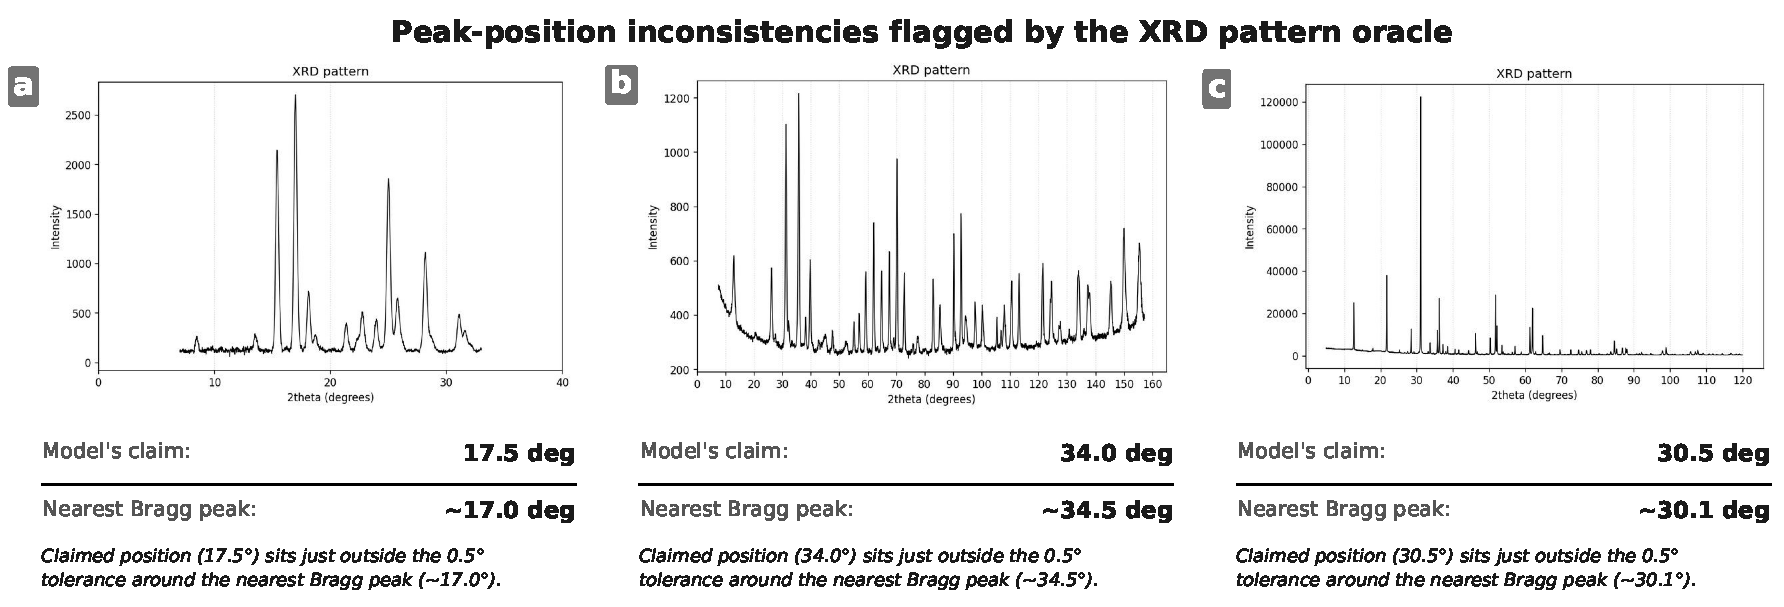
\includegraphics[width=\linewidth]{new_xrd_oracle_figure.pdf}
%\caption{\textbf{Peak-position inconsistencies flagged by the diffraction oracle.} Three
%real, human-confirmed oracle-fired cases: the model's claimed $2\theta$ position, the
%nearest genuine Bragg reflection in the same real diffractogram, and the resulting
%tolerance violation. All three claims sit just outside the oracle's $0.5^\circ$ tolerance
%window around a real peak, consistent with the tolerance-driven false-positive pattern
%described above.}
%\label{fig:xrd-oracle-examples}
%\end{figure}

%\begin{figure}[t]
%\centering
%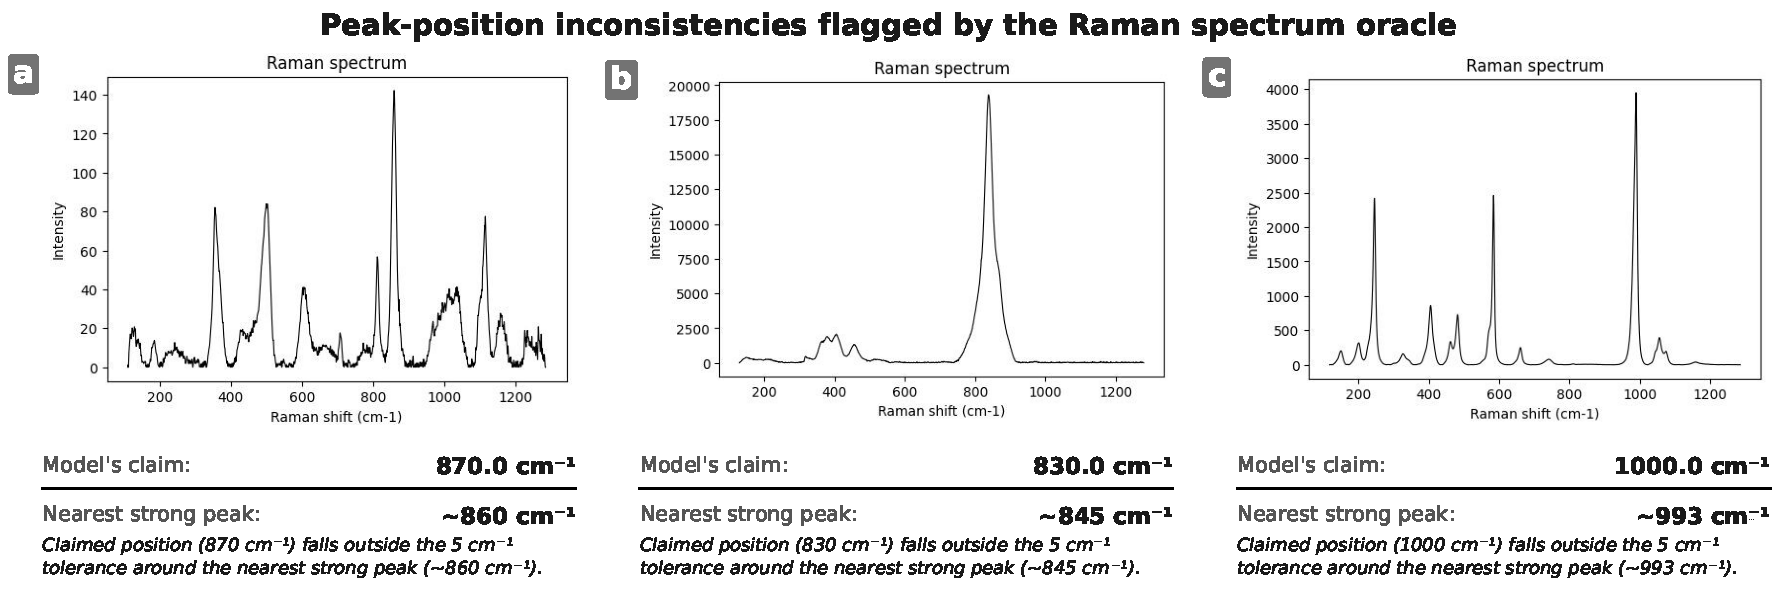
\includegraphics[width=\linewidth]{new_raman_oracle_figure.pdf}
%\caption{\textbf{Peak-position inconsistencies flagged by the Raman spectrum oracle.}
%Three real, human-confirmed oracle-fired cases: the model's claimed Raman shift, the
%nearest genuine strong peak in the same real spectrum, and the resulting tolerance
%violation. All three claims sit just outside the oracle's %$5\,\mathrm{cm}^{-1}$ tolerance
%window around a real peak, the same root cause identified for 34 of 36 %(94\%) of the
%revised spectrum oracle's false positives.}
%\label{fig:raman-oracle-examples}
%\end{figure}

%\begin{figure}[t]
%\centering
%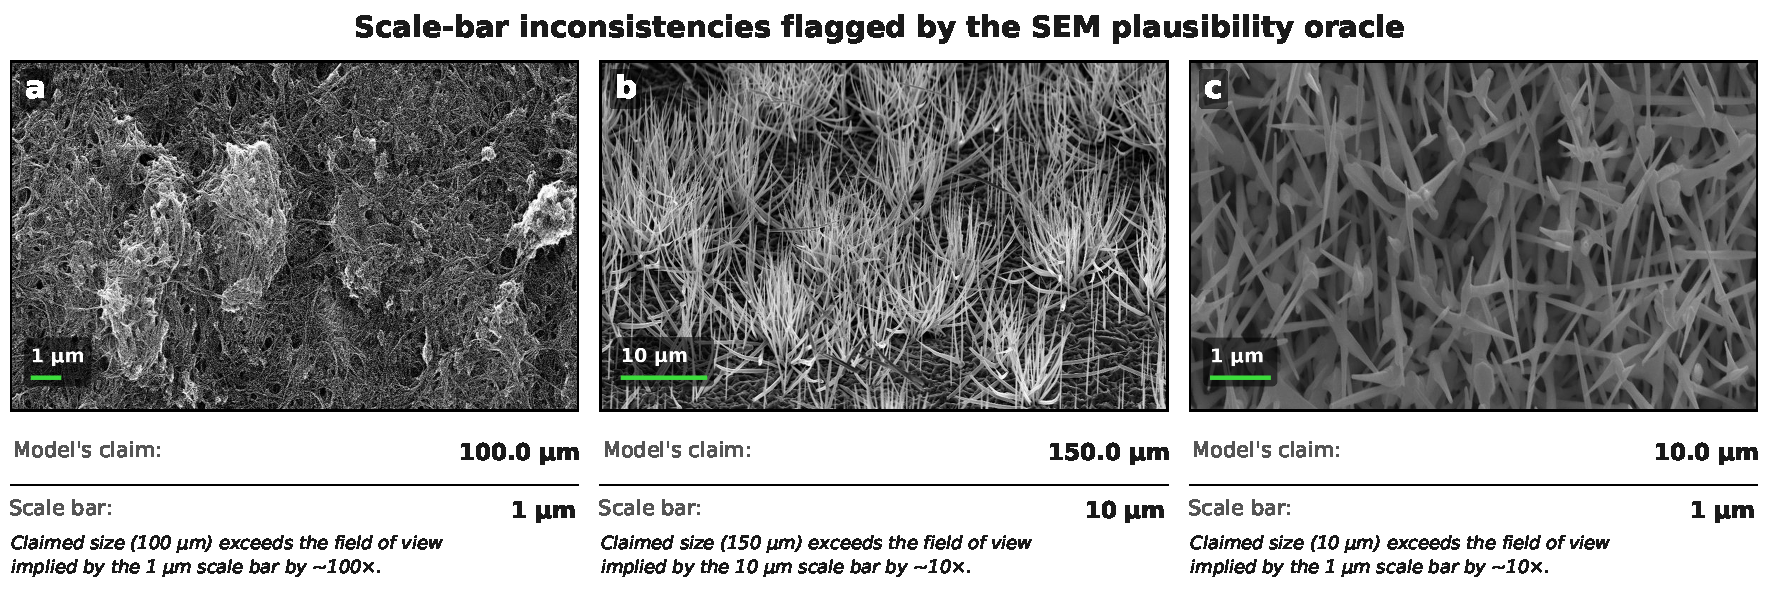
\includegraphics[width=\linewidth]{new_sem_oracle_figure.pdf}
%\caption{\textbf{Scale-bar inconsistencies flagged by the microscopy oracle.} Three real,
%human-confirmed oracle-fired cases: the model's claimed feature size against the real,
%burned-in scale bar of the same NFFA-EUROPE micrograph. Claimed sizes exceed the field of
%view the scale bar implies by roughly $10$--$100\times$, consistent with the scale-bar
%unit and scale-factor arithmetic errors that dominate the microscopy violation taxonomy
%(Results).}
%\label{fig:sem-oracle-examples}
%\end{figure}



\begin{figure}[!htbp]
    \centering

    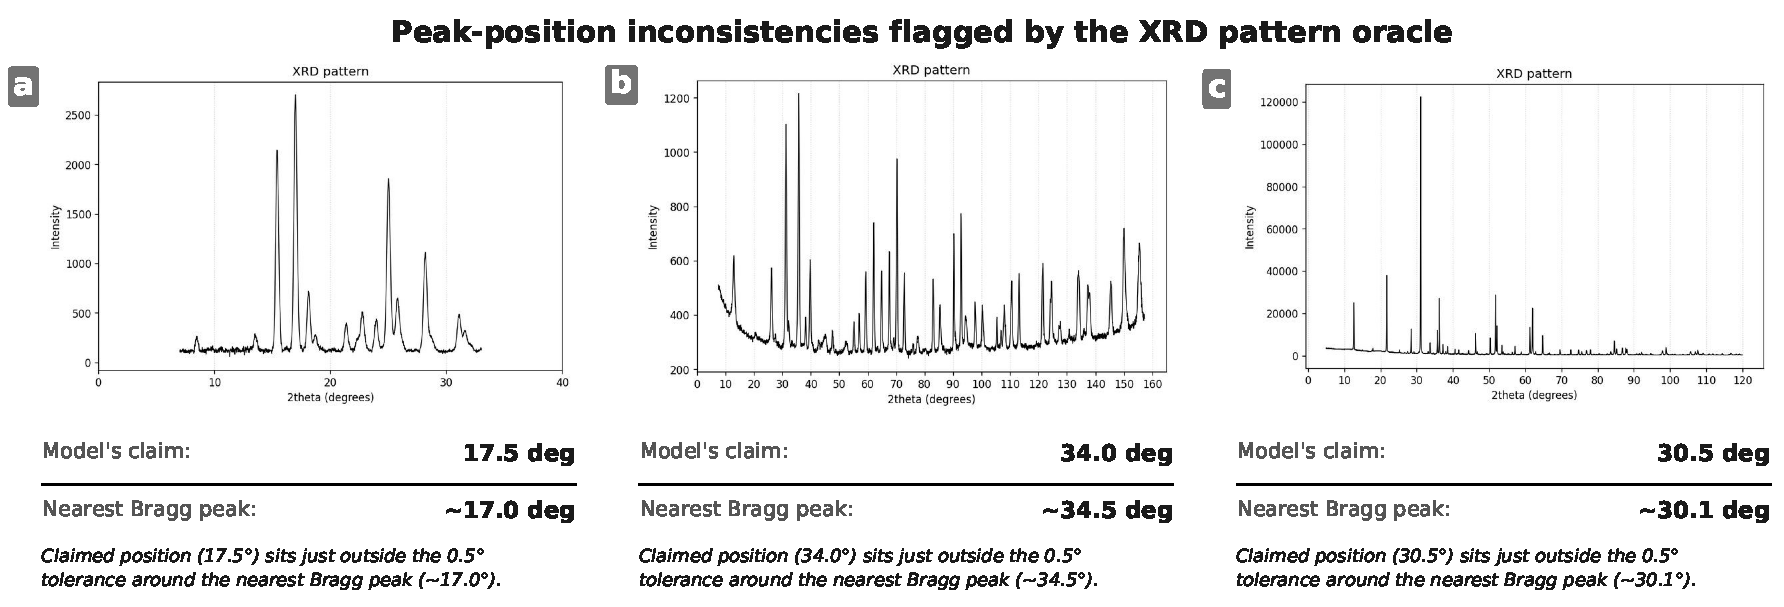
\includegraphics[width=\linewidth,height=0.235\textheight,keepaspectratio]
    {new_xrd_oracle_figure.pdf}

    \vspace{1mm}

    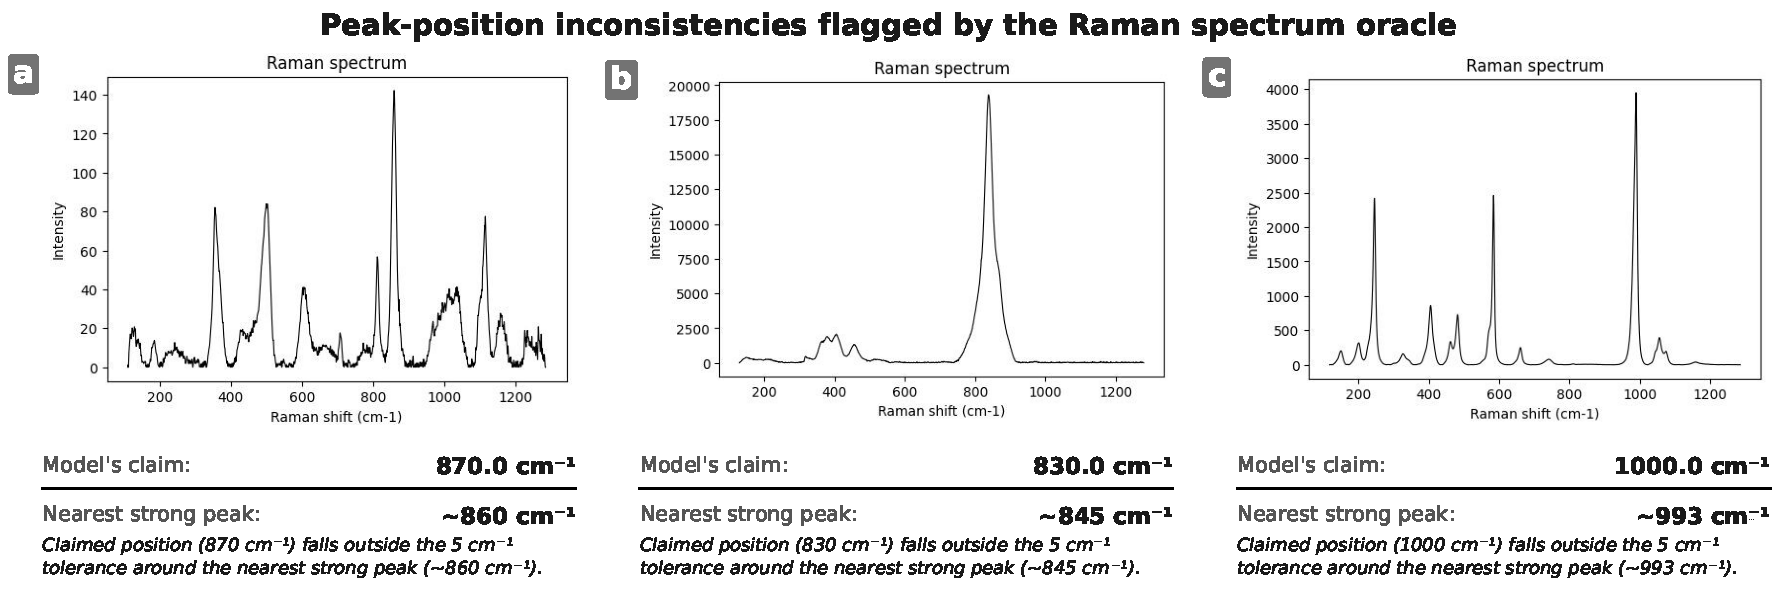
\includegraphics[width=\linewidth,height=0.235\textheight,keepaspectratio]
    {new_raman_oracle_figure.pdf}

    \vspace{1mm}

    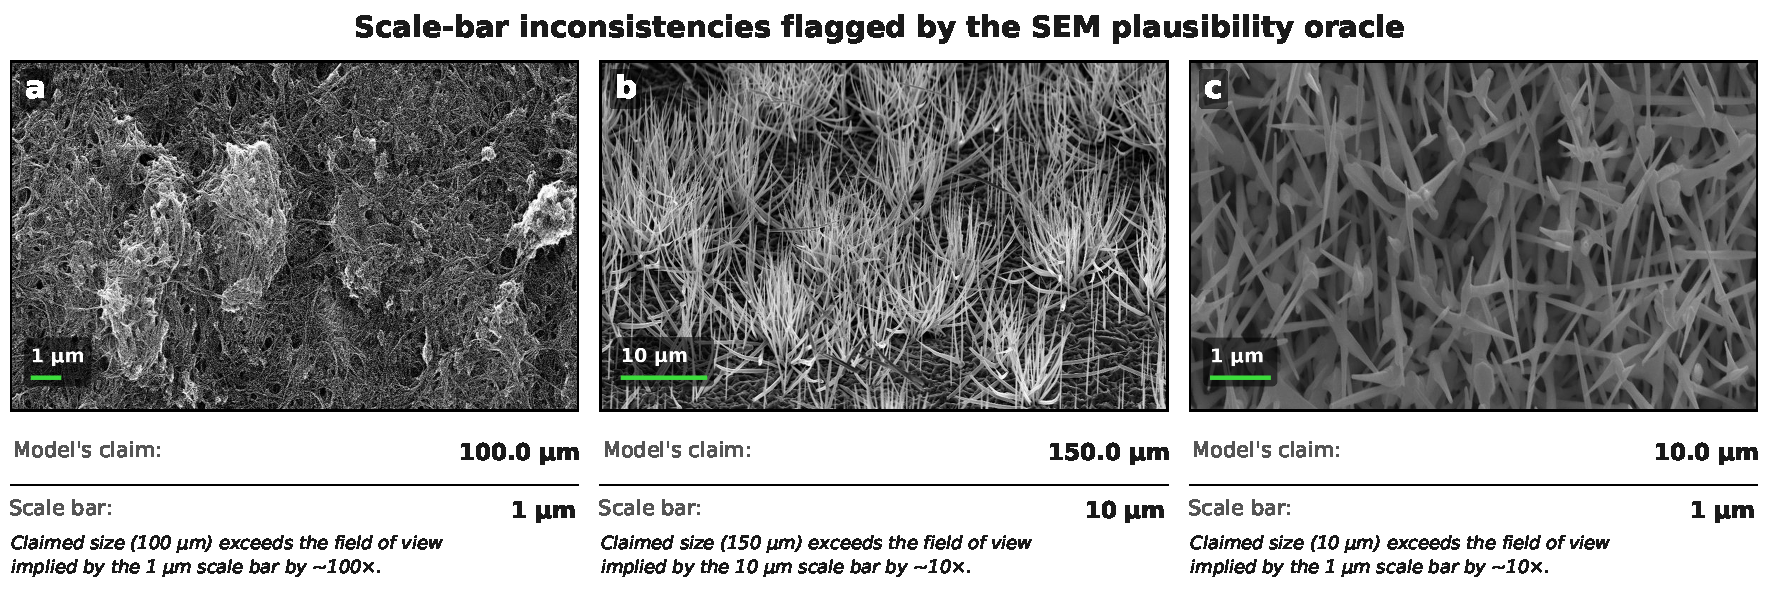
\includegraphics[width=\linewidth,height=0.235\textheight,keepaspectratio]
    {new_sem_oracle_figure.pdf}

    \caption{\justifying\textbf{Representative inconsistencies identified by the multimodal
    oracles.}
    \textbf{a}, X-ray diffraction cases in which the model-reported
    $2\theta$ position lies outside the $0.5^\circ$ tolerance around the nearest
    genuine Bragg reflection.
    \textbf{b}, Raman spectroscopy cases in which the model-reported Raman shift
    exceeds the $5\,\mathrm{cm}^{-1}$ tolerance relative to the nearest genuine
    spectral peak.
    \textbf{c}, Microscopy cases in which the model-reported feature size is
    inconsistent with the physical scale indicated by the embedded scale bar,
    producing discrepancies of approximately $10$--$100\times$.
    All examples are human-confirmed oracle activations and illustrate
    representative tolerance, unit-conversion, and scale-factor failure modes.}

    \label{fig:oracle-examples}
\end{figure}



\begin{table}[t]
\centering
\caption{\justifying\textbf{Oracle validity and audited precision.} The positive-control
false-negative rate is the maximum across three planted violation rates (10\%, 30\%, and 50\%);
all three rates yielded 0.0000 for every oracle family\rev{, which measures completeness on the
injected violation types only}. Audited precision is the fraction of oracle-fired cases from
Qwen2.5-VL-7B and Gemini 2.5 Flash Lite outputs that human review confirmed as genuine
violations of the stated constraint rather than parsing or oracle artifacts\rev{, with Wilson
95\% intervals; $n$ counts decided cases (2 spectrum cases marked unsure are excluded; counting
them either way gives 92.3--92.7\%). Every audit was sampled and judged under the final oracle
definitions used for all reported results (Methods): spectrum responses were collected once and the fired
set re-scored with the final oracle before the audit, and DFT responses were re-collected under the final
definitions before the audit; the diffraction and microscopy audits were carried out in July 2026 and the others in August 2026. Sources: NFFA, NFFA-EUROPE; MP, Materials Project.
$^{a}$Final stability oracle with the near-hull abstention band: the 50 audited cases with
$0<E_{\mathrm{hull}}\le0.05$ eV\,atom$^{-1}$ are not scored; under the original rule the audit gave 95.3\%
[89.5, 98.0] ($n=107$). Consensus: a second annotator, blind to the first labels, re-labelled a random
subsample of 30 audited cases per family stratified by the first annotator's verdict, and the two annotators
adjudicated together every case on which they disagreed (24 in total); the consensus precision is weighted back
to the audited population by stratum, with 95\% intervals from per-stratum Jeffreys posteriors (30 subsampled
cases per family; $^{b}$14, the subsampled stability cases scored under the final oracle). Agreement statistics and the oracle-silent audit are in Supplementary Table~S8.
The full audits were performed by one annotator (R.K.).}}
\label{tab:exp1}
{\scriptsize\setlength{\tabcolsep}{2.5pt}\renewcommand{\arraystretch}{1.12}
\begin{tabular}{l l S[table-format=1.4] c c}
\toprule
Oracle family & Source & {FN rate} & \multicolumn{2}{c}{Audited precision, \% [95\% CI]} \\
\cmidrule(lr){3-3}\cmidrule(lr){4-5}
& & {\itshape positive control} & {\itshape one annotator ($n$)} & \rev{\itshape two-annotator consensus} \\
\midrule
\multicolumn{5}{l}{\itshape Geometric oracles}\\
Diffraction & opXRD & 0.0000 & 77.2 \rev{[68.1, 84.3]} (101) & \rev{60.2 [44.1, 75.4]} \\
Microscopy & NFFA       & 0.0000 & 88.6 \rev{[81.1, 93.3]} (105) & \rev{88.6 [81.8, 93.9]} \\
Raman spectra & RRUFF & 0.0000 & 92.7 \rev{[90.1, 94.7]} (493) & \rev{60.8 [43.6, 76.3]} \\
\addlinespace
\multicolumn{5}{l}{\itshape DFT-grounded oracles}\\
Stability & MP & 0.0000 & \rev{100 [93.7, 100] (57)$^{a}$} & \rev{100 [84.3, 100]$^{b}$} \\
Metallicity & MP & 0.0000 & 94.7 \rev{[89.0, 97.6]} (114) & \rev{94.7 [86.8, 97.0]} \\
Magnetism & MP & 0.0000 & 92.2 \rev{[85.8, 95.8]} (115) & \rev{91.4 [79.9, 96.5]} \\
\bottomrule
\end{tabular}}
\end{table}

\subsection*{Physical consistency of current models}
We measure the Physical-Consistency Rate and per-constraint-type violation rates for
the four originally evaluated models, four later-generation frontier or open models, and
one flagship-tier addition
across diffraction, microscopy, spectra, and
DFT-grounded constraints, separately for image (VLM) and structure or text (LLM)
inputs (Table~\ref{tab:main}, Fig.~\ref{fig:results}a)\rev{. Each (model, constraint-type) cell
sends 30 items per seed to the model, with $S=3$ seeds (90 items per cell); 4{,}334 of these
responses are scored across the nine models. For the image constraint types all nine models
receive the same items in each seed, so their comparisons are paired; for the DFT constraint
types each model and seed draws its own block of materials, so those comparisons are unpaired.
Not every attempted item can be scored. On diffraction, 64 of the 90 items per cell have a
reference pattern the oracle can use (the rest lack a usable structure); on metallicity, 1--8
items per cell fall in the oracle's abstention band, and on stability 11--19 items per cell are
near-hull materials, which the final stability oracle does not score (Methods). Within the items the oracle can score, the
share of responses that state a checkable quantity (coverage) is at least 0.93 in every cell
except GPT-4o on spectra (0.49; Supplementary Table~S2).} Overall PCR ranges from \rev{0.556
(Qwen3-VL-8B-Instruct) to 0.778 (GPT-5.6-Sol, with GPT-5.6-Terra at 0.777)}; models are
markedly more consistent on microscopy (0.67--1.00) than on spectra (0.07--0.83) or
diffraction (0.47--0.82), and the DFT-grounded column is more tightly clustered
(\rev{0.65--0.76}) than any single geometric constraint\rev{.}

\rev{Because PCR excludes responses that state no checkable quantity, a model could in
principle raise its score by stating less. We therefore also scored every cell under two
alternative conventions: counting a non-checkable response as a violation (penalised) and as
consistent (lenient). The overall ordering of the nine models is nearly unchanged (Kendall
$\tau=0.83$ between the reported and penalised conventions and $1.00$ between the reported and
lenient ones); the main change is GPT-4o, from third to fifth under the penalised
convention, because of its low coverage on spectra (Supplementary Table~S2).}

\rev{We test model differences at the item level rather than by comparing interval overlap:
exact McNemar tests on the paired image-arm items, Fisher exact tests on the unpaired DFT items,
and, for overall PCR, a bootstrap that resamples paired items jointly and DFT items within
model (Methods). Holm correction is applied within each family of comparisons (Supplementary
Table~S3). GPT-5.6-Terra exceeds GPT-4o overall by 0.072 (95\% CI $[0.018,0.125]$, Holm
$p=0.045$). Claude Opus 4.6 versus Claude Sonnet 4.5 ($-0.003$, $[-0.050,0.044]$),
Qwen3-VL-8B-Thinking versus Qwen3-VL-8B-Instruct ($+0.034$, $[-0.016,0.083]$) and
GPT-5.6-Sol versus GPT-5.6-Terra ($+0.002$, $[-0.042,0.046]$) are not significant. With
roughly 500 checkable items per model, the smallest overall difference the design detects with
80\% power is 0.064--0.079 depending on the pair, so these three comparisons exclude only
differences larger than about 0.07; they do not show that the models are equivalent. Across all
36 model pairs, 18 differences in overall PCR survive Holm correction; within single
constraint types the detectable difference is 0.11--0.20, so most per-type rankings are not
resolved. On microscopy, the locally run Qwen2.5-VL-7B is the weakest model (0.667, 95\% CI
$[0.563,0.759]$), and seven of the other eight models exceed it after Holm correction (paired
differences $+0.22$ to $+0.33$), while Qwen3-VL-8B-Instruct ($+0.14$, Holm $p=0.12$) does not.} We do not
know whether the gap reflects genuine scale-bar-reading skill or a difference in how each model handles the
info-bar layout variety in the source micrographs, and do not claim more than the
measured difference. The high absolute microscopy rates should also be read against the
looseness of this oracle, which flags only feature sizes exceeding the field of view (a
necessary, not sufficient, condition), so a near-ceiling rate partly reflects an easily
satisfied check. \rev{Diffraction comparisons in particular should be treated as provisional:
the diffraction ranking changes both when the oracle tolerance is varied and when the prompt is
paraphrased (Methods).}

\rev{The DFT column is also sensitive to class composition. The sampled materials are
imbalanced (for stability, only 3--9 of the 70--79 scored materials per model lie on the hull), so a
model that defaults to the majority answer scores well on pooled PCR. Qwen2.5-VL-7B reaches a pooled
stability PCR of 0.917 but answers none of its 4 on-hull materials consistently, a class-balanced rate
of 0.485, whereas GPT-5.6-Terra has the lowest pooled stability PCR (0.653) but a class-balanced rate of
0.814 (Supplementary Table~S4); with so few on-hull materials per model, these class-balanced rates are
imprecise. The ordering of models on the DFT constraint types therefore depends on whether PCR is pooled
or class-balanced, and we report both. To make the DFT comparisons paired as well, we evaluated the
models on one common item set of 90 materials per DFT constraint type, drawn 45 from each reference
class (Supplementary Table~S6); for stability, 34 of the 45 near-hull draws fall in the band the final
oracle does not score, leaving 56 scored materials (11 on the hull, 45 above it). Eight models are
included; Qwen3-VL-8B-Thinking could not be run because its provider endpoint had been withdrawn by the
time of this analysis, and the locally run Qwen2.5-VL-7B was run on CPU in single precision, because no
GPU with bfloat16 support was available then. On this paired set, restricted to the DFT constraint
types, none of the comparisons stated above is significant: GPT-5.6-Terra versus GPT-4o $+0.021$ (95\% CI
$[-0.042,0.085]$), Claude Opus 4.6 versus Claude Sonnet 4.5 $+0.021$ ($[-0.030,0.072]$) and GPT-5.6-Sol
versus GPT-5.6-Terra $+0.030$ ($[-0.013,0.072]$); 3 of the 28 model pairs differ after Holm correction,
all of them Gemini 2.5 Flash Lite scoring lower. The difference between GPT-5.6-Terra and GPT-4o in the
main evaluation therefore comes from the image constraint types, chiefly spectra. The balanced set also
shows a shared failure that the imbalanced sample hid: every model is far less consistent on
computed-metallic compositions (PCR 0.21--0.40) than on gapped ones (0.84--0.96), that is, models
default to calling a composition non-metallic.}

\begin{table}[t]
\centering
\caption{\justifying Main evaluation: Physical-Consistency Rate by constraint type and overall,
\rev{over the checkable responses among 30 attempted items} per (model, constraint-type) cell per seed, $S=3$ seeds pooled per cell
(bootstrap 95\% CIs omitted from this compact view; see Supplementary Table~S1 for the
full per-cell confidence intervals \rev{and checkable counts, Supplementary Table~S2 for coverage
and alternative conventions, Supplementary Table~S3 for paired, Holm-corrected model comparisons,
and Supplementary Table~S4 for class-balanced DFT rates}, and the Methods for why $\rho_t=1-\mathrm{PCR}$ here). DFT column combines the stability, metallicity,
and magnitude constraint types\rev{; near-hull stability materials are not scored (Methods; the original
rule's values are in Supplementary Table~S7)}.  The first four rows are the
originally evaluated models; the next four are the later-generation refresh
(Methods, Baselines subsection). $^{\ddagger}$GPT-5.6-Sol is OpenAI's flagship tier, added
to test whether it exceeds the balanced-tier GPT-5.6-Terra within the same
generation; \rev{the overall difference is $+0.002$ (95\% CI $[-0.042,0.046]$), not significant, so
the design detects no difference between flagship and balanced tier larger than about 0.07}
(Discussion). \rev{Bold marks the column maximum; it does not imply a significant difference from
the next model.}}
\label{tab:main}
{\scriptsize\setlength{\tabcolsep}{5pt}\renewcommand{\arraystretch}{1.12}
\begin{tabular}{l *{5}{S[table-format=1.3]}}
\toprule
& \multicolumn{5}{c}{Physical-Consistency Rate (higher is more consistent)} \\
\cmidrule(lr){2-6}
Model & {Diffraction} & {Microscopy} & {Spectra} & {DFT$^{*}$} & {All$^{*}$} \\
\midrule
Qwen2.5-VL-7B \textit{(open)} & 0.500 & 0.667 & 0.148 & \rev{0.731} & \rev{0.584} \\
Gemini 2.5 Flash Lite & 0.517 & \bfseries 1.000 & 0.278 & \rev{0.658} & \rev{0.630} \\
GPT-4o                & 0.625 & 0.954 & 0.068 & \rev{0.740} & \rev{0.699} \\
Claude Sonnet 4.5     & 0.547 & 0.977 & 0.189 & \bfseries \rev{0.762} & \rev{0.667} \\
\addlinespace
Claude Opus 4.6            & 0.578 & 0.954 & 0.244 & \rev{0.734} & \rev{0.663} \\
GPT-5.6-Terra              & 0.797 & 0.951 & \bfseries 0.833 & \rev{0.696} & \rev{0.777} \\
Qwen3-VL-8B-Instruct       & 0.468 & 0.802 & 0.133 & \rev{0.649} & \rev{0.556} \\
Qwen3-VL-8B-Thinking       & 0.578 & 0.885 & 0.092 & \rev{0.671} & \rev{0.594} \\
\addlinespace
GPT-5.6-Sol$^{\ddagger}$   & \bfseries 0.820 & 0.915 & 0.764 & \rev{0.727} & \bfseries \rev{0.778} \\
\bottomrule
\end{tabular}}
\end{table}


\subsection*{Accuracy versus consistency}
On three constraint types with a genuine, non-circular accuracy criterion distinct
from the oracle's own tolerance (diffraction: agreement with the single nearest true
peak to $0.1^{\circ}$, versus the oracle's looser $0.5^{\circ}$ tolerance; spectra:
agreement with the nearest real measured peak to $2\,\mathrm{cm}^{-1}$, versus the
oracle's prominence-based check; stability: agreement with the Materials
Project \texttt{is\_stable} label, evaluated separately from the oracle's
operational $0.05\,\mathrm{eV\,atom^{-1}}$ near-hull threshold), we report
accuracy alongside PCR and the four-cell breakdown on the same
\rev{838 scored items} ($n=30$ per (model, constraint-type) cell, $S=3$ seeds\rev{, the four originally evaluated
models; this sample is drawn separately from the main evaluation}). Microscopy is excluded: its
prompt elicits only a feature-size claim, so no non-circular accuracy ground truth is
available without a different prompt design. \rev{On the eight diffraction and spectra cells,
accuracy and PCR disagree on a mean of 23.6\% of items, and on stability they coincide
(Fig.~\ref{fig:pipeline}b,c). Part of the diffraction and spectra disagreement is definitional rather
than evidence of reasoning errors that accuracy misses: the accuracy criteria are deliberately tighter
than the oracle tolerances, so the two scores are expected to differ on items that fall between the two
thresholds. What the comparison does establish is that
the two scores measure different properties of the same response, not that PCR detects errors that
accuracy cannot.} Diffraction is dominated by items
that are wrong by the tight accuracy criterion yet still oracle-consistent (up to 36
of 62 items in one diffraction cell, gap 58.1\%): models are frequently close enough to satisfy the
oracle's looser tolerance while measurably off the exact peak. \rev{On spectra, most responses
are wrong by both criteria, so the two scores disagree on few items} (4.2--11.2\% across models). \rev{On stability the two scores coincide under the final protocol,
and this is informative in itself. The oracle's $0.05\,\mathrm{eV\,atom^{-1}}$ near-hull threshold and
Materials Project's own \texttt{is\_stable} label (true only on the hull) disagree on 571 of 3,000 real
entries (19.0\%), and every one of those is a near-hull material, $0<E_{\mathrm{hull}}\le0.05$. The final
oracle does not score that band (Methods), so outside it the two definitions agree, and the stability gap
of 18.0--27.8\% reported under the original rule came entirely from the near-hull materials. The stability
arm still shows the base-rate confound: Qwen2.5-VL-7B is accurate on 61 of 62 unstable materials but on
none of the 8 stable ones, so its near-ceiling raw accuracy reflects the base rate rather than
discriminative skill. Balanced accuracy (the mean of per-class accuracy) is 0.492 (Qwen2.5-VL-7B), 0.690
(Gemini 2.5 Flash Lite), 0.492 (GPT-4o) and 0.992 (Claude Sonnet 4.5); two of the four models are at
chance once the imbalance is corrected for ($n=65$--73 scored materials per model, 5--8 of them stable).}

\rev{What PCR adds to answer accuracy is therefore not a finer measure of correctness but a
different, label-free property. First, it needs no answer key: it is defined on microscopy and
on net magnetization, where this benchmark has no non-circular accuracy criterion, and on any new
item for which a reference structure, scale bar or computed value exists. Second, it is a floor
rather than a target: a violation is a statement the measurement or the reference calculation
rules out, so a violation is informative about the reasoning that produced it (Fig.~\ref{fig:teaser}c
shows what these violations consist of), whereas an accuracy miss may only reflect reading
precision. Third, because it is a necessary condition, PCR cannot certify that a response is
right; a high PCR with low accuracy, as on diffraction, identifies responses that are physically
admissible but imprecise. We therefore present PCR as a complement to answer accuracy where labels
exist and as a substitute screening signal where they do not, not as a replacement for either.}

\subsection*{Effect of self-verification}
We measure PCR before and after CGSV on identical items and test the change with the
exact paired McNemar test, reporting fixes, regressions, and residual violations
(Table~\ref{tab:cgsv}, Fig.~\ref{fig:results}b), on diffraction and spectra, the two constraint types where
the oracle's feedback is an actionable physical constraint the model can re-examine
without the feedback message itself revealing the answer (a scale-bar violation
message would state the conversion factor outright, and the three DFT claim types are
single-shot binary judgments with no intermediate quantity to reconsider). $n=30$
items per (model, constraint-type) cell, $S=3$ seeds, $K=2$ maximum revision rounds, 545
checkable records in total. \rev{Because Algorithm~\ref{alg:cgsv} stops at the first round in which no
violation remains, an item that is consistent before revision is never revised. The absence of
regressions in consistency ($b=0$ in every cell) therefore follows from the stopping rule; it
confirms the implementation but is not evidence about the model.} CGSV raises PCR for all four models pooled across both
constraint types (Qwen2.5-VL-7B $0.338\!\to\!0.439$, $p=3.1\times10^{-5}$; Gemini 2.5
Flash Lite $0.521\!\to\!0.632$, $p=2.4\times10^{-4}$; GPT-4o
$0.434\!\to\!0.593$, $p=7.6\times10^{-6}$; Claude Sonnet 4.5 $0.373\!\to\!0.639$,
$p=4.6\times10^{-13}$\rev{; all survive Holm correction}).
Residual violations remain in every cell after $K=2$ rounds (roughly 40--90\% of
items \rev{on spectra}), so CGSV reduces but does not eliminate violations.

\rev{Because CGSV is scored by the same oracles that supply its feedback, a rise in PCR alone cannot
show that revised answers are more correct. Every item exposes exactly one checkable claim in
every round, so a gain cannot come from the model dropping the claim. To see what the revisions
achieve, we scored each item's first-round and final-round claim against the same non-circular
accuracy criteria as the accuracy-versus-consistency analysis ($0.1^\circ$ for diffraction,
$2\,\mathrm{cm}^{-1}$ for spectra) and compared them on the same items (Table~\ref{tab:cgsvacc}).
Accuracy is a property the loop never observes, so unlike consistency it can regress. On spectra
($n=293$) accuracy rises from 5.8\% to 9.9\%: 14 items become accurate and 2 cease to be (exact
McNemar $p=0.004$). Of the 244 spectrum items the oracle flagged and the model revised, 48 cleared
the oracle; 11 of these moved to the accurate value and 37 to a value the oracle admits but that
is not within the accuracy tolerance, and the remaining 196 stayed inconsistent.
On diffraction ($n=245$; 7 items whose reference pattern could not be computed are omitted) accuracy
rises from 22.9\% to 28.6\%: 14 items become accurate and none ceases to be (exact McNemar $p=0.0001$).
Of the 79 diffraction items the oracle flagged and the model revised, 41 cleared the oracle; 14 of these
moved to the accurate value and 27 to an admissible but inexact one, and 38 stayed inconsistent. Revisions that clear
the oracle therefore mostly move a claim into the physically admissible region rather than onto the
exact value, while also producing a small but significant net gain in correctness. The evidence
supports this narrower statement, not a claim that CGSV corrects the underlying physics in general.}

\rev{We separately ask whether the gain is}
attributable to the oracle signal specifically, or to extra inference-time compute alone,
with three controls matched to CGSV's items, models, and decoding
(Baselines subsection): unaided self-refinement (the model is told to double-check its
answer with no oracle feedback) shows no significant change (before $0.349$, after $0.339$, $n=542$, $b=34$, $c=29$, $p=0.615$);
generic equal-compute re-prompting (the model is simply asked to reconsider) likewise shows
no significant change (before $0.358$, after $0.342$, $n=562$, $b=24$, $c=15$, $p=0.20$). \rev{Both
controls revise every item, including those already consistent, so their nonzero regression counts
are not comparable with CGSV's structural $b=0$; the comparison that matters is the net change,
which is significant for CGSV and absent for both controls.} Best-of-3 independent resampling gives a
random-pick PCR of $0.363$ and an oracle-oracle upper bound (best of 3) of $0.419$
($n=614$). Both fall below CGSV's oracle-guided after-PCR for every model, though the
margin over the weakest, Qwen2.5-VL-7B at $0.439$, is only $0.02$, and the resampling run
draws its own item sample, so we do not test the difference. \rev{These controls show that the PCR gain
is not reproduced by generic self-reflection or by extra sampling at equal compute; they do not
by themselves show that the gain reflects better physics, which is what the paired correctness
analysis above addresses.}

\begin{table}[t]
\centering
\caption{\justifying Effect of Constraint-Grounded Self-Verification, pooled across diffraction
and spectra, $n=30$ items per (model, constraint-type) cell, $S=3$ seeds, $K=2$ rounds.
$\Delta$: PCR gain (after minus before); $b$: regressions (before-consistent,
after-inconsistent); $c$: fixes (before-inconsistent, after-consistent); $p$: exact
two-sided McNemar test on $(b,c)$; $p_{\mathrm{Holm}}$: Holm-Bonferroni-adjusted $p$ over
this table's 6-test family (Methods, Statistics paragraph). All four CGSV effects survive
this correction; both controls remain non-significant. \rev{For CGSV, $b=0$ follows from the stopping
rule (an item consistent before revision is never revised); the controls revise every item, so
their $b$ is not comparable. Paired changes in correctness are in Table~\ref{tab:cgsvacc}.}}
\label{tab:cgsv}
{\scriptsize\setlength{\tabcolsep}{3.4pt}\renewcommand{\arraystretch}{1.12}
\begin{tabular}{l S[table-format=1.3] S[table-format=1.3] S[table-format=+1.3] S[table-format=2.0] S[table-format=2.0] c c}
\toprule
& \multicolumn{3}{c}{PCR} & \multicolumn{2}{c}{Discordant} & & \\
\cmidrule(lr){2-4}\cmidrule(lr){5-6}
Model & {before} & {after} & {$\Delta$} & {$b$} & {$c$} & {$p$} & {$p_{\mathrm{Holm}}$} \\
\midrule
Qwen2.5-VL-7B         & 0.338 & 0.439 & 0.101 & 0 & 16 & $3.1\times10^{-5}$ & $1.2\times10^{-4}$ \\
Gemini 2.5 Flash Lite & 0.521 & 0.632 & 0.111 & 0 & 13 & $2.4\times10^{-4}$ & $7.3\times10^{-4}$ \\
GPT-4o                & 0.434 & 0.593 & \bfseries 0.159 & 0 & 18 & $7.6\times10^{-6}$ & $3.8\times10^{-5}$ \\
Claude Sonnet 4.5     & 0.373 & 0.639 & \bfseries 0.266 & 0 & 42 & $4.6\times10^{-13}$ & $2.7\times10^{-12}$ \\
\midrule
\multicolumn{8}{l}{\itshape Mechanism-isolation controls (pooled across models, both constraint types)}\\
Self-refinement (no oracle) & 0.349 & 0.339 & -0.010 & 34 & 29 & 0.615 & 0.615 \\
Generic re-prompting        & 0.358 & 0.342 & -0.016 & 24 & 15 & 0.20 & 0.399 \\
\bottomrule
\end{tabular}}
\end{table}

\begin{table}[t]
\revon\centering
\caption{\justifying Paired change in answer correctness before and after CGSV, on the same items as
Table~\ref{tab:cgsv}. Accuracy uses the non-circular criteria of the accuracy-versus-consistency
analysis (diffraction: within $0.1^\circ$ of the nearest reference reflection; spectra: within
$2\,\mathrm{cm}^{-1}$ of the nearest detected local maximum), applied to each item's first-round
and final-round claim (accuracy before$\to$after). L/G: items that stop (lost) or start (gained) being
accurate; $p$: exact two-sided McNemar test on (L, G). Rev.: items the oracle flagged at round 1 and the
model revised; of these, A cleared the oracle with an accurate value, Ad cleared it with an admissible
value outside the accuracy tolerance, and U were still flagged after $K=2$ rounds.}
\label{tab:cgsvacc}
{\scriptsize\setlength{\tabcolsep}{2.5pt}\renewcommand{\arraystretch}{1.12}
\begin{tabular}{l l r c c r r c}
\toprule
Constraint & Model & $n$ & Accuracy & L/G & $p$ & Rev. & A/Ad/U \\
\midrule
Spectra & Qwen2.5-VL-7B & 89 & 0.067$\to$0.101 & 0/3 & 0.25 & 80 & 3/9/68 \\
 & Gemini 2.5 F.\ Lite & 69 & 0.043$\to$0.072 & 0/2 & 0.50 & 49 & 2/6/41 \\
 & GPT-4o & 45 & 0.044$\to$0.044 & 1/1 & 1.00 & 40 & 0/4/36 \\
 & Claude Sonnet 4.5 & 90 & 0.067$\to$0.144 & 1/8 & 0.039 & 75 & 6/18/51 \\
 & \textit{pooled} & 293 & 0.058$\to$0.099 & 2/14 & 0.004 & 244 & 11/37/196 \\
\addlinespace
Diffraction & Qwen2.5-VL-7B & 66 & 0.303$\to$0.318 & 0/1 & 1.00 & 24 & 1/3/20 \\
 & Gemini 2.5 F.\ Lite & 47 & 0.213$\to$0.255 & 0/2 & 0.50 & 7 & 2/3/2 \\
 & GPT-4o & 66 & 0.152$\to$0.212 & 0/4 & 0.12 & 24 & 4/10/10 \\
 & Claude Sonnet 4.5 & 66 & 0.242$\to$0.348 & 0/7 & 0.016 & 24 & 7/11/6 \\
 & \textit{pooled} & 245 & 0.229$\to$0.286 & 0/14 & 0.0001 & 79 & 14/27/38 \\
\bottomrule
\end{tabular}}
\end{table}

\subsection*{Verifier for violation prediction}
We fine-tune Qwen2.5-0.5B-Instruct with LoRA on oracle-derived labels alone (no human
annotation) to predict, from the input description and chain text alone, whether a
physical violation is present, using 2{,}152 real oracle-checked records spanning all
six constraint types collected across the preceding evaluations. We report precision,
recall, $F_1$, ROC AUC, and expected calibration error (ECE) on an 80/20
in-distribution split and separately on six held-out-constraint-type splits (train on the
other five constraint types, test on one entirely unseen one). The in-distribution split
is disjoint at the parent source (item or structure) level, \rev{so no source item contributes
records to both sides}. In distribution the verifier is a useful
detector overall (precision 0.77, recall 0.71, $F_1=0.74$, AUC $=0.850$, ECE $=0.096$).
\rev{This pooled figure overstates its usefulness for a given scientific task, for two reasons.
First, the six families have very different violation base rates (19\% for microscopy to 88\%
for spectra in the test split), so a score that only identified the family would already rank
violations above chance: a baseline that assigns each item its family's training-set violation
rate reaches AUC $=0.759$. Second, within single families the verifier's discrimination varies
widely (Table~\ref{tab:verifierfam}): it is strong on microscopy (AUC $0.922$, 95\% CI
$[0.852,0.977]$) and stability ($0.804$, $[0.683,0.903]$), moderate on magnetism ($0.728$,
$[0.562,0.877]$) and diffraction ($0.696$, $[0.493,0.895]$), and not distinguishable from chance on
metallicity ($0.582$, $[0.390,0.775]$) and spectra ($0.513$, $[0.353,0.702]$). The in-distribution
verifier is therefore a useful triage signal for microscopy and stability claims, a weak one for
magnetism and diffraction, and not useful for metallicity or spectra.} Its
cross-constraint-type generalization is poor for all six constraint types: diffraction, microscopy, and stability
are indistinguishable from chance when held out entirely (AUC 0.50, 0.53, and 0.44,
bootstrap 95\% confidence intervals straddling 0.5), spectra is not separable from chance either (AUC
0.56, CI $[0.488,0.626]$)\rev{, magnetism is at chance (AUC $0.503$, $[0.430,0.576]$),} and metallicity is the single arguable exception, with a nominal
95\% interval that excludes chance (AUC 0.58, CI $[0.510,0.652]$) but that no longer does so
once the interval is widened for the six held-out comparisons (Bonferroni-corrected interval
$[0.487,0.673]$). We therefore treat metallicity as a nominal, uncorrected exception rather
than as evidence of transfer, and do not build any claim on it. \rev{No held-out constraint type shows transfer that survives correction for the six comparisons.} We report the verifier as an
in-distribution tool \rev{for the families where it discriminates}, and explicitly do \emph{not} claim it as a general-purpose,
constraint-agnostic violation detector. A pooled AUC across all six held-out constraint
types is not reported: the six held-out runs are separately fine-tuned models, so their raw
probability outputs are not on a directly comparable scale; we report only the six
per-constraint-type numbers (Table~\ref{tab:verifier}, Fig.~\ref{fig:results}c). \rev{The held-out results are sensitive to the training run. The released adapters, retrained
with the same data, splits and seed but in a different numerical precision (Supplementary Note~2),
reproduce the in-distribution AUC exactly ($0.850$) but move the held-out AUCs by up to $0.08$: held-out
microscopy rises to $0.602$, whose interval excludes chance even after Bonferroni correction
($[0.519,0.682]$), and held-out stability falls to $0.383$, below chance. No held-out family reaches a
level useful for triage in either run, which is the conclusion we draw. The verifier was trained on
oracle labels produced under the original stability rule; evaluated only on the test items that the final
oracle scores, its in-distribution AUC is $0.871$ ($[0.834,0.904]$; stability family $0.911$) and its
held-out stability AUC $0.372$, so the conclusions above do not depend on the near-hull band
(Supplementary Note~2).}

\begin{table}[t]
\centering
\caption{\justifying Verifier precision/recall/$F_1$ (in-distribution and held-out-constraint-type
splits, both source-disjoint) and the detector's bootstrap 95\% CI on ROC AUC, predicting a
real oracle violation from held-out verifier scores. Expected calibration error is
reported in the text for the in-distribution split (ECE $=0.096$). No pooled
across-constraint-type AUC is reported (see text).}
\label{tab:verifier}
{\scriptsize\setlength{\tabcolsep}{5pt}\renewcommand{\arraystretch}{1.12}
\begin{tabular}{l S[table-format=1.3] S[table-format=1.3] S[table-format=1.3] S[table-format=1.3] c}
\toprule
& \multicolumn{3}{c}{Violation prediction} & \multicolumn{2}{c}{Detector (ROC)} \\
\cmidrule(lr){2-4}\cmidrule(lr){5-6}
Split & {Precision} & {Recall} & {$F_1$} & {AUC} & {95\% CI} \\
\midrule
\multicolumn{6}{l}{\itshape In distribution (80/20 split, source-disjoint)}\\
All constraint types & 0.768 & 0.706 & 0.735 & \bfseries 0.850 & {[}0.813, 0.883{]} \\
\addlinespace
\multicolumn{6}{l}{\itshape Held out entirely (train on the other five constraint types)}\\
Diffraction (XRD)      & 0.600 & 0.030 & 0.057 & 0.497 & {[}0.419, 0.578{]} \\
Microscopy (SEM)       & 0.239 & 0.905 & 0.378 & 0.527 & {[}0.468, 0.589{]} \\
Spectra (Raman)        & {--} & 0.000 & {--} & 0.558 & {[}0.488, 0.626{]} \\
Stability$^{*}$        & 0.355 & 0.103 & 0.159 & 0.436 & {[}0.370, 0.502{]} \\
Metallicity$^{*}$      & 0.486 & 0.158 & 0.238 & 0.582 & {[}0.510, 0.652{]} \\
Magnetism$^{*}$        & 0.468 & 0.635 & 0.539 & 0.503 & {[}0.430, 0.576{]} \\
\bottomrule
\end{tabular}}
\end{table}

\begin{table}[t]
\revon\centering
\caption{\justifying In-distribution verifier performance within each constraint family (the
source-disjoint 80/20 test split of Table~\ref{tab:verifier}, broken down by family; scores are those of
the single in-distribution model). AUC 95\% CI: bootstrap over source items ($B=5000$).
Viol.: share of test records that are oracle violations. A baseline that scores each record by
its family's training-set violation rate reaches a pooled AUC of 0.759, against the verifier's
0.850. Labels follow the original stability rule; on the items the final rule scores, the stability AUC is
0.911 (Supplementary Note~2).}
\label{tab:verifierfam}
{\scriptsize\setlength{\tabcolsep}{5pt}\renewcommand{\arraystretch}{1.12}
\begin{tabular}{l r r S[table-format=1.3] S[table-format=1.3] S[table-format=1.3] S[table-format=1.3] c}
\toprule
Family & $n$ & {Viol.} & {Precision} & {Recall} & {$F_1$} & {AUC} & {95\% CI} \\
\midrule
Diffraction (XRD)  & 33  & 70\% & 0.846 & 0.478 & 0.611 & 0.696 & {[}0.493, 0.895{]} \\
Microscopy (SEM)   & 109 & 19\% & 0.750 & 0.714 & 0.732 & 0.922 & {[}0.852, 0.977{]} \\
Spectra (Raman)    & 100 & 88\% & 0.880 & 1.000 & 0.936 & 0.513 & {[}0.353, 0.702{]} \\
Stability$^{*}$    & 87  & 31\% & 0.727 & 0.296 & 0.421 & 0.804 & {[}0.683, 0.903{]} \\
Metallicity$^{*}$  & 55  & 35\% & 0.364 & 0.421 & 0.390 & 0.582 & {[}0.390, 0.775{]} \\
Magnetism$^{*}$    & 47  & 40\% & 0.600 & 0.474 & 0.529 & 0.728 & {[}0.562, 0.877{]} \\
\bottomrule
\end{tabular}}
\end{table}

% Figure: main results (heatmap + slopegraph + forest)
\begin{figure}[p]
\centering
\resizebox{0.975\linewidth}{!}{%
\begin{tikzpicture}[font=\sffamily]
\node[plab,anchor=west] at (-0.10,7.62){a)};
\node[font=\sffamily\small\bfseries,anchor=west] at (0.55,7.62){Physical consistency by model and constraint type};
\draw[black!45,line width=0.5pt](2.57,7.10)--(6.89,7.10);
\draw[black!45,line width=0.5pt](6.92,7.10)--(11.24,7.10);
\node[font=\sffamily\fontsize{6.5}{8}\selectfont,black!60,anchor=south] at (4.73,7.14){geometric oracles};
\node[font=\sffamily\fontsize{6.5}{8}\selectfont,black!60,anchor=south] at (9.08,7.14){DFT-grounded oracles};
\node[font=\sffamily\fontsize{6.8}{8}\selectfont,anchor=south] at (3.28,6.60){Diffraction};
\node[font=\sffamily\fontsize{6}{7}\selectfont,black!55,anchor=south] at (3.28,6.30){(XRD)};
\node[font=\sffamily\fontsize{6.8}{8}\selectfont,anchor=south] at (4.73,6.60){Microscopy};
\node[font=\sffamily\fontsize{6}{7}\selectfont,black!55,anchor=south] at (4.73,6.30){(SEM)};
\node[font=\sffamily\fontsize{6.8}{8}\selectfont,anchor=south] at (6.18,6.60){Spectra};
\node[font=\sffamily\fontsize{6}{7}\selectfont,black!55,anchor=south] at (6.18,6.30){(Raman)};
\node[font=\sffamily\fontsize{6.8}{8}\selectfont,anchor=south] at (7.63,6.60){Stability};
\node[font=\sffamily\fontsize{6}{7}\selectfont,black!55,anchor=south] at (7.63,6.30){$^{*}$};
\node[font=\sffamily\fontsize{6.8}{8}\selectfont,anchor=south] at (9.08,6.60){Metallicity};
\node[font=\sffamily\fontsize{6}{7}\selectfont,black!55,anchor=south] at (9.08,6.30){$^{*}$};
\node[font=\sffamily\fontsize{6.8}{8}\selectfont,anchor=south] at (10.53,6.60){Magnetism};
\node[font=\sffamily\fontsize{6}{7}\selectfont,black!55,anchor=south] at (10.53,6.30){$^{*}$};
\node[font=\sffamily\fontsize{6.8}{8}\selectfont\bfseries,anchor=south] at (12.36,6.60){Overall};
\node[font=\sffamily\fontsize{6}{7}\selectfont,black!55,anchor=south] at (12.36,6.30){(all six)};
\node[font=\sffamily\fontsize{6.8}{8}\selectfont,anchor=east] at (2.45,5.23){GPT-5.6-Terra$^{\dagger}$};
\node[minimum width=1.42cm,minimum height=0.56cm,fill=npblue!71,draw=white,line width=1pt,inner sep=0,font=\sffamily\fontsize{7.2}{8}\selectfont,text=white] at (3.28,5.23){0.797};
\node[minimum width=1.42cm,minimum height=0.56cm,fill=npblue!84,draw=white,line width=1pt,inner sep=0,font=\sffamily\fontsize{7.2}{8}\selectfont,text=white] at (4.73,5.23){0.951};
\node[minimum width=1.42cm,minimum height=0.56cm,fill=npblue!74,draw=white,line width=1pt,inner sep=0,font=\sffamily\fontsize{7.2}{8}\selectfont,text=white] at (6.18,5.23){0.833};
\node[minimum width=1.42cm,minimum height=0.56cm,fill=npblue!60,draw=white,line width=1pt,inner sep=0,font=\sffamily\fontsize{7.2}{8}\selectfont,text=white] at (7.63,5.23){0.653};
\node[minimum width=1.42cm,minimum height=0.56cm,fill=npblue!60,draw=white,line width=1pt,inner sep=0,font=\sffamily\fontsize{7.2}{8}\selectfont,text=white] at (9.08,5.23){0.659};
\node[minimum width=1.42cm,minimum height=0.56cm,fill=npblue!69,draw=white,line width=1pt,inner sep=0,font=\sffamily\fontsize{7.2}{8}\selectfont,text=white] at (10.53,5.23){0.767};
\node[minimum width=1.42cm,minimum height=0.56cm,fill=npblue!70,draw=black!45,line width=0.6pt,inner sep=0,font=\sffamily\fontsize{7.2}{8}\selectfont\bfseries,text=white] at (12.36,5.23){0.777};
\node[font=\sffamily\fontsize{6.8}{8}\selectfont,anchor=east] at (2.45,5.85){GPT-5.6-Sol$^{\ddagger}$};
\node[minimum width=1.42cm,minimum height=0.56cm,fill=npblue!73,draw=white,line width=1pt,inner sep=0,font=\sffamily\fontsize{7.2}{8}\selectfont,text=white] at (3.28,5.85){0.820};
\node[minimum width=1.42cm,minimum height=0.56cm,fill=npblue!81,draw=white,line width=1pt,inner sep=0,font=\sffamily\fontsize{7.2}{8}\selectfont,text=white] at (4.73,5.85){0.915};
\node[minimum width=1.42cm,minimum height=0.56cm,fill=npblue!69,draw=white,line width=1pt,inner sep=0,font=\sffamily\fontsize{7.2}{8}\selectfont,text=white] at (6.18,5.85){0.764};
\node[minimum width=1.42cm,minimum height=0.56cm,fill=npblue!71,draw=white,line width=1pt,inner sep=0,font=\sffamily\fontsize{7.2}{8}\selectfont,text=white] at (7.63,5.85){0.789};
\node[minimum width=1.42cm,minimum height=0.56cm,fill=npblue!61,draw=white,line width=1pt,inner sep=0,font=\sffamily\fontsize{7.2}{8}\selectfont,text=white] at (9.08,5.85){0.670};
\node[minimum width=1.42cm,minimum height=0.56cm,fill=npblue!66,draw=white,line width=1pt,inner sep=0,font=\sffamily\fontsize{7.2}{8}\selectfont,text=white] at (10.53,5.85){0.733};
\node[minimum width=1.42cm,minimum height=0.56cm,fill=npblue!70,draw=black!45,line width=0.6pt,inner sep=0,font=\sffamily\fontsize{7.2}{8}\selectfont\bfseries,text=white] at (12.36,5.85){0.778};
\node[font=\sffamily\fontsize{6.8}{8}\selectfont,anchor=east] at (2.45,4.62){GPT-4o};
\node[minimum width=1.42cm,minimum height=0.56cm,fill=npblue!57,draw=white,line width=1pt,inner sep=0,font=\sffamily\fontsize{7.2}{8}\selectfont,text=black] at (3.28,4.62){0.625};
\node[minimum width=1.42cm,minimum height=0.56cm,fill=npblue!84,draw=white,line width=1pt,inner sep=0,font=\sffamily\fontsize{7.2}{8}\selectfont,text=white] at (4.73,4.62){0.954};
\node[minimum width=1.42cm,minimum height=0.56cm,fill=npblue!12,draw=white,line width=1pt,inner sep=0,font=\sffamily\fontsize{7.2}{8}\selectfont,text=black] at (6.18,4.62){0.068};
\node[minimum width=1.42cm,minimum height=0.56cm,fill=npblue!79,draw=white,line width=1pt,inner sep=0,font=\sffamily\fontsize{7.2}{8}\selectfont,text=white] at (7.63,4.62){0.886};
\node[minimum width=1.42cm,minimum height=0.56cm,fill=npblue!61,draw=white,line width=1pt,inner sep=0,font=\sffamily\fontsize{7.2}{8}\selectfont,text=white] at (9.08,4.62){0.671};
\node[minimum width=1.42cm,minimum height=0.56cm,fill=npblue!62,draw=white,line width=1pt,inner sep=0,font=\sffamily\fontsize{7.2}{8}\selectfont,text=white] at (10.53,4.62){0.678};
\node[minimum width=1.42cm,minimum height=0.56cm,fill=npblue!63,draw=black!45,line width=0.6pt,inner sep=0,font=\sffamily\fontsize{7.2}{8}\selectfont\bfseries,text=white] at (12.36,4.62){0.699};
\node[font=\sffamily\fontsize{6.8}{8}\selectfont,anchor=east] at (2.45,4.00){Claude Sonnet 4.5};
\node[minimum width=1.42cm,minimum height=0.56cm,fill=npblue!51,draw=white,line width=1pt,inner sep=0,font=\sffamily\fontsize{7.2}{8}\selectfont,text=black] at (3.28,4.00){0.547};
\node[minimum width=1.42cm,minimum height=0.56cm,fill=npblue!86,draw=white,line width=1pt,inner sep=0,font=\sffamily\fontsize{7.2}{8}\selectfont,text=white] at (4.73,4.00){0.977};
\node[minimum width=1.42cm,minimum height=0.56cm,fill=npblue!21,draw=white,line width=1pt,inner sep=0,font=\sffamily\fontsize{7.2}{8}\selectfont,text=black] at (6.18,4.00){0.189};
\node[minimum width=1.42cm,minimum height=0.56cm,fill=npblue!76,draw=white,line width=1pt,inner sep=0,font=\sffamily\fontsize{7.2}{8}\selectfont,text=white] at (7.63,4.00){0.849};
\node[minimum width=1.42cm,minimum height=0.56cm,fill=npblue!63,draw=white,line width=1pt,inner sep=0,font=\sffamily\fontsize{7.2}{8}\selectfont,text=white] at (9.08,4.00){0.694};
\node[minimum width=1.42cm,minimum height=0.56cm,fill=npblue!68,draw=white,line width=1pt,inner sep=0,font=\sffamily\fontsize{7.2}{8}\selectfont,text=white] at (10.53,4.00){0.756};
\node[minimum width=1.42cm,minimum height=0.56cm,fill=npblue!61,draw=black!45,line width=0.6pt,inner sep=0,font=\sffamily\fontsize{7.2}{8}\selectfont\bfseries,text=white] at (12.36,4.00){0.667};
\node[font=\sffamily\fontsize{6.8}{8}\selectfont,anchor=east] at (2.45,3.39){Claude Opus 4.6$^{\dagger}$};
\node[minimum width=1.42cm,minimum height=0.56cm,fill=npblue!53,draw=white,line width=1pt,inner sep=0,font=\sffamily\fontsize{7.2}{8}\selectfont,text=black] at (3.28,3.39){0.578};
\node[minimum width=1.42cm,minimum height=0.56cm,fill=npblue!84,draw=white,line width=1pt,inner sep=0,font=\sffamily\fontsize{7.2}{8}\selectfont,text=white] at (4.73,3.39){0.954};
\node[minimum width=1.42cm,minimum height=0.56cm,fill=npblue!26,draw=white,line width=1pt,inner sep=0,font=\sffamily\fontsize{7.2}{8}\selectfont,text=black] at (6.18,3.39){0.244};
\node[minimum width=1.42cm,minimum height=0.56cm,fill=npblue!71,draw=white,line width=1pt,inner sep=0,font=\sffamily\fontsize{7.2}{8}\selectfont,text=white] at (7.63,3.39){0.789};
\node[minimum width=1.42cm,minimum height=0.56cm,fill=npblue!65,draw=white,line width=1pt,inner sep=0,font=\sffamily\fontsize{7.2}{8}\selectfont,text=white] at (9.08,3.39){0.721};
\node[minimum width=1.42cm,minimum height=0.56cm,fill=npblue!63,draw=white,line width=1pt,inner sep=0,font=\sffamily\fontsize{7.2}{8}\selectfont,text=white] at (10.53,3.39){0.700};
\node[minimum width=1.42cm,minimum height=0.56cm,fill=npblue!60,draw=black!45,line width=0.6pt,inner sep=0,font=\sffamily\fontsize{7.2}{8}\selectfont\bfseries,text=white] at (12.36,3.39){0.663};
\node[font=\sffamily\fontsize{6.8}{8}\selectfont,anchor=east] at (2.45,2.77){Gemini 2.5 Flash Lite};
\node[minimum width=1.42cm,minimum height=0.56cm,fill=npblue!48,draw=white,line width=1pt,inner sep=0,font=\sffamily\fontsize{7.2}{8}\selectfont,text=black] at (3.28,2.77){0.517};
\node[minimum width=1.42cm,minimum height=0.56cm,fill=npblue!88,draw=white,line width=1pt,inner sep=0,font=\sffamily\fontsize{7.2}{8}\selectfont,text=white] at (4.73,2.77){1.000};
\node[minimum width=1.42cm,minimum height=0.56cm,fill=npblue!29,draw=white,line width=1pt,inner sep=0,font=\sffamily\fontsize{7.2}{8}\selectfont,text=black] at (6.18,2.77){0.278};
\node[minimum width=1.42cm,minimum height=0.56cm,fill=npblue!73,draw=white,line width=1pt,inner sep=0,font=\sffamily\fontsize{7.2}{8}\selectfont,text=white] at (7.63,2.77){0.814};
\node[minimum width=1.42cm,minimum height=0.56cm,fill=npblue!64,draw=white,line width=1pt,inner sep=0,font=\sffamily\fontsize{7.2}{8}\selectfont,text=white] at (9.08,2.77){0.702};
\node[minimum width=1.42cm,minimum height=0.56cm,fill=npblue!47,draw=white,line width=1pt,inner sep=0,font=\sffamily\fontsize{7.2}{8}\selectfont,text=black] at (10.53,2.77){0.494};
\node[minimum width=1.42cm,minimum height=0.56cm,fill=npblue!58,draw=black!45,line width=0.6pt,inner sep=0,font=\sffamily\fontsize{7.2}{8}\selectfont\bfseries,text=black] at (12.36,2.77){0.630};
\node[font=\sffamily\fontsize{6.8}{8}\selectfont,anchor=east] at (2.45,2.16){Qwen3-VL-8B-Thinking$^{\dagger}$};
\node[minimum width=1.42cm,minimum height=0.56cm,fill=npblue!53,draw=white,line width=1pt,inner sep=0,font=\sffamily\fontsize{7.2}{8}\selectfont,text=black] at (3.28,2.16){0.578};
\node[minimum width=1.42cm,minimum height=0.56cm,fill=npblue!79,draw=white,line width=1pt,inner sep=0,font=\sffamily\fontsize{7.2}{8}\selectfont,text=white] at (4.73,2.16){0.885};
\node[minimum width=1.42cm,minimum height=0.56cm,fill=npblue!14,draw=white,line width=1pt,inner sep=0,font=\sffamily\fontsize{7.2}{8}\selectfont,text=black] at (6.18,2.16){0.092};
\node[minimum width=1.42cm,minimum height=0.56cm,fill=npblue!79,draw=white,line width=1pt,inner sep=0,font=\sffamily\fontsize{7.2}{8}\selectfont,text=white] at (7.63,2.16){0.895};
\node[minimum width=1.42cm,minimum height=0.56cm,fill=npblue!59,draw=white,line width=1pt,inner sep=0,font=\sffamily\fontsize{7.2}{8}\selectfont,text=black] at (9.08,2.16){0.644};
\node[minimum width=1.42cm,minimum height=0.56cm,fill=npblue!47,draw=white,line width=1pt,inner sep=0,font=\sffamily\fontsize{7.2}{8}\selectfont,text=black] at (10.53,2.16){0.506};
\node[minimum width=1.42cm,minimum height=0.56cm,fill=npblue!55,draw=black!45,line width=0.6pt,inner sep=0,font=\sffamily\fontsize{7.2}{8}\selectfont\bfseries,text=black] at (12.36,2.16){0.594};
\node[font=\sffamily\fontsize{6.8}{8}\selectfont,anchor=east] at (2.45,1.54){Qwen2.5-VL-7B};
\node[minimum width=1.42cm,minimum height=0.56cm,fill=npblue!47,draw=white,line width=1pt,inner sep=0,font=\sffamily\fontsize{7.2}{8}\selectfont,text=black] at (3.28,1.54){0.500};
\node[minimum width=1.42cm,minimum height=0.56cm,fill=npblue!61,draw=white,line width=1pt,inner sep=0,font=\sffamily\fontsize{7.2}{8}\selectfont,text=white] at (4.73,1.54){0.667};
\node[minimum width=1.42cm,minimum height=0.56cm,fill=npblue!18,draw=white,line width=1pt,inner sep=0,font=\sffamily\fontsize{7.2}{8}\selectfont,text=black] at (6.18,1.54){0.148};
\node[minimum width=1.42cm,minimum height=0.56cm,fill=npblue!81,draw=white,line width=1pt,inner sep=0,font=\sffamily\fontsize{7.2}{8}\selectfont,text=white] at (7.63,1.54){0.917};
\node[minimum width=1.42cm,minimum height=0.56cm,fill=npblue!50,draw=white,line width=1pt,inner sep=0,font=\sffamily\fontsize{7.2}{8}\selectfont,text=black] at (9.08,1.54){0.540};
\node[minimum width=1.42cm,minimum height=0.56cm,fill=npblue!69,draw=white,line width=1pt,inner sep=0,font=\sffamily\fontsize{7.2}{8}\selectfont,text=white] at (10.53,1.54){0.767};
\node[minimum width=1.42cm,minimum height=0.56cm,fill=npblue!54,draw=black!45,line width=0.6pt,inner sep=0,font=\sffamily\fontsize{7.2}{8}\selectfont\bfseries,text=black] at (12.36,1.54){0.584};
\node[font=\sffamily\fontsize{6.8}{8}\selectfont,anchor=east] at (2.45,0.92){Qwen3-VL-8B-Instruct$^{\dagger}$};
\node[minimum width=1.42cm,minimum height=0.56cm,fill=npblue!44,draw=white,line width=1pt,inner sep=0,font=\sffamily\fontsize{7.2}{8}\selectfont,text=black] at (3.28,0.92){0.468};
\node[minimum width=1.42cm,minimum height=0.56cm,fill=npblue!72,draw=white,line width=1pt,inner sep=0,font=\sffamily\fontsize{7.2}{8}\selectfont,text=white] at (4.73,0.92){0.802};
\node[minimum width=1.42cm,minimum height=0.56cm,fill=npblue!17,draw=white,line width=1pt,inner sep=0,font=\sffamily\fontsize{7.2}{8}\selectfont,text=black] at (6.18,0.92){0.133};
\node[minimum width=1.42cm,minimum height=0.56cm,fill=npblue!67,draw=white,line width=1pt,inner sep=0,font=\sffamily\fontsize{7.2}{8}\selectfont,text=white] at (7.63,0.92){0.747};
\node[minimum width=1.42cm,minimum height=0.56cm,fill=npblue!62,draw=white,line width=1pt,inner sep=0,font=\sffamily\fontsize{7.2}{8}\selectfont,text=white] at (9.08,0.92){0.688};
\node[minimum width=1.42cm,minimum height=0.56cm,fill=npblue!50,draw=white,line width=1pt,inner sep=0,font=\sffamily\fontsize{7.2}{8}\selectfont,text=black] at (10.53,0.92){0.533};
\node[minimum width=1.42cm,minimum height=0.56cm,fill=npblue!52,draw=black!45,line width=0.6pt,inner sep=0,font=\sffamily\fontsize{7.2}{8}\selectfont\bfseries,text=black] at (12.36,0.92){0.556};
\foreach \i in {0,...,39}{\pgfmathsetmacro{\ff}{6+\i*2.205}\fill[npblue!\ff] (4.3+\i*0.1,0.00) rectangle (4.3+\i*0.1+0.1,0.00+0.20);}
\draw[black!40,line width=0.4pt](4.3,0.00) rectangle (8.3,0.00+0.20);
\draw[black!40,line width=0.4pt](4.30,0.00)--(4.30,0.00-0.06);
\node[font=\sffamily\fontsize{6}{7}\selectfont,anchor=north] at (4.30,0.00-0.07){0.00};
\draw[black!40,line width=0.4pt](5.30,0.00)--(5.30,0.00-0.06);
\node[font=\sffamily\fontsize{6}{7}\selectfont,anchor=north] at (5.30,0.00-0.07){0.25};
\draw[black!40,line width=0.4pt](6.30,0.00)--(6.30,0.00-0.06);
\node[font=\sffamily\fontsize{6}{7}\selectfont,anchor=north] at (6.30,0.00-0.07){0.50};
\draw[black!40,line width=0.4pt](7.30,0.00)--(7.30,0.00-0.06);
\node[font=\sffamily\fontsize{6}{7}\selectfont,anchor=north] at (7.30,0.00-0.07){0.75};
\draw[black!40,line width=0.4pt](8.30,0.00)--(8.30,0.00-0.06);
\node[font=\sffamily\fontsize{6}{7}\selectfont,anchor=north] at (8.30,0.00-0.07){1.00};
\node[font=\sffamily\fontsize{6.5}{8}\selectfont,anchor=east] at (4.1499999999999995,0.00+0.10){Physical-Consistency Rate};
\node[font=\sffamily\fontsize{6}{7}\selectfont,black!55,anchor=west] at (8.600000000000001,0.00+0.10){$^{\dagger}$later-generation refresh\ \ $^{\ddagger}$flagship addition};
\begin{scope}[shift={(0,-7.17)}]
\node[plab,anchor=west] at (-0.10,5.62){b)};
\node[font=\sffamily\fontsize{7.6}{9}\selectfont\bfseries,anchor=west] at (0.52,5.62){Oracle feedback raises PCR};
\def\yb#1{0.62 + (#1-0.30)/0.40*3.85}
\draw[black!45,line width=0.5pt](1.05,0.62)--(1.05,4.47);
\node[font=\sffamily\fontsize{6.3}{7}\selectfont,anchor=east] at (0.99,{\yb{0.3}}){0.3};
\draw[black!45,line width=0.4pt](1.00,{\yb{0.3}})--(1.18,{\yb{0.3}});
\node[font=\sffamily\fontsize{6.3}{7}\selectfont,anchor=east] at (0.99,{\yb{0.4}}){0.4};
\draw[black!45,line width=0.4pt](1.00,{\yb{0.4}})--(1.18,{\yb{0.4}});
\node[font=\sffamily\fontsize{6.3}{7}\selectfont,anchor=east] at (0.99,{\yb{0.5}}){0.5};
\draw[black!45,line width=0.4pt](1.00,{\yb{0.5}})--(1.18,{\yb{0.5}});
\node[font=\sffamily\fontsize{6.3}{7}\selectfont,anchor=east] at (0.99,{\yb{0.6}}){0.6};
\draw[black!45,line width=0.4pt](1.00,{\yb{0.6}})--(1.18,{\yb{0.6}});
\node[font=\sffamily\fontsize{6.3}{7}\selectfont,anchor=east] at (0.99,{\yb{0.7}}){0.7};
\draw[black!45,line width=0.4pt](1.00,{\yb{0.7}})--(1.18,{\yb{0.7}});
\draw[black!10,line width=0.4pt](1.18,{\yb{0.4}})--(3.70,{\yb{0.4}});
\draw[black!10,line width=0.4pt](1.18,{\yb{0.5}})--(3.70,{\yb{0.5}});
\draw[black!10,line width=0.4pt](1.18,{\yb{0.6}})--(3.70,{\yb{0.6}});
\draw[black!10,line width=0.4pt](1.18,{\yb{0.7}})--(3.70,{\yb{0.7}});
\node[font=\sffamily\fontsize{6.5}{8}\selectfont,rotate=90,anchor=south] at (0.42,2.55){PCR};
\node[font=\sffamily\fontsize{6.8}{8}\selectfont,anchor=north] at (1.45,0.54){before};
\node[font=\sffamily\fontsize{6.8}{8}\selectfont,anchor=north] at (3.05,0.54){after};
\draw[black!45,line width=1.0pt,dash pattern=on 2pt off 1.4pt](1.45,{\yb{0.349}})--(3.05,{\yb{0.339}});
\fill[black!45](1.45,{\yb{0.349}})circle(2.0pt);\fill[black!45](3.05,{\yb{0.339}})circle(2.0pt);
\draw[black!45,line width=1.0pt,dash pattern=on 2pt off 1.4pt](1.45,{\yb{0.358}})--(3.05,{\yb{0.342}});
\fill[black!45](1.45,{\yb{0.358}})circle(2.0pt);\fill[black!45](3.05,{\yb{0.342}})circle(2.0pt);
\draw[npblue,line width=1.5pt](1.45,{\yb{0.338}})--(3.05,{\yb{0.439}});
\fill[npblue](1.45,{\yb{0.338}})circle(2.4pt);\draw[white,line width=0.5pt](1.45,{\yb{0.338}})circle(2.4pt);
\fill[npblue](3.05,{\yb{0.439}})circle(2.4pt);\draw[white,line width=0.5pt](3.05,{\yb{0.439}})circle(2.4pt);
\draw[nporange,line width=1.5pt](1.45,{\yb{0.521}})--(3.05,{\yb{0.632}});
\fill[nporange](1.45,{\yb{0.521}})circle(2.4pt);\draw[white,line width=0.5pt](1.45,{\yb{0.521}})circle(2.4pt);
\fill[nporange](3.05,{\yb{0.632}})circle(2.4pt);\draw[white,line width=0.5pt](3.05,{\yb{0.632}})circle(2.4pt);
\draw[npgreen,line width=1.5pt](1.45,{\yb{0.434}})--(3.05,{\yb{0.593}});
\fill[npgreen](1.45,{\yb{0.434}})circle(2.4pt);\draw[white,line width=0.5pt](1.45,{\yb{0.434}})circle(2.4pt);
\fill[npgreen](3.05,{\yb{0.593}})circle(2.4pt);\draw[white,line width=0.5pt](3.05,{\yb{0.593}})circle(2.4pt);
\draw[nppurple,line width=1.5pt](1.45,{\yb{0.373}})--(3.05,{\yb{0.639}});
\fill[nppurple](1.45,{\yb{0.373}})circle(2.4pt);\draw[white,line width=0.5pt](1.45,{\yb{0.373}})circle(2.4pt);
\fill[nppurple](3.05,{\yb{0.639}})circle(2.4pt);\draw[white,line width=0.5pt](3.05,{\yb{0.639}})circle(2.4pt);
\draw[nppurple!55,line width=0.4pt](3.20,{\yb{0.639}+0.34})--(3.11,{\yb{0.639}});
\node[font=\sffamily\fontsize{6.3}{7}\selectfont,anchor=west,text=nppurple] at (3.24,{\yb{0.639}+0.34}){Claude Sonnet 4.5$^{***}$};
\node[font=\sffamily\fontsize{6.3}{7}\selectfont,anchor=west,text=nporange] at (3.24,{\yb{0.632}-0.06}){Gemini 2.5 FL$^{***}$};
\node[font=\sffamily\fontsize{6.3}{7}\selectfont,anchor=west,text=npgreen] at (3.24,{\yb{0.593}-0.03}){GPT-4o$^{***}$};
\node[font=\sffamily\fontsize{6.3}{7}\selectfont,anchor=west,text=npblue] at (3.24,{\yb{0.439}}){Qwen2.5-VL-7B$^{***}$};
\node[font=\sffamily\fontsize{6.3}{7}\selectfont,anchor=west,text=black!55,align=left] at (3.24,{\yb{0.341}}){self-refinement\\generic re-prompt\\(both n.s.)};
\node[font=\sffamily\fontsize{5.8}{7}\selectfont,anchor=west,text=black!55] at (0.18,0.06){$^{***}$Holm-adjusted $p<10^{-3}$\rev{; CGSV $b=0$ by design (stopping rule)}};
\end{scope}
\begin{scope}[shift={(6.05,-7.17)}]
\node[plab,anchor=west] at (-0.10,5.62){c)};
\node[font=\sffamily\fontsize{7.6}{9}\selectfont\bfseries,anchor=west] at (0.52,5.62){Violation detection versus baselines};
\def\xa#1{2.55 + (#1-0.25)/0.65*4.05}
\draw[npslate!65,dash pattern=on 2pt off 1.6pt,line width=0.6pt]({\xa{0.5}},0.42)--({\xa{0.5}},5.05);
\node[font=\sffamily\fontsize{6.3}{8}\selectfont\itshape,black!65,anchor=west] at (0.02,5.12){In distribution};
\node[font=\sffamily\fontsize{6.5}{8}\selectfont,anchor=east] at (2.42,4.70){MatPCR verifier};
\draw[npgreen,line width=1.1pt]({\xa{0.813}},4.70)--({\xa{0.883}},4.70);
\draw[npgreen,line width=1.0pt]({\xa{0.813}},4.63)--({\xa{0.813}},4.77);
\draw[npgreen,line width=1.0pt]({\xa{0.883}},4.63)--({\xa{0.883}},4.77);
\fill[npgreen]({\xa{0.85}},4.70)circle(2.4pt);\draw[white,line width=0.5pt]({\xa{0.85}},4.70)circle(2.4pt);
\node[font=\sffamily\fontsize{6.2}{7}\selectfont,anchor=west] at (6.72,4.70){0.850};
\node[font=\sffamily\fontsize{6.5}{8}\selectfont,anchor=east] at (2.42,4.34){Zero-shot LLM judge};
\draw[npslate,line width=1.1pt]({\xa{0.4}},4.34)--({\xa{0.493}},4.34);
\draw[npslate,line width=1.0pt]({\xa{0.4}},4.27)--({\xa{0.4}},4.41);
\draw[npslate,line width=1.0pt]({\xa{0.493}},4.27)--({\xa{0.493}},4.41);
\fill[npslate]({\xa{0.447}},4.34)circle(2.4pt);\draw[white,line width=0.5pt]({\xa{0.447}},4.34)circle(2.4pt);
\node[font=\sffamily\fontsize{6.2}{7}\selectfont,anchor=west] at (6.72,4.34){0.447};
\node[font=\sffamily\fontsize{6.5}{8}\selectfont,anchor=east] at (2.42,3.98){Model self-confidence};
\draw[npslate,line width=1.1pt]({\xa{0.264}},3.98)--({\xa{0.365}},3.98);
\draw[npslate,line width=1.0pt]({\xa{0.264}},3.91)--({\xa{0.264}},4.05);
\draw[npslate,line width=1.0pt]({\xa{0.365}},3.91)--({\xa{0.365}},4.05);
\fill[npslate]({\xa{0.315}},3.98)circle(2.4pt);\draw[white,line width=0.5pt]({\xa{0.315}},3.98)circle(2.4pt);
\node[font=\sffamily\fontsize{6.2}{7}\selectfont,anchor=west] at (6.72,3.98){0.315};
\node[font=\sffamily\fontsize{6.3}{8}\selectfont\itshape,black!65,anchor=west] at (0.02,3.62){Held out (unseen constraint type)};
\node[font=\sffamily\fontsize{6.5}{8}\selectfont,anchor=east] at (2.42,3.20){Metallicity$^{*}$};
\draw[nporange,line width=1.1pt]({\xa{0.51}},3.20)--({\xa{0.652}},3.20);
\draw[nporange,line width=1.0pt]({\xa{0.51}},3.13)--({\xa{0.51}},3.27);
\draw[nporange,line width=1.0pt]({\xa{0.652}},3.13)--({\xa{0.652}},3.27);
\fill[nporange]({\xa{0.582}},3.20)circle(2.4pt);\draw[white,line width=0.5pt]({\xa{0.582}},3.20)circle(2.4pt);
\node[font=\sffamily\fontsize{6.2}{7}\selectfont,anchor=west] at (6.72,3.20){0.582};
\node[font=\sffamily\fontsize{6.5}{8}\selectfont,anchor=east] at (2.42,2.84){Spectra (Raman)};
\draw[npslate,line width=1.1pt]({\xa{0.488}},2.84)--({\xa{0.626}},2.84);
\draw[npslate,line width=1.0pt]({\xa{0.488}},2.77)--({\xa{0.488}},2.91);
\draw[npslate,line width=1.0pt]({\xa{0.626}},2.77)--({\xa{0.626}},2.91);
\fill[npslate]({\xa{0.558}},2.84)circle(2.4pt);\draw[white,line width=0.5pt]({\xa{0.558}},2.84)circle(2.4pt);
\node[font=\sffamily\fontsize{6.2}{7}\selectfont,anchor=west] at (6.72,2.84){0.558};
\node[font=\sffamily\fontsize{6.5}{8}\selectfont,anchor=east] at (2.42,2.48){Microscopy (SEM)};
\draw[npslate,line width=1.1pt]({\xa{0.468}},2.48)--({\xa{0.589}},2.48);
\draw[npslate,line width=1.0pt]({\xa{0.468}},2.41)--({\xa{0.468}},2.55);
\draw[npslate,line width=1.0pt]({\xa{0.589}},2.41)--({\xa{0.589}},2.55);
\fill[npslate]({\xa{0.527}},2.48)circle(2.4pt);\draw[white,line width=0.5pt]({\xa{0.527}},2.48)circle(2.4pt);
\node[font=\sffamily\fontsize{6.2}{7}\selectfont,anchor=west] at (6.72,2.48){0.527};
\node[font=\sffamily\fontsize{6.5}{8}\selectfont,anchor=east] at (2.42,2.12){Magnetism$^{*}$};
\draw[npslate,line width=1.1pt]({\xa{0.43}},2.12)--({\xa{0.576}},2.12);
\draw[npslate,line width=1.0pt]({\xa{0.43}},2.05)--({\xa{0.43}},2.19);
\draw[npslate,line width=1.0pt]({\xa{0.576}},2.05)--({\xa{0.576}},2.19);
\fill[npslate]({\xa{0.503}},2.12)circle(2.4pt);\draw[white,line width=0.5pt]({\xa{0.503}},2.12)circle(2.4pt);
\node[font=\sffamily\fontsize{6.2}{7}\selectfont,anchor=west] at (6.72,2.12){0.503};
\node[font=\sffamily\fontsize{6.5}{8}\selectfont,anchor=east] at (2.42,1.76){Diffraction (XRD)};
\draw[npslate,line width=1.1pt]({\xa{0.419}},1.76)--({\xa{0.578}},1.76);
\draw[npslate,line width=1.0pt]({\xa{0.419}},1.69)--({\xa{0.419}},1.83);
\draw[npslate,line width=1.0pt]({\xa{0.578}},1.69)--({\xa{0.578}},1.83);
\fill[npslate]({\xa{0.497}},1.76)circle(2.4pt);\draw[white,line width=0.5pt]({\xa{0.497}},1.76)circle(2.4pt);
\node[font=\sffamily\fontsize{6.2}{7}\selectfont,anchor=west] at (6.72,1.76){0.497};
\node[font=\sffamily\fontsize{6.5}{8}\selectfont,anchor=east] at (2.42,1.40){Stability$^{*}$};
\draw[npslate,line width=1.1pt]({\xa{0.37}},1.40)--({\xa{0.502}},1.40);
\draw[npslate,line width=1.0pt]({\xa{0.37}},1.33)--({\xa{0.37}},1.47);
\draw[npslate,line width=1.0pt]({\xa{0.502}},1.33)--({\xa{0.502}},1.47);
\fill[npslate]({\xa{0.436}},1.40)circle(2.4pt);\draw[white,line width=0.5pt]({\xa{0.436}},1.40)circle(2.4pt);
\node[font=\sffamily\fontsize{6.2}{7}\selectfont,anchor=west] at (6.72,1.40){0.436};
\draw[black!45,line width=0.5pt](2.55,0.42)--(6.60,0.42);
\draw[black!45,line width=0.4pt]({\xa{0.3}},0.42)--({\xa{0.3}},0.35);
\node[font=\sffamily\fontsize{6.2}{7}\selectfont,anchor=north] at ({\xa{0.3}},0.33){0.3};
\draw[black!45,line width=0.4pt]({\xa{0.4}},0.42)--({\xa{0.4}},0.35);
\node[font=\sffamily\fontsize{6.2}{7}\selectfont,anchor=north] at ({\xa{0.4}},0.33){0.4};
\draw[black!45,line width=0.4pt]({\xa{0.5}},0.42)--({\xa{0.5}},0.35);
\node[font=\sffamily\fontsize{6.2}{7}\selectfont,anchor=north] at ({\xa{0.5}},0.33){0.5};
\draw[black!45,line width=0.4pt]({\xa{0.6}},0.42)--({\xa{0.6}},0.35);
\node[font=\sffamily\fontsize{6.2}{7}\selectfont,anchor=north] at ({\xa{0.6}},0.33){0.6};
\draw[black!45,line width=0.4pt]({\xa{0.7}},0.42)--({\xa{0.7}},0.35);
\node[font=\sffamily\fontsize{6.2}{7}\selectfont,anchor=north] at ({\xa{0.7}},0.33){0.7};
\draw[black!45,line width=0.4pt]({\xa{0.8}},0.42)--({\xa{0.8}},0.35);
\node[font=\sffamily\fontsize{6.2}{7}\selectfont,anchor=north] at ({\xa{0.8}},0.33){0.8};
\draw[black!45,line width=0.4pt]({\xa{0.9}},0.42)--({\xa{0.9}},0.35);
\node[font=\sffamily\fontsize{6.2}{7}\selectfont,anchor=north] at ({\xa{0.9}},0.33){0.9};
\node[font=\sffamily\fontsize{6.5}{8}\selectfont,anchor=north] at (4.55,0.06){Detector AUC with bootstrap 95\% CI};
\node[font=\sffamily\fontsize{5.8}{7}\selectfont,anchor=west,text=npgreen!55!black] at (0.30,-0.42){\rule{6pt}{1.5pt}\,CI above chance};
\node[font=\sffamily\fontsize{5.8}{7}\selectfont,anchor=west,text=nporange!80!black] at (2.55,-0.42){\rule{6pt}{1.5pt}\,nominal CI only};
\node[font=\sffamily\fontsize{5.8}{7}\selectfont,anchor=west,text=npslate] at (4.65,-0.42){\rule{6pt}{1.5pt}\,not above chance};
\end{scope}
\end{tikzpicture}}
\caption{\justifying\textbf{Physical consistency, oracle-driven correction, and violation detection.} \textbf{a)} Physical-Consistency Rate (PCR) for nine models across the six label-free constraint types and overall, ordered by overall PCR; shading is linear in PCR. \rev{Stability uses the final oracle, which does not score near-hull materials. Cells hold 44--90 checkable records; intervals and coverage are in Supplementary Tables~S1 and S2.} $^{\dagger}$Later-generation refresh models; $^{\ddagger}$flagship-tier addition. \textbf{b)} PCR before and after Constraint-Grounded Self-Verification on identical items, with the two matched controls, self-refinement and equal-compute re-prompting (grey, dashed) \rev{(Tables~\ref{tab:cgsv} and~\ref{tab:cgsvacc})}. \textbf{c)} Detector AUC with bootstrap 95\% intervals for the released verifier, two baselines and the six held-out constraint types, on source-disjoint splits \rev{(Table~\ref{tab:verifier})}.}
\label{fig:results}
\end{figure}

% =====================================================================
\section*{Discussion}
% =====================================================================
Across nine models spanning two capability generations and six label-free constraint
types, current models are far from
uniformly consistent (overall PCR \rev{0.556--0.778}), ruling out the scenario in which the
benchmark would be uninformative because every model already satisfies the physics we
check; spectra and diffraction, in particular, remain hard and highly model-dependent. \rev{The
design separates differences in overall PCR larger than about 0.07 (the smallest difference
detectable with 80\% power at $\sim$500 checkable items per model), and within a single constraint
type only differences of roughly 0.11--0.20. At that resolution, one generational difference is
clear: GPT-5.6-Terra exceeds GPT-4o by 0.072 (95\% CI $[0.018,0.125]$, Holm-corrected $p=0.045$), a
difference that comes from the image constraint types and does not appear on the paired DFT item set.
Three other contrasts we examined, Claude Opus 4.6 versus Claude Sonnet 4.5, an explicit reasoning
mode (Qwen3-VL-8B-Thinking versus its non-reasoning sibling), and flagship versus balanced tier
within one generation (GPT-5.6-Sol versus GPT-5.6-Terra), show no detectable difference. These are
single pairs of models, and a null result here excludes only differences larger than about 0.07,
so we do not draw conclusions about capability scaling, reasoning modes or pricing tiers in general;
testing them would need more items per model, more model pairs, and current frontier releases (the
refresh models are one to three provider releases behind the newest available on the collection
date). We leave these questions to future work.} The accuracy-versus-consistency gap (a mean \rev{23.6\%
disagreement across the diffraction and spectra cells}) \rev{shows
that PCR and answer accuracy measure different properties of the same response}\rev{, although part of
the gap is definitional because the accuracy criteria are tighter than the oracle tolerances}: models are frequently
consistent while measurably wrong on diffraction\rev{. For stability, the strict and the operational
definitions of "stable" differ only on near-hull materials, where neither answer is unambiguously right;
excluding that band, as the final oracle does, makes the two definitions agree and also removes a conflict
between the original oracle and its own prompt (Methods)}; separately, one model's near-ceiling raw stability
accuracy is a base-rate artifact of the sampled materials, not discriminative skill, once
balanced accuracy is computed. \rev{The same base-rate effect appears in PCR itself: on the DFT
constraint types, the ordering of models differs between pooled and class-balanced PCR, so both
should be reported. CGSV reduces oracle-detected violations for all four models tested, an effect
that unaided self-refinement and equal-compute re-prompting do not reproduce. Its absence of
consistency regressions is a property of the stopping rule rather than a finding. Paired
before--after scoring shows a small but significant net gain in exact correctness, but most
revisions that clear the oracle move the stated value into the admissible region rather than onto
the exact one; CGSV is best understood as a filter that removes physically inadmissible claims, not
as a general corrector of physical reasoning.} The released verifier is a useful in-distribution
detector \rev{for microscopy and stability claims, weak for magnetism and diffraction, and not useful
for metallicity or spectra; part of its pooled in-distribution AUC ($0.850$) reflects differences in
violation base rate between families (a family-only baseline reaches $0.759$).} Its
cross-constraint-type generalization is the paper's clearest
negative result: \rev{in the reported runs} five of the six held-out constraint types are indistinguishable from
chance, and the sixth (metallicity) separates from chance only before correcting for the
six comparisons\rev{; in the released, retrained adapters held-out microscopy is weakly above chance
(AUC $0.602$) and none of the six reaches a useful level}, consistent with our stated position that a verifier trained on one
constraint type's surface patterns should not be assumed to transfer to another
without direct evidence. Comparator baselines sharpen this picture. In distribution
neither is competitive: a zero-shot LLM-as-judge reaches AUC $0.447$ and the model's own
token-level self-confidence $0.315$, the latter significantly below chance, against the
fine-tuned verifier's $0.850$. Held out, all three are weak, but not uniformly: the
LLM-judge reaches AUC $0.735$ (95\% CI $[0.682,0.790]$) on microscopy, above anything the
fine-tuned verifier achieves on any held-out constraint type, which suggests the fine-tuned
verifier's advantage is specific to the distribution it was trained on rather than a general
superiority over prompting. The central limitation is intrinsic to the approach, not
particular to these results: the oracles bound a class of physically checkable
errors, so PCR is a necessary-not-sufficient reliability signal\rev{, its recall on real responses
is not established by the positive control, and in the present benchmark it scores one stated
quantity per chain rather than every inferential step}, and the released
verifier predicts the oracle signal rather than replacing first-principles ground
truth. As a clearly scoped extension, the verifier could pre-filter candidate
structures before DFT in a small screening study; a first best-of-3 resampling check finds
real but modest headroom over a random pick (PCR 0.363 random-pick vs.\ 0.419 oracle-oracle
ceiling), though we did not build the verifier-as-selector comparison this ceiling would
need to be practically useful, and report it only as a bounded, partial result. A further implication,
which we make possible but do not claim to demonstrate here, is that a label-free,
physics-grounded consistency signal can serve as a verifiable reward for training
materials-reasoning models, extending reinforcement learning from verifiable rewards
to a domain where verification has been under-specified.\cite{scirlvr2026} We also ran a
domain-specific structure-aware model (MatterChat) on the DFT arms as a materials-domain
evaluee (Baselines subsection): it reaches PCR 0.783/0.795/0.850 on stability/metallicity/
magnetism on a shuffled sample of 120 real materials. These rates sit at or above the
general-purpose models' rates on the same three constraint types, but the sample is drawn
separately from the main evaluation, so the comparison is indicative rather than paired,
and it rests on one domain model. Finally,
every DFT-grounded number in this paper (the DFT column of Table~\ref{tab:main}, the
stability arm of the accuracy-versus-consistency analysis, and the metallicity and
magnetism arms of the verifier and detector analyses) rests on Materials Project
reference values and oracle tolerances\rev{, and the DFT tasks give the model a chemical formula
rather than a structure, so where polymorphs of a composition differ in the checked property the
reference entry is not identified by the prompt (Methods).}

% =====================================================================
\section*{Methods}
% =====================================================================
\subsection*{Data sources}
MatPCR draws only on public data for reproducibility and license clarity: experimental
powder diffraction patterns with known structures;\cite{opxrd2025} public scanning electron microscopy (SEM) images that include scale bars;\cite{aversa2018nffa} open Raman spectra;\cite{lafuente2015rruff} and public first-principles data (computed energies, convex hulls, band gaps) from established databases.\cite{matproj2013} No number reported in this paper rests on a first-principles calculation run by the authors: every DFT-grounded reference value used is Materials Project's own standardized computational result, retrieved via the \texttt{mp-api} client (Methods, DFT-grounded oracles); an authors'-own-DFT fallback for missing or questionable Materials Project entries was implemented but never invoked over the reported sample. We also surveyed the simulated diffraction dataset SimXRD-4M\cite{simxrd2024} as a candidate diffraction source, but its schema (units of the tabulated lattice-distance field; the meaning of its integer label) could not be resolved against its documentation with confidence, so it was not used in any reported result; all diffraction numbers in this paper are from real experimental
patterns only.

\subsection*{Tasks, modalities, and exposed constraints}
Each item pairs an input with a question whose faithful answer requires at least one
physically checkable quantity (Fig.~\ref{fig:pipeline}a). Inputs span image items (VLM), such as micrographs and diffraction images, and structure or text items (LLM), such as a crystal structure with a property question. We parse the reasoning chain for stated quantities (peak positions, scale, feature sizes, stability claims, property values) and test each against the matching oracle. An item is checkable if its chain exposes at least one such quantity.

\subsection*{Programmatic geometric oracles}
For diffraction we apply Bragg's law, $\lambda = 2 d \sin\theta$, converting any
claimed $2\theta$ to a $d$-spacing, testing claimed peaks against the reference
pattern of the stated structure within tolerance, and rejecting claims outside the
realizable $2\theta$ window. For microscopy we recover nanometres per pixel from the
detected scale bar and reject any feature larger than the field of view. For spectra
we accept a claimed peak only if a genuine interior local maximum (higher than both
adjacent flanks down to their nearest valleys, rejecting a monotonic rise or a shoulder on a nearby peak) exists near it with prominence exceeding a fraction of the signal's dynamic range\rev{ (the development history of this criterion is summarized in Supplementary Note~2)}.

\rev{\emph{Tolerances relative to the measurements.} We compared each tolerance with the sampling
and peak widths of the data it is applied to (all patterns and spectra used in the main evaluation
or the precision audit). The processed RRUFF spectra are sampled every $0.48\,\mathrm{cm}^{-1}$, and
the full width at half maximum of each spectrum's strongest peak has a median of
$16.9\,\mathrm{cm}^{-1}$ (interquartile range 11.6--24.3; $n=383$). The $\pm5\,\mathrm{cm}^{-1}$ spectrum
tolerance is therefore about ten sampling steps but narrower than the half-width of a typical peak,
so a claim that lands on the flank of a real peak rather than its apex can be flagged; this matches
the false positives found in the audit, 34 of 36 of which lie within $10\,\mathrm{cm}^{-1}$ of a real
peak. The $\pm2\,\mathrm{cm}^{-1}$ accuracy criterion is narrower still and targets the apex itself.
The opXRD patterns are sampled every $0.013^\circ$ in $2\theta$ (median), and the full width at half
maximum of each pattern's strongest peak has a median of $0.12^\circ$ (interquartile range 0.06--0.21;
$n=176$). The $0.5^\circ$ diffraction tolerance is therefore about four times a typical peak width,
generous relative to the measurement; it is instead set by what can be read from the rendered plot
shown to the model, whose $x$ axis spans a median $0.14^\circ$ per pixel, so the tolerance corresponds to
about three to four pixels. The $0.1^\circ$ accuracy criterion is close to a typical peak width and to
one pixel of the plot. These comparisons, together with the tolerance-sensitivity analysis (Baselines),
show which conclusions depend on the chosen tolerance: the diffraction model ranking does, the
spectrum ranking does not.}

\subsection*{DFT-grounded property oracles}
First-principles access extends the oracle from geometry to computed physics, still
without human labels. A stability claim is checked against the energy above the
convex hull computed for the stated composition; a metallicity claim against the
computed band gap; and a magnetism claim against the computed total magnetization,
normalized per atom. Reference values are Materials Project's own standardized
computational references (database version 2026.04.13, \rev{retrieved via the
\texttt{mp-api} client as a 3{,}000-material batch on 2026-08-05 for the reported evaluation; the
precision-audit sample was drawn from a retrieval of the same database version on 2026-07-16, and all
210 audited materials appear with the same identifiers in the 2026-08-05 batch}; GGA/GGA+U relaxation under Materials Project's published standard workflow), described throughout as standardized computational references, not experimental ground truth. \rev{The DFT tasks give the model only a
chemical formula (the prompts are released with the code), and each claim is checked against one
Materials Project entry for that formula. Because polymorphs of one composition can differ in hull
energy, band gap and magnetization, the formula does not always determine the reference class: among
the 540 compositions that occur more than once in the 3{,}000-material batch, the polymorphs disagree
on the scored stability class for 0.8\% (4 of 478 with scorable entries; most stability disagreement
between polymorphs falls in the near-hull band, which is not scored), on the computed band-gap class for
15.6\% and on the net-magnetization class for 16.1\%. To bound the effect on the reported rates, we retrieved every Materials Project
entry for each evaluated composition (6{,}370 entries for 1{,}491 compositions, same database version)
and re-scored each claim against the composition's lowest-energy polymorph. The verdict changes for
12.6\% of stability claims (8.5\% because the ground-state entry lies in the near-hull band and the claim
would be excluded, 4.0\% because the verdict flips) and 10.5\% of metallicity claims (including 2.1\% that
fall in the abstention band under the ground-state entry), and scoring a claim as consistent if any
polymorph supports it changes 3.4\% and 12.0\%. Magnetism claims cannot be re-scored this way, because a
magnetic claim can fail on magnitude while its class matches. A structure-resolved prompt, giving the
model the specific structure rather than the formula, would remove this ambiguity and is a natural
extension.} Because DFT-computed references depend on the exchange-correlation functional (semilocal functionals underestimate band gaps), each oracle is designed around that known error rather than
treating the reference as exact. \emph{Stability (\rev{near-hull criterion with an abstention band})}: \rev{a STABLE claim is consistent
for a material on the computed convex hull ($E_{\mathrm{hull}}=0$, to numerical precision) and an UNSTABLE
claim for a material above it by more than $\epsilon=0.05\,\mathrm{eV\,atom^{-1}}$. Materials with
$0<E_{\mathrm{hull}}\le\epsilon$ are near-hull or potentially metastable; for them neither answer is
unambiguously right, so they form an explicit abstention band and are excluded from PCR, as for
metallicity. This band corrects a conflict in the original oracle, exposed by the second annotation
(Results): the stability prompt instructs the model to treat any borderline or metastable case as
UNSTABLE, while the original oracle required STABLE for every $E_{\mathrm{hull}}\le\epsilon$, so a model
that followed the prompt on a near-hull material was counted as a violation (89 such records in the main
evaluation and 50 of the 107 audited cases). The original rule's results are reported in Supplementary
Table~S7.} The threshold is an operational screening criterion rather than a definition of strict
thermodynamic stability. On a random sample of 3,000 Materials Project entries, the threshold and the
Materials Project \texttt{is\_stable} label disagreed for 571 structures (19.0\%), all of them in the
near-hull band (Materials Project labelled them unstable; the reverse did not occur)\rev{, so under the
final rule the two definitions agree on every scored material}. We additionally report sensitivity at
$\epsilon\in\{0,0.025,0.05,0.10\}\,\mathrm{eV\,atom^{-1}}$, varying the width of the abstention band; all
four widths gave 0\% false-negative and false-positive rates in the positive-control audit.
Figure~\ref{fig:dft-oracle-cases}a shows three model claims evaluated against this operational near-hull criterion. 
\emph{Computed band-gap classification}: a Materials Project band gap
$\leq0.05\,\mathrm{eV}$ is assigned to the computed zero/near-zero-gap
class, whereas a gap $\geq0.20\,\mathrm{eV}$ is assigned to the computed
nonzero-gap class. The intervening range
($0.05$--$0.20\,\mathrm{eV}$) is treated as an explicit abstention band
and excluded from PCR rather than forced into either class. These thresholds
were fixed before the reported evaluation runs. Figure~\ref{fig:dft-oracle-cases}b
shows three examples of model classifications that are inconsistent with the
corresponding Materials Project-computed band-gap references.
\emph{Magnetism (net-magnetization check)}: because a global reversal of all
collinear spins changes the sign of the total magnetization without changing the
physical state, the oracle uses the absolute total magnetization normalized per
atom. The Materials Project reference is classified as finite or near-zero net
magnetization using a threshold of
$0.05\,\mu_{\rm B}\,\mathrm{atom}^{-1}$, fixed before the reported runs.
Only within the finite-net-magnetization class is a claimed magnitude checked
against the reference within one order of magnitude
(Fig.~\ref{fig:dft-oracle-cases}c). This oracle concerns net magnetization only;
a near-zero net value does not exclude antiferromagnetic or compensated
ferrimagnetic ordering.
Positive-control testing showed all
three thresholds and the stability sensitivity grid give 0\% false-negative and
false-positive rates on real Materials Project structures; the metallicity abstention band
correctly excluded 125 of 3{,}000 sampled materials in that test\rev{, and the near-hull stability band 571}. These checks make plausible-but-wrong physics detectable.
No step requires a human annotation of the correct answer, which is what lets MatPCR
scale and distinguishes it from answer-accuracy benchmarks and from proposal- or
execution-level verification.




\begin{figure}[!htbp]
\centering

% =========================================================
% (a) Stability oracle
% =========================================================
\begin{tikzpicture}[font=\sffamily,scale=0.92,transform shape]
\def\cardw{3.95}
\def\cardh{3.35}
\def\cgap{0.45}

\node[anchor=west,font=\sffamily\bfseries\fontsize{8}{9}\selectfont]
at (0,\cardh+0.18) {(a) Stability oracle};

\foreach \i/\x/\formula/\claim/\trueval/\why in {
  0/0/{SrMoO$_3$}/{UNSTABLE}/{STABLE\\[1pt]{\fontsize{4.6}{5.6}\selectfont$E_{\rm hull}{=}0.0000$}}/{MP hull energy is exactly 0:\\structure on the computed hull\\judged unstable.},
  1/{\cardw+\cgap}/{ThPbAu$_2$}/{UNSTABLE}/{STABLE\\[1pt]{\fontsize{4.6}{5.6}\selectfont$E_{\rm hull}{=}0.0000$}}/{Same error on an unrelated\\composition: hull energy 0,\\still defaulted to UNSTABLE.},
  2/{2*\cardw+2*\cgap}/{EuZrFeBiO$_6$}/{STABLE}/{UNSTABLE\\[1pt]{\fontsize{4.6}{5.6}\selectfont$E_{\rm hull}{=}1.2843$}}/{Opposite error, far larger:\\hull energy is 25$\times$ the\\tolerance, unambiguous.}
}{
  \node[card,minimum width=\cardw cm,minimum height=\cardh cm,anchor=south west]
  at (\x,0){};

  \node[font=\sffamily\bfseries\fontsize{9}{10.5}\selectfont,
        text=npslate,anchor=north]
  at (\x+\cardw/2,\cardh-0.18){\formula};

  \node[font=\sffamily\fontsize{6.0}{7.2}\selectfont,
        black!55,anchor=north]
  at (\x+\cardw/2,\cardh-0.60){real Materials Project entry};

  \node[bad,text width=1.62cm,minimum height=0.80cm,align=center,
        font=\sffamily\bfseries\fontsize{5.6}{6.6}\selectfont,inner sep=1.5pt]
  (scl\i) at (\x+0.98,\cardh-1.62){\claim};

  \node[font=\sffamily\fontsize{5.4}{6.4}\selectfont,
        black!55,anchor=south]
  at (\x+0.98,\cardh-1.22){model claimed};

  \node[good,text width=1.62cm,minimum height=0.80cm,align=center,
        font=\sffamily\bfseries\fontsize{5.6}{6.6}\selectfont,inner sep=1.5pt]
  (srf\i) at (\x+\cardw-0.98,\cardh-1.62){\trueval};

  \node[font=\sffamily\fontsize{5.4}{6.4}\selectfont,
        black!55,anchor=south]
  at (\x+\cardw-0.98,\cardh-1.22){MP-computed reference};

  \draw[flow,black!55] (scl\i.east)--(srf\i.west);

  \node[npred,font=\sffamily\bfseries\fontsize{9}{10}\selectfont]
  at (\x+\cardw/2,\cardh-1.62){$\times$};

  \draw[black!15,line width=0.5pt]
  (\x+0.25,\cardh-2.18)--(\x+\cardw-0.25,\cardh-2.18);

  \node[font=\sffamily\fontsize{6.2}{7.8}\selectfont,
        black!70,anchor=north,align=center,text width=3.65cm]
  at (\x+\cardw/2,\cardh-2.34){\why};
}
\end{tikzpicture}

\vspace{2mm}

% =========================================================
% (b) Metallicity oracle
% =========================================================
\begin{tikzpicture}[font=\sffamily,scale=0.92,transform shape]
\def\cardw{3.95}
\def\cardh{3.35}
\def\cgap{0.45}

\node[anchor=west,font=\sffamily\bfseries\fontsize{8}{9}\selectfont]
at (0,\cardh+0.18) {(b) Computed band-gap oracle};

\foreach \i/\x/\formula/\claim/\trueval/\why in {
  0/0/{KCaTbNbO$_6$}/{NONMETALLIC}/{METALLIC\\[1pt]{\fontsize{4.6}{5.6}\selectfont$E_g{=}0.0000$\,eV}}/{Materials Project reports\\a zero computed gap;\\reasoned from structure alone.},
  1/{\cardw+\cgap}/{Ca(H$_8$O$_5)_2$}/{METALLIC}/{NONMETALLIC\\[1pt]{\fontsize{4.6}{5.6}\selectfont$E_g{=}4.4694$\,eV}}/{Opposite error: the MP-computed gap\\is 4.47\,eV,\\over 20$\times$ the abstention edge.},
  2/{2*\cardw+2*\cgap}/{KMgMn$_{16}$O$_{32}$}/{NONMETALLIC}/{METALLIC\\[1pt]{\fontsize{4.6}{5.6}\selectfont$E_g{=}0.0000$\,eV}}/{Computed gap is exactly\\zero again; reasoning pointed\\the wrong direction.}
}{
  \node[card,minimum width=\cardw cm,minimum height=\cardh cm,anchor=south west]
  at (\x,0){};

  \node[font=\sffamily\bfseries\fontsize{9}{10.5}\selectfont,
        text=npslate,anchor=north]
  at (\x+\cardw/2,\cardh-0.18){\formula};

  \node[font=\sffamily\fontsize{6.0}{7.2}\selectfont,
        black!55,anchor=north]
  at (\x+\cardw/2,\cardh-0.60){real Materials Project entry};

  \node[bad,text width=1.62cm,minimum height=0.80cm,align=center,
        font=\sffamily\bfseries\fontsize{5.4}{6.4}\selectfont,inner sep=1.5pt]
  (mcl\i) at (\x+0.98,\cardh-1.62){\claim};

  \node[font=\sffamily\fontsize{5.4}{6.4}\selectfont,
        black!55,anchor=south]
  at (\x+0.98,\cardh-1.22){model claimed};

  \node[good,text width=1.62cm,minimum height=0.80cm,align=center,
        font=\sffamily\bfseries\fontsize{5.4}{6.4}\selectfont,inner sep=1.5pt]
  (mrf\i) at (\x+\cardw-0.98,\cardh-1.62){\trueval};

  \node[font=\sffamily\fontsize{5.4}{6.4}\selectfont,
        black!55,anchor=south]
  at (\x+\cardw-0.98,\cardh-1.22){MP-computed reference};

  \draw[flow,black!55] (mcl\i.east)--(mrf\i.west);

  \node[npred,font=\sffamily\bfseries\fontsize{9}{10}\selectfont]
  at (\x+\cardw/2,\cardh-1.62){$\times$};

  \draw[black!15,line width=0.5pt]
  (\x+0.25,\cardh-2.18)--(\x+\cardw-0.25,\cardh-2.18);

  \node[font=\sffamily\fontsize{6.2}{7.8}\selectfont,
        black!70,anchor=north,align=center,text width=3.65cm]
  at (\x+\cardw/2,\cardh-2.34){\why};
}
\end{tikzpicture}

\vspace{2mm}

% =========================================================
% (c) Magnetism oracle
% =========================================================
\begin{tikzpicture}[font=\sffamily,scale=0.92,transform shape]
\def\cardw{3.95}
\def\cardh{3.35}
\def\cgap{0.45}

\node[anchor=west,font=\sffamily\bfseries\fontsize{8}{9}\selectfont]
at (0,\cardh+0.18) {(c) Net-magnetization oracle};

\foreach \i/\x/\formula/\claim/\trueval/\why in {
  0/0/{C}/{MAGNETIC\\[1pt]{\fontsize{4.6}{5.6}\selectfont 2.2\,\textmu B/atom}}/{NONMAGNETIC\\[1pt]{\fontsize{4.6}{5.6}\selectfont 0.0000\,\textmu B/atom}}/{Real moment is exactly zero;\\reasoning admits it never\\identified the formula.},
  1/{\cardw+\cgap}/{Eu$_2$Sb$_3$}/{NONMAGNETIC}/{MAGNETIC\\[1pt]{\fontsize{4.6}{5.6}\selectfont 2.76\,\textmu B/atom}}/{Real moment is large and\\unambiguous; reasoned Eu/Sb\\moments cancel, but they do not.},
  2/{2*\cardw+2*\cgap}/{Na$_2$FeO$_3$}/{NONMAGNETIC}/{MAGNETIC\\[1pt]{\fontsize{4.6}{5.6}\selectfont 0.667\,\textmu B/atom}}/{Real moment is well above\\threshold; own reasoning called\\this ``close to zero.''}
}{
  \node[card,minimum width=\cardw cm,minimum height=\cardh cm,anchor=south west]
  at (\x,0){};

  \node[font=\sffamily\bfseries\fontsize{9}{10.5}\selectfont,
        text=npslate,anchor=north]
  at (\x+\cardw/2,\cardh-0.18){\formula};

  \node[font=\sffamily\fontsize{6.0}{7.2}\selectfont,
        black!55,anchor=north]
  at (\x+\cardw/2,\cardh-0.60){real Materials Project entry};

  \node[bad,text width=1.62cm,minimum height=0.80cm,align=center,
        font=\sffamily\bfseries\fontsize{5.4}{6.4}\selectfont,inner sep=1.5pt]
  (gcl\i) at (\x+0.98,\cardh-1.62){\claim};

  \node[font=\sffamily\fontsize{5.4}{6.4}\selectfont,
        black!55,anchor=south]
  at (\x+0.98,\cardh-1.22){model claimed};

  \node[good,text width=1.62cm,minimum height=0.80cm,align=center,
        font=\sffamily\bfseries\fontsize{5.4}{6.4}\selectfont,inner sep=1.5pt]
  (grf\i) at (\x+\cardw-0.98,\cardh-1.62){\trueval};

  \node[font=\sffamily\fontsize{5.4}{6.4}\selectfont,
        black!55,anchor=south]
  at (\x+\cardw-0.98,\cardh-1.22){MP-computed reference};

  \draw[flow,black!55] (gcl\i.east)--(grf\i.west);

  \node[npred,font=\sffamily\bfseries\fontsize{9}{10}\selectfont]
  at (\x+\cardw/2,\cardh-1.62){$\times$};

  \draw[black!15,line width=0.5pt]
  (\x+0.25,\cardh-2.18)--(\x+\cardw-0.25,\cardh-2.18);

  \node[font=\sffamily\fontsize{6.2}{7.8}\selectfont,
        black!70,anchor=north,align=center,text width=3.65cm]
  at (\x+\cardw/2,\cardh-2.34){\why};
}
\end{tikzpicture}

\caption{\justifying\textbf{Representative Materials Project-grounded oracle
violations.}
\textbf{a}, Stability-oracle cases comparing model STABLE/UNSTABLE claims with
Materials Project energies above the convex hull, $E_{\rm hull}$. The first two
structures lie on the Materials Project computed convex hull, whereas
EuZrFeBiO$_6$ lies far above the
$0.05\,\mathrm{eV\,atom^{-1}}$ operational near-hull threshold.
\textbf{b}, Computed band-gap cases comparing model METALLIC/NONMETALLIC claims
with the operational zero/near-zero-gap and nonzero-gap classes derived from
Materials Project band gaps, $E_g$. These are computational reference
classifications, not experimental transport assignments.
\textbf{c}, Net-magnetization cases comparing model MAGNETIC/NONMAGNETIC claims
with the operational near-zero and finite classes derived from Materials Project
total magnetization per atom. This panel evaluates net magnetization only and
does not determine the complete magnetic ordering. All examples are real,
human-confirmed oracle activations from the \rev{DFT-grounded precision audit (Table~\ref{tab:exp1})};
values are reported exactly as recorded.}
\label{fig:dft-oracle-cases}
\end{figure}




\subsection*{The Physical-Consistency Rate}
Let items be indexed $i=1,\dots,N$, let $k_i$ be the number of physically checkable
constraints the chain exposes on item $i$, and $v_i \le k_i$ the number the oracles
find violated. The item is consistent iff $v_i=0$. Over the checkable subset
$\mathcal{C}=\{i:k_i>0\}$,
\begin{equation}
\mathrm{PCR} \;=\; \frac{1}{|\mathcal{C}|}\sum_{i\in\mathcal{C}} \mathbf{1}[v_i = 0].
\end{equation}
We report per-constraint-type violation rates
$\rho_t=\big(\sum_i v_{i,t}\big)/\big(\sum_i k_{i,t}\big)$ and per-modality rates with
percentile bootstrap confidence intervals. The definition admits several checkable claims per
item, but every item in this benchmark exposes exactly one claim of its own constraint type,
so $k_i=1$ throughout and $\rho_t$ reduces to $1-\mathrm{PCR}$ within a constraint type; we
keep the general form because the metric is intended for chains that expose more. \rev{Items fall
outside $\mathcal{C}$ for two different reasons, which we keep apart. An item is \emph{not evaluable} if the
oracle has no reference for it (a diffraction pattern without a usable structure, a micrograph without
a readable scale bar, a material in the metallicity abstention band\rev{ or the near-hull stability band}); this is a property of the item,
independent of the model. A response to an evaluable item is \emph{not checkable} if it states no
quantity the parser can extract. We report coverage, $|\mathcal{C}|$ divided by the number of
evaluable items, for every (model, constraint-type) cell, and because excluding non-checkable responses
could reward a model that states less, we also report PCR with non-checkable responses counted as
violations (penalised) and as consistent (lenient), together with the resulting model ordering
(Supplementary Table~S2).} PCR is distinct from answer accuracy: a
model can be accurate yet inconsistent, or consistent yet wrong, and the gap is
itself reported.

\subsection*{Constraint-Grounded Self-Verification}
CGSV uses the same oracles as a corrective signal at inference time with no labels.
Because a model's own self-verification is largely confirmatory rather than
corrective,\cite{selfverify2026} CGSV supplies the correction signal externally, from the
oracle, rather than asking the model to re-examine its answer unaided. The model extracts
the governing constraints, answers, is shown any programmatic or DFT-grounded violation,
and revises, up to $K$ rounds or until no violation remains (Algorithm~\ref{alg:cgsv}).
CGSV is a positive control: if the oracles capture real errors, exposing them should raise
PCR, measured by a paired test, not assumed. Writing $c$ for the items the oracle flags
before but not after revision and $b$ for those flagged after but not before, the change in
the rate is exactly $\Delta\mathrm{PCR}=(c-b)/n$, so the discordant pair $(b,c)$ carries all
of the effect and the exact McNemar test on it is the natural paired test
(Supplementary Note~1.6). The loop halts after at most $K$ rounds by construction. \rev{Because it
also halts as soon as no violation remains, an item that is consistent before revision is never
revised, so $b=0$ by construction and the McNemar test reduces to a test of $c$ against zero. A rise
in PCR shows only that revised claims pass the oracle more often; to see whether they are also more
correct we score each item's first- and final-round claim against an independent accuracy criterion
and test the paired change (Results, Table~\ref{tab:cgsvacc}).}

\begin{algorithm}[t]
\caption{Constraint-Grounded Self-Verification}
\label{alg:cgsv}
\begin{algorithmic}[1]
\State \textbf{Input:} input $x$, question $q$, oracle set $\mathcal{O}$, max rounds $K$
\State $G \gets \textsc{ExtractConstraints}(x)$
\State $a \gets \textsc{Answer}(x,q,G)$
\For{$r = 1 \dots K$}
  \State $V \gets \{o \in \mathcal{O} : o(\textsc{Claims}(a), G)\ \text{fails}\}$
  \If{$V = \varnothing$} \State \textbf{break} \EndIf
  \State $a \gets \textsc{Revise}(x, q, G, a, V)$
\EndFor
\State \textbf{return} $a$, residual violations $V$
\end{algorithmic}
\end{algorithm}

\subsection*{Released physical-consistency verifier}
Because the oracles require reference data (a structure, a scale bar, a computed
value), we fine-tune an open model to predict, from the input and chain alone,
whether a physical violation is present. Training labels come from the oracles, so the
verifier is trained without human annotation. Unlike process-reward and generative
reward models trained on human preference or model-judged
correctness,\cite{processbench2025,compassverifier2025} its labels are a deterministic
physics signal, which reduces the spurious correlations that affect preference-trained
reward models; where a reference exists, the oracle is hard to game by surface-form changes. We release it as the reusable artifact of this work and report precision,
recall, $F_1$, ROC AUC, and calibration against held-out oracle judgments.

% Figure 3: framework, accuracy-vs-consistency states, and their disagreement
\begin{figure}[p]
\centering
\resizebox{\linewidth}{!}{%
\begin{tikzpicture}[font=\sffamily]
\node[plab,anchor=west] at (-0.10,6.05){a)};
\node[font=\sffamily\small\bfseries,anchor=west] at (0.55,6.05){From public data to a released verifier, with no human annotation};
\node[data,text width=2.25cm,minimum height=1.45cm,align=center,font=\sffamily\fontsize{6.2}{7.4}\selectfont,inner sep=2pt] (pub) at (1.345,3.15){\textbf{Public data}\\opXRD, RRUFF,\\NFFA-EUROPE,\\Materials Project};
\node[proc,text width=2.45cm,minimum height=1.45cm,align=center,font=\sffamily\fontsize{6.2}{7.4}\selectfont,inner sep=2pt] (build) at (4.185,3.15){\textbf{Items and oracles}\\Bragg, scale bar,\\peak, hull, gap,\\magnetization};
\node[proc,text width=1.80cm,minimum height=1.45cm,align=center,font=\sffamily\fontsize{6.2}{7.4}\selectfont,inner sep=2pt] (run) at (6.80,3.15){\textbf{Sample chains}\\9 models\\$S=3$ seeds};
\node[proc,fill=nppurple!12,draw=nppurple!65,text width=2.00cm,minimum height=1.45cm,align=center,font=\sffamily\fontsize{6.2}{7.4}\selectfont,inner sep=2pt] (chk) at (9.19,3.15){\textbf{Parse claims,}\\\textbf{apply oracles}\\consistent\\or violation};
\node[good,text width=2.15cm,minimum height=1.45cm,align=center,font=\sffamily\fontsize{6.2}{7.4}\selectfont,inner sep=2pt] (pcr) at (11.755,3.15){\textbf{PCR} and $\rho_t$\\bootstrap 95\% CI\\(Prop. 1 bounds\\the oracle bias)};
\node[acc,text width=5.60cm,minimum height=1.15cm,align=center,font=\sffamily\fontsize{6.2}{7.4}\selectfont,inner sep=2pt] (gate) at (9.19,5.15){\textbf{Oracle-validity gate}, run before any model\\planted violations recovered at 10\%, 30\%, 50\%\\(FN rate 0.0000); precision audited by hand};
\draw[flow](gate.south)--node[right,font=\sffamily\fontsize{5.8}{7}\selectfont,black,xshift=-1pt]{validates}(chk.north);
\node[acc,text width=2.30cm,minimum height=1.20cm,align=center,font=\sffamily\fontsize{6.2}{7.4}\selectfont,inner sep=2pt] (cgsv) at (6.80,1.05){\textbf{CGSV}: return the\\violation, revise ($K=2$)\\4 models, diffraction\\and spectra};
\node[proc,fill=npgreen!12,draw=npgreen!65,text width=2.15cm,minimum height=1.20cm,align=center,font=\sffamily\fontsize{6.2}{7.4}\selectfont,inner sep=2pt] (ver) at (11.755,1.05){Fine-tune on\\oracle labels\\$\rightarrow$ \textbf{released}\\\textbf{verifier}};
\node[font=\sffamily\fontsize{5.5}{6}\selectfont,npgreen!45!black,fill=white,draw=npgreen!55,rounded corners=1pt,inner sep=1pt] at ($(ver.north east)+(-0.18,0.02)$){open};
\draw[flow](pub)--(build);
\draw[flow](build)--(run);
\draw[flow](run)--(chk);
\draw[flow](chk)--(pcr);
\draw[flow](chk.south)--(9.19,2.05)--(8.40,2.05)--(8.40,1.05)--(cgsv.east);
\draw[flow](chk.south)--(9.19,2.05)--(11.755,2.05)--(ver.north);
\node[font=\sffamily\fontsize{5.8}{7}\selectfont,black!70,anchor=south] at (10.45,2.09){oracle judgments};
\draw[flow,nporange](cgsv.north)--node[left,font=\sffamily\fontsize{5.8}{7}\selectfont,black,align=right]{label-free\\feedback}(run.south);
\draw[black!25,line width=0.5pt,dash pattern=on 2pt off 1.5pt](0.12,0.20)--(13.00,0.20);
\node[font=\sffamily\fontsize{6.2}{7}\selectfont,black!60,anchor=west] at (0.12,-0.02){No step requires a human annotation of the correct answer; every training and scoring label above is derived from physics.};
\begin{scope}[shift={(0,-6.30)}]
\node[plab,anchor=west] at (-0.10,5.05){b)};
\node[font=\sffamily\fontsize{7.6}{9}\selectfont\bfseries,anchor=west] at (0.52,5.05){What PCR adds to accuracy};
\fill[npgreen!16](1.00,2.27) rectangle (3.60,3.82);
\node[align=center,font=\sffamily\fontsize{6.4}{7.6}\selectfont,text=npgreen!45!black] at (2.30,3.35){\textbf{right for the}\\\textbf{right reasons}};
\node[align=center,font=\sffamily\fontsize{5.7}{6.8}\selectfont,text=black!62] at (2.30,2.70){the target};
\fill[nporange!16](3.60,2.27) rectangle (6.20,3.82);
\node[align=center,font=\sffamily\fontsize{6.4}{7.6}\selectfont,text=nporange!60!black] at (4.90,3.35){\textbf{right despite a}\\\textbf{physics violation}};
\node[align=center,font=\sffamily\fontsize{5.7}{6.8}\selectfont,text=black!62] at (4.90,2.70){\rev{rare; none on stability}\\\rev{under the final rule}};
\fill[npblue!13](1.00,0.72) rectangle (3.60,2.27);
\node[align=center,font=\sffamily\fontsize{6.4}{7.6}\selectfont,text=npblue!55!black] at (2.30,1.80){\textbf{wrong but}\\\textbf{consistent}};
\node[align=center,font=\sffamily\fontsize{5.7}{6.8}\selectfont,text=black!62] at (2.30,1.15){dominates diffraction\\(up to 58.1\% of a cell)};
\fill[npred!13](3.60,0.72) rectangle (6.20,2.27);
\node[align=center,font=\sffamily\fontsize{6.4}{7.6}\selectfont,text=npred!70!black] at (4.90,1.80){\textbf{wrong and}\\\textbf{inconsistent}};
\node[align=center,font=\sffamily\fontsize{5.7}{6.8}\selectfont,text=black!62] at (4.90,1.15){dominates spectra};
\draw[black!35,line width=0.5pt](1.00,0.72) rectangle (6.20,3.82);
\draw[black!35,line width=0.5pt](3.60,0.72)--(3.60,3.82);
\draw[black!35,line width=0.5pt](1.00,2.27)--(6.20,2.27);
\node[font=\sffamily\fontsize{6.4}{8}\selectfont,anchor=south] at (2.30,3.92){\textcolor{npgreen!55!black}{\checkmark}\,consistent};
\node[font=\sffamily\fontsize{6.4}{8}\selectfont,anchor=south] at (4.90,3.92){\textcolor{npred}{$\times$}\,inconsistent};
\node[font=\sffamily\fontsize{6.4}{8}\selectfont,rotate=90,anchor=south] at (0.88,3.05){correct};
\node[font=\sffamily\fontsize{6.4}{8}\selectfont,rotate=90,anchor=south] at (0.88,1.50){incorrect};
\draw[decorate,decoration={brace,amplitude=4pt,mirror,raise=1pt},black!50,line width=0.5pt](1.00,0.62)--(6.20,0.62);
\node[font=\sffamily\fontsize{6.2}{7}\selectfont,anchor=north,text=npslate] at (3.60,0.42){resolved by PCR, without labels};
\draw[decorate,decoration={brace,amplitude=4pt,raise=1pt},black!50,line width=0.5pt](0.38,0.72)--(0.38,3.82);
\node[font=\sffamily\fontsize{6.2}{7}\selectfont,rotate=90,anchor=south,text=black!55] at (0.20,2.27){resolved by accuracy, needs labels};
\end{scope}
\begin{scope}[shift={(6.90,-6.30)}]
\node[plab,anchor=west] at (-0.10,5.05){c)};
\node[font=\sffamily\fontsize{7.6}{9}\selectfont\bfseries,anchor=west] at (0.52,5.05){Where the two axes disagree};
\def\xg#1{2.35 + #1/60*3.45}
\draw[npslate!70,dash pattern=on 2pt off 1.6pt,line width=0.6pt]({\xg{23.6}},0.95)--({\xg{23.6}},4.30);
\node[font=\sffamily\fontsize{5.8}{7}\selectfont,text=npslate,anchor=south,align=center] at ({\xg{23.6}},4.34){\rev{mean 23.6\%}\\\rev{(8 cells)}};
\node[font=\sffamily\fontsize{6.4}{8}\selectfont,anchor=east] at (2.22,3.7){Diffraction (XRD)};
\draw[npblue,line width=1.0pt,dash pattern=on 1.6pt off 1.4pt]({\xg{0}},3.7)--({\xg{58.1}},3.7);
\fill[npblue]({\xg{58.1}},3.7)circle(2.6pt);\draw[white,line width=0.5pt]({\xg{58.1}},3.7)circle(2.6pt);
\node[font=\sffamily\fontsize{5.9}{7}\selectfont,anchor=south east,text=black!65] at ({\xg{58.1}+0.16},3.8600000000000003){58.1\% largest cell};
\node[font=\sffamily\fontsize{6.4}{8}\selectfont,anchor=east] at (2.22,2.95){Stability$^{*}$};
\fill[npgreen]({\xg{0}},2.95)circle(2.4pt);
\node[font=\sffamily\fontsize{5.9}{7}\selectfont,anchor=west,text=black!65] at ({\xg{0}+0.12},2.95){\rev{0\%: the two coincide under the final rule}};
\node[font=\sffamily\fontsize{6.4}{8}\selectfont,anchor=east] at (2.22,2.2){Spectra (Raman)};
\draw[nppurple,line width=2.6pt]({\xg{4.2}},2.2)--({\xg{11.2}},2.2);
\node[font=\sffamily\fontsize{5.9}{7}\selectfont,anchor=south,text=black!65] at ({\xg{7.699999999999999}},2.33){4.2--11.2\%};
\draw[black!45,line width=0.5pt]({\xg{0}},1.75)--({\xg{60}},1.75);
\draw[black!45,line width=0.4pt]({\xg{0}},1.75)--({\xg{0}},1.68);
\node[font=\sffamily\fontsize{6.2}{7}\selectfont,anchor=north] at ({\xg{0}},1.66){0\%};
\draw[black!45,line width=0.4pt]({\xg{20}},1.75)--({\xg{20}},1.68);
\node[font=\sffamily\fontsize{6.2}{7}\selectfont,anchor=north] at ({\xg{20}},1.66){20\%};
\draw[black!45,line width=0.4pt]({\xg{40}},1.75)--({\xg{40}},1.68);
\node[font=\sffamily\fontsize{6.2}{7}\selectfont,anchor=north] at ({\xg{40}},1.66){40\%};
\draw[black!45,line width=0.4pt]({\xg{60}},1.75)--({\xg{60}},1.68);
\node[font=\sffamily\fontsize{6.2}{7}\selectfont,anchor=north] at ({\xg{60}},1.66){60\%};
\node[font=\sffamily\fontsize{6.4}{8}\selectfont,anchor=north] at ({\xg{30}},1.36){items on which accuracy and PCR disagree};
\node[font=\sffamily\fontsize{5.8}{7}\selectfont,text=black!58,anchor=west,align=left] at (0.02,0.62){Microscopy is excluded: its prompt elicits only a feature-size claim,\\so no non-circular accuracy criterion is available.};
\end{scope}
\end{tikzpicture}}
\caption{\justifying\textbf{The MatPCR framework and what its metric adds to accuracy.} \textbf{a)} Items and oracles are built from public characterization data and Materials Project references; the oracles are validated before any model is run, by a positive control that plants violations at three known rates and a human audit of oracle-fired cases; reasoning chains are then parsed into claims, checked, and summarized as the Physical-Consistency Rate with bootstrap intervals, whose displacement from the true rate Proposition 1 makes exact. The same oracle judgments drive Constraint-Grounded Self-Verification, which returns each violation to the model for revision, and supply the training labels for the released verifier. No step uses a human annotation of the correct answer. \textbf{b)} A reasoning chain occupies one of four states. Accuracy resolves the rows and needs labels; PCR resolves the columns and does not. \rev{Models are frequently close enough to satisfy the diffraction oracle while measurably off the exact peak, and wrong on both counts for spectra; on stability the two axes coincide under the final rule, because the strict and operational definitions of stability differ only in the near-hull band, which is not scored.} \textbf{c)} The resulting disagreement, as the percentage of items on which the two axes differ, across the four originally evaluated models. \rev{The mean is 23.6\% over the eight diffraction and spectra cells}; the spread across constraint types shows that the two axes come apart for different reasons in each.}
\label{fig:pipeline}
\end{figure}

\subsection*{What oracle error does to the reported rate}
An oracle that misses genuine violations or fires on clean chains moves the measured PCR away
from the rate we want to report. The result below makes that displacement exact, and is the
formal reason the oracle-validity gate is run before any model. Let
$\mathcal{C}$ be the set of checkable items with $|\mathcal{C}|=n$, where here $n$ denotes
the number of checkable items in the set under analysis (distinct from the per-cell item
count of the evaluation tables). For
$i\in\mathcal{C}$ let $Y_i\in\{0,1\}$ be the latent indicator that the chain contains
at least one genuine physical violation and $\hat Y_i\in\{0,1\}$ the oracle's decision.
The true inconsistency rate is $\tau=\frac1n\sum_i Y_i$, the true rate is
$\mathrm{PCR}^\star=1-\tau$, and the measured rate is
$\mathrm{PCR}=1-\frac1n\sum_i\hat Y_i$. Define the empirical item-level recall and
false-alarm rate of the oracle,
$\hat d=\#\{\hat Y_i{=}1,Y_i{=}1\}/\#\{Y_i{=}1\}$ and
$\hat f=\#\{\hat Y_i{=}1,Y_i{=}0\}/\#\{Y_i{=}0\}$ (a rate multiplies a zero
count to zero when its class is empty).

\begin{proposition}[Bias decomposition]\label{prop:bias}
$\mathrm{PCR}-\mathrm{PCR}^\star=\tau(1-\hat d)-(1-\tau)\hat f.$
\end{proposition}
\begin{proof}
Counting flagged items,
$\sum_i\hat Y_i=\hat d\,\#\{Y_i{=}1\}+\hat f\,\#\{Y_i{=}0\}=n[\tau\hat d+(1-\tau)\hat f]$,
so $\mathrm{PCR}=1-\tau\hat d-(1-\tau)\hat f$. Subtracting $\mathrm{PCR}^\star=1-\tau$
gives the result.
\end{proof}

\begin{corollary}[One-sided guarantees and bias bound]\label{cor:onesided}
If the oracle is complete $(\hat d=1)$ then $\mathrm{PCR}\le\mathrm{PCR}^\star$, so PCR
never overstates consistency; if it is sound $(\hat f=0)$ then
$\mathrm{PCR}\ge\mathrm{PCR}^\star$; if both, $\mathrm{PCR}=\mathrm{PCR}^\star$. In
general $|\mathrm{PCR}-\mathrm{PCR}^\star|\le(1-\hat d)+\hat f$.
\end{corollary}
\begin{proof}
The three cases substitute $\hat d=1$ and $\hat f=0$ into
Proposition~\ref{prop:bias}. For the bound,
$|\tau(1-\hat d)-(1-\tau)\hat f|\le\tau(1-\hat d)+(1-\tau)\hat f\le(1-\hat d)+\hat f$
because $\tau,\,1-\tau\le1$.
\end{proof}

\noindent Corollary~\ref{cor:onesided} is the formal reason to run the positive control
and precision audit first (Table~\ref{tab:exp1}). The positive control \rev{measures the
oracle's recall on planted violations, an optimistic proxy for} $\hat d$. The precision audit estimates its
precision $\pi$ on fired cases, equivalently the false-discovery rate $1-\pi$; this is not
the false-alarm rate $\hat f$, whose denominator is the truly-clean items, and the two
coincide only through the base rate. \rev{The positive control measures recovery of injected
violations, not $\hat d$ on real responses, which would require auditing oracle-silent responses;
the following statements are therefore conditional on $\hat d=1$ holding for real violations.}
Under \rev{that condition}, Corollary~\ref{cor:onesided} gives $\mathrm{PCR}\le\mathrm{PCR}^\star$,
and the understatement is exactly the false-positive fraction $(1-\pi)(1-\mathrm{PCR})$, which the
audited precision estimates directly; estimating $\hat f$ itself, and hence the bias when
$\hat d<1$, additionally requires sampling oracle-silent items to fix the base rate.

Proposition~\ref{prop:bias} and Corollary~\ref{cor:onesided} concern the oracle's bias on
a fixed set of items and are exact: they involve no distributional assumption. The reported
PCR is also a finite sample, so its total error as an estimate of the rate the benchmark's
item-generating process would produce carries a second, statistical part. We report that part
empirically, as the percentile bootstrap interval on every rate, resampling at the source
level where items share a parent source (Supplementary Note~1.4). A distribution-free
alternative, obtained by adding a Hoeffding term to the bias bound above under independent
sampling, is stated in Supplementary Note~1.7; at the cell sizes used here it is looser than
the bootstrap interval, so we use it only to make the decomposition explicit and not as the
reported uncertainty.

\noindent Write $\hat Y^v_i\in\{0,1\}$ for the learned verifier's decision on item $i$, in
place of the oracle's $\hat Y_i$, and $\mathrm{PCR}^v=1-\frac1n\sum_i\hat Y^v_i$ for the rate
it reports. Substituting the verifier for the oracle when reference data are unavailable at
inference costs at most the two decisions' measurable disagreement rate
$\delta=\frac1n\#\{i:\hat Y^v_i\neq\hat Y_i\}$: both rates are means of indicators over the
same items, so $|\mathrm{PCR}^v-\mathrm{PCR}|=|\frac1n\sum_i(\hat Y_i-\hat Y^v_i)|
\le\frac1n\sum_i|\hat Y_i-\hat Y^v_i|=\delta$, and hence
$|\mathrm{PCR}^v-\mathrm{PCR}^\star|\le(1-\hat d)+\hat f+\delta$ by
Corollary~\ref{cor:onesided}. The verifier's precision and recall in
Table~\ref{tab:verifier} summarize that disagreement. Because that disagreement is
small only in distribution and large where transfer fails, the bound is tight in
distribution and loose out of it, which is exactly where reference data are absent; we
therefore present it as a guarantee for in-distribution use, not a license to replace the
oracle across constraint types. Standard background results
(Bragg's law, scale-bar calibration, convex-hull stability, the percentile bootstrap, a
concentration inequality for the empirical rate, and the exact McNemar test) are
collected in Supplementary Note~1.

\subsection*{Models and experimental protocol}
We evaluate nine models in total across three passes. The original pass (data collected
2026-07-04 through 2026-07-11, re-run on corrected oracles 2026-07-16/17) covers one open
vision--language model, Qwen2.5-VL-7B-Instruct\cite{qwen25vl} (Hugging Face repository
\texttt{Qwen/Qwen2.5-VL-7B-Instruct}, run locally in \texttt{bfloat16} on an NVIDIA A100
80GB via \texttt{transformers}), and three frontier models accessed through the OpenRouter
API: \texttt{openai/gpt-4o}, \texttt{google/gemini-2.5-flash-lite}, and
\texttt{anthropic/claude-sonnet-4.5}. A later-generation refresh pass (data collected
2026-07-19/20) adds \texttt{anthropic/claude-opus-4.6},
\texttt{openai/gpt-5.6-terra}, \texttt{qwen/qwen3-vl-8b-instruct},
and a reasoning-mode condition, \texttt{qwen/qwen3-vl-8b-thinking}, all four again via
OpenRouter. This refresh is one to three provider releases behind the newest models
available on the collection date: within the same families, Claude Opus 4.7, 4.8 and 5,
and the flagship GPT-5.6-Sol tier, had all been released by 2026-07-20, and GPT-5.6-Terra
is the balanced rather than the flagship tier of its series. A third pass (data collected
2026-08-06) adds \texttt{openai/gpt-5.6-sol}, the flagship sibling of GPT-5.6-Terra, at the
same $n=30$, $S=3$ scale, to test directly whether flagship tier exceeds balanced tier
within the same generation; it does not (Discussion). We therefore describe the second
pass as a later-generation, not a frontier, comparison, and the third as answering the
flagship-tier question the second pass's absence of a flagship model had left open. Model strings, weights, and
API routing are pinned in the released repository; OpenRouter does not expose a
per-request snapshot date distinct from the model string for these providers, so the
listed model identifiers and the stated collection dates are the reproducibility anchor. We additionally evaluate a materials-domain
structure-aware model, MatterChat\cite{matterchat2026} (its released Mistral-7B-based
checkpoint and CHGNet structure encoder, run locally), on the DFT arms only (Baselines
subsection). No LLaVA-class model was run.

For each model and constraint type, we use $S=3$ independent item-sampling
draws\rev{ of 30 items each. For the image constraint types, each draw is generated from a fixed
seed shared by all models, so all nine models answer the same items in a given seed and model
comparisons are paired. For the DFT constraint types, each (model, seed) cell takes the next
block of 30 materials from a fixed-seed shuffle of the Materials Project batch, so different
models answer different materials and comparisons are unpaired.} We apply the oracles and report
PCR with percentile bootstrap confidence intervals ($B=10{,}000$ resamples);
CGSV uses the same decoding configuration and $K=2$ revision rounds. The local model uses greedy decoding (\texttt{do\_sample=False}); the API models are called with no explicit temperature or top-$p$ override, i.e.\ each provider's own default sampling settings for the given model string, which we did not tune. We ran the oracle-validity gate (Table~\ref{tab:exp1}) \rev{before any model evaluation}: a positive control that injected synthetic violations into otherwise valid chains at known rates and confirmed the oracles recover them, followed by a manual audit of oracle-fired cases that quantified oracle precision on real chains. Tolerances, prompts, and the DFT protocol were fixed before the \rev{reported} evaluation runs and are released with the code\rev{; every reported result uses the final oracle definitions given above (Supplementary Note~2 records how the spectrum and magnetism oracles reached their final form)}. The draws contain no duplicate source files within
any (constraint-type, model) cell, so pooling records does not duplicate items.

\subsection*{Baselines, ablations, and controls}
Three of the study's controls are not consistently reported in comparable
verifier and reasoning-benchmark studies: the oracle positive control with a
precision audit, bootstrap confidence intervals with an exact paired test, and a
held-out-constraint generalization split, to the best of our knowledge as of this
writing. A physical-consistency metric, a released verifier, and a
self-correction loop are nonetheless interpretable only against the further
baselines and controls specified here.

\noindent\emph{Models.} We added the later-generation refresh and reasoning-mode
condition described above (Claude Opus 4.6, GPT-5.6-Terra, Qwen3-VL-8B-Instruct,
Qwen3-VL-8B-Thinking), and a materials-domain evaluee. For the domain evaluee we ran
MatterChat\cite{matterchat2026}, a structure-aware model that aligns a pretrained CHGNet
material encoder with a Mistral-7B language model, on the three DFT constraint types (its
native input, a crystal structure) using its released checkpoint and code, on a shuffled
sample of 120 real Materials Project structures (an unshuffled first sample, drawn in raw
file order, was 3.3\% magnetic versus the corrected sample's 65\%, so we discarded it and
redrew with shuffling before reporting). MatterChat reaches PCR 0.783 (stability), 0.795
(metallicity, $n=112$ checkable of 120), and 0.850 (magnetism, genuinely varying its answer
across materials rather than defaulting to one class, confirmed directly). We did not run a domain-specific model on the image arms.
Microscopy-specific vision--language models for materials do exist; we checked whether the
one cited here, MicroscopyGPT,\cite{choudhary2025microscopygpt} could serve as a domain
evaluee on the scale-bar arm and found its task and interface are incompatible with the
question this arm poses, not merely unevaluated. MicroscopyGPT is trained to caption
simulated scanning transmission electron microscopy images of 2D materials with a full
atomic structure (lattice parameters, element identities, and atomic coordinates), and its
released interface has no scale-bar-reading or feature-size-estimation output at all; forcing
it to answer a size question it was never built to produce would not evaluate the model, it
would evaluate an ad hoc adapter we would have to invent around it. We therefore leave the
image arms without a domain-specific evaluee and report this as an honest coverage gap. On reasoning mode: Qwen3-VL-8B-Thinking \rev{does not differ detectably from}
Qwen3-VL-8B-Instruct overall (\rev{paired difference $+0.021$, 95\% CI $[-0.030,0.071]$, Holm $p=1.0$}), so
\rev{this single pair gives no evidence that an explicit reasoning mode raises PCR by more than about 0.07} (Results).

\noindent\emph{Verifier baselines.} We compare the released verifier against a zero-shot
LLM-as-judge (Gemini 2.5 Flash Lite, prompted to judge each chain for a physical-consistency
violation with a stated confidence) and the evaluated local model's own token-level
self-confidence (mean log-probability of its stated final answer span), on the same
in-distribution and six held-out-constraint-type splits, 2{,}152 items. Neither baseline
is competitive with the fine-tuned verifier in distribution: the LLM-judge reaches
AUC $=0.447$ (95\% CI $[0.400,0.493]$, indistinguishable from or below chance) and
self-confidence AUC $=0.315$ (95\% CI $[0.264,0.365]$, significantly \emph{below} chance,
an anti-correlation we discuss below), against the fine-tuned verifier's in-distribution
AUC $=0.850$. Held out, all three approaches are weak: the LLM-judge ranges AUC
$0.489$--$0.735$ across the six constraint types (best on microscopy, worst on diffraction)
and self-confidence ranges AUC $0.246$--$0.523$, several below chance; neither baseline
recovers the fine-tuned verifier's in-distribution advantage out of distribution, and
none of the three approaches is a reliable held-out detector. We investigated the
below-chance self-confidence result directly rather than treat it as noise: on a 40-item
sample, chains later judged physically inconsistent had a \emph{higher} mean token
log-probability ($-2.84$) than chains judged consistent ($-3.99$), i.e.\ the evaluated
model is more confident, not less, when it is physically wrong, which is the source of the
below-chance AUC rather than a sign error in our scoring. We separately built reliability
diagrams (binned calibration curves) and a recommended per-split operating threshold for
the released verifier: in distribution its predicted probabilities are reasonably
calibrated (seven of ten reliability bins have a gap under 0.1 between predicted and
empirical violation rate; the two largest gaps are 0.198 in the 0.1--0.2 bin and 0.228 in
the 0.3--0.4 bin) and its default 0.5 threshold is close to optimal (best $F_1=0.765$ at threshold
0.25 versus $F_1=0.735$ at 0.5). Held out, however, every constraint type is severely
miscalibrated in the same direction: the verifier's low-probability bins massively
underestimate the true violation rate (for example, held-out diffraction: predicted
$0.07$--$0.14$ in its lowest bins, actual $0.47$--$0.49$; held-out spectra: predicted
$0.02$--$0.15$, actual $0.84$--$0.93$), so at the default 0.5 threshold the verifier
essentially never fires held out (recall as low as 0.03 for diffraction), and a much lower
threshold (0.05 in five of six held-out splits) recovers usable recall at a real precision
cost (for example, held-out diffraction $F_1$ rises from 0.057 at threshold 0.5 to 0.628 at
threshold 0.05). No off-the-shelf process-reward model (PRM) comparison is reported: we
checked directly and found no general-purpose or physics/materials-science PRM publicly
available; every widely used open PRM (for example Qwen2.5-Math-PRM-7B, PRM800K-tuned
variants, MedPRM) is trained on a specific domain's own step-labeled data (mathematics,
medicine), so applying one to these physics reasoning chains would be an uninterpretable
domain mismatch rather than a meaningful comparator, and we report this as a genuine
absence rather than an oversight.

\noindent\emph{Self-verification controls.} We isolate CGSV's contribution with three
controls, matched to CGSV's items, models, $K$, and decoding: (i) unaided
self-refinement, in which the model is told only to double-check its answer with no oracle
feedback, shows no significant change (PCR $0.349\to0.339$, $n=542$, $b=34$, $c=29$,
$p=0.615$); (ii) generic equal-compute re-prompting, in which the model is simply asked to
reconsider with no critique framing, likewise shows no significant change
($0.358\to0.342$, $n=562$, $b=24$, $c=15$, $p=0.20$)\rev{; because both controls revise every item, their
nonzero regression counts are not comparable with CGSV's, which cannot regress by design}. (iii) Best-of-3 independent resampling (no multi-turn revision) gives a
random-pick PCR of $0.363$ and an oracle-oracle best-of-3 ceiling of $0.419$ ($n=614$),
both below CGSV's after-PCR for every model, by as little as $0.02$ for the weakest model
and on a separately drawn item sample. We did not build a verifier-as-selector
comparison on top of best-of-$N$ (this would need each candidate's chain text persisted for
verifier scoring, which the current best-of-$N$ harness does not retain), so the
best-of-3 result establishes only that resampling alone leaves real headroom over a random
pick, not that the verifier can currently capture it; this is reported as a partial result. \rev{Together,
these controls show that CGSV's net gain in PCR is not reproduced by generic self-reflection or by
additional sampling at equal compute; whether the gain reflects better physics is addressed separately
by the paired correctness analysis (Table~\ref{tab:cgsvacc}).}

\noindent\emph{Ablations, human agreement, and error analysis.} (i) Tolerance sensitivity:
we re-checked already-collected real model claims against the oracle at multiple tolerance
settings without new model calls. Diffraction's model ranking is \emph{not} robust to
tolerance: at $\mathrm{tol}=0.25^\circ$ the local model's PCR exceeds the API models'
pooled PCR, but the ranking reverses by $\mathrm{tol}=1.0^\circ$ (pairwise rank agreement
$0.0$ against the default $0.5^\circ$ across the tolerances tested); spectrum's ranking is
fully robust across $x_{\rm tol}\in\{10,20,30\}\,\mathrm{cm}^{-1}$ and prominence fraction
$\in\{0.03,0.05,0.08\}$ (rank agreement $1.0$); stability's ranking is \rev{fully robust across the
$\{0,0.025,0.05,0.10\}\,\mathrm{eV\,atom^{-1}}$ abstention-band widths stated in Methods (rank agreement
$1.0$; $0.67$ under the original rule)}. We flag the diffraction result as a real robustness concern
for any model comparison drawn from that single column. We additionally ran an independent
prompt/format sensitivity check: for diffraction, spectra, and stability, we wrote a second,
independently worded prompt template per constraint type (not a minimal edit of the
original) and re-collected real model responses from four of the paper's API models
(Gemini~2.5 Flash Lite, GPT-4o, Claude Sonnet~4.5, GPT-5.6-Terra) under both templates, then
measured the same pairwise rank agreement metric used for the tolerance check above.
Diffraction's ranking is again fragile under this different kind of perturbation (rank
agreement $0.5$, echoing its tolerance-sensitivity fragility rather than resolving it);
spectra's ranking is fairly robust to rewording (rank agreement $0.833$); stability's ranking
is more mixed (rank agreement $0.667$\rev{, computed under the original stability rule because the per-item
claims of this check were not retained}), though its absolute rates stay tightly clustered
under both wordings ($0.667$--$0.933$ across all four models and both templates), so this
number likely reflects several close scores changing relative order rather than a dramatic
swing in any one model's judgment. Independent of the exact ranking, GPT-5.6-Terra is the
clear standout on spectra under both wordings ($0.867$/$0.933$) while GPT-4o is consistently
the weakest under both ($0.000$/$0.067$). \rev{GPT-4o's low coverage on spectra (Results) appears under the
original wording (7 of 15 responses checkable) but not under the paraphrase (15 of 15), so which
responses are scored depends on prompt wording; this is why we report coverage and two alternative
treatments of non-checkable responses alongside PCR (Results, Supplementary Table~S2).} (ii) Human agreement: each precision audit was performed by one human
annotator\rev{; Table~\ref{tab:exp1} reports Wilson 95\% intervals for every precision and the
sensitivity to cases marked unsure. A second annotator, blind to the first annotator's labels,
re-labelled a random subsample of 30 audited cases per family, stratified by the first annotator's
verdict with false positives over-sampled; the second annotator's precision was weighted back to the
audited population by stratum, and the two annotators adjudicated every disagreement to a consensus label,
whose stratum-weighted precision Table~\ref{tab:exp1} reports beside the single-annotator value. Agreement,
Cohen's $\kappa$ and all precisions are in the Results and Supplementary Table~S8, and the oracle-silent audit used the same guidelines, released with
the code.} (iii) Error taxonomy: from \rev{every
human-confirmed real violation in the six audits (78 diffraction, 93 microscopy, 457 spectra,
102 stability, 108 metallicity and 106 magnetism cases; Table~\ref{tab:exp1}; the stability count is from the
original audit and includes 45 near-hull cases that the final stability rule does not score)}, an open-ended per-item categorization followed by a semantic clustering pass
gives a small, legible taxonomy: diffraction failures are dominated by gridline/scale
misreading (70.5\%) over peak misidentification (14.1\%); microscopy failures are
dominated by scale-bar unit and unit-conversion errors (37.6\% and 23.7\%) over scale-factor
arithmetic errors (14.0\%; Fig.~\ref{fig:oracle-examples}c shows three such real cases)\rev{; spectrum
failures are dominated by identifying the wrong peak (88.6\%) rather than misreading the axis (5.7\%)
or mismeasuring the right peak (5.3\%); and the DFT failures come from composition-level
heuristics: stability failures most often rest on reasoning without supporting data or on analogy to
related compounds (25.5\% and 21.6\% \rev{of the 102 real violations of the original audit, which include the
near-hull cases}), metallicity failures on overgeneralizing from a known analogue
(25.0\%) or assuming a gap from bond character (10.2\%), and magnetism failures on misassigned
oxidation states (60.4\%; Supplementary Table~S5). The categories are produced by an automatic two-pass labelling with a
language model and are indicative, not a validated coding scheme}.

(iv) Contamination: we checked whether any model chain ever
states source-specific metadata it was never shown (institution codes, database sample
IDs, present only in each dataset's own sidecar metadata, never in the rendered plot) --
zero such cases across 2{,}152 checked records, a real if narrow negative signal. We
compared each dataset's public release date against each model's documented training
cutoff where both are known: opXRD's Zenodo record (15298026) was published 2025-04-28,
which postdates GPT-4o's documented cutoff (2023-10, with some sources reporting a later
2024-06 extension), ruling out direct memorization of this specific corpus for that model;
most other model--dataset pairs cannot be so ruled out because frontier providers do not
publish per-snapshot cutoff dates. A local-model perplexity comparison (real opXRD text
mean log-probability $-0.18$ versus procedurally generated control text in the same surface
format at $-1.91$) is reported but explicitly flagged as weak and non-diagnostic: lower
perplexity on real structured data than on random control text is fully explained by real
data being more predictable than gibberish, independent of memorization. Per-family,
per-modality item counts with provenance: 205 (diffraction, opXRD), 481 (microscopy,
NFFA-EUROPE), 575 (spectra, RRUFF), 395 (stability), 255 (metallicity), and 241 (magnetism)
real oracle-checked records make up the 2{,}152-record verifier dataset described above;
they are not the \rev{4{,}334} records of the main evaluation in Supplementary Table~S1, which
pools three seeds over nine models.

\noindent\emph{Statistics.} \rev{Rates are reported with percentile bootstrap 95\% intervals. Model
comparisons are tested at the item level, never by interval overlap. On the image constraint types,
where all models answer the same items, we use the exact McNemar test on the items both models
answered checkably; on the DFT constraint types, where models answer different materials, we use
Fisher's exact test; for overall PCR, which pools both, we use a bootstrap of the difference that
resamples paired items jointly and DFT items within model ($B=10{,}000$), with a two-sided bootstrap
$p$-value. Effect sizes are reported as differences in PCR with 95\% intervals, and the minimum
detectable difference as $(z_{0.975}+z_{0.80})$ times the bootstrap standard error of the
difference. Holm correction is applied within each family of comparisons: the comparisons stated in
the text (12 tests), all 36 model pairs on overall PCR, and all 36 pairs within each constraint type
(Supplementary Table~S3).} The family of CGSV tests, Table~\ref{tab:cgsv}'s six exact McNemar tests (four per-model CGSV comparisons plus the two
mechanism-isolation controls), \rev{is corrected the same way}. All four CGSV effects survive
Holm correction (adjusted $p<10^{-3}$ for every model), and
both controls remain non-significant under \rev{Holm or Benjamini--Hochberg} correction (Holm-adjusted
$p=0.615$ and $0.399$). \rev{Paired correctness before and after CGSV uses the exact McNemar test on
the per-item accuracy indicators (Table~\ref{tab:cgsvacc}).}

\subsection*{Use of AI assistance}
In line with the journal's policy that large language models do not satisfy
authorship criteria, we disclose that an AI assistant was used during the preparation of
this manuscript. All content was reviewed and verified by the human authors, who take
full responsibility for the work. No AI system is an author.

% =====================================================================
\section*{Data Availability Statement}
% =====================================================================
The benchmark is derived entirely from public datasets: experimental powder diffraction
patterns,\cite{opxrd2025} scanning electron micrographs,\cite{aversa2018nffa} Raman
spectra,\cite{lafuente2015rruff} and first-principles reference values.\cite{matproj2013} The assembled MatPCR items and the oracle
reference values with their provenance are available at \url{https://zenodo.org/records/21829644}.

% =====================================================================
\section*{Code availability}
% =====================================================================
All code, including the oracle implementations with unit tests, the chain-parsing
code, the metric code, the DFT protocol settings, the prompts, \rev{the analysis scripts for every
reported number,} and the released
verifier weights, is available at \url{https://github.com/KurbanIntelligenceLab/matpcr}\rev{; the
13 retrained verifier adapters are available at \url{https://huggingface.co/rasulkhanbayov/matpcr-verifier}.}

% =====================================================================
\section*{Author contributions}
% =====================================================================
H.K. and M.K. conceived the study. H.K., R.K., and M.K. designed the methodology.
R.K. and H.K. implemented the physical oracles, the metric, and the verifier. M.K.
designed the density functional theory protocol and the physics underlying the oracles
and is responsible for their validation. All authors designed the experimental protocol,
interpreted the analyses, and wrote and approved the manuscript. H.K., Hasan Kurban; R.K., Rasul
Khanbayov; M.K., Mustafa Kurban.

% =====================================================================
\section*{Competing interests}
% =====================================================================
The authors declare no competing financial interest.

% =====================================================================
\section*{Supporting Information}
% =====================================================================
Standard derivations underlying the physical oracles and statistical estimators;
full oracle-precision audit; per-cell Physical-Consistency Rate values with
bootstrap 95\% confidence intervals\rev{; coverage and alternative treatments of non-checkable
responses; paired, multiplicity-corrected model comparisons; class-balanced DFT rates; the violation
taxonomy for all six oracle families; and a note on how the oracle definitions reached their final
form} (PDF).

% =====================================================================
\section*{Acknowledgements}
% =====================================================================
The authors received no specific funding for this work.
\rev{Computations were run on an NVIDIA A100 (80GB) workstation and on QCRI's Panther cluster (A100 80GB and H200 141GB partitions)}\rev{; analyses added during revision were run on an NVIDIA P100 (16GB) workstation and on CPU}. \rev{Exact total GPU-hours are not recoverable, because most result logs did not record per-item timing, so we do not report an aggregate figure we cannot verify.} We thank the institutions maintaining the public datasets this work depends on (opXRD, NFFA-EUROPE, RRUFF, Materials Project).

\bibliography{matpcr_refs}

\end{document}"
% \rev{...} marks added or modified text; \revdel{...} marks deleted text.
\ifdefined\cleanbuild
  \newcommand{\rev}[1]{#1}
  \newcommand{\revdel}[1]{}
  \newcommand{\revon}{}
\else
  \newcommand{\rev}[1]{{\color{blue}#1}}
  \newcommand{\revdel}[1]{}
  \newcommand{\revon}{\color{blue}}% use as the first command inside a new float
\fi

\raggedbottom

\begin{document}

\title[MatPCR]{Physics as the label for measuring and correcting materials reasoning in multimodal models}

\author*[1]{\fnm{Hasan} \sur{Kurban}}\email{hkurban@hbku.edu.qa}
\author[1]{\fnm{Rasul} \sur{Khanbayov}}\email{rakh90100@hbku.edu.qa}
\author*[2]{\fnm{Mustafa} \sur{Kurban}}\email{kurbanm@ankara.edu.tr}

\affil*[1]{\orgdiv{College of Science and Engineering}, \orgname{Hamad Bin Khalifa University}, \orgaddress{\city{Doha}, \country{Qatar}}}
\affil[2]{\orgname{Ankara University}, \orgaddress{\city{Ankara}, \country{Turkey}}}

\abstract{Vision--language and language models increasingly interpret materials data, yet most benchmarks score final answers rather than whether the quantities a model states while reasoning obey established physical constraints. We introduce MatPCR, a label-free benchmark that uses six programmatic oracle families spanning diffraction geometry, microscopy scale, Raman peak structure, and Materials Project-grounded checks of near-hull stability, computed band-gap class, and net magnetization \rev{to test the physical admissibility of each checkable quantity a reasoning chain states}, summarized as the Physical-Consistency Rate (PCR). \rev{The oracles are necessary-condition checks; their precision is audited by human review with interval estimates, and their recall on real responses is not assumed.} Across nine models and \rev{4,334} checkable records, overall PCR ranges from \rev{0.556 to 0.778}\rev{, and paired item-level tests separate only differences larger than about 0.07}. Constraint-Grounded Self-Verification reduces oracle-detected violations in all four tested models\rev{; paired before--after scoring shows that it also raises answer correctness, but that most revisions which clear the oracle move to an admissible rather than an exact value}. An open verifier reaches ROC AUC = 0.850 in distribution\rev{, varies strongly across constraint families,} and does not transfer \rev{at a useful level} to any held-out constraint family\rev{. An} exact identity quantifies how oracle error displaces the reported PCR.}

\keywords{materials informatics, multimodal models, scientific reasoning, physics-grounded evaluation, model verification}

% \abstract{Vision--language and language models increasingly interpret materials data, yetbenchmarks report that they hallucinate invalid properties and violate physical law. Evaluation matches final answers to scarce human labels, while discovery agents verify final proposals or density functional theory (DFT) execution. Neither measures the physical consistency of a model's reasoning chain. Materials data carries its own physics, making a large class of materials reasoning verifiable without annotation. We introduce MatPCR, a label-free benchmark whose programmatic oracles check diffraction geometry through Bragg's law, scale bars, spectral peaks, and and Materials Project-grounded checks of near-hull stability,
% computed band-gap class, and net magnetization. We define the Physical-Consistency Rate over image and structure inputs; introduce Constraint-Grounded Self-Verification, an agentic loop whose gain survives self-refinement and equal-compute re-prompting controls; release an open verifier useful in distribution but near chance on all six held-out constraint types; and derive an exact identity for how oracle error displaces the reported rate.}

% \keywords{materials informatics, vision--language models, scientific reasoning, label-free evaluation, density functional theory}

\maketitle

\noindent\begin{tcolorbox}[colback=gray!6,colframe=gray!50,boxrule=0.5pt]
\textbf{Key contributions.} (1) We reframe materials-model evaluation from answer accuracy to the physical
\rev{admissibility of the quantities a reasoning chain states}, checkable without human labels for a large,
well-defined class of physical errors, across vision--language and language inputs\rev{; in the present benchmark each chain exposes one checkable quantity, so PCR scores claim-level admissibility within the chain, not the validity of every inferential step}. (2) We release MatPCR: programmatic,
modality-specific physical oracles including DFT-grounded property checks. (3) We
define PCR, a metric with bootstrap confidence intervals and a paired significance
test, and prove an exact identity for the bias an imperfect oracle induces, which fixes
what the oracle-validity gate must establish for the reported rate to be trustworthy.
(4) We fine-tune and release an open physical-consistency verifier, a useful
in-distribution detector \rev{for some constraint families but not others,} whose transfer to six held-out constraint types is at or near
chance,
and benchmark it against zero-shot LLM-judge and self-confidence baselines. (5) We
propose CGSV, a label-free agentic self-verification loop, isolate its effect from
unaided self-refinement and equal-compute re-prompting controls, and \rev{measure, on the same items before and after revision, both its effect on violations and its effect on answer correctness}.
\end{tcolorbox}

\section*{Introduction}
% =====================================================================
Materials data is governed by physics that is, in large part, programmatically
checkable. A micrograph's scale bar fixes its spatial calibration; a powder
diffraction pattern's peak positions follow from a crystal structure and the source
through Bragg's law; a crystal's thermodynamic stability is set by its energy
relative to a convex hull; and a computed property has a definite sign and order of
magnitude. Vision--language models (VLMs), built on open instruction-tuned
architectures\cite{liu2024llava} as well as closed frontier systems, and language
models (LLMs) are now
routinely asked to reason over such data step by step, in the free-form
chain-of-thought style now standard for eliciting multi-step reasoning from these
models,\cite{wei2022cot} and a large literature evaluates them on
materials tasks;\cite{lai2025materials,npj2026vlmeval,choudhary2025microscopygpt,li2024mmsci}
classical computer-vision pipelines for microstructure and defect analysis predate
them.\cite{holm2020cv,li2018defect}

The problem this creates is now well documented. Materials benchmarks report that
general-purpose models hallucinate invalid property values\cite{llm4matbench2024,lai2025materials}
and benchmark their spatial and structural reasoning over crystals,\cite{atomworld2025}
motivating purpose-built multimodal materials models.\cite{matterchat2026} Beyond
materials, recent work shows vision--language models violate basic physical law,
for example failing conservation under transformation;\cite{conservationbench2026}
in response, open vision--language models now add physics-grounded reinforcement
learning and inference-time self-verification to strengthen physics-problem
reasoning.\cite{p1vl2026} Across domains, a shared response has emerged:
a model's reasoning should be audited against laws or logic in a
reference-free way, whether through conservation-grounded metrics or deterministic
formal checks.\cite{conservationbench2026,neurosymclinical2026}

That literature, like multimodal evaluation generally, scores the final answer
against human labels. A parallel and fast-growing line builds discovery agents that
couple language models with simulation and first-principles tools to propose and
screen candidates;\cite{dreams2025,crystalyse2025,mapps2025,atomagents2024,llmatdesign2024,matpc2025,kang2024chatmof,zhang2024honeycomb,survey2025aimat,eaa2026,matty2026}
some verify the physics of final proposals, for example through physics-aware
rejection sampling,\cite{physrej2025} mitigate hallucination during DFT
execution,\cite{dreams2025} or pre-screen candidates with machine-learned
interatomic potentials before DFT.\cite{genbaselines2025,chgnet2023} General-domain
methods verify chains of thought via visual grounding or generic
programs,\cite{corgi2025,mmverify2025,vlmr3_2026,prove2024} but against visual
evidence or generic programs rather than domain physics, and on general benchmarks
rather than materials. A third line builds verifiers and process-reward models that
score reasoning steps;\cite{processbench2025,compassverifier2025,t1verify2025} these
have driven reinforcement learning from verifiable rewards in mathematics and code,
where correctness is programmatically checkable,\cite{deepseekr1_2025} but
verification has remained under-specified for scientific reasoning, where answers are
free-form and references are scarce.\cite{scirlvr2026} Across all three lines, \rev{whether
the quantities a model's reasoning chain states about materials data are physically
admissible} is neither
measured nor made reusable. Yet that is what
determines whether a model can be trusted inside an analysis or screening pipeline:
a chain that reads a 100~nm scale bar and then reports a 10~$\mu$m feature, assigns
a peak to a $2\theta$ the stated phase cannot produce, or calls a structure stable
that lies far above the convex hull, is wrong on its face. Checking the chain against
external physics is also less susceptible than outcome- or judge-based verification to a
plausible but physically inadmissible chain: a model's stated reasoning need not
faithfully reflect its computation, so an unfaithful trace can satisfy a final-answer or
judge check while resting on physics that does not hold, whereas a programmatic oracle
tests the admissibility of the stated claims directly.\cite{faithflow2026}

\rev{Neighbouring lines of work help delimit what such a check can and cannot establish, and we
draw on them as conceptual background rather than as comparators for the metric. The faithfulness of
a stated chain to the computation behind an answer is now measured directly: FaithCoT-Bench frames
instance-level faithfulness as a detection task over expert-annotated trajectories and finds it
hardest in knowledge-intensive domains.\cite{faithcotbench2026} MatPCR asks a different question,
whether the quantities a chain states are physically admissible, and this question remains
informative whether or not the chain is faithful, so the two signals complement each other. Work that
improves scientific reasoning chains rather than evaluating them suggests a further use of such a
signal: CoT-Evo evolves and distils chain-of-thought trajectories under a fitness that rewards
correctness, coherence and the use of domain knowledge,\cite{cotevo2026} and a physics-grounded
admissibility check could in principle serve as one component of that fitness, although we do not
test this here. Studies of how vision--language models perceive images beyond aggregate benchmark
scores, such as the strong prompt and model dependence reported for multimodal sarcasm
perception,\cite{sarcasm2026lvlm} parallel our own observation that which responses are checkable,
and therefore scored, shifts with prompt wording (Results). Surveys of knowledge infusion in
specialised domains such as law\cite{legalinfusion2026} likewise distinguish injecting domain
knowledge into a model from verifying how it is used; MatPCR belongs to the verification stage for
materials physics and injects no knowledge into the evaluated model. None of these works measures the
physical admissibility of the quantities a model states about materials characterization or
first-principles data, and none provides a materials-specific oracle, a correction loop driven by
such an oracle, or a verifier trained on its judgments.}

We make one observation: materials data contains directly checkable physical
constraints for a large class of reasoning errors, and first-principles databases
extend these constraints from geometry to computed materials properties. These constraints are
checkable with no human annotation, yielding a label-free signal that scales with the
available public data and that applies equally to image inputs (VLMs) and
structure or text inputs (LLMs). This brings to materials the reference-free correctness
signal that has driven progress in mathematics and code, though here the oracles are
imperfect-precision necessary conditions rather than the effectively exact checkers of
those domains. We turn this into MatPCR, a benchmark and a set of
oracles including DFT-grounded property checks; the Physical-Consistency Rate (PCR);
Constraint-Grounded Self-Verification (CGSV); and an open, fine-tuned verifier
released as a reusable artifact (Fig.~\ref{fig:teaser}).

The distinction from each neighboring line is precise. Against materials benchmarks
that score answers or property predictions,\cite{lai2025materials,llm4matbench2024,atomworld2025,matterchat2026}
we score \rev{the physical admissibility of the quantities stated in the reasoning chain} rather than the final
answer, with a label-free oracle. Against physical-law evaluations of model
reasoning,\cite{conservationbench2026,p1vl2026} we ground the check in materials
characterization and first-principles DFT, span both image and structure inputs, and
release a verifier and a label-free self-verification loop rather than only a diagnostic.
Against discovery agents,\cite{dreams2025,physrej2025} we measure \rev{the admissibility of
quantities stated within the chain} and act on oracle-flagged violations, rather than screen final proposals or
run DFT. Against general verifiers
and process-reward models,\cite{processbench2025,compassverifier2025,t1verify2025}
including recent step-level verifiers for scientific or structured reasoning,\cite{sciprm2026,vprm2026}
we supply a domain-specific, physics- and DFT-grounded, label-free signal for a setting
where verification was previously under-specified. Those verifiers need an answer key, a
tool call, or gold reasoning annotation; our oracle needs none of these. The two closest contemporaneous
efforts use physics as a programmatic signal for materials models but stop short of the
reasoning chain: one benchmarks vision--language models on X-ray-diffraction peak
indexing, grading the final indexed answer against structure-derived labels on the
diffraction modality alone,\cite{crystalxrdbench2026} and the other uses DFT-computed
energies and band gaps as a label-free reward, but as a binary exact-match signal on the
final answer during reinforcement-learning training rather than a chain-level
consistency measure at evaluation and inference time.\cite{matpref2026} MatPCR differs
from both in scoring \rev{quantities stated in the intermediate chain rather than only the final answer}, spanning four
oracle modalities, and closing a label-free self-verification loop with a released
verifier. To our knowledge no single prior effort combines a label-free,
\rev{chain-level (stated-quantity)}, multi-oracle, materials-specific consistency benchmark with a
self-verification loop and a released verifier. \rev{We note the scope this implies: every item
in the present benchmark exposes one checkable quantity, so PCR tests the admissibility of that
stated quantity, not the logical validity of every step that led to it; chains that state several
interdependent quantities are supported by the metric's definition (Methods) but are left to
future benchmark versions.}

This work also extends a line of research by the present authors on multimodal
resources and benchmarks for crystalline
materials,\cite{polat2025crysmtm,polat2026extrapolation} on machine-learning property
prediction for nanomaterials,\cite{polat2025quantumshellnet,polat2024multimodalnp} on
benchmarking model hallucination,\cite{abdaljalil2025halluverse} and on
physics-grounded benchmarks for dynamic systems.\cite{khanbayov2026iris} MatPCR is
distinct from each: rather than providing a dataset, scoring generation or property
prediction, or measuring text factuality, it measures the physical consistency of the
reasoning chain itself and acts on the violations it finds, with label-free, DFT-grounded
oracles.

% Figure 1: teaser
\begin{figure}[t]
\centering
\resizebox{\linewidth}{!}{%
\begin{tikzpicture}[font=\sffamily]
\node[plab,anchor=west] at (-0.10,8.85){a)};
\node[font=\sffamily\small\bfseries,anchor=west] at (0.55,8.85){Materials data fixes quantities a reasoning chain can be checked against};
\node[card,minimum width=3.15cm,minimum height=2.65cm,anchor=south west] at (0.0,5.7){};
\node[card,minimum width=3.15cm,minimum height=2.65cm,anchor=south west] at (3.3,5.7){};
\node[card,minimum width=3.15cm,minimum height=2.65cm,anchor=south west] at (6.6,5.7){};
\node[card,minimum width=3.15cm,minimum height=2.65cm,anchor=south west] at (9.9,5.7){};
\node[font=\sffamily\fontsize{7}{8}\selectfont\bfseries,anchor=north west] at (0.16,8.25){\textcolor{npblue}{\textbullet}\ Diffraction};
\draw[ax] (0.55,6.55)--(3.0,6.55);
\draw[ax] (0.55,6.55)--(0.55,7.800000000000001);
\draw[npblue,line width=1.4pt] (0.95,6.55)--(0.95,7.27);
\draw[npblue,line width=1.4pt] (1.4,6.55)--(1.4,7.57);
\draw[npblue,line width=1.4pt] (2.1,6.55)--(2.1,7.109999999999999);
\draw[npblue,line width=1.4pt] (2.6,6.55)--(2.6,6.95);
\draw[npred,line width=0.8pt,dash pattern=on 1.8pt off 1.4pt] (1.75,6.55)--(1.75,7.42);
\node[npred,font=\sffamily\fontsize{6}{7}\selectfont] at (1.75,7.550000000000001){$\times$};
\node[npred,font=\sffamily\fontsize{5.2}{6}\selectfont,anchor=south] at (2.2,7.6){claimed $33^\circ$};
\node[font=\sffamily\fontsize{6}{7}\selectfont,anchor=north] at (1.8,6.5){$2\theta$};
\node[font=\sffamily\fontsize{5.6}{7}\selectfont,rotate=90,anchor=south,black!65] at (0.45,7.15){intensity};
\node[font=\sffamily\fontsize{5.2}{6.4}\selectfont,anchor=north,text=black!62] at (1.575,6.08){admissible $2\theta$ from Bragg's law};
\node[font=\sffamily\fontsize{7}{8}\selectfont\bfseries,anchor=north west] at (3.46,8.25){\textcolor{npslate}{\textbullet}\ Micrograph};
\fill[npslate!48,rounded corners=1pt] (3.5,6.55) rectangle (6.279999999999999,7.82);
\fill[npslate!74] (3.9,7.5) circle (0.13);
\fill[npslate!74] (4.3,6.92) circle (0.1);
\fill[npslate!74] (4.85,7.5600000000000005) circle (0.16);
\fill[npslate!74] (5.35,7.08) circle (0.12);
\fill[npslate!74] (5.88,7.5600000000000005) circle (0.11);
\fill[npslate!74] (6.16,6.98) circle (0.08);
\fill[npslate!74] (4.55,7.24) circle (0.07);
\fill[npslate!74] (5.68,6.78) circle (0.09);
\fill[npslate!74] (4.08,6.75) circle (0.06);
\fill[npslate!74] (5.12,6.88) circle (0.07);
\draw[white!85,line width=0.5pt,fill=npslate!22] (4.88,7.220000000000001) ellipse (0.32 and 0.20);
\draw[{Latex[length=1.2mm]}-{Latex[length=1.2mm]},white,line width=0.5pt] (4.58,7.220000000000001)--(5.18,7.220000000000001);
\node[npred,font=\sffamily\fontsize{5.2}{6}\selectfont,fill=white,rounded corners=0.4pt,inner sep=0.8pt] at (5.02,7.68){claimed $d=10\,\mu$m};
\draw[white,line width=1.6pt] (3.88,6.720000000000001)--(4.43,6.720000000000001);
\node[white,font=\sffamily\fontsize{5.4}{6}\selectfont,anchor=south] at (4.16,6.75){100\,nm};
\node[font=\sffamily\fontsize{5.2}{6.4}\selectfont,anchor=north,text=black!62] at (4.875,6.08){field of view from the scale bar};
\node[font=\sffamily\fontsize{7}{8}\selectfont\bfseries,anchor=north west] at (6.76,8.25){\textcolor{nppurple}{\textbullet}\ Spectrum};
\draw[ax] (7.1499999999999995,6.55)--(9.6,6.55);
\draw[ax] (7.1499999999999995,6.55)--(7.1499999999999995,7.800000000000001);
\draw[nppurple,line width=1.1pt] (7.199999999999999,6.67) .. controls (7.6499999999999995,6.71) and (7.779999999999999,7.6) .. (7.9799999999999995,7.6) .. controls (8.18,7.6) and (8.33,6.7700000000000005) .. (8.68,6.75) .. controls (8.879999999999999,6.74) and (8.93,7.1) .. (9.129999999999999,7.07) .. controls (9.28,7.050000000000001) and (9.43,6.71) .. (9.58,6.69);
\fill[nppurple] (7.9799999999999995,7.6) circle (1.5pt);
\node[npgreen!55!black,font=\sffamily\fontsize{5.4}{6}\selectfont,anchor=south] at (7.9799999999999995,7.66){real maximum};
\draw[npred,line width=0.8pt,dash pattern=on 1.8pt off 1.4pt] (8.85,6.55)--(8.85,6.92);
\node[npred,font=\sffamily\fontsize{6}{7}\selectfont] at (8.85,7.03){$\times$};
\node[npred,font=\sffamily\fontsize{5.4}{6}\selectfont,anchor=south] at (8.899999999999999,7.12){claimed peak};
\node[font=\sffamily\fontsize{6}{7}\selectfont,anchor=north] at (8.4,6.5){wavenumber};
\node[font=\sffamily\fontsize{5.6}{7}\selectfont,rotate=90,anchor=south,black!65] at (7.05,7.15){intensity};
\node[font=\sffamily\fontsize{5.2}{6.4}\selectfont,anchor=north,text=black!62] at (8.174999999999999,6.08){a peak needs a local maximum};
\node[font=\sffamily\fontsize{7}{8}\selectfont\bfseries,anchor=north west] at (10.06,8.25){\textcolor{npgreen}{\textbullet}\ Convex hull};
\draw[ax] (10.48,6.55)--(12.9,6.55);
\draw[ax] (10.48,6.55)--(10.48,7.800000000000001);
\fill[npgreen!10] (10.65,7.42)--(11.25,6.75)--(12.05,6.9)--(12.780000000000001,7.36)--(12.780000000000001,6.55)--(10.65,6.55)--cycle;
\draw[npgreen,line width=1.0pt] (10.65,7.42)--(11.25,6.75)--(12.05,6.9)--(12.780000000000001,7.36);
\fill[npgreen] (10.65,7.42) circle (1.4pt);
\fill[npgreen] (11.25,6.75) circle (1.4pt);
\fill[npgreen] (12.05,6.9) circle (1.4pt);
\fill[npgreen] (12.780000000000001,7.36) circle (1.4pt);
\fill[npred] (11.5,7.5200000000000005) circle (1.7pt);
\draw[npred,line width=0.6pt,dash pattern=on 1.6pt off 1.2pt] (11.5,7.5200000000000005)--(11.5,6.83);
\node[npred,font=\sffamily\fontsize{5.4}{6}\selectfont,anchor=west] at (11.620000000000001,7.5600000000000005){claimed stable};
\node[font=\sffamily\fontsize{6}{7}\selectfont,anchor=north] at (11.700000000000001,6.5){composition};
\node[font=\sffamily\fontsize{5.6}{7}\selectfont,rotate=90,anchor=south,black!65] at (10.38,7.15){energy};
\node[font=\sffamily\fontsize{5.2}{6.4}\selectfont,anchor=north,text=black!62] at (11.475,6.08){stable only if $E_{\mathrm{hull}}\le\epsilon$};
\node[plab,anchor=west] at (-0.10,5.05){b)};
\node[font=\sffamily\fontsize{7.6}{9}\selectfont\bfseries,anchor=west] at (0.55,5.05){Each claim is tested against its own physics};
\node[data,text width=5.90cm,minimum height=0.62cm,align=justify,font=\sffamily\fontsize{5.7}{7}\selectfont\itshape,inner sep=3pt] (chain) at (3.42,4.28){\hyphenchar\font=-1\relax ``\dots the strongest reflection sits near $2\theta{=}33^\circ$, the particle is about $10\,\mu$m across, and the computed gap is small, so the phase is metallic.''};
\node[font=\sffamily\fontsize{5.6}{7}\selectfont,black!55,anchor=east] at (6.45,4.86){model reasoning chain};
\node[acc,text width=1.75cm,minimum height=0.52cm,align=center,font=\sffamily\fontsize{5.9}{7}\selectfont,inner sep=2pt] (cA) at (1.35,3.32){peak at $2\theta=33^\circ$};
\node[proc,fill=nppurple!10,draw=nppurple!55,text width=1.75cm,minimum height=0.62cm,align=center,font=\sffamily\fontsize{5.9}{7}\selectfont,inner sep=2pt] (oA) at (1.35,2.30){no reflection within\\$0.5^\circ$ of $33^\circ$};
\node[bad,text width=1.75cm,minimum height=0.42cm,align=center,font=\sffamily\fontsize{5.9}{7}\selectfont,inner sep=2pt] (vA) at (1.35,1.40){\textcolor{npred}{$\times$}\ violation};
\draw[flow](cA)--(oA);\draw[flow](oA)--(vA);
\draw[flow,black!45](chain.south)--(1.35,3.72)--(cA.north);
\node[acc,text width=1.75cm,minimum height=0.52cm,align=center,font=\sffamily\fontsize{5.9}{7}\selectfont,inner sep=2pt] (cB) at (3.42,3.32){feature $\approx10\,\mu$m};
\node[proc,fill=nppurple!10,draw=nppurple!55,text width=1.75cm,minimum height=0.62cm,align=center,font=\sffamily\fontsize{5.9}{7}\selectfont,inner sep=2pt] (oB) at (3.42,2.30){scale bar sets a\\$2.1\,\mu$m field of view};
\node[bad,text width=1.75cm,minimum height=0.42cm,align=center,font=\sffamily\fontsize{5.9}{7}\selectfont,inner sep=2pt] (vB) at (3.42,1.40){\textcolor{npred}{$\times$}\ violation};
\draw[flow](cB)--(oB);\draw[flow](oB)--(vB);
\draw[flow,black!45](chain.south)--(3.42,3.72)--(cB.north);
\node[acc,text width=1.75cm,minimum height=0.52cm,align=center,font=\sffamily\fontsize{5.9}{7}\selectfont,inner sep=2pt] (cC) at (5.49,3.32){phase is metallic};
\node[proc,fill=nppurple!10,draw=nppurple!55,text width=1.75cm,minimum height=0.62cm,align=center,font=\sffamily\fontsize{5.9}{7}\selectfont,inner sep=2pt] (oC) at (5.49,2.30){computed gap\\$0.02\,\mathrm{eV}\le0.05$};
\node[good,text width=1.75cm,minimum height=0.42cm,align=center,font=\sffamily\fontsize{5.9}{7}\selectfont,inner sep=2pt] (vC) at (5.49,1.40){\textcolor{npgreen!55!black}{\checkmark}\ consistent};
\draw[flow](cC)--(oC);\draw[flow](oC)--(vC);
\draw[flow,black!45](chain.south)--(5.49,3.72)--(cC.north);
\draw[nporange,line width=0.7pt](1.35,1.19)--(1.35,0.95);
\draw[flow,nporange](1.35,0.95)--(6.78,0.95)--(6.78,4.28)--(chain.east);
\node[font=\sffamily\fontsize{5.6}{7}\selectfont,black,anchor=north] at (5.10,0.86){violations returned (CGSV, diffraction and spectra only)};
\node[font=\sffamily\fontsize{5.5}{7}\selectfont,black!55,anchor=west,align=left] at (0.15,0.24){Schematic: the chain and the numbers illustrate the\\checks; they are not a model output.};
\begin{scope}[shift={(7.35,0)}]
\node[plab,anchor=west] at (-0.10,5.05){c)};
\node[font=\sffamily\fontsize{7.6}{9}\selectfont\bfseries,anchor=west] at (0.55,5.05){What the oracles actually catch};
\def\xb#1{2.62 + #1/80*2.55}
\node[font=\sffamily\fontsize{6}{8}\selectfont\itshape,black!65,anchor=west] at (0.02,4.52){Diffraction, 78 human-confirmed violations};
\node[font=\sffamily\fontsize{6}{8}\selectfont,anchor=east] at (2.52,4.12){gridline or scale misreading};
\fill[npblue]({\xb{0}},4.01) rectangle ({\xb{70.5}},4.23);
\node[font=\sffamily\fontsize{5.9}{7}\selectfont,anchor=west,text=black!65] at ({\xb{70.5}+0.08},4.12){70.5\%};
\node[font=\sffamily\fontsize{6}{8}\selectfont,anchor=east] at (2.52,3.76){peak misidentification};
\fill[npblue]({\xb{0}},3.65) rectangle ({\xb{14.1}},3.87);
\node[font=\sffamily\fontsize{5.9}{7}\selectfont,anchor=west,text=black!65] at ({\xb{14.1}+0.08},3.76){14.1\%};
\node[font=\sffamily\fontsize{6}{8}\selectfont,anchor=east] at (2.52,3.40){other};
\fill[black!35]({\xb{0}},3.29) rectangle ({\xb{15.4}},3.51);
\node[font=\sffamily\fontsize{5.9}{7}\selectfont,anchor=west,text=black!65] at ({\xb{15.4}+0.08},3.40){15.4\%};
\node[font=\sffamily\fontsize{6}{8}\selectfont\itshape,black!65,anchor=west] at (0.02,3.04){Microscopy, 93 human-confirmed violations};
\node[font=\sffamily\fontsize{6}{8}\selectfont,anchor=east] at (2.52,2.64){scale-bar unit error};
\fill[npslate]({\xb{0}},2.53) rectangle ({\xb{37.6}},2.75);
\node[font=\sffamily\fontsize{5.9}{7}\selectfont,anchor=west,text=black!65] at ({\xb{37.6}+0.08},2.64){37.6\%};
\node[font=\sffamily\fontsize{6}{8}\selectfont,anchor=east] at (2.52,2.28){unit conversion};
\fill[npslate]({\xb{0}},2.17) rectangle ({\xb{23.7}},2.39);
\node[font=\sffamily\fontsize{5.9}{7}\selectfont,anchor=west,text=black!65] at ({\xb{23.7}+0.08},2.28){23.7\%};
\node[font=\sffamily\fontsize{6}{8}\selectfont,anchor=east] at (2.52,1.92){scale-factor arithmetic};
\fill[npslate]({\xb{0}},1.81) rectangle ({\xb{14.0}},2.03);
\node[font=\sffamily\fontsize{5.9}{7}\selectfont,anchor=west,text=black!65] at ({\xb{14.0}+0.08},1.92){14.0\%};
\node[font=\sffamily\fontsize{6}{8}\selectfont,anchor=east] at (2.52,1.56){other};
\fill[black!35]({\xb{0}},1.45) rectangle ({\xb{24.7}},1.67);
\node[font=\sffamily\fontsize{5.9}{7}\selectfont,anchor=west,text=black!65] at ({\xb{24.7}+0.08},1.56){24.7\%};
\draw[black!45,line width=0.5pt]({\xb{0}},1.32)--({\xb{80}},1.32);
\draw[black!45,line width=0.4pt]({\xb{0}},1.32)--({\xb{0}},1.25);
\node[font=\sffamily\fontsize{6}{7}\selectfont,anchor=north] at ({\xb{0}},1.23){0\%};
\draw[black!45,line width=0.4pt]({\xb{20}},1.32)--({\xb{20}},1.25);
\node[font=\sffamily\fontsize{6}{7}\selectfont,anchor=north] at ({\xb{20}},1.23){20\%};
\draw[black!45,line width=0.4pt]({\xb{40}},1.32)--({\xb{40}},1.25);
\node[font=\sffamily\fontsize{6}{7}\selectfont,anchor=north] at ({\xb{40}},1.23){40\%};
\draw[black!45,line width=0.4pt]({\xb{60}},1.32)--({\xb{60}},1.25);
\node[font=\sffamily\fontsize{6}{7}\selectfont,anchor=north] at ({\xb{60}},1.23){60\%};
\draw[black!45,line width=0.4pt]({\xb{80}},1.32)--({\xb{80}},1.25);
\node[font=\sffamily\fontsize{6}{7}\selectfont,anchor=north] at ({\xb{80}},1.23){80\%};
\node[font=\sffamily\fontsize{6.2}{8}\selectfont,anchor=north] at ({\xb{40}},0.92){share of confirmed violations};
\node[font=\sffamily\fontsize{5.5}{7}\selectfont,black!55,anchor=west,align=left] at (0.02,0.24){\rev{Spectra and the three DFT families: Supplementary Table~S5.}};
\end{scope}
\end{tikzpicture}}
\caption{\justifying\textbf{Physics is the label.} \textbf{a)} Materials data fixes quantities that a stated claim must respect: which $2\theta$ can carry a reflection, through Bragg's law and the reference pattern of the named phase; the field of view, through the calibration a scale bar sets; whether a claimed spectral peak coincides with a genuine local maximum of sufficient prominence; and whether a composition lies within tolerance of the computed convex hull. Each constraint is checkable with no human annotation. \textbf{b)} A chain is parsed into its checkable claims and each claim is tested against the oracle for its own constraint type, returning a per-claim verdict rather than a single score for the answer; detected violations are returned to the model by Constraint-Grounded Self-Verification, which is applied to the diffraction and spectra constraint types only (Methods). The chain and the values shown are schematic and illustrate the checks; they are not a model output. \textbf{c)} The violations these oracles flag are legible physical mistakes, not parsing artifacts. \rev{An open-ended categorization of every human-confirmed violation, shown here for the two image oracles that read a quantity off a plot or micrograph,} gives a small taxonomy: diffraction failures are dominated by misreading the gridlines or the axis scale, and microscopy failures by scale-bar unit and unit-conversion errors, rather than by errors in the arithmetic that follows. Percentages are shares of the 78 and 93 confirmed violations respectively \rev{(Methods); the same categorization for spectra and the three DFT families, on their final-oracle audits, is in Supplementary Table~S5}.}
\label{fig:teaser}
\end{figure}

% =====================================================================
\section*{Results}
% =====================================================================
\emph{All quantitative results below are measured, not projected. DFT-grounded
numbers (stability, metallicity, and magnetism-magnitude constraints, and every column or
cell marked with $^{*}$) rest on Materials Project reference values.}

\subsection*{Oracle validity: positive control and precision audit}
\rev{Every downstream number rests on the oracles firing on genuine physical violations
rather than on parsing artifacts, so we validated the oracles before running any model
(Table~\ref{tab:exp1}). In a positive control we injected synthetic violations into real
reference data at planted rates of 10\%, 30\%, and 50\%; all six oracle families recovered
every planted violation at every rate (maximum false-negative rate 0.0000). This establishes
completeness on the \emph{injected} violation types only. It does not measure how many genuine
violations in real model responses the oracles miss: the recall $\hat d$ that enters
Corollary~\ref{cor:onesided} is not estimated by this experiment, so the one-sided relation
$\mathrm{PCR}\le\mathrm{PCR}^\star$ holds only to the extent that $\hat d=1$ also holds on real
responses (Methods). We therefore read the reported PCR as exact under that condition, not as a
guaranteed lower bound. To check this condition on real responses, an annotator audited 30 randomly
sampled oracle-silent responses per family (responses the oracle had judged consistent) for genuine
violations the oracle missed. The miss rate is 1/30 for diffraction, 2/30 for microscopy, 1/30 for spectra
and 0/30, 0/30 and 0/29 for stability, metallicity and magnetism (Wilson 95\% upper bounds 11--21\%);
scaled to the oracle-silent share of each audited population, the implied recall on real responses is
0.97 for diffraction, 0.81 for microscopy, 0.995 for spectra and 1.00 for the three DFT-grounded families
(Supplementary Table~S8). Microscopy, whose oracle checks only the field of view, is the least complete. We then audited oracle precision by human review of every oracle-fired
case in a collection of real Qwen2.5-VL-7B and Gemini 2.5 Flash Lite outputs, at least 100 per
family, all sampled and judged under the final oracle definitions (Table~\ref{tab:exp1};
Supplementary Fig.~S1 gives the full breakdown). Audited precision with Wilson 95\% intervals is 77.2\% [68.1, 84.3] for diffraction
($n=101$), 88.6\% [81.1, 93.3] for microscopy ($n=105$), 92.7\% [90.1, 94.7] for spectra
($n=493$ decided of 495), and 100\% [93.7, 100], 94.7\% [89.0, 97.6] and 92.2\% [85.8, 95.8]
for stability, metallicity and magnetism ($n=57$, 114 and 115; of the 107 audited stability cases,
the 50 near-hull ones are not scored under the final oracle, Methods). Only the spectrum audit
contained cases the annotator marked unsure (2 of 495); counting them as false positives or as
genuine violations gives 92.3\% or 92.7\%, so their exclusion does not move the estimate. Each
audit was performed by one annotator, and a second annotator independently re-labelled a stratified
random subsample of 30 audited cases per family, blind to the first labels. Agreement is high where the
criterion is sharp: Cohen's $\kappa$ is 1.00 for metallicity, 0.71 for microscopy and 0.63 for
magnetism, and the two annotators agree on all 14 subsampled stability cases that the final oracle
scores. It is low at the tolerance boundaries of diffraction ($\kappa=0.33$) and spectra ($\kappa=0.13$):
every disagreement there is a claim 0.5--0.7$^\circ$ from a reference reflection, or 7--17
$\mathrm{cm}^{-1}$ from a genuine Raman peak, which one annotator judged a violation and the other a
reading on the flank of a real peak. Weighting the second annotator's labels by the sampling strata
gives precisions of 0.60 [0.44, 0.75] for diffraction and 0.61 [0.43, 0.76] for spectra, against 0.77 and
0.93 from the first annotator (Supplementary Table~S8). Both annotators then adjudicated together the
24 subsampled cases on which they disagreed (9 diffraction, 2 microscopy, 11 spectra and 2 magnetism).
The consensus sided with the second annotator in all 22 diffraction, spectrum and magnetism disputes and
with the first in both microscopy disputes. Weighted back to the audited population by stratum, consensus
precision is 0.60 [0.44, 0.75] for diffraction, 0.89 [0.82, 0.94] for microscopy, 0.61 [0.44, 0.76] for
spectra, 1.00 [0.84, 1.00] for stability, 0.95 [0.87, 0.97] for metallicity and 0.91 [0.80, 0.97] for
magnetism (Table~\ref{tab:exp1}). For diffraction and spectra the consensus is therefore well below the
single-annotator estimate: roughly four in ten fired cases in these two families are boundary readings that
both annotators, after discussion, do not count as violations, so the PCR of these families understates the
true rate by the larger false-positive fraction of Methods (Corollary~\ref{cor:onesided}). The second annotation also exposed a conflict in
the original stability oracle, corrected in the final protocol (Methods). The false positives of the diffraction and spectrum oracles
are predominantly a tolerance effect: 16 of 23 diffraction false positives lie within
$1.0^\circ$ of a real reference peak, just outside the $0.5^\circ$ tolerance
(Fig.~\ref{fig:oracle-examples}a), and 34 of 36 spectrum false positives lie within
$10\,\mathrm{cm}^{-1}$ of a real, independently detected local maximum, just outside the
$5\,\mathrm{cm}^{-1}$ tolerance (Fig.~\ref{fig:oracle-examples}b); only 2 of 36 are farther than
$30\,\mathrm{cm}^{-1}$ from any real peak. How these tolerances compare with the sampling and
peak widths of the underlying measurements is quantified in Methods.}

%\begin{figure}[t]
%\centering
%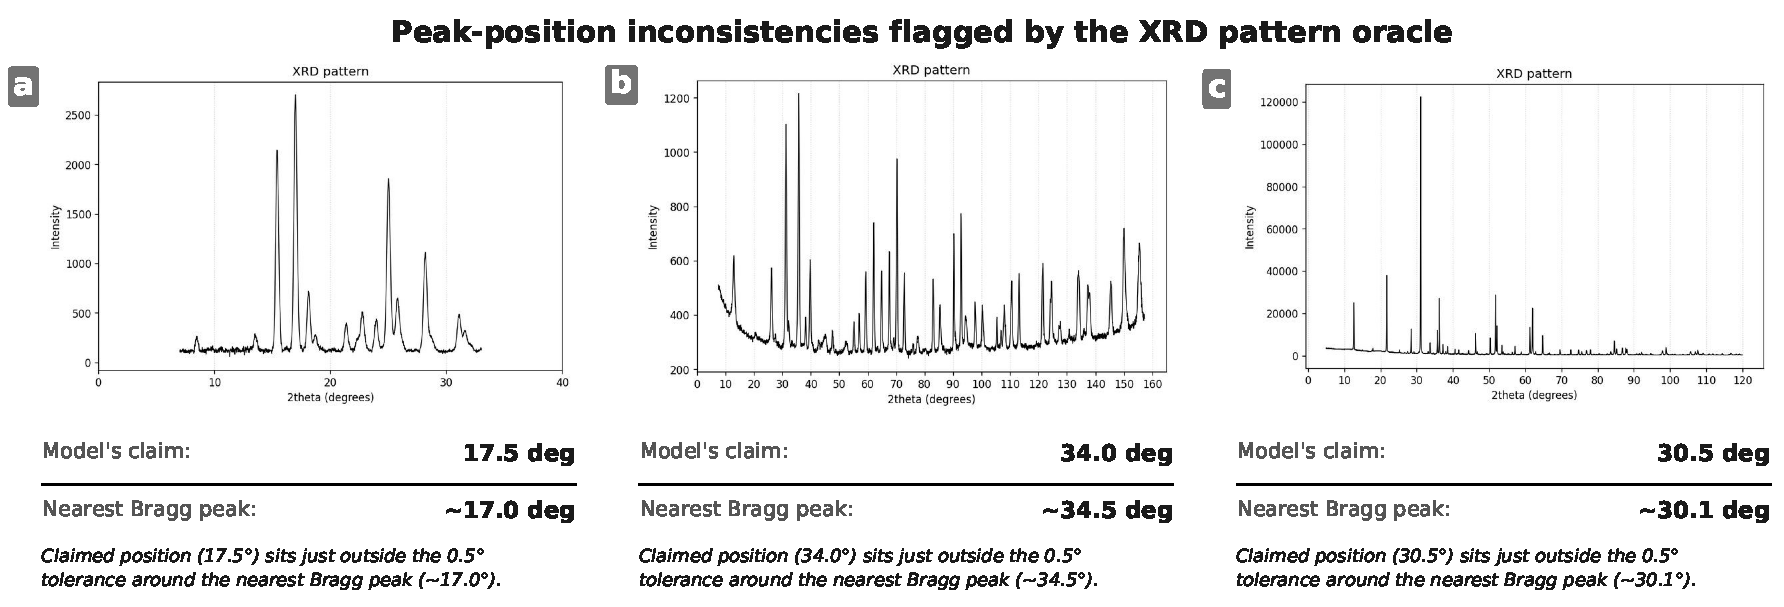
\includegraphics[width=\linewidth]{new_xrd_oracle_figure.pdf}
%\caption{\textbf{Peak-position inconsistencies flagged by the diffraction oracle.} Three
%real, human-confirmed oracle-fired cases: the model's claimed $2\theta$ position, the
%nearest genuine Bragg reflection in the same real diffractogram, and the resulting
%tolerance violation. All three claims sit just outside the oracle's $0.5^\circ$ tolerance
%window around a real peak, consistent with the tolerance-driven false-positive pattern
%described above.}
%\label{fig:xrd-oracle-examples}
%\end{figure}

%\begin{figure}[t]
%\centering
%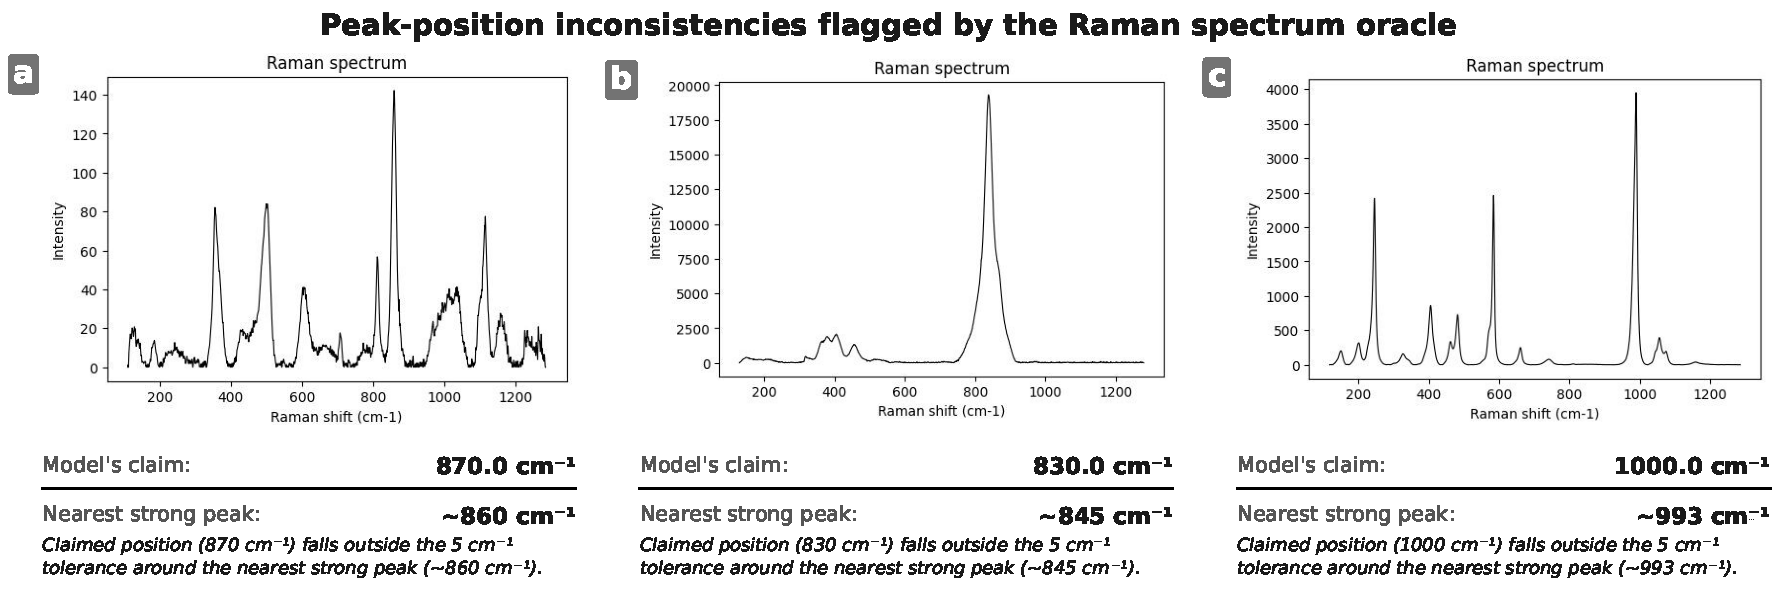
\includegraphics[width=\linewidth]{new_raman_oracle_figure.pdf}
%\caption{\textbf{Peak-position inconsistencies flagged by the Raman spectrum oracle.}
%Three real, human-confirmed oracle-fired cases: the model's claimed Raman shift, the
%nearest genuine strong peak in the same real spectrum, and the resulting tolerance
%violation. All three claims sit just outside the oracle's %$5\,\mathrm{cm}^{-1}$ tolerance
%window around a real peak, the same root cause identified for 34 of 36 %(94\%) of the
%revised spectrum oracle's false positives.}
%\label{fig:raman-oracle-examples}
%\end{figure}

%\begin{figure}[t]
%\centering
%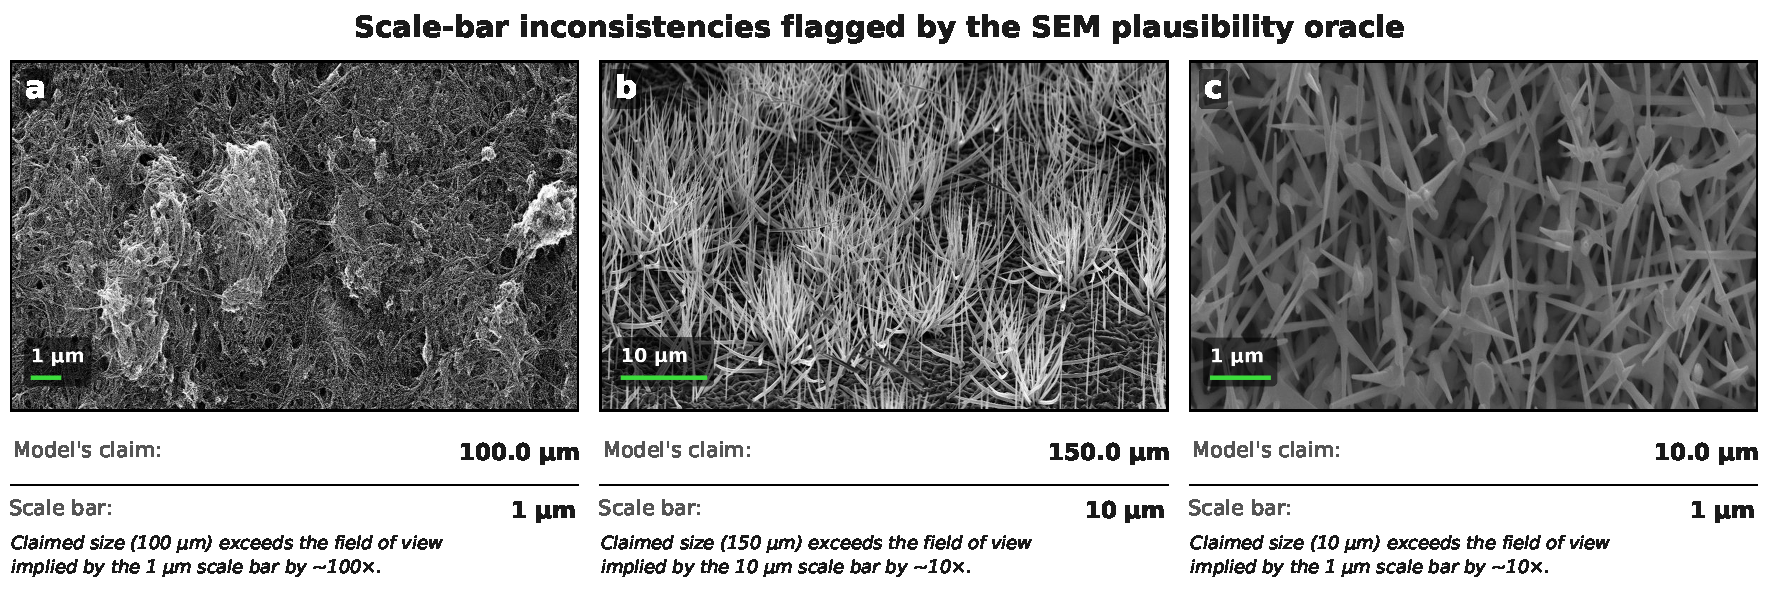
\includegraphics[width=\linewidth]{new_sem_oracle_figure.pdf}
%\caption{\textbf{Scale-bar inconsistencies flagged by the microscopy oracle.} Three real,
%human-confirmed oracle-fired cases: the model's claimed feature size against the real,
%burned-in scale bar of the same NFFA-EUROPE micrograph. Claimed sizes exceed the field of
%view the scale bar implies by roughly $10$--$100\times$, consistent with the scale-bar
%unit and scale-factor arithmetic errors that dominate the microscopy violation taxonomy
%(Results).}
%\label{fig:sem-oracle-examples}
%\end{figure}



\begin{figure}[!htbp]
    \centering

    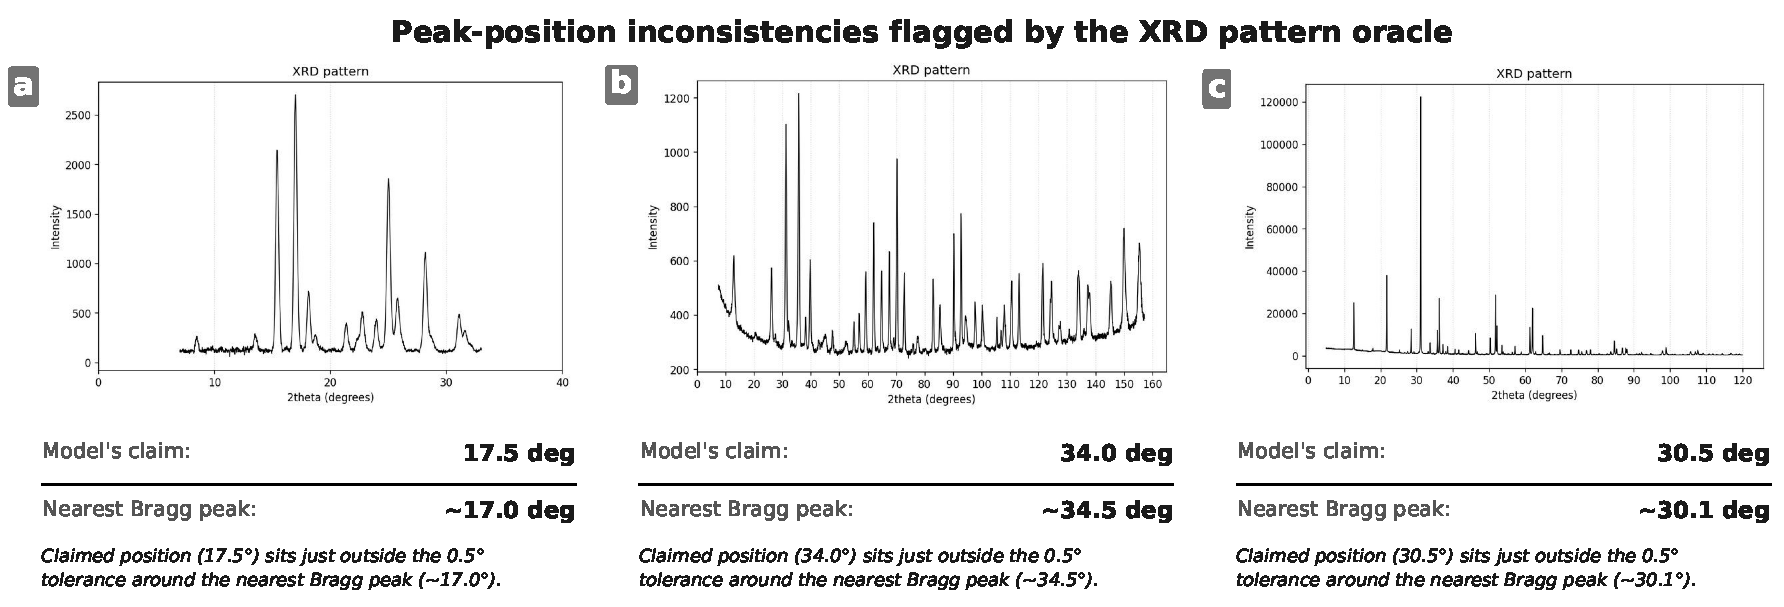
\includegraphics[width=\linewidth,height=0.235\textheight,keepaspectratio]
    {new_xrd_oracle_figure.pdf}

    \vspace{1mm}

    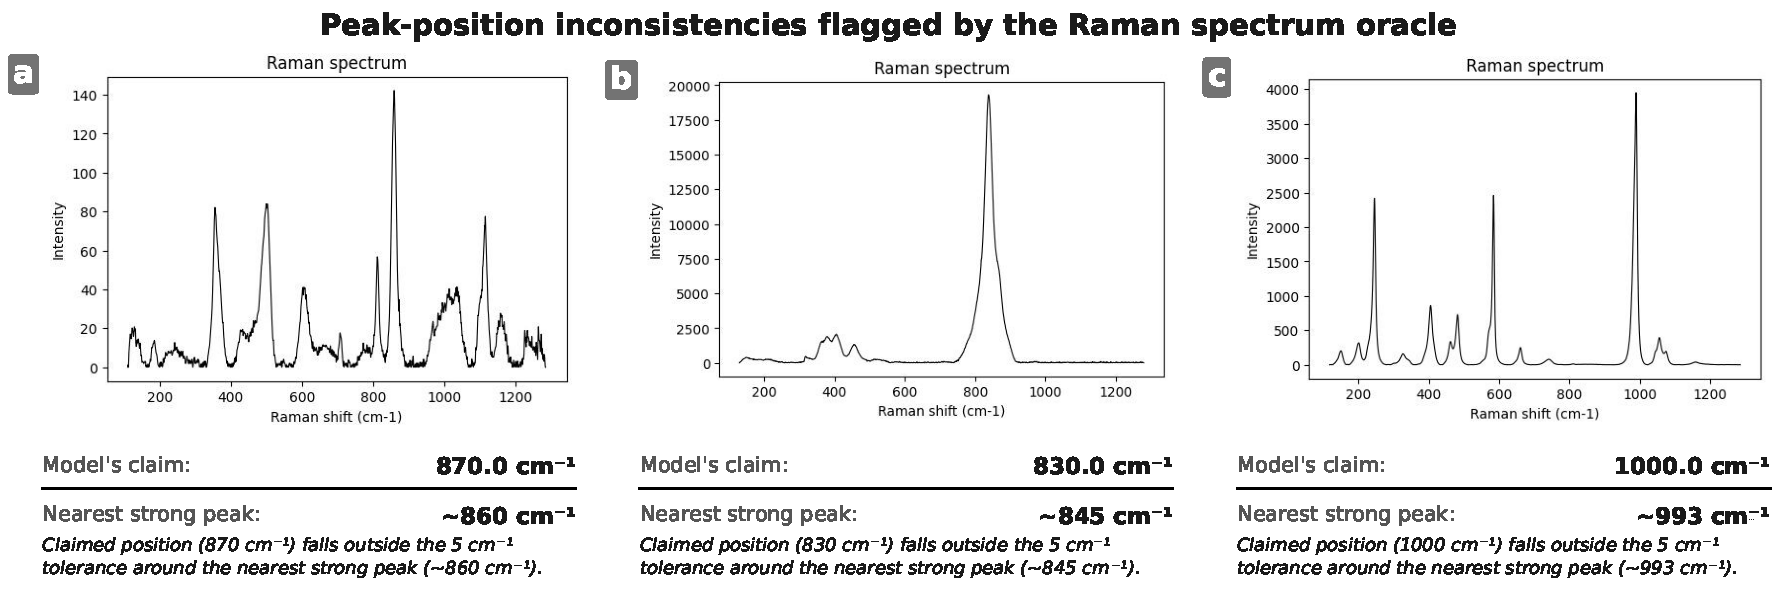
\includegraphics[width=\linewidth,height=0.235\textheight,keepaspectratio]
    {new_raman_oracle_figure.pdf}

    \vspace{1mm}

    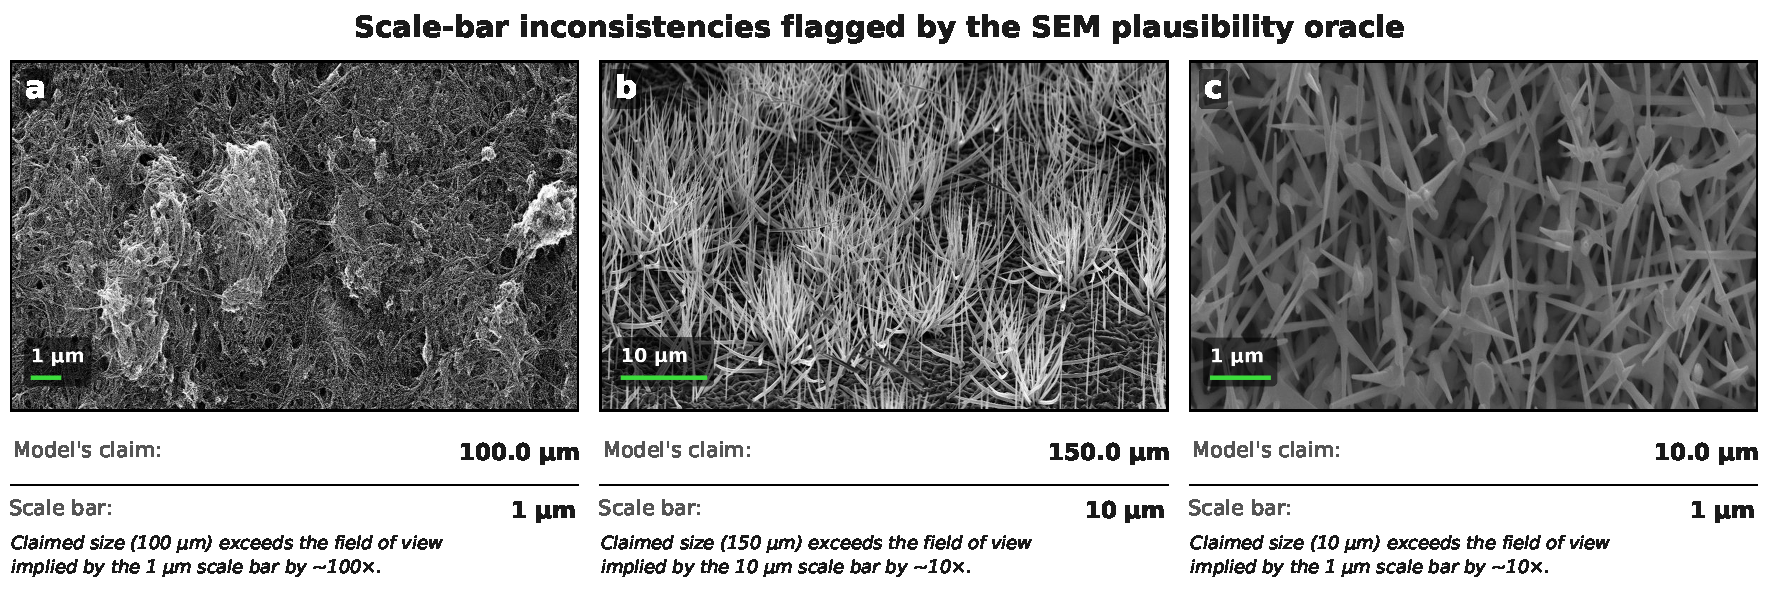
\includegraphics[width=\linewidth,height=0.235\textheight,keepaspectratio]
    {new_sem_oracle_figure.pdf}

    \caption{\justifying\textbf{Representative inconsistencies identified by the multimodal
    oracles.}
    \textbf{a}, X-ray diffraction cases in which the model-reported
    $2\theta$ position lies outside the $0.5^\circ$ tolerance around the nearest
    genuine Bragg reflection.
    \textbf{b}, Raman spectroscopy cases in which the model-reported Raman shift
    exceeds the $5\,\mathrm{cm}^{-1}$ tolerance relative to the nearest genuine
    spectral peak.
    \textbf{c}, Microscopy cases in which the model-reported feature size is
    inconsistent with the physical scale indicated by the embedded scale bar,
    producing discrepancies of approximately $10$--$100\times$.
    All examples are human-confirmed oracle activations and illustrate
    representative tolerance, unit-conversion, and scale-factor failure modes.}

    \label{fig:oracle-examples}
\end{figure}



\begin{table}[t]
\centering
\caption{\justifying\textbf{Oracle validity and audited precision.} The positive-control
false-negative rate is the maximum across three planted violation rates (10\%, 30\%, and 50\%);
all three rates yielded 0.0000 for every oracle family\rev{, which measures completeness on the
injected violation types only}. Audited precision is the fraction of oracle-fired cases from
Qwen2.5-VL-7B and Gemini 2.5 Flash Lite outputs that human review confirmed as genuine
violations of the stated constraint rather than parsing or oracle artifacts\rev{, with Wilson
95\% intervals; $n$ counts decided cases (2 spectrum cases marked unsure are excluded; counting
them either way gives 92.3--92.7\%). Every audit was sampled and judged under the final oracle
definitions used for all reported results (Methods): spectrum responses were collected once and the fired
set re-scored with the final oracle before the audit, and DFT responses were re-collected under the final
definitions before the audit; the diffraction and microscopy audits were carried out in July 2026 and the others in August 2026. Sources: NFFA, NFFA-EUROPE; MP, Materials Project.
$^{a}$Final stability oracle with the near-hull abstention band: the 50 audited cases with
$0<E_{\mathrm{hull}}\le0.05$ eV\,atom$^{-1}$ are not scored; under the original rule the audit gave 95.3\%
[89.5, 98.0] ($n=107$). Consensus: a second annotator, blind to the first labels, re-labelled a random
subsample of 30 audited cases per family stratified by the first annotator's verdict, and the two annotators
adjudicated together every case on which they disagreed (24 in total); the consensus precision is weighted back
to the audited population by stratum, with 95\% intervals from per-stratum Jeffreys posteriors (30 subsampled
cases per family; $^{b}$14, the subsampled stability cases scored under the final oracle). Agreement statistics and the oracle-silent audit are in Supplementary Table~S8.
The full audits were performed by one annotator (R.K.).}}
\label{tab:exp1}
{\scriptsize\setlength{\tabcolsep}{2.5pt}\renewcommand{\arraystretch}{1.12}
\begin{tabular}{l l S[table-format=1.4] c c}
\toprule
Oracle family & Source & {FN rate} & \multicolumn{2}{c}{Audited precision, \% [95\% CI]} \\
\cmidrule(lr){3-3}\cmidrule(lr){4-5}
& & {\itshape positive control} & {\itshape one annotator ($n$)} & \rev{\itshape two-annotator consensus} \\
\midrule
\multicolumn{5}{l}{\itshape Geometric oracles}\\
Diffraction & opXRD & 0.0000 & 77.2 \rev{[68.1, 84.3]} (101) & \rev{60.2 [44.1, 75.4]} \\
Microscopy & NFFA       & 0.0000 & 88.6 \rev{[81.1, 93.3]} (105) & \rev{88.6 [81.8, 93.9]} \\
Raman spectra & RRUFF & 0.0000 & 92.7 \rev{[90.1, 94.7]} (493) & \rev{60.8 [43.6, 76.3]} \\
\addlinespace
\multicolumn{5}{l}{\itshape DFT-grounded oracles}\\
Stability & MP & 0.0000 & \rev{100 [93.7, 100] (57)$^{a}$} & \rev{100 [84.3, 100]$^{b}$} \\
Metallicity & MP & 0.0000 & 94.7 \rev{[89.0, 97.6]} (114) & \rev{94.7 [86.8, 97.0]} \\
Magnetism & MP & 0.0000 & 92.2 \rev{[85.8, 95.8]} (115) & \rev{91.4 [79.9, 96.5]} \\
\bottomrule
\end{tabular}}
\end{table}

\subsection*{Physical consistency of current models}
We measure the Physical-Consistency Rate and per-constraint-type violation rates for
the four originally evaluated models, four later-generation frontier or open models, and
one flagship-tier addition
across diffraction, microscopy, spectra, and
DFT-grounded constraints, separately for image (VLM) and structure or text (LLM)
inputs (Table~\ref{tab:main}, Fig.~\ref{fig:results}a)\rev{. Each (model, constraint-type) cell
sends 30 items per seed to the model, with $S=3$ seeds (90 items per cell); 4{,}334 of these
responses are scored across the nine models. For the image constraint types all nine models
receive the same items in each seed, so their comparisons are paired; for the DFT constraint
types each model and seed draws its own block of materials, so those comparisons are unpaired.
Not every attempted item can be scored. On diffraction, 64 of the 90 items per cell have a
reference pattern the oracle can use (the rest lack a usable structure); on metallicity, 1--8
items per cell fall in the oracle's abstention band, and on stability 11--19 items per cell are
near-hull materials, which the final stability oracle does not score (Methods). Within the items the oracle can score, the
share of responses that state a checkable quantity (coverage) is at least 0.93 in every cell
except GPT-4o on spectra (0.49; Supplementary Table~S2).} Overall PCR ranges from \rev{0.556
(Qwen3-VL-8B-Instruct) to 0.778 (GPT-5.6-Sol, with GPT-5.6-Terra at 0.777)}; models are
markedly more consistent on microscopy (0.67--1.00) than on spectra (0.07--0.83) or
diffraction (0.47--0.82), and the DFT-grounded column is more tightly clustered
(\rev{0.65--0.76}) than any single geometric constraint\rev{.}

\rev{Because PCR excludes responses that state no checkable quantity, a model could in
principle raise its score by stating less. We therefore also scored every cell under two
alternative conventions: counting a non-checkable response as a violation (penalised) and as
consistent (lenient). The overall ordering of the nine models is nearly unchanged (Kendall
$\tau=0.83$ between the reported and penalised conventions and $1.00$ between the reported and
lenient ones); the main change is GPT-4o, from third to fifth under the penalised
convention, because of its low coverage on spectra (Supplementary Table~S2).}

\rev{We test model differences at the item level rather than by comparing interval overlap:
exact McNemar tests on the paired image-arm items, Fisher exact tests on the unpaired DFT items,
and, for overall PCR, a bootstrap that resamples paired items jointly and DFT items within
model (Methods). Holm correction is applied within each family of comparisons (Supplementary
Table~S3). GPT-5.6-Terra exceeds GPT-4o overall by 0.072 (95\% CI $[0.018,0.125]$, Holm
$p=0.045$). Claude Opus 4.6 versus Claude Sonnet 4.5 ($-0.003$, $[-0.050,0.044]$),
Qwen3-VL-8B-Thinking versus Qwen3-VL-8B-Instruct ($+0.034$, $[-0.016,0.083]$) and
GPT-5.6-Sol versus GPT-5.6-Terra ($+0.002$, $[-0.042,0.046]$) are not significant. With
roughly 500 checkable items per model, the smallest overall difference the design detects with
80\% power is 0.064--0.079 depending on the pair, so these three comparisons exclude only
differences larger than about 0.07; they do not show that the models are equivalent. Across all
36 model pairs, 18 differences in overall PCR survive Holm correction; within single
constraint types the detectable difference is 0.11--0.20, so most per-type rankings are not
resolved. On microscopy, the locally run Qwen2.5-VL-7B is the weakest model (0.667, 95\% CI
$[0.563,0.759]$), and seven of the other eight models exceed it after Holm correction (paired
differences $+0.22$ to $+0.33$), while Qwen3-VL-8B-Instruct ($+0.14$, Holm $p=0.12$) does not.} We do not
know whether the gap reflects genuine scale-bar-reading skill or a difference in how each model handles the
info-bar layout variety in the source micrographs, and do not claim more than the
measured difference. The high absolute microscopy rates should also be read against the
looseness of this oracle, which flags only feature sizes exceeding the field of view (a
necessary, not sufficient, condition), so a near-ceiling rate partly reflects an easily
satisfied check. \rev{Diffraction comparisons in particular should be treated as provisional:
the diffraction ranking changes both when the oracle tolerance is varied and when the prompt is
paraphrased (Methods).}

\rev{The DFT column is also sensitive to class composition. The sampled materials are
imbalanced (for stability, only 3--9 of the 70--79 scored materials per model lie on the hull), so a
model that defaults to the majority answer scores well on pooled PCR. Qwen2.5-VL-7B reaches a pooled
stability PCR of 0.917 but answers none of its 4 on-hull materials consistently, a class-balanced rate
of 0.485, whereas GPT-5.6-Terra has the lowest pooled stability PCR (0.653) but a class-balanced rate of
0.814 (Supplementary Table~S4); with so few on-hull materials per model, these class-balanced rates are
imprecise. The ordering of models on the DFT constraint types therefore depends on whether PCR is pooled
or class-balanced, and we report both. To make the DFT comparisons paired as well, we evaluated the
models on one common item set of 90 materials per DFT constraint type, drawn 45 from each reference
class (Supplementary Table~S6); for stability, 34 of the 45 near-hull draws fall in the band the final
oracle does not score, leaving 56 scored materials (11 on the hull, 45 above it). Eight models are
included; Qwen3-VL-8B-Thinking could not be run because its provider endpoint had been withdrawn by the
time of this analysis, and the locally run Qwen2.5-VL-7B was run on CPU in single precision, because no
GPU with bfloat16 support was available then. On this paired set, restricted to the DFT constraint
types, none of the comparisons stated above is significant: GPT-5.6-Terra versus GPT-4o $+0.021$ (95\% CI
$[-0.042,0.085]$), Claude Opus 4.6 versus Claude Sonnet 4.5 $+0.021$ ($[-0.030,0.072]$) and GPT-5.6-Sol
versus GPT-5.6-Terra $+0.030$ ($[-0.013,0.072]$); 3 of the 28 model pairs differ after Holm correction,
all of them Gemini 2.5 Flash Lite scoring lower. The difference between GPT-5.6-Terra and GPT-4o in the
main evaluation therefore comes from the image constraint types, chiefly spectra. The balanced set also
shows a shared failure that the imbalanced sample hid: every model is far less consistent on
computed-metallic compositions (PCR 0.21--0.40) than on gapped ones (0.84--0.96), that is, models
default to calling a composition non-metallic.}

\begin{table}[t]
\centering
\caption{\justifying Main evaluation: Physical-Consistency Rate by constraint type and overall,
\rev{over the checkable responses among 30 attempted items} per (model, constraint-type) cell per seed, $S=3$ seeds pooled per cell
(bootstrap 95\% CIs omitted from this compact view; see Supplementary Table~S1 for the
full per-cell confidence intervals \rev{and checkable counts, Supplementary Table~S2 for coverage
and alternative conventions, Supplementary Table~S3 for paired, Holm-corrected model comparisons,
and Supplementary Table~S4 for class-balanced DFT rates}, and the Methods for why $\rho_t=1-\mathrm{PCR}$ here). DFT column combines the stability, metallicity,
and magnitude constraint types\rev{; near-hull stability materials are not scored (Methods; the original
rule's values are in Supplementary Table~S7)}.  The first four rows are the
originally evaluated models; the next four are the later-generation refresh
(Methods, Baselines subsection). $^{\ddagger}$GPT-5.6-Sol is OpenAI's flagship tier, added
to test whether it exceeds the balanced-tier GPT-5.6-Terra within the same
generation; \rev{the overall difference is $+0.002$ (95\% CI $[-0.042,0.046]$), not significant, so
the design detects no difference between flagship and balanced tier larger than about 0.07}
(Discussion). \rev{Bold marks the column maximum; it does not imply a significant difference from
the next model.}}
\label{tab:main}
{\scriptsize\setlength{\tabcolsep}{5pt}\renewcommand{\arraystretch}{1.12}
\begin{tabular}{l *{5}{S[table-format=1.3]}}
\toprule
& \multicolumn{5}{c}{Physical-Consistency Rate (higher is more consistent)} \\
\cmidrule(lr){2-6}
Model & {Diffraction} & {Microscopy} & {Spectra} & {DFT$^{*}$} & {All$^{*}$} \\
\midrule
Qwen2.5-VL-7B \textit{(open)} & 0.500 & 0.667 & 0.148 & \rev{0.731} & \rev{0.584} \\
Gemini 2.5 Flash Lite & 0.517 & \bfseries 1.000 & 0.278 & \rev{0.658} & \rev{0.630} \\
GPT-4o                & 0.625 & 0.954 & 0.068 & \rev{0.740} & \rev{0.699} \\
Claude Sonnet 4.5     & 0.547 & 0.977 & 0.189 & \bfseries \rev{0.762} & \rev{0.667} \\
\addlinespace
Claude Opus 4.6            & 0.578 & 0.954 & 0.244 & \rev{0.734} & \rev{0.663} \\
GPT-5.6-Terra              & 0.797 & 0.951 & \bfseries 0.833 & \rev{0.696} & \rev{0.777} \\
Qwen3-VL-8B-Instruct       & 0.468 & 0.802 & 0.133 & \rev{0.649} & \rev{0.556} \\
Qwen3-VL-8B-Thinking       & 0.578 & 0.885 & 0.092 & \rev{0.671} & \rev{0.594} \\
\addlinespace
GPT-5.6-Sol$^{\ddagger}$   & \bfseries 0.820 & 0.915 & 0.764 & \rev{0.727} & \bfseries \rev{0.778} \\
\bottomrule
\end{tabular}}
\end{table}


\subsection*{Accuracy versus consistency}
On three constraint types with a genuine, non-circular accuracy criterion distinct
from the oracle's own tolerance (diffraction: agreement with the single nearest true
peak to $0.1^{\circ}$, versus the oracle's looser $0.5^{\circ}$ tolerance; spectra:
agreement with the nearest real measured peak to $2\,\mathrm{cm}^{-1}$, versus the
oracle's prominence-based check; stability: agreement with the Materials
Project \texttt{is\_stable} label, evaluated separately from the oracle's
operational $0.05\,\mathrm{eV\,atom^{-1}}$ near-hull threshold), we report
accuracy alongside PCR and the four-cell breakdown on the same
\rev{838 scored items} ($n=30$ per (model, constraint-type) cell, $S=3$ seeds\rev{, the four originally evaluated
models; this sample is drawn separately from the main evaluation}). Microscopy is excluded: its
prompt elicits only a feature-size claim, so no non-circular accuracy ground truth is
available without a different prompt design. \rev{On the eight diffraction and spectra cells,
accuracy and PCR disagree on a mean of 23.6\% of items, and on stability they coincide
(Fig.~\ref{fig:pipeline}b,c). Part of the diffraction and spectra disagreement is definitional rather
than evidence of reasoning errors that accuracy misses: the accuracy criteria are deliberately tighter
than the oracle tolerances, so the two scores are expected to differ on items that fall between the two
thresholds. What the comparison does establish is that
the two scores measure different properties of the same response, not that PCR detects errors that
accuracy cannot.} Diffraction is dominated by items
that are wrong by the tight accuracy criterion yet still oracle-consistent (up to 36
of 62 items in one diffraction cell, gap 58.1\%): models are frequently close enough to satisfy the
oracle's looser tolerance while measurably off the exact peak. \rev{On spectra, most responses
are wrong by both criteria, so the two scores disagree on few items} (4.2--11.2\% across models). \rev{On stability the two scores coincide under the final protocol,
and this is informative in itself. The oracle's $0.05\,\mathrm{eV\,atom^{-1}}$ near-hull threshold and
Materials Project's own \texttt{is\_stable} label (true only on the hull) disagree on 571 of 3,000 real
entries (19.0\%), and every one of those is a near-hull material, $0<E_{\mathrm{hull}}\le0.05$. The final
oracle does not score that band (Methods), so outside it the two definitions agree, and the stability gap
of 18.0--27.8\% reported under the original rule came entirely from the near-hull materials. The stability
arm still shows the base-rate confound: Qwen2.5-VL-7B is accurate on 61 of 62 unstable materials but on
none of the 8 stable ones, so its near-ceiling raw accuracy reflects the base rate rather than
discriminative skill. Balanced accuracy (the mean of per-class accuracy) is 0.492 (Qwen2.5-VL-7B), 0.690
(Gemini 2.5 Flash Lite), 0.492 (GPT-4o) and 0.992 (Claude Sonnet 4.5); two of the four models are at
chance once the imbalance is corrected for ($n=65$--73 scored materials per model, 5--8 of them stable).}

\rev{What PCR adds to answer accuracy is therefore not a finer measure of correctness but a
different, label-free property. First, it needs no answer key: it is defined on microscopy and
on net magnetization, where this benchmark has no non-circular accuracy criterion, and on any new
item for which a reference structure, scale bar or computed value exists. Second, it is a floor
rather than a target: a violation is a statement the measurement or the reference calculation
rules out, so a violation is informative about the reasoning that produced it (Fig.~\ref{fig:teaser}c
shows what these violations consist of), whereas an accuracy miss may only reflect reading
precision. Third, because it is a necessary condition, PCR cannot certify that a response is
right; a high PCR with low accuracy, as on diffraction, identifies responses that are physically
admissible but imprecise. We therefore present PCR as a complement to answer accuracy where labels
exist and as a substitute screening signal where they do not, not as a replacement for either.}

\subsection*{Effect of self-verification}
We measure PCR before and after CGSV on identical items and test the change with the
exact paired McNemar test, reporting fixes, regressions, and residual violations
(Table~\ref{tab:cgsv}, Fig.~\ref{fig:results}b), on diffraction and spectra, the two constraint types where
the oracle's feedback is an actionable physical constraint the model can re-examine
without the feedback message itself revealing the answer (a scale-bar violation
message would state the conversion factor outright, and the three DFT claim types are
single-shot binary judgments with no intermediate quantity to reconsider). $n=30$
items per (model, constraint-type) cell, $S=3$ seeds, $K=2$ maximum revision rounds, 545
checkable records in total. \rev{Because Algorithm~\ref{alg:cgsv} stops at the first round in which no
violation remains, an item that is consistent before revision is never revised. The absence of
regressions in consistency ($b=0$ in every cell) therefore follows from the stopping rule; it
confirms the implementation but is not evidence about the model.} CGSV raises PCR for all four models pooled across both
constraint types (Qwen2.5-VL-7B $0.338\!\to\!0.439$, $p=3.1\times10^{-5}$; Gemini 2.5
Flash Lite $0.521\!\to\!0.632$, $p=2.4\times10^{-4}$; GPT-4o
$0.434\!\to\!0.593$, $p=7.6\times10^{-6}$; Claude Sonnet 4.5 $0.373\!\to\!0.639$,
$p=4.6\times10^{-13}$\rev{; all survive Holm correction}).
Residual violations remain in every cell after $K=2$ rounds (roughly 40--90\% of
items \rev{on spectra}), so CGSV reduces but does not eliminate violations.

\rev{Because CGSV is scored by the same oracles that supply its feedback, a rise in PCR alone cannot
show that revised answers are more correct. Every item exposes exactly one checkable claim in
every round, so a gain cannot come from the model dropping the claim. To see what the revisions
achieve, we scored each item's first-round and final-round claim against the same non-circular
accuracy criteria as the accuracy-versus-consistency analysis ($0.1^\circ$ for diffraction,
$2\,\mathrm{cm}^{-1}$ for spectra) and compared them on the same items (Table~\ref{tab:cgsvacc}).
Accuracy is a property the loop never observes, so unlike consistency it can regress. On spectra
($n=293$) accuracy rises from 5.8\% to 9.9\%: 14 items become accurate and 2 cease to be (exact
McNemar $p=0.004$). Of the 244 spectrum items the oracle flagged and the model revised, 48 cleared
the oracle; 11 of these moved to the accurate value and 37 to a value the oracle admits but that
is not within the accuracy tolerance, and the remaining 196 stayed inconsistent.
On diffraction ($n=245$; 7 items whose reference pattern could not be computed are omitted) accuracy
rises from 22.9\% to 28.6\%: 14 items become accurate and none ceases to be (exact McNemar $p=0.0001$).
Of the 79 diffraction items the oracle flagged and the model revised, 41 cleared the oracle; 14 of these
moved to the accurate value and 27 to an admissible but inexact one, and 38 stayed inconsistent. Revisions that clear
the oracle therefore mostly move a claim into the physically admissible region rather than onto the
exact value, while also producing a small but significant net gain in correctness. The evidence
supports this narrower statement, not a claim that CGSV corrects the underlying physics in general.}

\rev{We separately ask whether the gain is}
attributable to the oracle signal specifically, or to extra inference-time compute alone,
with three controls matched to CGSV's items, models, and decoding
(Baselines subsection): unaided self-refinement (the model is told to double-check its
answer with no oracle feedback) shows no significant change (before $0.349$, after $0.339$, $n=542$, $b=34$, $c=29$, $p=0.615$);
generic equal-compute re-prompting (the model is simply asked to reconsider) likewise shows
no significant change (before $0.358$, after $0.342$, $n=562$, $b=24$, $c=15$, $p=0.20$). \rev{Both
controls revise every item, including those already consistent, so their nonzero regression counts
are not comparable with CGSV's structural $b=0$; the comparison that matters is the net change,
which is significant for CGSV and absent for both controls.} Best-of-3 independent resampling gives a
random-pick PCR of $0.363$ and an oracle-oracle upper bound (best of 3) of $0.419$
($n=614$). Both fall below CGSV's oracle-guided after-PCR for every model, though the
margin over the weakest, Qwen2.5-VL-7B at $0.439$, is only $0.02$, and the resampling run
draws its own item sample, so we do not test the difference. \rev{These controls show that the PCR gain
is not reproduced by generic self-reflection or by extra sampling at equal compute; they do not
by themselves show that the gain reflects better physics, which is what the paired correctness
analysis above addresses.}

\begin{table}[t]
\centering
\caption{\justifying Effect of Constraint-Grounded Self-Verification, pooled across diffraction
and spectra, $n=30$ items per (model, constraint-type) cell, $S=3$ seeds, $K=2$ rounds.
$\Delta$: PCR gain (after minus before); $b$: regressions (before-consistent,
after-inconsistent); $c$: fixes (before-inconsistent, after-consistent); $p$: exact
two-sided McNemar test on $(b,c)$; $p_{\mathrm{Holm}}$: Holm-Bonferroni-adjusted $p$ over
this table's 6-test family (Methods, Statistics paragraph). All four CGSV effects survive
this correction; both controls remain non-significant. \rev{For CGSV, $b=0$ follows from the stopping
rule (an item consistent before revision is never revised); the controls revise every item, so
their $b$ is not comparable. Paired changes in correctness are in Table~\ref{tab:cgsvacc}.}}
\label{tab:cgsv}
{\scriptsize\setlength{\tabcolsep}{3.4pt}\renewcommand{\arraystretch}{1.12}
\begin{tabular}{l S[table-format=1.3] S[table-format=1.3] S[table-format=+1.3] S[table-format=2.0] S[table-format=2.0] c c}
\toprule
& \multicolumn{3}{c}{PCR} & \multicolumn{2}{c}{Discordant} & & \\
\cmidrule(lr){2-4}\cmidrule(lr){5-6}
Model & {before} & {after} & {$\Delta$} & {$b$} & {$c$} & {$p$} & {$p_{\mathrm{Holm}}$} \\
\midrule
Qwen2.5-VL-7B         & 0.338 & 0.439 & 0.101 & 0 & 16 & $3.1\times10^{-5}$ & $1.2\times10^{-4}$ \\
Gemini 2.5 Flash Lite & 0.521 & 0.632 & 0.111 & 0 & 13 & $2.4\times10^{-4}$ & $7.3\times10^{-4}$ \\
GPT-4o                & 0.434 & 0.593 & \bfseries 0.159 & 0 & 18 & $7.6\times10^{-6}$ & $3.8\times10^{-5}$ \\
Claude Sonnet 4.5     & 0.373 & 0.639 & \bfseries 0.266 & 0 & 42 & $4.6\times10^{-13}$ & $2.7\times10^{-12}$ \\
\midrule
\multicolumn{8}{l}{\itshape Mechanism-isolation controls (pooled across models, both constraint types)}\\
Self-refinement (no oracle) & 0.349 & 0.339 & -0.010 & 34 & 29 & 0.615 & 0.615 \\
Generic re-prompting        & 0.358 & 0.342 & -0.016 & 24 & 15 & 0.20 & 0.399 \\
\bottomrule
\end{tabular}}
\end{table}

\begin{table}[t]
\revon\centering
\caption{\justifying Paired change in answer correctness before and after CGSV, on the same items as
Table~\ref{tab:cgsv}. Accuracy uses the non-circular criteria of the accuracy-versus-consistency
analysis (diffraction: within $0.1^\circ$ of the nearest reference reflection; spectra: within
$2\,\mathrm{cm}^{-1}$ of the nearest detected local maximum), applied to each item's first-round
and final-round claim (accuracy before$\to$after). L/G: items that stop (lost) or start (gained) being
accurate; $p$: exact two-sided McNemar test on (L, G). Rev.: items the oracle flagged at round 1 and the
model revised; of these, A cleared the oracle with an accurate value, Ad cleared it with an admissible
value outside the accuracy tolerance, and U were still flagged after $K=2$ rounds.}
\label{tab:cgsvacc}
{\scriptsize\setlength{\tabcolsep}{2.5pt}\renewcommand{\arraystretch}{1.12}
\begin{tabular}{l l r c c r r c}
\toprule
Constraint & Model & $n$ & Accuracy & L/G & $p$ & Rev. & A/Ad/U \\
\midrule
Spectra & Qwen2.5-VL-7B & 89 & 0.067$\to$0.101 & 0/3 & 0.25 & 80 & 3/9/68 \\
 & Gemini 2.5 F.\ Lite & 69 & 0.043$\to$0.072 & 0/2 & 0.50 & 49 & 2/6/41 \\
 & GPT-4o & 45 & 0.044$\to$0.044 & 1/1 & 1.00 & 40 & 0/4/36 \\
 & Claude Sonnet 4.5 & 90 & 0.067$\to$0.144 & 1/8 & 0.039 & 75 & 6/18/51 \\
 & \textit{pooled} & 293 & 0.058$\to$0.099 & 2/14 & 0.004 & 244 & 11/37/196 \\
\addlinespace
Diffraction & Qwen2.5-VL-7B & 66 & 0.303$\to$0.318 & 0/1 & 1.00 & 24 & 1/3/20 \\
 & Gemini 2.5 F.\ Lite & 47 & 0.213$\to$0.255 & 0/2 & 0.50 & 7 & 2/3/2 \\
 & GPT-4o & 66 & 0.152$\to$0.212 & 0/4 & 0.12 & 24 & 4/10/10 \\
 & Claude Sonnet 4.5 & 66 & 0.242$\to$0.348 & 0/7 & 0.016 & 24 & 7/11/6 \\
 & \textit{pooled} & 245 & 0.229$\to$0.286 & 0/14 & 0.0001 & 79 & 14/27/38 \\
\bottomrule
\end{tabular}}
\end{table}

\subsection*{Verifier for violation prediction}
We fine-tune Qwen2.5-0.5B-Instruct with LoRA on oracle-derived labels alone (no human
annotation) to predict, from the input description and chain text alone, whether a
physical violation is present, using 2{,}152 real oracle-checked records spanning all
six constraint types collected across the preceding evaluations. We report precision,
recall, $F_1$, ROC AUC, and expected calibration error (ECE) on an 80/20
in-distribution split and separately on six held-out-constraint-type splits (train on the
other five constraint types, test on one entirely unseen one). The in-distribution split
is disjoint at the parent source (item or structure) level, \rev{so no source item contributes
records to both sides}. In distribution the verifier is a useful
detector overall (precision 0.77, recall 0.71, $F_1=0.74$, AUC $=0.850$, ECE $=0.096$).
\rev{This pooled figure overstates its usefulness for a given scientific task, for two reasons.
First, the six families have very different violation base rates (19\% for microscopy to 88\%
for spectra in the test split), so a score that only identified the family would already rank
violations above chance: a baseline that assigns each item its family's training-set violation
rate reaches AUC $=0.759$. Second, within single families the verifier's discrimination varies
widely (Table~\ref{tab:verifierfam}): it is strong on microscopy (AUC $0.922$, 95\% CI
$[0.852,0.977]$) and stability ($0.804$, $[0.683,0.903]$), moderate on magnetism ($0.728$,
$[0.562,0.877]$) and diffraction ($0.696$, $[0.493,0.895]$), and not distinguishable from chance on
metallicity ($0.582$, $[0.390,0.775]$) and spectra ($0.513$, $[0.353,0.702]$). The in-distribution
verifier is therefore a useful triage signal for microscopy and stability claims, a weak one for
magnetism and diffraction, and not useful for metallicity or spectra.} Its
cross-constraint-type generalization is poor for all six constraint types: diffraction, microscopy, and stability
are indistinguishable from chance when held out entirely (AUC 0.50, 0.53, and 0.44,
bootstrap 95\% confidence intervals straddling 0.5), spectra is not separable from chance either (AUC
0.56, CI $[0.488,0.626]$)\rev{, magnetism is at chance (AUC $0.503$, $[0.430,0.576]$),} and metallicity is the single arguable exception, with a nominal
95\% interval that excludes chance (AUC 0.58, CI $[0.510,0.652]$) but that no longer does so
once the interval is widened for the six held-out comparisons (Bonferroni-corrected interval
$[0.487,0.673]$). We therefore treat metallicity as a nominal, uncorrected exception rather
than as evidence of transfer, and do not build any claim on it. \rev{No held-out constraint type shows transfer that survives correction for the six comparisons.} We report the verifier as an
in-distribution tool \rev{for the families where it discriminates}, and explicitly do \emph{not} claim it as a general-purpose,
constraint-agnostic violation detector. A pooled AUC across all six held-out constraint
types is not reported: the six held-out runs are separately fine-tuned models, so their raw
probability outputs are not on a directly comparable scale; we report only the six
per-constraint-type numbers (Table~\ref{tab:verifier}, Fig.~\ref{fig:results}c). \rev{The held-out results are sensitive to the training run. The released adapters, retrained
with the same data, splits and seed but in a different numerical precision (Supplementary Note~2),
reproduce the in-distribution AUC exactly ($0.850$) but move the held-out AUCs by up to $0.08$: held-out
microscopy rises to $0.602$, whose interval excludes chance even after Bonferroni correction
($[0.519,0.682]$), and held-out stability falls to $0.383$, below chance. No held-out family reaches a
level useful for triage in either run, which is the conclusion we draw. The verifier was trained on
oracle labels produced under the original stability rule; evaluated only on the test items that the final
oracle scores, its in-distribution AUC is $0.871$ ($[0.834,0.904]$; stability family $0.911$) and its
held-out stability AUC $0.372$, so the conclusions above do not depend on the near-hull band
(Supplementary Note~2).}

\begin{table}[t]
\centering
\caption{\justifying Verifier precision/recall/$F_1$ (in-distribution and held-out-constraint-type
splits, both source-disjoint) and the detector's bootstrap 95\% CI on ROC AUC, predicting a
real oracle violation from held-out verifier scores. Expected calibration error is
reported in the text for the in-distribution split (ECE $=0.096$). No pooled
across-constraint-type AUC is reported (see text).}
\label{tab:verifier}
{\scriptsize\setlength{\tabcolsep}{5pt}\renewcommand{\arraystretch}{1.12}
\begin{tabular}{l S[table-format=1.3] S[table-format=1.3] S[table-format=1.3] S[table-format=1.3] c}
\toprule
& \multicolumn{3}{c}{Violation prediction} & \multicolumn{2}{c}{Detector (ROC)} \\
\cmidrule(lr){2-4}\cmidrule(lr){5-6}
Split & {Precision} & {Recall} & {$F_1$} & {AUC} & {95\% CI} \\
\midrule
\multicolumn{6}{l}{\itshape In distribution (80/20 split, source-disjoint)}\\
All constraint types & 0.768 & 0.706 & 0.735 & \bfseries 0.850 & {[}0.813, 0.883{]} \\
\addlinespace
\multicolumn{6}{l}{\itshape Held out entirely (train on the other five constraint types)}\\
Diffraction (XRD)      & 0.600 & 0.030 & 0.057 & 0.497 & {[}0.419, 0.578{]} \\
Microscopy (SEM)       & 0.239 & 0.905 & 0.378 & 0.527 & {[}0.468, 0.589{]} \\
Spectra (Raman)        & {--} & 0.000 & {--} & 0.558 & {[}0.488, 0.626{]} \\
Stability$^{*}$        & 0.355 & 0.103 & 0.159 & 0.436 & {[}0.370, 0.502{]} \\
Metallicity$^{*}$      & 0.486 & 0.158 & 0.238 & 0.582 & {[}0.510, 0.652{]} \\
Magnetism$^{*}$        & 0.468 & 0.635 & 0.539 & 0.503 & {[}0.430, 0.576{]} \\
\bottomrule
\end{tabular}}
\end{table}

\begin{table}[t]
\revon\centering
\caption{\justifying In-distribution verifier performance within each constraint family (the
source-disjoint 80/20 test split of Table~\ref{tab:verifier}, broken down by family; scores are those of
the single in-distribution model). AUC 95\% CI: bootstrap over source items ($B=5000$).
Viol.: share of test records that are oracle violations. A baseline that scores each record by
its family's training-set violation rate reaches a pooled AUC of 0.759, against the verifier's
0.850. Labels follow the original stability rule; on the items the final rule scores, the stability AUC is
0.911 (Supplementary Note~2).}
\label{tab:verifierfam}
{\scriptsize\setlength{\tabcolsep}{5pt}\renewcommand{\arraystretch}{1.12}
\begin{tabular}{l r r S[table-format=1.3] S[table-format=1.3] S[table-format=1.3] S[table-format=1.3] c}
\toprule
Family & $n$ & {Viol.} & {Precision} & {Recall} & {$F_1$} & {AUC} & {95\% CI} \\
\midrule
Diffraction (XRD)  & 33  & 70\% & 0.846 & 0.478 & 0.611 & 0.696 & {[}0.493, 0.895{]} \\
Microscopy (SEM)   & 109 & 19\% & 0.750 & 0.714 & 0.732 & 0.922 & {[}0.852, 0.977{]} \\
Spectra (Raman)    & 100 & 88\% & 0.880 & 1.000 & 0.936 & 0.513 & {[}0.353, 0.702{]} \\
Stability$^{*}$    & 87  & 31\% & 0.727 & 0.296 & 0.421 & 0.804 & {[}0.683, 0.903{]} \\
Metallicity$^{*}$  & 55  & 35\% & 0.364 & 0.421 & 0.390 & 0.582 & {[}0.390, 0.775{]} \\
Magnetism$^{*}$    & 47  & 40\% & 0.600 & 0.474 & 0.529 & 0.728 & {[}0.562, 0.877{]} \\
\bottomrule
\end{tabular}}
\end{table}

% Figure: main results (heatmap + slopegraph + forest)
\begin{figure}[p]
\centering
\resizebox{0.975\linewidth}{!}{%
\begin{tikzpicture}[font=\sffamily]
\node[plab,anchor=west] at (-0.10,7.62){a)};
\node[font=\sffamily\small\bfseries,anchor=west] at (0.55,7.62){Physical consistency by model and constraint type};
\draw[black!45,line width=0.5pt](2.57,7.10)--(6.89,7.10);
\draw[black!45,line width=0.5pt](6.92,7.10)--(11.24,7.10);
\node[font=\sffamily\fontsize{6.5}{8}\selectfont,black!60,anchor=south] at (4.73,7.14){geometric oracles};
\node[font=\sffamily\fontsize{6.5}{8}\selectfont,black!60,anchor=south] at (9.08,7.14){DFT-grounded oracles};
\node[font=\sffamily\fontsize{6.8}{8}\selectfont,anchor=south] at (3.28,6.60){Diffraction};
\node[font=\sffamily\fontsize{6}{7}\selectfont,black!55,anchor=south] at (3.28,6.30){(XRD)};
\node[font=\sffamily\fontsize{6.8}{8}\selectfont,anchor=south] at (4.73,6.60){Microscopy};
\node[font=\sffamily\fontsize{6}{7}\selectfont,black!55,anchor=south] at (4.73,6.30){(SEM)};
\node[font=\sffamily\fontsize{6.8}{8}\selectfont,anchor=south] at (6.18,6.60){Spectra};
\node[font=\sffamily\fontsize{6}{7}\selectfont,black!55,anchor=south] at (6.18,6.30){(Raman)};
\node[font=\sffamily\fontsize{6.8}{8}\selectfont,anchor=south] at (7.63,6.60){Stability};
\node[font=\sffamily\fontsize{6}{7}\selectfont,black!55,anchor=south] at (7.63,6.30){$^{*}$};
\node[font=\sffamily\fontsize{6.8}{8}\selectfont,anchor=south] at (9.08,6.60){Metallicity};
\node[font=\sffamily\fontsize{6}{7}\selectfont,black!55,anchor=south] at (9.08,6.30){$^{*}$};
\node[font=\sffamily\fontsize{6.8}{8}\selectfont,anchor=south] at (10.53,6.60){Magnetism};
\node[font=\sffamily\fontsize{6}{7}\selectfont,black!55,anchor=south] at (10.53,6.30){$^{*}$};
\node[font=\sffamily\fontsize{6.8}{8}\selectfont\bfseries,anchor=south] at (12.36,6.60){Overall};
\node[font=\sffamily\fontsize{6}{7}\selectfont,black!55,anchor=south] at (12.36,6.30){(all six)};
\node[font=\sffamily\fontsize{6.8}{8}\selectfont,anchor=east] at (2.45,5.23){GPT-5.6-Terra$^{\dagger}$};
\node[minimum width=1.42cm,minimum height=0.56cm,fill=npblue!71,draw=white,line width=1pt,inner sep=0,font=\sffamily\fontsize{7.2}{8}\selectfont,text=white] at (3.28,5.23){0.797};
\node[minimum width=1.42cm,minimum height=0.56cm,fill=npblue!84,draw=white,line width=1pt,inner sep=0,font=\sffamily\fontsize{7.2}{8}\selectfont,text=white] at (4.73,5.23){0.951};
\node[minimum width=1.42cm,minimum height=0.56cm,fill=npblue!74,draw=white,line width=1pt,inner sep=0,font=\sffamily\fontsize{7.2}{8}\selectfont,text=white] at (6.18,5.23){0.833};
\node[minimum width=1.42cm,minimum height=0.56cm,fill=npblue!60,draw=white,line width=1pt,inner sep=0,font=\sffamily\fontsize{7.2}{8}\selectfont,text=white] at (7.63,5.23){0.653};
\node[minimum width=1.42cm,minimum height=0.56cm,fill=npblue!60,draw=white,line width=1pt,inner sep=0,font=\sffamily\fontsize{7.2}{8}\selectfont,text=white] at (9.08,5.23){0.659};
\node[minimum width=1.42cm,minimum height=0.56cm,fill=npblue!69,draw=white,line width=1pt,inner sep=0,font=\sffamily\fontsize{7.2}{8}\selectfont,text=white] at (10.53,5.23){0.767};
\node[minimum width=1.42cm,minimum height=0.56cm,fill=npblue!70,draw=black!45,line width=0.6pt,inner sep=0,font=\sffamily\fontsize{7.2}{8}\selectfont\bfseries,text=white] at (12.36,5.23){0.777};
\node[font=\sffamily\fontsize{6.8}{8}\selectfont,anchor=east] at (2.45,5.85){GPT-5.6-Sol$^{\ddagger}$};
\node[minimum width=1.42cm,minimum height=0.56cm,fill=npblue!73,draw=white,line width=1pt,inner sep=0,font=\sffamily\fontsize{7.2}{8}\selectfont,text=white] at (3.28,5.85){0.820};
\node[minimum width=1.42cm,minimum height=0.56cm,fill=npblue!81,draw=white,line width=1pt,inner sep=0,font=\sffamily\fontsize{7.2}{8}\selectfont,text=white] at (4.73,5.85){0.915};
\node[minimum width=1.42cm,minimum height=0.56cm,fill=npblue!69,draw=white,line width=1pt,inner sep=0,font=\sffamily\fontsize{7.2}{8}\selectfont,text=white] at (6.18,5.85){0.764};
\node[minimum width=1.42cm,minimum height=0.56cm,fill=npblue!71,draw=white,line width=1pt,inner sep=0,font=\sffamily\fontsize{7.2}{8}\selectfont,text=white] at (7.63,5.85){0.789};
\node[minimum width=1.42cm,minimum height=0.56cm,fill=npblue!61,draw=white,line width=1pt,inner sep=0,font=\sffamily\fontsize{7.2}{8}\selectfont,text=white] at (9.08,5.85){0.670};
\node[minimum width=1.42cm,minimum height=0.56cm,fill=npblue!66,draw=white,line width=1pt,inner sep=0,font=\sffamily\fontsize{7.2}{8}\selectfont,text=white] at (10.53,5.85){0.733};
\node[minimum width=1.42cm,minimum height=0.56cm,fill=npblue!70,draw=black!45,line width=0.6pt,inner sep=0,font=\sffamily\fontsize{7.2}{8}\selectfont\bfseries,text=white] at (12.36,5.85){0.778};
\node[font=\sffamily\fontsize{6.8}{8}\selectfont,anchor=east] at (2.45,4.62){GPT-4o};
\node[minimum width=1.42cm,minimum height=0.56cm,fill=npblue!57,draw=white,line width=1pt,inner sep=0,font=\sffamily\fontsize{7.2}{8}\selectfont,text=black] at (3.28,4.62){0.625};
\node[minimum width=1.42cm,minimum height=0.56cm,fill=npblue!84,draw=white,line width=1pt,inner sep=0,font=\sffamily\fontsize{7.2}{8}\selectfont,text=white] at (4.73,4.62){0.954};
\node[minimum width=1.42cm,minimum height=0.56cm,fill=npblue!12,draw=white,line width=1pt,inner sep=0,font=\sffamily\fontsize{7.2}{8}\selectfont,text=black] at (6.18,4.62){0.068};
\node[minimum width=1.42cm,minimum height=0.56cm,fill=npblue!79,draw=white,line width=1pt,inner sep=0,font=\sffamily\fontsize{7.2}{8}\selectfont,text=white] at (7.63,4.62){0.886};
\node[minimum width=1.42cm,minimum height=0.56cm,fill=npblue!61,draw=white,line width=1pt,inner sep=0,font=\sffamily\fontsize{7.2}{8}\selectfont,text=white] at (9.08,4.62){0.671};
\node[minimum width=1.42cm,minimum height=0.56cm,fill=npblue!62,draw=white,line width=1pt,inner sep=0,font=\sffamily\fontsize{7.2}{8}\selectfont,text=white] at (10.53,4.62){0.678};
\node[minimum width=1.42cm,minimum height=0.56cm,fill=npblue!63,draw=black!45,line width=0.6pt,inner sep=0,font=\sffamily\fontsize{7.2}{8}\selectfont\bfseries,text=white] at (12.36,4.62){0.699};
\node[font=\sffamily\fontsize{6.8}{8}\selectfont,anchor=east] at (2.45,4.00){Claude Sonnet 4.5};
\node[minimum width=1.42cm,minimum height=0.56cm,fill=npblue!51,draw=white,line width=1pt,inner sep=0,font=\sffamily\fontsize{7.2}{8}\selectfont,text=black] at (3.28,4.00){0.547};
\node[minimum width=1.42cm,minimum height=0.56cm,fill=npblue!86,draw=white,line width=1pt,inner sep=0,font=\sffamily\fontsize{7.2}{8}\selectfont,text=white] at (4.73,4.00){0.977};
\node[minimum width=1.42cm,minimum height=0.56cm,fill=npblue!21,draw=white,line width=1pt,inner sep=0,font=\sffamily\fontsize{7.2}{8}\selectfont,text=black] at (6.18,4.00){0.189};
\node[minimum width=1.42cm,minimum height=0.56cm,fill=npblue!76,draw=white,line width=1pt,inner sep=0,font=\sffamily\fontsize{7.2}{8}\selectfont,text=white] at (7.63,4.00){0.849};
\node[minimum width=1.42cm,minimum height=0.56cm,fill=npblue!63,draw=white,line width=1pt,inner sep=0,font=\sffamily\fontsize{7.2}{8}\selectfont,text=white] at (9.08,4.00){0.694};
\node[minimum width=1.42cm,minimum height=0.56cm,fill=npblue!68,draw=white,line width=1pt,inner sep=0,font=\sffamily\fontsize{7.2}{8}\selectfont,text=white] at (10.53,4.00){0.756};
\node[minimum width=1.42cm,minimum height=0.56cm,fill=npblue!61,draw=black!45,line width=0.6pt,inner sep=0,font=\sffamily\fontsize{7.2}{8}\selectfont\bfseries,text=white] at (12.36,4.00){0.667};
\node[font=\sffamily\fontsize{6.8}{8}\selectfont,anchor=east] at (2.45,3.39){Claude Opus 4.6$^{\dagger}$};
\node[minimum width=1.42cm,minimum height=0.56cm,fill=npblue!53,draw=white,line width=1pt,inner sep=0,font=\sffamily\fontsize{7.2}{8}\selectfont,text=black] at (3.28,3.39){0.578};
\node[minimum width=1.42cm,minimum height=0.56cm,fill=npblue!84,draw=white,line width=1pt,inner sep=0,font=\sffamily\fontsize{7.2}{8}\selectfont,text=white] at (4.73,3.39){0.954};
\node[minimum width=1.42cm,minimum height=0.56cm,fill=npblue!26,draw=white,line width=1pt,inner sep=0,font=\sffamily\fontsize{7.2}{8}\selectfont,text=black] at (6.18,3.39){0.244};
\node[minimum width=1.42cm,minimum height=0.56cm,fill=npblue!71,draw=white,line width=1pt,inner sep=0,font=\sffamily\fontsize{7.2}{8}\selectfont,text=white] at (7.63,3.39){0.789};
\node[minimum width=1.42cm,minimum height=0.56cm,fill=npblue!65,draw=white,line width=1pt,inner sep=0,font=\sffamily\fontsize{7.2}{8}\selectfont,text=white] at (9.08,3.39){0.721};
\node[minimum width=1.42cm,minimum height=0.56cm,fill=npblue!63,draw=white,line width=1pt,inner sep=0,font=\sffamily\fontsize{7.2}{8}\selectfont,text=white] at (10.53,3.39){0.700};
\node[minimum width=1.42cm,minimum height=0.56cm,fill=npblue!60,draw=black!45,line width=0.6pt,inner sep=0,font=\sffamily\fontsize{7.2}{8}\selectfont\bfseries,text=white] at (12.36,3.39){0.663};
\node[font=\sffamily\fontsize{6.8}{8}\selectfont,anchor=east] at (2.45,2.77){Gemini 2.5 Flash Lite};
\node[minimum width=1.42cm,minimum height=0.56cm,fill=npblue!48,draw=white,line width=1pt,inner sep=0,font=\sffamily\fontsize{7.2}{8}\selectfont,text=black] at (3.28,2.77){0.517};
\node[minimum width=1.42cm,minimum height=0.56cm,fill=npblue!88,draw=white,line width=1pt,inner sep=0,font=\sffamily\fontsize{7.2}{8}\selectfont,text=white] at (4.73,2.77){1.000};
\node[minimum width=1.42cm,minimum height=0.56cm,fill=npblue!29,draw=white,line width=1pt,inner sep=0,font=\sffamily\fontsize{7.2}{8}\selectfont,text=black] at (6.18,2.77){0.278};
\node[minimum width=1.42cm,minimum height=0.56cm,fill=npblue!73,draw=white,line width=1pt,inner sep=0,font=\sffamily\fontsize{7.2}{8}\selectfont,text=white] at (7.63,2.77){0.814};
\node[minimum width=1.42cm,minimum height=0.56cm,fill=npblue!64,draw=white,line width=1pt,inner sep=0,font=\sffamily\fontsize{7.2}{8}\selectfont,text=white] at (9.08,2.77){0.702};
\node[minimum width=1.42cm,minimum height=0.56cm,fill=npblue!47,draw=white,line width=1pt,inner sep=0,font=\sffamily\fontsize{7.2}{8}\selectfont,text=black] at (10.53,2.77){0.494};
\node[minimum width=1.42cm,minimum height=0.56cm,fill=npblue!58,draw=black!45,line width=0.6pt,inner sep=0,font=\sffamily\fontsize{7.2}{8}\selectfont\bfseries,text=black] at (12.36,2.77){0.630};
\node[font=\sffamily\fontsize{6.8}{8}\selectfont,anchor=east] at (2.45,2.16){Qwen3-VL-8B-Thinking$^{\dagger}$};
\node[minimum width=1.42cm,minimum height=0.56cm,fill=npblue!53,draw=white,line width=1pt,inner sep=0,font=\sffamily\fontsize{7.2}{8}\selectfont,text=black] at (3.28,2.16){0.578};
\node[minimum width=1.42cm,minimum height=0.56cm,fill=npblue!79,draw=white,line width=1pt,inner sep=0,font=\sffamily\fontsize{7.2}{8}\selectfont,text=white] at (4.73,2.16){0.885};
\node[minimum width=1.42cm,minimum height=0.56cm,fill=npblue!14,draw=white,line width=1pt,inner sep=0,font=\sffamily\fontsize{7.2}{8}\selectfont,text=black] at (6.18,2.16){0.092};
\node[minimum width=1.42cm,minimum height=0.56cm,fill=npblue!79,draw=white,line width=1pt,inner sep=0,font=\sffamily\fontsize{7.2}{8}\selectfont,text=white] at (7.63,2.16){0.895};
\node[minimum width=1.42cm,minimum height=0.56cm,fill=npblue!59,draw=white,line width=1pt,inner sep=0,font=\sffamily\fontsize{7.2}{8}\selectfont,text=black] at (9.08,2.16){0.644};
\node[minimum width=1.42cm,minimum height=0.56cm,fill=npblue!47,draw=white,line width=1pt,inner sep=0,font=\sffamily\fontsize{7.2}{8}\selectfont,text=black] at (10.53,2.16){0.506};
\node[minimum width=1.42cm,minimum height=0.56cm,fill=npblue!55,draw=black!45,line width=0.6pt,inner sep=0,font=\sffamily\fontsize{7.2}{8}\selectfont\bfseries,text=black] at (12.36,2.16){0.594};
\node[font=\sffamily\fontsize{6.8}{8}\selectfont,anchor=east] at (2.45,1.54){Qwen2.5-VL-7B};
\node[minimum width=1.42cm,minimum height=0.56cm,fill=npblue!47,draw=white,line width=1pt,inner sep=0,font=\sffamily\fontsize{7.2}{8}\selectfont,text=black] at (3.28,1.54){0.500};
\node[minimum width=1.42cm,minimum height=0.56cm,fill=npblue!61,draw=white,line width=1pt,inner sep=0,font=\sffamily\fontsize{7.2}{8}\selectfont,text=white] at (4.73,1.54){0.667};
\node[minimum width=1.42cm,minimum height=0.56cm,fill=npblue!18,draw=white,line width=1pt,inner sep=0,font=\sffamily\fontsize{7.2}{8}\selectfont,text=black] at (6.18,1.54){0.148};
\node[minimum width=1.42cm,minimum height=0.56cm,fill=npblue!81,draw=white,line width=1pt,inner sep=0,font=\sffamily\fontsize{7.2}{8}\selectfont,text=white] at (7.63,1.54){0.917};
\node[minimum width=1.42cm,minimum height=0.56cm,fill=npblue!50,draw=white,line width=1pt,inner sep=0,font=\sffamily\fontsize{7.2}{8}\selectfont,text=black] at (9.08,1.54){0.540};
\node[minimum width=1.42cm,minimum height=0.56cm,fill=npblue!69,draw=white,line width=1pt,inner sep=0,font=\sffamily\fontsize{7.2}{8}\selectfont,text=white] at (10.53,1.54){0.767};
\node[minimum width=1.42cm,minimum height=0.56cm,fill=npblue!54,draw=black!45,line width=0.6pt,inner sep=0,font=\sffamily\fontsize{7.2}{8}\selectfont\bfseries,text=black] at (12.36,1.54){0.584};
\node[font=\sffamily\fontsize{6.8}{8}\selectfont,anchor=east] at (2.45,0.92){Qwen3-VL-8B-Instruct$^{\dagger}$};
\node[minimum width=1.42cm,minimum height=0.56cm,fill=npblue!44,draw=white,line width=1pt,inner sep=0,font=\sffamily\fontsize{7.2}{8}\selectfont,text=black] at (3.28,0.92){0.468};
\node[minimum width=1.42cm,minimum height=0.56cm,fill=npblue!72,draw=white,line width=1pt,inner sep=0,font=\sffamily\fontsize{7.2}{8}\selectfont,text=white] at (4.73,0.92){0.802};
\node[minimum width=1.42cm,minimum height=0.56cm,fill=npblue!17,draw=white,line width=1pt,inner sep=0,font=\sffamily\fontsize{7.2}{8}\selectfont,text=black] at (6.18,0.92){0.133};
\node[minimum width=1.42cm,minimum height=0.56cm,fill=npblue!67,draw=white,line width=1pt,inner sep=0,font=\sffamily\fontsize{7.2}{8}\selectfont,text=white] at (7.63,0.92){0.747};
\node[minimum width=1.42cm,minimum height=0.56cm,fill=npblue!62,draw=white,line width=1pt,inner sep=0,font=\sffamily\fontsize{7.2}{8}\selectfont,text=white] at (9.08,0.92){0.688};
\node[minimum width=1.42cm,minimum height=0.56cm,fill=npblue!50,draw=white,line width=1pt,inner sep=0,font=\sffamily\fontsize{7.2}{8}\selectfont,text=black] at (10.53,0.92){0.533};
\node[minimum width=1.42cm,minimum height=0.56cm,fill=npblue!52,draw=black!45,line width=0.6pt,inner sep=0,font=\sffamily\fontsize{7.2}{8}\selectfont\bfseries,text=black] at (12.36,0.92){0.556};
\foreach \i in {0,...,39}{\pgfmathsetmacro{\ff}{6+\i*2.205}\fill[npblue!\ff] (4.3+\i*0.1,0.00) rectangle (4.3+\i*0.1+0.1,0.00+0.20);}
\draw[black!40,line width=0.4pt](4.3,0.00) rectangle (8.3,0.00+0.20);
\draw[black!40,line width=0.4pt](4.30,0.00)--(4.30,0.00-0.06);
\node[font=\sffamily\fontsize{6}{7}\selectfont,anchor=north] at (4.30,0.00-0.07){0.00};
\draw[black!40,line width=0.4pt](5.30,0.00)--(5.30,0.00-0.06);
\node[font=\sffamily\fontsize{6}{7}\selectfont,anchor=north] at (5.30,0.00-0.07){0.25};
\draw[black!40,line width=0.4pt](6.30,0.00)--(6.30,0.00-0.06);
\node[font=\sffamily\fontsize{6}{7}\selectfont,anchor=north] at (6.30,0.00-0.07){0.50};
\draw[black!40,line width=0.4pt](7.30,0.00)--(7.30,0.00-0.06);
\node[font=\sffamily\fontsize{6}{7}\selectfont,anchor=north] at (7.30,0.00-0.07){0.75};
\draw[black!40,line width=0.4pt](8.30,0.00)--(8.30,0.00-0.06);
\node[font=\sffamily\fontsize{6}{7}\selectfont,anchor=north] at (8.30,0.00-0.07){1.00};
\node[font=\sffamily\fontsize{6.5}{8}\selectfont,anchor=east] at (4.1499999999999995,0.00+0.10){Physical-Consistency Rate};
\node[font=\sffamily\fontsize{6}{7}\selectfont,black!55,anchor=west] at (8.600000000000001,0.00+0.10){$^{\dagger}$later-generation refresh\ \ $^{\ddagger}$flagship addition};
\begin{scope}[shift={(0,-7.17)}]
\node[plab,anchor=west] at (-0.10,5.62){b)};
\node[font=\sffamily\fontsize{7.6}{9}\selectfont\bfseries,anchor=west] at (0.52,5.62){Oracle feedback raises PCR};
\def\yb#1{0.62 + (#1-0.30)/0.40*3.85}
\draw[black!45,line width=0.5pt](1.05,0.62)--(1.05,4.47);
\node[font=\sffamily\fontsize{6.3}{7}\selectfont,anchor=east] at (0.99,{\yb{0.3}}){0.3};
\draw[black!45,line width=0.4pt](1.00,{\yb{0.3}})--(1.18,{\yb{0.3}});
\node[font=\sffamily\fontsize{6.3}{7}\selectfont,anchor=east] at (0.99,{\yb{0.4}}){0.4};
\draw[black!45,line width=0.4pt](1.00,{\yb{0.4}})--(1.18,{\yb{0.4}});
\node[font=\sffamily\fontsize{6.3}{7}\selectfont,anchor=east] at (0.99,{\yb{0.5}}){0.5};
\draw[black!45,line width=0.4pt](1.00,{\yb{0.5}})--(1.18,{\yb{0.5}});
\node[font=\sffamily\fontsize{6.3}{7}\selectfont,anchor=east] at (0.99,{\yb{0.6}}){0.6};
\draw[black!45,line width=0.4pt](1.00,{\yb{0.6}})--(1.18,{\yb{0.6}});
\node[font=\sffamily\fontsize{6.3}{7}\selectfont,anchor=east] at (0.99,{\yb{0.7}}){0.7};
\draw[black!45,line width=0.4pt](1.00,{\yb{0.7}})--(1.18,{\yb{0.7}});
\draw[black!10,line width=0.4pt](1.18,{\yb{0.4}})--(3.70,{\yb{0.4}});
\draw[black!10,line width=0.4pt](1.18,{\yb{0.5}})--(3.70,{\yb{0.5}});
\draw[black!10,line width=0.4pt](1.18,{\yb{0.6}})--(3.70,{\yb{0.6}});
\draw[black!10,line width=0.4pt](1.18,{\yb{0.7}})--(3.70,{\yb{0.7}});
\node[font=\sffamily\fontsize{6.5}{8}\selectfont,rotate=90,anchor=south] at (0.42,2.55){PCR};
\node[font=\sffamily\fontsize{6.8}{8}\selectfont,anchor=north] at (1.45,0.54){before};
\node[font=\sffamily\fontsize{6.8}{8}\selectfont,anchor=north] at (3.05,0.54){after};
\draw[black!45,line width=1.0pt,dash pattern=on 2pt off 1.4pt](1.45,{\yb{0.349}})--(3.05,{\yb{0.339}});
\fill[black!45](1.45,{\yb{0.349}})circle(2.0pt);\fill[black!45](3.05,{\yb{0.339}})circle(2.0pt);
\draw[black!45,line width=1.0pt,dash pattern=on 2pt off 1.4pt](1.45,{\yb{0.358}})--(3.05,{\yb{0.342}});
\fill[black!45](1.45,{\yb{0.358}})circle(2.0pt);\fill[black!45](3.05,{\yb{0.342}})circle(2.0pt);
\draw[npblue,line width=1.5pt](1.45,{\yb{0.338}})--(3.05,{\yb{0.439}});
\fill[npblue](1.45,{\yb{0.338}})circle(2.4pt);\draw[white,line width=0.5pt](1.45,{\yb{0.338}})circle(2.4pt);
\fill[npblue](3.05,{\yb{0.439}})circle(2.4pt);\draw[white,line width=0.5pt](3.05,{\yb{0.439}})circle(2.4pt);
\draw[nporange,line width=1.5pt](1.45,{\yb{0.521}})--(3.05,{\yb{0.632}});
\fill[nporange](1.45,{\yb{0.521}})circle(2.4pt);\draw[white,line width=0.5pt](1.45,{\yb{0.521}})circle(2.4pt);
\fill[nporange](3.05,{\yb{0.632}})circle(2.4pt);\draw[white,line width=0.5pt](3.05,{\yb{0.632}})circle(2.4pt);
\draw[npgreen,line width=1.5pt](1.45,{\yb{0.434}})--(3.05,{\yb{0.593}});
\fill[npgreen](1.45,{\yb{0.434}})circle(2.4pt);\draw[white,line width=0.5pt](1.45,{\yb{0.434}})circle(2.4pt);
\fill[npgreen](3.05,{\yb{0.593}})circle(2.4pt);\draw[white,line width=0.5pt](3.05,{\yb{0.593}})circle(2.4pt);
\draw[nppurple,line width=1.5pt](1.45,{\yb{0.373}})--(3.05,{\yb{0.639}});
\fill[nppurple](1.45,{\yb{0.373}})circle(2.4pt);\draw[white,line width=0.5pt](1.45,{\yb{0.373}})circle(2.4pt);
\fill[nppurple](3.05,{\yb{0.639}})circle(2.4pt);\draw[white,line width=0.5pt](3.05,{\yb{0.639}})circle(2.4pt);
\draw[nppurple!55,line width=0.4pt](3.20,{\yb{0.639}+0.34})--(3.11,{\yb{0.639}});
\node[font=\sffamily\fontsize{6.3}{7}\selectfont,anchor=west,text=nppurple] at (3.24,{\yb{0.639}+0.34}){Claude Sonnet 4.5$^{***}$};
\node[font=\sffamily\fontsize{6.3}{7}\selectfont,anchor=west,text=nporange] at (3.24,{\yb{0.632}-0.06}){Gemini 2.5 FL$^{***}$};
\node[font=\sffamily\fontsize{6.3}{7}\selectfont,anchor=west,text=npgreen] at (3.24,{\yb{0.593}-0.03}){GPT-4o$^{***}$};
\node[font=\sffamily\fontsize{6.3}{7}\selectfont,anchor=west,text=npblue] at (3.24,{\yb{0.439}}){Qwen2.5-VL-7B$^{***}$};
\node[font=\sffamily\fontsize{6.3}{7}\selectfont,anchor=west,text=black!55,align=left] at (3.24,{\yb{0.341}}){self-refinement\\generic re-prompt\\(both n.s.)};
\node[font=\sffamily\fontsize{5.8}{7}\selectfont,anchor=west,text=black!55] at (0.18,0.06){$^{***}$Holm-adjusted $p<10^{-3}$\rev{; CGSV $b=0$ by design (stopping rule)}};
\end{scope}
\begin{scope}[shift={(6.05,-7.17)}]
\node[plab,anchor=west] at (-0.10,5.62){c)};
\node[font=\sffamily\fontsize{7.6}{9}\selectfont\bfseries,anchor=west] at (0.52,5.62){Violation detection versus baselines};
\def\xa#1{2.55 + (#1-0.25)/0.65*4.05}
\draw[npslate!65,dash pattern=on 2pt off 1.6pt,line width=0.6pt]({\xa{0.5}},0.42)--({\xa{0.5}},5.05);
\node[font=\sffamily\fontsize{6.3}{8}\selectfont\itshape,black!65,anchor=west] at (0.02,5.12){In distribution};
\node[font=\sffamily\fontsize{6.5}{8}\selectfont,anchor=east] at (2.42,4.70){MatPCR verifier};
\draw[npgreen,line width=1.1pt]({\xa{0.813}},4.70)--({\xa{0.883}},4.70);
\draw[npgreen,line width=1.0pt]({\xa{0.813}},4.63)--({\xa{0.813}},4.77);
\draw[npgreen,line width=1.0pt]({\xa{0.883}},4.63)--({\xa{0.883}},4.77);
\fill[npgreen]({\xa{0.85}},4.70)circle(2.4pt);\draw[white,line width=0.5pt]({\xa{0.85}},4.70)circle(2.4pt);
\node[font=\sffamily\fontsize{6.2}{7}\selectfont,anchor=west] at (6.72,4.70){0.850};
\node[font=\sffamily\fontsize{6.5}{8}\selectfont,anchor=east] at (2.42,4.34){Zero-shot LLM judge};
\draw[npslate,line width=1.1pt]({\xa{0.4}},4.34)--({\xa{0.493}},4.34);
\draw[npslate,line width=1.0pt]({\xa{0.4}},4.27)--({\xa{0.4}},4.41);
\draw[npslate,line width=1.0pt]({\xa{0.493}},4.27)--({\xa{0.493}},4.41);
\fill[npslate]({\xa{0.447}},4.34)circle(2.4pt);\draw[white,line width=0.5pt]({\xa{0.447}},4.34)circle(2.4pt);
\node[font=\sffamily\fontsize{6.2}{7}\selectfont,anchor=west] at (6.72,4.34){0.447};
\node[font=\sffamily\fontsize{6.5}{8}\selectfont,anchor=east] at (2.42,3.98){Model self-confidence};
\draw[npslate,line width=1.1pt]({\xa{0.264}},3.98)--({\xa{0.365}},3.98);
\draw[npslate,line width=1.0pt]({\xa{0.264}},3.91)--({\xa{0.264}},4.05);
\draw[npslate,line width=1.0pt]({\xa{0.365}},3.91)--({\xa{0.365}},4.05);
\fill[npslate]({\xa{0.315}},3.98)circle(2.4pt);\draw[white,line width=0.5pt]({\xa{0.315}},3.98)circle(2.4pt);
\node[font=\sffamily\fontsize{6.2}{7}\selectfont,anchor=west] at (6.72,3.98){0.315};
\node[font=\sffamily\fontsize{6.3}{8}\selectfont\itshape,black!65,anchor=west] at (0.02,3.62){Held out (unseen constraint type)};
\node[font=\sffamily\fontsize{6.5}{8}\selectfont,anchor=east] at (2.42,3.20){Metallicity$^{*}$};
\draw[nporange,line width=1.1pt]({\xa{0.51}},3.20)--({\xa{0.652}},3.20);
\draw[nporange,line width=1.0pt]({\xa{0.51}},3.13)--({\xa{0.51}},3.27);
\draw[nporange,line width=1.0pt]({\xa{0.652}},3.13)--({\xa{0.652}},3.27);
\fill[nporange]({\xa{0.582}},3.20)circle(2.4pt);\draw[white,line width=0.5pt]({\xa{0.582}},3.20)circle(2.4pt);
\node[font=\sffamily\fontsize{6.2}{7}\selectfont,anchor=west] at (6.72,3.20){0.582};
\node[font=\sffamily\fontsize{6.5}{8}\selectfont,anchor=east] at (2.42,2.84){Spectra (Raman)};
\draw[npslate,line width=1.1pt]({\xa{0.488}},2.84)--({\xa{0.626}},2.84);
\draw[npslate,line width=1.0pt]({\xa{0.488}},2.77)--({\xa{0.488}},2.91);
\draw[npslate,line width=1.0pt]({\xa{0.626}},2.77)--({\xa{0.626}},2.91);
\fill[npslate]({\xa{0.558}},2.84)circle(2.4pt);\draw[white,line width=0.5pt]({\xa{0.558}},2.84)circle(2.4pt);
\node[font=\sffamily\fontsize{6.2}{7}\selectfont,anchor=west] at (6.72,2.84){0.558};
\node[font=\sffamily\fontsize{6.5}{8}\selectfont,anchor=east] at (2.42,2.48){Microscopy (SEM)};
\draw[npslate,line width=1.1pt]({\xa{0.468}},2.48)--({\xa{0.589}},2.48);
\draw[npslate,line width=1.0pt]({\xa{0.468}},2.41)--({\xa{0.468}},2.55);
\draw[npslate,line width=1.0pt]({\xa{0.589}},2.41)--({\xa{0.589}},2.55);
\fill[npslate]({\xa{0.527}},2.48)circle(2.4pt);\draw[white,line width=0.5pt]({\xa{0.527}},2.48)circle(2.4pt);
\node[font=\sffamily\fontsize{6.2}{7}\selectfont,anchor=west] at (6.72,2.48){0.527};
\node[font=\sffamily\fontsize{6.5}{8}\selectfont,anchor=east] at (2.42,2.12){Magnetism$^{*}$};
\draw[npslate,line width=1.1pt]({\xa{0.43}},2.12)--({\xa{0.576}},2.12);
\draw[npslate,line width=1.0pt]({\xa{0.43}},2.05)--({\xa{0.43}},2.19);
\draw[npslate,line width=1.0pt]({\xa{0.576}},2.05)--({\xa{0.576}},2.19);
\fill[npslate]({\xa{0.503}},2.12)circle(2.4pt);\draw[white,line width=0.5pt]({\xa{0.503}},2.12)circle(2.4pt);
\node[font=\sffamily\fontsize{6.2}{7}\selectfont,anchor=west] at (6.72,2.12){0.503};
\node[font=\sffamily\fontsize{6.5}{8}\selectfont,anchor=east] at (2.42,1.76){Diffraction (XRD)};
\draw[npslate,line width=1.1pt]({\xa{0.419}},1.76)--({\xa{0.578}},1.76);
\draw[npslate,line width=1.0pt]({\xa{0.419}},1.69)--({\xa{0.419}},1.83);
\draw[npslate,line width=1.0pt]({\xa{0.578}},1.69)--({\xa{0.578}},1.83);
\fill[npslate]({\xa{0.497}},1.76)circle(2.4pt);\draw[white,line width=0.5pt]({\xa{0.497}},1.76)circle(2.4pt);
\node[font=\sffamily\fontsize{6.2}{7}\selectfont,anchor=west] at (6.72,1.76){0.497};
\node[font=\sffamily\fontsize{6.5}{8}\selectfont,anchor=east] at (2.42,1.40){Stability$^{*}$};
\draw[npslate,line width=1.1pt]({\xa{0.37}},1.40)--({\xa{0.502}},1.40);
\draw[npslate,line width=1.0pt]({\xa{0.37}},1.33)--({\xa{0.37}},1.47);
\draw[npslate,line width=1.0pt]({\xa{0.502}},1.33)--({\xa{0.502}},1.47);
\fill[npslate]({\xa{0.436}},1.40)circle(2.4pt);\draw[white,line width=0.5pt]({\xa{0.436}},1.40)circle(2.4pt);
\node[font=\sffamily\fontsize{6.2}{7}\selectfont,anchor=west] at (6.72,1.40){0.436};
\draw[black!45,line width=0.5pt](2.55,0.42)--(6.60,0.42);
\draw[black!45,line width=0.4pt]({\xa{0.3}},0.42)--({\xa{0.3}},0.35);
\node[font=\sffamily\fontsize{6.2}{7}\selectfont,anchor=north] at ({\xa{0.3}},0.33){0.3};
\draw[black!45,line width=0.4pt]({\xa{0.4}},0.42)--({\xa{0.4}},0.35);
\node[font=\sffamily\fontsize{6.2}{7}\selectfont,anchor=north] at ({\xa{0.4}},0.33){0.4};
\draw[black!45,line width=0.4pt]({\xa{0.5}},0.42)--({\xa{0.5}},0.35);
\node[font=\sffamily\fontsize{6.2}{7}\selectfont,anchor=north] at ({\xa{0.5}},0.33){0.5};
\draw[black!45,line width=0.4pt]({\xa{0.6}},0.42)--({\xa{0.6}},0.35);
\node[font=\sffamily\fontsize{6.2}{7}\selectfont,anchor=north] at ({\xa{0.6}},0.33){0.6};
\draw[black!45,line width=0.4pt]({\xa{0.7}},0.42)--({\xa{0.7}},0.35);
\node[font=\sffamily\fontsize{6.2}{7}\selectfont,anchor=north] at ({\xa{0.7}},0.33){0.7};
\draw[black!45,line width=0.4pt]({\xa{0.8}},0.42)--({\xa{0.8}},0.35);
\node[font=\sffamily\fontsize{6.2}{7}\selectfont,anchor=north] at ({\xa{0.8}},0.33){0.8};
\draw[black!45,line width=0.4pt]({\xa{0.9}},0.42)--({\xa{0.9}},0.35);
\node[font=\sffamily\fontsize{6.2}{7}\selectfont,anchor=north] at ({\xa{0.9}},0.33){0.9};
\node[font=\sffamily\fontsize{6.5}{8}\selectfont,anchor=north] at (4.55,0.06){Detector AUC with bootstrap 95\% CI};
\node[font=\sffamily\fontsize{5.8}{7}\selectfont,anchor=west,text=npgreen!55!black] at (0.30,-0.42){\rule{6pt}{1.5pt}\,CI above chance};
\node[font=\sffamily\fontsize{5.8}{7}\selectfont,anchor=west,text=nporange!80!black] at (2.55,-0.42){\rule{6pt}{1.5pt}\,nominal CI only};
\node[font=\sffamily\fontsize{5.8}{7}\selectfont,anchor=west,text=npslate] at (4.65,-0.42){\rule{6pt}{1.5pt}\,not above chance};
\end{scope}
\end{tikzpicture}}
\caption{\justifying\textbf{Physical consistency, oracle-driven correction, and violation detection.} \textbf{a)} Physical-Consistency Rate (PCR) for nine models across the six label-free constraint types and overall, ordered by overall PCR; shading is linear in PCR. \rev{Stability uses the final oracle, which does not score near-hull materials. Cells hold 44--90 checkable records; intervals and coverage are in Supplementary Tables~S1 and S2.} $^{\dagger}$Later-generation refresh models; $^{\ddagger}$flagship-tier addition. \textbf{b)} PCR before and after Constraint-Grounded Self-Verification on identical items, with the two matched controls, self-refinement and equal-compute re-prompting (grey, dashed) \rev{(Tables~\ref{tab:cgsv} and~\ref{tab:cgsvacc})}. \textbf{c)} Detector AUC with bootstrap 95\% intervals for the released verifier, two baselines and the six held-out constraint types, on source-disjoint splits \rev{(Table~\ref{tab:verifier})}.}
\label{fig:results}
\end{figure}

% =====================================================================
\section*{Discussion}
% =====================================================================
Across nine models spanning two capability generations and six label-free constraint
types, current models are far from
uniformly consistent (overall PCR \rev{0.556--0.778}), ruling out the scenario in which the
benchmark would be uninformative because every model already satisfies the physics we
check; spectra and diffraction, in particular, remain hard and highly model-dependent. \rev{The
design separates differences in overall PCR larger than about 0.07 (the smallest difference
detectable with 80\% power at $\sim$500 checkable items per model), and within a single constraint
type only differences of roughly 0.11--0.20. At that resolution, one generational difference is
clear: GPT-5.6-Terra exceeds GPT-4o by 0.072 (95\% CI $[0.018,0.125]$, Holm-corrected $p=0.045$), a
difference that comes from the image constraint types and does not appear on the paired DFT item set.
Three other contrasts we examined, Claude Opus 4.6 versus Claude Sonnet 4.5, an explicit reasoning
mode (Qwen3-VL-8B-Thinking versus its non-reasoning sibling), and flagship versus balanced tier
within one generation (GPT-5.6-Sol versus GPT-5.6-Terra), show no detectable difference. These are
single pairs of models, and a null result here excludes only differences larger than about 0.07,
so we do not draw conclusions about capability scaling, reasoning modes or pricing tiers in general;
testing them would need more items per model, more model pairs, and current frontier releases (the
refresh models are one to three provider releases behind the newest available on the collection
date). We leave these questions to future work.} The accuracy-versus-consistency gap (a mean \rev{23.6\%
disagreement across the diffraction and spectra cells}) \rev{shows
that PCR and answer accuracy measure different properties of the same response}\rev{, although part of
the gap is definitional because the accuracy criteria are tighter than the oracle tolerances}: models are frequently
consistent while measurably wrong on diffraction\rev{. For stability, the strict and the operational
definitions of "stable" differ only on near-hull materials, where neither answer is unambiguously right;
excluding that band, as the final oracle does, makes the two definitions agree and also removes a conflict
between the original oracle and its own prompt (Methods)}; separately, one model's near-ceiling raw stability
accuracy is a base-rate artifact of the sampled materials, not discriminative skill, once
balanced accuracy is computed. \rev{The same base-rate effect appears in PCR itself: on the DFT
constraint types, the ordering of models differs between pooled and class-balanced PCR, so both
should be reported. CGSV reduces oracle-detected violations for all four models tested, an effect
that unaided self-refinement and equal-compute re-prompting do not reproduce. Its absence of
consistency regressions is a property of the stopping rule rather than a finding. Paired
before--after scoring shows a small but significant net gain in exact correctness, but most
revisions that clear the oracle move the stated value into the admissible region rather than onto
the exact one; CGSV is best understood as a filter that removes physically inadmissible claims, not
as a general corrector of physical reasoning.} The released verifier is a useful in-distribution
detector \rev{for microscopy and stability claims, weak for magnetism and diffraction, and not useful
for metallicity or spectra; part of its pooled in-distribution AUC ($0.850$) reflects differences in
violation base rate between families (a family-only baseline reaches $0.759$).} Its
cross-constraint-type generalization is the paper's clearest
negative result: \rev{in the reported runs} five of the six held-out constraint types are indistinguishable from
chance, and the sixth (metallicity) separates from chance only before correcting for the
six comparisons\rev{; in the released, retrained adapters held-out microscopy is weakly above chance
(AUC $0.602$) and none of the six reaches a useful level}, consistent with our stated position that a verifier trained on one
constraint type's surface patterns should not be assumed to transfer to another
without direct evidence. Comparator baselines sharpen this picture. In distribution
neither is competitive: a zero-shot LLM-as-judge reaches AUC $0.447$ and the model's own
token-level self-confidence $0.315$, the latter significantly below chance, against the
fine-tuned verifier's $0.850$. Held out, all three are weak, but not uniformly: the
LLM-judge reaches AUC $0.735$ (95\% CI $[0.682,0.790]$) on microscopy, above anything the
fine-tuned verifier achieves on any held-out constraint type, which suggests the fine-tuned
verifier's advantage is specific to the distribution it was trained on rather than a general
superiority over prompting. The central limitation is intrinsic to the approach, not
particular to these results: the oracles bound a class of physically checkable
errors, so PCR is a necessary-not-sufficient reliability signal\rev{, its recall on real responses
is not established by the positive control, and in the present benchmark it scores one stated
quantity per chain rather than every inferential step}, and the released
verifier predicts the oracle signal rather than replacing first-principles ground
truth. As a clearly scoped extension, the verifier could pre-filter candidate
structures before DFT in a small screening study; a first best-of-3 resampling check finds
real but modest headroom over a random pick (PCR 0.363 random-pick vs.\ 0.419 oracle-oracle
ceiling), though we did not build the verifier-as-selector comparison this ceiling would
need to be practically useful, and report it only as a bounded, partial result. A further implication,
which we make possible but do not claim to demonstrate here, is that a label-free,
physics-grounded consistency signal can serve as a verifiable reward for training
materials-reasoning models, extending reinforcement learning from verifiable rewards
to a domain where verification has been under-specified.\cite{scirlvr2026} We also ran a
domain-specific structure-aware model (MatterChat) on the DFT arms as a materials-domain
evaluee (Baselines subsection): it reaches PCR 0.783/0.795/0.850 on stability/metallicity/
magnetism on a shuffled sample of 120 real materials. These rates sit at or above the
general-purpose models' rates on the same three constraint types, but the sample is drawn
separately from the main evaluation, so the comparison is indicative rather than paired,
and it rests on one domain model. Finally,
every DFT-grounded number in this paper (the DFT column of Table~\ref{tab:main}, the
stability arm of the accuracy-versus-consistency analysis, and the metallicity and
magnetism arms of the verifier and detector analyses) rests on Materials Project
reference values and oracle tolerances\rev{, and the DFT tasks give the model a chemical formula
rather than a structure, so where polymorphs of a composition differ in the checked property the
reference entry is not identified by the prompt (Methods).}

% =====================================================================
\section*{Methods}
% =====================================================================
\subsection*{Data sources}
MatPCR draws only on public data for reproducibility and license clarity: experimental
powder diffraction patterns with known structures;\cite{opxrd2025} public scanning electron microscopy (SEM) images that include scale bars;\cite{aversa2018nffa} open Raman spectra;\cite{lafuente2015rruff} and public first-principles data (computed energies, convex hulls, band gaps) from established databases.\cite{matproj2013} No number reported in this paper rests on a first-principles calculation run by the authors: every DFT-grounded reference value used is Materials Project's own standardized computational result, retrieved via the \texttt{mp-api} client (Methods, DFT-grounded oracles); an authors'-own-DFT fallback for missing or questionable Materials Project entries was implemented but never invoked over the reported sample. We also surveyed the simulated diffraction dataset SimXRD-4M\cite{simxrd2024} as a candidate diffraction source, but its schema (units of the tabulated lattice-distance field; the meaning of its integer label) could not be resolved against its documentation with confidence, so it was not used in any reported result; all diffraction numbers in this paper are from real experimental
patterns only.

\subsection*{Tasks, modalities, and exposed constraints}
Each item pairs an input with a question whose faithful answer requires at least one
physically checkable quantity (Fig.~\ref{fig:pipeline}a). Inputs span image items (VLM), such as micrographs and diffraction images, and structure or text items (LLM), such as a crystal structure with a property question. We parse the reasoning chain for stated quantities (peak positions, scale, feature sizes, stability claims, property values) and test each against the matching oracle. An item is checkable if its chain exposes at least one such quantity.

\subsection*{Programmatic geometric oracles}
For diffraction we apply Bragg's law, $\lambda = 2 d \sin\theta$, converting any
claimed $2\theta$ to a $d$-spacing, testing claimed peaks against the reference
pattern of the stated structure within tolerance, and rejecting claims outside the
realizable $2\theta$ window. For microscopy we recover nanometres per pixel from the
detected scale bar and reject any feature larger than the field of view. For spectra
we accept a claimed peak only if a genuine interior local maximum (higher than both
adjacent flanks down to their nearest valleys, rejecting a monotonic rise or a shoulder on a nearby peak) exists near it with prominence exceeding a fraction of the signal's dynamic range\rev{ (the development history of this criterion is summarized in Supplementary Note~2)}.

\rev{\emph{Tolerances relative to the measurements.} We compared each tolerance with the sampling
and peak widths of the data it is applied to (all patterns and spectra used in the main evaluation
or the precision audit). The processed RRUFF spectra are sampled every $0.48\,\mathrm{cm}^{-1}$, and
the full width at half maximum of each spectrum's strongest peak has a median of
$16.9\,\mathrm{cm}^{-1}$ (interquartile range 11.6--24.3; $n=383$). The $\pm5\,\mathrm{cm}^{-1}$ spectrum
tolerance is therefore about ten sampling steps but narrower than the half-width of a typical peak,
so a claim that lands on the flank of a real peak rather than its apex can be flagged; this matches
the false positives found in the audit, 34 of 36 of which lie within $10\,\mathrm{cm}^{-1}$ of a real
peak. The $\pm2\,\mathrm{cm}^{-1}$ accuracy criterion is narrower still and targets the apex itself.
The opXRD patterns are sampled every $0.013^\circ$ in $2\theta$ (median), and the full width at half
maximum of each pattern's strongest peak has a median of $0.12^\circ$ (interquartile range 0.06--0.21;
$n=176$). The $0.5^\circ$ diffraction tolerance is therefore about four times a typical peak width,
generous relative to the measurement; it is instead set by what can be read from the rendered plot
shown to the model, whose $x$ axis spans a median $0.14^\circ$ per pixel, so the tolerance corresponds to
about three to four pixels. The $0.1^\circ$ accuracy criterion is close to a typical peak width and to
one pixel of the plot. These comparisons, together with the tolerance-sensitivity analysis (Baselines),
show which conclusions depend on the chosen tolerance: the diffraction model ranking does, the
spectrum ranking does not.}

\subsection*{DFT-grounded property oracles}
First-principles access extends the oracle from geometry to computed physics, still
without human labels. A stability claim is checked against the energy above the
convex hull computed for the stated composition; a metallicity claim against the
computed band gap; and a magnetism claim against the computed total magnetization,
normalized per atom. Reference values are Materials Project's own standardized
computational references (database version 2026.04.13, \rev{retrieved via the
\texttt{mp-api} client as a 3{,}000-material batch on 2026-08-05 for the reported evaluation; the
precision-audit sample was drawn from a retrieval of the same database version on 2026-07-16, and all
210 audited materials appear with the same identifiers in the 2026-08-05 batch}; GGA/GGA+U relaxation under Materials Project's published standard workflow), described throughout as standardized computational references, not experimental ground truth. \rev{The DFT tasks give the model only a
chemical formula (the prompts are released with the code), and each claim is checked against one
Materials Project entry for that formula. Because polymorphs of one composition can differ in hull
energy, band gap and magnetization, the formula does not always determine the reference class: among
the 540 compositions that occur more than once in the 3{,}000-material batch, the polymorphs disagree
on the scored stability class for 0.8\% (4 of 478 with scorable entries; most stability disagreement
between polymorphs falls in the near-hull band, which is not scored), on the computed band-gap class for
15.6\% and on the net-magnetization class for 16.1\%. To bound the effect on the reported rates, we retrieved every Materials Project
entry for each evaluated composition (6{,}370 entries for 1{,}491 compositions, same database version)
and re-scored each claim against the composition's lowest-energy polymorph. The verdict changes for
12.6\% of stability claims (8.5\% because the ground-state entry lies in the near-hull band and the claim
would be excluded, 4.0\% because the verdict flips) and 10.5\% of metallicity claims (including 2.1\% that
fall in the abstention band under the ground-state entry), and scoring a claim as consistent if any
polymorph supports it changes 3.4\% and 12.0\%. Magnetism claims cannot be re-scored this way, because a
magnetic claim can fail on magnitude while its class matches. A structure-resolved prompt, giving the
model the specific structure rather than the formula, would remove this ambiguity and is a natural
extension.} Because DFT-computed references depend on the exchange-correlation functional (semilocal functionals underestimate band gaps), each oracle is designed around that known error rather than
treating the reference as exact. \emph{Stability (\rev{near-hull criterion with an abstention band})}: \rev{a STABLE claim is consistent
for a material on the computed convex hull ($E_{\mathrm{hull}}=0$, to numerical precision) and an UNSTABLE
claim for a material above it by more than $\epsilon=0.05\,\mathrm{eV\,atom^{-1}}$. Materials with
$0<E_{\mathrm{hull}}\le\epsilon$ are near-hull or potentially metastable; for them neither answer is
unambiguously right, so they form an explicit abstention band and are excluded from PCR, as for
metallicity. This band corrects a conflict in the original oracle, exposed by the second annotation
(Results): the stability prompt instructs the model to treat any borderline or metastable case as
UNSTABLE, while the original oracle required STABLE for every $E_{\mathrm{hull}}\le\epsilon$, so a model
that followed the prompt on a near-hull material was counted as a violation (89 such records in the main
evaluation and 50 of the 107 audited cases). The original rule's results are reported in Supplementary
Table~S7.} The threshold is an operational screening criterion rather than a definition of strict
thermodynamic stability. On a random sample of 3,000 Materials Project entries, the threshold and the
Materials Project \texttt{is\_stable} label disagreed for 571 structures (19.0\%), all of them in the
near-hull band (Materials Project labelled them unstable; the reverse did not occur)\rev{, so under the
final rule the two definitions agree on every scored material}. We additionally report sensitivity at
$\epsilon\in\{0,0.025,0.05,0.10\}\,\mathrm{eV\,atom^{-1}}$, varying the width of the abstention band; all
four widths gave 0\% false-negative and false-positive rates in the positive-control audit.
Figure~\ref{fig:dft-oracle-cases}a shows three model claims evaluated against this operational near-hull criterion. 
\emph{Computed band-gap classification}: a Materials Project band gap
$\leq0.05\,\mathrm{eV}$ is assigned to the computed zero/near-zero-gap
class, whereas a gap $\geq0.20\,\mathrm{eV}$ is assigned to the computed
nonzero-gap class. The intervening range
($0.05$--$0.20\,\mathrm{eV}$) is treated as an explicit abstention band
and excluded from PCR rather than forced into either class. These thresholds
were fixed before the reported evaluation runs. Figure~\ref{fig:dft-oracle-cases}b
shows three examples of model classifications that are inconsistent with the
corresponding Materials Project-computed band-gap references.
\emph{Magnetism (net-magnetization check)}: because a global reversal of all
collinear spins changes the sign of the total magnetization without changing the
physical state, the oracle uses the absolute total magnetization normalized per
atom. The Materials Project reference is classified as finite or near-zero net
magnetization using a threshold of
$0.05\,\mu_{\rm B}\,\mathrm{atom}^{-1}$, fixed before the reported runs.
Only within the finite-net-magnetization class is a claimed magnitude checked
against the reference within one order of magnitude
(Fig.~\ref{fig:dft-oracle-cases}c). This oracle concerns net magnetization only;
a near-zero net value does not exclude antiferromagnetic or compensated
ferrimagnetic ordering.
Positive-control testing showed all
three thresholds and the stability sensitivity grid give 0\% false-negative and
false-positive rates on real Materials Project structures; the metallicity abstention band
correctly excluded 125 of 3{,}000 sampled materials in that test\rev{, and the near-hull stability band 571}. These checks make plausible-but-wrong physics detectable.
No step requires a human annotation of the correct answer, which is what lets MatPCR
scale and distinguishes it from answer-accuracy benchmarks and from proposal- or
execution-level verification.




\begin{figure}[!htbp]
\centering

% =========================================================
% (a) Stability oracle
% =========================================================
\begin{tikzpicture}[font=\sffamily,scale=0.92,transform shape]
\def\cardw{3.95}
\def\cardh{3.35}
\def\cgap{0.45}

\node[anchor=west,font=\sffamily\bfseries\fontsize{8}{9}\selectfont]
at (0,\cardh+0.18) {(a) Stability oracle};

\foreach \i/\x/\formula/\claim/\trueval/\why in {
  0/0/{SrMoO$_3$}/{UNSTABLE}/{STABLE\\[1pt]{\fontsize{4.6}{5.6}\selectfont$E_{\rm hull}{=}0.0000$}}/{MP hull energy is exactly 0:\\structure on the computed hull\\judged unstable.},
  1/{\cardw+\cgap}/{ThPbAu$_2$}/{UNSTABLE}/{STABLE\\[1pt]{\fontsize{4.6}{5.6}\selectfont$E_{\rm hull}{=}0.0000$}}/{Same error on an unrelated\\composition: hull energy 0,\\still defaulted to UNSTABLE.},
  2/{2*\cardw+2*\cgap}/{EuZrFeBiO$_6$}/{STABLE}/{UNSTABLE\\[1pt]{\fontsize{4.6}{5.6}\selectfont$E_{\rm hull}{=}1.2843$}}/{Opposite error, far larger:\\hull energy is 25$\times$ the\\tolerance, unambiguous.}
}{
  \node[card,minimum width=\cardw cm,minimum height=\cardh cm,anchor=south west]
  at (\x,0){};

  \node[font=\sffamily\bfseries\fontsize{9}{10.5}\selectfont,
        text=npslate,anchor=north]
  at (\x+\cardw/2,\cardh-0.18){\formula};

  \node[font=\sffamily\fontsize{6.0}{7.2}\selectfont,
        black!55,anchor=north]
  at (\x+\cardw/2,\cardh-0.60){real Materials Project entry};

  \node[bad,text width=1.62cm,minimum height=0.80cm,align=center,
        font=\sffamily\bfseries\fontsize{5.6}{6.6}\selectfont,inner sep=1.5pt]
  (scl\i) at (\x+0.98,\cardh-1.62){\claim};

  \node[font=\sffamily\fontsize{5.4}{6.4}\selectfont,
        black!55,anchor=south]
  at (\x+0.98,\cardh-1.22){model claimed};

  \node[good,text width=1.62cm,minimum height=0.80cm,align=center,
        font=\sffamily\bfseries\fontsize{5.6}{6.6}\selectfont,inner sep=1.5pt]
  (srf\i) at (\x+\cardw-0.98,\cardh-1.62){\trueval};

  \node[font=\sffamily\fontsize{5.4}{6.4}\selectfont,
        black!55,anchor=south]
  at (\x+\cardw-0.98,\cardh-1.22){MP-computed reference};

  \draw[flow,black!55] (scl\i.east)--(srf\i.west);

  \node[npred,font=\sffamily\bfseries\fontsize{9}{10}\selectfont]
  at (\x+\cardw/2,\cardh-1.62){$\times$};

  \draw[black!15,line width=0.5pt]
  (\x+0.25,\cardh-2.18)--(\x+\cardw-0.25,\cardh-2.18);

  \node[font=\sffamily\fontsize{6.2}{7.8}\selectfont,
        black!70,anchor=north,align=center,text width=3.65cm]
  at (\x+\cardw/2,\cardh-2.34){\why};
}
\end{tikzpicture}

\vspace{2mm}

% =========================================================
% (b) Metallicity oracle
% =========================================================
\begin{tikzpicture}[font=\sffamily,scale=0.92,transform shape]
\def\cardw{3.95}
\def\cardh{3.35}
\def\cgap{0.45}

\node[anchor=west,font=\sffamily\bfseries\fontsize{8}{9}\selectfont]
at (0,\cardh+0.18) {(b) Computed band-gap oracle};

\foreach \i/\x/\formula/\claim/\trueval/\why in {
  0/0/{KCaTbNbO$_6$}/{NONMETALLIC}/{METALLIC\\[1pt]{\fontsize{4.6}{5.6}\selectfont$E_g{=}0.0000$\,eV}}/{Materials Project reports\\a zero computed gap;\\reasoned from structure alone.},
  1/{\cardw+\cgap}/{Ca(H$_8$O$_5)_2$}/{METALLIC}/{NONMETALLIC\\[1pt]{\fontsize{4.6}{5.6}\selectfont$E_g{=}4.4694$\,eV}}/{Opposite error: the MP-computed gap\\is 4.47\,eV,\\over 20$\times$ the abstention edge.},
  2/{2*\cardw+2*\cgap}/{KMgMn$_{16}$O$_{32}$}/{NONMETALLIC}/{METALLIC\\[1pt]{\fontsize{4.6}{5.6}\selectfont$E_g{=}0.0000$\,eV}}/{Computed gap is exactly\\zero again; reasoning pointed\\the wrong direction.}
}{
  \node[card,minimum width=\cardw cm,minimum height=\cardh cm,anchor=south west]
  at (\x,0){};

  \node[font=\sffamily\bfseries\fontsize{9}{10.5}\selectfont,
        text=npslate,anchor=north]
  at (\x+\cardw/2,\cardh-0.18){\formula};

  \node[font=\sffamily\fontsize{6.0}{7.2}\selectfont,
        black!55,anchor=north]
  at (\x+\cardw/2,\cardh-0.60){real Materials Project entry};

  \node[bad,text width=1.62cm,minimum height=0.80cm,align=center,
        font=\sffamily\bfseries\fontsize{5.4}{6.4}\selectfont,inner sep=1.5pt]
  (mcl\i) at (\x+0.98,\cardh-1.62){\claim};

  \node[font=\sffamily\fontsize{5.4}{6.4}\selectfont,
        black!55,anchor=south]
  at (\x+0.98,\cardh-1.22){model claimed};

  \node[good,text width=1.62cm,minimum height=0.80cm,align=center,
        font=\sffamily\bfseries\fontsize{5.4}{6.4}\selectfont,inner sep=1.5pt]
  (mrf\i) at (\x+\cardw-0.98,\cardh-1.62){\trueval};

  \node[font=\sffamily\fontsize{5.4}{6.4}\selectfont,
        black!55,anchor=south]
  at (\x+\cardw-0.98,\cardh-1.22){MP-computed reference};

  \draw[flow,black!55] (mcl\i.east)--(mrf\i.west);

  \node[npred,font=\sffamily\bfseries\fontsize{9}{10}\selectfont]
  at (\x+\cardw/2,\cardh-1.62){$\times$};

  \draw[black!15,line width=0.5pt]
  (\x+0.25,\cardh-2.18)--(\x+\cardw-0.25,\cardh-2.18);

  \node[font=\sffamily\fontsize{6.2}{7.8}\selectfont,
        black!70,anchor=north,align=center,text width=3.65cm]
  at (\x+\cardw/2,\cardh-2.34){\why};
}
\end{tikzpicture}

\vspace{2mm}

% =========================================================
% (c) Magnetism oracle
% =========================================================
\begin{tikzpicture}[font=\sffamily,scale=0.92,transform shape]
\def\cardw{3.95}
\def\cardh{3.35}
\def\cgap{0.45}

\node[anchor=west,font=\sffamily\bfseries\fontsize{8}{9}\selectfont]
at (0,\cardh+0.18) {(c) Net-magnetization oracle};

\foreach \i/\x/\formula/\claim/\trueval/\why in {
  0/0/{C}/{MAGNETIC\\[1pt]{\fontsize{4.6}{5.6}\selectfont 2.2\,\textmu B/atom}}/{NONMAGNETIC\\[1pt]{\fontsize{4.6}{5.6}\selectfont 0.0000\,\textmu B/atom}}/{Real moment is exactly zero;\\reasoning admits it never\\identified the formula.},
  1/{\cardw+\cgap}/{Eu$_2$Sb$_3$}/{NONMAGNETIC}/{MAGNETIC\\[1pt]{\fontsize{4.6}{5.6}\selectfont 2.76\,\textmu B/atom}}/{Real moment is large and\\unambiguous; reasoned Eu/Sb\\moments cancel, but they do not.},
  2/{2*\cardw+2*\cgap}/{Na$_2$FeO$_3$}/{NONMAGNETIC}/{MAGNETIC\\[1pt]{\fontsize{4.6}{5.6}\selectfont 0.667\,\textmu B/atom}}/{Real moment is well above\\threshold; own reasoning called\\this ``close to zero.''}
}{
  \node[card,minimum width=\cardw cm,minimum height=\cardh cm,anchor=south west]
  at (\x,0){};

  \node[font=\sffamily\bfseries\fontsize{9}{10.5}\selectfont,
        text=npslate,anchor=north]
  at (\x+\cardw/2,\cardh-0.18){\formula};

  \node[font=\sffamily\fontsize{6.0}{7.2}\selectfont,
        black!55,anchor=north]
  at (\x+\cardw/2,\cardh-0.60){real Materials Project entry};

  \node[bad,text width=1.62cm,minimum height=0.80cm,align=center,
        font=\sffamily\bfseries\fontsize{5.4}{6.4}\selectfont,inner sep=1.5pt]
  (gcl\i) at (\x+0.98,\cardh-1.62){\claim};

  \node[font=\sffamily\fontsize{5.4}{6.4}\selectfont,
        black!55,anchor=south]
  at (\x+0.98,\cardh-1.22){model claimed};

  \node[good,text width=1.62cm,minimum height=0.80cm,align=center,
        font=\sffamily\bfseries\fontsize{5.4}{6.4}\selectfont,inner sep=1.5pt]
  (grf\i) at (\x+\cardw-0.98,\cardh-1.62){\trueval};

  \node[font=\sffamily\fontsize{5.4}{6.4}\selectfont,
        black!55,anchor=south]
  at (\x+\cardw-0.98,\cardh-1.22){MP-computed reference};

  \draw[flow,black!55] (gcl\i.east)--(grf\i.west);

  \node[npred,font=\sffamily\bfseries\fontsize{9}{10}\selectfont]
  at (\x+\cardw/2,\cardh-1.62){$\times$};

  \draw[black!15,line width=0.5pt]
  (\x+0.25,\cardh-2.18)--(\x+\cardw-0.25,\cardh-2.18);

  \node[font=\sffamily\fontsize{6.2}{7.8}\selectfont,
        black!70,anchor=north,align=center,text width=3.65cm]
  at (\x+\cardw/2,\cardh-2.34){\why};
}
\end{tikzpicture}

\caption{\justifying\textbf{Representative Materials Project-grounded oracle
violations.}
\textbf{a}, Stability-oracle cases comparing model STABLE/UNSTABLE claims with
Materials Project energies above the convex hull, $E_{\rm hull}$. The first two
structures lie on the Materials Project computed convex hull, whereas
EuZrFeBiO$_6$ lies far above the
$0.05\,\mathrm{eV\,atom^{-1}}$ operational near-hull threshold.
\textbf{b}, Computed band-gap cases comparing model METALLIC/NONMETALLIC claims
with the operational zero/near-zero-gap and nonzero-gap classes derived from
Materials Project band gaps, $E_g$. These are computational reference
classifications, not experimental transport assignments.
\textbf{c}, Net-magnetization cases comparing model MAGNETIC/NONMAGNETIC claims
with the operational near-zero and finite classes derived from Materials Project
total magnetization per atom. This panel evaluates net magnetization only and
does not determine the complete magnetic ordering. All examples are real,
human-confirmed oracle activations from the \rev{DFT-grounded precision audit (Table~\ref{tab:exp1})};
values are reported exactly as recorded.}
\label{fig:dft-oracle-cases}
\end{figure}




\subsection*{The Physical-Consistency Rate}
Let items be indexed $i=1,\dots,N$, let $k_i$ be the number of physically checkable
constraints the chain exposes on item $i$, and $v_i \le k_i$ the number the oracles
find violated. The item is consistent iff $v_i=0$. Over the checkable subset
$\mathcal{C}=\{i:k_i>0\}$,
\begin{equation}
\mathrm{PCR} \;=\; \frac{1}{|\mathcal{C}|}\sum_{i\in\mathcal{C}} \mathbf{1}[v_i = 0].
\end{equation}
We report per-constraint-type violation rates
$\rho_t=\big(\sum_i v_{i,t}\big)/\big(\sum_i k_{i,t}\big)$ and per-modality rates with
percentile bootstrap confidence intervals. The definition admits several checkable claims per
item, but every item in this benchmark exposes exactly one claim of its own constraint type,
so $k_i=1$ throughout and $\rho_t$ reduces to $1-\mathrm{PCR}$ within a constraint type; we
keep the general form because the metric is intended for chains that expose more. \rev{Items fall
outside $\mathcal{C}$ for two different reasons, which we keep apart. An item is \emph{not evaluable} if the
oracle has no reference for it (a diffraction pattern without a usable structure, a micrograph without
a readable scale bar, a material in the metallicity abstention band\rev{ or the near-hull stability band}); this is a property of the item,
independent of the model. A response to an evaluable item is \emph{not checkable} if it states no
quantity the parser can extract. We report coverage, $|\mathcal{C}|$ divided by the number of
evaluable items, for every (model, constraint-type) cell, and because excluding non-checkable responses
could reward a model that states less, we also report PCR with non-checkable responses counted as
violations (penalised) and as consistent (lenient), together with the resulting model ordering
(Supplementary Table~S2).} PCR is distinct from answer accuracy: a
model can be accurate yet inconsistent, or consistent yet wrong, and the gap is
itself reported.

\subsection*{Constraint-Grounded Self-Verification}
CGSV uses the same oracles as a corrective signal at inference time with no labels.
Because a model's own self-verification is largely confirmatory rather than
corrective,\cite{selfverify2026} CGSV supplies the correction signal externally, from the
oracle, rather than asking the model to re-examine its answer unaided. The model extracts
the governing constraints, answers, is shown any programmatic or DFT-grounded violation,
and revises, up to $K$ rounds or until no violation remains (Algorithm~\ref{alg:cgsv}).
CGSV is a positive control: if the oracles capture real errors, exposing them should raise
PCR, measured by a paired test, not assumed. Writing $c$ for the items the oracle flags
before but not after revision and $b$ for those flagged after but not before, the change in
the rate is exactly $\Delta\mathrm{PCR}=(c-b)/n$, so the discordant pair $(b,c)$ carries all
of the effect and the exact McNemar test on it is the natural paired test
(Supplementary Note~1.6). The loop halts after at most $K$ rounds by construction. \rev{Because it
also halts as soon as no violation remains, an item that is consistent before revision is never
revised, so $b=0$ by construction and the McNemar test reduces to a test of $c$ against zero. A rise
in PCR shows only that revised claims pass the oracle more often; to see whether they are also more
correct we score each item's first- and final-round claim against an independent accuracy criterion
and test the paired change (Results, Table~\ref{tab:cgsvacc}).}

\begin{algorithm}[t]
\caption{Constraint-Grounded Self-Verification}
\label{alg:cgsv}
\begin{algorithmic}[1]
\State \textbf{Input:} input $x$, question $q$, oracle set $\mathcal{O}$, max rounds $K$
\State $G \gets \textsc{ExtractConstraints}(x)$
\State $a \gets \textsc{Answer}(x,q,G)$
\For{$r = 1 \dots K$}
  \State $V \gets \{o \in \mathcal{O} : o(\textsc{Claims}(a), G)\ \text{fails}\}$
  \If{$V = \varnothing$} \State \textbf{break} \EndIf
  \State $a \gets \textsc{Revise}(x, q, G, a, V)$
\EndFor
\State \textbf{return} $a$, residual violations $V$
\end{algorithmic}
\end{algorithm}

\subsection*{Released physical-consistency verifier}
Because the oracles require reference data (a structure, a scale bar, a computed
value), we fine-tune an open model to predict, from the input and chain alone,
whether a physical violation is present. Training labels come from the oracles, so the
verifier is trained without human annotation. Unlike process-reward and generative
reward models trained on human preference or model-judged
correctness,\cite{processbench2025,compassverifier2025} its labels are a deterministic
physics signal, which reduces the spurious correlations that affect preference-trained
reward models; where a reference exists, the oracle is hard to game by surface-form changes. We release it as the reusable artifact of this work and report precision,
recall, $F_1$, ROC AUC, and calibration against held-out oracle judgments.

% Figure 3: framework, accuracy-vs-consistency states, and their disagreement
\begin{figure}[p]
\centering
\resizebox{\linewidth}{!}{%
\begin{tikzpicture}[font=\sffamily]
\node[plab,anchor=west] at (-0.10,6.05){a)};
\node[font=\sffamily\small\bfseries,anchor=west] at (0.55,6.05){From public data to a released verifier, with no human annotation};
\node[data,text width=2.25cm,minimum height=1.45cm,align=center,font=\sffamily\fontsize{6.2}{7.4}\selectfont,inner sep=2pt] (pub) at (1.345,3.15){\textbf{Public data}\\opXRD, RRUFF,\\NFFA-EUROPE,\\Materials Project};
\node[proc,text width=2.45cm,minimum height=1.45cm,align=center,font=\sffamily\fontsize{6.2}{7.4}\selectfont,inner sep=2pt] (build) at (4.185,3.15){\textbf{Items and oracles}\\Bragg, scale bar,\\peak, hull, gap,\\magnetization};
\node[proc,text width=1.80cm,minimum height=1.45cm,align=center,font=\sffamily\fontsize{6.2}{7.4}\selectfont,inner sep=2pt] (run) at (6.80,3.15){\textbf{Sample chains}\\9 models\\$S=3$ seeds};
\node[proc,fill=nppurple!12,draw=nppurple!65,text width=2.00cm,minimum height=1.45cm,align=center,font=\sffamily\fontsize{6.2}{7.4}\selectfont,inner sep=2pt] (chk) at (9.19,3.15){\textbf{Parse claims,}\\\textbf{apply oracles}\\consistent\\or violation};
\node[good,text width=2.15cm,minimum height=1.45cm,align=center,font=\sffamily\fontsize{6.2}{7.4}\selectfont,inner sep=2pt] (pcr) at (11.755,3.15){\textbf{PCR} and $\rho_t$\\bootstrap 95\% CI\\(Prop. 1 bounds\\the oracle bias)};
\node[acc,text width=5.60cm,minimum height=1.15cm,align=center,font=\sffamily\fontsize{6.2}{7.4}\selectfont,inner sep=2pt] (gate) at (9.19,5.15){\textbf{Oracle-validity gate}, run before any model\\planted violations recovered at 10\%, 30\%, 50\%\\(FN rate 0.0000); precision audited by hand};
\draw[flow](gate.south)--node[right,font=\sffamily\fontsize{5.8}{7}\selectfont,black,xshift=-1pt]{validates}(chk.north);
\node[acc,text width=2.30cm,minimum height=1.20cm,align=center,font=\sffamily\fontsize{6.2}{7.4}\selectfont,inner sep=2pt] (cgsv) at (6.80,1.05){\textbf{CGSV}: return the\\violation, revise ($K=2$)\\4 models, diffraction\\and spectra};
\node[proc,fill=npgreen!12,draw=npgreen!65,text width=2.15cm,minimum height=1.20cm,align=center,font=\sffamily\fontsize{6.2}{7.4}\selectfont,inner sep=2pt] (ver) at (11.755,1.05){Fine-tune on\\oracle labels\\$\rightarrow$ \textbf{released}\\\textbf{verifier}};
\node[font=\sffamily\fontsize{5.5}{6}\selectfont,npgreen!45!black,fill=white,draw=npgreen!55,rounded corners=1pt,inner sep=1pt] at ($(ver.north east)+(-0.18,0.02)$){open};
\draw[flow](pub)--(build);
\draw[flow](build)--(run);
\draw[flow](run)--(chk);
\draw[flow](chk)--(pcr);
\draw[flow](chk.south)--(9.19,2.05)--(8.40,2.05)--(8.40,1.05)--(cgsv.east);
\draw[flow](chk.south)--(9.19,2.05)--(11.755,2.05)--(ver.north);
\node[font=\sffamily\fontsize{5.8}{7}\selectfont,black!70,anchor=south] at (10.45,2.09){oracle judgments};
\draw[flow,nporange](cgsv.north)--node[left,font=\sffamily\fontsize{5.8}{7}\selectfont,black,align=right]{label-free\\feedback}(run.south);
\draw[black!25,line width=0.5pt,dash pattern=on 2pt off 1.5pt](0.12,0.20)--(13.00,0.20);
\node[font=\sffamily\fontsize{6.2}{7}\selectfont,black!60,anchor=west] at (0.12,-0.02){No step requires a human annotation of the correct answer; every training and scoring label above is derived from physics.};
\begin{scope}[shift={(0,-6.30)}]
\node[plab,anchor=west] at (-0.10,5.05){b)};
\node[font=\sffamily\fontsize{7.6}{9}\selectfont\bfseries,anchor=west] at (0.52,5.05){What PCR adds to accuracy};
\fill[npgreen!16](1.00,2.27) rectangle (3.60,3.82);
\node[align=center,font=\sffamily\fontsize{6.4}{7.6}\selectfont,text=npgreen!45!black] at (2.30,3.35){\textbf{right for the}\\\textbf{right reasons}};
\node[align=center,font=\sffamily\fontsize{5.7}{6.8}\selectfont,text=black!62] at (2.30,2.70){the target};
\fill[nporange!16](3.60,2.27) rectangle (6.20,3.82);
\node[align=center,font=\sffamily\fontsize{6.4}{7.6}\selectfont,text=nporange!60!black] at (4.90,3.35){\textbf{right despite a}\\\textbf{physics violation}};
\node[align=center,font=\sffamily\fontsize{5.7}{6.8}\selectfont,text=black!62] at (4.90,2.70){\rev{rare; none on stability}\\\rev{under the final rule}};
\fill[npblue!13](1.00,0.72) rectangle (3.60,2.27);
\node[align=center,font=\sffamily\fontsize{6.4}{7.6}\selectfont,text=npblue!55!black] at (2.30,1.80){\textbf{wrong but}\\\textbf{consistent}};
\node[align=center,font=\sffamily\fontsize{5.7}{6.8}\selectfont,text=black!62] at (2.30,1.15){dominates diffraction\\(up to 58.1\% of a cell)};
\fill[npred!13](3.60,0.72) rectangle (6.20,2.27);
\node[align=center,font=\sffamily\fontsize{6.4}{7.6}\selectfont,text=npred!70!black] at (4.90,1.80){\textbf{wrong and}\\\textbf{inconsistent}};
\node[align=center,font=\sffamily\fontsize{5.7}{6.8}\selectfont,text=black!62] at (4.90,1.15){dominates spectra};
\draw[black!35,line width=0.5pt](1.00,0.72) rectangle (6.20,3.82);
\draw[black!35,line width=0.5pt](3.60,0.72)--(3.60,3.82);
\draw[black!35,line width=0.5pt](1.00,2.27)--(6.20,2.27);
\node[font=\sffamily\fontsize{6.4}{8}\selectfont,anchor=south] at (2.30,3.92){\textcolor{npgreen!55!black}{\checkmark}\,consistent};
\node[font=\sffamily\fontsize{6.4}{8}\selectfont,anchor=south] at (4.90,3.92){\textcolor{npred}{$\times$}\,inconsistent};
\node[font=\sffamily\fontsize{6.4}{8}\selectfont,rotate=90,anchor=south] at (0.88,3.05){correct};
\node[font=\sffamily\fontsize{6.4}{8}\selectfont,rotate=90,anchor=south] at (0.88,1.50){incorrect};
\draw[decorate,decoration={brace,amplitude=4pt,mirror,raise=1pt},black!50,line width=0.5pt](1.00,0.62)--(6.20,0.62);
\node[font=\sffamily\fontsize{6.2}{7}\selectfont,anchor=north,text=npslate] at (3.60,0.42){resolved by PCR, without labels};
\draw[decorate,decoration={brace,amplitude=4pt,raise=1pt},black!50,line width=0.5pt](0.38,0.72)--(0.38,3.82);
\node[font=\sffamily\fontsize{6.2}{7}\selectfont,rotate=90,anchor=south,text=black!55] at (0.20,2.27){resolved by accuracy, needs labels};
\end{scope}
\begin{scope}[shift={(6.90,-6.30)}]
\node[plab,anchor=west] at (-0.10,5.05){c)};
\node[font=\sffamily\fontsize{7.6}{9}\selectfont\bfseries,anchor=west] at (0.52,5.05){Where the two axes disagree};
\def\xg#1{2.35 + #1/60*3.45}
\draw[npslate!70,dash pattern=on 2pt off 1.6pt,line width=0.6pt]({\xg{23.6}},0.95)--({\xg{23.6}},4.30);
\node[font=\sffamily\fontsize{5.8}{7}\selectfont,text=npslate,anchor=south,align=center] at ({\xg{23.6}},4.34){\rev{mean 23.6\%}\\\rev{(8 cells)}};
\node[font=\sffamily\fontsize{6.4}{8}\selectfont,anchor=east] at (2.22,3.7){Diffraction (XRD)};
\draw[npblue,line width=1.0pt,dash pattern=on 1.6pt off 1.4pt]({\xg{0}},3.7)--({\xg{58.1}},3.7);
\fill[npblue]({\xg{58.1}},3.7)circle(2.6pt);\draw[white,line width=0.5pt]({\xg{58.1}},3.7)circle(2.6pt);
\node[font=\sffamily\fontsize{5.9}{7}\selectfont,anchor=south east,text=black!65] at ({\xg{58.1}+0.16},3.8600000000000003){58.1\% largest cell};
\node[font=\sffamily\fontsize{6.4}{8}\selectfont,anchor=east] at (2.22,2.95){Stability$^{*}$};
\fill[npgreen]({\xg{0}},2.95)circle(2.4pt);
\node[font=\sffamily\fontsize{5.9}{7}\selectfont,anchor=west,text=black!65] at ({\xg{0}+0.12},2.95){\rev{0\%: the two coincide under the final rule}};
\node[font=\sffamily\fontsize{6.4}{8}\selectfont,anchor=east] at (2.22,2.2){Spectra (Raman)};
\draw[nppurple,line width=2.6pt]({\xg{4.2}},2.2)--({\xg{11.2}},2.2);
\node[font=\sffamily\fontsize{5.9}{7}\selectfont,anchor=south,text=black!65] at ({\xg{7.699999999999999}},2.33){4.2--11.2\%};
\draw[black!45,line width=0.5pt]({\xg{0}},1.75)--({\xg{60}},1.75);
\draw[black!45,line width=0.4pt]({\xg{0}},1.75)--({\xg{0}},1.68);
\node[font=\sffamily\fontsize{6.2}{7}\selectfont,anchor=north] at ({\xg{0}},1.66){0\%};
\draw[black!45,line width=0.4pt]({\xg{20}},1.75)--({\xg{20}},1.68);
\node[font=\sffamily\fontsize{6.2}{7}\selectfont,anchor=north] at ({\xg{20}},1.66){20\%};
\draw[black!45,line width=0.4pt]({\xg{40}},1.75)--({\xg{40}},1.68);
\node[font=\sffamily\fontsize{6.2}{7}\selectfont,anchor=north] at ({\xg{40}},1.66){40\%};
\draw[black!45,line width=0.4pt]({\xg{60}},1.75)--({\xg{60}},1.68);
\node[font=\sffamily\fontsize{6.2}{7}\selectfont,anchor=north] at ({\xg{60}},1.66){60\%};
\node[font=\sffamily\fontsize{6.4}{8}\selectfont,anchor=north] at ({\xg{30}},1.36){items on which accuracy and PCR disagree};
\node[font=\sffamily\fontsize{5.8}{7}\selectfont,text=black!58,anchor=west,align=left] at (0.02,0.62){Microscopy is excluded: its prompt elicits only a feature-size claim,\\so no non-circular accuracy criterion is available.};
\end{scope}
\end{tikzpicture}}
\caption{\justifying\textbf{The MatPCR framework and what its metric adds to accuracy.} \textbf{a)} Items and oracles are built from public characterization data and Materials Project references; the oracles are validated before any model is run, by a positive control that plants violations at three known rates and a human audit of oracle-fired cases; reasoning chains are then parsed into claims, checked, and summarized as the Physical-Consistency Rate with bootstrap intervals, whose displacement from the true rate Proposition 1 makes exact. The same oracle judgments drive Constraint-Grounded Self-Verification, which returns each violation to the model for revision, and supply the training labels for the released verifier. No step uses a human annotation of the correct answer. \textbf{b)} A reasoning chain occupies one of four states. Accuracy resolves the rows and needs labels; PCR resolves the columns and does not. \rev{Models are frequently close enough to satisfy the diffraction oracle while measurably off the exact peak, and wrong on both counts for spectra; on stability the two axes coincide under the final rule, because the strict and operational definitions of stability differ only in the near-hull band, which is not scored.} \textbf{c)} The resulting disagreement, as the percentage of items on which the two axes differ, across the four originally evaluated models. \rev{The mean is 23.6\% over the eight diffraction and spectra cells}; the spread across constraint types shows that the two axes come apart for different reasons in each.}
\label{fig:pipeline}
\end{figure}

\subsection*{What oracle error does to the reported rate}
An oracle that misses genuine violations or fires on clean chains moves the measured PCR away
from the rate we want to report. The result below makes that displacement exact, and is the
formal reason the oracle-validity gate is run before any model. Let
$\mathcal{C}$ be the set of checkable items with $|\mathcal{C}|=n$, where here $n$ denotes
the number of checkable items in the set under analysis (distinct from the per-cell item
count of the evaluation tables). For
$i\in\mathcal{C}$ let $Y_i\in\{0,1\}$ be the latent indicator that the chain contains
at least one genuine physical violation and $\hat Y_i\in\{0,1\}$ the oracle's decision.
The true inconsistency rate is $\tau=\frac1n\sum_i Y_i$, the true rate is
$\mathrm{PCR}^\star=1-\tau$, and the measured rate is
$\mathrm{PCR}=1-\frac1n\sum_i\hat Y_i$. Define the empirical item-level recall and
false-alarm rate of the oracle,
$\hat d=\#\{\hat Y_i{=}1,Y_i{=}1\}/\#\{Y_i{=}1\}$ and
$\hat f=\#\{\hat Y_i{=}1,Y_i{=}0\}/\#\{Y_i{=}0\}$ (a rate multiplies a zero
count to zero when its class is empty).

\begin{proposition}[Bias decomposition]\label{prop:bias}
$\mathrm{PCR}-\mathrm{PCR}^\star=\tau(1-\hat d)-(1-\tau)\hat f.$
\end{proposition}
\begin{proof}
Counting flagged items,
$\sum_i\hat Y_i=\hat d\,\#\{Y_i{=}1\}+\hat f\,\#\{Y_i{=}0\}=n[\tau\hat d+(1-\tau)\hat f]$,
so $\mathrm{PCR}=1-\tau\hat d-(1-\tau)\hat f$. Subtracting $\mathrm{PCR}^\star=1-\tau$
gives the result.
\end{proof}

\begin{corollary}[One-sided guarantees and bias bound]\label{cor:onesided}
If the oracle is complete $(\hat d=1)$ then $\mathrm{PCR}\le\mathrm{PCR}^\star$, so PCR
never overstates consistency; if it is sound $(\hat f=0)$ then
$\mathrm{PCR}\ge\mathrm{PCR}^\star$; if both, $\mathrm{PCR}=\mathrm{PCR}^\star$. In
general $|\mathrm{PCR}-\mathrm{PCR}^\star|\le(1-\hat d)+\hat f$.
\end{corollary}
\begin{proof}
The three cases substitute $\hat d=1$ and $\hat f=0$ into
Proposition~\ref{prop:bias}. For the bound,
$|\tau(1-\hat d)-(1-\tau)\hat f|\le\tau(1-\hat d)+(1-\tau)\hat f\le(1-\hat d)+\hat f$
because $\tau,\,1-\tau\le1$.
\end{proof}

\noindent Corollary~\ref{cor:onesided} is the formal reason to run the positive control
and precision audit first (Table~\ref{tab:exp1}). The positive control \rev{measures the
oracle's recall on planted violations, an optimistic proxy for} $\hat d$. The precision audit estimates its
precision $\pi$ on fired cases, equivalently the false-discovery rate $1-\pi$; this is not
the false-alarm rate $\hat f$, whose denominator is the truly-clean items, and the two
coincide only through the base rate. \rev{The positive control measures recovery of injected
violations, not $\hat d$ on real responses, which would require auditing oracle-silent responses;
the following statements are therefore conditional on $\hat d=1$ holding for real violations.}
Under \rev{that condition}, Corollary~\ref{cor:onesided} gives $\mathrm{PCR}\le\mathrm{PCR}^\star$,
and the understatement is exactly the false-positive fraction $(1-\pi)(1-\mathrm{PCR})$, which the
audited precision estimates directly; estimating $\hat f$ itself, and hence the bias when
$\hat d<1$, additionally requires sampling oracle-silent items to fix the base rate.

Proposition~\ref{prop:bias} and Corollary~\ref{cor:onesided} concern the oracle's bias on
a fixed set of items and are exact: they involve no distributional assumption. The reported
PCR is also a finite sample, so its total error as an estimate of the rate the benchmark's
item-generating process would produce carries a second, statistical part. We report that part
empirically, as the percentile bootstrap interval on every rate, resampling at the source
level where items share a parent source (Supplementary Note~1.4). A distribution-free
alternative, obtained by adding a Hoeffding term to the bias bound above under independent
sampling, is stated in Supplementary Note~1.7; at the cell sizes used here it is looser than
the bootstrap interval, so we use it only to make the decomposition explicit and not as the
reported uncertainty.

\noindent Write $\hat Y^v_i\in\{0,1\}$ for the learned verifier's decision on item $i$, in
place of the oracle's $\hat Y_i$, and $\mathrm{PCR}^v=1-\frac1n\sum_i\hat Y^v_i$ for the rate
it reports. Substituting the verifier for the oracle when reference data are unavailable at
inference costs at most the two decisions' measurable disagreement rate
$\delta=\frac1n\#\{i:\hat Y^v_i\neq\hat Y_i\}$: both rates are means of indicators over the
same items, so $|\mathrm{PCR}^v-\mathrm{PCR}|=|\frac1n\sum_i(\hat Y_i-\hat Y^v_i)|
\le\frac1n\sum_i|\hat Y_i-\hat Y^v_i|=\delta$, and hence
$|\mathrm{PCR}^v-\mathrm{PCR}^\star|\le(1-\hat d)+\hat f+\delta$ by
Corollary~\ref{cor:onesided}. The verifier's precision and recall in
Table~\ref{tab:verifier} summarize that disagreement. Because that disagreement is
small only in distribution and large where transfer fails, the bound is tight in
distribution and loose out of it, which is exactly where reference data are absent; we
therefore present it as a guarantee for in-distribution use, not a license to replace the
oracle across constraint types. Standard background results
(Bragg's law, scale-bar calibration, convex-hull stability, the percentile bootstrap, a
concentration inequality for the empirical rate, and the exact McNemar test) are
collected in Supplementary Note~1.

\subsection*{Models and experimental protocol}
We evaluate nine models in total across three passes. The original pass (data collected
2026-07-04 through 2026-07-11, re-run on corrected oracles 2026-07-16/17) covers one open
vision--language model, Qwen2.5-VL-7B-Instruct\cite{qwen25vl} (Hugging Face repository
\texttt{Qwen/Qwen2.5-VL-7B-Instruct}, run locally in \texttt{bfloat16} on an NVIDIA A100
80GB via \texttt{transformers}), and three frontier models accessed through the OpenRouter
API: \texttt{openai/gpt-4o}, \texttt{google/gemini-2.5-flash-lite}, and
\texttt{anthropic/claude-sonnet-4.5}. A later-generation refresh pass (data collected
2026-07-19/20) adds \texttt{anthropic/claude-opus-4.6},
\texttt{openai/gpt-5.6-terra}, \texttt{qwen/qwen3-vl-8b-instruct},
and a reasoning-mode condition, \texttt{qwen/qwen3-vl-8b-thinking}, all four again via
OpenRouter. This refresh is one to three provider releases behind the newest models
available on the collection date: within the same families, Claude Opus 4.7, 4.8 and 5,
and the flagship GPT-5.6-Sol tier, had all been released by 2026-07-20, and GPT-5.6-Terra
is the balanced rather than the flagship tier of its series. A third pass (data collected
2026-08-06) adds \texttt{openai/gpt-5.6-sol}, the flagship sibling of GPT-5.6-Terra, at the
same $n=30$, $S=3$ scale, to test directly whether flagship tier exceeds balanced tier
within the same generation; it does not (Discussion). We therefore describe the second
pass as a later-generation, not a frontier, comparison, and the third as answering the
flagship-tier question the second pass's absence of a flagship model had left open. Model strings, weights, and
API routing are pinned in the released repository; OpenRouter does not expose a
per-request snapshot date distinct from the model string for these providers, so the
listed model identifiers and the stated collection dates are the reproducibility anchor. We additionally evaluate a materials-domain
structure-aware model, MatterChat\cite{matterchat2026} (its released Mistral-7B-based
checkpoint and CHGNet structure encoder, run locally), on the DFT arms only (Baselines
subsection). No LLaVA-class model was run.

For each model and constraint type, we use $S=3$ independent item-sampling
draws\rev{ of 30 items each. For the image constraint types, each draw is generated from a fixed
seed shared by all models, so all nine models answer the same items in a given seed and model
comparisons are paired. For the DFT constraint types, each (model, seed) cell takes the next
block of 30 materials from a fixed-seed shuffle of the Materials Project batch, so different
models answer different materials and comparisons are unpaired.} We apply the oracles and report
PCR with percentile bootstrap confidence intervals ($B=10{,}000$ resamples);
CGSV uses the same decoding configuration and $K=2$ revision rounds. The local model uses greedy decoding (\texttt{do\_sample=False}); the API models are called with no explicit temperature or top-$p$ override, i.e.\ each provider's own default sampling settings for the given model string, which we did not tune. We ran the oracle-validity gate (Table~\ref{tab:exp1}) \rev{before any model evaluation}: a positive control that injected synthetic violations into otherwise valid chains at known rates and confirmed the oracles recover them, followed by a manual audit of oracle-fired cases that quantified oracle precision on real chains. Tolerances, prompts, and the DFT protocol were fixed before the \rev{reported} evaluation runs and are released with the code\rev{; every reported result uses the final oracle definitions given above (Supplementary Note~2 records how the spectrum and magnetism oracles reached their final form)}. The draws contain no duplicate source files within
any (constraint-type, model) cell, so pooling records does not duplicate items.

\subsection*{Baselines, ablations, and controls}
Three of the study's controls are not consistently reported in comparable
verifier and reasoning-benchmark studies: the oracle positive control with a
precision audit, bootstrap confidence intervals with an exact paired test, and a
held-out-constraint generalization split, to the best of our knowledge as of this
writing. A physical-consistency metric, a released verifier, and a
self-correction loop are nonetheless interpretable only against the further
baselines and controls specified here.

\noindent\emph{Models.} We added the later-generation refresh and reasoning-mode
condition described above (Claude Opus 4.6, GPT-5.6-Terra, Qwen3-VL-8B-Instruct,
Qwen3-VL-8B-Thinking), and a materials-domain evaluee. For the domain evaluee we ran
MatterChat\cite{matterchat2026}, a structure-aware model that aligns a pretrained CHGNet
material encoder with a Mistral-7B language model, on the three DFT constraint types (its
native input, a crystal structure) using its released checkpoint and code, on a shuffled
sample of 120 real Materials Project structures (an unshuffled first sample, drawn in raw
file order, was 3.3\% magnetic versus the corrected sample's 65\%, so we discarded it and
redrew with shuffling before reporting). MatterChat reaches PCR 0.783 (stability), 0.795
(metallicity, $n=112$ checkable of 120), and 0.850 (magnetism, genuinely varying its answer
across materials rather than defaulting to one class, confirmed directly). We did not run a domain-specific model on the image arms.
Microscopy-specific vision--language models for materials do exist; we checked whether the
one cited here, MicroscopyGPT,\cite{choudhary2025microscopygpt} could serve as a domain
evaluee on the scale-bar arm and found its task and interface are incompatible with the
question this arm poses, not merely unevaluated. MicroscopyGPT is trained to caption
simulated scanning transmission electron microscopy images of 2D materials with a full
atomic structure (lattice parameters, element identities, and atomic coordinates), and its
released interface has no scale-bar-reading or feature-size-estimation output at all; forcing
it to answer a size question it was never built to produce would not evaluate the model, it
would evaluate an ad hoc adapter we would have to invent around it. We therefore leave the
image arms without a domain-specific evaluee and report this as an honest coverage gap. On reasoning mode: Qwen3-VL-8B-Thinking \rev{does not differ detectably from}
Qwen3-VL-8B-Instruct overall (\rev{paired difference $+0.021$, 95\% CI $[-0.030,0.071]$, Holm $p=1.0$}), so
\rev{this single pair gives no evidence that an explicit reasoning mode raises PCR by more than about 0.07} (Results).

\noindent\emph{Verifier baselines.} We compare the released verifier against a zero-shot
LLM-as-judge (Gemini 2.5 Flash Lite, prompted to judge each chain for a physical-consistency
violation with a stated confidence) and the evaluated local model's own token-level
self-confidence (mean log-probability of its stated final answer span), on the same
in-distribution and six held-out-constraint-type splits, 2{,}152 items. Neither baseline
is competitive with the fine-tuned verifier in distribution: the LLM-judge reaches
AUC $=0.447$ (95\% CI $[0.400,0.493]$, indistinguishable from or below chance) and
self-confidence AUC $=0.315$ (95\% CI $[0.264,0.365]$, significantly \emph{below} chance,
an anti-correlation we discuss below), against the fine-tuned verifier's in-distribution
AUC $=0.850$. Held out, all three approaches are weak: the LLM-judge ranges AUC
$0.489$--$0.735$ across the six constraint types (best on microscopy, worst on diffraction)
and self-confidence ranges AUC $0.246$--$0.523$, several below chance; neither baseline
recovers the fine-tuned verifier's in-distribution advantage out of distribution, and
none of the three approaches is a reliable held-out detector. We investigated the
below-chance self-confidence result directly rather than treat it as noise: on a 40-item
sample, chains later judged physically inconsistent had a \emph{higher} mean token
log-probability ($-2.84$) than chains judged consistent ($-3.99$), i.e.\ the evaluated
model is more confident, not less, when it is physically wrong, which is the source of the
below-chance AUC rather than a sign error in our scoring. We separately built reliability
diagrams (binned calibration curves) and a recommended per-split operating threshold for
the released verifier: in distribution its predicted probabilities are reasonably
calibrated (seven of ten reliability bins have a gap under 0.1 between predicted and
empirical violation rate; the two largest gaps are 0.198 in the 0.1--0.2 bin and 0.228 in
the 0.3--0.4 bin) and its default 0.5 threshold is close to optimal (best $F_1=0.765$ at threshold
0.25 versus $F_1=0.735$ at 0.5). Held out, however, every constraint type is severely
miscalibrated in the same direction: the verifier's low-probability bins massively
underestimate the true violation rate (for example, held-out diffraction: predicted
$0.07$--$0.14$ in its lowest bins, actual $0.47$--$0.49$; held-out spectra: predicted
$0.02$--$0.15$, actual $0.84$--$0.93$), so at the default 0.5 threshold the verifier
essentially never fires held out (recall as low as 0.03 for diffraction), and a much lower
threshold (0.05 in five of six held-out splits) recovers usable recall at a real precision
cost (for example, held-out diffraction $F_1$ rises from 0.057 at threshold 0.5 to 0.628 at
threshold 0.05). No off-the-shelf process-reward model (PRM) comparison is reported: we
checked directly and found no general-purpose or physics/materials-science PRM publicly
available; every widely used open PRM (for example Qwen2.5-Math-PRM-7B, PRM800K-tuned
variants, MedPRM) is trained on a specific domain's own step-labeled data (mathematics,
medicine), so applying one to these physics reasoning chains would be an uninterpretable
domain mismatch rather than a meaningful comparator, and we report this as a genuine
absence rather than an oversight.

\noindent\emph{Self-verification controls.} We isolate CGSV's contribution with three
controls, matched to CGSV's items, models, $K$, and decoding: (i) unaided
self-refinement, in which the model is told only to double-check its answer with no oracle
feedback, shows no significant change (PCR $0.349\to0.339$, $n=542$, $b=34$, $c=29$,
$p=0.615$); (ii) generic equal-compute re-prompting, in which the model is simply asked to
reconsider with no critique framing, likewise shows no significant change
($0.358\to0.342$, $n=562$, $b=24$, $c=15$, $p=0.20$)\rev{; because both controls revise every item, their
nonzero regression counts are not comparable with CGSV's, which cannot regress by design}. (iii) Best-of-3 independent resampling (no multi-turn revision) gives a
random-pick PCR of $0.363$ and an oracle-oracle best-of-3 ceiling of $0.419$ ($n=614$),
both below CGSV's after-PCR for every model, by as little as $0.02$ for the weakest model
and on a separately drawn item sample. We did not build a verifier-as-selector
comparison on top of best-of-$N$ (this would need each candidate's chain text persisted for
verifier scoring, which the current best-of-$N$ harness does not retain), so the
best-of-3 result establishes only that resampling alone leaves real headroom over a random
pick, not that the verifier can currently capture it; this is reported as a partial result. \rev{Together,
these controls show that CGSV's net gain in PCR is not reproduced by generic self-reflection or by
additional sampling at equal compute; whether the gain reflects better physics is addressed separately
by the paired correctness analysis (Table~\ref{tab:cgsvacc}).}

\noindent\emph{Ablations, human agreement, and error analysis.} (i) Tolerance sensitivity:
we re-checked already-collected real model claims against the oracle at multiple tolerance
settings without new model calls. Diffraction's model ranking is \emph{not} robust to
tolerance: at $\mathrm{tol}=0.25^\circ$ the local model's PCR exceeds the API models'
pooled PCR, but the ranking reverses by $\mathrm{tol}=1.0^\circ$ (pairwise rank agreement
$0.0$ against the default $0.5^\circ$ across the tolerances tested); spectrum's ranking is
fully robust across $x_{\rm tol}\in\{10,20,30\}\,\mathrm{cm}^{-1}$ and prominence fraction
$\in\{0.03,0.05,0.08\}$ (rank agreement $1.0$); stability's ranking is \rev{fully robust across the
$\{0,0.025,0.05,0.10\}\,\mathrm{eV\,atom^{-1}}$ abstention-band widths stated in Methods (rank agreement
$1.0$; $0.67$ under the original rule)}. We flag the diffraction result as a real robustness concern
for any model comparison drawn from that single column. We additionally ran an independent
prompt/format sensitivity check: for diffraction, spectra, and stability, we wrote a second,
independently worded prompt template per constraint type (not a minimal edit of the
original) and re-collected real model responses from four of the paper's API models
(Gemini~2.5 Flash Lite, GPT-4o, Claude Sonnet~4.5, GPT-5.6-Terra) under both templates, then
measured the same pairwise rank agreement metric used for the tolerance check above.
Diffraction's ranking is again fragile under this different kind of perturbation (rank
agreement $0.5$, echoing its tolerance-sensitivity fragility rather than resolving it);
spectra's ranking is fairly robust to rewording (rank agreement $0.833$); stability's ranking
is more mixed (rank agreement $0.667$\rev{, computed under the original stability rule because the per-item
claims of this check were not retained}), though its absolute rates stay tightly clustered
under both wordings ($0.667$--$0.933$ across all four models and both templates), so this
number likely reflects several close scores changing relative order rather than a dramatic
swing in any one model's judgment. Independent of the exact ranking, GPT-5.6-Terra is the
clear standout on spectra under both wordings ($0.867$/$0.933$) while GPT-4o is consistently
the weakest under both ($0.000$/$0.067$). \rev{GPT-4o's low coverage on spectra (Results) appears under the
original wording (7 of 15 responses checkable) but not under the paraphrase (15 of 15), so which
responses are scored depends on prompt wording; this is why we report coverage and two alternative
treatments of non-checkable responses alongside PCR (Results, Supplementary Table~S2).} (ii) Human agreement: each precision audit was performed by one human
annotator\rev{; Table~\ref{tab:exp1} reports Wilson 95\% intervals for every precision and the
sensitivity to cases marked unsure. A second annotator, blind to the first annotator's labels,
re-labelled a random subsample of 30 audited cases per family, stratified by the first annotator's
verdict with false positives over-sampled; the second annotator's precision was weighted back to the
audited population by stratum, and the two annotators adjudicated every disagreement to a consensus label,
whose stratum-weighted precision Table~\ref{tab:exp1} reports beside the single-annotator value. Agreement,
Cohen's $\kappa$ and all precisions are in the Results and Supplementary Table~S8, and the oracle-silent audit used the same guidelines, released with
the code.} (iii) Error taxonomy: from \rev{every
human-confirmed real violation in the six audits (78 diffraction, 93 microscopy, 457 spectra,
102 stability, 108 metallicity and 106 magnetism cases; Table~\ref{tab:exp1}; the stability count is from the
original audit and includes 45 near-hull cases that the final stability rule does not score)}, an open-ended per-item categorization followed by a semantic clustering pass
gives a small, legible taxonomy: diffraction failures are dominated by gridline/scale
misreading (70.5\%) over peak misidentification (14.1\%); microscopy failures are
dominated by scale-bar unit and unit-conversion errors (37.6\% and 23.7\%) over scale-factor
arithmetic errors (14.0\%; Fig.~\ref{fig:oracle-examples}c shows three such real cases)\rev{; spectrum
failures are dominated by identifying the wrong peak (88.6\%) rather than misreading the axis (5.7\%)
or mismeasuring the right peak (5.3\%); and the DFT failures come from composition-level
heuristics: stability failures most often rest on reasoning without supporting data or on analogy to
related compounds (25.5\% and 21.6\% \rev{of the 102 real violations of the original audit, which include the
near-hull cases}), metallicity failures on overgeneralizing from a known analogue
(25.0\%) or assuming a gap from bond character (10.2\%), and magnetism failures on misassigned
oxidation states (60.4\%; Supplementary Table~S5). The categories are produced by an automatic two-pass labelling with a
language model and are indicative, not a validated coding scheme}.

(iv) Contamination: we checked whether any model chain ever
states source-specific metadata it was never shown (institution codes, database sample
IDs, present only in each dataset's own sidecar metadata, never in the rendered plot) --
zero such cases across 2{,}152 checked records, a real if narrow negative signal. We
compared each dataset's public release date against each model's documented training
cutoff where both are known: opXRD's Zenodo record (15298026) was published 2025-04-28,
which postdates GPT-4o's documented cutoff (2023-10, with some sources reporting a later
2024-06 extension), ruling out direct memorization of this specific corpus for that model;
most other model--dataset pairs cannot be so ruled out because frontier providers do not
publish per-snapshot cutoff dates. A local-model perplexity comparison (real opXRD text
mean log-probability $-0.18$ versus procedurally generated control text in the same surface
format at $-1.91$) is reported but explicitly flagged as weak and non-diagnostic: lower
perplexity on real structured data than on random control text is fully explained by real
data being more predictable than gibberish, independent of memorization. Per-family,
per-modality item counts with provenance: 205 (diffraction, opXRD), 481 (microscopy,
NFFA-EUROPE), 575 (spectra, RRUFF), 395 (stability), 255 (metallicity), and 241 (magnetism)
real oracle-checked records make up the 2{,}152-record verifier dataset described above;
they are not the \rev{4{,}334} records of the main evaluation in Supplementary Table~S1, which
pools three seeds over nine models.

\noindent\emph{Statistics.} \rev{Rates are reported with percentile bootstrap 95\% intervals. Model
comparisons are tested at the item level, never by interval overlap. On the image constraint types,
where all models answer the same items, we use the exact McNemar test on the items both models
answered checkably; on the DFT constraint types, where models answer different materials, we use
Fisher's exact test; for overall PCR, which pools both, we use a bootstrap of the difference that
resamples paired items jointly and DFT items within model ($B=10{,}000$), with a two-sided bootstrap
$p$-value. Effect sizes are reported as differences in PCR with 95\% intervals, and the minimum
detectable difference as $(z_{0.975}+z_{0.80})$ times the bootstrap standard error of the
difference. Holm correction is applied within each family of comparisons: the comparisons stated in
the text (12 tests), all 36 model pairs on overall PCR, and all 36 pairs within each constraint type
(Supplementary Table~S3).} The family of CGSV tests, Table~\ref{tab:cgsv}'s six exact McNemar tests (four per-model CGSV comparisons plus the two
mechanism-isolation controls), \rev{is corrected the same way}. All four CGSV effects survive
Holm correction (adjusted $p<10^{-3}$ for every model), and
both controls remain non-significant under \rev{Holm or Benjamini--Hochberg} correction (Holm-adjusted
$p=0.615$ and $0.399$). \rev{Paired correctness before and after CGSV uses the exact McNemar test on
the per-item accuracy indicators (Table~\ref{tab:cgsvacc}).}

\subsection*{Use of AI assistance}
In line with the journal's policy that large language models do not satisfy
authorship criteria, we disclose that an AI assistant was used during the preparation of
this manuscript. All content was reviewed and verified by the human authors, who take
full responsibility for the work. No AI system is an author.

% =====================================================================
\section*{Data Availability Statement}
% =====================================================================
The benchmark is derived entirely from public datasets: experimental powder diffraction
patterns,\cite{opxrd2025} scanning electron micrographs,\cite{aversa2018nffa} Raman
spectra,\cite{lafuente2015rruff} and first-principles reference values.\cite{matproj2013} The assembled MatPCR items and the oracle
reference values with their provenance are available at \url{https://zenodo.org/records/21829644}.

% =====================================================================
\section*{Code availability}
% =====================================================================
All code, including the oracle implementations with unit tests, the chain-parsing
code, the metric code, the DFT protocol settings, the prompts, \rev{the analysis scripts for every
reported number,} and the released
verifier weights, is available at \url{https://github.com/KurbanIntelligenceLab/matpcr}\rev{; the
13 retrained verifier adapters are available at \url{https://huggingface.co/rasulkhanbayov/matpcr-verifier}.}

% =====================================================================
\section*{Author contributions}
% =====================================================================
H.K. and M.K. conceived the study. H.K., R.K., and M.K. designed the methodology.
R.K. and H.K. implemented the physical oracles, the metric, and the verifier. M.K.
designed the density functional theory protocol and the physics underlying the oracles
and is responsible for their validation. All authors designed the experimental protocol,
interpreted the analyses, and wrote and approved the manuscript. H.K., Hasan Kurban; R.K., Rasul
Khanbayov; M.K., Mustafa Kurban.

% =====================================================================
\section*{Competing interests}
% =====================================================================
The authors declare no competing financial interest.

% =====================================================================
\section*{Supporting Information}
% =====================================================================
Standard derivations underlying the physical oracles and statistical estimators;
full oracle-precision audit; per-cell Physical-Consistency Rate values with
bootstrap 95\% confidence intervals\rev{; coverage and alternative treatments of non-checkable
responses; paired, multiplicity-corrected model comparisons; class-balanced DFT rates; the violation
taxonomy for all six oracle families; and a note on how the oracle definitions reached their final
form} (PDF).

% =====================================================================
\section*{Acknowledgements}
% =====================================================================
The authors received no specific funding for this work.
\rev{Computations were run on an NVIDIA A100 (80GB) workstation and on QCRI's Panther cluster (A100 80GB and H200 141GB partitions)}\rev{; analyses added during revision were run on an NVIDIA P100 (16GB) workstation and on CPU}. \rev{Exact total GPU-hours are not recoverable, because most result logs did not record per-item timing, so we do not report an aggregate figure we cannot verify.} We thank the institutions maintaining the public datasets this work depends on (opXRD, NFFA-EUROPE, RRUFF, Materials Project).

\bibliography{matpcr_refs}

\end{document}" %DIF > 
% \rev{...} marks added or modified text; \revdel{...} marks deleted text. %DIF > 
\ifdefined\cleanbuild %DIF > 
  \newcommand{\rev}[1]{#1} %DIF > 
  \newcommand{\revdel}[1]{} %DIF > 
  \newcommand{\revon}{} %DIF > 
\else %DIF > 
  \newcommand{\rev}[1]{{\color{blue}#1}} %DIF > 
  \newcommand{\revdel}[1]{} %DIF > 
  \newcommand{\revon}{\color{blue}}% use as the first command inside a new float %DIF > 
\fi %DIF > 
 %DIF > 
%DIF -------
\raggedbottom
%DIF PREAMBLE EXTENSION ADDED BY LATEXDIFF
%DIF CFONT PREAMBLE %DIF PREAMBLE
\RequirePackage{color}\definecolor{RED}{rgb}{1,0,0}\definecolor{BLUE}{rgb}{0,0,1} %DIF PREAMBLE
\DeclareOldFontCommand{\sf}{\normalfont\sffamily}{\mathsf} %DIF PREAMBLE
\providecommand{\DIFadd}[1]{{\protect\color{blue} \sf #1}} %DIF PREAMBLE
\providecommand{\DIFdel}[1]{{\protect\color{red} \scriptsize #1}} %DIF PREAMBLE
%DIF SAFE PREAMBLE %DIF PREAMBLE
\providecommand{\DIFaddbegin}{} %DIF PREAMBLE
\providecommand{\DIFaddend}{} %DIF PREAMBLE
\providecommand{\DIFdelbegin}{} %DIF PREAMBLE
\providecommand{\DIFdelend}{} %DIF PREAMBLE
\providecommand{\DIFmodbegin}{} %DIF PREAMBLE
\providecommand{\DIFmodend}{} %DIF PREAMBLE
%DIF FLOATSAFE PREAMBLE %DIF PREAMBLE
\providecommand{\DIFaddFL}[1]{\DIFadd{#1}} %DIF PREAMBLE
\providecommand{\DIFdelFL}[1]{\DIFdel{#1}} %DIF PREAMBLE
\providecommand{\DIFaddbeginFL}{} %DIF PREAMBLE
\providecommand{\DIFaddendFL}{} %DIF PREAMBLE
\providecommand{\DIFdelbeginFL}{} %DIF PREAMBLE
\providecommand{\DIFdelendFL}{} %DIF PREAMBLE
\providecommand{\DIFscaledelfig}{0.5}
%DIF HIGHLIGHTGRAPHICS PREAMBLE %DIF PREAMBLE
\RequirePackage{settobox} %DIF PREAMBLE
\RequirePackage{letltxmacro} %DIF PREAMBLE
\newsavebox{\DIFdelgraphicsbox} %DIF PREAMBLE
\newlength{\DIFdelgraphicswidth} %DIF PREAMBLE
\newlength{\DIFdelgraphicsheight} %DIF PREAMBLE
% store original definition of \includegraphics %DIF PREAMBLE
\LetLtxMacro{\DIFOincludegraphics}{\includegraphics} %DIF PREAMBLE
\providecommand{\DIFaddincludegraphics}[2][]{{\color{blue}\fbox{\DIFOincludegraphics[#1]{#2}}}} %DIF PREAMBLE
\providecommand{\DIFdelincludegraphics}[2][]{% %DIF PREAMBLE
\sbox{\DIFdelgraphicsbox}{\DIFOincludegraphics[#1]{#2}}% %DIF PREAMBLE
\settoboxwidth{\DIFdelgraphicswidth}{\DIFdelgraphicsbox} %DIF PREAMBLE
\settoboxtotalheight{\DIFdelgraphicsheight}{\DIFdelgraphicsbox} %DIF PREAMBLE
\scalebox{\DIFscaledelfig}{% %DIF PREAMBLE
\parbox[b]{\DIFdelgraphicswidth}{\usebox{\DIFdelgraphicsbox}\\[-\baselineskip] \rule{\DIFdelgraphicswidth}{0em}}\llap{\resizebox{\DIFdelgraphicswidth}{\DIFdelgraphicsheight}{% %DIF PREAMBLE
\setlength{\unitlength}{\DIFdelgraphicswidth}% %DIF PREAMBLE
\begin{picture}(1,1)% %DIF PREAMBLE
\thicklines\linethickness{2pt} %DIF PREAMBLE
{\color[rgb]{1,0,0}\put(0,0){\framebox(1,1){}}}% %DIF PREAMBLE
{\color[rgb]{1,0,0}\put(0,0){\line( 1,1){1}}}% %DIF PREAMBLE
{\color[rgb]{1,0,0}\put(0,1){\line(1,-1){1}}}% %DIF PREAMBLE
\end{picture}% %DIF PREAMBLE
}\hspace*{3pt}}} %DIF PREAMBLE
} %DIF PREAMBLE
\LetLtxMacro{\DIFOaddbegin}{\DIFaddbegin} %DIF PREAMBLE
\LetLtxMacro{\DIFOaddend}{\DIFaddend} %DIF PREAMBLE
\LetLtxMacro{\DIFOdelbegin}{\DIFdelbegin} %DIF PREAMBLE
\LetLtxMacro{\DIFOdelend}{\DIFdelend} %DIF PREAMBLE
\DeclareRobustCommand{\DIFaddbegin}{\DIFOaddbegin \let\includegraphics\DIFaddincludegraphics} %DIF PREAMBLE
\DeclareRobustCommand{\DIFaddend}{\DIFOaddend \let\includegraphics\DIFOincludegraphics} %DIF PREAMBLE
\DeclareRobustCommand{\DIFdelbegin}{\DIFOdelbegin \let\includegraphics\DIFdelincludegraphics} %DIF PREAMBLE
\DeclareRobustCommand{\DIFdelend}{\DIFOaddend \let\includegraphics\DIFOincludegraphics} %DIF PREAMBLE
\LetLtxMacro{\DIFOaddbeginFL}{\DIFaddbeginFL} %DIF PREAMBLE
\LetLtxMacro{\DIFOaddendFL}{\DIFaddendFL} %DIF PREAMBLE
\LetLtxMacro{\DIFOdelbeginFL}{\DIFdelbeginFL} %DIF PREAMBLE
\LetLtxMacro{\DIFOdelendFL}{\DIFdelendFL} %DIF PREAMBLE
\DeclareRobustCommand{\DIFaddbeginFL}{\DIFOaddbeginFL \let\includegraphics\DIFaddincludegraphics} %DIF PREAMBLE
\DeclareRobustCommand{\DIFaddendFL}{\DIFOaddendFL \let\includegraphics\DIFOincludegraphics} %DIF PREAMBLE
\DeclareRobustCommand{\DIFdelbeginFL}{\DIFOdelbeginFL \let\includegraphics\DIFdelincludegraphics} %DIF PREAMBLE
\DeclareRobustCommand{\DIFdelendFL}{\DIFOaddendFL \let\includegraphics\DIFOincludegraphics} %DIF PREAMBLE
%DIF COLORLISTINGS PREAMBLE %DIF PREAMBLE
\RequirePackage{listings} %DIF PREAMBLE
\RequirePackage{color} %DIF PREAMBLE
\lstdefinelanguage{DIFcode}{ %DIF PREAMBLE
%DIF DIFCODE_CFONT %DIF PREAMBLE
  moredelim=[il][\color{red}\scriptsize]{\%DIF\ <\ }, %DIF PREAMBLE
  moredelim=[il][\color{blue}\sffamily]{\%DIF\ >\ } %DIF PREAMBLE
} %DIF PREAMBLE
\lstdefinestyle{DIFverbatimstyle}{ %DIF PREAMBLE
	language=DIFcode, %DIF PREAMBLE
	basicstyle=\ttfamily, %DIF PREAMBLE
	columns=fullflexible, %DIF PREAMBLE
	keepspaces=true %DIF PREAMBLE
} %DIF PREAMBLE
\lstnewenvironment{DIFverbatim}[1][]{\lstset{style=DIFverbatimstyle}}{} %DIF PREAMBLE
\lstnewenvironment{DIFverbatim*}[1][]{\lstset{style=DIFverbatimstyle,showspaces=true}}{} %DIF PREAMBLE
\lstset{extendedchars=\true,inputencoding=utf8}

%DIF END PREAMBLE EXTENSION ADDED BY LATEXDIFF

\begin{document}

\title[MatPCR]{Physics as the label for measuring and correcting materials reasoning in multimodal models}

\author*[1]{\fnm{Hasan} \sur{Kurban}}\email{hkurban@hbku.edu.qa}
\author[1]{\fnm{Rasul} \sur{Khanbayov}}\email{rakh90100@hbku.edu.qa}
\author*[2]{\fnm{Mustafa} \sur{Kurban}}\email{kurbanm@ankara.edu.tr}

\affil*[1]{\orgdiv{College of Science and Engineering}, \orgname{Hamad Bin Khalifa University}, \orgaddress{\city{Doha}, \country{Qatar}}}
\affil[2]{\orgname{Ankara University}, \orgaddress{\city{Ankara}, \country{Turkey}}}

\DIFdelbegin %DIFDELCMD < \abstract{Vision--language and language models increasingly interpret materials data, yet most benchmarks score final answers rather than whether intermediate reasoning obeys established physical constraints. We introduce MatPCR, a label-free benchmark that uses six programmatic oracle families spanning diffraction geometry, microscopy scale, Raman peak structure, and Materials Project-grounded checks of near-hull stability, computed band-gap class, and net magnetization to quantify reasoning-chain consistency through the Physical-Consistency Rate (PCR). Across nine models and 4,472 checkable records, overall PCR ranges from 0.555 to 0.774; Constraint-Grounded Self-Verification reduces oracle-detected violations in all four tested models, while accompanying accuracy analysis shows that improved physical consistency does not necessarily imply improved physical correctness. An open verifier reaches ROC AUC = 0.850 in distribution but does not transfer reliably to any held-out constraint family after multiple-comparison correction, and an exact identity quantifies how oracle error displaces the reported PCR.}
%DIFDELCMD < %%%
\DIFdelend \DIFaddbegin \abstract{Vision--language and language models increasingly interpret materials data, yet most benchmarks score final answers rather than whether the quantities a model states while reasoning obey established physical constraints. We introduce MatPCR, a label-free benchmark that uses six programmatic oracle families spanning diffraction geometry, microscopy scale, Raman peak structure, and Materials Project-grounded checks of near-hull stability, computed band-gap class, and net magnetization \rev{to test the physical admissibility of each checkable quantity a reasoning chain states}, summarized as the Physical-Consistency Rate (PCR). \rev{The oracles are necessary-condition checks; their precision is audited by human review with interval estimates, and their recall on real responses is not assumed.} Across nine models and \rev{4,334} checkable records, overall PCR ranges from \rev{0.556 to 0.778}\rev{, and paired item-level tests separate only differences larger than about 0.07}. Constraint-Grounded Self-Verification reduces oracle-detected violations in all four tested models\rev{; paired before--after scoring shows that it also raises answer correctness, but that most revisions which clear the oracle move to an admissible rather than an exact value}. An open verifier reaches ROC AUC = 0.850 in distribution\rev{, varies strongly across constraint families,} and does not transfer \rev{at a useful level} to any held-out constraint family\rev{. An} exact identity quantifies how oracle error displaces the reported PCR.}
\DIFaddend 

\keywords{materials informatics, multimodal models, scientific reasoning, physics-grounded evaluation, model verification}

% \abstract{Vision--language and language models increasingly interpret materials data, yetbenchmarks report that they hallucinate invalid properties and violate physical law. Evaluation matches final answers to scarce human labels, while discovery agents verify final proposals or density functional theory (DFT) execution. Neither measures the physical consistency of a model's reasoning chain. Materials data carries its own physics, making a large class of materials reasoning verifiable without annotation. We introduce MatPCR, a label-free benchmark whose programmatic oracles check diffraction geometry through Bragg's law, scale bars, spectral peaks, and and Materials Project-grounded checks of near-hull stability,
% computed band-gap class, and net magnetization. We define the Physical-Consistency Rate over image and structure inputs; introduce Constraint-Grounded Self-Verification, an agentic loop whose gain survives self-refinement and equal-compute re-prompting controls; release an open verifier useful in distribution but near chance on all six held-out constraint types; and derive an exact identity for how oracle error displaces the reported rate.}

% \keywords{materials informatics, vision--language models, scientific reasoning, label-free evaluation, density functional theory}

\maketitle

\noindent\begin{tcolorbox}[colback=gray!6,colframe=gray!50,boxrule=0.5pt]
\textbf{Key contributions.} (1) We reframe materials-model evaluation from answer accuracy to the physical
\DIFdelbegin \DIFdel{consistency of the reasoning chain}\DIFdelend \DIFaddbegin \DIFadd{\rev{admissibility of the quantities a reasoning chain states}}\DIFaddend , checkable without human labels for a large,
well-defined class of physical errors, across vision--language and language inputs\DIFaddbegin \DIFadd{\rev{; in the present benchmark each chain exposes one checkable quantity, so PCR scores claim-level admissibility within the chain, not the validity of every inferential step}}\DIFaddend . (2) We release MatPCR: programmatic,
modality-specific physical oracles including DFT-grounded property checks. (3) We
define PCR, a metric with bootstrap confidence intervals and a paired significance
test, and prove an exact identity for the bias an imperfect oracle induces, which fixes
what the oracle-validity gate must establish for the reported rate to be trustworthy.
(4) We fine-tune and release an open physical-consistency verifier, a useful
in-distribution detector \DIFaddbegin \DIFadd{\rev{for some constraint families but not others,} }\DIFaddend whose transfer to six held-out constraint types is at or near
chance,
and benchmark it against zero-shot LLM-judge and self-confidence baselines. (5) We
propose CGSV, a label-free agentic self-verification loop, isolate its effect from
unaided self-refinement and equal-compute re-prompting controls, and \DIFdelbegin \DIFdel{give a protocol to measure
its effect on violations}\DIFdelend \DIFaddbegin \DIFadd{\rev{measure, on the same items before and after revision, both its effect on violations and its effect on answer correctness}}\DIFaddend .
\end{tcolorbox}

\section*{Introduction}
% =====================================================================
Materials data is governed by physics that is, in large part, programmatically
checkable. A micrograph's scale bar fixes its spatial calibration; a powder
diffraction pattern's peak positions follow from a crystal structure and the source
through Bragg's law; a crystal's thermodynamic stability is set by its energy
relative to a convex hull; and a computed property has a definite sign and order of
magnitude. Vision--language models (VLMs), built on open instruction-tuned
architectures\cite{liu2024llava} as well as closed frontier systems, and language
models (LLMs) are now
routinely asked to reason over such data step by step, in the free-form
chain-of-thought style now standard for eliciting multi-step reasoning from these
models,\cite{wei2022cot} and a large literature evaluates them on
materials tasks;\cite{lai2025materials,npj2026vlmeval,choudhary2025microscopygpt,li2024mmsci}
classical computer-vision pipelines for microstructure and defect analysis predate
them.\cite{holm2020cv,li2018defect}

The problem this creates is now well documented. Materials benchmarks report that
general-purpose models hallucinate invalid property values\cite{llm4matbench2024,lai2025materials}
and benchmark their spatial and structural reasoning over crystals,\cite{atomworld2025}
motivating purpose-built multimodal materials models.\cite{matterchat2026} Beyond
materials, recent work shows vision--language models violate basic physical law,
for example failing conservation under transformation;\cite{conservationbench2026}
in response, open vision--language models now add physics-grounded reinforcement
learning and inference-time self-verification to strengthen physics-problem
reasoning.\cite{p1vl2026} Across domains, a shared response has emerged:
a model's reasoning should be audited against laws or logic in a
reference-free way, whether through conservation-grounded metrics or deterministic
formal checks.\cite{conservationbench2026,neurosymclinical2026}

That literature, like multimodal evaluation generally, scores the final answer
against human labels. A parallel and fast-growing line builds discovery agents that
couple language models with simulation and first-principles tools to propose and
screen candidates;\cite{dreams2025,crystalyse2025,mapps2025,atomagents2024,llmatdesign2024,matpc2025,kang2024chatmof,zhang2024honeycomb,survey2025aimat,eaa2026,matty2026}
some verify the physics of final proposals, for example through physics-aware
rejection sampling,\cite{physrej2025} mitigate hallucination during DFT
execution,\cite{dreams2025} or pre-screen candidates with machine-learned
interatomic potentials before DFT.\cite{genbaselines2025,chgnet2023} General-domain
methods verify chains of thought via visual grounding or generic
programs,\cite{corgi2025,mmverify2025,vlmr3_2026,prove2024} but against visual
evidence or generic programs rather than domain physics, and on general benchmarks
rather than materials. A third line builds verifiers and process-reward models that
score reasoning steps;\cite{processbench2025,compassverifier2025,t1verify2025} these
have driven reinforcement learning from verifiable rewards in mathematics and code,
where correctness is programmatically checkable,\cite{deepseekr1_2025} but
verification has remained under-specified for scientific reasoning, where answers are
free-form and references are scarce.\cite{scirlvr2026} Across all three lines, \DIFdelbegin \DIFdel{the
physical consistency of the model's reasoning chain on materials data }\DIFdelend \DIFaddbegin \DIFadd{\rev{whether
the quantities a model's reasoning chain states about materials data are physically
admissible} }\DIFaddend is neither
measured nor made reusable. Yet that is what
determines whether a model can be trusted inside an analysis or screening pipeline:
a chain that reads a 100~nm scale bar and then reports a 10~$\mu$m feature, assigns
a peak to a $2\theta$ the stated phase cannot produce, or calls a structure stable
that lies far above the convex hull, is wrong on its face. Checking the chain against
external physics is also less susceptible than outcome- or judge-based verification to a
plausible but physically inadmissible chain: a model's stated reasoning need not
faithfully reflect its computation, so an unfaithful trace can satisfy a final-answer or
judge check while resting on physics that does not hold, whereas a programmatic oracle
tests the admissibility of the stated claims directly.\cite{faithflow2026}

\DIFaddbegin \DIFadd{\rev{Neighbouring lines of work help delimit what such a check can and cannot establish, and we
draw on them as conceptual background rather than as comparators for the metric. The faithfulness of
a stated chain to the computation behind an answer is now measured directly: FaithCoT-Bench frames
instance-level faithfulness as a detection task over expert-annotated trajectories and finds it
hardest in knowledge-intensive domains.\cite{faithcotbench2026} MatPCR asks a different question,
whether the quantities a chain states are physically admissible, and this question remains
informative whether or not the chain is faithful, so the two signals complement each other. Work that
improves scientific reasoning chains rather than evaluating them suggests a further use of such a
signal: CoT-Evo evolves and distils chain-of-thought trajectories under a fitness that rewards
correctness, coherence and the use of domain knowledge,\cite{cotevo2026} and a physics-grounded
admissibility check could in principle serve as one component of that fitness, although we do not
test this here. Studies of how vision--language models perceive images beyond aggregate benchmark
scores, such as the strong prompt and model dependence reported for multimodal sarcasm
perception,\cite{sarcasm2026lvlm} parallel our own observation that which responses are checkable,
and therefore scored, shifts with prompt wording (Results). Surveys of knowledge infusion in
specialised domains such as law\cite{legalinfusion2026} likewise distinguish injecting domain
knowledge into a model from verifying how it is used; MatPCR belongs to the verification stage for
materials physics and injects no knowledge into the evaluated model. None of these works measures the
physical admissibility of the quantities a model states about materials characterization or
first-principles data, and none provides a materials-specific oracle, a correction loop driven by
such an oracle, or a verifier trained on its judgments.}
}

\DIFaddend We make one observation: materials data contains directly checkable physical
constraints for a large class of reasoning errors, and first-principles databases
extend these constraints from geometry to computed materials properties. These constraints are
checkable with no human annotation, yielding a label-free signal that scales with the
available public data and that applies equally to image inputs (VLMs) and
structure or text inputs (LLMs). This brings to materials the reference-free correctness
signal that has driven progress in mathematics and code, though here the oracles are
imperfect-precision necessary conditions rather than the effectively exact checkers of
those domains. We turn this into MatPCR, a benchmark and a set of
oracles including DFT-grounded property checks; the Physical-Consistency Rate (PCR);
Constraint-Grounded Self-Verification (CGSV); and an open, fine-tuned verifier
released as a reusable artifact (Fig.~\ref{fig:teaser}).

The distinction from each neighboring line is precise. Against materials benchmarks
that score answers or property predictions,\cite{lai2025materials,llm4matbench2024,atomworld2025,matterchat2026}
we score \DIFdelbegin \DIFdel{the physical consistency of the reasoning chain }\DIFdelend \DIFaddbegin \DIFadd{\rev{the physical admissibility of the quantities stated in the reasoning chain} }\DIFaddend rather than the final
answer, with a label-free oracle. Against physical-law evaluations of model
reasoning,\cite{conservationbench2026,p1vl2026} we ground the check in materials
characterization and first-principles DFT, span both image and structure inputs, and
release a verifier and a label-free self-verification loop rather than only a diagnostic.
Against discovery agents,\cite{dreams2025,physrej2025} we measure \DIFdelbegin \DIFdel{reasoning-chain
consistency }\DIFdelend \DIFaddbegin \DIFadd{\rev{the admissibility of
quantities stated within the chain} }\DIFaddend and act on oracle-flagged violations, rather than screen final proposals or
run DFT. Against general verifiers
and process-reward models,\cite{processbench2025,compassverifier2025,t1verify2025}
including recent step-level verifiers for scientific or structured reasoning,\cite{sciprm2026,vprm2026}
we supply a domain-specific, physics- and DFT-grounded, label-free signal for a setting
where verification was previously under-specified. Those verifiers need an answer key, a
tool call, or gold reasoning annotation; our oracle needs none of these. The two closest contemporaneous
efforts use physics as a programmatic signal for materials models but stop short of the
reasoning chain: one benchmarks vision--language models on X-ray-diffraction peak
indexing, grading the final indexed answer against structure-derived labels on the
diffraction modality alone,\cite{crystalxrdbench2026} and the other uses DFT-computed
energies and band gaps as a label-free reward, but as a binary exact-match signal on the
final answer during reinforcement-learning training rather than a chain-level
consistency measure at evaluation and inference time.\cite{matpref2026} MatPCR differs
from both in scoring \DIFdelbegin \DIFdel{the physical consistency of the intermediate chain}\DIFdelend \DIFaddbegin \DIFadd{\rev{quantities stated in the intermediate chain rather than only the final answer}}\DIFaddend , spanning four
oracle modalities, and closing a label-free self-verification loop with a released
verifier. To our knowledge no single prior effort combines a label-free,
\DIFdelbegin \DIFdel{reasoning-chain-level}\DIFdelend \DIFaddbegin \DIFadd{\rev{chain-level (stated-quantity)}}\DIFaddend , multi-oracle, materials-specific consistency benchmark with a
self-verification loop and a released verifier. \DIFaddbegin \DIFadd{\rev{We note the scope this implies: every item
in the present benchmark exposes one checkable quantity, so PCR tests the admissibility of that
stated quantity, not the logical validity of every step that led to it; chains that state several
interdependent quantities are supported by the metric's definition (Methods) but are left to
future benchmark versions.}
}\DIFaddend 

This work also extends a line of research by the present authors on multimodal
resources and benchmarks for crystalline
materials,\cite{polat2025crysmtm,polat2026extrapolation} on machine-learning property
prediction for nanomaterials,\cite{polat2025quantumshellnet,polat2024multimodalnp} on
benchmarking model hallucination,\cite{abdaljalil2025halluverse} and on
physics-grounded benchmarks for dynamic systems.\cite{khanbayov2026iris} MatPCR is
distinct from each: rather than providing a dataset, scoring generation or property
prediction, or measuring text factuality, it measures the physical consistency of the
reasoning chain itself and acts on the violations it finds, with label-free, DFT-grounded
oracles.

% Figure 1: teaser
\begin{figure}[t]
\centering
\DIFdelbeginFL %DIFDELCMD < \resizebox{\linewidth}{!}{%
%DIFDELCMD < \begin{tikzpicture}[font=\sffamily]
%DIFDELCMD < \node[plab,anchor=west] at (-0.10,8.85){a)};
%DIFDELCMD < \node[font=\sffamily\small\bfseries,anchor=west] at (0.55,8.85){Materials data fixes quantities a reasoning chain can be checked against};
%DIFDELCMD < \node[card,minimum width=3.15cm,minimum height=2.65cm,anchor=south west] at (0.0,5.7){};
%DIFDELCMD < \node[card,minimum width=3.15cm,minimum height=2.65cm,anchor=south west] at (3.3,5.7){};
%DIFDELCMD < \node[card,minimum width=3.15cm,minimum height=2.65cm,anchor=south west] at (6.6,5.7){};
%DIFDELCMD < \node[card,minimum width=3.15cm,minimum height=2.65cm,anchor=south west] at (9.9,5.7){};
%DIFDELCMD < \node[font=\sffamily\fontsize{7}{8}\selectfont\bfseries,anchor=north west] at (0.16,8.25){\textcolor{npblue}{\textbullet}\ Diffraction};
%DIFDELCMD < \draw[ax] (0.55,6.55)--(3.0,6.55);
%DIFDELCMD < \draw[ax] (0.55,6.55)--(0.55,7.800000000000001);
%DIFDELCMD < \draw[npblue,line width=1.4pt] (0.95,6.55)--(0.95,7.27);
%DIFDELCMD < \draw[npblue,line width=1.4pt] (1.4,6.55)--(1.4,7.57);
%DIFDELCMD < \draw[npblue,line width=1.4pt] (2.1,6.55)--(2.1,7.109999999999999);
%DIFDELCMD < \draw[npblue,line width=1.4pt] (2.6,6.55)--(2.6,6.95);
%DIFDELCMD < \draw[npred,line width=0.8pt,dash pattern=on 1.8pt off 1.4pt] (1.75,6.55)--(1.75,7.42);
%DIFDELCMD < \node[npred,font=\sffamily\fontsize{6}{7}\selectfont] at (1.75,7.550000000000001){$\times$};
%DIFDELCMD < \node[npred,font=\sffamily\fontsize{5.2}{6}\selectfont,anchor=south] at (2.2,7.6){claimed $33^\circ$};
%DIFDELCMD < \node[font=\sffamily\fontsize{6}{7}\selectfont,anchor=north] at (1.8,6.5){$2\theta$};
%DIFDELCMD < \node[font=\sffamily\fontsize{5.6}{7}\selectfont,rotate=90,anchor=south,black!65] at (0.45,7.15){intensity};
%DIFDELCMD < \node[font=\sffamily\fontsize{5.2}{6.4}\selectfont,anchor=north,text=black!62] at (1.575,6.08){admissible $2\theta$ from Bragg's law};
%DIFDELCMD < \node[font=\sffamily\fontsize{7}{8}\selectfont\bfseries,anchor=north west] at (3.46,8.25){\textcolor{npslate}{\textbullet}\ Micrograph};
%DIFDELCMD < \fill[npslate!48,rounded corners=1pt] (3.5,6.55) rectangle (6.279999999999999,7.82);
%DIFDELCMD < \fill[npslate!74] (3.9,7.5) circle (0.13);
%DIFDELCMD < \fill[npslate!74] (4.3,6.92) circle (0.1);
%DIFDELCMD < \fill[npslate!74] (4.85,7.5600000000000005) circle (0.16);
%DIFDELCMD < \fill[npslate!74] (5.35,7.08) circle (0.12);
%DIFDELCMD < \fill[npslate!74] (5.88,7.5600000000000005) circle (0.11);
%DIFDELCMD < \fill[npslate!74] (6.16,6.98) circle (0.08);
%DIFDELCMD < \fill[npslate!74] (4.55,7.24) circle (0.07);
%DIFDELCMD < \fill[npslate!74] (5.68,6.78) circle (0.09);
%DIFDELCMD < \fill[npslate!74] (4.08,6.75) circle (0.06);
%DIFDELCMD < \fill[npslate!74] (5.12,6.88) circle (0.07);
%DIFDELCMD < \draw[white!85,line width=0.5pt,fill=npslate!22] (4.88,7.220000000000001) ellipse (0.32 and 0.20);
%DIFDELCMD < \draw[{Latex[length=1.2mm]}-{Latex[length=1.2mm]},white,line width=0.5pt] (4.58,7.220000000000001)--(5.18,7.220000000000001);
%DIFDELCMD < \node[npred,font=\sffamily\fontsize{5.2}{6}\selectfont,fill=white,rounded corners=0.4pt,inner sep=0.8pt] at (5.02,7.68){claimed $d=10\,\mu$m};
%DIFDELCMD < \draw[white,line width=1.6pt] (3.88,6.720000000000001)--(4.43,6.720000000000001);
%DIFDELCMD < \node[white,font=\sffamily\fontsize{5.4}{6}\selectfont,anchor=south] at (4.16,6.75){100\,nm};
%DIFDELCMD < \node[font=\sffamily\fontsize{5.2}{6.4}\selectfont,anchor=north,text=black!62] at (4.875,6.08){field of view from the scale bar};
%DIFDELCMD < \node[font=\sffamily\fontsize{7}{8}\selectfont\bfseries,anchor=north west] at (6.76,8.25){\textcolor{nppurple}{\textbullet}\ Spectrum};
%DIFDELCMD < \draw[ax] (7.1499999999999995,6.55)--(9.6,6.55);
%DIFDELCMD < \draw[ax] (7.1499999999999995,6.55)--(7.1499999999999995,7.800000000000001);
%DIFDELCMD < \draw[nppurple,line width=1.1pt] (7.199999999999999,6.67) .. controls (7.6499999999999995,6.71) and (7.779999999999999,7.6) .. (7.9799999999999995,7.6) .. controls (8.18,7.6) and (8.33,6.7700000000000005) .. (8.68,6.75) .. controls (8.879999999999999,6.74) and (8.93,7.1) .. (9.129999999999999,7.07) .. controls (9.28,7.050000000000001) and (9.43,6.71) .. (9.58,6.69);
%DIFDELCMD < \fill[nppurple] (7.9799999999999995,7.6) circle (1.5pt);
%DIFDELCMD < \node[npgreen!55!black,font=\sffamily\fontsize{5.4}{6}\selectfont,anchor=south] at (7.9799999999999995,7.66){real maximum};
%DIFDELCMD < \draw[npred,line width=0.8pt,dash pattern=on 1.8pt off 1.4pt] (8.85,6.55)--(8.85,6.92);
%DIFDELCMD < \node[npred,font=\sffamily\fontsize{6}{7}\selectfont] at (8.85,7.03){$\times$};
%DIFDELCMD < \node[npred,font=\sffamily\fontsize{5.4}{6}\selectfont,anchor=south] at (8.899999999999999,7.12){claimed peak};
%DIFDELCMD < \node[font=\sffamily\fontsize{6}{7}\selectfont,anchor=north] at (8.4,6.5){wavenumber};
%DIFDELCMD < \node[font=\sffamily\fontsize{5.6}{7}\selectfont,rotate=90,anchor=south,black!65] at (7.05,7.15){intensity};
%DIFDELCMD < \node[font=\sffamily\fontsize{5.2}{6.4}\selectfont,anchor=north,text=black!62] at (8.174999999999999,6.08){a peak needs a local maximum};
%DIFDELCMD < \node[font=\sffamily\fontsize{7}{8}\selectfont\bfseries,anchor=north west] at (10.06,8.25){\textcolor{npgreen}{\textbullet}\ Convex hull};
%DIFDELCMD < \draw[ax] (10.48,6.55)--(12.9,6.55);
%DIFDELCMD < \draw[ax] (10.48,6.55)--(10.48,7.800000000000001);
%DIFDELCMD < \fill[npgreen!10] (10.65,7.42)--(11.25,6.75)--(12.05,6.9)--(12.780000000000001,7.36)--(12.780000000000001,6.55)--(10.65,6.55)--cycle;
%DIFDELCMD < \draw[npgreen,line width=1.0pt] (10.65,7.42)--(11.25,6.75)--(12.05,6.9)--(12.780000000000001,7.36);
%DIFDELCMD < \fill[npgreen] (10.65,7.42) circle (1.4pt);
%DIFDELCMD < \fill[npgreen] (11.25,6.75) circle (1.4pt);
%DIFDELCMD < \fill[npgreen] (12.05,6.9) circle (1.4pt);
%DIFDELCMD < \fill[npgreen] (12.780000000000001,7.36) circle (1.4pt);
%DIFDELCMD < \fill[npred] (11.5,7.5200000000000005) circle (1.7pt);
%DIFDELCMD < \draw[npred,line width=0.6pt,dash pattern=on 1.6pt off 1.2pt] (11.5,7.5200000000000005)--(11.5,6.83);
%DIFDELCMD < \node[npred,font=\sffamily\fontsize{5.4}{6}\selectfont,anchor=west] at (11.620000000000001,7.5600000000000005){claimed stable};
%DIFDELCMD < \node[font=\sffamily\fontsize{6}{7}\selectfont,anchor=north] at (11.700000000000001,6.5){composition};
%DIFDELCMD < \node[font=\sffamily\fontsize{5.6}{7}\selectfont,rotate=90,anchor=south,black!65] at (10.38,7.15){energy};
%DIFDELCMD < \node[font=\sffamily\fontsize{5.2}{6.4}\selectfont,anchor=north,text=black!62] at (11.475,6.08){stable only if $E_{\mathrm{hull}}\le\epsilon$};
%DIFDELCMD < \node[plab,anchor=west] at (-0.10,5.05){b)};
%DIFDELCMD < \node[font=\sffamily\fontsize{7.6}{9}\selectfont\bfseries,anchor=west] at (0.55,5.05){Each claim is tested against its own physics};
%DIFDELCMD < \node[data,text width=5.90cm,minimum height=0.62cm,align=justify,font=\sffamily\fontsize{5.7}{7}\selectfont\itshape,inner sep=3pt] (chain) at (3.42,4.28){\hyphenchar\font=-1\relax ``\dots the strongest reflection sits near $2\theta{=}33^\circ$, the particle is about $10\,\mu$m across, and the computed gap is small, so the phase is metallic.''};
%DIFDELCMD < \node[font=\sffamily\fontsize{5.6}{7}\selectfont,black!55,anchor=east] at (6.45,4.86){model reasoning chain};
%DIFDELCMD < \node[acc,text width=1.75cm,minimum height=0.52cm,align=center,font=\sffamily\fontsize{5.9}{7}\selectfont,inner sep=2pt] (cA) at (1.35,3.32){peak at $2\theta=33^\circ$};
%DIFDELCMD < \node[proc,fill=nppurple!10,draw=nppurple!55,text width=1.75cm,minimum height=0.62cm,align=center,font=\sffamily\fontsize{5.9}{7}\selectfont,inner sep=2pt] (oA) at (1.35,2.30){no reflection within\\$0.5^\circ$ of $33^\circ$};
%DIFDELCMD < \node[bad,text width=1.75cm,minimum height=0.42cm,align=center,font=\sffamily\fontsize{5.9}{7}\selectfont,inner sep=2pt] (vA) at (1.35,1.40){\textcolor{npred}{$\times$}\ violation};
%DIFDELCMD < \draw[flow](cA)--(oA);\draw[flow](oA)--(vA);
%DIFDELCMD < \draw[flow,black!45](chain.south)--(1.35,3.72)--(cA.north);
%DIFDELCMD < \node[acc,text width=1.75cm,minimum height=0.52cm,align=center,font=\sffamily\fontsize{5.9}{7}\selectfont,inner sep=2pt] (cB) at (3.42,3.32){feature $\approx10\,\mu$m};
%DIFDELCMD < \node[proc,fill=nppurple!10,draw=nppurple!55,text width=1.75cm,minimum height=0.62cm,align=center,font=\sffamily\fontsize{5.9}{7}\selectfont,inner sep=2pt] (oB) at (3.42,2.30){scale bar sets a\\$2.1\,\mu$m field of view};
%DIFDELCMD < \node[bad,text width=1.75cm,minimum height=0.42cm,align=center,font=\sffamily\fontsize{5.9}{7}\selectfont,inner sep=2pt] (vB) at (3.42,1.40){\textcolor{npred}{$\times$}\ violation};
%DIFDELCMD < \draw[flow](cB)--(oB);\draw[flow](oB)--(vB);
%DIFDELCMD < \draw[flow,black!45](chain.south)--(3.42,3.72)--(cB.north);
%DIFDELCMD < \node[acc,text width=1.75cm,minimum height=0.52cm,align=center,font=\sffamily\fontsize{5.9}{7}\selectfont,inner sep=2pt] (cC) at (5.49,3.32){phase is metallic};
%DIFDELCMD < \node[proc,fill=nppurple!10,draw=nppurple!55,text width=1.75cm,minimum height=0.62cm,align=center,font=\sffamily\fontsize{5.9}{7}\selectfont,inner sep=2pt] (oC) at (5.49,2.30){computed gap\\$0.02\,\mathrm{eV}\le0.05$};
%DIFDELCMD < \node[good,text width=1.75cm,minimum height=0.42cm,align=center,font=\sffamily\fontsize{5.9}{7}\selectfont,inner sep=2pt] (vC) at (5.49,1.40){\textcolor{npgreen!55!black}{\checkmark}\ consistent};
%DIFDELCMD < \draw[flow](cC)--(oC);\draw[flow](oC)--(vC);
%DIFDELCMD < \draw[flow,black!45](chain.south)--(5.49,3.72)--(cC.north);
%DIFDELCMD < \draw[nporange,line width=0.7pt](1.35,1.19)--(1.35,0.95);
%DIFDELCMD < \draw[flow,nporange](1.35,0.95)--(6.78,0.95)--(6.78,4.28)--(chain.east);
%DIFDELCMD < \node[font=\sffamily\fontsize{5.6}{7}\selectfont,black,anchor=north] at (5.10,0.86){violations returned (CGSV, diffraction and spectra only)};
%DIFDELCMD < \node[font=\sffamily\fontsize{5.5}{7}\selectfont,black!55,anchor=west,align=left] at (0.15,0.24){Schematic: the chain and the numbers illustrate the\\checks; they are not a model output.};
%DIFDELCMD < \begin{scope}[shift={(7.35,0)}]
%DIFDELCMD < \node[plab,anchor=west] at (-0.10,5.05){c)};
%DIFDELCMD < \node[font=\sffamily\fontsize{7.6}{9}\selectfont\bfseries,anchor=west] at (0.55,5.05){What the oracles actually catch};
%DIFDELCMD < \def\xb#1{2.62 + #1/80*2.55}
%DIFDELCMD < \node[font=\sffamily\fontsize{6}{8}\selectfont\itshape,black!65,anchor=west] at (0.02,4.52){Diffraction, 78 human-confirmed violations};
%DIFDELCMD < \node[font=\sffamily\fontsize{6}{8}\selectfont,anchor=east] at (2.52,4.12){gridline or scale misreading};
%DIFDELCMD < \fill[npblue]({\xb{0}},4.01) rectangle ({\xb{70.5}},4.23);
%DIFDELCMD < \node[font=\sffamily\fontsize{5.9}{7}\selectfont,anchor=west,text=black!65] at ({\xb{70.5}+0.08},4.12){70.5\%};
%DIFDELCMD < \node[font=\sffamily\fontsize{6}{8}\selectfont,anchor=east] at (2.52,3.76){peak misidentification};
%DIFDELCMD < \fill[npblue]({\xb{0}},3.65) rectangle ({\xb{14.1}},3.87);
%DIFDELCMD < \node[font=\sffamily\fontsize{5.9}{7}\selectfont,anchor=west,text=black!65] at ({\xb{14.1}+0.08},3.76){14.1\%};
%DIFDELCMD < \node[font=\sffamily\fontsize{6}{8}\selectfont,anchor=east] at (2.52,3.40){other};
%DIFDELCMD < \fill[black!35]({\xb{0}},3.29) rectangle ({\xb{15.4}},3.51);
%DIFDELCMD < \node[font=\sffamily\fontsize{5.9}{7}\selectfont,anchor=west,text=black!65] at ({\xb{15.4}+0.08},3.40){15.4\%};
%DIFDELCMD < \node[font=\sffamily\fontsize{6}{8}\selectfont\itshape,black!65,anchor=west] at (0.02,3.04){Microscopy, 93 human-confirmed violations};
%DIFDELCMD < \node[font=\sffamily\fontsize{6}{8}\selectfont,anchor=east] at (2.52,2.64){scale-bar unit error};
%DIFDELCMD < \fill[npslate]({\xb{0}},2.53) rectangle ({\xb{37.6}},2.75);
%DIFDELCMD < \node[font=\sffamily\fontsize{5.9}{7}\selectfont,anchor=west,text=black!65] at ({\xb{37.6}+0.08},2.64){37.6\%};
%DIFDELCMD < \node[font=\sffamily\fontsize{6}{8}\selectfont,anchor=east] at (2.52,2.28){unit conversion};
%DIFDELCMD < \fill[npslate]({\xb{0}},2.17) rectangle ({\xb{23.7}},2.39);
%DIFDELCMD < \node[font=\sffamily\fontsize{5.9}{7}\selectfont,anchor=west,text=black!65] at ({\xb{23.7}+0.08},2.28){23.7\%};
%DIFDELCMD < \node[font=\sffamily\fontsize{6}{8}\selectfont,anchor=east] at (2.52,1.92){scale-factor arithmetic};
%DIFDELCMD < \fill[npslate]({\xb{0}},1.81) rectangle ({\xb{14.0}},2.03);
%DIFDELCMD < \node[font=\sffamily\fontsize{5.9}{7}\selectfont,anchor=west,text=black!65] at ({\xb{14.0}+0.08},1.92){14.0\%};
%DIFDELCMD < \node[font=\sffamily\fontsize{6}{8}\selectfont,anchor=east] at (2.52,1.56){other};
%DIFDELCMD < \fill[black!35]({\xb{0}},1.45) rectangle ({\xb{24.7}},1.67);
%DIFDELCMD < \node[font=\sffamily\fontsize{5.9}{7}\selectfont,anchor=west,text=black!65] at ({\xb{24.7}+0.08},1.56){24.7\%};
%DIFDELCMD < \draw[black!45,line width=0.5pt]({\xb{0}},1.32)--({\xb{80}},1.32);
%DIFDELCMD < \draw[black!45,line width=0.4pt]({\xb{0}},1.32)--({\xb{0}},1.25);
%DIFDELCMD < \node[font=\sffamily\fontsize{6}{7}\selectfont,anchor=north] at ({\xb{0}},1.23){0\%};
%DIFDELCMD < \draw[black!45,line width=0.4pt]({\xb{20}},1.32)--({\xb{20}},1.25);
%DIFDELCMD < \node[font=\sffamily\fontsize{6}{7}\selectfont,anchor=north] at ({\xb{20}},1.23){20\%};
%DIFDELCMD < \draw[black!45,line width=0.4pt]({\xb{40}},1.32)--({\xb{40}},1.25);
%DIFDELCMD < \node[font=\sffamily\fontsize{6}{7}\selectfont,anchor=north] at ({\xb{40}},1.23){40\%};
%DIFDELCMD < \draw[black!45,line width=0.4pt]({\xb{60}},1.32)--({\xb{60}},1.25);
%DIFDELCMD < \node[font=\sffamily\fontsize{6}{7}\selectfont,anchor=north] at ({\xb{60}},1.23){60\%};
%DIFDELCMD < \draw[black!45,line width=0.4pt]({\xb{80}},1.32)--({\xb{80}},1.25);
%DIFDELCMD < \node[font=\sffamily\fontsize{6}{7}\selectfont,anchor=north] at ({\xb{80}},1.23){80\%};
%DIFDELCMD < \node[font=\sffamily\fontsize{6.2}{8}\selectfont,anchor=north] at ({\xb{40}},0.92){share of confirmed violations};
%DIFDELCMD < \node[font=\sffamily\fontsize{5.5}{7}\selectfont,black!55,anchor=west,align=left] at (0.02,0.24){Spectra and the DFT families are excluded: their human\\reviews predate the final oracle definitions.};
%DIFDELCMD < \end{scope}
%DIFDELCMD < \end{tikzpicture}}
%DIFDELCMD < %%%
\DIFdelendFL \DIFaddbeginFL \resizebox{\linewidth}{!}{%
\begin{tikzpicture}[font=\sffamily]
\node[plab,anchor=west] at (-0.10,8.85){a)};
\node[font=\sffamily\small\bfseries,anchor=west] at (0.55,8.85){Materials data fixes quantities a reasoning chain can be checked against};
\node[card,minimum width=3.15cm,minimum height=2.65cm,anchor=south west] at (0.0,5.7){};
\node[card,minimum width=3.15cm,minimum height=2.65cm,anchor=south west] at (3.3,5.7){};
\node[card,minimum width=3.15cm,minimum height=2.65cm,anchor=south west] at (6.6,5.7){};
\node[card,minimum width=3.15cm,minimum height=2.65cm,anchor=south west] at (9.9,5.7){};
\node[font=\sffamily\fontsize{7}{8}\selectfont\bfseries,anchor=north west] at (0.16,8.25){\textcolor{npblue}{\textbullet}\ Diffraction};
\draw[ax] (0.55,6.55)--(3.0,6.55);
\draw[ax] (0.55,6.55)--(0.55,7.800000000000001);
\draw[npblue,line width=1.4pt] (0.95,6.55)--(0.95,7.27);
\draw[npblue,line width=1.4pt] (1.4,6.55)--(1.4,7.57);
\draw[npblue,line width=1.4pt] (2.1,6.55)--(2.1,7.109999999999999);
\draw[npblue,line width=1.4pt] (2.6,6.55)--(2.6,6.95);
\draw[npred,line width=0.8pt,dash pattern=on 1.8pt off 1.4pt] (1.75,6.55)--(1.75,7.42);
\node[npred,font=\sffamily\fontsize{6}{7}\selectfont] at (1.75,7.550000000000001){$\times$};
\node[npred,font=\sffamily\fontsize{5.2}{6}\selectfont,anchor=south] at (2.2,7.6){claimed $33^\circ$};
\node[font=\sffamily\fontsize{6}{7}\selectfont,anchor=north] at (1.8,6.5){$2\theta$};
\node[font=\sffamily\fontsize{5.6}{7}\selectfont,rotate=90,anchor=south,black!65] at (0.45,7.15){intensity};
\node[font=\sffamily\fontsize{5.2}{6.4}\selectfont,anchor=north,text=black!62] at (1.575,6.08){admissible $2\theta$ from Bragg's law};
\node[font=\sffamily\fontsize{7}{8}\selectfont\bfseries,anchor=north west] at (3.46,8.25){\textcolor{npslate}{\textbullet}\ Micrograph};
\fill[npslate!48,rounded corners=1pt] (3.5,6.55) rectangle (6.279999999999999,7.82);
\fill[npslate!74] (3.9,7.5) circle (0.13);
\fill[npslate!74] (4.3,6.92) circle (0.1);
\fill[npslate!74] (4.85,7.5600000000000005) circle (0.16);
\fill[npslate!74] (5.35,7.08) circle (0.12);
\fill[npslate!74] (5.88,7.5600000000000005) circle (0.11);
\fill[npslate!74] (6.16,6.98) circle (0.08);
\fill[npslate!74] (4.55,7.24) circle (0.07);
\fill[npslate!74] (5.68,6.78) circle (0.09);
\fill[npslate!74] (4.08,6.75) circle (0.06);
\fill[npslate!74] (5.12,6.88) circle (0.07);
\draw[white!85,line width=0.5pt,fill=npslate!22] (4.88,7.220000000000001) ellipse (0.32 and 0.20);
\draw[{Latex[length=1.2mm]}-{Latex[length=1.2mm]},white,line width=0.5pt] (4.58,7.220000000000001)--(5.18,7.220000000000001);
\node[npred,font=\sffamily\fontsize{5.2}{6}\selectfont,fill=white,rounded corners=0.4pt,inner sep=0.8pt] at (5.02,7.68){claimed $d=10\,\mu$m};
\draw[white,line width=1.6pt] (3.88,6.720000000000001)--(4.43,6.720000000000001);
\node[white,font=\sffamily\fontsize{5.4}{6}\selectfont,anchor=south] at (4.16,6.75){100\,nm};
\node[font=\sffamily\fontsize{5.2}{6.4}\selectfont,anchor=north,text=black!62] at (4.875,6.08){field of view from the scale bar};
\node[font=\sffamily\fontsize{7}{8}\selectfont\bfseries,anchor=north west] at (6.76,8.25){\textcolor{nppurple}{\textbullet}\ Spectrum};
\draw[ax] (7.1499999999999995,6.55)--(9.6,6.55);
\draw[ax] (7.1499999999999995,6.55)--(7.1499999999999995,7.800000000000001);
\draw[nppurple,line width=1.1pt] (7.199999999999999,6.67) .. controls (7.6499999999999995,6.71) and (7.779999999999999,7.6) .. (7.9799999999999995,7.6) .. controls (8.18,7.6) and (8.33,6.7700000000000005) .. (8.68,6.75) .. controls (8.879999999999999,6.74) and (8.93,7.1) .. (9.129999999999999,7.07) .. controls (9.28,7.050000000000001) and (9.43,6.71) .. (9.58,6.69);
\fill[nppurple] (7.9799999999999995,7.6) circle (1.5pt);
\node[npgreen!55!black,font=\sffamily\fontsize{5.4}{6}\selectfont,anchor=south] at (7.9799999999999995,7.66){real maximum};
\draw[npred,line width=0.8pt,dash pattern=on 1.8pt off 1.4pt] (8.85,6.55)--(8.85,6.92);
\node[npred,font=\sffamily\fontsize{6}{7}\selectfont] at (8.85,7.03){$\times$};
\node[npred,font=\sffamily\fontsize{5.4}{6}\selectfont,anchor=south] at (8.899999999999999,7.12){claimed peak};
\node[font=\sffamily\fontsize{6}{7}\selectfont,anchor=north] at (8.4,6.5){wavenumber};
\node[font=\sffamily\fontsize{5.6}{7}\selectfont,rotate=90,anchor=south,black!65] at (7.05,7.15){intensity};
\node[font=\sffamily\fontsize{5.2}{6.4}\selectfont,anchor=north,text=black!62] at (8.174999999999999,6.08){a peak needs a local maximum};
\node[font=\sffamily\fontsize{7}{8}\selectfont\bfseries,anchor=north west] at (10.06,8.25){\textcolor{npgreen}{\textbullet}\ Convex hull};
\draw[ax] (10.48,6.55)--(12.9,6.55);
\draw[ax] (10.48,6.55)--(10.48,7.800000000000001);
\fill[npgreen!10] (10.65,7.42)--(11.25,6.75)--(12.05,6.9)--(12.780000000000001,7.36)--(12.780000000000001,6.55)--(10.65,6.55)--cycle;
\draw[npgreen,line width=1.0pt] (10.65,7.42)--(11.25,6.75)--(12.05,6.9)--(12.780000000000001,7.36);
\fill[npgreen] (10.65,7.42) circle (1.4pt);
\fill[npgreen] (11.25,6.75) circle (1.4pt);
\fill[npgreen] (12.05,6.9) circle (1.4pt);
\fill[npgreen] (12.780000000000001,7.36) circle (1.4pt);
\fill[npred] (11.5,7.5200000000000005) circle (1.7pt);
\draw[npred,line width=0.6pt,dash pattern=on 1.6pt off 1.2pt] (11.5,7.5200000000000005)--(11.5,6.83);
\node[npred,font=\sffamily\fontsize{5.4}{6}\selectfont,anchor=west] at (11.620000000000001,7.5600000000000005){claimed stable};
\node[font=\sffamily\fontsize{6}{7}\selectfont,anchor=north] at (11.700000000000001,6.5){composition};
\node[font=\sffamily\fontsize{5.6}{7}\selectfont,rotate=90,anchor=south,black!65] at (10.38,7.15){energy};
\node[font=\sffamily\fontsize{5.2}{6.4}\selectfont,anchor=north,text=black!62] at (11.475,6.08){stable only if $E_{\mathrm{hull}}\le\epsilon$};
\node[plab,anchor=west] at (-0.10,5.05){b)};
\node[font=\sffamily\fontsize{7.6}{9}\selectfont\bfseries,anchor=west] at (0.55,5.05){Each claim is tested against its own physics};
\node[data,text width=5.90cm,minimum height=0.62cm,align=justify,font=\sffamily\fontsize{5.7}{7}\selectfont\itshape,inner sep=3pt] (chain) at (3.42,4.28){\hyphenchar\font=-1\relax ``\dots the strongest reflection sits near $2\theta{=}33^\circ$, the particle is about $10\,\mu$m across, and the computed gap is small, so the phase is metallic.''};
\node[font=\sffamily\fontsize{5.6}{7}\selectfont,black!55,anchor=east] at (6.45,4.86){model reasoning chain};
\node[acc,text width=1.75cm,minimum height=0.52cm,align=center,font=\sffamily\fontsize{5.9}{7}\selectfont,inner sep=2pt] (cA) at (1.35,3.32){peak at $2\theta=33^\circ$};
\node[proc,fill=nppurple!10,draw=nppurple!55,text width=1.75cm,minimum height=0.62cm,align=center,font=\sffamily\fontsize{5.9}{7}\selectfont,inner sep=2pt] (oA) at (1.35,2.30){no reflection within\\$0.5^\circ$ of $33^\circ$};
\node[bad,text width=1.75cm,minimum height=0.42cm,align=center,font=\sffamily\fontsize{5.9}{7}\selectfont,inner sep=2pt] (vA) at (1.35,1.40){\textcolor{npred}{$\times$}\ violation};
\draw[flow](cA)--(oA);\draw[flow](oA)--(vA);
\draw[flow,black!45](chain.south)--(1.35,3.72)--(cA.north);
\node[acc,text width=1.75cm,minimum height=0.52cm,align=center,font=\sffamily\fontsize{5.9}{7}\selectfont,inner sep=2pt] (cB) at (3.42,3.32){feature $\approx10\,\mu$m};
\node[proc,fill=nppurple!10,draw=nppurple!55,text width=1.75cm,minimum height=0.62cm,align=center,font=\sffamily\fontsize{5.9}{7}\selectfont,inner sep=2pt] (oB) at (3.42,2.30){scale bar sets a\\$2.1\,\mu$m field of view};
\node[bad,text width=1.75cm,minimum height=0.42cm,align=center,font=\sffamily\fontsize{5.9}{7}\selectfont,inner sep=2pt] (vB) at (3.42,1.40){\textcolor{npred}{$\times$}\ violation};
\draw[flow](cB)--(oB);\draw[flow](oB)--(vB);
\draw[flow,black!45](chain.south)--(3.42,3.72)--(cB.north);
\node[acc,text width=1.75cm,minimum height=0.52cm,align=center,font=\sffamily\fontsize{5.9}{7}\selectfont,inner sep=2pt] (cC) at (5.49,3.32){phase is metallic};
\node[proc,fill=nppurple!10,draw=nppurple!55,text width=1.75cm,minimum height=0.62cm,align=center,font=\sffamily\fontsize{5.9}{7}\selectfont,inner sep=2pt] (oC) at (5.49,2.30){computed gap\\$0.02\,\mathrm{eV}\le0.05$};
\node[good,text width=1.75cm,minimum height=0.42cm,align=center,font=\sffamily\fontsize{5.9}{7}\selectfont,inner sep=2pt] (vC) at (5.49,1.40){\textcolor{npgreen!55!black}{\checkmark}\ consistent};
\draw[flow](cC)--(oC);\draw[flow](oC)--(vC);
\draw[flow,black!45](chain.south)--(5.49,3.72)--(cC.north);
\draw[nporange,line width=0.7pt](1.35,1.19)--(1.35,0.95);
\draw[flow,nporange](1.35,0.95)--(6.78,0.95)--(6.78,4.28)--(chain.east);
\node[font=\sffamily\fontsize{5.6}{7}\selectfont,black,anchor=north] at (5.10,0.86){violations returned (CGSV, diffraction and spectra only)};
\node[font=\sffamily\fontsize{5.5}{7}\selectfont,black!55,anchor=west,align=left] at (0.15,0.24){Schematic: the chain and the numbers illustrate the\\checks; they are not a model output.};
\begin{scope}[shift={(7.35,0)}]
\node[plab,anchor=west] at (-0.10,5.05){c)};
\node[font=\sffamily\fontsize{7.6}{9}\selectfont\bfseries,anchor=west] at (0.55,5.05){What the oracles actually catch};
\def\xb#1{2.62 + #1/80*2.55}
\node[font=\sffamily\fontsize{6}{8}\selectfont\itshape,black!65,anchor=west] at (0.02,4.52){Diffraction, 78 human-confirmed violations};
\node[font=\sffamily\fontsize{6}{8}\selectfont,anchor=east] at (2.52,4.12){gridline or scale misreading};
\fill[npblue]({\xb{0}},4.01) rectangle ({\xb{70.5}},4.23);
\node[font=\sffamily\fontsize{5.9}{7}\selectfont,anchor=west,text=black!65] at ({\xb{70.5}+0.08},4.12){70.5\%};
\node[font=\sffamily\fontsize{6}{8}\selectfont,anchor=east] at (2.52,3.76){peak misidentification};
\fill[npblue]({\xb{0}},3.65) rectangle ({\xb{14.1}},3.87);
\node[font=\sffamily\fontsize{5.9}{7}\selectfont,anchor=west,text=black!65] at ({\xb{14.1}+0.08},3.76){14.1\%};
\node[font=\sffamily\fontsize{6}{8}\selectfont,anchor=east] at (2.52,3.40){other};
\fill[black!35]({\xb{0}},3.29) rectangle ({\xb{15.4}},3.51);
\node[font=\sffamily\fontsize{5.9}{7}\selectfont,anchor=west,text=black!65] at ({\xb{15.4}+0.08},3.40){15.4\%};
\node[font=\sffamily\fontsize{6}{8}\selectfont\itshape,black!65,anchor=west] at (0.02,3.04){Microscopy, 93 human-confirmed violations};
\node[font=\sffamily\fontsize{6}{8}\selectfont,anchor=east] at (2.52,2.64){scale-bar unit error};
\fill[npslate]({\xb{0}},2.53) rectangle ({\xb{37.6}},2.75);
\node[font=\sffamily\fontsize{5.9}{7}\selectfont,anchor=west,text=black!65] at ({\xb{37.6}+0.08},2.64){37.6\%};
\node[font=\sffamily\fontsize{6}{8}\selectfont,anchor=east] at (2.52,2.28){unit conversion};
\fill[npslate]({\xb{0}},2.17) rectangle ({\xb{23.7}},2.39);
\node[font=\sffamily\fontsize{5.9}{7}\selectfont,anchor=west,text=black!65] at ({\xb{23.7}+0.08},2.28){23.7\%};
\node[font=\sffamily\fontsize{6}{8}\selectfont,anchor=east] at (2.52,1.92){scale-factor arithmetic};
\fill[npslate]({\xb{0}},1.81) rectangle ({\xb{14.0}},2.03);
\node[font=\sffamily\fontsize{5.9}{7}\selectfont,anchor=west,text=black!65] at ({\xb{14.0}+0.08},1.92){14.0\%};
\node[font=\sffamily\fontsize{6}{8}\selectfont,anchor=east] at (2.52,1.56){other};
\fill[black!35]({\xb{0}},1.45) rectangle ({\xb{24.7}},1.67);
\node[font=\sffamily\fontsize{5.9}{7}\selectfont,anchor=west,text=black!65] at ({\xb{24.7}+0.08},1.56){24.7\%};
\draw[black!45,line width=0.5pt]({\xb{0}},1.32)--({\xb{80}},1.32);
\draw[black!45,line width=0.4pt]({\xb{0}},1.32)--({\xb{0}},1.25);
\node[font=\sffamily\fontsize{6}{7}\selectfont,anchor=north] at ({\xb{0}},1.23){0\%};
\draw[black!45,line width=0.4pt]({\xb{20}},1.32)--({\xb{20}},1.25);
\node[font=\sffamily\fontsize{6}{7}\selectfont,anchor=north] at ({\xb{20}},1.23){20\%};
\draw[black!45,line width=0.4pt]({\xb{40}},1.32)--({\xb{40}},1.25);
\node[font=\sffamily\fontsize{6}{7}\selectfont,anchor=north] at ({\xb{40}},1.23){40\%};
\draw[black!45,line width=0.4pt]({\xb{60}},1.32)--({\xb{60}},1.25);
\node[font=\sffamily\fontsize{6}{7}\selectfont,anchor=north] at ({\xb{60}},1.23){60\%};
\draw[black!45,line width=0.4pt]({\xb{80}},1.32)--({\xb{80}},1.25);
\node[font=\sffamily\fontsize{6}{7}\selectfont,anchor=north] at ({\xb{80}},1.23){80\%};
\node[font=\sffamily\fontsize{6.2}{8}\selectfont,anchor=north] at ({\xb{40}},0.92){share of confirmed violations};
\node[font=\sffamily\fontsize{5.5}{7}\selectfont,black!55,anchor=west,align=left] at (0.02,0.24){\rev{Spectra and the three DFT families: Supplementary Table~S5.}};
\end{scope}
\end{tikzpicture}}
\DIFaddendFL \caption{\justifying\textbf{Physics is the label.} \textbf{a)} Materials data fixes quantities that a stated claim must respect: which $2\theta$ can carry a reflection, through Bragg's law and the reference pattern of the named phase; the field of view, through the calibration a scale bar sets; whether a claimed spectral peak coincides with a genuine local maximum of sufficient prominence; and whether a composition lies within tolerance of the computed convex hull. Each constraint is checkable with no human annotation. \textbf{b)} A chain is parsed into its checkable claims and each claim is tested against the oracle for its own constraint type, returning a per-claim verdict rather than a single score for the answer; detected violations are returned to the model by Constraint-Grounded Self-Verification, which is applied to the diffraction and spectra constraint types only (Methods). The chain and the values shown are schematic and illustrate the checks; they are not a model output. \textbf{c)} The violations these oracles flag are legible physical mistakes, not parsing artifacts. \DIFdelbeginFL \DIFdelFL{For the two oracle families whose human review postdates the final oracle definitions, an open-ended categorization of every confirmed violation }\DIFdelendFL \DIFaddbeginFL \DIFaddFL{\rev{An open-ended categorization of every human-confirmed violation, shown here for the two image oracles that read a quantity off a plot or micrograph,} }\DIFaddendFL gives a small taxonomy: diffraction failures are dominated by misreading the gridlines or the axis scale, and microscopy failures by scale-bar unit and unit-conversion errors, rather than by errors in the arithmetic that follows. Percentages are shares of the 78 and 93 confirmed violations respectively \DIFdelbeginFL \DIFdelFL{(Methods)}\DIFdelendFL \DIFaddbeginFL \DIFaddFL{\rev{(Methods); the same categorization for spectra and the three DFT families, on their final-oracle audits, is in Supplementary Table~S5}}\DIFaddendFL .}
\label{fig:teaser}
\end{figure}

% =====================================================================
\section*{Results}
% =====================================================================
\emph{All quantitative results below are measured, not projected. DFT-grounded
numbers (stability, metallicity, and magnetism-magnitude constraints, and every column or
cell marked with $^{*}$) rest on Materials Project reference values.}

\subsection*{Oracle validity: positive control and precision audit}
\DIFdelbegin \DIFdel{Every downstream number rests on the oracles firing on genuine physical violations
rather than on parsing artifacts, so we validated the oracles before running any model
(Table~\ref{tab:exp1}). In a positive control we injected synthetic violations into real
reference data at planted rates of 10\%, 30\%, and 50\% and measured the fraction the
oracle missed. All six oracle families recovered every planted violation at every rate
(maximum false-negative rate 0.0000), evidence that the oracles are complete on the
injected violation types; under the idealization that this completeness extends to
genuine violations (an oracle recall $\hat d=1$; Methods), Corollary~\ref{cor:onesided}
gives $\mathrm{PCR}\le\mathrm{PCR}^\star$ for the true consistency rate
$\mathrm{PCR}^\star$, so the measured PCR does not overstate it for these oracles. We then audited oracle precision by human review of
at least 100 real oracle-fired cases per family, drawn from Qwen2.5-VL-7B and Gemini 2.5
Flash Lite outputs on real data (the full real/false-positive/unsure breakdown for all six
families is shown in Supplementary Fig.~S1). For diffraction and microscopy the audited precision
was 77.2\% (XRD, $n=101$) and 88.6\% (SEM, $n=105$). The XRD
false positives were predominantly a tolerance effect, with 16 of 23 disagreed cases
within $1.0^\circ$ of a real reference peak, just outside the $0.5^\circ$ tolerance
(Fig.~\ref{fig:oracle-examples}a shows three such real cases). The Raman
spectrum oracle was subsequently revised, mid-project, from a windowed-maximum check to a
genuine-local-maximum-with-prominence check (Methods), specifically because that first
precision audit (72.8\%, $n=103$) showed the prominence criterion did not fully match human
judgement of a peak on noisy, baseline-drifting spectra. Authors completed a fresh
precision audit of the revised spectrum oracle, reviewing all $n=495$
oracle-fired cases produced under the corrected oracle: audited precision is
\textbf{92.7\%} (457 real violations, 36 false positives, 2 unsure, excluded from the
ratio). Root-causing the 36 false positives shows this is again predominantly a
\emph{tolerance} effect, not a semantic mismatch between the oracle's criterion and human
judgement: 34 of 36 (94\%) have a claimed peak within $10\,\mathrm{cm}^{-1}$ of a real,
independently detected local maximum, just outside the oracle's $5\,\mathrm{cm}^{-1}$
tolerance window (the same root cause already identified for diffraction's false
positives, at a different tolerance); only 2 of 36 are genuinely far from any real peak
($>30\,\mathrm{cm}^{-1}$). This is a substantially cleaner result than the pre-revision
oracle's audit, where most false positives had no real peak-like structure at the claimed
position at all -- direct evidence the revision (Methods) fixed a real semantic gap, not
just moved the same failure mode around (Fig.~\ref{fig:oracle-examples}b shows three
such real cases). For the three DFT-grounded families (stability, metallicity and
property magnitude) Table~\ref{tab:exp1} reports audited precision of 95.3\%, 94.7\% and
92.2\% at $n=107$, 114 and 115. This precision pass reviewed all 336 oracle-fired cases across the three DFT-grounded families (107 near-hull, 114 computed band-gap, and 115 net-magnetization cases). During the positive control we found and fixed one real oracle bug: the magnetization check compared the computed reference to
zero with exact floating-point equality, which misfired on 82 of 3000 real materials whose computed magnetization is near but not exactly zero, and we replaced it with an absolute-tolerance zero check.
}\DIFdelend \DIFaddbegin \DIFadd{\rev{Every downstream number rests on the oracles firing on genuine physical violations
rather than on parsing artifacts, so we validated the oracles before running any model
(Table~\ref{tab:exp1}). In a positive control we injected synthetic violations into real
reference data at planted rates of 10\%, 30\%, and 50\%; all six oracle families recovered
every planted violation at every rate (maximum false-negative rate 0.0000). This establishes
completeness on the \emph{injected} violation types only. It does not measure how many genuine
violations in real model responses the oracles miss: the recall $\hat d$ that enters
Corollary~\ref{cor:onesided} is not estimated by this experiment, so the one-sided relation
$\mathrm{PCR}\le\mathrm{PCR}^\star$ holds only to the extent that $\hat d=1$ also holds on real
responses (Methods). We therefore read the reported PCR as exact under that condition, not as a
guaranteed lower bound. To check this condition on real responses, an annotator audited 30 randomly
sampled oracle-silent responses per family (responses the oracle had judged consistent) for genuine
violations the oracle missed. The miss rate is 1/30 for diffraction, 2/30 for microscopy, 1/30 for spectra
and 0/30, 0/30 and 0/29 for stability, metallicity and magnetism (Wilson 95\% upper bounds 11--21\%);
scaled to the oracle-silent share of each audited population, the implied recall on real responses is
0.97 for diffraction, 0.81 for microscopy, 0.995 for spectra and 1.00 for the three DFT-grounded families
(Supplementary Table~S8). Microscopy, whose oracle checks only the field of view, is the least complete. We then audited oracle precision by human review of every oracle-fired
case in a collection of real Qwen2.5-VL-7B and Gemini 2.5 Flash Lite outputs, at least 100 per
family, all sampled and judged under the final oracle definitions (Table~\ref{tab:exp1};
Supplementary Fig.~S1 gives the full breakdown). Audited precision with Wilson 95\% intervals is 77.2\% [68.1, 84.3] for diffraction
($n=101$), 88.6\% [81.1, 93.3] for microscopy ($n=105$), 92.7\% [90.1, 94.7] for spectra
($n=493$ decided of 495), and 100\% [93.7, 100], 94.7\% [89.0, 97.6] and 92.2\% [85.8, 95.8]
for stability, metallicity and magnetism ($n=57$, 114 and 115; of the 107 audited stability cases,
the 50 near-hull ones are not scored under the final oracle, Methods). Only the spectrum audit
contained cases the annotator marked unsure (2 of 495); counting them as false positives or as
genuine violations gives 92.3\% or 92.7\%, so their exclusion does not move the estimate. Each
audit was performed by one annotator, and a second annotator independently re-labelled a stratified
random subsample of 30 audited cases per family, blind to the first labels. Agreement is high where the
criterion is sharp: Cohen's $\kappa$ is 1.00 for metallicity, 0.71 for microscopy and 0.63 for
magnetism, and the two annotators agree on all 14 subsampled stability cases that the final oracle
scores. It is low at the tolerance boundaries of diffraction ($\kappa=0.33$) and spectra ($\kappa=0.13$):
every disagreement there is a claim 0.5--0.7$^\circ$ from a reference reflection, or 7--17
$\mathrm{cm}^{-1}$ from a genuine Raman peak, which one annotator judged a violation and the other a
reading on the flank of a real peak. Weighting the second annotator's labels by the sampling strata
gives precisions of 0.60 [0.44, 0.75] for diffraction and 0.61 [0.43, 0.76] for spectra, against 0.77 and
0.93 from the first annotator (Supplementary Table~S8). Both annotators then adjudicated together the
24 subsampled cases on which they disagreed (9 diffraction, 2 microscopy, 11 spectra and 2 magnetism).
The consensus sided with the second annotator in all 22 diffraction, spectrum and magnetism disputes and
with the first in both microscopy disputes. Weighted back to the audited population by stratum, consensus
precision is 0.60 [0.44, 0.75] for diffraction, 0.89 [0.82, 0.94] for microscopy, 0.61 [0.44, 0.76] for
spectra, 1.00 [0.84, 1.00] for stability, 0.95 [0.87, 0.97] for metallicity and 0.91 [0.80, 0.97] for
magnetism (Table~\ref{tab:exp1}). For diffraction and spectra the consensus is therefore well below the
single-annotator estimate: roughly four in ten fired cases in these two families are boundary readings that
both annotators, after discussion, do not count as violations, so the PCR of these families understates the
true rate by the larger false-positive fraction of Methods (Corollary~\ref{cor:onesided}). The second annotation also exposed a conflict in
the original stability oracle, corrected in the final protocol (Methods). The false positives of the diffraction and spectrum oracles
are predominantly a tolerance effect: 16 of 23 diffraction false positives lie within
$1.0^\circ$ of a real reference peak, just outside the $0.5^\circ$ tolerance
(Fig.~\ref{fig:oracle-examples}a), and 34 of 36 spectrum false positives lie within
$10\,\mathrm{cm}^{-1}$ of a real, independently detected local maximum, just outside the
$5\,\mathrm{cm}^{-1}$ tolerance (Fig.~\ref{fig:oracle-examples}b); only 2 of 36 are farther than
$30\,\mathrm{cm}^{-1}$ from any real peak. How these tolerances compare with the sampling and
peak widths of the underlying measurements is quantified in Methods.}
}\DIFaddend 

%\begin{figure}[t]
%\centering
%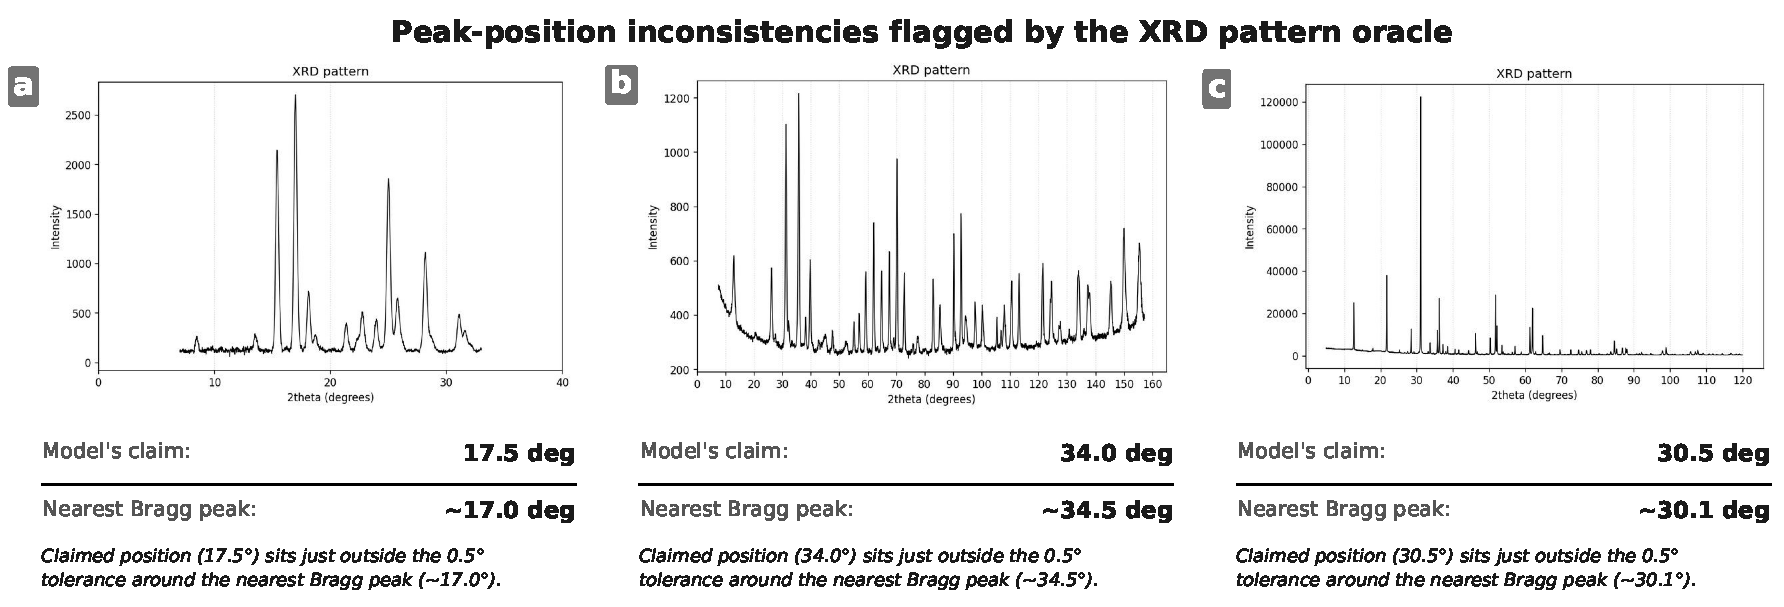
\includegraphics[width=\linewidth]{new_xrd_oracle_figure.pdf}
%\caption{\textbf{Peak-position inconsistencies flagged by the diffraction oracle.} Three
%real, human-confirmed oracle-fired cases: the model's claimed $2\theta$ position, the
%nearest genuine Bragg reflection in the same real diffractogram, and the resulting
%tolerance violation. All three claims sit just outside the oracle's $0.5^\circ$ tolerance
%window around a real peak, consistent with the tolerance-driven false-positive pattern
%described above.}
%\label{fig:xrd-oracle-examples}
%\end{figure}

%\begin{figure}[t]
%\centering
%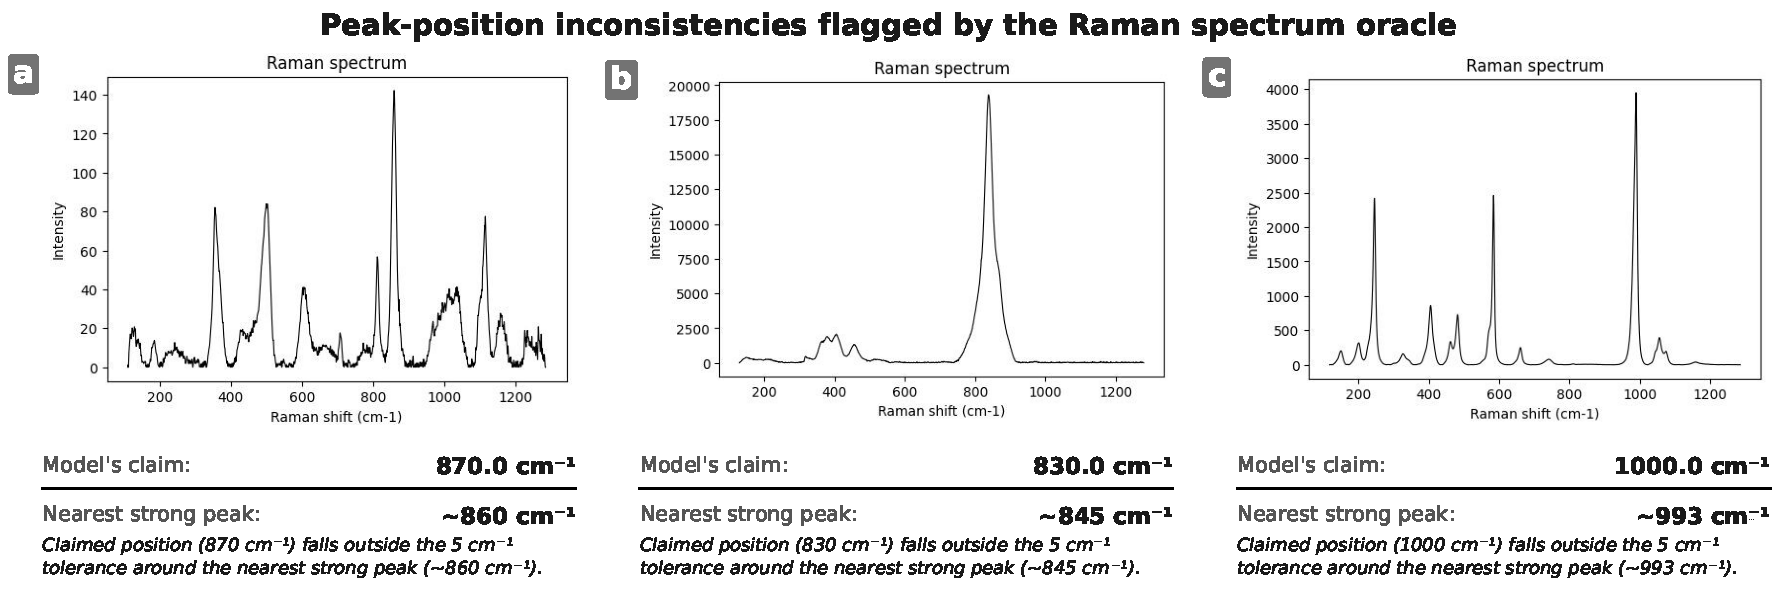
\includegraphics[width=\linewidth]{new_raman_oracle_figure.pdf}
%\caption{\textbf{Peak-position inconsistencies flagged by the Raman spectrum oracle.}
%Three real, human-confirmed oracle-fired cases: the model's claimed Raman shift, the
%nearest genuine strong peak in the same real spectrum, and the resulting tolerance
%violation. All three claims sit just outside the oracle's %$5\,\mathrm{cm}^{-1}$ tolerance
%window around a real peak, the same root cause identified for 34 of 36 %(94\%) of the
%revised spectrum oracle's false positives.}
%\label{fig:raman-oracle-examples}
%\end{figure}

%\begin{figure}[t]
%\centering
%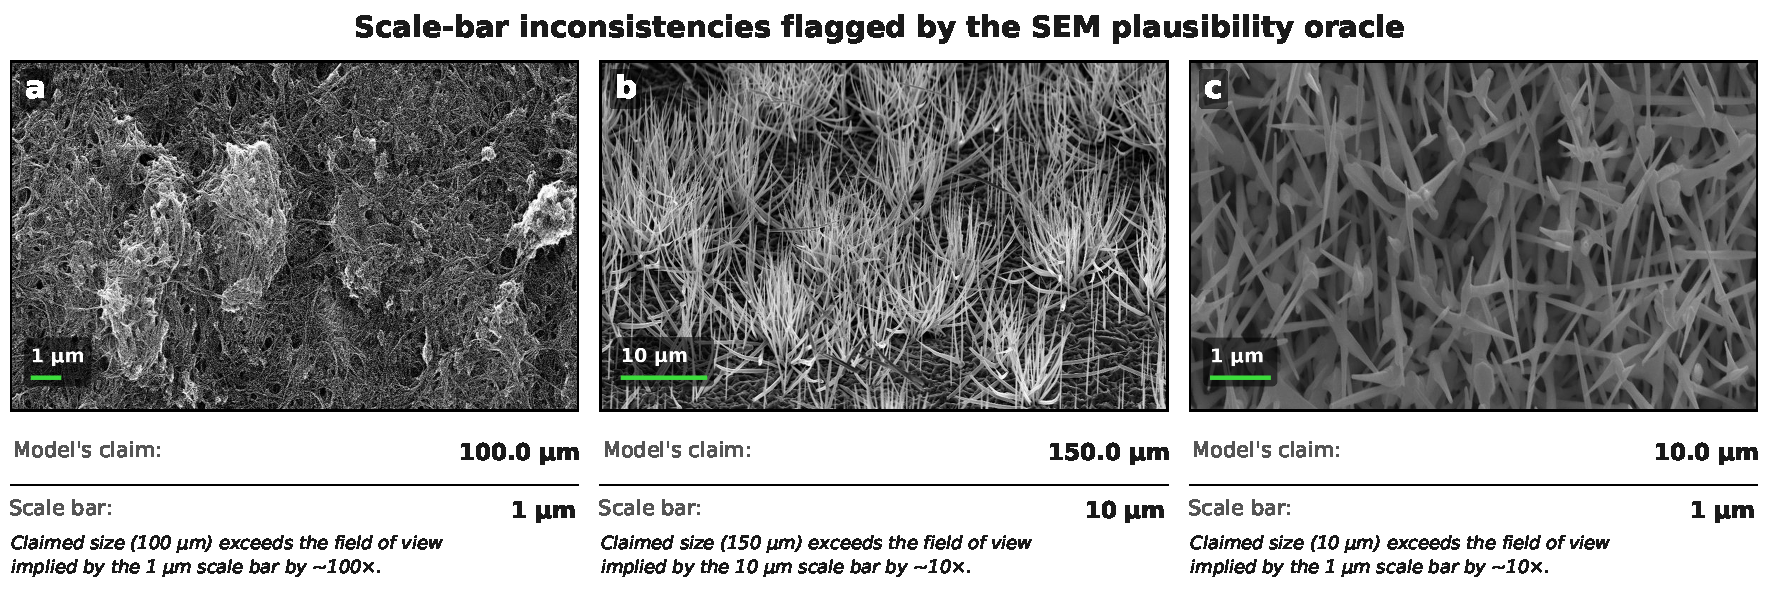
\includegraphics[width=\linewidth]{new_sem_oracle_figure.pdf}
%\caption{\textbf{Scale-bar inconsistencies flagged by the microscopy oracle.} Three real,
%human-confirmed oracle-fired cases: the model's claimed feature size against the real,
%burned-in scale bar of the same NFFA-EUROPE micrograph. Claimed sizes exceed the field of
%view the scale bar implies by roughly $10$--$100\times$, consistent with the scale-bar
%unit and scale-factor arithmetic errors that dominate the microscopy violation taxonomy
%(Results).}
%\label{fig:sem-oracle-examples}
%\end{figure}



\begin{figure}[!htbp]
    \centering

    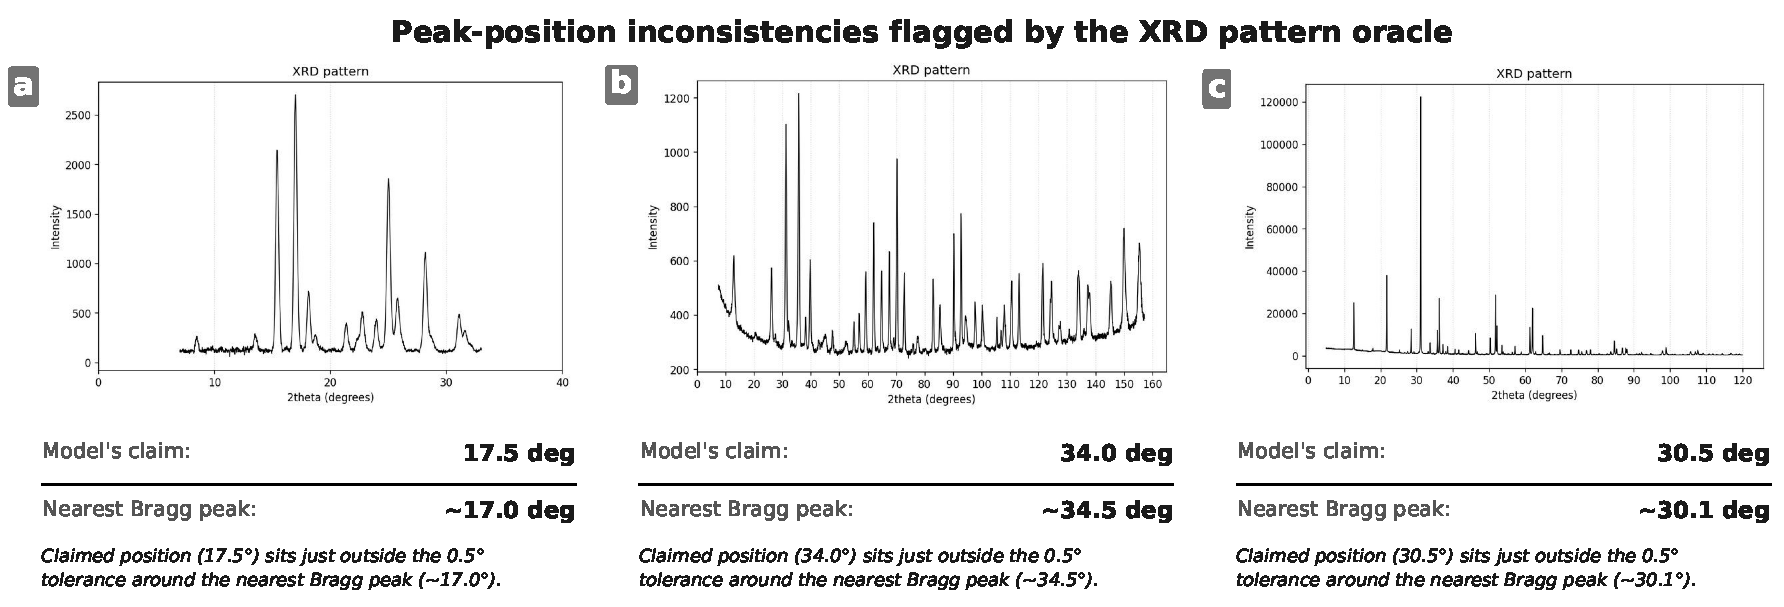
\includegraphics[width=\linewidth,height=0.235\textheight,keepaspectratio]
    {new_xrd_oracle_figure.pdf}

    \vspace{1mm}

    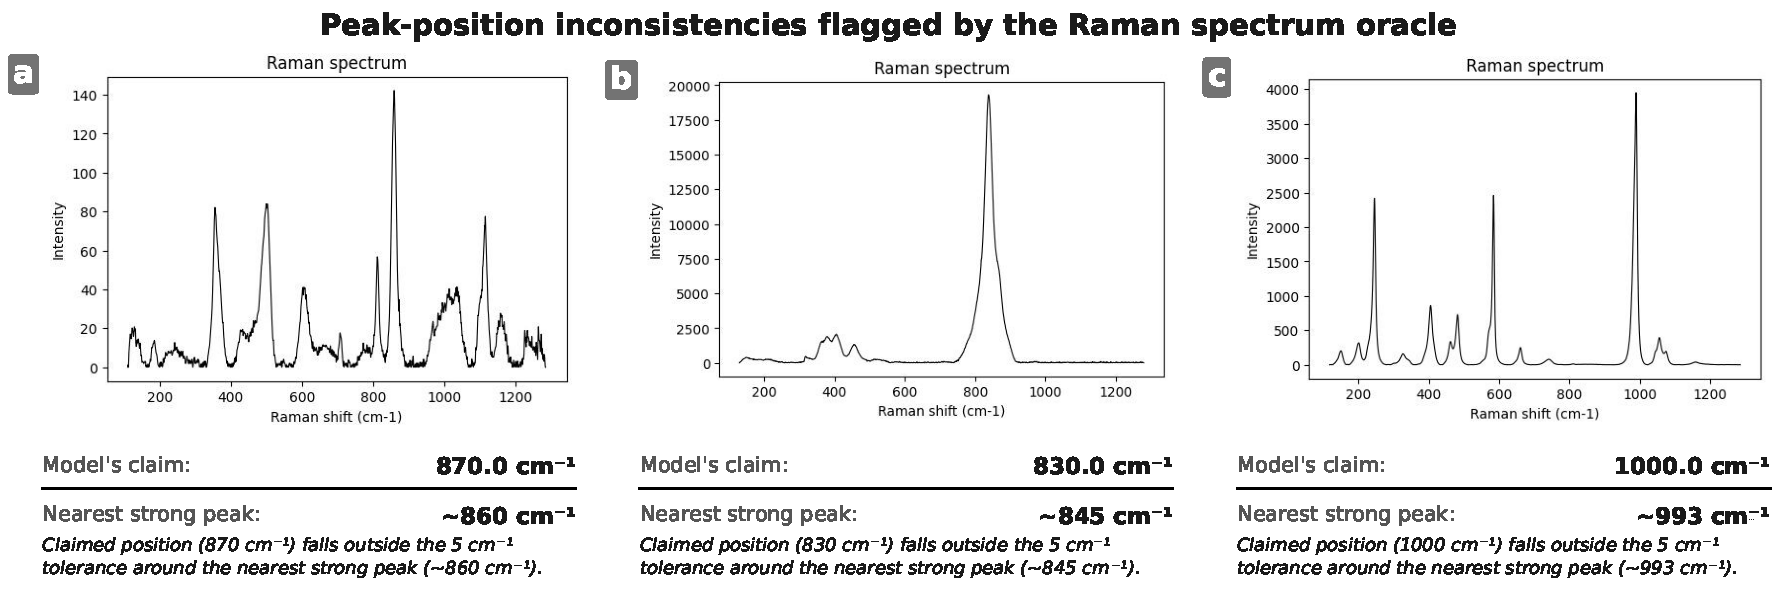
\includegraphics[width=\linewidth,height=0.235\textheight,keepaspectratio]
    {new_raman_oracle_figure.pdf}

    \vspace{1mm}

    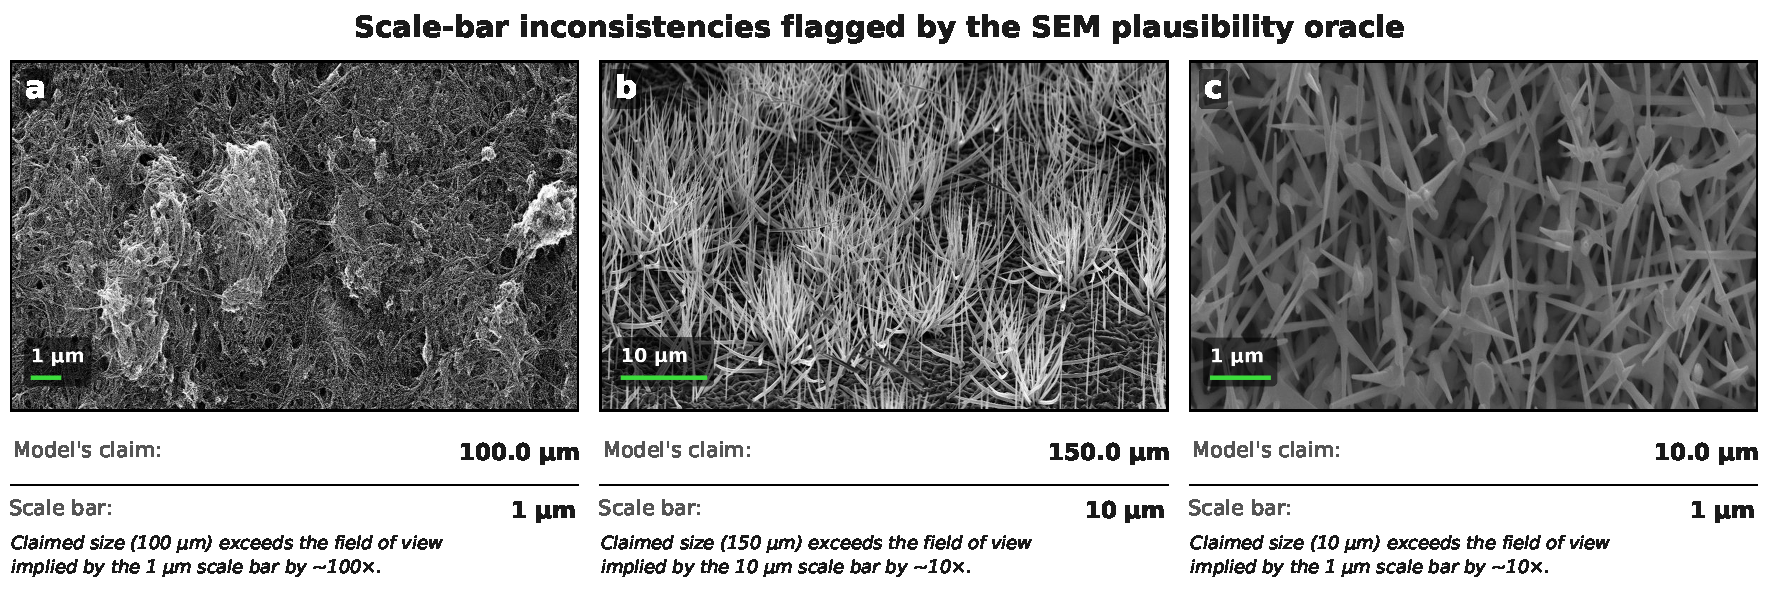
\includegraphics[width=\linewidth,height=0.235\textheight,keepaspectratio]
    {new_sem_oracle_figure.pdf}

    \caption{\justifying\textbf{Representative inconsistencies identified by the multimodal
    oracles.}
    \textbf{a}, X-ray diffraction cases in which the model-reported
    $2\theta$ position lies outside the $0.5^\circ$ tolerance around the nearest
    genuine Bragg reflection.
    \textbf{b}, Raman spectroscopy cases in which the model-reported Raman shift
    exceeds the $5\,\mathrm{cm}^{-1}$ tolerance relative to the nearest genuine
    spectral peak.
    \textbf{c}, Microscopy cases in which the model-reported feature size is
    inconsistent with the physical scale indicated by the embedded scale bar,
    producing discrepancies of approximately $10$--$100\times$.
    All examples are human-confirmed oracle activations and illustrate
    representative tolerance, unit-conversion, and scale-factor failure modes.}

    \label{fig:oracle-examples}
\end{figure}



\begin{table}[t]
\centering
\caption{\justifying\DIFdelbeginFL \DIFdelFL{\textbf{Oracle validity.} }\DIFdelendFL \DIFaddbeginFL \DIFaddFL{\textbf{Oracle validity and audited precision.} }\DIFaddendFL The positive-control
false-negative rate is the maximum across three planted violation rates (10\%, 30\%, and 50\%);
all three rates yielded 0.0000 for every oracle family\DIFaddbeginFL \DIFaddFL{\rev{, which measures completeness on the
injected violation types only}}\DIFaddendFL . Audited precision is the fraction of oracle-fired cases from
Qwen2.5-VL-7B and Gemini 2.5 Flash Lite outputs that human review confirmed as genuine
violations of the stated constraint rather than parsing or oracle artifacts\DIFdelbeginFL \DIFdelFL{. The spectrum result reflects the revised
local-maximum-with-prominence oracle (Methods), evaluated over all 495 oracle-fired cases; the pre-revision result (72.8\%, $n=103$) is reported only for transparency. The three Materials Project-grounded results were
obtained using the final operational definitions: near-hull classification, computed band-gap classification with an abstention band, and
net-magnetization magnitude.}\DIFdelendFL \DIFaddbeginFL \DIFaddFL{\rev{, with Wilson
95\% intervals; $n$ counts decided cases (2 spectrum cases marked unsure are excluded; counting
them either way gives 92.3--92.7\%). Every audit was sampled and judged under the final oracle
definitions used for all reported results (Methods): spectrum responses were collected once and the fired
set re-scored with the final oracle before the audit, and DFT responses were re-collected under the final
definitions before the audit; the diffraction and microscopy audits were carried out in July 2026 and the others in August 2026. Sources: NFFA, NFFA-EUROPE; MP, Materials Project.
$^{a}$Final stability oracle with the near-hull abstention band: the 50 audited cases with
$0<E_{\mathrm{hull}}\le0.05$ eV\,atom$^{-1}$ are not scored; under the original rule the audit gave 95.3\%
[89.5, 98.0] ($n=107$). Consensus: a second annotator, blind to the first labels, re-labelled a random
subsample of 30 audited cases per family stratified by the first annotator's verdict, and the two annotators
adjudicated together every case on which they disagreed (24 in total); the consensus precision is weighted back
to the audited population by stratum, with 95\% intervals from per-stratum Jeffreys posteriors (30 subsampled
cases per family; $^{b}$14, the subsampled stability cases scored under the final oracle). Agreement statistics and the oracle-silent audit are in Supplementary Table~S8.
The full audits were performed by one annotator (R.K.).}}\DIFaddendFL }
\label{tab:exp1}
{\scriptsize\DIFdelbeginFL %DIFDELCMD < \setlength{\tabcolsep}{5pt}%%%
\DIFdelendFL \DIFaddbeginFL \setlength{\tabcolsep}{2.5pt}\DIFaddendFL \renewcommand{\arraystretch}{1.12}
\DIFdelbeginFL %DIFDELCMD < \begin{tabular}{l l S[table-format=1.4] c}
%DIFDELCMD < \toprule
%DIFDELCMD < Oracle family & Data source & {FN rate} & {Audited precision} \\
%DIFDELCMD < \cmidrule(lr){3-3}\cmidrule(lr){4-4}
%DIFDELCMD < & & {\itshape positive control} & {\itshape human audit} \\
%DIFDELCMD < \midrule
%DIFDELCMD < \multicolumn{4}{l}{\itshape Geometric oracles (gate passed)}\\
%DIFDELCMD < Diffraction (XRD)       & opXRD                & 0.0000 & 77.2\%\ \ ($n{=}101$) \\
%DIFDELCMD < Microscopy (SEM)        & NFFA-EUROPE          & 0.0000 & 88.6\%\ \ ($n{=}105$) \\
%DIFDELCMD < Spectra (Raman)         & RRUFF                & 0.0000 & 92.7\%\ \ ($n{=}495$)$^{\dagger}$ \\
%DIFDELCMD < \addlinespace
%DIFDELCMD < \multicolumn{4}{l}{\itshape DFT-grounded oracles}\\
%DIFDELCMD < Stability (hull)        & Materials Project    & 0.0000 & 95.3\%\ \ ($n{=}107$) \\
%DIFDELCMD < Metallicity (band gap)  & Materials Project    & 0.0000 & 94.7\%\ \ ($n{=}114$) \\
%DIFDELCMD < Magnetism (magnitude)   & Materials Project    & 0.0000 & 92.2\%\ \ ($n{=}115$) \\
%DIFDELCMD < \bottomrule
%DIFDELCMD < \end{tabular}%%%
\DIFdelendFL \DIFaddbeginFL \begin{tabular}{l l S[table-format=1.4] c c}
\toprule
Oracle family & Source & {FN rate} & \multicolumn{2}{c}{Audited precision, \% [95\% CI]} \\
\cmidrule(lr){3-3}\cmidrule(lr){4-5}
& & {\itshape positive control} & {\itshape one annotator ($n$)} & \rev{\itshape two-annotator consensus} \\
\midrule
\multicolumn{5}{l}{\itshape Geometric oracles}\\
Diffraction & opXRD & 0.0000 & 77.2 \rev{[68.1, 84.3]} (101) & \rev{60.2 [44.1, 75.4]} \\
Microscopy & NFFA       & 0.0000 & 88.6 \rev{[81.1, 93.3]} (105) & \rev{88.6 [81.8, 93.9]} \\
Raman spectra & RRUFF & 0.0000 & 92.7 \rev{[90.1, 94.7]} (493) & \rev{60.8 [43.6, 76.3]} \\
\addlinespace
\multicolumn{5}{l}{\itshape DFT-grounded oracles}\\
Stability & MP & 0.0000 & \rev{100 [93.7, 100] (57)$^{a}$} & \rev{100 [84.3, 100]$^{b}$} \\
Metallicity & MP & 0.0000 & 94.7 \rev{[89.0, 97.6]} (114) & \rev{94.7 [86.8, 97.0]} \\
Magnetism & MP & 0.0000 & 92.2 \rev{[85.8, 95.8]} (115) & \rev{91.4 [79.9, 96.5]} \\
\bottomrule
\end{tabular}\DIFaddendFL }
\end{table}
\DIFdelbegin %DIFDELCMD < {\scriptsize %%%
\DIFdel{$^{\dagger}$Revised oracle (genuine local-maximum-with-prominence check);
supersedes an earlier pre-revision figure of 72.8\% ($n=103$), see Results.}%DIFDELCMD < }
%DIFDELCMD < %%%
\DIFdelend 

\subsection*{Physical consistency of current models}
We measure the Physical-Consistency Rate and per-constraint-type violation rates for
the four originally evaluated models, four later-generation frontier or open models, and
one flagship-tier addition
across diffraction, microscopy, spectra, and
DFT-grounded constraints, separately for image (VLM) and structure or text (LLM)
inputs (Table~\ref{tab:main}, Fig.~\ref{fig:results}a)\DIFdelbegin \DIFdel{, $n=30$ items per (model, constraint-type) cell per seed, $S=3$ seeds
pooled per cell (4}%DIFDELCMD < {%%%
\DIFdel{,}%DIFDELCMD < }%%%
\DIFdel{472 checkable records in total across the nine models). These numbers
supersede an earlier pass: the spectrum oracle was revised mid-project from a
windowed-maximum check to a genuine-local-maximum-with-prominence check (Methods), which
lowered every model's spectra column substantially, and the magnetism oracle was
redesigned to a per-atom-normalized magnitude check that never compares sign (Methods);
both changes are oracle corrections, not model regressions, and every number below
reflects the corrected oracles. }\DIFdelend \DIFaddbegin \DIFadd{\rev{. Each (model, constraint-type) cell
sends 30 items per seed to the model, with $S=3$ seeds (90 items per cell); 4{,}334 of these
responses are scored across the nine models. For the image constraint types all nine models
receive the same items in each seed, so their comparisons are paired; for the DFT constraint
types each model and seed draws its own block of materials, so those comparisons are unpaired.
Not every attempted item can be scored. On diffraction, 64 of the 90 items per cell have a
reference pattern the oracle can use (the rest lack a usable structure); on metallicity, 1--8
items per cell fall in the oracle's abstention band, and on stability 11--19 items per cell are
near-hull materials, which the final stability oracle does not score (Methods). Within the items the oracle can score, the
share of responses that state a checkable quantity (coverage) is at least 0.93 in every cell
except GPT-4o on spectra (0.49; Supplementary Table~S2).} }\DIFaddend Overall PCR ranges from \DIFdelbegin \DIFdel{0.555
(Qwen3-VL-8B-Instruct) to 0.774 (GPT-5.6-Terra)}\DIFdelend \DIFaddbegin \DIFadd{\rev{0.556
(Qwen3-VL-8B-Instruct) to 0.778 (GPT-5.6-Sol, with GPT-5.6-Terra at 0.777)}}\DIFaddend ; models are
markedly more consistent on microscopy (0.67--1.00) than on spectra (0.07--0.83) or
diffraction (0.47--0.82), and the DFT-grounded column is more tightly clustered
(\DIFdelbegin \DIFdel{0.64--0.74}\DIFdelend \DIFaddbegin \DIFadd{\rev{0.65--0.76}}\DIFaddend ) than any single geometric constraint\DIFdelbegin \DIFdel{, without one constraint type standing
out as uniformly hardest once the corrected oracles are applied. The later-released API models do not uniformly outperform their
earlier siblings: GPT-5.6-Terra improves clearly over GPT-4o
overall (0.774 vs.\ 0.687, bootstrap 95\% CIs $[0.736,0.810]$ vs.\ $[0.643,0.728]$, not
overlapping), but Claude Opus 4.6 does not improve over Claude Sonnet 4.5 (0.655 vs.\
0.656, CIs overlapping), and the reasoning-mode Qwen3-VL-8B-Thinking does not improve over
its non-reasoning sibling (0.579 vs.\ 0.555, CIs overlapping). Explicit reasoning
mode alone therefore does not reliably raise PCR in this sample. The locally run model is the weakest on microscopy
(0.667, 95\% CI $[0.563,0.759]$); six of the other seven models exceed it with
non-overlapping intervals (0.885--1.000), while Qwen3-VL-8B-Instruct at 0.802
($[0.709,0.884]$) does not separate from it. }\DIFdelend \DIFaddbegin \DIFadd{\rev{.}
}

\DIFadd{\rev{Because PCR excludes responses that state no checkable quantity, a model could in
principle raise its score by stating less. We therefore also scored every cell under two
alternative conventions: counting a non-checkable response as a violation (penalised) and as
consistent (lenient). The overall ordering of the nine models is nearly unchanged (Kendall
$\tau=0.83$ between the reported and penalised conventions and $1.00$ between the reported and
lenient ones); the main change is GPT-4o, from third to fifth under the penalised
convention, because of its low coverage on spectra (Supplementary Table~S2).}
}

\DIFadd{\rev{We test model differences at the item level rather than by comparing interval overlap:
exact McNemar tests on the paired image-arm items, Fisher exact tests on the unpaired DFT items,
and, for overall PCR, a bootstrap that resamples paired items jointly and DFT items within
model (Methods). Holm correction is applied within each family of comparisons (Supplementary
Table~S3). GPT-5.6-Terra exceeds GPT-4o overall by 0.072 (95\% CI $[0.018,0.125]$, Holm
$p=0.045$). Claude Opus 4.6 versus Claude Sonnet 4.5 ($-0.003$, $[-0.050,0.044]$),
Qwen3-VL-8B-Thinking versus Qwen3-VL-8B-Instruct ($+0.034$, $[-0.016,0.083]$) and
GPT-5.6-Sol versus GPT-5.6-Terra ($+0.002$, $[-0.042,0.046]$) are not significant. With
roughly 500 checkable items per model, the smallest overall difference the design detects with
80\% power is 0.064--0.079 depending on the pair, so these three comparisons exclude only
differences larger than about 0.07; they do not show that the models are equivalent. Across all
36 model pairs, 18 differences in overall PCR survive Holm correction; within single
constraint types the detectable difference is 0.11--0.20, so most per-type rankings are not
resolved. On microscopy, the locally run Qwen2.5-VL-7B is the weakest model (0.667, 95\% CI
$[0.563,0.759]$), and seven of the other eight models exceed it after Holm correction (paired
differences $+0.22$ to $+0.33$), while Qwen3-VL-8B-Instruct ($+0.14$, Holm $p=0.12$) does not.} }\DIFaddend We do not
\DIFdelbegin \DIFdel{yet }\DIFdelend know whether the gap reflects genuine scale-bar-reading skill or a difference in how each model handles the
info-bar layout variety in the source micrographs, and do not claim more than the
measured difference. The high absolute microscopy rates should also be read against the
looseness of this oracle, which flags only feature sizes exceeding the field of view (a
necessary, not sufficient, condition), so a near-ceiling rate partly reflects an easily
satisfied check. \DIFaddbegin \DIFadd{\rev{Diffraction comparisons in particular should be treated as provisional:
the diffraction ranking changes both when the oracle tolerance is varied and when the prompt is
paraphrased (Methods).}
}\DIFaddend 

\DIFaddbegin \DIFadd{\rev{The DFT column is also sensitive to class composition. The sampled materials are
imbalanced (for stability, only 3--9 of the 70--79 scored materials per model lie on the hull), so a
model that defaults to the majority answer scores well on pooled PCR. Qwen2.5-VL-7B reaches a pooled
stability PCR of 0.917 but answers none of its 4 on-hull materials consistently, a class-balanced rate
of 0.485, whereas GPT-5.6-Terra has the lowest pooled stability PCR (0.653) but a class-balanced rate of
0.814 (Supplementary Table~S4); with so few on-hull materials per model, these class-balanced rates are
imprecise. The ordering of models on the DFT constraint types therefore depends on whether PCR is pooled
or class-balanced, and we report both. To make the DFT comparisons paired as well, we evaluated the
models on one common item set of 90 materials per DFT constraint type, drawn 45 from each reference
class (Supplementary Table~S6); for stability, 34 of the 45 near-hull draws fall in the band the final
oracle does not score, leaving 56 scored materials (11 on the hull, 45 above it). Eight models are
included; Qwen3-VL-8B-Thinking could not be run because its provider endpoint had been withdrawn by the
time of this analysis, and the locally run Qwen2.5-VL-7B was run on CPU in single precision, because no
GPU with bfloat16 support was available then. On this paired set, restricted to the DFT constraint
types, none of the comparisons stated above is significant: GPT-5.6-Terra versus GPT-4o $+0.021$ (95\% CI
$[-0.042,0.085]$), Claude Opus 4.6 versus Claude Sonnet 4.5 $+0.021$ ($[-0.030,0.072]$) and GPT-5.6-Sol
versus GPT-5.6-Terra $+0.030$ ($[-0.013,0.072]$); 3 of the 28 model pairs differ after Holm correction,
all of them Gemini 2.5 Flash Lite scoring lower. The difference between GPT-5.6-Terra and GPT-4o in the
main evaluation therefore comes from the image constraint types, chiefly spectra. The balanced set also
shows a shared failure that the imbalanced sample hid: every model is far less consistent on
computed-metallic compositions (PCR 0.21--0.40) than on gapped ones (0.84--0.96), that is, models
default to calling a composition non-metallic.}
}

\DIFaddend \begin{table}[t]
\centering
\caption{\justifying Main evaluation: Physical-Consistency Rate by constraint type and overall,
\DIFdelbeginFL \DIFdelFL{$n=30$ items }\DIFdelendFL \DIFaddbeginFL \DIFaddFL{\rev{over the checkable responses among 30 attempted items} }\DIFaddendFL per (model, constraint-type) cell per seed, $S=3$ seeds pooled per cell
(bootstrap 95\% CIs omitted from this compact view; see Supplementary Table~S1 for the
full per-cell confidence intervals \DIFaddbeginFL \DIFaddFL{\rev{and checkable counts, Supplementary Table~S2 for coverage
and alternative conventions, Supplementary Table~S3 for paired, Holm-corrected model comparisons,
and Supplementary Table~S4 for class-balanced DFT rates}}\DIFaddendFL , and the Methods for why $\rho_t=1-\mathrm{PCR}$ here). DFT column combines the stability, metallicity,
and magnitude constraint types\DIFaddbeginFL \DIFaddFL{\rev{; near-hull stability materials are not scored (Methods; the original
rule's values are in Supplementary Table~S7)}}\DIFaddendFL .  The first four rows are the
originally evaluated models; the next four are the later-generation refresh
(Methods, Baselines subsection). $^{\ddagger}$GPT-5.6-Sol is OpenAI's flagship tier, added
to test whether it exceeds the balanced-tier GPT-5.6-Terra \DIFdelbeginFL \DIFdelFL{above }\DIFdelendFL within the same
generation; \DIFdelbeginFL \DIFdelFL{its All-column bootstrap 95\% CI, $[0.731,0.806]$, overlaps Terra's
$[0.736,0.810]$, so flagship does not separate from balanced despite leading on
diffraction alone }\DIFdelendFL \DIFaddbeginFL \DIFaddFL{\rev{the overall difference is $+0.002$ (95\% CI $[-0.042,0.046]$), not significant, so
the design detects no difference between flagship and balanced tier larger than about 0.07}
}\DIFaddendFL (Discussion). \DIFaddbeginFL \DIFaddFL{\rev{Bold marks the column maximum; it does not imply a significant difference from
the next model.}}\DIFaddendFL }
\label{tab:main}
{\scriptsize\setlength{\tabcolsep}{5pt}\renewcommand{\arraystretch}{1.12}
\DIFdelbeginFL %DIFDELCMD < \begin{tabular}{l *{5}{S[table-format=1.3]}}
%DIFDELCMD < \toprule
%DIFDELCMD < & \multicolumn{5}{c}{Physical-Consistency Rate (higher is more consistent)} \\
%DIFDELCMD < \cmidrule(lr){2-6}
%DIFDELCMD < Model & {Diffraction} & {Microscopy} & {Spectra} & {DFT$^{*}$} & {All$^{*}$} \\
%DIFDELCMD < \midrule
%DIFDELCMD < Qwen2.5-VL-7B \textit{(open)} & 0.500 & 0.667 & 0.148 & 0.685 & 0.565 \\
%DIFDELCMD < Gemini 2.5 Flash Lite & 0.517 & \bfseries 1.000 & 0.278 & 0.641 & 0.622 \\
%DIFDELCMD < GPT-4o                & 0.625 & 0.954 & 0.068 & 0.717 & 0.687 \\
%DIFDELCMD < Claude Sonnet 4.5     & 0.547 & 0.977 & 0.189 & \bfseries 0.736 & 0.656 \\
%DIFDELCMD < \addlinespace
%DIFDELCMD < Claude Opus 4.6            & 0.578 & 0.954 & 0.244 & 0.714 & 0.655 \\
%DIFDELCMD < GPT-5.6-Terra              & 0.797 & 0.951 & \bfseries 0.833 & 0.694 & \bfseries 0.774 \\
%DIFDELCMD < Qwen3-VL-8B-Instruct       & 0.468 & 0.802 & 0.133 & 0.642 & 0.555 \\
%DIFDELCMD < Qwen3-VL-8B-Thinking       & 0.578 & 0.885 & 0.092 & 0.639 & 0.579 \\
%DIFDELCMD < \addlinespace
%DIFDELCMD < GPT-5.6-Sol$^{\ddagger}$   & \bfseries 0.820 & 0.915 & 0.764 & 0.715 & 0.770 \\
%DIFDELCMD < \bottomrule
%DIFDELCMD < \end{tabular}%%%
\DIFdelendFL \DIFaddbeginFL \begin{tabular}{l *{5}{S[table-format=1.3]}}
\toprule
& \multicolumn{5}{c}{Physical-Consistency Rate (higher is more consistent)} \\
\cmidrule(lr){2-6}
Model & {Diffraction} & {Microscopy} & {Spectra} & {DFT$^{*}$} & {All$^{*}$} \\
\midrule
Qwen2.5-VL-7B \textit{(open)} & 0.500 & 0.667 & 0.148 & \rev{0.731} & \rev{0.584} \\
Gemini 2.5 Flash Lite & 0.517 & \bfseries 1.000 & 0.278 & \rev{0.658} & \rev{0.630} \\
GPT-4o                & 0.625 & 0.954 & 0.068 & \rev{0.740} & \rev{0.699} \\
Claude Sonnet 4.5     & 0.547 & 0.977 & 0.189 & \bfseries \rev{0.762} & \rev{0.667} \\
\addlinespace
Claude Opus 4.6            & 0.578 & 0.954 & 0.244 & \rev{0.734} & \rev{0.663} \\
GPT-5.6-Terra              & 0.797 & 0.951 & \bfseries 0.833 & \rev{0.696} & \rev{0.777} \\
Qwen3-VL-8B-Instruct       & 0.468 & 0.802 & 0.133 & \rev{0.649} & \rev{0.556} \\
Qwen3-VL-8B-Thinking       & 0.578 & 0.885 & 0.092 & \rev{0.671} & \rev{0.594} \\
\addlinespace
GPT-5.6-Sol$^{\ddagger}$   & \bfseries 0.820 & 0.915 & 0.764 & \rev{0.727} & \bfseries \rev{0.778} \\
\bottomrule
\end{tabular}\DIFaddendFL }
\end{table}


\subsection*{Accuracy versus consistency}
On three constraint types with a genuine, non-circular accuracy criterion distinct
from the oracle's own tolerance (diffraction: agreement with the single nearest true
peak to $0.1^{\circ}$, versus the oracle's looser $0.5^{\circ}$ tolerance; spectra:
agreement with the nearest real measured peak to $2\,\mathrm{cm}^{-1}$, versus the
oracle's prominence-based check; stability: agreement with the Materials
Project \texttt{is\_stable} label, evaluated separately from the oracle's
operational $0.05\,\mathrm{eV\,atom^{-1}}$ near-hull threshold), we report
accuracy alongside PCR and the four-cell breakdown on the same
\DIFdelbegin \DIFdel{920 items }\DIFdelend \DIFaddbegin \DIFadd{\rev{838 scored items} }\DIFaddend ($n=30$ per (model, constraint-type) cell, $S=3$ seeds\DIFdelbegin \DIFdel{; recomputed directly from
\texttt{experiments/exp3\_results.jsonl}, which supersedes an earlier 918-item run). This
figure is not directly comparable to Supplementary Table~S1's 923 checkable records for the
same four models' diffraction, spectra and stability cells: that table reports Experiment 2's
main PCR sweep, a separately drawn sample for a different purpose, not this accuracy-versus-
consistency analysis; the two are expected to differ and are not a reconciliation target for
each other. }\DIFdelend \DIFaddbegin \DIFadd{\rev{, the four originally evaluated
models; this sample is drawn separately from the main evaluation}). }\DIFaddend Microscopy is excluded: its
prompt elicits only a feature-size claim, so no non-circular accuracy ground truth is
available without a different prompt design. \DIFdelbegin \DIFdel{These numbers reflect the corrected
spectrum oracle (Methods) and supersede an earlier pass in which the gap was reported
differently. Across all 12 (model, constraint-type) cells,
accuracy and PCR disagree on a mean of 22.2\% of items, confirming that PCR is not
answer accuracy under another name (Fig.~\ref{fig:pipeline}b,c). }\DIFdelend \DIFaddbegin \DIFadd{\rev{On the eight diffraction and spectra cells,
accuracy and PCR disagree on a mean of 23.6\% of items, and on stability they coincide
(Fig.~\ref{fig:pipeline}b,c). Part of the diffraction and spectra disagreement is definitional rather
than evidence of reasoning errors that accuracy misses: the accuracy criteria are deliberately tighter
than the oracle tolerances, so the two scores are expected to differ on items that fall between the two
thresholds. What the comparison does establish is that
the two scores measure different properties of the same response, not that PCR detects errors that
accuracy cannot.} }\DIFaddend Diffraction is dominated by items
that are wrong by the tight accuracy criterion yet still oracle-consistent (up to 36
of 62 items in one diffraction cell, gap 58.1\%): models are frequently close enough to satisfy the
oracle's looser tolerance while measurably off the exact peak. \DIFdelbegin \DIFdel{Spectra, under the corrected
oracle, is now dominated by the opposite pattern from before the correction: most
disagreement is items wrong by both criteria (WI) rather than wrong-but-consistent (WC),
so the accuracy-consistency gap for spectra is small (}\DIFdelend \DIFaddbegin \DIFadd{\rev{On spectra, most responses
are wrong by both criteria, so the two scores disagree on few items} (}\DIFaddend 4.2--11.2\% across models)\DIFdelbegin \DIFdel{rather
than the large WC-dominated gap the pre-correction oracle produced; the earlier framing of
spectra as the largest-gap constraint no longer holds under the corrected oracle. Stability
still shows its own distinct pattern, dominated by items that are classified differently by the Materials Project \texttt{is\_stable} label
and the operational near-hull threshold, a direct
consequence of the two definitions of stability disagreeing on a substantial share of real
materials: on a random sample of 3,000 real Materials Project entries, the oracle's
$\epsilon=0.05\,\mathrm{eV\,atom^{-1}}$ tolerance and Materials Project's own strict
\texttt{is\_stable} label disagree on 571 (19.0\%); its gap (18.0--27.8\% across models) is now
comparable to, rather than smaller than, diffraction's. One model (Qwen2.5-VL-7B) shows a raw stability accuracy
of 81/82 (0.988) on the unstable class but 0/8 on the small stable class, the clearest case of the base-rate confound: because the sampled materials skew
toward the unstable class, near-ceiling raw accuracy reflects the base rate rather than
discriminative skill. Balanced accuracy (the mean of per-class accuracy, correcting for
this skew) is 0.494 (Qwen2.5-VL-7B), 0.681 (Gemini 2.5 Flash Lite), 0.476 (GPT-4o), and
0.971 (Claude Sonnet 4.5). Three of four models fall to at or near chance once the
class imbalance is corrected for, and only Claude Sonnet 4.5's apparent skill survives
this correction ($n=90$ per model, 5--8 stable and 82--85 unstable materials per model's
sample).
}\DIFdelend \DIFaddbegin \DIFadd{. \rev{On stability the two scores coincide under the final protocol,
and this is informative in itself. The oracle's $0.05\,\mathrm{eV\,atom^{-1}}$ near-hull threshold and
Materials Project's own \texttt{is\_stable} label (true only on the hull) disagree on 571 of 3,000 real
entries (19.0\%), and every one of those is a near-hull material, $0<E_{\mathrm{hull}}\le0.05$. The final
oracle does not score that band (Methods), so outside it the two definitions agree, and the stability gap
of 18.0--27.8\% reported under the original rule came entirely from the near-hull materials. The stability
arm still shows the base-rate confound: Qwen2.5-VL-7B is accurate on 61 of 62 unstable materials but on
none of the 8 stable ones, so its near-ceiling raw accuracy reflects the base rate rather than
discriminative skill. Balanced accuracy (the mean of per-class accuracy) is 0.492 (Qwen2.5-VL-7B), 0.690
(Gemini 2.5 Flash Lite), 0.492 (GPT-4o) and 0.992 (Claude Sonnet 4.5); two of the four models are at
chance once the imbalance is corrected for ($n=65$--73 scored materials per model, 5--8 of them stable).}
}\DIFaddend 

\DIFaddbegin \DIFadd{\rev{What PCR adds to answer accuracy is therefore not a finer measure of correctness but a
different, label-free property. First, it needs no answer key: it is defined on microscopy and
on net magnetization, where this benchmark has no non-circular accuracy criterion, and on any new
item for which a reference structure, scale bar or computed value exists. Second, it is a floor
rather than a target: a violation is a statement the measurement or the reference calculation
rules out, so a violation is informative about the reasoning that produced it (Fig.~\ref{fig:teaser}c
shows what these violations consist of), whereas an accuracy miss may only reflect reading
precision. Third, because it is a necessary condition, PCR cannot certify that a response is
right; a high PCR with low accuracy, as on diffraction, identifies responses that are physically
admissible but imprecise. We therefore present PCR as a complement to answer accuracy where labels
exist and as a substitute screening signal where they do not, not as a replacement for either.}
}

\DIFaddend \subsection*{Effect of self-verification}
We measure PCR before and after CGSV on identical items and test the change with the
exact paired McNemar test, reporting fixes, regressions, and residual violations
(Table~\ref{tab:cgsv}, Fig.~\ref{fig:results}b), on diffraction and spectra, the two constraint types where
the oracle's feedback is an actionable physical constraint the model can re-examine
without the feedback message itself revealing the answer (a scale-bar violation
message would state the conversion factor outright, and the three DFT claim types are
single-shot binary judgments with no intermediate quantity to reconsider). $n=30$
items per (model, constraint-type) cell, $S=3$ seeds, $K=2$ maximum revision rounds, 545
checkable records in total\DIFdelbegin \DIFdel{(superseding an earlier 555-record pass under the
pre-correction spectrum oracle). CGSV never regresses a previously consistent item: the
regression count $b=0$ in every one of the 8 (model, constraint-type) cells and in the
pooled per-model totals. CGSV significantly }\DIFdelend \DIFaddbegin \DIFadd{. \rev{Because Algorithm~\ref{alg:cgsv} stops at the first round in which no
violation remains, an item that is consistent before revision is never revised. The absence of
regressions in consistency ($b=0$ in every cell) therefore follows from the stopping rule; it
confirms the implementation but is not evidence about the model.} CGSV }\DIFaddend raises PCR for all four models pooled across both
constraint types (Qwen2.5-VL-7B $0.338\!\to\!0.439$, $p=3.1\times10^{-5}$; Gemini 2.5
Flash Lite $0.521\!\to\!0.632$, $p=2.4\times10^{-4}$; GPT-4o
$0.434\!\to\!0.593$, $p=7.6\times10^{-6}$; Claude Sonnet 4.5 $0.373\!\to\!0.639$,
$p=4.6\times10^{-13}$\DIFdelbegin \DIFdel{); under the corrected spectrum oracle, absolute PCR is lower
throughout (tracking the main table's spectrum collapse) but the relative gain and its
significance are, if anything, stronger for every model than under the earlier oracle}\DIFdelend \DIFaddbegin \DIFadd{\rev{; all survive Holm correction})}\DIFaddend .
Residual violations remain in every cell after $K=2$ rounds (roughly 40--90\% of
items \DIFdelbegin \DIFdel{under the stricter corrected spectrum oracle}\DIFdelend \DIFaddbegin \DIFadd{\rev{on spectra}}\DIFaddend ), so CGSV \DIFdelbegin \DIFdel{measurably improves }\DIFdelend \DIFaddbegin \DIFadd{reduces }\DIFaddend but does not eliminate violations\DIFdelbegin \DIFdel{, a positive
control on the oracles, not a guarantee of full correction.
Because CGSV is scored by the same oracles that supply its feedback, a rise in PCR is
consistent both with the model correcting the flagged physics and with it retracting or
hedging the flagged claim; separating these requires the number of checkable claims each
chain exposes before and after CGSV. We checked this directly: this benchmark's
single-claim-per-item design means every one of the 545 items exposed exactly one
checkable claim in every round it reached, before and after revision ($k_i=1$ for all $i$,
confirmed by comparing each item's number of recorded claim values against its number of
revision rounds; zero items exposed fewer claims after CGSV than before). Because $k_i$
never changes, a PCR gain here cannot be explained by the model dropping a checkable claim;
it must reflect the claim's stated value changing to one the oracle judges consistent. This
rules out retraction in the sense of claim removal. It does not rule out retreat: a model
could move to a value that is trivially admissible rather than to the physically right one,
which the oracle, being a necessary-condition check, would accept either way. Distinguishing
those two would require the post-CGSV accuracy of the revised claim. We computed it, applying
the same non-circular accuracy criteria as the accuracy-versus-consistency analysis
($0.1^\circ$ for diffraction, $2\,\mathrm{cm}^{-1}$ for spectra) to each item's final-round
claim: post-CGSV accuracy is 29.8\% on diffraction ($n=252$) and 9.9\% on spectra ($n=293$),
both far below the corresponding post-CGSV PCR (Table~\ref{tab:cgsv}). Most of the CGSV gain
is therefore retreat, not correction: the model moves to a value the oracle's necessary
condition accepts far more often than it moves to the value that is actually right. CGSV
demonstrably reduces oracle-detected violations; this result shows it does not, on the
evidence here, demonstrably improve the underlying physical correctness of the claim. We separately isolate whether this gain is
}\DIFdelend \DIFaddbegin \DIFadd{.
}

\DIFadd{\rev{Because CGSV is scored by the same oracles that supply its feedback, a rise in PCR alone cannot
show that revised answers are more correct. Every item exposes exactly one checkable claim in
every round, so a gain cannot come from the model dropping the claim. To see what the revisions
achieve, we scored each item's first-round and final-round claim against the same non-circular
accuracy criteria as the accuracy-versus-consistency analysis ($0.1^\circ$ for diffraction,
$2\,\mathrm{cm}^{-1}$ for spectra) and compared them on the same items (Table~\ref{tab:cgsvacc}).
Accuracy is a property the loop never observes, so unlike consistency it can regress. On spectra
($n=293$) accuracy rises from 5.8\% to 9.9\%: 14 items become accurate and 2 cease to be (exact
McNemar $p=0.004$). Of the 244 spectrum items the oracle flagged and the model revised, 48 cleared
the oracle; 11 of these moved to the accurate value and 37 to a value the oracle admits but that
is not within the accuracy tolerance, and the remaining 196 stayed inconsistent.
On diffraction ($n=245$; 7 items whose reference pattern could not be computed are omitted) accuracy
rises from 22.9\% to 28.6\%: 14 items become accurate and none ceases to be (exact McNemar $p=0.0001$).
Of the 79 diffraction items the oracle flagged and the model revised, 41 cleared the oracle; 14 of these
moved to the accurate value and 27 to an admissible but inexact one, and 38 stayed inconsistent. Revisions that clear
the oracle therefore mostly move a claim into the physically admissible region rather than onto the
exact value, while also producing a small but significant net gain in correctness. The evidence
supports this narrower statement, not a claim that CGSV corrects the underlying physics in general.}
}

\DIFadd{\rev{We separately ask whether the gain is}
}\DIFaddend attributable to the oracle signal specifically, or to extra inference-time compute alone,
with three controls matched to CGSV's items, models, and decoding
(Baselines subsection): unaided self-refinement (the model is told to double-check its
answer with no oracle feedback) shows no significant change (before $0.349$, after $0.339$, $n=542$, $b=34$, $c=29$, $p=0.615$);
generic equal-compute re-prompting (the model is simply asked to reconsider) likewise shows
no significant change (before $0.358$, after $0.342$, $n=562$, $b=24$, $c=15$, $p=0.20$)\DIFdelbegin \DIFdel{; both controls, unlike CGSV
itself, show nonzero regressions ($b>0$). }\DIFdelend \DIFaddbegin \DIFadd{. \rev{Both
controls revise every item, including those already consistent, so their nonzero regression counts
are not comparable with CGSV's structural $b=0$; the comparison that matters is the net change,
which is significant for CGSV and absent for both controls.} }\DIFaddend Best-of-3 independent resampling gives a
random-pick PCR of $0.363$ and an oracle-oracle upper bound (best of 3) of $0.419$
($n=614$). Both fall below CGSV's oracle-guided after-PCR for every model, though the
margin over the weakest, Qwen2.5-VL-7B at $0.439$, is only $0.02$, and the resampling run
draws its own item sample, so we do not test the difference. \DIFdelbegin \DIFdel{Together these
controls support attributing CGSV's gain to the physical-consistency signal specifically,
not to generic self-reflection or additional sampling at equal compute.
}\DIFdelend \DIFaddbegin \DIFadd{\rev{These controls show that the PCR gain
is not reproduced by generic self-reflection or by extra sampling at equal compute; they do not
by themselves show that the gain reflects better physics, which is what the paired correctness
analysis above addresses.}
}\DIFaddend 

\begin{table}[t]
\centering
\caption{\justifying Effect of Constraint-Grounded Self-Verification, pooled across diffraction
and spectra, $n=30$ items per (model, constraint-type) cell, $S=3$ seeds, $K=2$ rounds\DIFdelbeginFL \DIFdelFL{,
under the corrected spectrum oracle (Methods)}\DIFdelendFL .
$\Delta$: PCR gain (after minus before); $b$: regressions (before-consistent,
after-inconsistent); $c$: fixes (before-inconsistent, after-consistent); $p$: exact
two-sided McNemar test on $(b,c)$; $p_{\mathrm{Holm}}$: Holm-Bonferroni-adjusted $p$ over
this table's 6-test family (Methods, Statistics paragraph\DIFdelbeginFL \DIFdelFL{;
\texttt{experiments/exp15\_multiplicity\_correction.py}}\DIFdelendFL ). All four CGSV effects survive
this \DIFdelbeginFL \DIFdelFL{strictest }\DIFdelendFL correction; both controls remain non-significant. \DIFaddbeginFL \DIFaddFL{\rev{For CGSV, $b=0$ follows from the stopping
rule (an item consistent before revision is never revised); the controls revise every item, so
their $b$ is not comparable. Paired changes in correctness are in Table~\ref{tab:cgsvacc}.}}\DIFaddendFL }
\label{tab:cgsv}
{\scriptsize\DIFdelbeginFL %DIFDELCMD < \setlength{\tabcolsep}{4pt}%%%
\DIFdelendFL \DIFaddbeginFL \setlength{\tabcolsep}{3.4pt}\DIFaddendFL \renewcommand{\arraystretch}{1.12}
\DIFdelbeginFL %DIFDELCMD < \begin{tabular}{l S[table-format=1.3] S[table-format=1.3] S[table-format=+1.3] S[table-format=1.0] S[table-format=2.0] c c}
%DIFDELCMD < \toprule
%DIFDELCMD < & \multicolumn{3}{c}{PCR} & \multicolumn{2}{c}{Discordant} & & \\
%DIFDELCMD < \cmidrule(lr){2-4}\cmidrule(lr){5-6}
%DIFDELCMD < Model & {before} & {after} & {$\Delta$} & {$b$} & {$c$} & {$p$} & {$p_{\mathrm{Holm}}$} \\
%DIFDELCMD < \midrule
%DIFDELCMD < Qwen2.5-VL-7B         & 0.338 & 0.439 & 0.101 & 0 & 16 & $3.1\times10^{-5}$ & $1.2\times10^{-4}$ \\
%DIFDELCMD < Gemini 2.5 Flash Lite & 0.521 & 0.632 & 0.111 & 0 & 13 & $2.4\times10^{-4}$ & $7.3\times10^{-4}$ \\
%DIFDELCMD < GPT-4o                & 0.434 & 0.593 & \bfseries 0.159 & 0 & 18 & $7.6\times10^{-6}$ & $3.8\times10^{-5}$ \\
%DIFDELCMD < Claude Sonnet 4.5     & 0.373 & 0.639 & \bfseries 0.266 & 0 & 42 & $4.6\times10^{-13}$ & $2.7\times10^{-12}$ \\
%DIFDELCMD < \midrule
%DIFDELCMD < \multicolumn{8}{l}{\itshape Mechanism-isolation controls (pooled across models, both constraint types)}\\
%DIFDELCMD < Self-refinement (no oracle) & 0.349 & 0.339 & -0.010 & 34 & 29 & 0.615 & 0.615 \\
%DIFDELCMD < Generic re-prompting        & 0.358 & 0.342 & -0.016 & 24 & 15 & 0.20 & 0.399 \\
%DIFDELCMD < \bottomrule
%DIFDELCMD < \end{tabular}%%%
\DIFdelendFL \DIFaddbeginFL \begin{tabular}{l S[table-format=1.3] S[table-format=1.3] S[table-format=+1.3] S[table-format=2.0] S[table-format=2.0] c c}
\toprule
& \multicolumn{3}{c}{PCR} & \multicolumn{2}{c}{Discordant} & & \\
\cmidrule(lr){2-4}\cmidrule(lr){5-6}
Model & {before} & {after} & {$\Delta$} & {$b$} & {$c$} & {$p$} & {$p_{\mathrm{Holm}}$} \\
\midrule
Qwen2.5-VL-7B         & 0.338 & 0.439 & 0.101 & 0 & 16 & $3.1\times10^{-5}$ & $1.2\times10^{-4}$ \\
Gemini 2.5 Flash Lite & 0.521 & 0.632 & 0.111 & 0 & 13 & $2.4\times10^{-4}$ & $7.3\times10^{-4}$ \\
GPT-4o                & 0.434 & 0.593 & \bfseries 0.159 & 0 & 18 & $7.6\times10^{-6}$ & $3.8\times10^{-5}$ \\
Claude Sonnet 4.5     & 0.373 & 0.639 & \bfseries 0.266 & 0 & 42 & $4.6\times10^{-13}$ & $2.7\times10^{-12}$ \\
\midrule
\multicolumn{8}{l}{\itshape Mechanism-isolation controls (pooled across models, both constraint types)}\\
Self-refinement (no oracle) & 0.349 & 0.339 & -0.010 & 34 & 29 & 0.615 & 0.615 \\
Generic re-prompting        & 0.358 & 0.342 & -0.016 & 24 & 15 & 0.20 & 0.399 \\
\bottomrule
\end{tabular}\DIFaddendFL }
\end{table}

\DIFaddbegin \begin{table}[t]
\DIFaddFL{\revon}\centering
\caption{\justifying \DIFaddFL{Paired change in answer correctness before and after CGSV, on the same items as
Table~\ref{tab:cgsv}. Accuracy uses the non-circular criteria of the accuracy-versus-consistency
analysis (diffraction: within $0.1^\circ$ of the nearest reference reflection; spectra: within
$2\,\mathrm{cm}^{-1}$ of the nearest detected local maximum), applied to each item's first-round
and final-round claim (accuracy before$\to$after). L/G: items that stop (lost) or start (gained) being
accurate; $p$: exact two-sided McNemar test on (L, G). Rev.: items the oracle flagged at round 1 and the
model revised; of these, A cleared the oracle with an accurate value, Ad cleared it with an admissible
value outside the accuracy tolerance, and U were still flagged after $K=2$ rounds.}}
\label{tab:cgsvacc}
{\scriptsize\setlength{\tabcolsep}{2.5pt}\renewcommand{\arraystretch}{1.12}
\begin{tabular}{l l r c c r r c}
\toprule
Constraint & Model & $n$ & Accuracy & L/G & $p$ & Rev. & A/Ad/U \\
\midrule
Spectra & Qwen2.5-VL-7B & 89 & 0.067$\to$0.101 & 0/3 & 0.25 & 80 & 3/9/68 \\
 & Gemini 2.5 F.\ Lite & 69 & 0.043$\to$0.072 & 0/2 & 0.50 & 49 & 2/6/41 \\
 & GPT-4o & 45 & 0.044$\to$0.044 & 1/1 & 1.00 & 40 & 0/4/36 \\
 & Claude Sonnet 4.5 & 90 & 0.067$\to$0.144 & 1/8 & 0.039 & 75 & 6/18/51 \\
 & \textit{pooled} & 293 & 0.058$\to$0.099 & 2/14 & 0.004 & 244 & 11/37/196 \\
\addlinespace
Diffraction & Qwen2.5-VL-7B & 66 & 0.303$\to$0.318 & 0/1 & 1.00 & 24 & 1/3/20 \\
 & Gemini 2.5 F.\ Lite & 47 & 0.213$\to$0.255 & 0/2 & 0.50 & 7 & 2/3/2 \\
 & GPT-4o & 66 & 0.152$\to$0.212 & 0/4 & 0.12 & 24 & 4/10/10 \\
 & Claude Sonnet 4.5 & 66 & 0.242$\to$0.348 & 0/7 & 0.016 & 24 & 7/11/6 \\
 & \textit{pooled} & 245 & 0.229$\to$0.286 & 0/14 & 0.0001 & 79 & 14/27/38 \\
\bottomrule
\end{tabular}}
\end{table}

\DIFaddend \subsection*{Verifier for violation prediction}
We fine-tune Qwen2.5-0.5B-Instruct with LoRA on oracle-derived labels alone (no human
annotation) to predict, from the input description and chain text alone, whether a
physical violation is present, using 2{,}152 real oracle-checked records spanning all
six constraint types collected across the preceding evaluations\DIFdelbegin \DIFdel{(superseding an earlier
2}%DIFDELCMD < {%%%
\DIFdel{,}%DIFDELCMD < }%%%
\DIFdel{416-record pass under the pre-correction spectrum oracle)}\DIFdelend . We report precision,
recall, $F_1$, ROC AUC, and expected calibration error (ECE) on an 80/20
in-distribution split and separately on six held-out-constraint-type splits (train on the
other five constraint types, test on one entirely unseen one). The in-distribution split
is disjoint at the parent source (item \DIFdelbegin \DIFdel{/}\DIFdelend \DIFaddbegin \DIFadd{or }\DIFaddend structure) level, \DIFdelbegin \DIFdel{not the record level: an earlier
pass split at the record level, which let seed replicates and same-chain claims of one item
land on both sides of the split and leaked item identity into the reported in-distribution
number; we rebuilt the dataset to retain a source identifier and re-split so that no source
item appears on both sides}\DIFdelend \DIFaddbegin \DIFadd{\rev{so no source item contributes
records to both sides}}\DIFaddend . In distribution the verifier is a useful
detector \DIFaddbegin \DIFadd{overall }\DIFaddend (precision 0.77, recall 0.71, $F_1=0.74$, AUC $=0.850$, ECE $=0.096$\DIFdelbegin \DIFdel{, close to but
slightly below the pre-fix leaky estimate of AUC $=0.858$, as expected once the leak is
closed).
}\DIFdelend \DIFaddbegin \DIFadd{).
\rev{This pooled figure overstates its usefulness for a given scientific task, for two reasons.
First, the six families have very different violation base rates (19\% for microscopy to 88\%
for spectra in the test split), so a score that only identified the family would already rank
violations above chance: a baseline that assigns each item its family's training-set violation
rate reaches AUC $=0.759$. Second, within single families the verifier's discrimination varies
widely (Table~\ref{tab:verifierfam}): it is strong on microscopy (AUC $0.922$, 95\% CI
$[0.852,0.977]$) and stability ($0.804$, $[0.683,0.903]$), moderate on magnetism ($0.728$,
$[0.562,0.877]$) and diffraction ($0.696$, $[0.493,0.895]$), and not distinguishable from chance on
metallicity ($0.582$, $[0.390,0.775]$) and spectra ($0.513$, $[0.353,0.702]$). The in-distribution
verifier is therefore a useful triage signal for microscopy and stability claims, a weak one for
magnetism and diffraction, and not useful for metallicity or spectra.} }\DIFaddend Its
cross-constraint-type generalization is poor for all six constraint types\DIFdelbegin \DIFdel{under the
source-disjoint split}\DIFdelend : diffraction, microscopy, and stability
are indistinguishable from chance when held out entirely (AUC 0.50, 0.53, and 0.44,
bootstrap 95\% confidence intervals straddling 0.5), spectra is not separable from chance either (AUC
0.56, CI $[0.488,0.626]$)\DIFdelbegin \DIFdel{; }\DIFdelend \DIFaddbegin \DIFadd{\rev{, magnetism is at chance (AUC $0.503$, $[0.430,0.576]$),} }\DIFaddend and metallicity is the single arguable exception, with a nominal
95\% interval that excludes chance (AUC 0.58, CI $[0.510,0.652]$) but that no longer does so
once the interval is widened for the six held-out comparisons (Bonferroni-corrected interval
$[0.487,0.673]$). We therefore treat metallicity as a nominal, uncorrected exception rather
than as evidence of transfer, and do not build any claim on it. \DIFdelbegin \DIFdel{Magnetism, previously reported (under
the leaky, pre-correction split) as generalizing as well held-out as in distribution
(AUC $=0.867$), does \emph{not} survive the corrected, source-disjoint split: its held-out
AUC is $0.503$ (95\% CI $[0.430,0.576]$), squarely at chance. We independently confirmed
this under both the held-out-modality and held-out-constraint-type variants of the split
(the two coincide in this benchmark, since each oracle family is its own constraint type),
which reproduced the same chance-level result rather than the earlier exception. We
therefore retract the earlier magnetism-exception claim: it was very likely an artifact of
the record-level split allowing same-source records on both sides of train/test, not a
real transferable signal. The corrected finding is that no held-out constraint type shows
transfer that survives correction for the six comparisons. We }\DIFdelend \DIFaddbegin \DIFadd{\rev{No held-out constraint type shows transfer that survives correction for the six comparisons.} We }\DIFaddend report the verifier as \DIFdelbegin \DIFdel{a useful
}\DIFdelend \DIFaddbegin \DIFadd{an
}\DIFaddend in-distribution tool \DIFdelbegin \DIFdel{only}\DIFdelend \DIFaddbegin \DIFadd{\rev{for the families where it discriminates}}\DIFaddend , and explicitly do \emph{not} claim it as a general-purpose,
constraint-agnostic violation detector. A pooled AUC across all six held-out constraint
types is not reported: the six held-out runs are separately fine-tuned models\DIFdelbegin \DIFdel{(not one
model sliced six ways)}\DIFdelend , so their raw
probability outputs are not on a directly comparable scale\DIFdelbegin \DIFdel{, and naively concatenating them before computing one AUC conflates genuine signal
with arbitrary cross-model scale differences}\DIFdelend ; we report only the six
\DIFdelbegin \DIFdel{individually
well-defined }\DIFdelend per-constraint-type numbers (Table~\ref{tab:verifier}, Fig.~\ref{fig:results}c). \DIFaddbegin \DIFadd{\rev{The held-out results are sensitive to the training run. The released adapters, retrained
with the same data, splits and seed but in a different numerical precision (Supplementary Note~2),
reproduce the in-distribution AUC exactly ($0.850$) but move the held-out AUCs by up to $0.08$: held-out
microscopy rises to $0.602$, whose interval excludes chance even after Bonferroni correction
($[0.519,0.682]$), and held-out stability falls to $0.383$, below chance. No held-out family reaches a
level useful for triage in either run, which is the conclusion we draw. The verifier was trained on
oracle labels produced under the original stability rule; evaluated only on the test items that the final
oracle scores, its in-distribution AUC is $0.871$ ($[0.834,0.904]$; stability family $0.911$) and its
held-out stability AUC $0.372$, so the conclusions above do not depend on the near-hull band
(Supplementary Note~2).}
}\DIFaddend 

\begin{table}[t]
\centering
\caption{\justifying Verifier precision/recall/$F_1$ (in-distribution and held-out-constraint-type
splits, both source-disjoint) and the detector's bootstrap 95\% CI on ROC AUC, predicting a
real oracle violation from held-out verifier scores. Expected calibration error is
reported in the text for the in-distribution split (ECE $=0.096$). No pooled
across-constraint-type AUC is reported (see text).}
\label{tab:verifier}
{\scriptsize\setlength{\tabcolsep}{5pt}\renewcommand{\arraystretch}{1.12}
\begin{tabular}{l S[table-format=1.3] S[table-format=1.3] S[table-format=1.3] S[table-format=1.3] c}
\toprule
& \multicolumn{3}{c}{Violation prediction} & \multicolumn{2}{c}{Detector (ROC)} \\
\cmidrule(lr){2-4}\cmidrule(lr){5-6}
Split & {Precision} & {Recall} & {$F_1$} & {AUC} & {95\% CI} \\
\midrule
\multicolumn{6}{l}{\itshape In distribution (80/20 split, source-disjoint)}\\
All constraint types & 0.768 & 0.706 & 0.735 & \bfseries 0.850 & {[}0.813, 0.883{]} \\
\addlinespace
\multicolumn{6}{l}{\itshape Held out entirely (train on the other five constraint types)}\\
Diffraction (XRD)      & 0.600 & 0.030 & 0.057 & 0.497 & {[}0.419, 0.578{]} \\
Microscopy (SEM)       & 0.239 & 0.905 & 0.378 & 0.527 & {[}0.468, 0.589{]} \\
Spectra (Raman)        & {--} & 0.000 & {--} & 0.558 & {[}0.488, 0.626{]} \\
Stability$^{*}$        & 0.355 & 0.103 & 0.159 & 0.436 & {[}0.370, 0.502{]} \\
Metallicity$^{*}$      & 0.486 & 0.158 & 0.238 & 0.582 & {[}0.510, 0.652{]} \\
Magnetism$^{*}$        & 0.468 & 0.635 & 0.539 & 0.503 & {[}0.430, 0.576{]} \\
\bottomrule
\end{tabular}}
\end{table}

\DIFaddbegin \begin{table}[t]
\DIFaddFL{\revon}\centering
\caption{\justifying \DIFaddFL{In-distribution verifier performance within each constraint family (the
source-disjoint 80/20 test split of Table~\ref{tab:verifier}, broken down by family; scores are those of
the single in-distribution model). AUC 95\% CI: bootstrap over source items ($B=5000$).
Viol.: share of test records that are oracle violations. A baseline that scores each record by
its family's training-set violation rate reaches a pooled AUC of 0.759, against the verifier's
0.850. Labels follow the original stability rule; on the items the final rule scores, the stability AUC is
0.911 (Supplementary Note~2).}}
\label{tab:verifierfam}
{\scriptsize\setlength{\tabcolsep}{5pt}\renewcommand{\arraystretch}{1.12}
\begin{tabular}{l r r S[table-format=1.3] S[table-format=1.3] S[table-format=1.3] S[table-format=1.3] c}
\toprule
Family & $n$ & {Viol.} & {Precision} & {Recall} & {$F_1$} & {AUC} & {95\% CI} \\
\midrule
Diffraction (XRD)  & 33  & 70\% & 0.846 & 0.478 & 0.611 & 0.696 & {[}0.493, 0.895{]} \\
Microscopy (SEM)   & 109 & 19\% & 0.750 & 0.714 & 0.732 & 0.922 & {[}0.852, 0.977{]} \\
Spectra (Raman)    & 100 & 88\% & 0.880 & 1.000 & 0.936 & 0.513 & {[}0.353, 0.702{]} \\
Stability$^{*}$    & 87  & 31\% & 0.727 & 0.296 & 0.421 & 0.804 & {[}0.683, 0.903{]} \\
Metallicity$^{*}$  & 55  & 35\% & 0.364 & 0.421 & 0.390 & 0.582 & {[}0.390, 0.775{]} \\
Magnetism$^{*}$    & 47  & 40\% & 0.600 & 0.474 & 0.529 & 0.728 & {[}0.562, 0.877{]} \\
\bottomrule
\end{tabular}}
\end{table}

\DIFaddend % Figure: main results (heatmap + slopegraph + forest)
\begin{figure}[p]
\centering
\DIFdelbeginFL %DIFDELCMD < \resizebox{0.975\linewidth}{!}{%
%DIFDELCMD < \begin{tikzpicture}[font=\sffamily]
%DIFDELCMD < \node[plab,anchor=west] at (-0.10,7.62){a)};
%DIFDELCMD < \node[font=\sffamily\small\bfseries,anchor=west] at (0.55,7.62){Physical consistency by model and constraint type};
%DIFDELCMD < \draw[black!45,line width=0.5pt](2.57,7.10)--(6.89,7.10);
%DIFDELCMD < \draw[black!45,line width=0.5pt](6.92,7.10)--(11.24,7.10);
%DIFDELCMD < \node[font=\sffamily\fontsize{6.5}{8}\selectfont,black!60,anchor=south] at (4.73,7.14){geometric oracles};
%DIFDELCMD < \node[font=\sffamily\fontsize{6.5}{8}\selectfont,black!60,anchor=south] at (9.08,7.14){DFT-grounded oracles};
%DIFDELCMD < \node[font=\sffamily\fontsize{6.8}{8}\selectfont,anchor=south] at (3.28,6.60){Diffraction};
%DIFDELCMD < \node[font=\sffamily\fontsize{6}{7}\selectfont,black!55,anchor=south] at (3.28,6.30){(XRD)};
%DIFDELCMD < \node[font=\sffamily\fontsize{6.8}{8}\selectfont,anchor=south] at (4.73,6.60){Microscopy};
%DIFDELCMD < \node[font=\sffamily\fontsize{6}{7}\selectfont,black!55,anchor=south] at (4.73,6.30){(SEM)};
%DIFDELCMD < \node[font=\sffamily\fontsize{6.8}{8}\selectfont,anchor=south] at (6.18,6.60){Spectra};
%DIFDELCMD < \node[font=\sffamily\fontsize{6}{7}\selectfont,black!55,anchor=south] at (6.18,6.30){(Raman)};
%DIFDELCMD < \node[font=\sffamily\fontsize{6.8}{8}\selectfont,anchor=south] at (7.63,6.60){Stability};
%DIFDELCMD < \node[font=\sffamily\fontsize{6}{7}\selectfont,black!55,anchor=south] at (7.63,6.30){$^{*}$};
%DIFDELCMD < \node[font=\sffamily\fontsize{6.8}{8}\selectfont,anchor=south] at (9.08,6.60){Metallicity};
%DIFDELCMD < \node[font=\sffamily\fontsize{6}{7}\selectfont,black!55,anchor=south] at (9.08,6.30){$^{*}$};
%DIFDELCMD < \node[font=\sffamily\fontsize{6.8}{8}\selectfont,anchor=south] at (10.53,6.60){Magnetism};
%DIFDELCMD < \node[font=\sffamily\fontsize{6}{7}\selectfont,black!55,anchor=south] at (10.53,6.30){$^{*}$};
%DIFDELCMD < \node[font=\sffamily\fontsize{6.8}{8}\selectfont\bfseries,anchor=south] at (12.36,6.60){Overall};
%DIFDELCMD < \node[font=\sffamily\fontsize{6}{7}\selectfont,black!55,anchor=south] at (12.36,6.30){(all six)};
%DIFDELCMD < \node[font=\sffamily\fontsize{6.8}{8}\selectfont,anchor=east] at (2.45,5.85){GPT-5.6-Terra$^{\dagger}$};
%DIFDELCMD < \node[minimum width=1.42cm,minimum height=0.56cm,fill=npblue!71,draw=white,line width=1pt,inner sep=0,font=\sffamily\fontsize{7.2}{8}\selectfont,text=white] at (3.28,5.85){0.797};
%DIFDELCMD < \node[minimum width=1.42cm,minimum height=0.56cm,fill=npblue!84,draw=white,line width=1pt,inner sep=0,font=\sffamily\fontsize{7.2}{8}\selectfont,text=white] at (4.73,5.85){0.951};
%DIFDELCMD < \node[minimum width=1.42cm,minimum height=0.56cm,fill=npblue!74,draw=white,line width=1pt,inner sep=0,font=\sffamily\fontsize{7.2}{8}\selectfont,text=white] at (6.18,5.85){0.833};
%DIFDELCMD < \node[minimum width=1.42cm,minimum height=0.56cm,fill=npblue!60,draw=white,line width=1pt,inner sep=0,font=\sffamily\fontsize{7.2}{8}\selectfont,text=white] at (7.63,5.85){0.656};
%DIFDELCMD < \node[minimum width=1.42cm,minimum height=0.56cm,fill=npblue!60,draw=white,line width=1pt,inner sep=0,font=\sffamily\fontsize{7.2}{8}\selectfont,text=white] at (9.08,5.85){0.659};
%DIFDELCMD < \node[minimum width=1.42cm,minimum height=0.56cm,fill=npblue!69,draw=white,line width=1pt,inner sep=0,font=\sffamily\fontsize{7.2}{8}\selectfont,text=white] at (10.53,5.85){0.767};
%DIFDELCMD < \node[minimum width=1.42cm,minimum height=0.56cm,fill=npblue!69,draw=black!45,line width=0.6pt,inner sep=0,font=\sffamily\fontsize{7.2}{8}\selectfont\bfseries,text=white] at (12.36,5.85){0.774};
%DIFDELCMD < \node[font=\sffamily\fontsize{6.8}{8}\selectfont,anchor=east] at (2.45,5.23){GPT-5.6-Sol$^{\ddagger}$};
%DIFDELCMD < \node[minimum width=1.42cm,minimum height=0.56cm,fill=npblue!73,draw=white,line width=1pt,inner sep=0,font=\sffamily\fontsize{7.2}{8}\selectfont,text=white] at (3.28,5.23){0.820};
%DIFDELCMD < \node[minimum width=1.42cm,minimum height=0.56cm,fill=npblue!81,draw=white,line width=1pt,inner sep=0,font=\sffamily\fontsize{7.2}{8}\selectfont,text=white] at (4.73,5.23){0.915};
%DIFDELCMD < \node[minimum width=1.42cm,minimum height=0.56cm,fill=npblue!69,draw=white,line width=1pt,inner sep=0,font=\sffamily\fontsize{7.2}{8}\selectfont,text=white] at (6.18,5.23){0.764};
%DIFDELCMD < \node[minimum width=1.42cm,minimum height=0.56cm,fill=npblue!67,draw=white,line width=1pt,inner sep=0,font=\sffamily\fontsize{7.2}{8}\selectfont,text=white] at (7.63,5.23){0.742};
%DIFDELCMD < \node[minimum width=1.42cm,minimum height=0.56cm,fill=npblue!61,draw=white,line width=1pt,inner sep=0,font=\sffamily\fontsize{7.2}{8}\selectfont,text=white] at (9.08,5.23){0.670};
%DIFDELCMD < \node[minimum width=1.42cm,minimum height=0.56cm,fill=npblue!66,draw=white,line width=1pt,inner sep=0,font=\sffamily\fontsize{7.2}{8}\selectfont,text=white] at (10.53,5.23){0.733};
%DIFDELCMD < \node[minimum width=1.42cm,minimum height=0.56cm,fill=npblue!69,draw=black!45,line width=0.6pt,inner sep=0,font=\sffamily\fontsize{7.2}{8}\selectfont\bfseries,text=white] at (12.36,5.23){0.770};
%DIFDELCMD < \node[font=\sffamily\fontsize{6.8}{8}\selectfont,anchor=east] at (2.45,4.62){GPT-4o};
%DIFDELCMD < \node[minimum width=1.42cm,minimum height=0.56cm,fill=npblue!57,draw=white,line width=1pt,inner sep=0,font=\sffamily\fontsize{7.2}{8}\selectfont,text=black] at (3.28,4.62){0.625};
%DIFDELCMD < \node[minimum width=1.42cm,minimum height=0.56cm,fill=npblue!84,draw=white,line width=1pt,inner sep=0,font=\sffamily\fontsize{7.2}{8}\selectfont,text=white] at (4.73,4.62){0.954};
%DIFDELCMD < \node[minimum width=1.42cm,minimum height=0.56cm,fill=npblue!12,draw=white,line width=1pt,inner sep=0,font=\sffamily\fontsize{7.2}{8}\selectfont,text=black] at (6.18,4.62){0.068};
%DIFDELCMD < \node[minimum width=1.42cm,minimum height=0.56cm,fill=npblue!72,draw=white,line width=1pt,inner sep=0,font=\sffamily\fontsize{7.2}{8}\selectfont,text=white] at (7.63,4.62){0.800};
%DIFDELCMD < \node[minimum width=1.42cm,minimum height=0.56cm,fill=npblue!61,draw=white,line width=1pt,inner sep=0,font=\sffamily\fontsize{7.2}{8}\selectfont,text=white] at (9.08,4.62){0.671};
%DIFDELCMD < \node[minimum width=1.42cm,minimum height=0.56cm,fill=npblue!62,draw=white,line width=1pt,inner sep=0,font=\sffamily\fontsize{7.2}{8}\selectfont,text=white] at (10.53,4.62){0.678};
%DIFDELCMD < \node[minimum width=1.42cm,minimum height=0.56cm,fill=npblue!62,draw=black!45,line width=0.6pt,inner sep=0,font=\sffamily\fontsize{7.2}{8}\selectfont\bfseries,text=white] at (12.36,4.62){0.687};
%DIFDELCMD < \node[font=\sffamily\fontsize{6.8}{8}\selectfont,anchor=east] at (2.45,4.00){Claude Sonnet 4.5};
%DIFDELCMD < \node[minimum width=1.42cm,minimum height=0.56cm,fill=npblue!51,draw=white,line width=1pt,inner sep=0,font=\sffamily\fontsize{7.2}{8}\selectfont,text=black] at (3.28,4.00){0.547};
%DIFDELCMD < \node[minimum width=1.42cm,minimum height=0.56cm,fill=npblue!86,draw=white,line width=1pt,inner sep=0,font=\sffamily\fontsize{7.2}{8}\selectfont,text=white] at (4.73,4.00){0.977};
%DIFDELCMD < \node[minimum width=1.42cm,minimum height=0.56cm,fill=npblue!21,draw=white,line width=1pt,inner sep=0,font=\sffamily\fontsize{7.2}{8}\selectfont,text=black] at (6.18,4.00){0.189};
%DIFDELCMD < \node[minimum width=1.42cm,minimum height=0.56cm,fill=npblue!68,draw=white,line width=1pt,inner sep=0,font=\sffamily\fontsize{7.2}{8}\selectfont,text=white] at (7.63,4.00){0.756};
%DIFDELCMD < \node[minimum width=1.42cm,minimum height=0.56cm,fill=npblue!63,draw=white,line width=1pt,inner sep=0,font=\sffamily\fontsize{7.2}{8}\selectfont,text=white] at (9.08,4.00){0.694};
%DIFDELCMD < \node[minimum width=1.42cm,minimum height=0.56cm,fill=npblue!68,draw=white,line width=1pt,inner sep=0,font=\sffamily\fontsize{7.2}{8}\selectfont,text=white] at (10.53,4.00){0.756};
%DIFDELCMD < \node[minimum width=1.42cm,minimum height=0.56cm,fill=npblue!60,draw=black!45,line width=0.6pt,inner sep=0,font=\sffamily\fontsize{7.2}{8}\selectfont\bfseries,text=white] at (12.36,4.00){0.656};
%DIFDELCMD < \node[font=\sffamily\fontsize{6.8}{8}\selectfont,anchor=east] at (2.45,3.39){Claude Opus 4.6$^{\dagger}$};
%DIFDELCMD < \node[minimum width=1.42cm,minimum height=0.56cm,fill=npblue!53,draw=white,line width=1pt,inner sep=0,font=\sffamily\fontsize{7.2}{8}\selectfont,text=black] at (3.28,3.39){0.578};
%DIFDELCMD < \node[minimum width=1.42cm,minimum height=0.56cm,fill=npblue!84,draw=white,line width=1pt,inner sep=0,font=\sffamily\fontsize{7.2}{8}\selectfont,text=white] at (4.73,3.39){0.954};
%DIFDELCMD < \node[minimum width=1.42cm,minimum height=0.56cm,fill=npblue!26,draw=white,line width=1pt,inner sep=0,font=\sffamily\fontsize{7.2}{8}\selectfont,text=black] at (6.18,3.39){0.244};
%DIFDELCMD < \node[minimum width=1.42cm,minimum height=0.56cm,fill=npblue!65,draw=white,line width=1pt,inner sep=0,font=\sffamily\fontsize{7.2}{8}\selectfont,text=white] at (7.63,3.39){0.722};
%DIFDELCMD < \node[minimum width=1.42cm,minimum height=0.56cm,fill=npblue!65,draw=white,line width=1pt,inner sep=0,font=\sffamily\fontsize{7.2}{8}\selectfont,text=white] at (9.08,3.39){0.721};
%DIFDELCMD < \node[minimum width=1.42cm,minimum height=0.56cm,fill=npblue!63,draw=white,line width=1pt,inner sep=0,font=\sffamily\fontsize{7.2}{8}\selectfont,text=white] at (10.53,3.39){0.700};
%DIFDELCMD < \node[minimum width=1.42cm,minimum height=0.56cm,fill=npblue!60,draw=black!45,line width=0.6pt,inner sep=0,font=\sffamily\fontsize{7.2}{8}\selectfont\bfseries,text=white] at (12.36,3.39){0.655};
%DIFDELCMD < \node[font=\sffamily\fontsize{6.8}{8}\selectfont,anchor=east] at (2.45,2.77){Gemini 2.5 Flash Lite};
%DIFDELCMD < \node[minimum width=1.42cm,minimum height=0.56cm,fill=npblue!48,draw=white,line width=1pt,inner sep=0,font=\sffamily\fontsize{7.2}{8}\selectfont,text=black] at (3.28,2.77){0.517};
%DIFDELCMD < \node[minimum width=1.42cm,minimum height=0.56cm,fill=npblue!88,draw=white,line width=1pt,inner sep=0,font=\sffamily\fontsize{7.2}{8}\selectfont,text=white] at (4.73,2.77){1.000};
%DIFDELCMD < \node[minimum width=1.42cm,minimum height=0.56cm,fill=npblue!29,draw=white,line width=1pt,inner sep=0,font=\sffamily\fontsize{7.2}{8}\selectfont,text=black] at (6.18,2.77){0.278};
%DIFDELCMD < \node[minimum width=1.42cm,minimum height=0.56cm,fill=npblue!66,draw=white,line width=1pt,inner sep=0,font=\sffamily\fontsize{7.2}{8}\selectfont,text=white] at (7.63,2.77){0.730};
%DIFDELCMD < \node[minimum width=1.42cm,minimum height=0.56cm,fill=npblue!64,draw=white,line width=1pt,inner sep=0,font=\sffamily\fontsize{7.2}{8}\selectfont,text=white] at (9.08,2.77){0.702};
%DIFDELCMD < \node[minimum width=1.42cm,minimum height=0.56cm,fill=npblue!47,draw=white,line width=1pt,inner sep=0,font=\sffamily\fontsize{7.2}{8}\selectfont,text=black] at (10.53,2.77){0.494};
%DIFDELCMD < \node[minimum width=1.42cm,minimum height=0.56cm,fill=npblue!57,draw=black!45,line width=0.6pt,inner sep=0,font=\sffamily\fontsize{7.2}{8}\selectfont\bfseries,text=black] at (12.36,2.77){0.622};
%DIFDELCMD < \node[font=\sffamily\fontsize{6.8}{8}\selectfont,anchor=east] at (2.45,2.16){Qwen3-VL-8B-Thinking$^{\dagger}$};
%DIFDELCMD < \node[minimum width=1.42cm,minimum height=0.56cm,fill=npblue!53,draw=white,line width=1pt,inner sep=0,font=\sffamily\fontsize{7.2}{8}\selectfont,text=black] at (3.28,2.16){0.578};
%DIFDELCMD < \node[minimum width=1.42cm,minimum height=0.56cm,fill=npblue!79,draw=white,line width=1pt,inner sep=0,font=\sffamily\fontsize{7.2}{8}\selectfont,text=white] at (4.73,2.16){0.885};
%DIFDELCMD < \node[minimum width=1.42cm,minimum height=0.56cm,fill=npblue!14,draw=white,line width=1pt,inner sep=0,font=\sffamily\fontsize{7.2}{8}\selectfont,text=black] at (6.18,2.16){0.092};
%DIFDELCMD < \node[minimum width=1.42cm,minimum height=0.56cm,fill=npblue!69,draw=white,line width=1pt,inner sep=0,font=\sffamily\fontsize{7.2}{8}\selectfont,text=white] at (7.63,2.16){0.767};
%DIFDELCMD < \node[minimum width=1.42cm,minimum height=0.56cm,fill=npblue!59,draw=white,line width=1pt,inner sep=0,font=\sffamily\fontsize{7.2}{8}\selectfont,text=black] at (9.08,2.16){0.644};
%DIFDELCMD < \node[minimum width=1.42cm,minimum height=0.56cm,fill=npblue!47,draw=white,line width=1pt,inner sep=0,font=\sffamily\fontsize{7.2}{8}\selectfont,text=black] at (10.53,2.16){0.506};
%DIFDELCMD < \node[minimum width=1.42cm,minimum height=0.56cm,fill=npblue!53,draw=black!45,line width=0.6pt,inner sep=0,font=\sffamily\fontsize{7.2}{8}\selectfont\bfseries,text=black] at (12.36,2.16){0.579};
%DIFDELCMD < \node[font=\sffamily\fontsize{6.8}{8}\selectfont,anchor=east] at (2.45,1.54){Qwen2.5-VL-7B};
%DIFDELCMD < \node[minimum width=1.42cm,minimum height=0.56cm,fill=npblue!47,draw=white,line width=1pt,inner sep=0,font=\sffamily\fontsize{7.2}{8}\selectfont,text=black] at (3.28,1.54){0.500};
%DIFDELCMD < \node[minimum width=1.42cm,minimum height=0.56cm,fill=npblue!61,draw=white,line width=1pt,inner sep=0,font=\sffamily\fontsize{7.2}{8}\selectfont,text=white] at (4.73,1.54){0.667};
%DIFDELCMD < \node[minimum width=1.42cm,minimum height=0.56cm,fill=npblue!18,draw=white,line width=1pt,inner sep=0,font=\sffamily\fontsize{7.2}{8}\selectfont,text=black] at (6.18,1.54){0.148};
%DIFDELCMD < \node[minimum width=1.42cm,minimum height=0.56cm,fill=npblue!67,draw=white,line width=1pt,inner sep=0,font=\sffamily\fontsize{7.2}{8}\selectfont,text=white] at (7.63,1.54){0.744};
%DIFDELCMD < \node[minimum width=1.42cm,minimum height=0.56cm,fill=npblue!50,draw=white,line width=1pt,inner sep=0,font=\sffamily\fontsize{7.2}{8}\selectfont,text=black] at (9.08,1.54){0.540};
%DIFDELCMD < \node[minimum width=1.42cm,minimum height=0.56cm,fill=npblue!69,draw=white,line width=1pt,inner sep=0,font=\sffamily\fontsize{7.2}{8}\selectfont,text=white] at (10.53,1.54){0.767};
%DIFDELCMD < \node[minimum width=1.42cm,minimum height=0.56cm,fill=npblue!52,draw=black!45,line width=0.6pt,inner sep=0,font=\sffamily\fontsize{7.2}{8}\selectfont\bfseries,text=black] at (12.36,1.54){0.565};
%DIFDELCMD < \node[font=\sffamily\fontsize{6.8}{8}\selectfont,anchor=east] at (2.45,0.92){Qwen3-VL-8B-Instruct$^{\dagger}$};
%DIFDELCMD < \node[minimum width=1.42cm,minimum height=0.56cm,fill=npblue!44,draw=white,line width=1pt,inner sep=0,font=\sffamily\fontsize{7.2}{8}\selectfont,text=black] at (3.28,0.92){0.468};
%DIFDELCMD < \node[minimum width=1.42cm,minimum height=0.56cm,fill=npblue!72,draw=white,line width=1pt,inner sep=0,font=\sffamily\fontsize{7.2}{8}\selectfont,text=white] at (4.73,0.92){0.802};
%DIFDELCMD < \node[minimum width=1.42cm,minimum height=0.56cm,fill=npblue!17,draw=white,line width=1pt,inner sep=0,font=\sffamily\fontsize{7.2}{8}\selectfont,text=black] at (6.18,0.92){0.133};
%DIFDELCMD < \node[minimum width=1.42cm,minimum height=0.56cm,fill=npblue!64,draw=white,line width=1pt,inner sep=0,font=\sffamily\fontsize{7.2}{8}\selectfont,text=white] at (7.63,0.92){0.713};
%DIFDELCMD < \node[minimum width=1.42cm,minimum height=0.56cm,fill=npblue!62,draw=white,line width=1pt,inner sep=0,font=\sffamily\fontsize{7.2}{8}\selectfont,text=white] at (9.08,0.92){0.688};
%DIFDELCMD < \node[minimum width=1.42cm,minimum height=0.56cm,fill=npblue!50,draw=white,line width=1pt,inner sep=0,font=\sffamily\fontsize{7.2}{8}\selectfont,text=black] at (10.53,0.92){0.533};
%DIFDELCMD < \node[minimum width=1.42cm,minimum height=0.56cm,fill=npblue!52,draw=black!45,line width=0.6pt,inner sep=0,font=\sffamily\fontsize{7.2}{8}\selectfont\bfseries,text=black] at (12.36,0.92){0.555};
%DIFDELCMD < \foreach \i in {0,...,39}{\pgfmathsetmacro{\ff}{6+\i*2.205}\fill[npblue!\ff] (4.3+\i*0.1,0.00) rectangle (4.3+\i*0.1+0.1,0.00+0.20);}
%DIFDELCMD < \draw[black!40,line width=0.4pt](4.3,0.00) rectangle (8.3,0.00+0.20);
%DIFDELCMD < \draw[black!40,line width=0.4pt](4.30,0.00)--(4.30,0.00-0.06);
%DIFDELCMD < \node[font=\sffamily\fontsize{6}{7}\selectfont,anchor=north] at (4.30,0.00-0.07){0.00};
%DIFDELCMD < \draw[black!40,line width=0.4pt](5.30,0.00)--(5.30,0.00-0.06);
%DIFDELCMD < \node[font=\sffamily\fontsize{6}{7}\selectfont,anchor=north] at (5.30,0.00-0.07){0.25};
%DIFDELCMD < \draw[black!40,line width=0.4pt](6.30,0.00)--(6.30,0.00-0.06);
%DIFDELCMD < \node[font=\sffamily\fontsize{6}{7}\selectfont,anchor=north] at (6.30,0.00-0.07){0.50};
%DIFDELCMD < \draw[black!40,line width=0.4pt](7.30,0.00)--(7.30,0.00-0.06);
%DIFDELCMD < \node[font=\sffamily\fontsize{6}{7}\selectfont,anchor=north] at (7.30,0.00-0.07){0.75};
%DIFDELCMD < \draw[black!40,line width=0.4pt](8.30,0.00)--(8.30,0.00-0.06);
%DIFDELCMD < \node[font=\sffamily\fontsize{6}{7}\selectfont,anchor=north] at (8.30,0.00-0.07){1.00};
%DIFDELCMD < \node[font=\sffamily\fontsize{6.5}{8}\selectfont,anchor=east] at (4.1499999999999995,0.00+0.10){Physical-Consistency Rate};
%DIFDELCMD < \node[font=\sffamily\fontsize{6}{7}\selectfont,black!55,anchor=west] at (8.600000000000001,0.00+0.10){$^{\dagger}$later-generation refresh\ \ $^{\ddagger}$flagship addition};
%DIFDELCMD < \begin{scope}[shift={(0,-7.17)}]
%DIFDELCMD < \node[plab,anchor=west] at (-0.10,5.62){b)};
%DIFDELCMD < \node[font=\sffamily\fontsize{7.6}{9}\selectfont\bfseries,anchor=west] at (0.52,5.62){Oracle feedback raises PCR};
%DIFDELCMD < \def\yb#1{0.62 + (#1-0.30)/0.40*3.85}
%DIFDELCMD < \draw[black!45,line width=0.5pt](1.05,0.62)--(1.05,4.47);
%DIFDELCMD < \node[font=\sffamily\fontsize{6.3}{7}\selectfont,anchor=east] at (0.99,{\yb{0.3}}){0.3};
%DIFDELCMD < \draw[black!45,line width=0.4pt](1.00,{\yb{0.3}})--(1.18,{\yb{0.3}});
%DIFDELCMD < \node[font=\sffamily\fontsize{6.3}{7}\selectfont,anchor=east] at (0.99,{\yb{0.4}}){0.4};
%DIFDELCMD < \draw[black!45,line width=0.4pt](1.00,{\yb{0.4}})--(1.18,{\yb{0.4}});
%DIFDELCMD < \node[font=\sffamily\fontsize{6.3}{7}\selectfont,anchor=east] at (0.99,{\yb{0.5}}){0.5};
%DIFDELCMD < \draw[black!45,line width=0.4pt](1.00,{\yb{0.5}})--(1.18,{\yb{0.5}});
%DIFDELCMD < \node[font=\sffamily\fontsize{6.3}{7}\selectfont,anchor=east] at (0.99,{\yb{0.6}}){0.6};
%DIFDELCMD < \draw[black!45,line width=0.4pt](1.00,{\yb{0.6}})--(1.18,{\yb{0.6}});
%DIFDELCMD < \node[font=\sffamily\fontsize{6.3}{7}\selectfont,anchor=east] at (0.99,{\yb{0.7}}){0.7};
%DIFDELCMD < \draw[black!45,line width=0.4pt](1.00,{\yb{0.7}})--(1.18,{\yb{0.7}});
%DIFDELCMD < \draw[black!10,line width=0.4pt](1.18,{\yb{0.4}})--(3.70,{\yb{0.4}});
%DIFDELCMD < \draw[black!10,line width=0.4pt](1.18,{\yb{0.5}})--(3.70,{\yb{0.5}});
%DIFDELCMD < \draw[black!10,line width=0.4pt](1.18,{\yb{0.6}})--(3.70,{\yb{0.6}});
%DIFDELCMD < \draw[black!10,line width=0.4pt](1.18,{\yb{0.7}})--(3.70,{\yb{0.7}});
%DIFDELCMD < \node[font=\sffamily\fontsize{6.5}{8}\selectfont,rotate=90,anchor=south] at (0.42,2.55){PCR};
%DIFDELCMD < \node[font=\sffamily\fontsize{6.8}{8}\selectfont,anchor=north] at (1.45,0.54){before};
%DIFDELCMD < \node[font=\sffamily\fontsize{6.8}{8}\selectfont,anchor=north] at (3.05,0.54){after};
%DIFDELCMD < \draw[black!45,line width=1.0pt,dash pattern=on 2pt off 1.4pt](1.45,{\yb{0.349}})--(3.05,{\yb{0.339}});
%DIFDELCMD < \fill[black!45](1.45,{\yb{0.349}})circle(2.0pt);\fill[black!45](3.05,{\yb{0.339}})circle(2.0pt);
%DIFDELCMD < \draw[black!45,line width=1.0pt,dash pattern=on 2pt off 1.4pt](1.45,{\yb{0.358}})--(3.05,{\yb{0.342}});
%DIFDELCMD < \fill[black!45](1.45,{\yb{0.358}})circle(2.0pt);\fill[black!45](3.05,{\yb{0.342}})circle(2.0pt);
%DIFDELCMD < \draw[npblue,line width=1.5pt](1.45,{\yb{0.338}})--(3.05,{\yb{0.439}});
%DIFDELCMD < \fill[npblue](1.45,{\yb{0.338}})circle(2.4pt);\draw[white,line width=0.5pt](1.45,{\yb{0.338}})circle(2.4pt);
%DIFDELCMD < \fill[npblue](3.05,{\yb{0.439}})circle(2.4pt);\draw[white,line width=0.5pt](3.05,{\yb{0.439}})circle(2.4pt);
%DIFDELCMD < \draw[nporange,line width=1.5pt](1.45,{\yb{0.521}})--(3.05,{\yb{0.632}});
%DIFDELCMD < \fill[nporange](1.45,{\yb{0.521}})circle(2.4pt);\draw[white,line width=0.5pt](1.45,{\yb{0.521}})circle(2.4pt);
%DIFDELCMD < \fill[nporange](3.05,{\yb{0.632}})circle(2.4pt);\draw[white,line width=0.5pt](3.05,{\yb{0.632}})circle(2.4pt);
%DIFDELCMD < \draw[npgreen,line width=1.5pt](1.45,{\yb{0.434}})--(3.05,{\yb{0.593}});
%DIFDELCMD < \fill[npgreen](1.45,{\yb{0.434}})circle(2.4pt);\draw[white,line width=0.5pt](1.45,{\yb{0.434}})circle(2.4pt);
%DIFDELCMD < \fill[npgreen](3.05,{\yb{0.593}})circle(2.4pt);\draw[white,line width=0.5pt](3.05,{\yb{0.593}})circle(2.4pt);
%DIFDELCMD < \draw[nppurple,line width=1.5pt](1.45,{\yb{0.373}})--(3.05,{\yb{0.639}});
%DIFDELCMD < \fill[nppurple](1.45,{\yb{0.373}})circle(2.4pt);\draw[white,line width=0.5pt](1.45,{\yb{0.373}})circle(2.4pt);
%DIFDELCMD < \fill[nppurple](3.05,{\yb{0.639}})circle(2.4pt);\draw[white,line width=0.5pt](3.05,{\yb{0.639}})circle(2.4pt);
%DIFDELCMD < \draw[nppurple!55,line width=0.4pt](3.20,{\yb{0.639}+0.34})--(3.11,{\yb{0.639}});
%DIFDELCMD < \node[font=\sffamily\fontsize{6.3}{7}\selectfont,anchor=west,text=nppurple] at (3.24,{\yb{0.639}+0.34}){Claude Sonnet 4.5$^{***}$};
%DIFDELCMD < \node[font=\sffamily\fontsize{6.3}{7}\selectfont,anchor=west,text=nporange] at (3.24,{\yb{0.632}-0.06}){Gemini 2.5 FL$^{***}$};
%DIFDELCMD < \node[font=\sffamily\fontsize{6.3}{7}\selectfont,anchor=west,text=npgreen] at (3.24,{\yb{0.593}-0.03}){GPT-4o$^{***}$};
%DIFDELCMD < \node[font=\sffamily\fontsize{6.3}{7}\selectfont,anchor=west,text=npblue] at (3.24,{\yb{0.439}}){Qwen2.5-VL-7B$^{***}$};
%DIFDELCMD < \node[font=\sffamily\fontsize{6.3}{7}\selectfont,anchor=west,text=black!55,align=left] at (3.24,{\yb{0.341}}){self-refinement\\generic re-prompt\\(both n.s.)};
%DIFDELCMD < \node[font=\sffamily\fontsize{5.8}{7}\selectfont,anchor=west,text=black!55] at (0.18,0.06){$^{***}$Holm-adjusted $p<10^{-3}$; $b=0$ in every CGSV cell};
%DIFDELCMD < \end{scope}
%DIFDELCMD < \begin{scope}[shift={(6.05,-7.17)}]
%DIFDELCMD < \node[plab,anchor=west] at (-0.10,5.62){c)};
%DIFDELCMD < \node[font=\sffamily\fontsize{7.6}{9}\selectfont\bfseries,anchor=west] at (0.52,5.62){Violation detection versus baselines};
%DIFDELCMD < \def\xa#1{2.55 + (#1-0.25)/0.65*4.05}
%DIFDELCMD < \draw[npslate!65,dash pattern=on 2pt off 1.6pt,line width=0.6pt]({\xa{0.5}},0.42)--({\xa{0.5}},5.05);
%DIFDELCMD < \node[font=\sffamily\fontsize{6.3}{8}\selectfont\itshape,black!65,anchor=west] at (0.02,5.12){In distribution};
%DIFDELCMD < \node[font=\sffamily\fontsize{6.5}{8}\selectfont,anchor=east] at (2.42,4.70){MatPCR verifier};
%DIFDELCMD < \draw[npgreen,line width=1.1pt]({\xa{0.813}},4.70)--({\xa{0.883}},4.70);
%DIFDELCMD < \draw[npgreen,line width=1.0pt]({\xa{0.813}},4.63)--({\xa{0.813}},4.77);
%DIFDELCMD < \draw[npgreen,line width=1.0pt]({\xa{0.883}},4.63)--({\xa{0.883}},4.77);
%DIFDELCMD < \fill[npgreen]({\xa{0.85}},4.70)circle(2.4pt);\draw[white,line width=0.5pt]({\xa{0.85}},4.70)circle(2.4pt);
%DIFDELCMD < \node[font=\sffamily\fontsize{6.2}{7}\selectfont,anchor=west] at (6.72,4.70){0.850};
%DIFDELCMD < \node[font=\sffamily\fontsize{6.5}{8}\selectfont,anchor=east] at (2.42,4.34){Zero-shot LLM judge};
%DIFDELCMD < \draw[npslate,line width=1.1pt]({\xa{0.4}},4.34)--({\xa{0.493}},4.34);
%DIFDELCMD < \draw[npslate,line width=1.0pt]({\xa{0.4}},4.27)--({\xa{0.4}},4.41);
%DIFDELCMD < \draw[npslate,line width=1.0pt]({\xa{0.493}},4.27)--({\xa{0.493}},4.41);
%DIFDELCMD < \fill[npslate]({\xa{0.447}},4.34)circle(2.4pt);\draw[white,line width=0.5pt]({\xa{0.447}},4.34)circle(2.4pt);
%DIFDELCMD < \node[font=\sffamily\fontsize{6.2}{7}\selectfont,anchor=west] at (6.72,4.34){0.447};
%DIFDELCMD < \node[font=\sffamily\fontsize{6.5}{8}\selectfont,anchor=east] at (2.42,3.98){Model self-confidence};
%DIFDELCMD < \draw[npslate,line width=1.1pt]({\xa{0.264}},3.98)--({\xa{0.365}},3.98);
%DIFDELCMD < \draw[npslate,line width=1.0pt]({\xa{0.264}},3.91)--({\xa{0.264}},4.05);
%DIFDELCMD < \draw[npslate,line width=1.0pt]({\xa{0.365}},3.91)--({\xa{0.365}},4.05);
%DIFDELCMD < \fill[npslate]({\xa{0.315}},3.98)circle(2.4pt);\draw[white,line width=0.5pt]({\xa{0.315}},3.98)circle(2.4pt);
%DIFDELCMD < \node[font=\sffamily\fontsize{6.2}{7}\selectfont,anchor=west] at (6.72,3.98){0.315};
%DIFDELCMD < \node[font=\sffamily\fontsize{6.3}{8}\selectfont\itshape,black!65,anchor=west] at (0.02,3.62){Held out (unseen constraint type)};
%DIFDELCMD < \node[font=\sffamily\fontsize{6.5}{8}\selectfont,anchor=east] at (2.42,3.20){Metallicity$^{*}$};
%DIFDELCMD < \draw[nporange,line width=1.1pt]({\xa{0.51}},3.20)--({\xa{0.652}},3.20);
%DIFDELCMD < \draw[nporange,line width=1.0pt]({\xa{0.51}},3.13)--({\xa{0.51}},3.27);
%DIFDELCMD < \draw[nporange,line width=1.0pt]({\xa{0.652}},3.13)--({\xa{0.652}},3.27);
%DIFDELCMD < \fill[nporange]({\xa{0.582}},3.20)circle(2.4pt);\draw[white,line width=0.5pt]({\xa{0.582}},3.20)circle(2.4pt);
%DIFDELCMD < \node[font=\sffamily\fontsize{6.2}{7}\selectfont,anchor=west] at (6.72,3.20){0.582};
%DIFDELCMD < \node[font=\sffamily\fontsize{6.5}{8}\selectfont,anchor=east] at (2.42,2.84){Spectra (Raman)};
%DIFDELCMD < \draw[npslate,line width=1.1pt]({\xa{0.488}},2.84)--({\xa{0.626}},2.84);
%DIFDELCMD < \draw[npslate,line width=1.0pt]({\xa{0.488}},2.77)--({\xa{0.488}},2.91);
%DIFDELCMD < \draw[npslate,line width=1.0pt]({\xa{0.626}},2.77)--({\xa{0.626}},2.91);
%DIFDELCMD < \fill[npslate]({\xa{0.558}},2.84)circle(2.4pt);\draw[white,line width=0.5pt]({\xa{0.558}},2.84)circle(2.4pt);
%DIFDELCMD < \node[font=\sffamily\fontsize{6.2}{7}\selectfont,anchor=west] at (6.72,2.84){0.558};
%DIFDELCMD < \node[font=\sffamily\fontsize{6.5}{8}\selectfont,anchor=east] at (2.42,2.48){Microscopy (SEM)};
%DIFDELCMD < \draw[npslate,line width=1.1pt]({\xa{0.468}},2.48)--({\xa{0.589}},2.48);
%DIFDELCMD < \draw[npslate,line width=1.0pt]({\xa{0.468}},2.41)--({\xa{0.468}},2.55);
%DIFDELCMD < \draw[npslate,line width=1.0pt]({\xa{0.589}},2.41)--({\xa{0.589}},2.55);
%DIFDELCMD < \fill[npslate]({\xa{0.527}},2.48)circle(2.4pt);\draw[white,line width=0.5pt]({\xa{0.527}},2.48)circle(2.4pt);
%DIFDELCMD < \node[font=\sffamily\fontsize{6.2}{7}\selectfont,anchor=west] at (6.72,2.48){0.527};
%DIFDELCMD < \node[font=\sffamily\fontsize{6.5}{8}\selectfont,anchor=east] at (2.42,2.12){Magnetism$^{*}$};
%DIFDELCMD < \draw[npslate,line width=1.1pt]({\xa{0.43}},2.12)--({\xa{0.576}},2.12);
%DIFDELCMD < \draw[npslate,line width=1.0pt]({\xa{0.43}},2.05)--({\xa{0.43}},2.19);
%DIFDELCMD < \draw[npslate,line width=1.0pt]({\xa{0.576}},2.05)--({\xa{0.576}},2.19);
%DIFDELCMD < \fill[npslate]({\xa{0.503}},2.12)circle(2.4pt);\draw[white,line width=0.5pt]({\xa{0.503}},2.12)circle(2.4pt);
%DIFDELCMD < \node[font=\sffamily\fontsize{6.2}{7}\selectfont,anchor=west] at (6.72,2.12){0.503};
%DIFDELCMD < \node[font=\sffamily\fontsize{6.5}{8}\selectfont,anchor=east] at (2.42,1.76){Diffraction (XRD)};
%DIFDELCMD < \draw[npslate,line width=1.1pt]({\xa{0.419}},1.76)--({\xa{0.578}},1.76);
%DIFDELCMD < \draw[npslate,line width=1.0pt]({\xa{0.419}},1.69)--({\xa{0.419}},1.83);
%DIFDELCMD < \draw[npslate,line width=1.0pt]({\xa{0.578}},1.69)--({\xa{0.578}},1.83);
%DIFDELCMD < \fill[npslate]({\xa{0.497}},1.76)circle(2.4pt);\draw[white,line width=0.5pt]({\xa{0.497}},1.76)circle(2.4pt);
%DIFDELCMD < \node[font=\sffamily\fontsize{6.2}{7}\selectfont,anchor=west] at (6.72,1.76){0.497};
%DIFDELCMD < \node[font=\sffamily\fontsize{6.5}{8}\selectfont,anchor=east] at (2.42,1.40){Stability$^{*}$};
%DIFDELCMD < \draw[npslate,line width=1.1pt]({\xa{0.37}},1.40)--({\xa{0.502}},1.40);
%DIFDELCMD < \draw[npslate,line width=1.0pt]({\xa{0.37}},1.33)--({\xa{0.37}},1.47);
%DIFDELCMD < \draw[npslate,line width=1.0pt]({\xa{0.502}},1.33)--({\xa{0.502}},1.47);
%DIFDELCMD < \fill[npslate]({\xa{0.436}},1.40)circle(2.4pt);\draw[white,line width=0.5pt]({\xa{0.436}},1.40)circle(2.4pt);
%DIFDELCMD < \node[font=\sffamily\fontsize{6.2}{7}\selectfont,anchor=west] at (6.72,1.40){0.436};
%DIFDELCMD < \draw[black!45,line width=0.5pt](2.55,0.42)--(6.60,0.42);
%DIFDELCMD < \draw[black!45,line width=0.4pt]({\xa{0.3}},0.42)--({\xa{0.3}},0.35);
%DIFDELCMD < \node[font=\sffamily\fontsize{6.2}{7}\selectfont,anchor=north] at ({\xa{0.3}},0.33){0.3};
%DIFDELCMD < \draw[black!45,line width=0.4pt]({\xa{0.4}},0.42)--({\xa{0.4}},0.35);
%DIFDELCMD < \node[font=\sffamily\fontsize{6.2}{7}\selectfont,anchor=north] at ({\xa{0.4}},0.33){0.4};
%DIFDELCMD < \draw[black!45,line width=0.4pt]({\xa{0.5}},0.42)--({\xa{0.5}},0.35);
%DIFDELCMD < \node[font=\sffamily\fontsize{6.2}{7}\selectfont,anchor=north] at ({\xa{0.5}},0.33){0.5};
%DIFDELCMD < \draw[black!45,line width=0.4pt]({\xa{0.6}},0.42)--({\xa{0.6}},0.35);
%DIFDELCMD < \node[font=\sffamily\fontsize{6.2}{7}\selectfont,anchor=north] at ({\xa{0.6}},0.33){0.6};
%DIFDELCMD < \draw[black!45,line width=0.4pt]({\xa{0.7}},0.42)--({\xa{0.7}},0.35);
%DIFDELCMD < \node[font=\sffamily\fontsize{6.2}{7}\selectfont,anchor=north] at ({\xa{0.7}},0.33){0.7};
%DIFDELCMD < \draw[black!45,line width=0.4pt]({\xa{0.8}},0.42)--({\xa{0.8}},0.35);
%DIFDELCMD < \node[font=\sffamily\fontsize{6.2}{7}\selectfont,anchor=north] at ({\xa{0.8}},0.33){0.8};
%DIFDELCMD < \draw[black!45,line width=0.4pt]({\xa{0.9}},0.42)--({\xa{0.9}},0.35);
%DIFDELCMD < \node[font=\sffamily\fontsize{6.2}{7}\selectfont,anchor=north] at ({\xa{0.9}},0.33){0.9};
%DIFDELCMD < \node[font=\sffamily\fontsize{6.5}{8}\selectfont,anchor=north] at (4.55,0.06){Detector AUC with bootstrap 95\% CI};
%DIFDELCMD < \node[font=\sffamily\fontsize{5.8}{7}\selectfont,anchor=west,text=npgreen!55!black] at (0.30,-0.42){\rule{6pt}{1.5pt}\,CI above chance};
%DIFDELCMD < \node[font=\sffamily\fontsize{5.8}{7}\selectfont,anchor=west,text=nporange!80!black] at (2.55,-0.42){\rule{6pt}{1.5pt}\,nominal CI only};
%DIFDELCMD < \node[font=\sffamily\fontsize{5.8}{7}\selectfont,anchor=west,text=npslate] at (4.65,-0.42){\rule{6pt}{1.5pt}\,not above chance};
%DIFDELCMD < \end{scope}
%DIFDELCMD < \end{tikzpicture}}
%DIFDELCMD < %%%
\DIFdelendFL \DIFaddbeginFL \resizebox{0.975\linewidth}{!}{%
\begin{tikzpicture}[font=\sffamily]
\node[plab,anchor=west] at (-0.10,7.62){a)};
\node[font=\sffamily\small\bfseries,anchor=west] at (0.55,7.62){Physical consistency by model and constraint type};
\draw[black!45,line width=0.5pt](2.57,7.10)--(6.89,7.10);
\draw[black!45,line width=0.5pt](6.92,7.10)--(11.24,7.10);
\node[font=\sffamily\fontsize{6.5}{8}\selectfont,black!60,anchor=south] at (4.73,7.14){geometric oracles};
\node[font=\sffamily\fontsize{6.5}{8}\selectfont,black!60,anchor=south] at (9.08,7.14){DFT-grounded oracles};
\node[font=\sffamily\fontsize{6.8}{8}\selectfont,anchor=south] at (3.28,6.60){Diffraction};
\node[font=\sffamily\fontsize{6}{7}\selectfont,black!55,anchor=south] at (3.28,6.30){(XRD)};
\node[font=\sffamily\fontsize{6.8}{8}\selectfont,anchor=south] at (4.73,6.60){Microscopy};
\node[font=\sffamily\fontsize{6}{7}\selectfont,black!55,anchor=south] at (4.73,6.30){(SEM)};
\node[font=\sffamily\fontsize{6.8}{8}\selectfont,anchor=south] at (6.18,6.60){Spectra};
\node[font=\sffamily\fontsize{6}{7}\selectfont,black!55,anchor=south] at (6.18,6.30){(Raman)};
\node[font=\sffamily\fontsize{6.8}{8}\selectfont,anchor=south] at (7.63,6.60){Stability};
\node[font=\sffamily\fontsize{6}{7}\selectfont,black!55,anchor=south] at (7.63,6.30){$^{*}$};
\node[font=\sffamily\fontsize{6.8}{8}\selectfont,anchor=south] at (9.08,6.60){Metallicity};
\node[font=\sffamily\fontsize{6}{7}\selectfont,black!55,anchor=south] at (9.08,6.30){$^{*}$};
\node[font=\sffamily\fontsize{6.8}{8}\selectfont,anchor=south] at (10.53,6.60){Magnetism};
\node[font=\sffamily\fontsize{6}{7}\selectfont,black!55,anchor=south] at (10.53,6.30){$^{*}$};
\node[font=\sffamily\fontsize{6.8}{8}\selectfont\bfseries,anchor=south] at (12.36,6.60){Overall};
\node[font=\sffamily\fontsize{6}{7}\selectfont,black!55,anchor=south] at (12.36,6.30){(all six)};
\node[font=\sffamily\fontsize{6.8}{8}\selectfont,anchor=east] at (2.45,5.23){GPT-5.6-Terra$^{\dagger}$};
\node[minimum width=1.42cm,minimum height=0.56cm,fill=npblue!71,draw=white,line width=1pt,inner sep=0,font=\sffamily\fontsize{7.2}{8}\selectfont,text=white] at (3.28,5.23){0.797};
\node[minimum width=1.42cm,minimum height=0.56cm,fill=npblue!84,draw=white,line width=1pt,inner sep=0,font=\sffamily\fontsize{7.2}{8}\selectfont,text=white] at (4.73,5.23){0.951};
\node[minimum width=1.42cm,minimum height=0.56cm,fill=npblue!74,draw=white,line width=1pt,inner sep=0,font=\sffamily\fontsize{7.2}{8}\selectfont,text=white] at (6.18,5.23){0.833};
\node[minimum width=1.42cm,minimum height=0.56cm,fill=npblue!60,draw=white,line width=1pt,inner sep=0,font=\sffamily\fontsize{7.2}{8}\selectfont,text=white] at (7.63,5.23){0.653};
\node[minimum width=1.42cm,minimum height=0.56cm,fill=npblue!60,draw=white,line width=1pt,inner sep=0,font=\sffamily\fontsize{7.2}{8}\selectfont,text=white] at (9.08,5.23){0.659};
\node[minimum width=1.42cm,minimum height=0.56cm,fill=npblue!69,draw=white,line width=1pt,inner sep=0,font=\sffamily\fontsize{7.2}{8}\selectfont,text=white] at (10.53,5.23){0.767};
\node[minimum width=1.42cm,minimum height=0.56cm,fill=npblue!70,draw=black!45,line width=0.6pt,inner sep=0,font=\sffamily\fontsize{7.2}{8}\selectfont\bfseries,text=white] at (12.36,5.23){0.777};
\node[font=\sffamily\fontsize{6.8}{8}\selectfont,anchor=east] at (2.45,5.85){GPT-5.6-Sol$^{\ddagger}$};
\node[minimum width=1.42cm,minimum height=0.56cm,fill=npblue!73,draw=white,line width=1pt,inner sep=0,font=\sffamily\fontsize{7.2}{8}\selectfont,text=white] at (3.28,5.85){0.820};
\node[minimum width=1.42cm,minimum height=0.56cm,fill=npblue!81,draw=white,line width=1pt,inner sep=0,font=\sffamily\fontsize{7.2}{8}\selectfont,text=white] at (4.73,5.85){0.915};
\node[minimum width=1.42cm,minimum height=0.56cm,fill=npblue!69,draw=white,line width=1pt,inner sep=0,font=\sffamily\fontsize{7.2}{8}\selectfont,text=white] at (6.18,5.85){0.764};
\node[minimum width=1.42cm,minimum height=0.56cm,fill=npblue!71,draw=white,line width=1pt,inner sep=0,font=\sffamily\fontsize{7.2}{8}\selectfont,text=white] at (7.63,5.85){0.789};
\node[minimum width=1.42cm,minimum height=0.56cm,fill=npblue!61,draw=white,line width=1pt,inner sep=0,font=\sffamily\fontsize{7.2}{8}\selectfont,text=white] at (9.08,5.85){0.670};
\node[minimum width=1.42cm,minimum height=0.56cm,fill=npblue!66,draw=white,line width=1pt,inner sep=0,font=\sffamily\fontsize{7.2}{8}\selectfont,text=white] at (10.53,5.85){0.733};
\node[minimum width=1.42cm,minimum height=0.56cm,fill=npblue!70,draw=black!45,line width=0.6pt,inner sep=0,font=\sffamily\fontsize{7.2}{8}\selectfont\bfseries,text=white] at (12.36,5.85){0.778};
\node[font=\sffamily\fontsize{6.8}{8}\selectfont,anchor=east] at (2.45,4.62){GPT-4o};
\node[minimum width=1.42cm,minimum height=0.56cm,fill=npblue!57,draw=white,line width=1pt,inner sep=0,font=\sffamily\fontsize{7.2}{8}\selectfont,text=black] at (3.28,4.62){0.625};
\node[minimum width=1.42cm,minimum height=0.56cm,fill=npblue!84,draw=white,line width=1pt,inner sep=0,font=\sffamily\fontsize{7.2}{8}\selectfont,text=white] at (4.73,4.62){0.954};
\node[minimum width=1.42cm,minimum height=0.56cm,fill=npblue!12,draw=white,line width=1pt,inner sep=0,font=\sffamily\fontsize{7.2}{8}\selectfont,text=black] at (6.18,4.62){0.068};
\node[minimum width=1.42cm,minimum height=0.56cm,fill=npblue!79,draw=white,line width=1pt,inner sep=0,font=\sffamily\fontsize{7.2}{8}\selectfont,text=white] at (7.63,4.62){0.886};
\node[minimum width=1.42cm,minimum height=0.56cm,fill=npblue!61,draw=white,line width=1pt,inner sep=0,font=\sffamily\fontsize{7.2}{8}\selectfont,text=white] at (9.08,4.62){0.671};
\node[minimum width=1.42cm,minimum height=0.56cm,fill=npblue!62,draw=white,line width=1pt,inner sep=0,font=\sffamily\fontsize{7.2}{8}\selectfont,text=white] at (10.53,4.62){0.678};
\node[minimum width=1.42cm,minimum height=0.56cm,fill=npblue!63,draw=black!45,line width=0.6pt,inner sep=0,font=\sffamily\fontsize{7.2}{8}\selectfont\bfseries,text=white] at (12.36,4.62){0.699};
\node[font=\sffamily\fontsize{6.8}{8}\selectfont,anchor=east] at (2.45,4.00){Claude Sonnet 4.5};
\node[minimum width=1.42cm,minimum height=0.56cm,fill=npblue!51,draw=white,line width=1pt,inner sep=0,font=\sffamily\fontsize{7.2}{8}\selectfont,text=black] at (3.28,4.00){0.547};
\node[minimum width=1.42cm,minimum height=0.56cm,fill=npblue!86,draw=white,line width=1pt,inner sep=0,font=\sffamily\fontsize{7.2}{8}\selectfont,text=white] at (4.73,4.00){0.977};
\node[minimum width=1.42cm,minimum height=0.56cm,fill=npblue!21,draw=white,line width=1pt,inner sep=0,font=\sffamily\fontsize{7.2}{8}\selectfont,text=black] at (6.18,4.00){0.189};
\node[minimum width=1.42cm,minimum height=0.56cm,fill=npblue!76,draw=white,line width=1pt,inner sep=0,font=\sffamily\fontsize{7.2}{8}\selectfont,text=white] at (7.63,4.00){0.849};
\node[minimum width=1.42cm,minimum height=0.56cm,fill=npblue!63,draw=white,line width=1pt,inner sep=0,font=\sffamily\fontsize{7.2}{8}\selectfont,text=white] at (9.08,4.00){0.694};
\node[minimum width=1.42cm,minimum height=0.56cm,fill=npblue!68,draw=white,line width=1pt,inner sep=0,font=\sffamily\fontsize{7.2}{8}\selectfont,text=white] at (10.53,4.00){0.756};
\node[minimum width=1.42cm,minimum height=0.56cm,fill=npblue!61,draw=black!45,line width=0.6pt,inner sep=0,font=\sffamily\fontsize{7.2}{8}\selectfont\bfseries,text=white] at (12.36,4.00){0.667};
\node[font=\sffamily\fontsize{6.8}{8}\selectfont,anchor=east] at (2.45,3.39){Claude Opus 4.6$^{\dagger}$};
\node[minimum width=1.42cm,minimum height=0.56cm,fill=npblue!53,draw=white,line width=1pt,inner sep=0,font=\sffamily\fontsize{7.2}{8}\selectfont,text=black] at (3.28,3.39){0.578};
\node[minimum width=1.42cm,minimum height=0.56cm,fill=npblue!84,draw=white,line width=1pt,inner sep=0,font=\sffamily\fontsize{7.2}{8}\selectfont,text=white] at (4.73,3.39){0.954};
\node[minimum width=1.42cm,minimum height=0.56cm,fill=npblue!26,draw=white,line width=1pt,inner sep=0,font=\sffamily\fontsize{7.2}{8}\selectfont,text=black] at (6.18,3.39){0.244};
\node[minimum width=1.42cm,minimum height=0.56cm,fill=npblue!71,draw=white,line width=1pt,inner sep=0,font=\sffamily\fontsize{7.2}{8}\selectfont,text=white] at (7.63,3.39){0.789};
\node[minimum width=1.42cm,minimum height=0.56cm,fill=npblue!65,draw=white,line width=1pt,inner sep=0,font=\sffamily\fontsize{7.2}{8}\selectfont,text=white] at (9.08,3.39){0.721};
\node[minimum width=1.42cm,minimum height=0.56cm,fill=npblue!63,draw=white,line width=1pt,inner sep=0,font=\sffamily\fontsize{7.2}{8}\selectfont,text=white] at (10.53,3.39){0.700};
\node[minimum width=1.42cm,minimum height=0.56cm,fill=npblue!60,draw=black!45,line width=0.6pt,inner sep=0,font=\sffamily\fontsize{7.2}{8}\selectfont\bfseries,text=white] at (12.36,3.39){0.663};
\node[font=\sffamily\fontsize{6.8}{8}\selectfont,anchor=east] at (2.45,2.77){Gemini 2.5 Flash Lite};
\node[minimum width=1.42cm,minimum height=0.56cm,fill=npblue!48,draw=white,line width=1pt,inner sep=0,font=\sffamily\fontsize{7.2}{8}\selectfont,text=black] at (3.28,2.77){0.517};
\node[minimum width=1.42cm,minimum height=0.56cm,fill=npblue!88,draw=white,line width=1pt,inner sep=0,font=\sffamily\fontsize{7.2}{8}\selectfont,text=white] at (4.73,2.77){1.000};
\node[minimum width=1.42cm,minimum height=0.56cm,fill=npblue!29,draw=white,line width=1pt,inner sep=0,font=\sffamily\fontsize{7.2}{8}\selectfont,text=black] at (6.18,2.77){0.278};
\node[minimum width=1.42cm,minimum height=0.56cm,fill=npblue!73,draw=white,line width=1pt,inner sep=0,font=\sffamily\fontsize{7.2}{8}\selectfont,text=white] at (7.63,2.77){0.814};
\node[minimum width=1.42cm,minimum height=0.56cm,fill=npblue!64,draw=white,line width=1pt,inner sep=0,font=\sffamily\fontsize{7.2}{8}\selectfont,text=white] at (9.08,2.77){0.702};
\node[minimum width=1.42cm,minimum height=0.56cm,fill=npblue!47,draw=white,line width=1pt,inner sep=0,font=\sffamily\fontsize{7.2}{8}\selectfont,text=black] at (10.53,2.77){0.494};
\node[minimum width=1.42cm,minimum height=0.56cm,fill=npblue!58,draw=black!45,line width=0.6pt,inner sep=0,font=\sffamily\fontsize{7.2}{8}\selectfont\bfseries,text=black] at (12.36,2.77){0.630};
\node[font=\sffamily\fontsize{6.8}{8}\selectfont,anchor=east] at (2.45,2.16){Qwen3-VL-8B-Thinking$^{\dagger}$};
\node[minimum width=1.42cm,minimum height=0.56cm,fill=npblue!53,draw=white,line width=1pt,inner sep=0,font=\sffamily\fontsize{7.2}{8}\selectfont,text=black] at (3.28,2.16){0.578};
\node[minimum width=1.42cm,minimum height=0.56cm,fill=npblue!79,draw=white,line width=1pt,inner sep=0,font=\sffamily\fontsize{7.2}{8}\selectfont,text=white] at (4.73,2.16){0.885};
\node[minimum width=1.42cm,minimum height=0.56cm,fill=npblue!14,draw=white,line width=1pt,inner sep=0,font=\sffamily\fontsize{7.2}{8}\selectfont,text=black] at (6.18,2.16){0.092};
\node[minimum width=1.42cm,minimum height=0.56cm,fill=npblue!79,draw=white,line width=1pt,inner sep=0,font=\sffamily\fontsize{7.2}{8}\selectfont,text=white] at (7.63,2.16){0.895};
\node[minimum width=1.42cm,minimum height=0.56cm,fill=npblue!59,draw=white,line width=1pt,inner sep=0,font=\sffamily\fontsize{7.2}{8}\selectfont,text=black] at (9.08,2.16){0.644};
\node[minimum width=1.42cm,minimum height=0.56cm,fill=npblue!47,draw=white,line width=1pt,inner sep=0,font=\sffamily\fontsize{7.2}{8}\selectfont,text=black] at (10.53,2.16){0.506};
\node[minimum width=1.42cm,minimum height=0.56cm,fill=npblue!55,draw=black!45,line width=0.6pt,inner sep=0,font=\sffamily\fontsize{7.2}{8}\selectfont\bfseries,text=black] at (12.36,2.16){0.594};
\node[font=\sffamily\fontsize{6.8}{8}\selectfont,anchor=east] at (2.45,1.54){Qwen2.5-VL-7B};
\node[minimum width=1.42cm,minimum height=0.56cm,fill=npblue!47,draw=white,line width=1pt,inner sep=0,font=\sffamily\fontsize{7.2}{8}\selectfont,text=black] at (3.28,1.54){0.500};
\node[minimum width=1.42cm,minimum height=0.56cm,fill=npblue!61,draw=white,line width=1pt,inner sep=0,font=\sffamily\fontsize{7.2}{8}\selectfont,text=white] at (4.73,1.54){0.667};
\node[minimum width=1.42cm,minimum height=0.56cm,fill=npblue!18,draw=white,line width=1pt,inner sep=0,font=\sffamily\fontsize{7.2}{8}\selectfont,text=black] at (6.18,1.54){0.148};
\node[minimum width=1.42cm,minimum height=0.56cm,fill=npblue!81,draw=white,line width=1pt,inner sep=0,font=\sffamily\fontsize{7.2}{8}\selectfont,text=white] at (7.63,1.54){0.917};
\node[minimum width=1.42cm,minimum height=0.56cm,fill=npblue!50,draw=white,line width=1pt,inner sep=0,font=\sffamily\fontsize{7.2}{8}\selectfont,text=black] at (9.08,1.54){0.540};
\node[minimum width=1.42cm,minimum height=0.56cm,fill=npblue!69,draw=white,line width=1pt,inner sep=0,font=\sffamily\fontsize{7.2}{8}\selectfont,text=white] at (10.53,1.54){0.767};
\node[minimum width=1.42cm,minimum height=0.56cm,fill=npblue!54,draw=black!45,line width=0.6pt,inner sep=0,font=\sffamily\fontsize{7.2}{8}\selectfont\bfseries,text=black] at (12.36,1.54){0.584};
\node[font=\sffamily\fontsize{6.8}{8}\selectfont,anchor=east] at (2.45,0.92){Qwen3-VL-8B-Instruct$^{\dagger}$};
\node[minimum width=1.42cm,minimum height=0.56cm,fill=npblue!44,draw=white,line width=1pt,inner sep=0,font=\sffamily\fontsize{7.2}{8}\selectfont,text=black] at (3.28,0.92){0.468};
\node[minimum width=1.42cm,minimum height=0.56cm,fill=npblue!72,draw=white,line width=1pt,inner sep=0,font=\sffamily\fontsize{7.2}{8}\selectfont,text=white] at (4.73,0.92){0.802};
\node[minimum width=1.42cm,minimum height=0.56cm,fill=npblue!17,draw=white,line width=1pt,inner sep=0,font=\sffamily\fontsize{7.2}{8}\selectfont,text=black] at (6.18,0.92){0.133};
\node[minimum width=1.42cm,minimum height=0.56cm,fill=npblue!67,draw=white,line width=1pt,inner sep=0,font=\sffamily\fontsize{7.2}{8}\selectfont,text=white] at (7.63,0.92){0.747};
\node[minimum width=1.42cm,minimum height=0.56cm,fill=npblue!62,draw=white,line width=1pt,inner sep=0,font=\sffamily\fontsize{7.2}{8}\selectfont,text=white] at (9.08,0.92){0.688};
\node[minimum width=1.42cm,minimum height=0.56cm,fill=npblue!50,draw=white,line width=1pt,inner sep=0,font=\sffamily\fontsize{7.2}{8}\selectfont,text=black] at (10.53,0.92){0.533};
\node[minimum width=1.42cm,minimum height=0.56cm,fill=npblue!52,draw=black!45,line width=0.6pt,inner sep=0,font=\sffamily\fontsize{7.2}{8}\selectfont\bfseries,text=black] at (12.36,0.92){0.556};
\foreach \i in {0,...,39}{\pgfmathsetmacro{\ff}{6+\i*2.205}\fill[npblue!\ff] (4.3+\i*0.1,0.00) rectangle (4.3+\i*0.1+0.1,0.00+0.20);}
\draw[black!40,line width=0.4pt](4.3,0.00) rectangle (8.3,0.00+0.20);
\draw[black!40,line width=0.4pt](4.30,0.00)--(4.30,0.00-0.06);
\node[font=\sffamily\fontsize{6}{7}\selectfont,anchor=north] at (4.30,0.00-0.07){0.00};
\draw[black!40,line width=0.4pt](5.30,0.00)--(5.30,0.00-0.06);
\node[font=\sffamily\fontsize{6}{7}\selectfont,anchor=north] at (5.30,0.00-0.07){0.25};
\draw[black!40,line width=0.4pt](6.30,0.00)--(6.30,0.00-0.06);
\node[font=\sffamily\fontsize{6}{7}\selectfont,anchor=north] at (6.30,0.00-0.07){0.50};
\draw[black!40,line width=0.4pt](7.30,0.00)--(7.30,0.00-0.06);
\node[font=\sffamily\fontsize{6}{7}\selectfont,anchor=north] at (7.30,0.00-0.07){0.75};
\draw[black!40,line width=0.4pt](8.30,0.00)--(8.30,0.00-0.06);
\node[font=\sffamily\fontsize{6}{7}\selectfont,anchor=north] at (8.30,0.00-0.07){1.00};
\node[font=\sffamily\fontsize{6.5}{8}\selectfont,anchor=east] at (4.1499999999999995,0.00+0.10){Physical-Consistency Rate};
\node[font=\sffamily\fontsize{6}{7}\selectfont,black!55,anchor=west] at (8.600000000000001,0.00+0.10){$^{\dagger}$later-generation refresh\ \ $^{\ddagger}$flagship addition};
\begin{scope}[shift={(0,-7.17)}]
\node[plab,anchor=west] at (-0.10,5.62){b)};
\node[font=\sffamily\fontsize{7.6}{9}\selectfont\bfseries,anchor=west] at (0.52,5.62){Oracle feedback raises PCR};
\def\yb#1{0.62 + (#1-0.30)/0.40*3.85}
\draw[black!45,line width=0.5pt](1.05,0.62)--(1.05,4.47);
\node[font=\sffamily\fontsize{6.3}{7}\selectfont,anchor=east] at (0.99,{\yb{0.3}}){0.3};
\draw[black!45,line width=0.4pt](1.00,{\yb{0.3}})--(1.18,{\yb{0.3}});
\node[font=\sffamily\fontsize{6.3}{7}\selectfont,anchor=east] at (0.99,{\yb{0.4}}){0.4};
\draw[black!45,line width=0.4pt](1.00,{\yb{0.4}})--(1.18,{\yb{0.4}});
\node[font=\sffamily\fontsize{6.3}{7}\selectfont,anchor=east] at (0.99,{\yb{0.5}}){0.5};
\draw[black!45,line width=0.4pt](1.00,{\yb{0.5}})--(1.18,{\yb{0.5}});
\node[font=\sffamily\fontsize{6.3}{7}\selectfont,anchor=east] at (0.99,{\yb{0.6}}){0.6};
\draw[black!45,line width=0.4pt](1.00,{\yb{0.6}})--(1.18,{\yb{0.6}});
\node[font=\sffamily\fontsize{6.3}{7}\selectfont,anchor=east] at (0.99,{\yb{0.7}}){0.7};
\draw[black!45,line width=0.4pt](1.00,{\yb{0.7}})--(1.18,{\yb{0.7}});
\draw[black!10,line width=0.4pt](1.18,{\yb{0.4}})--(3.70,{\yb{0.4}});
\draw[black!10,line width=0.4pt](1.18,{\yb{0.5}})--(3.70,{\yb{0.5}});
\draw[black!10,line width=0.4pt](1.18,{\yb{0.6}})--(3.70,{\yb{0.6}});
\draw[black!10,line width=0.4pt](1.18,{\yb{0.7}})--(3.70,{\yb{0.7}});
\node[font=\sffamily\fontsize{6.5}{8}\selectfont,rotate=90,anchor=south] at (0.42,2.55){PCR};
\node[font=\sffamily\fontsize{6.8}{8}\selectfont,anchor=north] at (1.45,0.54){before};
\node[font=\sffamily\fontsize{6.8}{8}\selectfont,anchor=north] at (3.05,0.54){after};
\draw[black!45,line width=1.0pt,dash pattern=on 2pt off 1.4pt](1.45,{\yb{0.349}})--(3.05,{\yb{0.339}});
\fill[black!45](1.45,{\yb{0.349}})circle(2.0pt);\fill[black!45](3.05,{\yb{0.339}})circle(2.0pt);
\draw[black!45,line width=1.0pt,dash pattern=on 2pt off 1.4pt](1.45,{\yb{0.358}})--(3.05,{\yb{0.342}});
\fill[black!45](1.45,{\yb{0.358}})circle(2.0pt);\fill[black!45](3.05,{\yb{0.342}})circle(2.0pt);
\draw[npblue,line width=1.5pt](1.45,{\yb{0.338}})--(3.05,{\yb{0.439}});
\fill[npblue](1.45,{\yb{0.338}})circle(2.4pt);\draw[white,line width=0.5pt](1.45,{\yb{0.338}})circle(2.4pt);
\fill[npblue](3.05,{\yb{0.439}})circle(2.4pt);\draw[white,line width=0.5pt](3.05,{\yb{0.439}})circle(2.4pt);
\draw[nporange,line width=1.5pt](1.45,{\yb{0.521}})--(3.05,{\yb{0.632}});
\fill[nporange](1.45,{\yb{0.521}})circle(2.4pt);\draw[white,line width=0.5pt](1.45,{\yb{0.521}})circle(2.4pt);
\fill[nporange](3.05,{\yb{0.632}})circle(2.4pt);\draw[white,line width=0.5pt](3.05,{\yb{0.632}})circle(2.4pt);
\draw[npgreen,line width=1.5pt](1.45,{\yb{0.434}})--(3.05,{\yb{0.593}});
\fill[npgreen](1.45,{\yb{0.434}})circle(2.4pt);\draw[white,line width=0.5pt](1.45,{\yb{0.434}})circle(2.4pt);
\fill[npgreen](3.05,{\yb{0.593}})circle(2.4pt);\draw[white,line width=0.5pt](3.05,{\yb{0.593}})circle(2.4pt);
\draw[nppurple,line width=1.5pt](1.45,{\yb{0.373}})--(3.05,{\yb{0.639}});
\fill[nppurple](1.45,{\yb{0.373}})circle(2.4pt);\draw[white,line width=0.5pt](1.45,{\yb{0.373}})circle(2.4pt);
\fill[nppurple](3.05,{\yb{0.639}})circle(2.4pt);\draw[white,line width=0.5pt](3.05,{\yb{0.639}})circle(2.4pt);
\draw[nppurple!55,line width=0.4pt](3.20,{\yb{0.639}+0.34})--(3.11,{\yb{0.639}});
\node[font=\sffamily\fontsize{6.3}{7}\selectfont,anchor=west,text=nppurple] at (3.24,{\yb{0.639}+0.34}){Claude Sonnet 4.5$^{***}$};
\node[font=\sffamily\fontsize{6.3}{7}\selectfont,anchor=west,text=nporange] at (3.24,{\yb{0.632}-0.06}){Gemini 2.5 FL$^{***}$};
\node[font=\sffamily\fontsize{6.3}{7}\selectfont,anchor=west,text=npgreen] at (3.24,{\yb{0.593}-0.03}){GPT-4o$^{***}$};
\node[font=\sffamily\fontsize{6.3}{7}\selectfont,anchor=west,text=npblue] at (3.24,{\yb{0.439}}){Qwen2.5-VL-7B$^{***}$};
\node[font=\sffamily\fontsize{6.3}{7}\selectfont,anchor=west,text=black!55,align=left] at (3.24,{\yb{0.341}}){self-refinement\\generic re-prompt\\(both n.s.)};
\node[font=\sffamily\fontsize{5.8}{7}\selectfont,anchor=west,text=black!55] at (0.18,0.06){$^{***}$Holm-adjusted $p<10^{-3}$\rev{; CGSV $b=0$ by design (stopping rule)}};
\end{scope}
\begin{scope}[shift={(6.05,-7.17)}]
\node[plab,anchor=west] at (-0.10,5.62){c)};
\node[font=\sffamily\fontsize{7.6}{9}\selectfont\bfseries,anchor=west] at (0.52,5.62){Violation detection versus baselines};
\def\xa#1{2.55 + (#1-0.25)/0.65*4.05}
\draw[npslate!65,dash pattern=on 2pt off 1.6pt,line width=0.6pt]({\xa{0.5}},0.42)--({\xa{0.5}},5.05);
\node[font=\sffamily\fontsize{6.3}{8}\selectfont\itshape,black!65,anchor=west] at (0.02,5.12){In distribution};
\node[font=\sffamily\fontsize{6.5}{8}\selectfont,anchor=east] at (2.42,4.70){MatPCR verifier};
\draw[npgreen,line width=1.1pt]({\xa{0.813}},4.70)--({\xa{0.883}},4.70);
\draw[npgreen,line width=1.0pt]({\xa{0.813}},4.63)--({\xa{0.813}},4.77);
\draw[npgreen,line width=1.0pt]({\xa{0.883}},4.63)--({\xa{0.883}},4.77);
\fill[npgreen]({\xa{0.85}},4.70)circle(2.4pt);\draw[white,line width=0.5pt]({\xa{0.85}},4.70)circle(2.4pt);
\node[font=\sffamily\fontsize{6.2}{7}\selectfont,anchor=west] at (6.72,4.70){0.850};
\node[font=\sffamily\fontsize{6.5}{8}\selectfont,anchor=east] at (2.42,4.34){Zero-shot LLM judge};
\draw[npslate,line width=1.1pt]({\xa{0.4}},4.34)--({\xa{0.493}},4.34);
\draw[npslate,line width=1.0pt]({\xa{0.4}},4.27)--({\xa{0.4}},4.41);
\draw[npslate,line width=1.0pt]({\xa{0.493}},4.27)--({\xa{0.493}},4.41);
\fill[npslate]({\xa{0.447}},4.34)circle(2.4pt);\draw[white,line width=0.5pt]({\xa{0.447}},4.34)circle(2.4pt);
\node[font=\sffamily\fontsize{6.2}{7}\selectfont,anchor=west] at (6.72,4.34){0.447};
\node[font=\sffamily\fontsize{6.5}{8}\selectfont,anchor=east] at (2.42,3.98){Model self-confidence};
\draw[npslate,line width=1.1pt]({\xa{0.264}},3.98)--({\xa{0.365}},3.98);
\draw[npslate,line width=1.0pt]({\xa{0.264}},3.91)--({\xa{0.264}},4.05);
\draw[npslate,line width=1.0pt]({\xa{0.365}},3.91)--({\xa{0.365}},4.05);
\fill[npslate]({\xa{0.315}},3.98)circle(2.4pt);\draw[white,line width=0.5pt]({\xa{0.315}},3.98)circle(2.4pt);
\node[font=\sffamily\fontsize{6.2}{7}\selectfont,anchor=west] at (6.72,3.98){0.315};
\node[font=\sffamily\fontsize{6.3}{8}\selectfont\itshape,black!65,anchor=west] at (0.02,3.62){Held out (unseen constraint type)};
\node[font=\sffamily\fontsize{6.5}{8}\selectfont,anchor=east] at (2.42,3.20){Metallicity$^{*}$};
\draw[nporange,line width=1.1pt]({\xa{0.51}},3.20)--({\xa{0.652}},3.20);
\draw[nporange,line width=1.0pt]({\xa{0.51}},3.13)--({\xa{0.51}},3.27);
\draw[nporange,line width=1.0pt]({\xa{0.652}},3.13)--({\xa{0.652}},3.27);
\fill[nporange]({\xa{0.582}},3.20)circle(2.4pt);\draw[white,line width=0.5pt]({\xa{0.582}},3.20)circle(2.4pt);
\node[font=\sffamily\fontsize{6.2}{7}\selectfont,anchor=west] at (6.72,3.20){0.582};
\node[font=\sffamily\fontsize{6.5}{8}\selectfont,anchor=east] at (2.42,2.84){Spectra (Raman)};
\draw[npslate,line width=1.1pt]({\xa{0.488}},2.84)--({\xa{0.626}},2.84);
\draw[npslate,line width=1.0pt]({\xa{0.488}},2.77)--({\xa{0.488}},2.91);
\draw[npslate,line width=1.0pt]({\xa{0.626}},2.77)--({\xa{0.626}},2.91);
\fill[npslate]({\xa{0.558}},2.84)circle(2.4pt);\draw[white,line width=0.5pt]({\xa{0.558}},2.84)circle(2.4pt);
\node[font=\sffamily\fontsize{6.2}{7}\selectfont,anchor=west] at (6.72,2.84){0.558};
\node[font=\sffamily\fontsize{6.5}{8}\selectfont,anchor=east] at (2.42,2.48){Microscopy (SEM)};
\draw[npslate,line width=1.1pt]({\xa{0.468}},2.48)--({\xa{0.589}},2.48);
\draw[npslate,line width=1.0pt]({\xa{0.468}},2.41)--({\xa{0.468}},2.55);
\draw[npslate,line width=1.0pt]({\xa{0.589}},2.41)--({\xa{0.589}},2.55);
\fill[npslate]({\xa{0.527}},2.48)circle(2.4pt);\draw[white,line width=0.5pt]({\xa{0.527}},2.48)circle(2.4pt);
\node[font=\sffamily\fontsize{6.2}{7}\selectfont,anchor=west] at (6.72,2.48){0.527};
\node[font=\sffamily\fontsize{6.5}{8}\selectfont,anchor=east] at (2.42,2.12){Magnetism$^{*}$};
\draw[npslate,line width=1.1pt]({\xa{0.43}},2.12)--({\xa{0.576}},2.12);
\draw[npslate,line width=1.0pt]({\xa{0.43}},2.05)--({\xa{0.43}},2.19);
\draw[npslate,line width=1.0pt]({\xa{0.576}},2.05)--({\xa{0.576}},2.19);
\fill[npslate]({\xa{0.503}},2.12)circle(2.4pt);\draw[white,line width=0.5pt]({\xa{0.503}},2.12)circle(2.4pt);
\node[font=\sffamily\fontsize{6.2}{7}\selectfont,anchor=west] at (6.72,2.12){0.503};
\node[font=\sffamily\fontsize{6.5}{8}\selectfont,anchor=east] at (2.42,1.76){Diffraction (XRD)};
\draw[npslate,line width=1.1pt]({\xa{0.419}},1.76)--({\xa{0.578}},1.76);
\draw[npslate,line width=1.0pt]({\xa{0.419}},1.69)--({\xa{0.419}},1.83);
\draw[npslate,line width=1.0pt]({\xa{0.578}},1.69)--({\xa{0.578}},1.83);
\fill[npslate]({\xa{0.497}},1.76)circle(2.4pt);\draw[white,line width=0.5pt]({\xa{0.497}},1.76)circle(2.4pt);
\node[font=\sffamily\fontsize{6.2}{7}\selectfont,anchor=west] at (6.72,1.76){0.497};
\node[font=\sffamily\fontsize{6.5}{8}\selectfont,anchor=east] at (2.42,1.40){Stability$^{*}$};
\draw[npslate,line width=1.1pt]({\xa{0.37}},1.40)--({\xa{0.502}},1.40);
\draw[npslate,line width=1.0pt]({\xa{0.37}},1.33)--({\xa{0.37}},1.47);
\draw[npslate,line width=1.0pt]({\xa{0.502}},1.33)--({\xa{0.502}},1.47);
\fill[npslate]({\xa{0.436}},1.40)circle(2.4pt);\draw[white,line width=0.5pt]({\xa{0.436}},1.40)circle(2.4pt);
\node[font=\sffamily\fontsize{6.2}{7}\selectfont,anchor=west] at (6.72,1.40){0.436};
\draw[black!45,line width=0.5pt](2.55,0.42)--(6.60,0.42);
\draw[black!45,line width=0.4pt]({\xa{0.3}},0.42)--({\xa{0.3}},0.35);
\node[font=\sffamily\fontsize{6.2}{7}\selectfont,anchor=north] at ({\xa{0.3}},0.33){0.3};
\draw[black!45,line width=0.4pt]({\xa{0.4}},0.42)--({\xa{0.4}},0.35);
\node[font=\sffamily\fontsize{6.2}{7}\selectfont,anchor=north] at ({\xa{0.4}},0.33){0.4};
\draw[black!45,line width=0.4pt]({\xa{0.5}},0.42)--({\xa{0.5}},0.35);
\node[font=\sffamily\fontsize{6.2}{7}\selectfont,anchor=north] at ({\xa{0.5}},0.33){0.5};
\draw[black!45,line width=0.4pt]({\xa{0.6}},0.42)--({\xa{0.6}},0.35);
\node[font=\sffamily\fontsize{6.2}{7}\selectfont,anchor=north] at ({\xa{0.6}},0.33){0.6};
\draw[black!45,line width=0.4pt]({\xa{0.7}},0.42)--({\xa{0.7}},0.35);
\node[font=\sffamily\fontsize{6.2}{7}\selectfont,anchor=north] at ({\xa{0.7}},0.33){0.7};
\draw[black!45,line width=0.4pt]({\xa{0.8}},0.42)--({\xa{0.8}},0.35);
\node[font=\sffamily\fontsize{6.2}{7}\selectfont,anchor=north] at ({\xa{0.8}},0.33){0.8};
\draw[black!45,line width=0.4pt]({\xa{0.9}},0.42)--({\xa{0.9}},0.35);
\node[font=\sffamily\fontsize{6.2}{7}\selectfont,anchor=north] at ({\xa{0.9}},0.33){0.9};
\node[font=\sffamily\fontsize{6.5}{8}\selectfont,anchor=north] at (4.55,0.06){Detector AUC with bootstrap 95\% CI};
\node[font=\sffamily\fontsize{5.8}{7}\selectfont,anchor=west,text=npgreen!55!black] at (0.30,-0.42){\rule{6pt}{1.5pt}\,CI above chance};
\node[font=\sffamily\fontsize{5.8}{7}\selectfont,anchor=west,text=nporange!80!black] at (2.55,-0.42){\rule{6pt}{1.5pt}\,nominal CI only};
\node[font=\sffamily\fontsize{5.8}{7}\selectfont,anchor=west,text=npslate] at (4.65,-0.42){\rule{6pt}{1.5pt}\,not above chance};
\end{scope}
\end{tikzpicture}}
\DIFaddendFL \caption{\justifying\textbf{Physical consistency, oracle-driven correction, and violation detection.} \textbf{a)} Physical-Consistency Rate (PCR) for nine models across the six label-free constraint types and overall, ordered by overall PCR; shading is linear in PCR\DIFdelbeginFL \DIFdelFL{on the scale shown}\DIFdelendFL . \DIFdelbeginFL \DIFdelFL{Microscopy is the easiest constraint and Raman spectra the hardest and most model-dependent, from 0.068 (GPT-4o) to 0.833 (GPT-5.6-Terra). Within the DFT-grounded block the three types diverge for several models, which the pooled DFT column of Table~\ref{tab:main} conceals. Cell $n$ is 44--90 records; per-cell bootstrap intervals are in Supplementary Table~S1. }\DIFdelendFL \DIFaddbeginFL \DIFaddFL{\rev{Stability uses the final oracle, which does not score near-hull materials. Cells hold 44--90 checkable records; intervals and coverage are in Supplementary Tables~S1 and S2.} }\DIFaddendFL $^{\dagger}$Later-generation refresh models; $^{\ddagger}$flagship-tier addition\DIFdelbeginFL \DIFdelFL{testing GPT-5.6-Sol against the balanced-tier GPT-5.6-Terra}\DIFdelendFL . \textbf{b)} \DIFdelbeginFL \DIFdelFL{Constraint-Grounded Self-Verification }\DIFdelendFL \DIFaddbeginFL \DIFaddFL{PCR }\DIFaddendFL before and after \DIFaddbeginFL \DIFaddFL{Constraint-Grounded Self-Verification }\DIFaddendFL on identical items\DIFdelbeginFL \DIFdelFL{(Table~\ref{tab:cgsv}). PCR rises for all four models with no regression in any cell}\DIFdelendFL , \DIFdelbeginFL \DIFdelFL{whereas }\DIFdelendFL \DIFaddbeginFL \DIFaddFL{with }\DIFaddendFL the two matched controls, \DIFdelbeginFL \DIFdelFL{unaided }\DIFdelendFL self-refinement and equal-compute re-prompting (grey, dashed) \DIFdelbeginFL \DIFdelFL{, do not change PCR and do produce regressions, attributing the gain to the oracle signal rather than to additional inference-time compute}\DIFdelendFL \DIFaddbeginFL \DIFaddFL{\rev{(Tables~\ref{tab:cgsv} and~\ref{tab:cgsvacc})}}\DIFaddendFL . \textbf{c)} Detector AUC with bootstrap 95\% \DIFdelbeginFL \DIFdelFL{confidence }\DIFdelendFL intervals \DIFdelbeginFL \DIFdelFL{(Table~\ref{tab:verifier}) }\DIFdelendFL for the released verifier, \DIFdelbeginFL \DIFdelFL{its }\DIFdelendFL two \DIFdelbeginFL \DIFdelFL{comparator }\DIFdelendFL baselines and the six held-out constraint types, on source-disjoint splits \DIFaddbeginFL \DIFaddFL{\rev{(Table~\ref{tab:verifier})}}\DIFaddendFL .\DIFdelbeginFL \DIFdelFL{In distribution the verifier separates violations; the LLM judge does not, and self-confidence falls \emph{below} chance, so neither baseline substitutes for it. Held out, five of six types are not separable from chance, and metallicity's interval excludes chance nominally but not after correcting for the six comparisons.}\DIFdelendFL }
\label{fig:results}
\end{figure}

% =====================================================================
\section*{Discussion}
% =====================================================================
Across nine models spanning two capability generations and six label-free constraint
types, current models are far from
uniformly consistent (overall PCR \DIFdelbegin \DIFdel{0.555--0.774}\DIFdelend \DIFaddbegin \DIFadd{\rev{0.556--0.778}}\DIFaddend ), ruling out the scenario in which the
benchmark would be uninformative because every model already satisfies the physics we
check; spectra and diffraction, in particular, remain hard and highly model-dependent\DIFdelbegin \DIFdel{under the corrected oracles (Methods). Capability scaling within a provider family is not
automatic: the later-released GPT-5.6-Terra improves clearly over GPT-4o (0.774 vs.\
0.687, non-overlapping bootstrap CIs), but Claude Opus 4.6 does not improve over Claude
Sonnet 4.5, and an explicit reasoning mode (Qwen3-VL-8B-Thinking) does not improve over its
non-reasoning sibling, in this sample. Nor does flagship tier improve over balanced tier
within the same generation: GPT-5.6-Sol (0.770, 95\% CI $[0.731,0.806]$) does not separate
from GPT-5.6-Terra (0.774, $[0.736,0.810]$) overall, despite leading every model on
diffraction specifically (0.820); price and marketed capability tier are not, on this
evidence, a reliable proxy for physical-consistency performance any more than release
date is. Because the refresh models are one to three provider
releases behind the newest available on the collection date, and GPT-5.6-Terra is a
balanced rather than a flagship tier, these comparisons bound generational improvement in
this sample rather than characterizing the current frontier. }\DIFdelend \DIFaddbegin \DIFadd{. \rev{The
design separates differences in overall PCR larger than about 0.07 (the smallest difference
detectable with 80\% power at $\sim$500 checkable items per model), and within a single constraint
type only differences of roughly 0.11--0.20. At that resolution, one generational difference is
clear: GPT-5.6-Terra exceeds GPT-4o by 0.072 (95\% CI $[0.018,0.125]$, Holm-corrected $p=0.045$), a
difference that comes from the image constraint types and does not appear on the paired DFT item set.
Three other contrasts we examined, Claude Opus 4.6 versus Claude Sonnet 4.5, an explicit reasoning
mode (Qwen3-VL-8B-Thinking versus its non-reasoning sibling), and flagship versus balanced tier
within one generation (GPT-5.6-Sol versus GPT-5.6-Terra), show no detectable difference. These are
single pairs of models, and a null result here excludes only differences larger than about 0.07,
so we do not draw conclusions about capability scaling, reasoning modes or pricing tiers in general;
testing them would need more items per model, more model pairs, and current frontier releases (the
refresh models are one to three provider releases behind the newest available on the collection
date). We leave these questions to future work.} }\DIFaddend The accuracy-versus-consistency gap (a mean \DIFdelbegin \DIFdel{22.2\% disagreement across 12 cells; the
superseded spectrum oracle gave 41.8\%, a figure we record here for transparency about the
correction and do not report elsewhere) shows
directly that PCR is not a restatement of answer accuracy}\DIFdelend \DIFaddbegin \DIFadd{\rev{23.6\%
disagreement across the diffraction and spectra cells}) \rev{shows
that PCR and answer accuracy measure different properties of the same response}\rev{, although part of
the gap is definitional because the accuracy criteria are tighter than the oracle tolerances}}\DIFaddend : models are frequently
consistent while measurably wrong on diffraction\DIFdelbegin \DIFdel{, and, for stability specifically, frequently correct
by one strict definition while flagged inconsistent by a looser but defensible
tolerance, a real ambiguity in what "stable" should mean for a reasoning check,
not an error in either definition}\DIFdelend \DIFaddbegin \DIFadd{\rev{. For stability, the strict and the operational
definitions of "stable" differ only on near-hull materials, where neither answer is unambiguously right;
excluding that band, as the final oracle does, makes the two definitions agree and also removes a conflict
between the original oracle and its own prompt (Methods)}}\DIFaddend ; separately, one model's near-ceiling raw stability
accuracy is a base-rate artifact of the sampled materials, not discriminative skill, once
balanced accuracy is computed. \DIFdelbegin \DIFdel{CGSV is a one-directional positive
control: it never regressed a previously consistent item across 545 records, and
raised PCR significantly for all four models tested, an effect two mechanism-isolation
controls (unaided self-refinement, generic equal-compute re-prompting) do not reproduce,
supporting attribution of the gain to the oracle signal rather than to extra
inference-time compute alone. }\DIFdelend \DIFaddbegin \DIFadd{\rev{The same base-rate effect appears in PCR itself: on the DFT
constraint types, the ordering of models differs between pooled and class-balanced PCR, so both
should be reported. CGSV reduces oracle-detected violations for all four models tested, an effect
that unaided self-refinement and equal-compute re-prompting do not reproduce. Its absence of
consistency regressions is a property of the stopping rule rather than a finding. Paired
before--after scoring shows a small but significant net gain in exact correctness, but most
revisions that clear the oracle move the stated value into the admissible region rather than onto
the exact one; CGSV is best understood as a filter that removes physically inadmissible claims, not
as a general corrector of physical reasoning.} }\DIFaddend The released verifier is a useful in-distribution
detector \DIFdelbegin \DIFdel{(AUC $=0.850$, on a split we rebuilt to be source-disjoint after finding the
original random split leaked item identity across train and test), but its
}\DIFdelend \DIFaddbegin \DIFadd{\rev{for microscopy and stability claims, weak for magnetism and diffraction, and not useful
for metallicity or spectra; part of its pooled in-distribution AUC ($0.850$) reflects differences in
violation base rate between families (a family-only baseline reaches $0.759$).} Its
}\DIFaddend cross-constraint-type generalization is the paper's clearest
negative result: \DIFaddbegin \DIFadd{\rev{in the reported runs} }\DIFaddend five of the six held-out constraint types are indistinguishable from
chance, and the sixth (metallicity) separates from chance only before correcting for the
six comparisons\DIFdelbegin \DIFdel{.
This corrects an earlier, substantively different finding: under the leaky split, magnetism
appeared to generalize as well held-out as in distribution (AUC $=0.867$); under the
corrected, source-disjoint split, magnetism's held-out AUC is $0.503$, and we now attribute
the earlier result to the split leak rather than to a real transferable signal. We report
this correction, and the resulting conclusion that no held-out constraint type shows transfer
surviving correction for the six comparisons, rather than continue to report the
retracted exception, }\DIFdelend \DIFaddbegin \DIFadd{\rev{; in the released, retrained adapters held-out microscopy is weakly above chance
(AUC $0.602$) and none of the six reaches a useful level}, }\DIFaddend consistent with our stated position that a verifier trained on one
constraint type's surface patterns should not be assumed to transfer to another
without direct evidence. Comparator baselines sharpen this picture. In distribution
neither is competitive: a zero-shot LLM-as-judge reaches AUC $0.447$ and the model's own
token-level self-confidence $0.315$, the latter significantly below chance, against the
fine-tuned verifier's $0.850$. Held out, all three are weak, but not uniformly: the
LLM-judge reaches AUC $0.735$ (95\% CI $[0.682,0.790]$) on microscopy, above anything the
fine-tuned verifier achieves on any held-out constraint type, which suggests the fine-tuned
verifier's advantage is specific to the distribution it was trained on rather than a general
superiority over prompting. The \DIFdelbegin \DIFdel{fine-tuned verifier's in-distribution advantage is real, but it is
not a general substitute for the oracle out of distribution. The }\DIFdelend central limitation is intrinsic to the approach, not
particular to these results: the oracles bound a class of physically checkable
errors, so PCR is a necessary-not-sufficient reliability signal\DIFaddbegin \DIFadd{\rev{, its recall on real responses
is not established by the positive control, and in the present benchmark it scores one stated
quantity per chain rather than every inferential step}}\DIFaddend , and the released
verifier predicts the oracle signal rather than replacing first-principles ground
truth. As a clearly scoped extension, the verifier could pre-filter candidate
structures before DFT in a small screening study; a first best-of-3 resampling check finds
real but modest headroom over a random pick (PCR 0.363 random-pick vs.\ 0.419 oracle-oracle
ceiling), though we did not build the verifier-as-selector comparison this ceiling would
need to be practically useful, and report it only as a bounded, partial result. A further implication,
which we make possible but do not claim to demonstrate here, is that a label-free,
physics-grounded consistency signal can serve as a verifiable reward for training
materials-reasoning models, extending reinforcement learning from verifiable rewards
to a domain where verification has been under-specified.\cite{scirlvr2026} We also ran a
domain-specific structure-aware model (MatterChat) on the DFT arms as a materials-domain
evaluee (Baselines subsection): it reaches PCR 0.783/0.795/0.850 on stability/metallicity/
magnetism on a shuffled sample of 120 real materials. These rates sit at or above the
general-purpose models' rates on the same three constraint types, but the sample is drawn
separately from the main evaluation, so the comparison is indicative rather than paired,
and it rests on one domain model. Finally,
every DFT-grounded number in this paper (the DFT column of Table~\ref{tab:main}, the
stability arm of the accuracy-versus-consistency analysis, and the metallicity and
magnetism arms of the verifier and detector analyses) rests on Materials Project
reference values and oracle tolerances\DIFdelbegin \DIFdel{.
}\DIFdelend \DIFaddbegin \DIFadd{\rev{, and the DFT tasks give the model a chemical formula
rather than a structure, so where polymorphs of a composition differ in the checked property the
reference entry is not identified by the prompt (Methods).}
}\DIFaddend 

% =====================================================================
\section*{Methods}
% =====================================================================
\subsection*{Data sources}
MatPCR draws only on public data for reproducibility and license clarity: experimental
powder diffraction patterns with known structures;\cite{opxrd2025} public scanning electron microscopy (SEM) images that include scale bars;\cite{aversa2018nffa} open Raman spectra;\cite{lafuente2015rruff} and public first-principles data (computed energies, convex hulls, band gaps) from established databases.\cite{matproj2013} No number reported in this paper rests on a first-principles calculation run by the authors: every DFT-grounded reference value used is Materials Project's own standardized computational result, retrieved via the \texttt{mp-api} client (Methods, DFT-grounded oracles); an authors'-own-DFT fallback for missing or questionable Materials Project entries was implemented but never invoked over the reported sample. We also surveyed the simulated diffraction dataset SimXRD-4M\cite{simxrd2024} as a candidate diffraction source, but its schema (units of the tabulated lattice-distance field; the meaning of its integer label) could not be resolved against its documentation with confidence, so it was not used in any reported result; all diffraction numbers in this paper are from real experimental
patterns only.

\subsection*{Tasks, modalities, and exposed constraints}
Each item pairs an input with a question whose faithful answer requires at least one
physically checkable quantity (Fig.~\ref{fig:pipeline}a). Inputs span image items (VLM), such as micrographs and diffraction images, and structure or text items (LLM), such as a crystal structure with a property question. We parse the reasoning chain for stated quantities (peak positions, scale, feature sizes, stability claims, property values) and test each against the matching oracle. An item is checkable if its chain exposes at least one such quantity.

\subsection*{Programmatic geometric oracles}
For diffraction we apply Bragg's law, $\lambda = 2 d \sin\theta$, converting any
claimed $2\theta$ to a $d$-spacing, testing claimed peaks against the reference
pattern of the stated structure within tolerance, and rejecting claims outside the
realizable $2\theta$ window. For microscopy we recover nanometres per pixel from the
detected scale bar and reject any feature larger than the field of view. For spectra
we accept a claimed peak only if a genuine interior local maximum (higher than both
adjacent flanks down to their nearest valleys, rejecting a monotonic rise or a shoulder on a nearby peak) exists near it with prominence exceeding a fraction of the signal's dynamic range\DIFdelbegin \DIFdel{; this is a revision, made mid-project after a first precision audit showed a windowed-maximum check without the interior-local-maximum requirement was too permissive on noisy, baseline-drifting Raman spectra, so it does not appear in numbers computed before the revision (flagged where relevant throughout)}\DIFdelend \DIFaddbegin \DIFadd{\rev{ (the development history of this criterion is summarized in Supplementary Note~2)}}\DIFaddend .

\DIFaddbegin \DIFadd{\rev{\emph{Tolerances relative to the measurements.} We compared each tolerance with the sampling
and peak widths of the data it is applied to (all patterns and spectra used in the main evaluation
or the precision audit). The processed RRUFF spectra are sampled every $0.48\,\mathrm{cm}^{-1}$, and
the full width at half maximum of each spectrum's strongest peak has a median of
$16.9\,\mathrm{cm}^{-1}$ (interquartile range 11.6--24.3; $n=383$). The $\pm5\,\mathrm{cm}^{-1}$ spectrum
tolerance is therefore about ten sampling steps but narrower than the half-width of a typical peak,
so a claim that lands on the flank of a real peak rather than its apex can be flagged; this matches
the false positives found in the audit, 34 of 36 of which lie within $10\,\mathrm{cm}^{-1}$ of a real
peak. The $\pm2\,\mathrm{cm}^{-1}$ accuracy criterion is narrower still and targets the apex itself.
The opXRD patterns are sampled every $0.013^\circ$ in $2\theta$ (median), and the full width at half
maximum of each pattern's strongest peak has a median of $0.12^\circ$ (interquartile range 0.06--0.21;
$n=176$). The $0.5^\circ$ diffraction tolerance is therefore about four times a typical peak width,
generous relative to the measurement; it is instead set by what can be read from the rendered plot
shown to the model, whose $x$ axis spans a median $0.14^\circ$ per pixel, so the tolerance corresponds to
about three to four pixels. The $0.1^\circ$ accuracy criterion is close to a typical peak width and to
one pixel of the plot. These comparisons, together with the tolerance-sensitivity analysis (Baselines),
show which conclusions depend on the chosen tolerance: the diffraction model ranking does, the
spectrum ranking does not.}
}

\DIFaddend \subsection*{DFT-grounded property oracles}
First-principles access extends the oracle from geometry to computed physics, still
without human labels. A stability claim is checked against the energy above the
convex hull computed for the stated composition; a metallicity claim against the
computed band gap; and a magnetism claim against the computed total magnetization,
normalized per atom. Reference values are Materials Project's own standardized
computational references (database version 2026.04.13, \DIFdelbegin \DIFdel{retrieved 2026-07-16 via the
\texttt{mp-api} client}\DIFdelend \DIFaddbegin \DIFadd{\rev{retrieved via the
\texttt{mp-api} client as a 3{,}000-material batch on 2026-08-05 for the reported evaluation; the
precision-audit sample was drawn from a retrieval of the same database version on 2026-07-16, and all
210 audited materials appear with the same identifiers in the 2026-08-05 batch}}\DIFaddend ; GGA/GGA+U relaxation under Materials Project's published standard workflow), described throughout as standardized computational references, not experimental ground truth. \DIFaddbegin \DIFadd{\rev{The DFT tasks give the model only a
chemical formula (the prompts are released with the code), and each claim is checked against one
Materials Project entry for that formula. Because polymorphs of one composition can differ in hull
energy, band gap and magnetization, the formula does not always determine the reference class: among
the 540 compositions that occur more than once in the 3{,}000-material batch, the polymorphs disagree
on the scored stability class for 0.8\% (4 of 478 with scorable entries; most stability disagreement
between polymorphs falls in the near-hull band, which is not scored), on the computed band-gap class for
15.6\% and on the net-magnetization class for 16.1\%. To bound the effect on the reported rates, we retrieved every Materials Project
entry for each evaluated composition (6{,}370 entries for 1{,}491 compositions, same database version)
and re-scored each claim against the composition's lowest-energy polymorph. The verdict changes for
12.6\% of stability claims (8.5\% because the ground-state entry lies in the near-hull band and the claim
would be excluded, 4.0\% because the verdict flips) and 10.5\% of metallicity claims (including 2.1\% that
fall in the abstention band under the ground-state entry), and scoring a claim as consistent if any
polymorph supports it changes 3.4\% and 12.0\%. Magnetism claims cannot be re-scored this way, because a
magnetic claim can fail on magnitude while its class matches. A structure-resolved prompt, giving the
model the specific structure rather than the formula, would remove this ambiguity and is a natural
extension.} }\DIFaddend Because DFT-computed references depend on the exchange-correlation functional (semilocal functionals underestimate band gaps), each oracle is designed around that known error rather than
treating the reference as exact. \emph{Stability (\DIFdelbegin \DIFdel{operational near-hull criterion}\DIFdelend \DIFaddbegin \DIFadd{\rev{near-hull criterion with an abstention band}}\DIFaddend )}: \DIFdelbegin \DIFdel{for this benchmark, a model's stable/unstable claim is judged consistent according to whether the computed energy above the convex hull satisfies
$E_{\mathrm{hull}}\leq\epsilon$, with $\epsilon=0.05\,\mathrm{eV\,atom^{-1}}$. We additionally report sensitivity at $\epsilon\in\{0,0.025,0.05,0.10\}\,\mathrm{eV\,atom^{-1}}$; all four thresholds gave 0\% false-negative and false-positive rates in the positive-control audit. The adopted }\DIFdelend \DIFaddbegin \DIFadd{\rev{a STABLE claim is consistent
for a material on the computed convex hull ($E_{\mathrm{hull}}=0$, to numerical precision) and an UNSTABLE
claim for a material above it by more than $\epsilon=0.05\,\mathrm{eV\,atom^{-1}}$. Materials with
$0<E_{\mathrm{hull}}\le\epsilon$ are near-hull or potentially metastable; for them neither answer is
unambiguously right, so they form an explicit abstention band and are excluded from PCR, as for
metallicity. This band corrects a conflict in the original oracle, exposed by the second annotation
(Results): the stability prompt instructs the model to treat any borderline or metastable case as
UNSTABLE, while the original oracle required STABLE for every $E_{\mathrm{hull}}\le\epsilon$, so a model
that followed the prompt on a near-hull material was counted as a violation (89 such records in the main
evaluation and 50 of the 107 audited cases). The original rule's results are reported in Supplementary
Table~S7.} The }\DIFaddend threshold is an operational screening criterion rather than a definition of strict
thermodynamic stability\DIFdelbegin \DIFdel{: structures with $E_{\mathrm{hull}}=0$ lie on the computed convex hull, whereas structures with $0<E_{\mathrm{hull}}\leq0.05\,\mathrm{eV\,atom^{-1}}$ are described as near-hull or potentially metastable}\DIFdelend . On a random sample of 3,000 Materials Project entries, \DIFdelbegin \DIFdel{this operational }\DIFdelend \DIFaddbegin \DIFadd{the }\DIFaddend threshold and the
Materials Project \texttt{is\_stable} label disagreed for 571 structures (19.0\%)\DIFdelbegin \DIFdel{; in every such case, }\DIFdelend \DIFaddbegin \DIFadd{, all of them in the
near-hull band (}\DIFaddend Materials Project labelled \DIFdelbegin \DIFdel{the structure unstablewhereas the operational threshold admitted it as near-hull (the }\DIFdelend \DIFaddbegin \DIFadd{them unstable; the }\DIFaddend reverse did not occur\DIFdelbegin \DIFdel{in this sample).
}\DIFdelend \DIFaddbegin \DIFadd{)\rev{, so under the
final rule the two definitions agree on every scored material}. We additionally report sensitivity at
$\epsilon\in\{0,0.025,0.05,0.10\}\,\mathrm{eV\,atom^{-1}}$, varying the width of the abstention band; all
four widths gave 0\% false-negative and false-positive rates in the positive-control audit.
}\DIFaddend Figure~\ref{fig:dft-oracle-cases}a shows three model claims evaluated against this operational near-hull criterion. 
\emph{Computed band-gap classification}: a Materials Project band gap
$\leq0.05\,\mathrm{eV}$ is assigned to the computed zero/near-zero-gap
class, whereas a gap $\geq0.20\,\mathrm{eV}$ is assigned to the computed
nonzero-gap class. The intervening range
($0.05$--$0.20\,\mathrm{eV}$) is treated as an explicit abstention band
and excluded from PCR rather than forced into either class. These thresholds
were fixed before the reported evaluation runs. Figure~\ref{fig:dft-oracle-cases}b
shows three examples of model classifications that are inconsistent with the
corresponding Materials Project-computed band-gap references.
\emph{Magnetism (net-magnetization check)}: because a global reversal of all
collinear spins changes the sign of the total magnetization without changing the
physical state, the oracle uses the absolute total magnetization normalized per
atom. The Materials Project reference is classified as finite or near-zero net
magnetization using a threshold of
$0.05\,\mu_{\rm B}\,\mathrm{atom}^{-1}$, fixed before the reported runs.
Only within the finite-net-magnetization class is a claimed magnitude checked
against the reference within one order of magnitude
(Fig.~\ref{fig:dft-oracle-cases}c). This oracle concerns net magnetization only;
a near-zero net value does not exclude antiferromagnetic or compensated
ferrimagnetic ordering.
\DIFdelbegin \DIFdel{An earlier version used an exact-zero comparison and was
then patched with a $10^{-6}\,\mu_{\rm B}$ absolute tolerance for numerical noise;
both formulations are superseded by the per-atom classification threshold above
and no longer appear in the released code.
}\DIFdelend Positive-control testing showed all
three thresholds and the stability sensitivity grid give 0\% false-negative and
false-positive rates on real Materials Project structures; the metallicity abstention band
correctly excluded 125 of 3{,}000 sampled materials in that test\DIFaddbegin \DIFadd{\rev{, and the near-hull stability band 571}}\DIFaddend . These checks make plausible-but-wrong physics detectable.
No step requires a human annotation of the correct answer, which is what lets MatPCR
scale and distinguishes it from answer-accuracy benchmarks and from proposal- or
execution-level verification.




\begin{figure}[!htbp]
\centering

% =========================================================
% (a) Stability oracle
% =========================================================
\begin{tikzpicture}[font=\sffamily,scale=0.92,transform shape]
\def\cardw{3.95}
\def\cardh{3.35}
\def\cgap{0.45}

\node[anchor=west,font=\sffamily\bfseries\fontsize{8}{9}\selectfont]
at (0,\cardh+0.18) {(a) Stability oracle};

\foreach \i/\x/\formula/\claim/\trueval/\why in {
  0/0/{SrMoO$_3$}/{UNSTABLE}/{STABLE\\[1pt]{\fontsize{4.6}{5.6}\selectfont$E_{\rm hull}{=}0.0000$}}/{MP hull energy is exactly 0:\\structure on the computed hull\\judged unstable.},
  1/{\cardw+\cgap}/{ThPbAu$_2$}/{UNSTABLE}/{STABLE\\[1pt]{\fontsize{4.6}{5.6}\selectfont$E_{\rm hull}{=}0.0000$}}/{Same error on an unrelated\\composition: hull energy 0,\\still defaulted to UNSTABLE.},
  2/{2*\cardw+2*\cgap}/{EuZrFeBiO$_6$}/{STABLE}/{UNSTABLE\\[1pt]{\fontsize{4.6}{5.6}\selectfont$E_{\rm hull}{=}1.2843$}}/{Opposite error, far larger:\\hull energy is 25$\times$ the\\tolerance, unambiguous.}
}{
  \node[card,minimum width=\cardw cm,minimum height=\cardh cm,anchor=south west]
  at (\x,0){};

  \node[font=\sffamily\bfseries\fontsize{9}{10.5}\selectfont,
        text=npslate,anchor=north]
  at (\x+\cardw/2,\cardh-0.18){\formula};

  \node[font=\sffamily\fontsize{6.0}{7.2}\selectfont,
        black!55,anchor=north]
  at (\x+\cardw/2,\cardh-0.60){real Materials Project entry};

  \node[bad,text width=1.62cm,minimum height=0.80cm,align=center,
        font=\sffamily\bfseries\fontsize{5.6}{6.6}\selectfont,inner sep=1.5pt]
  (scl\i) at (\x+0.98,\cardh-1.62){\claim};

  \node[font=\sffamily\fontsize{5.4}{6.4}\selectfont,
        black!55,anchor=south]
  at (\x+0.98,\cardh-1.22){model claimed};

  \node[good,text width=1.62cm,minimum height=0.80cm,align=center,
        font=\sffamily\bfseries\fontsize{5.6}{6.6}\selectfont,inner sep=1.5pt]
  (srf\i) at (\x+\cardw-0.98,\cardh-1.62){\trueval};

  \node[font=\sffamily\fontsize{5.4}{6.4}\selectfont,
        black!55,anchor=south]
  at (\x+\cardw-0.98,\cardh-1.22){MP-computed reference};

  \draw[flow,black!55] (scl\i.east)--(srf\i.west);

  \node[npred,font=\sffamily\bfseries\fontsize{9}{10}\selectfont]
  at (\x+\cardw/2,\cardh-1.62){$\times$};

  \draw[black!15,line width=0.5pt]
  (\x+0.25,\cardh-2.18)--(\x+\cardw-0.25,\cardh-2.18);

  \node[font=\sffamily\fontsize{6.2}{7.8}\selectfont,
        black!70,anchor=north,align=center,text width=3.65cm]
  at (\x+\cardw/2,\cardh-2.34){\why};
}
\end{tikzpicture}

\vspace{2mm}

% =========================================================
% (b) Metallicity oracle
% =========================================================
\begin{tikzpicture}[font=\sffamily,scale=0.92,transform shape]
\def\cardw{3.95}
\def\cardh{3.35}
\def\cgap{0.45}

\node[anchor=west,font=\sffamily\bfseries\fontsize{8}{9}\selectfont]
at (0,\cardh+0.18) {(b) Computed band-gap oracle};

\foreach \i/\x/\formula/\claim/\trueval/\why in {
  0/0/{KCaTbNbO$_6$}/{NONMETALLIC}/{METALLIC\\[1pt]{\fontsize{4.6}{5.6}\selectfont$E_g{=}0.0000$\,eV}}/{Materials Project reports\\a zero computed gap;\\reasoned from structure alone.},
  1/{\cardw+\cgap}/{Ca(H$_8$O$_5)_2$}/{METALLIC}/{NONMETALLIC\\[1pt]{\fontsize{4.6}{5.6}\selectfont$E_g{=}4.4694$\,eV}}/{Opposite error: the MP-computed gap\\is 4.47\,eV,\\over 20$\times$ the abstention edge.},
  2/{2*\cardw+2*\cgap}/{KMgMn$_{16}$O$_{32}$}/{NONMETALLIC}/{METALLIC\\[1pt]{\fontsize{4.6}{5.6}\selectfont$E_g{=}0.0000$\,eV}}/{Computed gap is exactly\\zero again; reasoning pointed\\the wrong direction.}
}{
  \node[card,minimum width=\cardw cm,minimum height=\cardh cm,anchor=south west]
  at (\x,0){};

  \node[font=\sffamily\bfseries\fontsize{9}{10.5}\selectfont,
        text=npslate,anchor=north]
  at (\x+\cardw/2,\cardh-0.18){\formula};

  \node[font=\sffamily\fontsize{6.0}{7.2}\selectfont,
        black!55,anchor=north]
  at (\x+\cardw/2,\cardh-0.60){real Materials Project entry};

  \node[bad,text width=1.62cm,minimum height=0.80cm,align=center,
        font=\sffamily\bfseries\fontsize{5.4}{6.4}\selectfont,inner sep=1.5pt]
  (mcl\i) at (\x+0.98,\cardh-1.62){\claim};

  \node[font=\sffamily\fontsize{5.4}{6.4}\selectfont,
        black!55,anchor=south]
  at (\x+0.98,\cardh-1.22){model claimed};

  \node[good,text width=1.62cm,minimum height=0.80cm,align=center,
        font=\sffamily\bfseries\fontsize{5.4}{6.4}\selectfont,inner sep=1.5pt]
  (mrf\i) at (\x+\cardw-0.98,\cardh-1.62){\trueval};

  \node[font=\sffamily\fontsize{5.4}{6.4}\selectfont,
        black!55,anchor=south]
  at (\x+\cardw-0.98,\cardh-1.22){MP-computed reference};

  \draw[flow,black!55] (mcl\i.east)--(mrf\i.west);

  \node[npred,font=\sffamily\bfseries\fontsize{9}{10}\selectfont]
  at (\x+\cardw/2,\cardh-1.62){$\times$};

  \draw[black!15,line width=0.5pt]
  (\x+0.25,\cardh-2.18)--(\x+\cardw-0.25,\cardh-2.18);

  \node[font=\sffamily\fontsize{6.2}{7.8}\selectfont,
        black!70,anchor=north,align=center,text width=3.65cm]
  at (\x+\cardw/2,\cardh-2.34){\why};
}
\end{tikzpicture}

\vspace{2mm}

% =========================================================
% (c) Magnetism oracle
% =========================================================
\begin{tikzpicture}[font=\sffamily,scale=0.92,transform shape]
\def\cardw{3.95}
\def\cardh{3.35}
\def\cgap{0.45}

\node[anchor=west,font=\sffamily\bfseries\fontsize{8}{9}\selectfont]
at (0,\cardh+0.18) {(c) Net-magnetization oracle};

\foreach \i/\x/\formula/\claim/\trueval/\why in {
  0/0/{C}/{MAGNETIC\\[1pt]{\fontsize{4.6}{5.6}\selectfont 2.2\,\textmu B/atom}}/{NONMAGNETIC\\[1pt]{\fontsize{4.6}{5.6}\selectfont 0.0000\,\textmu B/atom}}/{Real moment is exactly zero;\\reasoning admits it never\\identified the formula.},
  1/{\cardw+\cgap}/{Eu$_2$Sb$_3$}/{NONMAGNETIC}/{MAGNETIC\\[1pt]{\fontsize{4.6}{5.6}\selectfont 2.76\,\textmu B/atom}}/{Real moment is large and\\unambiguous; reasoned Eu/Sb\\moments cancel, but they do not.},
  2/{2*\cardw+2*\cgap}/{Na$_2$FeO$_3$}/{NONMAGNETIC}/{MAGNETIC\\[1pt]{\fontsize{4.6}{5.6}\selectfont 0.667\,\textmu B/atom}}/{Real moment is well above\\threshold; own reasoning called\\this ``close to zero.''}
}{
  \node[card,minimum width=\cardw cm,minimum height=\cardh cm,anchor=south west]
  at (\x,0){};

  \node[font=\sffamily\bfseries\fontsize{9}{10.5}\selectfont,
        text=npslate,anchor=north]
  at (\x+\cardw/2,\cardh-0.18){\formula};

  \node[font=\sffamily\fontsize{6.0}{7.2}\selectfont,
        black!55,anchor=north]
  at (\x+\cardw/2,\cardh-0.60){real Materials Project entry};

  \node[bad,text width=1.62cm,minimum height=0.80cm,align=center,
        font=\sffamily\bfseries\fontsize{5.4}{6.4}\selectfont,inner sep=1.5pt]
  (gcl\i) at (\x+0.98,\cardh-1.62){\claim};

  \node[font=\sffamily\fontsize{5.4}{6.4}\selectfont,
        black!55,anchor=south]
  at (\x+0.98,\cardh-1.22){model claimed};

  \node[good,text width=1.62cm,minimum height=0.80cm,align=center,
        font=\sffamily\bfseries\fontsize{5.4}{6.4}\selectfont,inner sep=1.5pt]
  (grf\i) at (\x+\cardw-0.98,\cardh-1.62){\trueval};

  \node[font=\sffamily\fontsize{5.4}{6.4}\selectfont,
        black!55,anchor=south]
  at (\x+\cardw-0.98,\cardh-1.22){MP-computed reference};

  \draw[flow,black!55] (gcl\i.east)--(grf\i.west);

  \node[npred,font=\sffamily\bfseries\fontsize{9}{10}\selectfont]
  at (\x+\cardw/2,\cardh-1.62){$\times$};

  \draw[black!15,line width=0.5pt]
  (\x+0.25,\cardh-2.18)--(\x+\cardw-0.25,\cardh-2.18);

  \node[font=\sffamily\fontsize{6.2}{7.8}\selectfont,
        black!70,anchor=north,align=center,text width=3.65cm]
  at (\x+\cardw/2,\cardh-2.34){\why};
}
\end{tikzpicture}

\caption{\justifying\textbf{Representative Materials Project-grounded oracle
violations.}
\textbf{a}, Stability-oracle cases comparing model STABLE/UNSTABLE claims with
Materials Project energies above the convex hull, $E_{\rm hull}$. The first two
structures lie on the Materials Project computed convex hull, whereas
EuZrFeBiO$_6$ lies far above the
$0.05\,\mathrm{eV\,atom^{-1}}$ operational near-hull threshold.
\textbf{b}, Computed band-gap cases comparing model METALLIC/NONMETALLIC claims
with the operational zero/near-zero-gap and nonzero-gap classes derived from
Materials Project band gaps, $E_g$. These are computational reference
classifications, not experimental transport assignments.
\textbf{c}, Net-magnetization cases comparing model MAGNETIC/NONMAGNETIC claims
with the operational near-zero and finite classes derived from Materials Project
total magnetization per atom. This panel evaluates net magnetization only and
does not determine the complete magnetic ordering. All examples are real,
human-confirmed oracle activations from the \DIFdelbeginFL \DIFdelFL{DFT-grounded Half-B evaluation}\DIFdelendFL \DIFaddbeginFL \DIFaddFL{\rev{DFT-grounded precision audit (Table~\ref{tab:exp1})}}\DIFaddendFL ;
values are reported exactly as recorded.}
\label{fig:dft-oracle-cases}
\end{figure}




\subsection*{The Physical-Consistency Rate}
Let items be indexed $i=1,\dots,N$, let $k_i$ be the number of physically checkable
constraints the chain exposes on item $i$, and $v_i \le k_i$ the number the oracles
find violated. The item is consistent iff $v_i=0$. Over the checkable subset
$\mathcal{C}=\{i:k_i>0\}$,
\begin{equation}
\mathrm{PCR} \;=\; \frac{1}{|\mathcal{C}|}\sum_{i\in\mathcal{C}} \mathbf{1}[v_i = 0].
\end{equation}
We report per-constraint-type violation rates
$\rho_t=\big(\sum_i v_{i,t}\big)/\big(\sum_i k_{i,t}\big)$ and per-modality rates with
percentile bootstrap confidence intervals. The definition admits several checkable claims per
item, but every item in this benchmark exposes exactly one claim of its own constraint type,
so $k_i=1$ throughout and $\rho_t$ reduces to $1-\mathrm{PCR}$ within a constraint type; we
keep the general form because the metric is intended for chains that expose more. \DIFaddbegin \DIFadd{\rev{Items fall
outside $\mathcal{C}$ for two different reasons, which we keep apart. An item is \emph{not evaluable} if the
oracle has no reference for it (a diffraction pattern without a usable structure, a micrograph without
a readable scale bar, a material in the metallicity abstention band\rev{ or the near-hull stability band}); this is a property of the item,
independent of the model. A response to an evaluable item is \emph{not checkable} if it states no
quantity the parser can extract. We report coverage, $|\mathcal{C}|$ divided by the number of
evaluable items, for every (model, constraint-type) cell, and because excluding non-checkable responses
could reward a model that states less, we also report PCR with non-checkable responses counted as
violations (penalised) and as consistent (lenient), together with the resulting model ordering
(Supplementary Table~S2).} }\DIFaddend PCR is distinct from answer accuracy: a
model can be accurate yet inconsistent, or consistent yet wrong, and the gap is
itself reported.

\subsection*{Constraint-Grounded Self-Verification}
CGSV uses the same oracles as a corrective signal at inference time with no labels.
Because a model's own self-verification is largely confirmatory rather than
corrective,\cite{selfverify2026} CGSV supplies the correction signal externally, from the
oracle, rather than asking the model to re-examine its answer unaided. The model extracts
the governing constraints, answers, is shown any programmatic or DFT-grounded violation,
and revises, up to $K$ rounds or until no violation remains (Algorithm~\ref{alg:cgsv}).
CGSV is a positive control: if the oracles capture real errors, exposing them should raise
PCR, measured by a paired test, not assumed. Writing $c$ for the items the oracle flags
before but not after revision and $b$ for those flagged after but not before, the change in
the rate is exactly $\Delta\mathrm{PCR}=(c-b)/n$, so the discordant pair $(b,c)$ carries all
of the effect and the exact McNemar test on it is the natural paired test
(Supplementary Note~1.6). The loop halts after at most $K$ rounds by construction. \DIFdelbegin \DIFdel{We do not
assume revisions can only remove violations; $b$ is measured.
}\DIFdelend \DIFaddbegin \DIFadd{\rev{Because it
also halts as soon as no violation remains, an item that is consistent before revision is never
revised, so $b=0$ by construction and the McNemar test reduces to a test of $c$ against zero. A rise
in PCR shows only that revised claims pass the oracle more often; to see whether they are also more
correct we score each item's first- and final-round claim against an independent accuracy criterion
and test the paired change (Results, Table~\ref{tab:cgsvacc}).}
}\DIFaddend 

\begin{algorithm}[t]
\caption{Constraint-Grounded Self-Verification}
\label{alg:cgsv}
\begin{algorithmic}[1]
\State \textbf{Input:} input $x$, question $q$, oracle set $\mathcal{O}$, max rounds $K$
\State $G \gets \textsc{ExtractConstraints}(x)$
\State $a \gets \textsc{Answer}(x,q,G)$
\For{$r = 1 \dots K$}
  \State $V \gets \{o \in \mathcal{O} : o(\textsc{Claims}(a), G)\ \text{fails}\}$
  \If{$V = \varnothing$} \State \textbf{break} \EndIf
  \State $a \gets \textsc{Revise}(x, q, G, a, V)$
\EndFor
\State \textbf{return} $a$, residual violations $V$
\end{algorithmic}
\end{algorithm}

\subsection*{Released physical-consistency verifier}
Because the oracles require reference data (a structure, a scale bar, a computed
value), we fine-tune an open model to predict, from the input and chain alone,
whether a physical violation is present. Training labels come from the oracles, so the
verifier is trained without human annotation. Unlike process-reward and generative
reward models trained on human preference or model-judged
correctness,\cite{processbench2025,compassverifier2025} its labels are a deterministic
physics signal, which reduces the spurious correlations that affect preference-trained
reward models; where a reference exists, the oracle is hard to game by surface-form changes. We release it as the reusable artifact of this work and report precision,
recall, $F_1$, ROC AUC, and calibration against held-out oracle judgments.

% Figure 3: framework, accuracy-vs-consistency states, and their disagreement
\begin{figure}[p]
\centering
\DIFdelbeginFL %DIFDELCMD < \resizebox{\linewidth}{!}{%
%DIFDELCMD < \begin{tikzpicture}[font=\sffamily]
%DIFDELCMD < \node[plab,anchor=west] at (-0.10,6.05){a)};
%DIFDELCMD < \node[font=\sffamily\small\bfseries,anchor=west] at (0.55,6.05){From public data to a released verifier, with no human annotation};
%DIFDELCMD < \node[data,text width=2.25cm,minimum height=1.45cm,align=center,font=\sffamily\fontsize{6.2}{7.4}\selectfont,inner sep=2pt] (pub) at (1.345,3.15){\textbf{Public data}\\opXRD, RRUFF,\\NFFA-EUROPE,\\Materials Project};
%DIFDELCMD < \node[proc,text width=2.45cm,minimum height=1.45cm,align=center,font=\sffamily\fontsize{6.2}{7.4}\selectfont,inner sep=2pt] (build) at (4.185,3.15){\textbf{Items and oracles}\\Bragg, scale bar,\\peak, hull, gap,\\magnetization};
%DIFDELCMD < \node[proc,text width=1.80cm,minimum height=1.45cm,align=center,font=\sffamily\fontsize{6.2}{7.4}\selectfont,inner sep=2pt] (run) at (6.80,3.15){\textbf{Sample chains}\\9 models\\$S=3$ seeds};
%DIFDELCMD < \node[proc,fill=nppurple!12,draw=nppurple!65,text width=2.00cm,minimum height=1.45cm,align=center,font=\sffamily\fontsize{6.2}{7.4}\selectfont,inner sep=2pt] (chk) at (9.19,3.15){\textbf{Parse claims,}\\\textbf{apply oracles}\\consistent\\or violation};
%DIFDELCMD < \node[good,text width=2.15cm,minimum height=1.45cm,align=center,font=\sffamily\fontsize{6.2}{7.4}\selectfont,inner sep=2pt] (pcr) at (11.755,3.15){\textbf{PCR} and $\rho_t$\\bootstrap 95\% CI\\(Prop. 1 bounds\\the oracle bias)};
%DIFDELCMD < \node[acc,text width=5.60cm,minimum height=1.15cm,align=center,font=\sffamily\fontsize{6.2}{7.4}\selectfont,inner sep=2pt] (gate) at (9.19,5.15){\textbf{Oracle-validity gate}, run before any model\\planted violations recovered at 10\%, 30\%, 50\%\\(FN rate 0.0000); precision audited by hand};
%DIFDELCMD < \draw[flow](gate.south)--node[right,font=\sffamily\fontsize{5.8}{7}\selectfont,black,xshift=-1pt]{validates}(chk.north);
%DIFDELCMD < \node[acc,text width=2.30cm,minimum height=1.20cm,align=center,font=\sffamily\fontsize{6.2}{7.4}\selectfont,inner sep=2pt] (cgsv) at (6.80,1.05){\textbf{CGSV}: return the\\violation, revise ($K=2$)\\4 models, diffraction\\and spectra};
%DIFDELCMD < \node[proc,fill=npgreen!12,draw=npgreen!65,text width=2.15cm,minimum height=1.20cm,align=center,font=\sffamily\fontsize{6.2}{7.4}\selectfont,inner sep=2pt] (ver) at (11.755,1.05){Fine-tune on\\oracle labels\\$\rightarrow$ \textbf{released}\\\textbf{verifier}};
%DIFDELCMD < \node[font=\sffamily\fontsize{5.5}{6}\selectfont,npgreen!45!black,fill=white,draw=npgreen!55,rounded corners=1pt,inner sep=1pt] at ($(ver.north east)+(-0.18,0.02)$){open};
%DIFDELCMD < \draw[flow](pub)--(build);
%DIFDELCMD < \draw[flow](build)--(run);
%DIFDELCMD < \draw[flow](run)--(chk);
%DIFDELCMD < \draw[flow](chk)--(pcr);
%DIFDELCMD < \draw[flow](chk.south)--(9.19,2.05)--(8.40,2.05)--(8.40,1.05)--(cgsv.east);
%DIFDELCMD < \draw[flow](chk.south)--(9.19,2.05)--(11.755,2.05)--(ver.north);
%DIFDELCMD < \node[font=\sffamily\fontsize{5.8}{7}\selectfont,black!70,anchor=south] at (10.45,2.09){oracle judgments};
%DIFDELCMD < \draw[flow,nporange](cgsv.north)--node[left,font=\sffamily\fontsize{5.8}{7}\selectfont,black,align=right]{label-free\\feedback}(run.south);
%DIFDELCMD < \draw[black!25,line width=0.5pt,dash pattern=on 2pt off 1.5pt](0.12,0.20)--(13.00,0.20);
%DIFDELCMD < \node[font=\sffamily\fontsize{6.2}{7}\selectfont,black!60,anchor=west] at (0.12,-0.02){No step requires a human annotation of the correct answer; every training and scoring label above is derived from physics.};
%DIFDELCMD < \begin{scope}[shift={(0,-6.30)}]
%DIFDELCMD < \node[plab,anchor=west] at (-0.10,5.05){b)};
%DIFDELCMD < \node[font=\sffamily\fontsize{7.6}{9}\selectfont\bfseries,anchor=west] at (0.52,5.05){What PCR adds to accuracy};
%DIFDELCMD < \fill[npgreen!16](1.00,2.27) rectangle (3.60,3.82);
%DIFDELCMD < \node[align=center,font=\sffamily\fontsize{6.4}{7.6}\selectfont,text=npgreen!45!black] at (2.30,3.35){\textbf{right for the}\\\textbf{right reasons}};
%DIFDELCMD < \node[align=center,font=\sffamily\fontsize{5.7}{6.8}\selectfont,text=black!62] at (2.30,2.70){the target};
%DIFDELCMD < \fill[nporange!16](3.60,2.27) rectangle (6.20,3.82);
%DIFDELCMD < \node[align=center,font=\sffamily\fontsize{6.4}{7.6}\selectfont,text=nporange!60!black] at (4.90,3.35){\textbf{right despite a}\\\textbf{physics violation}};
%DIFDELCMD < \node[align=center,font=\sffamily\fontsize{5.7}{6.8}\selectfont,text=black!62] at (4.90,2.70){dominates stability\\(gap 18.0--27.8\%)};
%DIFDELCMD < \fill[npblue!13](1.00,0.72) rectangle (3.60,2.27);
%DIFDELCMD < \node[align=center,font=\sffamily\fontsize{6.4}{7.6}\selectfont,text=npblue!55!black] at (2.30,1.80){\textbf{wrong but}\\\textbf{consistent}};
%DIFDELCMD < \node[align=center,font=\sffamily\fontsize{5.7}{6.8}\selectfont,text=black!62] at (2.30,1.15){dominates diffraction\\(up to 58.1\% of a cell)};
%DIFDELCMD < \fill[npred!13](3.60,0.72) rectangle (6.20,2.27);
%DIFDELCMD < \node[align=center,font=\sffamily\fontsize{6.4}{7.6}\selectfont,text=npred!70!black] at (4.90,1.80){\textbf{wrong and}\\\textbf{inconsistent}};
%DIFDELCMD < \node[align=center,font=\sffamily\fontsize{5.7}{6.8}\selectfont,text=black!62] at (4.90,1.15){dominates spectra};
%DIFDELCMD < \draw[black!35,line width=0.5pt](1.00,0.72) rectangle (6.20,3.82);
%DIFDELCMD < \draw[black!35,line width=0.5pt](3.60,0.72)--(3.60,3.82);
%DIFDELCMD < \draw[black!35,line width=0.5pt](1.00,2.27)--(6.20,2.27);
%DIFDELCMD < \node[font=\sffamily\fontsize{6.4}{8}\selectfont,anchor=south] at (2.30,3.92){\textcolor{npgreen!55!black}{\checkmark}\,consistent};
%DIFDELCMD < \node[font=\sffamily\fontsize{6.4}{8}\selectfont,anchor=south] at (4.90,3.92){\textcolor{npred}{$\times$}\,inconsistent};
%DIFDELCMD < \node[font=\sffamily\fontsize{6.4}{8}\selectfont,rotate=90,anchor=south] at (0.88,3.05){correct};
%DIFDELCMD < \node[font=\sffamily\fontsize{6.4}{8}\selectfont,rotate=90,anchor=south] at (0.88,1.50){incorrect};
%DIFDELCMD < \draw[decorate,decoration={brace,amplitude=4pt,mirror,raise=1pt},black!50,line width=0.5pt](1.00,0.62)--(6.20,0.62);
%DIFDELCMD < \node[font=\sffamily\fontsize{6.2}{7}\selectfont,anchor=north,text=npslate] at (3.60,0.42){resolved by PCR, without labels};
%DIFDELCMD < \draw[decorate,decoration={brace,amplitude=4pt,raise=1pt},black!50,line width=0.5pt](0.38,0.72)--(0.38,3.82);
%DIFDELCMD < \node[font=\sffamily\fontsize{6.2}{7}\selectfont,rotate=90,anchor=south,text=black!55] at (0.20,2.27){resolved by accuracy, needs labels};
%DIFDELCMD < \end{scope}
%DIFDELCMD < \begin{scope}[shift={(6.90,-6.30)}]
%DIFDELCMD < \node[plab,anchor=west] at (-0.10,5.05){c)};
%DIFDELCMD < \node[font=\sffamily\fontsize{7.6}{9}\selectfont\bfseries,anchor=west] at (0.52,5.05){Where the two axes disagree};
%DIFDELCMD < \def\xg#1{2.35 + #1/60*3.45}
%DIFDELCMD < \draw[npslate!70,dash pattern=on 2pt off 1.6pt,line width=0.6pt]({\xg{22.2}},0.95)--({\xg{22.2}},4.30);
%DIFDELCMD < \node[font=\sffamily\fontsize{5.8}{7}\selectfont,text=npslate,anchor=south,align=center] at ({\xg{22.2}},4.34){mean 22.2\%\\(12 cells)};
%DIFDELCMD < \node[font=\sffamily\fontsize{6.4}{8}\selectfont,anchor=east] at (2.22,3.7){Diffraction (XRD)};
%DIFDELCMD < \draw[npblue,line width=1.0pt,dash pattern=on 1.6pt off 1.4pt]({\xg{0}},3.7)--({\xg{58.1}},3.7);
%DIFDELCMD < \fill[npblue]({\xg{58.1}},3.7)circle(2.6pt);\draw[white,line width=0.5pt]({\xg{58.1}},3.7)circle(2.6pt);
%DIFDELCMD < \node[font=\sffamily\fontsize{5.9}{7}\selectfont,anchor=south east,text=black!65] at ({\xg{58.1}+0.16},3.8600000000000003){58.1\% largest cell};
%DIFDELCMD < \node[font=\sffamily\fontsize{6.4}{8}\selectfont,anchor=east] at (2.22,2.95){Stability$^{*}$};
%DIFDELCMD < \draw[npgreen,line width=2.6pt]({\xg{18.0}},2.95)--({\xg{27.8}},2.95);
%DIFDELCMD < \node[font=\sffamily\fontsize{5.9}{7}\selectfont,anchor=west,text=black!65] at ({\xg{27.8}+0.10},2.95){18.0--27.8\%};
%DIFDELCMD < \node[font=\sffamily\fontsize{6.4}{8}\selectfont,anchor=east] at (2.22,2.2){Spectra (Raman)};
%DIFDELCMD < \draw[nppurple,line width=2.6pt]({\xg{4.2}},2.2)--({\xg{11.2}},2.2);
%DIFDELCMD < \node[font=\sffamily\fontsize{5.9}{7}\selectfont,anchor=south,text=black!65] at ({\xg{7.699999999999999}},2.33){4.2--11.2\%};
%DIFDELCMD < \draw[black!45,line width=0.5pt]({\xg{0}},1.75)--({\xg{60}},1.75);
%DIFDELCMD < \draw[black!45,line width=0.4pt]({\xg{0}},1.75)--({\xg{0}},1.68);
%DIFDELCMD < \node[font=\sffamily\fontsize{6.2}{7}\selectfont,anchor=north] at ({\xg{0}},1.66){0\%};
%DIFDELCMD < \draw[black!45,line width=0.4pt]({\xg{20}},1.75)--({\xg{20}},1.68);
%DIFDELCMD < \node[font=\sffamily\fontsize{6.2}{7}\selectfont,anchor=north] at ({\xg{20}},1.66){20\%};
%DIFDELCMD < \draw[black!45,line width=0.4pt]({\xg{40}},1.75)--({\xg{40}},1.68);
%DIFDELCMD < \node[font=\sffamily\fontsize{6.2}{7}\selectfont,anchor=north] at ({\xg{40}},1.66){40\%};
%DIFDELCMD < \draw[black!45,line width=0.4pt]({\xg{60}},1.75)--({\xg{60}},1.68);
%DIFDELCMD < \node[font=\sffamily\fontsize{6.2}{7}\selectfont,anchor=north] at ({\xg{60}},1.66){60\%};
%DIFDELCMD < \node[font=\sffamily\fontsize{6.4}{8}\selectfont,anchor=north] at ({\xg{30}},1.36){items on which accuracy and PCR disagree};
%DIFDELCMD < \node[font=\sffamily\fontsize{5.8}{7}\selectfont,text=black!58,anchor=west,align=left] at (0.02,0.62){Microscopy is excluded: its prompt elicits only a feature-size claim,\\so no non-circular accuracy criterion is available.};
%DIFDELCMD < \end{scope}
%DIFDELCMD < \end{tikzpicture}}
%DIFDELCMD < %%%
\DIFdelendFL \DIFaddbeginFL \resizebox{\linewidth}{!}{%
\begin{tikzpicture}[font=\sffamily]
\node[plab,anchor=west] at (-0.10,6.05){a)};
\node[font=\sffamily\small\bfseries,anchor=west] at (0.55,6.05){From public data to a released verifier, with no human annotation};
\node[data,text width=2.25cm,minimum height=1.45cm,align=center,font=\sffamily\fontsize{6.2}{7.4}\selectfont,inner sep=2pt] (pub) at (1.345,3.15){\textbf{Public data}\\opXRD, RRUFF,\\NFFA-EUROPE,\\Materials Project};
\node[proc,text width=2.45cm,minimum height=1.45cm,align=center,font=\sffamily\fontsize{6.2}{7.4}\selectfont,inner sep=2pt] (build) at (4.185,3.15){\textbf{Items and oracles}\\Bragg, scale bar,\\peak, hull, gap,\\magnetization};
\node[proc,text width=1.80cm,minimum height=1.45cm,align=center,font=\sffamily\fontsize{6.2}{7.4}\selectfont,inner sep=2pt] (run) at (6.80,3.15){\textbf{Sample chains}\\9 models\\$S=3$ seeds};
\node[proc,fill=nppurple!12,draw=nppurple!65,text width=2.00cm,minimum height=1.45cm,align=center,font=\sffamily\fontsize{6.2}{7.4}\selectfont,inner sep=2pt] (chk) at (9.19,3.15){\textbf{Parse claims,}\\\textbf{apply oracles}\\consistent\\or violation};
\node[good,text width=2.15cm,minimum height=1.45cm,align=center,font=\sffamily\fontsize{6.2}{7.4}\selectfont,inner sep=2pt] (pcr) at (11.755,3.15){\textbf{PCR} and $\rho_t$\\bootstrap 95\% CI\\(Prop. 1 bounds\\the oracle bias)};
\node[acc,text width=5.60cm,minimum height=1.15cm,align=center,font=\sffamily\fontsize{6.2}{7.4}\selectfont,inner sep=2pt] (gate) at (9.19,5.15){\textbf{Oracle-validity gate}, run before any model\\planted violations recovered at 10\%, 30\%, 50\%\\(FN rate 0.0000); precision audited by hand};
\draw[flow](gate.south)--node[right,font=\sffamily\fontsize{5.8}{7}\selectfont,black,xshift=-1pt]{validates}(chk.north);
\node[acc,text width=2.30cm,minimum height=1.20cm,align=center,font=\sffamily\fontsize{6.2}{7.4}\selectfont,inner sep=2pt] (cgsv) at (6.80,1.05){\textbf{CGSV}: return the\\violation, revise ($K=2$)\\4 models, diffraction\\and spectra};
\node[proc,fill=npgreen!12,draw=npgreen!65,text width=2.15cm,minimum height=1.20cm,align=center,font=\sffamily\fontsize{6.2}{7.4}\selectfont,inner sep=2pt] (ver) at (11.755,1.05){Fine-tune on\\oracle labels\\$\rightarrow$ \textbf{released}\\\textbf{verifier}};
\node[font=\sffamily\fontsize{5.5}{6}\selectfont,npgreen!45!black,fill=white,draw=npgreen!55,rounded corners=1pt,inner sep=1pt] at ($(ver.north east)+(-0.18,0.02)$){open};
\draw[flow](pub)--(build);
\draw[flow](build)--(run);
\draw[flow](run)--(chk);
\draw[flow](chk)--(pcr);
\draw[flow](chk.south)--(9.19,2.05)--(8.40,2.05)--(8.40,1.05)--(cgsv.east);
\draw[flow](chk.south)--(9.19,2.05)--(11.755,2.05)--(ver.north);
\node[font=\sffamily\fontsize{5.8}{7}\selectfont,black!70,anchor=south] at (10.45,2.09){oracle judgments};
\draw[flow,nporange](cgsv.north)--node[left,font=\sffamily\fontsize{5.8}{7}\selectfont,black,align=right]{label-free\\feedback}(run.south);
\draw[black!25,line width=0.5pt,dash pattern=on 2pt off 1.5pt](0.12,0.20)--(13.00,0.20);
\node[font=\sffamily\fontsize{6.2}{7}\selectfont,black!60,anchor=west] at (0.12,-0.02){No step requires a human annotation of the correct answer; every training and scoring label above is derived from physics.};
\begin{scope}[shift={(0,-6.30)}]
\node[plab,anchor=west] at (-0.10,5.05){b)};
\node[font=\sffamily\fontsize{7.6}{9}\selectfont\bfseries,anchor=west] at (0.52,5.05){What PCR adds to accuracy};
\fill[npgreen!16](1.00,2.27) rectangle (3.60,3.82);
\node[align=center,font=\sffamily\fontsize{6.4}{7.6}\selectfont,text=npgreen!45!black] at (2.30,3.35){\textbf{right for the}\\\textbf{right reasons}};
\node[align=center,font=\sffamily\fontsize{5.7}{6.8}\selectfont,text=black!62] at (2.30,2.70){the target};
\fill[nporange!16](3.60,2.27) rectangle (6.20,3.82);
\node[align=center,font=\sffamily\fontsize{6.4}{7.6}\selectfont,text=nporange!60!black] at (4.90,3.35){\textbf{right despite a}\\\textbf{physics violation}};
\node[align=center,font=\sffamily\fontsize{5.7}{6.8}\selectfont,text=black!62] at (4.90,2.70){\rev{rare; none on stability}\\\rev{under the final rule}};
\fill[npblue!13](1.00,0.72) rectangle (3.60,2.27);
\node[align=center,font=\sffamily\fontsize{6.4}{7.6}\selectfont,text=npblue!55!black] at (2.30,1.80){\textbf{wrong but}\\\textbf{consistent}};
\node[align=center,font=\sffamily\fontsize{5.7}{6.8}\selectfont,text=black!62] at (2.30,1.15){dominates diffraction\\(up to 58.1\% of a cell)};
\fill[npred!13](3.60,0.72) rectangle (6.20,2.27);
\node[align=center,font=\sffamily\fontsize{6.4}{7.6}\selectfont,text=npred!70!black] at (4.90,1.80){\textbf{wrong and}\\\textbf{inconsistent}};
\node[align=center,font=\sffamily\fontsize{5.7}{6.8}\selectfont,text=black!62] at (4.90,1.15){dominates spectra};
\draw[black!35,line width=0.5pt](1.00,0.72) rectangle (6.20,3.82);
\draw[black!35,line width=0.5pt](3.60,0.72)--(3.60,3.82);
\draw[black!35,line width=0.5pt](1.00,2.27)--(6.20,2.27);
\node[font=\sffamily\fontsize{6.4}{8}\selectfont,anchor=south] at (2.30,3.92){\textcolor{npgreen!55!black}{\checkmark}\,consistent};
\node[font=\sffamily\fontsize{6.4}{8}\selectfont,anchor=south] at (4.90,3.92){\textcolor{npred}{$\times$}\,inconsistent};
\node[font=\sffamily\fontsize{6.4}{8}\selectfont,rotate=90,anchor=south] at (0.88,3.05){correct};
\node[font=\sffamily\fontsize{6.4}{8}\selectfont,rotate=90,anchor=south] at (0.88,1.50){incorrect};
\draw[decorate,decoration={brace,amplitude=4pt,mirror,raise=1pt},black!50,line width=0.5pt](1.00,0.62)--(6.20,0.62);
\node[font=\sffamily\fontsize{6.2}{7}\selectfont,anchor=north,text=npslate] at (3.60,0.42){resolved by PCR, without labels};
\draw[decorate,decoration={brace,amplitude=4pt,raise=1pt},black!50,line width=0.5pt](0.38,0.72)--(0.38,3.82);
\node[font=\sffamily\fontsize{6.2}{7}\selectfont,rotate=90,anchor=south,text=black!55] at (0.20,2.27){resolved by accuracy, needs labels};
\end{scope}
\begin{scope}[shift={(6.90,-6.30)}]
\node[plab,anchor=west] at (-0.10,5.05){c)};
\node[font=\sffamily\fontsize{7.6}{9}\selectfont\bfseries,anchor=west] at (0.52,5.05){Where the two axes disagree};
\def\xg#1{2.35 + #1/60*3.45}
\draw[npslate!70,dash pattern=on 2pt off 1.6pt,line width=0.6pt]({\xg{23.6}},0.95)--({\xg{23.6}},4.30);
\node[font=\sffamily\fontsize{5.8}{7}\selectfont,text=npslate,anchor=south,align=center] at ({\xg{23.6}},4.34){\rev{mean 23.6\%}\\\rev{(8 cells)}};
\node[font=\sffamily\fontsize{6.4}{8}\selectfont,anchor=east] at (2.22,3.7){Diffraction (XRD)};
\draw[npblue,line width=1.0pt,dash pattern=on 1.6pt off 1.4pt]({\xg{0}},3.7)--({\xg{58.1}},3.7);
\fill[npblue]({\xg{58.1}},3.7)circle(2.6pt);\draw[white,line width=0.5pt]({\xg{58.1}},3.7)circle(2.6pt);
\node[font=\sffamily\fontsize{5.9}{7}\selectfont,anchor=south east,text=black!65] at ({\xg{58.1}+0.16},3.8600000000000003){58.1\% largest cell};
\node[font=\sffamily\fontsize{6.4}{8}\selectfont,anchor=east] at (2.22,2.95){Stability$^{*}$};
\fill[npgreen]({\xg{0}},2.95)circle(2.4pt);
\node[font=\sffamily\fontsize{5.9}{7}\selectfont,anchor=west,text=black!65] at ({\xg{0}+0.12},2.95){\rev{0\%: the two coincide under the final rule}};
\node[font=\sffamily\fontsize{6.4}{8}\selectfont,anchor=east] at (2.22,2.2){Spectra (Raman)};
\draw[nppurple,line width=2.6pt]({\xg{4.2}},2.2)--({\xg{11.2}},2.2);
\node[font=\sffamily\fontsize{5.9}{7}\selectfont,anchor=south,text=black!65] at ({\xg{7.699999999999999}},2.33){4.2--11.2\%};
\draw[black!45,line width=0.5pt]({\xg{0}},1.75)--({\xg{60}},1.75);
\draw[black!45,line width=0.4pt]({\xg{0}},1.75)--({\xg{0}},1.68);
\node[font=\sffamily\fontsize{6.2}{7}\selectfont,anchor=north] at ({\xg{0}},1.66){0\%};
\draw[black!45,line width=0.4pt]({\xg{20}},1.75)--({\xg{20}},1.68);
\node[font=\sffamily\fontsize{6.2}{7}\selectfont,anchor=north] at ({\xg{20}},1.66){20\%};
\draw[black!45,line width=0.4pt]({\xg{40}},1.75)--({\xg{40}},1.68);
\node[font=\sffamily\fontsize{6.2}{7}\selectfont,anchor=north] at ({\xg{40}},1.66){40\%};
\draw[black!45,line width=0.4pt]({\xg{60}},1.75)--({\xg{60}},1.68);
\node[font=\sffamily\fontsize{6.2}{7}\selectfont,anchor=north] at ({\xg{60}},1.66){60\%};
\node[font=\sffamily\fontsize{6.4}{8}\selectfont,anchor=north] at ({\xg{30}},1.36){items on which accuracy and PCR disagree};
\node[font=\sffamily\fontsize{5.8}{7}\selectfont,text=black!58,anchor=west,align=left] at (0.02,0.62){Microscopy is excluded: its prompt elicits only a feature-size claim,\\so no non-circular accuracy criterion is available.};
\end{scope}
\end{tikzpicture}}
\DIFaddendFL \caption{\justifying\textbf{The MatPCR framework and what its metric adds to accuracy.} \textbf{a)} Items and oracles are built from public characterization data and Materials Project references; the oracles are validated before any model is run, by a positive control that plants violations at three known rates and a human audit of oracle-fired cases; reasoning chains are then parsed into claims, checked, and summarized as the Physical-Consistency Rate with bootstrap intervals, whose displacement from the true rate Proposition 1 makes exact. The same oracle judgments drive Constraint-Grounded Self-Verification, which returns each violation to the model for revision, and supply the training labels for the released verifier. No step uses a human annotation of the correct answer. \textbf{b)} A reasoning chain occupies one of four states. Accuracy resolves the rows and needs labels; PCR resolves the columns and does not. \DIFdelbeginFL \DIFdelFL{The three constraint types with a non-circular accuracy criterion each populate a different off-diagonal cell: models are frequently close enough to satisfy the diffraction oracle while measurably off the exact peak, correct by Materials Project's own stability label yet outside the oracle's looser tolerance, and wrong on both counts for spectra. }\DIFdelendFL \DIFaddbeginFL \DIFaddFL{\rev{Models are frequently close enough to satisfy the diffraction oracle while measurably off the exact peak, and wrong on both counts for spectra; on stability the two axes coincide under the final rule, because the strict and operational definitions of stability differ only in the near-hull band, which is not scored.} }\DIFaddendFL \textbf{c)} The resulting disagreement, as the percentage of items on which the two axes differ, across the four originally evaluated models. \DIFdelbeginFL \DIFdelFL{The mean is 22.2\% over the twelve (model, constraint-type) cells, so PCR is not answer accuracy under another name}\DIFdelendFL \DIFaddbeginFL \DIFaddFL{\rev{The mean is 23.6\% over the eight diffraction and spectra cells}}\DIFaddendFL ; the spread across constraint types shows that the two axes come apart for different reasons in each.}
\label{fig:pipeline}
\end{figure}

\subsection*{What oracle error does to the reported rate}
An oracle that misses genuine violations or fires on clean chains moves the measured PCR away
from the rate we want to report. The result below makes that displacement exact, and is the
formal reason the oracle-validity gate is run before any model. Let
$\mathcal{C}$ be the set of checkable items with $|\mathcal{C}|=n$, where here $n$ denotes
the number of checkable items in the set under analysis (distinct from the per-cell item
count of the evaluation tables). For
$i\in\mathcal{C}$ let $Y_i\in\{0,1\}$ be the latent indicator that the chain contains
at least one genuine physical violation and $\hat Y_i\in\{0,1\}$ the oracle's decision.
The true inconsistency rate is $\tau=\frac{1}{n}\sum_i Y_i$, the true rate is
$\mathrm{PCR}^\star=1-\tau$, and the measured rate is
$\mathrm{PCR}=1-\frac{1}{n}\sum_i\hat Y_i$. Define the empirical item-level recall and
false-alarm rate of the oracle,
$\hat d=\#\{\hat Y_i{=}1,Y_i{=}1\}/\#\{Y_i{=}1\}$ and
$\hat f=\#\{\hat Y_i{=}1,Y_i{=}0\}/\#\{Y_i{=}0\}$ (a rate multiplies a zero
count to zero when its class is empty).

\begin{proposition}[Bias decomposition]\label{prop:bias}
$\mathrm{PCR}-\mathrm{PCR}^\star=\tau(1-\hat d)-(1-\tau)\hat f.$
\end{proposition}
\begin{proof}
Counting flagged items,
$\sum_i\hat Y_i=\hat d\,\#\{Y_i{=}1\}+\hat f\,\#\{Y_i{=}0\}=n[\tau\hat d+(1-\tau)\hat f]$,
so $\mathrm{PCR}=1-\tau\hat d-(1-\tau)\hat f$. Subtracting $\mathrm{PCR}^\star=1-\tau$
gives the result.
\end{proof}

\begin{corollary}[One-sided guarantees and bias bound]\label{cor:onesided}
If the oracle is complete $(\hat d=1)$ then $\mathrm{PCR}\le\mathrm{PCR}^\star$, so PCR
never overstates consistency; if it is sound $(\hat f=0)$ then
$\mathrm{PCR}\ge\mathrm{PCR}^\star$; if both, $\mathrm{PCR}=\mathrm{PCR}^\star$. In
general $|\mathrm{PCR}-\mathrm{PCR}^\star|\le(1-\hat d)+\hat f$.
\end{corollary}
\begin{proof}
The three cases substitute $\hat d=1$ and $\hat f=0$ into
Proposition~\ref{prop:bias}. For the bound,
$|\tau(1-\hat d)-(1-\tau)\hat f|\le\tau(1-\hat d)+(1-\tau)\hat f\le(1-\hat d)+\hat f$
because $\tau,\,1-\tau\le1$.
\end{proof}

\noindent Corollary~\ref{cor:onesided} is the formal reason to run the positive control
and precision audit first (Table~\ref{tab:exp1}). The positive control \DIFdelbegin \DIFdel{estimates the
oracle's recall }\DIFdelend \DIFaddbegin \DIFadd{\rev{measures the
oracle's recall on planted violations, an optimistic proxy for} }\DIFaddend $\hat d$\DIFdelbegin \DIFdel{(planted-violation recovery)}\DIFdelend . The precision audit estimates its
precision $\pi$ on fired cases, equivalently the false-discovery rate $1-\pi$; this is not
the false-alarm rate $\hat f$, whose denominator is the truly-clean items, and the two
coincide only through the base rate. \DIFdelbegin \DIFdel{Under the $\hat d=1$ idealization supported by the
positive control}\DIFdelend \DIFaddbegin \DIFadd{\rev{The positive control measures recovery of injected
violations, not $\hat d$ on real responses, which would require auditing oracle-silent responses;
the following statements are therefore conditional on $\hat d=1$ holding for real violations.}
Under \rev{that condition}}\DIFaddend , Corollary~\ref{cor:onesided} gives $\mathrm{PCR}\le\mathrm{PCR}^\star$,
and the understatement is exactly the false-positive fraction $(1-\pi)(1-\mathrm{PCR})$, which the
audited precision estimates directly; estimating $\hat f$ itself, and hence the bias when
$\hat d<1$, additionally requires sampling oracle-silent items to fix the base rate.

Proposition~\ref{prop:bias} and Corollary~\ref{cor:onesided} concern the oracle's bias on
a fixed set of items and are exact: they involve no distributional assumption. The reported
PCR is also a finite sample, so its total error as an estimate of the rate the benchmark's
item-generating process would produce carries a second, statistical part. We report that part
empirically, as the percentile bootstrap interval on every rate, resampling at the source
level where items share a parent source (Supplementary Note~1.4). A distribution-free
alternative, obtained by adding a Hoeffding term to the bias bound above under independent
sampling, is stated in Supplementary Note~1.7; at the cell sizes used here it is looser than
the bootstrap interval, so we use it only to make the decomposition explicit and not as the
reported uncertainty.

\noindent Write $\hat Y^v_i\in\{0,1\}$ for the learned verifier's decision on item $i$, in
place of the oracle's $\hat Y_i$, and $\mathrm{PCR}^v=1-\frac{1}{n}\sum_i\hat Y^v_i$ for the rate
it reports. Substituting the verifier for the oracle when reference data are unavailable at
inference costs at most the two decisions' measurable disagreement rate
$\delta=\frac{1}{n}\#\{i:\hat Y^v_i\neq\hat Y_i\}$: both rates are means of indicators over the
same items, so $|\mathrm{PCR}^v-\mathrm{PCR}|=|\frac{1}{n}\sum_i(\hat Y_i-\hat Y^v_i)|
\le\frac{1}{n}\sum_i|\hat Y_i-\hat Y^v_i|=\delta$, and hence
$|\mathrm{PCR}^v-\mathrm{PCR}^\star|\le(1-\hat d)+\hat f+\delta$ by
Corollary~\ref{cor:onesided}. The verifier's precision and recall in
Table~\ref{tab:verifier} summarize that disagreement. Because that disagreement is
small only in distribution and large where transfer fails, the bound is tight in
distribution and loose out of it, which is exactly where reference data are absent; we
therefore present it as a guarantee for in-distribution use, not a license to replace the
oracle across constraint types. Standard background results
(Bragg's law, scale-bar calibration, convex-hull stability, the percentile bootstrap, a
concentration inequality for the empirical rate, and the exact McNemar test) are
collected in Supplementary Note~1.

\subsection*{Models and experimental protocol}
We evaluate nine models in total across three passes. The original pass (data collected
2026-07-04 through 2026-07-11, re-run on corrected oracles 2026-07-16/17) covers one open
vision--language model, Qwen2.5-VL-7B-Instruct\cite{qwen25vl} (Hugging Face repository
\texttt{Qwen/Qwen2.5-VL-7B-Instruct}, run locally in \texttt{bfloat16} on an NVIDIA A100
80GB via \texttt{transformers}), and three frontier models accessed through the OpenRouter
API: \texttt{openai/gpt-4o}, \texttt{google/gemini-2.5-flash-lite}, and
\texttt{anthropic/claude-sonnet-4.5}. A later-generation refresh pass (data collected
2026-07-19/20) adds \texttt{anthropic/claude-opus-4.6},
\texttt{openai/gpt-5.6-terra}, \texttt{qwen/qwen3-vl-8b-instruct},
and a reasoning-mode condition, \texttt{qwen/qwen3-vl-8b-thinking}, all four again via
OpenRouter. This refresh is one to three provider releases behind the newest models
available on the collection date: within the same families, Claude Opus 4.7, 4.8 and 5,
and the flagship GPT-5.6-Sol tier, had all been released by 2026-07-20, and GPT-5.6-Terra
is the balanced rather than the flagship tier of its series. A third pass (data collected
2026-08-06) adds \texttt{openai/gpt-5.6-sol}, the flagship sibling of GPT-5.6-Terra, at the
same $n=30$, $S=3$ scale, to test directly whether flagship tier exceeds balanced tier
within the same generation; it does not (Discussion). We therefore describe the second
pass as a later-generation, not a frontier, comparison, and the third as answering the
flagship-tier question the second pass's absence of a flagship model had left open. Model strings, weights, and
API routing are pinned in the released repository; OpenRouter does not expose a
per-request snapshot date distinct from the model string for these providers, so the
listed model identifiers and the stated collection dates are the reproducibility anchor. We additionally evaluate a materials-domain
structure-aware model, MatterChat\cite{matterchat2026} (its released Mistral-7B-based
checkpoint and CHGNet structure encoder, run locally), on the DFT arms only (Baselines
subsection). No LLaVA-class model was run.

For each model and constraint type, we use $S=3$ independent item-sampling
draws\DIFdelbegin \DIFdel{, each comprising a fresh subset of items, }\DIFdelend \DIFaddbegin \DIFadd{\rev{ of 30 items each. For the image constraint types, each draw is generated from a fixed
seed shared by all models, so all nine models answer the same items in a given seed and model
comparisons are paired. For the DFT constraint types, each (model, seed) cell takes the next
block of 30 materials from a fixed-seed shuffle of the Materials Project batch, so different
models answer different materials and comparisons are unpaired.} We }\DIFaddend apply the oracles \DIFdelbegin \DIFdel{, }\DIFdelend and report
PCR with percentile bootstrap confidence intervals ($B=10{,}000$ resamples);
CGSV uses the same decoding configuration and $K=2$ revision rounds. The local model uses greedy decoding (\texttt{do\_sample=False}); the API models are called with no explicit temperature or top-$p$ override, i.e.\ each provider's own default sampling settings for the given model string, which we did not tune. We ran the \DIFdelbegin \DIFdel{most informative experiment first, the }\DIFdelend oracle-validity gate \DIFdelbegin \DIFdel{reported above }\DIFdelend (Table~\ref{tab:exp1}) \DIFaddbegin \DIFadd{\rev{before any model evaluation}}\DIFaddend : a positive control that injected synthetic violations into otherwise valid chains at known rates and confirmed the oracles recover them, followed by a manual audit of oracle-fired cases that quantified oracle precision on real chains. \DIFdelbegin \DIFdel{This established that PCR measures genuine physical violations rather than parsing artifacts. }\DIFdelend Tolerances, prompts, and the DFT protocol were fixed before the \DIFdelbegin \DIFdel{final reported }\DIFdelend \DIFaddbegin \DIFadd{\rev{reported} }\DIFaddend evaluation runs and are released with the code\DIFdelbegin \DIFdel{. Two oracles (spectrum and magnetism) were revised following the precision audit, and all affected results were re-collected using the revised definitions. We report $S=3$ independent item-sampling draws per condition, bootstrap
confidence intervals on all rates, and the exact McNemar test for paired
before/after comparisons. }\DIFdelend \DIFaddbegin \DIFadd{\rev{; every reported result uses the final oracle definitions given above (Supplementary Note~2 records how the spectrum and magnetism oracles reached their final form)}. }\DIFaddend The draws contain no duplicate source files within
any (constraint-type, model) cell, so pooling records does not duplicate items.
\DIFdelbegin \DIFdel{The separate concern that the six McNemar tests in Table~\ref{tab:cgsv} (four per-model CGSV comparisons plus two mechanism-isolation controls) needed a multiple-comparisons correction is now resolved: we applied Holm and Benjamini--Hochberg correction directly (Baselines subsection, Statistics paragraph) and every CGSV effect survives.
}\DIFdelend 

\subsection*{Baselines, ablations, and controls}
Three of the study's controls are not consistently reported in comparable
verifier and reasoning-benchmark studies: the oracle positive control with a
precision audit, bootstrap confidence intervals with an exact paired test, and a
held-out-constraint generalization split, to the best of our knowledge as of this
writing. A physical-consistency metric, a released verifier, and a
self-correction loop are nonetheless interpretable only against the further
baselines and controls specified here.

\noindent\emph{Models.} We added the later-generation refresh and reasoning-mode
condition described above (Claude Opus 4.6, GPT-5.6-Terra, Qwen3-VL-8B-Instruct,
Qwen3-VL-8B-Thinking), and a materials-domain evaluee. For the domain evaluee we ran
MatterChat\cite{matterchat2026}, a structure-aware model that aligns a pretrained CHGNet
material encoder with a Mistral-7B language model, on the three DFT constraint types (its
native input, a crystal structure) using its released checkpoint and code, on a shuffled
sample of 120 real Materials Project structures (an unshuffled first sample, drawn in raw
file order, was 3.3\% magnetic versus the corrected sample's 65\%, so we discarded it and
redrew with shuffling before reporting). MatterChat reaches PCR 0.783 (stability), 0.795
(metallicity, $n=112$ checkable of 120), and 0.850 (magnetism, genuinely varying its answer
across materials rather than defaulting to one class, confirmed directly). We did not run a domain-specific model on the image arms.
Microscopy-specific vision--language models for materials do exist; we checked whether the
one cited here, MicroscopyGPT,\cite{choudhary2025microscopygpt} could serve as a domain
evaluee on the scale-bar arm and found its task and interface are incompatible with the
question this arm poses, not merely unevaluated. MicroscopyGPT is trained to caption
simulated scanning transmission electron microscopy images of 2D materials with a full
atomic structure (lattice parameters, element identities, and atomic coordinates), and its
released interface has no scale-bar-reading or feature-size-estimation output at all; forcing
it to answer a size question it was never built to produce would not evaluate the model, it
would evaluate an ad hoc adapter we would have to invent around it. We therefore leave the
image arms without a domain-specific evaluee and report this as an honest coverage gap. On reasoning mode: Qwen3-VL-8B-Thinking \DIFdelbegin \DIFdel{does not improve over
}\DIFdelend \DIFaddbegin \DIFadd{\rev{does not differ detectably from}
}\DIFaddend Qwen3-VL-8B-Instruct overall (\DIFdelbegin \DIFdel{0.579 vs.\ 0.555, bootstrap CIs overlapping}\DIFdelend \DIFaddbegin \DIFadd{\rev{paired difference $+0.021$, 95\% CI $[-0.030,0.071]$, Holm $p=1.0$}}\DIFaddend ), so
\DIFdelbegin \DIFdel{explicit
reasoning mode alone does not reliably raise PCR in this sample }\DIFdelend \DIFaddbegin \DIFadd{\rev{this single pair gives no evidence that an explicit reasoning mode raises PCR by more than about 0.07} }\DIFaddend (Results).

\noindent\emph{Verifier baselines.} We compare the released verifier against a zero-shot
LLM-as-judge (Gemini 2.5 Flash Lite, prompted to judge each chain for a physical-consistency
violation with a stated confidence) and the evaluated local model's own token-level
self-confidence (mean log-probability of its stated final answer span), on the same
in-distribution and six held-out-constraint-type splits, 2{,}152 items. Neither baseline
is competitive with the fine-tuned verifier in distribution: the LLM-judge reaches
AUC $=0.447$ (95\% CI $[0.400,0.493]$, indistinguishable from or below chance) and
self-confidence AUC $=0.315$ (95\% CI $[0.264,0.365]$, significantly \emph{below} chance,
an anti-correlation we discuss below), against the fine-tuned verifier's in-distribution
AUC $=0.850$. Held out, all three approaches are weak: the LLM-judge ranges AUC
$0.489$--$0.735$ across the six constraint types (best on microscopy, worst on diffraction)
and self-confidence ranges AUC $0.246$--$0.523$, several below chance; neither baseline
recovers the fine-tuned verifier's in-distribution advantage out of distribution, and
none of the three approaches is a reliable held-out detector. We investigated the
below-chance self-confidence result directly rather than treat it as noise: on a 40-item
sample, chains later judged physically inconsistent had a \emph{higher} mean token
log-probability ($-2.84$) than chains judged consistent ($-3.99$), i.e.\ the evaluated
model is more confident, not less, when it is physically wrong, which is the source of the
below-chance AUC rather than a sign error in our scoring. We separately built reliability
diagrams (binned calibration curves) and a recommended per-split operating threshold for
the released verifier: in distribution its predicted probabilities are reasonably
calibrated (seven of ten reliability bins have a gap under 0.1 between predicted and
empirical violation rate; the two largest gaps are 0.198 in the 0.1--0.2 bin and 0.228 in
the 0.3--0.4 bin) and its default 0.5 threshold is close to optimal (best $F_1=0.765$ at threshold
0.25 versus $F_1=0.735$ at 0.5). Held out, however, every constraint type is severely
miscalibrated in the same direction: the verifier's low-probability bins massively
underestimate the true violation rate (for example, held-out diffraction: predicted
$0.07$--$0.14$ in its lowest bins, actual $0.47$--$0.49$; held-out spectra: predicted
$0.02$--$0.15$, actual $0.84$--$0.93$), so at the default 0.5 threshold the verifier
essentially never fires held out (recall as low as 0.03 for diffraction), and a much lower
threshold (0.05 in five of six held-out splits) recovers usable recall at a real precision
cost (for example, held-out diffraction $F_1$ rises from 0.057 at threshold 0.5 to 0.628 at
threshold 0.05). No off-the-shelf process-reward model (PRM) comparison is reported: we
checked directly and found no general-purpose or physics/materials-science PRM publicly
available; every widely used open PRM (for example Qwen2.5-Math-PRM-7B, PRM800K-tuned
variants, MedPRM) is trained on a specific domain's own step-labeled data (mathematics,
medicine), so applying one to these physics reasoning chains would be an uninterpretable
domain mismatch rather than a meaningful comparator, and we report this as a genuine
absence rather than an oversight.

\noindent\emph{Self-verification controls.} We isolate CGSV's contribution with three
controls, matched to CGSV's items, models, $K$, and decoding: (i) unaided
self-refinement, in which the model is told only to double-check its answer with no oracle
feedback, shows no significant change (PCR $0.349\to0.339$, $n=542$, $b=34$, $c=29$,
$p=0.615$); (ii) generic equal-compute re-prompting, in which the model is simply asked to
reconsider with no critique framing, likewise shows no significant change
($0.358\to0.342$, $n=562$, $b=24$, $c=15$, $p=0.20$)\DIFdelbegin \DIFdel{; both controls, unlike CGSV, show
nonzero regressions}\DIFdelend \DIFaddbegin \DIFadd{\rev{; because both controls revise every item, their
nonzero regression counts are not comparable with CGSV's, which cannot regress by design}}\DIFaddend . (iii) Best-of-3 independent resampling (no multi-turn revision) gives a
random-pick PCR of $0.363$ and an oracle-oracle best-of-3 ceiling of $0.419$ ($n=614$),
both below CGSV's after-PCR for every model, by as little as $0.02$ for the weakest model
and on a separately drawn item sample. We did not build a verifier-as-selector
comparison on top of best-of-$N$ (this would need each candidate's chain text persisted for
verifier scoring, which the current best-of-$N$ harness does not retain), so the
best-of-3 result establishes only that resampling alone leaves real headroom over a random
pick, not that the verifier can currently capture it; this is reported as a partial result. \DIFdelbegin \DIFdel{Together, CGSV's significant, zero-regression gain
against two null controls supports attributing it to the physical-consistency signal
specifically, not to generic self-reflection or additional sampling at equal compute
(Results, CGSV table).
}\DIFdelend \DIFaddbegin \DIFadd{\rev{Together,
these controls show that CGSV's net gain in PCR is not reproduced by generic self-reflection or by
additional sampling at equal compute; whether the gain reflects better physics is addressed separately
by the paired correctness analysis (Table~\ref{tab:cgsvacc}).}
}\DIFaddend 

\noindent\emph{Ablations, human agreement, and error analysis.} (i) Tolerance sensitivity:
we re-checked already-collected real model claims against the oracle at multiple tolerance
settings without new model calls. Diffraction's model ranking is \emph{not} robust to
tolerance: at $\mathrm{tol}=0.25^\circ$ the local model's PCR exceeds the API models'
pooled PCR, but the ranking reverses by $\mathrm{tol}=1.0^\circ$ (pairwise rank agreement
$0.0$ against the default $0.5^\circ$ across the tolerances tested); spectrum's ranking is
fully robust across $x_{\rm tol}\in\{10,20,30\}\,\mathrm{cm}^{-1}$ and prominence fraction
$\in\{0.03,0.05,0.08\}$ (rank agreement $1.0$); stability's ranking is \DIFdelbegin \DIFdel{robust at 2 of 3
non-default tolerances in the $\{0,0.025,0.05,0.10\}\,\mathrm{eV\,atom^{-1}}$ sensitivity
grid stated in Methods (rank agreement $0.67$)}\DIFdelend \DIFaddbegin \DIFadd{\rev{fully robust across the
$\{0,0.025,0.05,0.10\}\,\mathrm{eV\,atom^{-1}}$ abstention-band widths stated in Methods (rank agreement
$1.0$; $0.67$ under the original rule)}}\DIFaddend . We flag the diffraction result as a real robustness concern
for any model comparison drawn from that single column. We additionally ran an independent
prompt/format sensitivity check: for diffraction, spectra, and stability, we wrote a second,
independently worded prompt template per constraint type (not a minimal edit of the
original) and re-collected real model responses from four of the paper's API models
(Gemini~2.5 Flash Lite, GPT-4o, Claude Sonnet~4.5, GPT-5.6-Terra) under both templates, then
measured the same pairwise rank agreement metric used for the tolerance check above.
Diffraction's ranking is again fragile under this different kind of perturbation (rank
agreement $0.5$, echoing its tolerance-sensitivity fragility rather than resolving it);
spectra's ranking is fairly robust to rewording (rank agreement $0.833$); stability's ranking
is more mixed (rank agreement $0.667$\DIFaddbegin \DIFadd{\rev{, computed under the original stability rule because the per-item
claims of this check were not retained}}\DIFaddend ), though its absolute rates stay tightly clustered
under both wordings ($0.667$--$0.933$ across all four models and both templates), so this
number likely reflects several close scores changing relative order rather than a dramatic
swing in any one model's judgment. Independent of the exact ranking, GPT-5.6-Terra is the
clear standout on spectra under both wordings ($0.867$/$0.933$) while GPT-4o is consistently
the weakest under both ($0.000$/$0.067$)\DIFdelbegin \DIFdel{; notably, GPT-4o's persistent low-checkable-rate
anomaly on spectra (Results; reproduced again here under the original wording, $n=7/15$) did
\emph{not} reproduce under the paraphrase ($n=15/15$), a small but concrete clue that this
long-standing anomaly may be sensitive to the exact prompt wording rather than a fixed
property of the (GPT-4o, spectra) pairing. }\DIFdelend \DIFaddbegin \DIFadd{. \rev{GPT-4o's low coverage on spectra (Results) appears under the
original wording (7 of 15 responses checkable) but not under the paraphrase (15 of 15), so which
responses are scored depends on prompt wording; this is why we report coverage and two alternative
treatments of non-checkable responses alongside PCR (Results, Supplementary Table~S2).} }\DIFaddend (ii) Human agreement: each precision audit was performed by \DIFdelbegin \DIFdel{a single human
annotator. Accordingly, Table~1 reports single-annotator point estimates, and no
inter-rater Cohen's $\kappa$ or per-precision confidence interval is reported.
This is a limitation of the present study. }\DIFdelend \DIFaddbegin \DIFadd{one human
annotator\rev{; Table~\ref{tab:exp1} reports Wilson 95\% intervals for every precision and the
sensitivity to cases marked unsure. A second annotator, blind to the first annotator's labels,
re-labelled a random subsample of 30 audited cases per family, stratified by the first annotator's
verdict with false positives over-sampled; the second annotator's precision was weighted back to the
audited population by stratum, and the two annotators adjudicated every disagreement to a consensus label,
whose stratum-weighted precision Table~\ref{tab:exp1} reports beside the single-annotator value. Agreement,
Cohen's $\kappa$ and all precisions are in the Results and Supplementary Table~S8, and the oracle-silent audit used the same guidelines, released with
the code.} }\DIFaddend (iii) Error taxonomy: from \DIFdelbegin \DIFdel{the diffraction and microscopy oracles'
already-human-confirmed real violations (78 and 93 cases respectively; spectra and the DFT
families are excluded because their human reviews predate the spectrum-oracle and
magnetism-oracle corrections and would mismatch the corrected oracles' current fired-case
population)}\DIFdelend \DIFaddbegin \DIFadd{\rev{every
human-confirmed real violation in the six audits (78 diffraction, 93 microscopy, 457 spectra,
102 stability, 108 metallicity and 106 magnetism cases; Table~\ref{tab:exp1}; the stability count is from the
original audit and includes 45 near-hull cases that the final stability rule does not score)}}\DIFaddend , an open-ended per-item categorization followed by a semantic clustering pass
gives a small, legible taxonomy: diffraction failures are dominated by gridline/scale
misreading (70.5\%) over peak misidentification (14.1\%); microscopy failures are
dominated by scale-bar unit and unit-conversion errors (37.6\% and 23.7\%) over scale-factor
arithmetic errors (14.0\%; Fig.~\ref{fig:oracle-examples}c shows three such real cases)\DIFaddbegin \DIFadd{\rev{; spectrum
failures are dominated by identifying the wrong peak (88.6\%) rather than misreading the axis (5.7\%)
or mismeasuring the right peak (5.3\%); and the DFT failures come from composition-level
heuristics: stability failures most often rest on reasoning without supporting data or on analogy to
related compounds (25.5\% and 21.6\% \rev{of the 102 real violations of the original audit, which include the
near-hull cases}), metallicity failures on overgeneralizing from a known analogue
(25.0\%) or assuming a gap from bond character (10.2\%), and magnetism failures on misassigned
oxidation states (60.4\%; Supplementary Table~S5). The categories are produced by an automatic two-pass labelling with a
language model and are indicative, not a validated coding scheme}}\DIFaddend .

(iv) Contamination: we checked whether any model chain ever
states source-specific metadata it was never shown (institution codes, database sample
IDs, present only in each dataset's own sidecar metadata, never in the rendered plot) --
zero such cases across 2{,}152 checked records, a real if narrow negative signal. We
compared each dataset's public release date against each model's documented training
cutoff where both are known: opXRD's Zenodo record (15298026) was published 2025-04-28,
which postdates GPT-4o's documented cutoff (2023-10, with some sources reporting a later
2024-06 extension), ruling out direct memorization of this specific corpus for that model;
most other model--dataset pairs cannot be so ruled out because frontier providers do not
publish per-snapshot cutoff dates. A local-model perplexity comparison (real opXRD text
mean log-probability $-0.18$ versus procedurally generated control text in the same surface
format at $-1.91$) is reported but explicitly flagged as weak and non-diagnostic: lower
perplexity on real structured data than on random control text is fully explained by real
data being more predictable than gibberish, independent of memorization. Per-family,
per-modality item counts with provenance: 205 (diffraction, opXRD), 481 (microscopy,
NFFA-EUROPE), 575 (spectra, RRUFF), 395 (stability), 255 (metallicity), and 241 (magnetism)
real oracle-checked records make up the 2{,}152-record verifier dataset described above;
they are not the \DIFdelbegin \DIFdel{4}%DIFDELCMD < {%%%
\DIFdel{,}%DIFDELCMD < }%%%
\DIFdel{472 }\DIFdelend \DIFaddbegin \DIFadd{\rev{4{,}334} }\DIFaddend records of the main evaluation in Supplementary Table~S1, which
pools three seeds over nine models.

\noindent\emph{Statistics.} \DIFdelbegin \DIFdel{The model-by-constraint-type sweep ($9\times6\times3=162$ cells)
reports bootstrap confidence intervals, not a family of significance tests, so a
Holm/Benjamini--Hochberg correction (designed for hypothesis tests) does not apply to those
162 cells in the same sense. The actual family of significance tests in this paper is
}\DIFdelend \DIFaddbegin \DIFadd{\rev{Rates are reported with percentile bootstrap 95\% intervals. Model
comparisons are tested at the item level, never by interval overlap. On the image constraint types,
where all models answer the same items, we use the exact McNemar test on the items both models
answered checkably; on the DFT constraint types, where models answer different materials, we use
Fisher's exact test; for overall PCR, which pools both, we use a bootstrap of the difference that
resamples paired items jointly and DFT items within model ($B=10{,}000$), with a two-sided bootstrap
$p$-value. Effect sizes are reported as differences in PCR with 95\% intervals, and the minimum
detectable difference as $(z_{0.975}+z_{0.80})$ times the bootstrap standard error of the
difference. Holm correction is applied within each family of comparisons: the comparisons stated in
the text (12 tests), all 36 model pairs on overall PCR, and all 36 pairs within each constraint type
(Supplementary Table~S3).} The family of CGSV tests, }\DIFaddend Table~\ref{tab:cgsv}'s six exact McNemar tests (four per-model CGSV comparisons plus the two
mechanism-isolation controls)\DIFdelbegin \DIFdel{; we corrected this family directly
(\texttt{matpcr\_metrics.holm\_bonferroni}, \texttt{benjamini\_hochberg}, verified against a
synthetic case and applied to the real before/after records in
\texttt{experiments/exp15\_multiplicity\_correction.py})}\DIFdelend \DIFaddbegin \DIFadd{, \rev{is corrected the same way}}\DIFaddend . All four CGSV effects survive
\DIFdelbegin \DIFdel{the
strictest (Holm ) }\DIFdelend \DIFaddbegin \DIFadd{Holm }\DIFaddend correction (adjusted $p<10^{-3}$ for every model\DIFdelbegin \DIFdel{, most far smaller}\DIFdelend ), and
both \DIFdelbegin \DIFdel{negative }\DIFdelend controls remain non-significant under \DIFdelbegin \DIFdel{either }\DIFdelend \DIFaddbegin \DIFadd{\rev{Holm or Benjamini--Hochberg} }\DIFaddend correction (Holm-adjusted
$p=0.615$ and $0.399$)\DIFdelbegin \DIFdel{; the qualitative finding, that CGSV works while generic
self-refinement and re-prompting do not, is robust to multiplicity correction, not an
artifact of testing six things at once. We separately checked the specific unit-of-analysis
mechanism raised above and found it does not apply as stated (seeds draw independent item
subsets, verified directly).
}\DIFdelend \DIFaddbegin \DIFadd{. \rev{Paired correctness before and after CGSV uses the exact McNemar test on
the per-item accuracy indicators (Table~\ref{tab:cgsvacc}).}
}\DIFaddend 

\subsection*{Use of AI assistance}
In line with the journal's policy that large language models do not satisfy
authorship criteria, we disclose that an AI assistant was used during the preparation of
this manuscript. All content was reviewed and verified by the human authors, who take
full responsibility for the work. No AI system is an author.

% =====================================================================
\section*{Data Availability Statement}
% =====================================================================
The benchmark is derived entirely from public datasets: experimental powder diffraction
patterns,\cite{opxrd2025} scanning electron micrographs,\cite{aversa2018nffa} Raman
spectra,\cite{lafuente2015rruff} and first-principles reference values.\cite{matproj2013} The assembled MatPCR items and the oracle
reference values with their provenance are available at \url{https://zenodo.org/records/21829644}.

% =====================================================================
\section*{Code availability}
% =====================================================================
All code, including the oracle implementations with unit tests, the chain-parsing
code, the metric code, the DFT protocol settings, the prompts, \DIFaddbegin \DIFadd{\rev{the analysis scripts for every
reported number,} }\DIFaddend and the released
verifier weights, is available at \url{https://github.com/KurbanIntelligenceLab/matpcr}\DIFdelbegin \DIFdel{.
}\DIFdelend \DIFaddbegin \DIFadd{\rev{; the
13 retrained verifier adapters are available at \url{https://huggingface.co/rasulkhanbayov/matpcr-verifier}.}
}\DIFaddend 

% =====================================================================
\section*{Author contributions}
% =====================================================================
H.K. and M.K. conceived the study. H.K., R.K., and M.K. designed the methodology.
R.K. and H.K. implemented the physical oracles, the metric, and the verifier. M.K.
designed the density functional theory protocol and the physics underlying the oracles
and is responsible for their validation. All authors designed the experimental protocol,
interpreted the analyses, and wrote and approved the manuscript. H.K., Hasan Kurban; R.K., Rasul
Khanbayov; M.K., Mustafa Kurban.

% =====================================================================
\section*{Competing interests}
% =====================================================================
The authors declare no competing financial interest.

% =====================================================================
\section*{Supporting Information}
% =====================================================================
Standard derivations underlying the physical oracles and statistical estimators;
full oracle-precision audit; \DIFdelbegin \DIFdel{and }\DIFdelend per-cell Physical-Consistency Rate values with
bootstrap 95\% confidence intervals\DIFaddbegin \DIFadd{\rev{; coverage and alternative treatments of non-checkable
responses; paired, multiplicity-corrected model comparisons; class-balanced DFT rates; the violation
taxonomy for all six oracle families; and a note on how the oracle definitions reached their final
form} }\DIFaddend (PDF).

% =====================================================================
\section*{Acknowledgements}
% =====================================================================
The authors received no specific funding for this work.
\DIFdelbegin \DIFdel{Computations were run across two single-GPU hosts over the course of the study: an NVIDIA P100 (16GB) host for early, pre-pilot exploratory work that produced no result reported here, and an NVIDIA A100 (80GB) host for the pilot and Experiment 1--4 onward, later joined by QCRI's Panther cluster (A100 80GB and H200 141GB partitions) for the later-generation model refresh, the verifier retraining, and the DFT-grounded re-runs. Exact total GPU-hours are not recoverable: most historical result logs did not record per-item timing, and the original P100 host's logs no longer exist, so we do not report an aggregate figure we cannot verify. }\DIFdelend \DIFaddbegin \DIFadd{\rev{Computations were run on an NVIDIA A100 (80GB) workstation and on QCRI's Panther cluster (A100 80GB and H200 141GB partitions)}\rev{; analyses added during revision were run on an NVIDIA P100 (16GB) workstation and on CPU}. \rev{Exact total GPU-hours are not recoverable, because most result logs did not record per-item timing, so we do not report an aggregate figure we cannot verify.} }\DIFaddend We thank the institutions maintaining the public datasets this work depends on (opXRD, NFFA-EUROPE, RRUFF, Materials Project).

\bibliography{matpcr_refs}

\end{document}